%%%%%%%%%%%%%%%%%%%%%%%%%%%%%%%%%%%%%%%%%%%%%%%%%%%%%%%%%%%%%%%%%%%%%%
% Lớp 12 | Ứng dụng đạo hàm để khảo sát hàm số | Giá trị lớn nhất và giá trị nhỏ nhất của hàm số
% Dạng 2D1?3-6: Toán thực tế ứng dụng GTLN, GTNN của hàm số
% Số câu: 243  (sinh tự động bởi tach_cau.py; từ nay thầy sửa trực tiếp file này)
%%%%%%%%%%%%%%%%%%%%%%%%%%%%%%%%%%%%%%%%%%%%%%%%%%%%%%%%%%%%%%%%%%%%%%

%%%%%%%%%%%%%%%% TRẮC NGHIỆM 4 PHƯƠNG ÁN %%%%%%%%%%%%%%%%

% nguồn: Phan1_Lop_12_Dai_so_Chuong_1
\begin{ex}%[2D1H3-6]%[ma:a91ef651]
	Một nhà phân tích thị trường làm việc cho một công ty sản xuất thiết bị gia dụng nhận thấy rằng nếu công ty sản xuất và bán $x$ chiếc máy xay sinh tố hàng tháng thì lợi nhuận thu được  (nghìn đồng) có thể được tính bằng công thức $P(x)=-0{,}3 x^3 +36x^2 +1800x -48000$. Để có lợi nhuận lớn nhất công ty cần sản xuất đúng bao nhiêu chiếc máy sinh tố mỗi tháng?
	\choice 
		{$90$} 
		{\True $100$} 
		 {$110$}
		 {$120$}
	\loigiai{ 
		Xét hàm số $P(x)=-0{,}3 x^3 +36x^2 +1800x -48000$ với $x  \in \mathbb{N}^{*}$.\\
		$P'(x)=-0{,}9  x^2 +72x +1800$.\\
		 $P'(x)=0 \Leftrightarrow \hoac{
		&x=100\\ 
		&x=-20 \notin \mathbb{N}^{*}.}$\\ 
		Bảng biến thiên 
		\begin{center}
			
\begin{tikzpicture}[scale=0.9,>=stealth]
				 \tkzTabInit[nocadre=false,lgt=2.3,espcl=3,deltacl=0.6]
					 {$x$/0.8,$P'$/0.8,$P$/2.75}
					{$0$,$100$,$+\infty$} 
				\tkzTabLine{,+,0,-,} 
				\tkzTabVar{-/,+/$\max$,-/} 
			\end{tikzpicture}
		\end{center}
		Vậy cơ sở  sản xuất được $100$ chiếc máy sinh tố mỗi tháng thì lợi nhuận đạt cao nhất.
	 }
\end{ex}

% nguồn: Phan1_Lop_12_Dai_so_Chuong_1
\begin{ex}%[2D1H3-6]%[ma:b3b3a417]
	Trong một môi trường dinh dưỡng có $1\,000$ vi khuẩn được cấy vào. Bằng thực  nghiệm xác định được số lượng vi khuẩn tăng theo thời gian bởi quy luật $N(t)=1\,000+\dfrac{100t}{100+t^2}$ (con vi khuẩn), trong đó $t$ là thời gian (đơn vị giây). Hãy xác định thời điểm sau khi thực hiện cấy vi khuẩn vào, số lượng vi khuẩn tăng lên lớn nhất?
	\choice 
		 {$0$}
		{$1$} 
		{$-10$} 
		{\True $10$} 
	 \loigiai{
		Ta có tốc độ phát triển của đàn  vi khuẩn tại thời điểm $t$ là\\
		 $$
		N'(t)=\dfrac{100\left(100+t^2\right)-100t(2t)}{\left(100+t^2\right)}=\dfrac{100^2-100t^2}{\left(100+t^2\right)^2} \, (\forall  t>0).
		$$ 
		Xét $N'(t)=0 \Leftrightarrow t^2=100 \Leftrightarrow \hoac{&t=-10 \quad \text{ (loại)} \\ & t=10 \quad  \text{ (nhận).}}$\\
		Lập bảng biến thiên ta được 
		\begin{center}
			
\begin{tikzpicture}[scale=1,font=\footnotesize,line join=round,line cap=round,>=stealth]
				 \tkzTabInit[nocadre=false,lgt=1.5,espcl=2,deltacl=0.5]
					{$t$/.7,$N'(t)$/.7,$N (t)$/2} 
					 {$0$,$10$,$+\infty$}
				\tkzTabLine{,+,$0$,-,} 
				\tkzTabVar{-/,+/$1005$,-/} 
			\end{tikzpicture}
		\end{center}
		Dựa vào bảng biến thiên, ta kết luận số lượng vi khuẩn tăng lên lớn nhất tại  thời điểm $t=10$.
	} 
\end{ex}

% nguồn: Phan1_Lop_12_Dai_so_Chuong_1
\begin{ex}%[2D1H3-6]%[ma:b9a71c62]
	Một vật chuyển động theo quy luật $s=\dfrac{1}{3}t^3-t^2+9t$ với $t$ (giây) là khoảng thời gian tính từ lúc vật bắt đầu chuyển động và $s$ (mét) là quãng đường đi được trong thời gian đó. Hỏi trong khoảng thời gian $10$  giây kể từ lúc bắt đầu chuyển động, tốc độ lớn nhất của vật đạt được bằng bao nhiêu?
	\choice 
		 {$109\left(\mathrm{m/s}\right)$}
		 {\True $89\left(\mathrm{m/s}\right)$}
		{$\dfrac{25}{3}\left(\mathrm{m/s}\right)$} 
		{$71\left(\mathrm{m/s}\right)$} 
	\loigiai{ 
		Vì  $s(t)=\dfrac{1}{3}t^3-t^2+9t\Rightarrow v(t)=t^2-2t+9$.\\
		Xét hàm $f(t)=t^2-2t+9\Rightarrow  f'(t)=2t-2=0$.\\
		Từ đó, $f'(t)=0$ khi $t=1$.\\ 
		Bảng biến thiên của hàm số $f(t)=t^2-2t+9$ với $0<t\leq  10$.
		\begin{center}
			
\begin{tikzpicture}
				 \tkzTabInit[lgt=1.2,espcl=3.5]{$t$/0.7,$f'(t)$/0.7,$f (t)$/2.5}{$0$,$1$,$10$}
				 \tkzTabLine{,-,0,+,}
				 \tkzTabVar{+/$9$,-/$8$,+/$89$}
			\end{tikzpicture}
		\end{center}
		Dựa vào bảng biến thiên ta thấy tốc độ của vật  đạt được lớn nhất bằng $89$ (m/s).
	} 
\end{ex}

% nguồn: Phan1_Lop_12_Dai_so_Chuong_1
\begin{ex}%[2D1H3-6]%[ma:0260946f]
	Trong các hình chữ nhật có chu vi là $24$ cm, hình chữ nhật có diện  tích lớn nhất là
	\choice 
		{\True $36$} 
		 {$24$}
		 {$48$}
		{$72$} 
	\loigiai{ 
		Gọi $x$ (cm) là chiều rộng của hình  chữ nhật.\\
		Điều kiện $0<x\le6$.\\ 
		Chiều  dài của hình chữ nhật là $12-x$ (cm).\\
		Diện tích  của hình chữ nhật là $x(12-x)=-x^2+12x$ (cm$^2$).\\
		Xét hàm số $y=-x^2+12x$ với  $0<x\le6$.\\
		Ta có $y'=-2x+12$; $y'=0 \Leftrightarrow x=6$.\\ 
		Bảng biến thiên 
		\begin{center}
			
\begin{tikzpicture}
				\tkzTabInit[lgt=1.2,espcl=4,deltacl=0.8] 
					{$x$  /1.0,$y'(x)$ /1.0,$y (x)$/1.5}
					 {$0$,$6$}
				 \tkzTabLine{0,+,0}
				\tkzTabVar{-/$0$,+/$36$} 
			\end{tikzpicture}
		\end{center}
		Do  đó $\max\limits_{(0;6]} y=y(6)=36$.\\
		Trong các  hình chữ nhật có chu vi là $24$ (cm) thì hình có diện tích lớn nhất bằng $36$ cm$^2$.
	 }
\end{ex}

% nguồn: Phan1_Lop_12_Dai_so_Chuong_1
\begin{ex}%[2D1H3-6]%[ma:68a9c48f]
	Từ một tấm bìa hình chữ nhật có chiều rộng $30$ (cm) và chiều dài $80$ (cm) (hình a) người ta cắt ở bốn góc bốn hình vuông có cạnh $x$ (cm) với $ 5\le x\le 10$ và gấp lại để tạo thành chiếc hộp có dạng hình hộp chữ nhật  không nắp (hình b). Tìm $x$ để thể tích chiếc hộp là lớn nhất (kết quả làm tròn đến hàng phần trăm).
	\begin{center}
		\begin{tikzpicture}[>=stealth,line join=round,line cap=round,font=\footnotesize,scale=.9]
			\def\ca{3} 
			 \def\cb{4}
			 \path
				 (0,0) coordinate (A)
				(90:\ca) coordinate (B) 
				 (0:\cb) coordinate (D)
				($(B)+(D)-(A)$)  coordinate (C);
			\draw (A)--(B)--(C)--(D)--cycle; 
			 \draw ($(A)+(1,0)$)--($(A)+(1,1)$)--($(A)+(0,1)$)
				 ($(B)+(1,0)$)--($(B)+(1,-1)$)--($(B)-(0,1)$)
				($(C)+(-1,0)$)--($(C)-(1,1)$)--($(C)+(0,-1)$) 
				 ($(D)+(-1,0)$)--($(D)+(-1,1)$)--($(D)+(0,1)$);
			\draw[dashed]($(A)+(1,1)$)--($(B)+(1,-1)$)--($(C)-(1,1)$)--($(D)+(-1,1)$)--cycle; 
			 \draw ($(A)!.5!($(A)+(1,0)$)$) node[below]{$x$}
				($(B)!.5!($(B)+(1,0)$)$)  node[above]{$x$}
				($(C)!.5!($(C)+(-1,0)$)$)  node[above]{$x$}
				($(D)!.5!($(D)+(-1,0)$)$) node[below]{$x$} 
				($(A)!.5!(B)$)  node[left]{$30$}
				($(A)!.5!(D)$)  node[below]{$80$}
				($($(A)+(0,-.4)$)!.5!($(D)+(0,-.4)$)$)  node[below]{a)};
			\draw[<->]($(A)+(-.15,0)$)--($(B)+(-.15,0)$); 
			 \draw[<->]($(A)+(0,-.39)$)--($(D)+(0,-.39)$);
		\end{tikzpicture}

		\begin{tikzpicture}[>=stealth,line join=round,line cap=round,font=\footnotesize,scale=.7]
			\def\ca{2} 
			 \def\cb{3}
			\path 
				(0,0)  coordinate (A)
				(30:\ca) coordinate (B) 
				(0:\cb) coordinate (D) 
				 ($(B)+(D)-(A)$) coordinate (C)
				($(A)+(0,\cb)$) coordinate  (A')
				($(A')+(C)-(A)$)  coordinate (C')
				($(A')+(D)-(A)$) coordinate (D') 
				($(A')+(B)-(A)$)  coordinate (B');
			 \draw (A)--(A')--(B')--(C')--(D')--(D)--cycle
				(A')--(D') 
				 (C')--(C)--(D);
			\draw[dashed](A)--(B)--(C) 
				 (B)--(B');
			 \draw ($(A)!.5!(D)$) node[below]{b)};
		\end{tikzpicture}
	\end{center}
	 \choice
		{$\dfrac{10}{3}$  (cm)}
		{\True $\dfrac{20}{3}$ (cm)} 
		{$\dfrac{31}{3}$ (cm)} 
		 {$\dfrac{40}{3}$ (cm)}
	\loigiai{ 
		Thể tích chiếc hộp là $ V(x)=x\left(30-2x\right)\left(80-2x\right)=2400x-220x^2+4x^3$  với $ 5\le x\le 10$.\\
		Ta có  $V'(x)=12x^2-440x+2400=0\Leftrightarrow\hoac{
		&  x=\dfrac{20}{3}\in\left[5;10\right]\\
		& x=30\notin\left[5;10\right].}$\\ 
		Khi đó $ V(5)=700$; $V\left(\dfrac{20}{3}\right)=\dfrac{200\,000}{27}$; $V\left(10\right)=6000$.\\ 
	Do đó $\underset{\left[5\,;\,10\right]}{\mathop{\text{ max}}}\,V(x)=\dfrac{200\,000}{27}$ khi $ x=\dfrac{20}{3}$.  Vậy để thể tích hộp là lớn nhất khi $ x=\dfrac{20}{3}$ (cm).}
\end{ex}

% nguồn: Phan1_Lop_12_Dai_so_Chuong_1
\begin{ex}%[2D1H3-6]%[ma:0eaf0be3]
	 \immini{Một sợi dây có chiều dài là $6$ (m) được chia thành 2 phần. Phần thứ nhất được uốn thành hình tam giác đều, phần thứ hai uốn thành hình vuông. Hỏi độ dài của cạnh hình tam giác đều bằng bao nhiêu để tổng diện tích hai hình thu được là nhỏ nhất?
	\choice 
		{$\dfrac{12}{4+\sqrt{3}}$ (m)} 
		{\True $\dfrac{18\sqrt{3}}{4+\sqrt{3}}$ (m)} 
		{$\dfrac{36\sqrt{3}}{4+\sqrt{3}}$  (m)}
		{$\dfrac{18}{9+4\sqrt{3}}$ (m)}}{	\begin{tikzpicture}[>=stealth,line join=round,line cap=round,font=\footnotesize,scale=.9]
		\draw  (0,0)--(2,0)--(5,0);
		\draw  (0,0) circle (1pt)
			 (2,0) circle (1pt)
			(5,0)  circle (1pt);
		 \draw[->](1,-.5)--(1,-1);
		 \draw[->](3.5,-.5)--(3.5,-1);
		 \draw (0.5,-1)
		\foreach \angle in  {0,-60,-60}{
			-- ($(0.5,-1) + (\angle:1cm)$) 
			} -- cycle; 
		\draw (3,-1) rectangle  (4,-2);
	\end{tikzpicture}
		 }
	 \loigiai{
		Gọi độ dài cạnh hình tam giác đều là $x$ (m). Khi đó độ dài cạnh hình  vuông là $\dfrac{6-3x}{4}$.\\
		Tổng diện tích  khi đó là $ S=\dfrac{\sqrt{3}}{4}{x^2}+\left(\dfrac{6-3x}{4}\right)^2=\dfrac{1}{16}\left[\left(9+4\sqrt{3}\right){x^2}-36x+36\right]$.\\
		Xét hàm số  $ f(x)=\left(9+4\sqrt{3}\right){x^2}-36x+36$, $x\in\left(0;\,6\right)$.\\
		Ta có $ f(x)$ là hàm tam  thức bậc hai có $-\dfrac{b}{2a}=\dfrac{18}{9+4\sqrt{3}}\in\left(0;\,6\right)$ và $ a>0$.\\
		Suy ra $ f(x)$ đạt giá  trị nhỏ nhất tại $ x=-\dfrac{b}{2a}=\dfrac{18}{9+4\sqrt{3}}\in\left(0;\,6\right)$.\\
	Vậy diện tích nhỏ nhất khi $x=\dfrac{18}{9+4\sqrt{3}}$ (m).} 
\end{ex}

% nguồn: Phan1_Lop_12_Dai_so_Chuong_1
\begin{ex}%[2D1H3-6]%[ma:d7e03081]
	Mỗi đợt xuất khẩu gạo của tỉnh A thường kéo dài trong $60$ ngày. Người ta nhận thấy lượng gạo xuất khẩu tính theo ngày thứ $t$ được xác định bởi công thức: $s(t)=\dfrac{2}{5}t^3-63t^2+3\,240t-3\,100$ (tấn) $(1 \le t  \le 60)$. Hỏi trong $60$ ngày đó, ngày thứ mấy có lượng gạo xuất khẩu cao nhất?
	 \choice
		 {$60$}
		{\True  $45$}
		 {$30$}
		 {$25$}
	\loigiai{Xét hàm số  $s(t)=\dfrac{2}{5}t^3-63t^2+3\,240t-3\,100$ với $t \in [1;60]$.\\
		Ta có $s'(t)=\dfrac{6}{5}t^2-126t+3\,240$.\\ 
		\hspace*{1cm} $s'(t)=0 \Leftrightarrow \hoac{&t=45  \\ &t=60.}$\\
		Vì $s(1)=\dfrac{387}{5}$,  $s(45)=51\,575$, $s(60)=50\,900$ nên ta được $\max \limits_{t \in [1;60]} S(t)=S(45)=51\,575$.\\
	Vậy ngày  thứ $45$ là ngày có lượng gạo xuất khẩu cao nhất.}
\end{ex}

% nguồn: Phan1_Lop_12_Dai_so_Chuong_1
\begin{ex}%[2D1V3-6]%[ma:3397a116]
	Một đoàn tàu chuyển động thẳng khởi hành từ một nhà ga. Quãng đường (theo đơn vị mét (m)) đi được của đoàn tàu là một hàm số của thời gian $t$ (theo đơn vị giây (s)) cho bởi phương trình là $s=6t^2-t^3$. Tìm thời điểm $t$ mà tại đó tốc độ $v$(m/s) của đoàn tàu là  lớn nhất.
	\choice 
		{$t=4$  s}
		{$t=1$ s} 
		{\True  $t=2$ s}
		{$t=6$  s}
	 \loigiai{
		Ta có $v(t)=s'(t)=12t-3t^2=12-3(t-2)^2\leq 12$.\\ 
		Vậy $v(t)$ đạt giá trị lớn nhất tại  $t=2$ giây.
	 }
\end{ex}

% nguồn: Phan1_Lop_12_Dai_so_Chuong_1
\begin{ex}%[2D1V3-6]%[ma:c2b5ecba]
	 Một chất điểm chuyển động có vận tốc tức thời $v(t)$ phụ thuộc vào thời gian $t$ theo hàm số $v(t)=-t^4+24t^2+500$ (m/s). Trong khoảng thời gian từ $t=0$ (s) đến $t=10$ (s) chất điểm đạt tốc độ lớn nhất tại thời điểm nào (làm tròn kết quả đến hàng đơn vị)?
	 \choice
		 {$t=2$}
		 {\True $t=4$}
		{$t=0$} 
		 {$t=1$}
	 \loigiai{
		 Ta có $v'(t)=-4t^3+48t=-4t(t^2-12)$.\\
		Xét  phương trình $v'(t)=0\Leftrightarrow \hoac{&t=0\\&t=\pm 2\sqrt{3}.}$\\
		Bài toán  trở thành tìm giá trị lớn nhất của hàm số $v(t)$ trên đoạn $[0;10]$, ta có
		 $$v(0)=500, v(2\sqrt{3})=664, v(10)=-7100$$
		 Vậy tốc độ lớn nhất khi $t=2\sqrt{3}\approx 4$ (s).
	 }
\end{ex}

% nguồn: Phan1_Lop_12_Dai_so_Chuong_1
\begin{ex}%[2D1V3-6]%[ma:f0a7615d]
	Một người bán buôn Thanh Long Đỏ nhận thấy rằng: Nếu bán với giá $20\,000$ đồng/kg thì mỗi tuần có $90$ khách đến mua và mỗi khách mua trung bình $60$ kg. Cứ tăng giá $2\,000$ đồng/kg thì số khách mua hàng tuần giảm đi $1$ và khi đó mỗi khách lại mua ít hơn mức trung bình $5$ kg, và như vậy cứ giảm giá $2\,000$ đồng/kg thì số khách mua hàng tuần tăng thêm $1$ và khi đó mỗi khách lại mua nhiều hơn mức trung bình $5$ kg. Hỏi người đó phải bán với giá mỗi kg là bao nhiêu để lợi nhuận thu được hàng tuần là lớn nhất, biết rằng người đó phải nộp tổng các  loại thuế là $2\,200$ đồng/kg (kết quả làm tròn đến hàng~nghìn)?
	\choice 
		{$16\,000$ đ} 
		{$12\,000$ đ} 
		{$24\,000$  đ}
		{\True $22\,000$  đ}
	 \loigiai{
		Giả sử giá  bán thay đổi $x$ lần, mỗi lần thay đổi $2\,000$ đồng ($x\in\mathbb{Z}$, $x>0$ là tăng giá, $x<0$ là giảm giá).\\
		Theo thực tế thì $-10<x<45$ (giá  bán trên $0$ đồng và còn ít nhất một khách).\\
		Tổng tiền  thu được sau khi thay đổi là \\
		 $T=(90-x)(60-5x)(20+2x-2{,}2)=10x^3-931x^2+1\,772x+96\,120$.\\
		Xét hàm  số $T(x)=10x^3-931x^2+1\,772x+96\,120$.\\
		Bài toán trở thành tìm  GTLN của $T(x)$ với $x\geq 20\,000$.\\
		Ta  có $T'(x)=30(x^2-62\text{ ,}0667x+57\text{ ,}4)$.\\
		$T'=0\Leftrightarrow  \hoac{&x\approx 1\\&x\approx 61.}$\\
		 Bảng biến thiên của $T(x)$
		\begin{center}
			\begin{tikzpicture}
				\tkzTabInit[lgt=1.2,espcl=3] 
					{$x$ /1.2,$T'(x)$ /1.2,$T (x)$  /2.0}
					 {$-10$,$1$,$45$}
				 \tkzTabLine{,+,z,-,}
				\tkzTabVar{-/,+/$T_\text{  CĐ}$,-/}
			\end{tikzpicture}
		\end{center}
		Dựa vào  bảng biến thiên suy ra $T$ lớn nhất khi $x=1$, tức là ta chỉ tăng giá một lần.\\
		Vậy giá bán đưa ra để lợi nhuận cao nhất  là $22\,000$ đồng.
	} 
\end{ex}

% nguồn: Phan1_Lop_12_Dai_so_Chuong_1
\begin{ex}%[2D1V3-6]%[ma:f59cfa62]
	Ông An muốn xây một bể nước dạng hình hộp chữ nhật có nắp với dung tích $3\,000$ lít. Đáy bể là một  hình chữ nhật có chiều dài gấp đôi chiều rộng. Giá thuê nhân công để xây hồ là $500\,000$ đồng cho mỗi mét vuông. Hỏi chi phí thấp nhất ông An cần bỏ ra để xây bể nước là bao nhiêu?
	 \choice
		{\True $6\,490\,123$  đồng}
		 {$5\,151\,214$ đồng}
		{$7\,500\,000$ đồng} 
		{$6\,500\,000$  đồng}
	 \loigiai{
		Gọi $x$ là chiều rộng bể, chiều dài bể là $2x$, diện tích đáy là $2x^2$.\\ 
		Do thể tích bể là $V=3\,000$ lít $=3$ m$^3$ nên chiều cao  bể là $\dfrac{3}{2x^2}$ .\\
		Diện tích xây dựng là diện tích toàn phần của bể  là
		$$ S=2\left(2x^2+x\cdot  \frac{3}{2x^2}+2x\cdot \frac{3}{2x^2}\right)=2\left(2x^2+\frac{9}{2x}\right)=4x^2+\frac{9}{x}.$$
		 Ta có $S'(x)=8x-\dfrac{9}{x^2}$.\\
		Xét  $S'(x)=0$. Khi đó, $x=\dfrac{\sqrt[3]{9}}{2}$.\\
		Bảng  biến thiên
		\begin{center}
			
\begin{tikzpicture}[font=\footnotesize,>=stealth]
				\tkzTabInit[nocadre=false, 
					lgt=1.2, 
					espcl=3.5, 
					 deltacl=0.6,
					lw=.75pt,color] 
					{$x$ /1.6,$S'(x)$ /1,$S (x)$  /2.5}
					 {$0$,$\dfrac{\sqrt[3]{9}}{2}$,$+\infty$}
				\tkzTabLine{,+,$0$,-,} 
				 \tkzTabVar{-/,+/$9\sqrt[3]{3}$,-/}
			\end{tikzpicture}
		\end{center}
		Do đó, diện tích xây dựng ít nhất  là $S=9\sqrt[3]{3}$ khi $x=\dfrac{\sqrt[3]{9}}{2}$.\\
		Chi phí xây  dựng ít nhất là $9\sqrt[3]{3} \cdot 500\,000 \approx 6\,490\,123$ đồng.
	} 
\end{ex}

% nguồn: Phan1_Lop_12_Dai_so_Chuong_1
\begin{ex}%[2D1V3-6]%[ma:a9909497]
	 Một vật chuyển động theo quy luật $s=-\dfrac{1}{3}t^3+6t^2$ với $t$ (giây) là khoảng thời gian tính từ khi vật bắt đầu chuyển động và $s$ (mét) là quãng đường vật di chuyển được trong khoảng thời gian đó. Hỏi trong khoảng thời gian $7$ giây, kể từ khi bắt đầu chuyển động, tốc độ lớn nhất của vật đạt được bằng bao nhiêu.
	\choice 
		{$24$ m/s} 
		{\True $36$ m/s} 
		{$180$ m/s} 
		{$144$ m/s} 
	\loigiai{ 
		Công thức vận tốc chuyển động của vật là  $ v(t)=s'(t)=-t^2+12t$.\\
		Trên  đoạn $[0;7]$ ta có $v(t) =36-(t^2-12t+36) =36-\left( t-6 \right)^2 \leq 36$ (m/s).\\
		Do đó $\max\limits_{[0;7]} v(t)=36 \Leftrightarrow  t=6$.\\
		Vậy tốc độ lớn nhất của  vật trong khoảng thời gian $7$ giây, kể từ khi bắt đầu chuyển động là $36$ m/s.
	} 
\end{ex}

% nguồn: Phan1_Lop_12_Dai_so_Chuong_1
\begin{ex}%[2D1V3-6]%[ma:1f8b1a8c]
	Một doanh nghiệp tư nhân $A$ chuyên kinh doanh xe gắn máy các loại. Hiện nay doanh nghiệp đang tập trung vào chiến lược kinh doanh xe $X$ với chi phí mua vào một chiếc là $27$ triệu đồng và bán ra với giá $31$ triệu đồng. Với giá bán này, số lượng xe mà khách hàng đã mua trong một năm là $600$ chiếc. Nhằm mục tiêu đẩy mạnh hơn nữa lượng tiêu thụ dòng xe đang bán chạy này, doanh nghiệp  dự định giảm giá bán. Bộ phận nghiên cứu thị trường ước tính rằng nếu giảm $1$ triệu đồng mỗi chiếc xe thì số lượng xe bán ra trong một năm sẽ tăng thêm $200$ chiếc. Hỏi theo đó, giá bán mới là bao nhiêu thì lợi nhuận thu được cao nhất?
	 \choice
		{$30$ triệu  đồng}
		 {\True $30{,}5$ triệu đồng}
		{$29{,}5$ triệu đồng} 
		{$32$  triệu đồng}
	\loigiai{ 
		Gọi giá  bán mới là $x$ (triệu đồng) với $ 27\le x\le 31$.\\
		Khi đó số xe bán ra là $ 600+\left(31-x\right)200$.\\ 
		Lợi nhuận thu được là \allowdisplaybreaks 
		\begin{eqnarray*}
			f(x)&=&\left[600+\left(31-x\right)200\right]\left(x-27\right)=\left(-200x+6\,800\right)\left(x-27\right)\\ 
			 &=&-200x^2+12\,200x-183\,600=-200\left(x-\dfrac{61}{2}\right)^2+2\,450\le 2\,450
		\end{eqnarray*}
		Dấu \lq\lq$=$\rq\rq\,  xảy ta khi $ x-\dfrac{61}{2}=0\Leftrightarrow x=30{,}5$.\\
	Vậy giá bán mới là $ 30{,}5$ triệu đồng thì lợi nhuận lớn nhất thu được là  $ 2\,450$ triệu đồng.}
\end{ex}

% nguồn: Phan1_Lop_12_Dai_so_Chuong_1
\begin{ex}%[2D1V3-6]%[ma:fe6fb8c4]
	Sau khi phát hiện một bệnh dịch, các chuyên gia y tế ước tính số người nhiễm bệnh kể từ ngày xuất hiện bệnh nhân đầu tiên đến  ngày thứ $t$ là $f(t) =15t^2 -t^3$ (theo kết quả khảo sát các năm vừa qua). Nếu xem $f'(t)$ là tốc độ truyền bệnh (người/ngày) tại thời điểm $t$ thì vào ngày mà tốc độ truyền bệnh lớn nhất, số người nhiễm bệnh là bao nhiêu?
	\choice 
		{$500$} 
		 {\True $250$}
		{$600$} 
		{$75$} 
	 \loigiai{
		Ta có $f'(t) = -3t^2 +30t$ và $f''(t)  = -6t + 30$.\\
		 Lại có $f''(t) =0 \Leftrightarrow t=5$.\\
		Bảng biến thiên của hàm số  $f'(t)$ ($t>0$).
		\begin{center}
			
\begin{tikzpicture}
				 \tkzTabInit[lgt=1.2,espcl=2.5]
					{$t$ /1.0,$f''(t)$ /1.0,$f'(t)$  /2.2}
					{$0$,$5$,$+\infty$} 
				 \tkzTabLine{,+,0,-,}
				\tkzTabVar{-/$0$,+/$75$,-/$-\infty$} 
			\end{tikzpicture}
		\end{center}
		Vậy  vào ngày tốc độ truyền bệnh lớn nhất, số người nhiễm bệnh là $f(5)=250$ người.
	} 
\end{ex}

% nguồn: Phan1_Lop_12_Dai_so_Chuong_1
\begin{ex}%[2D1V3-6]%[ma:d411bbe2]
	Ông Bình dự định sử dụng hết $5{,}5$ m$^2$ kính để làm một bể cá bằng kính có dạng hình hộp chữ nhật không nắp, chiều dài gấp đôi chiều rộng (các mối ghép có kích thước không đáng kể). Bể cá có dung  tích lớn nhất bằng bao nhiêu (làm tròn đến hàng phần trăm)?
	 \choice
		 {$1{,}01$ m$^3$}
		{\True $1{,}17$ m$^3$} 
		{$1{,}51$ m$^3$} 
		{$1{,}40$  m$^3$}
	\loigiai{ 
		\begin{center}
			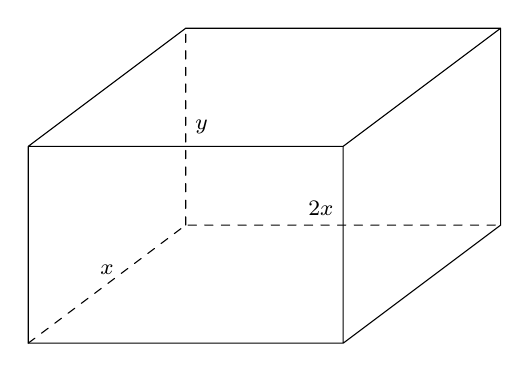
\begin{tikzpicture}[scale=1,font=\footnotesize,line join=round,line cap=round,>=stealth]
				\path 
					(0,0) coordinate  (A)
					(4,0) coordinate  (B)
					 (6,1.5) coordinate (C)
					(2,1.5) coordinate (D) 
					(0,2.5) coordinate  (A')
					(4,2.5)  coordinate (B')
					(6,4) coordinate (C') 
					 (2,4) coordinate (D');
				\draw  (A)--(B)--(C)
					(A')--(B')--(C')--(D')--(A') 
					(A)--(A') 
					(B)--(B') 
					(C)--(C'); 
				\draw[dashed]  (A)--(D)--(C)
					 (D)--(D');
				\foreach \t/\g in  {}{
					\draw (\t)  circle (.5pt) node[shift={(\g:7pt)},font=\scriptsize]{$ \t $};
				} 
				 \path (A)--(D) node[midway,above]{$x$};
				\path  (D')--(D) node[midway,right]{$y$};
				\path (C)--(D)  node[midway,above left]{$2x$};
			\end{tikzpicture}
		\end{center}
		Gọi $x$, $2x$, $y$ với $x$, $y>0$ lần lượt là chiều rộng,  chiều dài, chiều cao của bể cá.\\
		Theo giả thiết ta  có $2\cdot2xy+2\cdot xy+2x^2=5{,}5\Leftrightarrow6xy+2x^2=5{,}5\Leftrightarrow y=\dfrac{5{,}5-2x^2}{6x}$.\\
		Do $y>0$ nên $5{,}5-2x^2>0$, suy ra $0<x<\dfrac{\sqrt{11}}{2}$.\\ 
		Thể tích bể cá  là $V(x)=2x^2y=2x^2\cdot\dfrac{5{,}5-2x^2}{6x}=-\dfrac{2}{3}x^3+\dfrac{11}{6}x$.\\
		Xét hàm  số $V(x)=-\dfrac{2}{3}x^3+\dfrac{11}{6}x$ trên khoảng $\left(0;\dfrac{\sqrt{11}}{2}\right)$.\\
		Ta có $V^{\prime}(x)=-2x^2+\dfrac{11}{6}=0\Leftrightarrow x=\sqrt{\dfrac{11}{12}}$.\\ 
		Bảng  biến thiên:
		\begin{center}
			
\begin{tikzpicture}
				 \tkzTabInit[nocadre=false,lgt=1.2,espcl=3,deltacl=1]
					 {$x$/1.5,$V'$/0.7,$V$/2}
					{$0$,$\sqrt{\frac{11}{12}}$,$\frac{\sqrt{11}}{2}$} 
				 \tkzTabLine{,+,$0$,-,}
				 \tkzTabVar{-/,+/$y_0$,-/}
			\end{tikzpicture}
		\end{center}
		Thể tích lớn nhất của  bể cá là $V\left(\sqrt{\dfrac{11}{12}}\right)=1{,}17$ m$^3$.
	 }
\end{ex}

% nguồn: Phan1_Lop_12_Dai_so_Chuong_1
\begin{ex}%[2D1V3-6]%[ma:aad5645e]
	Một xưởng sản xuất những thùng hình hộp chữ nhật bằng nhôm không nắp và  có các kích thước $x, y, z$ (dm). Biết tỉ số hai cạnh đáy là $x:y=1:3$, thể tích khối hộp bằng $18\,\text{ dm}^3$. Để tốn ít vật liệu nhất thì tổng $x+y+z$ bằng
	 \choice
		{$10$  dm}
		 {$\dfrac{26}{3}$ dm}
		 {$26$ dm}
		{\True $\dfrac{19}{2}$ dm} 
	\loigiai{ 
		Thể tích khối hộp là  $V=xyz=3x^2z=18\Rightarrow z=\dfrac{6}{x^2}$.\hfill $(1)$\\
		Diện tích nhôm cần sử dụng để sản xuất  khối hộp là $S=xy+2(yz+zx)$.\hfill $(2)$\\
		Thay $(1)$ vào $(2)$ ta có $S=3x^2+\dfrac{48}{x}$ suy ra $S'=6x-\dfrac{48}{x^2}$.\\ 
		 Xét phương trình $S'(x)=0\Leftrightarrow 6x-\dfrac{48}{x^2} = 0\Leftrightarrow x=2$.
		\begin{center}
			
\begin{tikzpicture}[font=\footnotesize,>=stealth]
				 \tkzTabInit[nocadre=false,
					 lgt=1.2,
					espcl=3.5, 
					 deltacl=0.6,
					lw=.75pt,color] 
					{$x$ /1,$S'(x)$ /1,$S (x)$ /2.5} 
					 {$0$,$3$,$+\infty$}
				\tkzTabLine{,+,$0$,-,} 
				\tkzTabVar{-/,+/$S  (2)$,-/}
			\end{tikzpicture}
		\end{center}
		Qua  bảng biến thiên ta thấy $S$ đạt giá trị nhỏ nhất khi $x=2$. \\
		 Khi đó, $y=6$, $z=\dfrac{3}{2}$.\\
		 Khi đó $x+y+z=\dfrac{19}{2}$.
	 }
\end{ex}

% nguồn: Phan1_Lop_12_Dai_so_Chuong_1
\begin{ex}%[2D1V3-6]%[ma:d1aee22f]
	 \immini{
	Từ một tấm tôn có hình dạng là nửa hình tròn bán kính $R=3$, người ta muốn cắt ra một hình chữ nhật (hình vẽ bên). Diện tích lớn nhất có thể của tấm  tôn hình chữ nhật là
	 \choice
		 {$\dfrac{9}{2}$}
		{$6\sqrt2$} 
		{$9\sqrt2$} 
		 {\True $9$}
		}{ 
		\begin{tikzpicture}[scale=0.7]
			\draw  (-3,0)--(-2.99,2.65)--(2.99,2.65)--(3,0);
			 \draw[smooth,samples=100,variable=\t,domain=0:180] plot ({(4)*cos (\t)},{(4)*sin (\t)})--cycle;
			\draw (0,0) circle (1pt) node[below]{$O$}; 
			 \draw (-3,0) circle (1pt) node[below]{$Q$};
			 \draw (3,0) circle (1pt) node[below]{$P$};
			\draw (-2.99,2.65) circle (1pt)  node[left]{$M$};
			\draw (2.99,2.65)  circle (1pt) node[right]{$N$};
			\draw[pattern=north  east lines,pattern color=black!50!] (-3,0)--(-2.99,2.65)--(2.99,2.65)--(3,0);
		\end{tikzpicture}
		 }
	 \loigiai{
		Đặt $OQ=x,\ (0<x<3)  \Rightarrow MQ=\sqrt{MO^2-OQ^2}=\sqrt{9-x^2}$.\\
		Ta  có $S_{MNPQ}=PQ\cdot MQ=2x\cdot\sqrt{9-x^2}\le 2\cdot\dfrac{x^2+9-x^2}{2}=9.$\\
		 Dấu \lq\lq=\rq\rq\ xảy ra khi $x=\dfrac{3\sqrt{2}}{2}.$\\
		Vậy diện tích lớn nhất của tấm tôn bằng $9$. 
	 }
\end{ex}

% nguồn: Phan1_Lop_12_Dai_so_Chuong_1
\begin{ex}%[2D1V3-6]%[ma:5dad4f63]
	 \immini{
	Từ một tấm tôn có hình dạng là nửa hình tròn  bán kính $R=3$, người ta muốn cắt ra một hình chữ nhật (hình vẽ bên). Diện tích lớn nhất có thể của tấm tôn hình chữ nhật là
	\choice 
		 {$\dfrac{9}{2}$}
		 {$6\sqrt2$}
		{$9\sqrt2$} 
		{\True  $9$}
		}{ 
		\begin{tikzpicture}[scale=0.7]
			\draw  (-3,0)--(-2.99,2.65)--(2.99,2.65)--(3,0);
			\draw[smooth,samples=100,variable=\t,domain=0:180] plot  ({(4)*cos (\t)},{(4)*sin (\t)})--cycle;
			\draw (0,0) circle (1pt)  node[below]{$O$};
			\draw (-3,0) circle (1pt)  node[below]{$Q$};
			\draw (3,0)  circle (1pt) node[below]{$P$};
			 \draw (-2.99,2.65) circle (1pt) node[left]{$M$};
			\draw (2.99,2.65)  circle (1pt) node[right]{$N$};
			\draw[pattern=north east lines,pattern color=gray!50] (-3,0)--(-2.99,2.65)--(2.99,2.65)--(3,0); 
		\end{tikzpicture}
		 }
	\loigiai{ 
		 Đặt $OQ=x,\ (0<x<3) \Rightarrow MQ=\sqrt{MO^2-OQ^2}=\sqrt{9-x^2}$.\\
		Ta  có $S_{MNPQ}=PQ\cdot MQ=2x\cdot\sqrt{9-x^2}\le 2\cdot\dfrac{x^2+9-x^2}{2}=9.$\\
		Dấu \lq\lq=\rq\rq\ xảy  ra khi $x=\dfrac{3\sqrt{2}}{2}.$\\
		Vậy diện tích lớn nhất của tấm tôn bằng $9$. 
	} 
\end{ex}

% nguồn: Phan1_Lop_12_Dai_so_Chuong_1
\begin{ex}%[2D1V3-6]%[ma:736e3e0c]
	Cho một tấm tôn hình chữ nhật có kích thước $10 \mathrm{~cm} \times 16 \mathrm{~cm}$. Người ta cắt bỏ $4$ góc của tấm tôn $4$ miếng hình vuông bằng nhau rồi gò lại thành một hình hộp chữ nhật không có nắp. Để thể tích của hình hộp  đó lớn nhất thì độ dài cạnh hình vuông của các miếng tôn bị cắt bỏ bằng
	\begin{center}
		\begin{tikzpicture}[line join=round,line cap=round,line width=.6pt,font=\footnotesize,scale=.8]
			\coordinate (E) at (-6,4); 
			 \coordinate (E1) at ($(E)+(0.5,0)$);
			 \coordinate (F) at (-2,4);
			\coordinate (E2) at  ($(F)-(0.5,0)$);
			\coordinate  (F1) at ($(F)-(0,0.5)$);
			\coordinate (G) at  (-2,0);
			\coordinate  (F2) at ($(G)+(0,0.5)$);
			\coordinate (G1) at  (-2.5,0);
			\coordinate (G2) at (-5.5,0); 
			\coordinate (H) at  (-6,0);
			\coordinate (H1) at ($(E)-(0,0.5)$); 
			\coordinate (H2)  at ($(H)+(0,0.5)$);
			\coordinate  (B) at (0,0);
			\coordinate (A) at (1,.8); 
			\coordinate (C) at (4,0); 
			\coordinate (D) at  ($(C)-(B)+(A)$);
			 \coordinate (A1) at ($(A)+(90:2)$);
			\coordinate (B1)  at ($(B)-(A)+(A1)$);
			\coordinate (C1) at ($(C)-(A)+(A1)$); 
			\coordinate (D1)  at ($(D)-(A)+(A1)$);
			\draw (B1)--(B)--(C)--(D)--(D1)--(A1)--(B1)--(C1)--(D1) 
				(C)--(C1) 
				(E)--(F)--(G)--(H)--cycle  (E1)--(G2)
				(E2)--(G1) 
				(H1)--(F1) 
				 (H2)--(F2);
			 \draw[dashed] (A)--(D)
				(A1)--(A)--(B); 
			\draw[pattern =  north east lines,line width = 1.2pt] (E1)--(-5.5,3.5)--(H1)--(E)--cycle;
			 \draw[pattern = north east lines,line width = 1.2pt] (E2)--(-2.5,3.5)--(F1)--(F)--cycle;
			 \draw[pattern = north east lines,line width = 1.2pt] (G1)--(-2.5,0.5)--(F2)--(G)--cycle;
			 \draw[pattern = north east lines,line width = 1.2pt] (G2)--(-5.5,0.5)--(H2)--(H)--cycle;
			\fill (A) circle (1.5pt) 
				(B)  circle (1.5pt)
				(C) circle (1.5pt) 
				(D)  circle (1.5pt)
				(A1) circle (1.5pt) 
				(B1)  circle (1.5pt)
				(C1) circle (1.5pt) 
				 (D1) circle (1.5pt);
		\end{tikzpicture}
	\end{center}
	 \choice
		{$3$  cm}
		 {$4$ cm}
		{$5$  cm}
		{\True $2$  cm}
	\loigiai{Giả sử độ dài cạnh  hình vuông của các miếng tôn bị cắt bỏ bằng $x$, $(0<2 x<10$, $0<x<5)$.\\
		Khi  đó hình hộp chữ nhật có chiều cao bằng $x$, chiều rộng bằng $10-2 x$ và chiều dài bằng $16-2 x$.\\
		Suy ra hình hộp chữ nhật có thể tích $V=x(10-2 x)(16-2 x)=4 x^{3}-52 x^{2}+160  x$.\\
		Xét hàm số $f(x)=4 x^{3}-52 x^{2}+160 x$ trên  $(0; 5)$ có tập xác định là $\mathscr{D}=\mathbb{R}$.\\
		Ta  có
		$f'(x)=12  x^{2}-104 x+160=0 \Leftrightarrow\hoac{&x=2 \\ &x=\dfrac{20}{3}.}$ \\
		Bảng biến thiên hàm số $f(x)$  trên $(0; 5)$ như sau:
		\begin{center}
			
\begin{tikzpicture}
				 \tkzTabInit[espcl=2.5,lgt=1.5]
					 {$x$/0.7,$y'$/0.7,$y$/2.1}
					 {$0$,$2$,$5$}
				 \tkzTabLine{,+,0,-,}
				\tkzTabVar{-/$ $,+/$ $,-/$ $} 
			\end{tikzpicture}
		\end{center}
	Dựa vào bảng biến thiên ta có hàm số đạt giá trị lớn nhất trên $(0; 5)$ tại $x=2$  hay hình hộp chữ nhật có thể tích lớn nhất khi độ dài cạnh hình vuông của miếng tôn bị cắt bỏ bằng $2$ cm.}
\end{ex}

% nguồn: Phan1_Lop_12_Dai_so_Chuong_1
\begin{ex}%[2D1V3-6]%[ma:9c577bce]
	Tam giác vuông có cạnh huyền bằng $5$ cm  có thể có diện tích lớn nhất bằng bao nhiêu cm$^2$?
	\choice 
		{$25$} 
		 {$\dfrac{125}{4}$}
		{\True  $\dfrac{625}{4}$}
		 {$125$}
	\loigiai{Gọi  một cạnh góc vuông là $x~(0<x<5)$ thì cạnh góc vuông còn lại là $\sqrt{25-x^{2}}$.\\
		Như  vậy, diện tích $S=\dfrac{x \sqrt{25-x^{2}}}{2}$. Đặt $f(x)=25 x^{2}-x^{4}$.\\
		Ta có $f^{\prime}(x)=50 x-4 x^{3}$. Khi đó $f^{\prime}(x)=0 \Rightarrow x=\dfrac{5  \sqrt{2}}{2}$.\\
		Vì vậy $\max\limits_{(0; 5)} f(x)=f\left(\dfrac{5  \sqrt{2}}{2}\right)=\dfrac{625}{4}$.\\
	Vậy tam giác vuông có cạnh huyền bằng $5$ cm có thể  có diện tích lớn nhất bằng $\dfrac{625}{4}$ cm$^2$.}
\end{ex}

% nguồn: Phan1_Lop_12_Dai_so_Chuong_1
\begin{ex}%[2D1V3-6]%[ma:44428c28]
	\immini{Người ta muốn xây một chiếc bể nước có hình dạng là một khối hộp chữ nhật không nắp có thể tích bằng $\dfrac{500}{3} \mathrm{~m}^{3}$. Biết đáy bể là một hình chữ nhật có chiều dài gấp đôi chiều rộng và giá thuê thợ xây là $700\,000$ đồng $/ \mathrm{m}^{2}$. Người ta tính được kích thước của bể để chi phí thuê nhân công ít nhất. Khi đó chi phí thuê nhân công là}{\begin{tikzpicture}[line join=round,line cap=round,>=stealth,font=\footnotesize,scale=0.5]
		\def\a{5} 
		\def\b{2} 
		\def\h{3.5} 
		\path (0:0) coordinate (A) 
			++(0:\a) coordinate (D) 
			++(-130:\b) coordinate (C) 
			($(A)+(C)-(D)$) coordinate  (B)
			($(A)+(90:\h)$) coordinate (A') 
			($(B)+(90:\h)$) coordinate (B') 
			($(C)+(90:\h)$) coordinate (C') 
			($(D)+(90:\h)$)  coordinate (D');
		 \draw[dashed] (B)--(A)--(D)
			 (A)--(A');
		\draw  (C)--(C')
			 (D)--(D')
			 (B)--(B')
			(C)--(C') 
			 (B)--(C)--(D)
			 (A')--(B')--(C')--(D')--cycle;
	\end{tikzpicture}
	 }
	\choice 
		{$120$ triệu  đồng}
		{\True $105$ triệu  đồng}
		 {$115$ triệu đồng}
		{$110$  triệu đồng}
	\loigiai{Gọi $x, y$ lần lượt là chiều rộng và  chiều cao của bể cá (điều kiện $x, y>0$).\\
		Với giả thiết  của bài toán, thể tích bể cá là $V=2 x^{2} y=\dfrac{500}{3} \Rightarrow y=\dfrac{250}{3 x^{2}}$.\\
		Để chi phí thuê nhân công ít nhất thì tổng diện tích các mặt của  bể cá phải nhỏ nhất.\\
		Tổng diện tích các mặt của bể cá $S=2 x  y+2\cdot2 x y+2 x^{2}=6 x y+2 x^{2}=\dfrac{500}{x}+2 x^{2}$.\\
		Xét hàm số $S(x)=\dfrac{500}{x}+2 x^{2}$ trên khoảng $(0;+\infty)$. \\ 
		Ta  có $S'(x)=-\dfrac{500}{x^{2}}+4 x=0 \Leftrightarrow x=5$. Bảng biến thiên
		\begin{center}
			
\begin{tikzpicture}
				 \tkzTabInit[lgt=2,espcl=3]
					{$x$/1,$S'(x)$/1,$S (x)$/2} 
					 {$0$,$5$,$+\infty$}
				\tkzTabLine{,-,z,+,} 
				 \tkzTabVar{+/$+\infty$,-/$150$,+/$+\infty$}
			\end{tikzpicture}
		\end{center}
		Do đó $\min  S=150$ tại $x=5$.\\
	Khi đó chi phí thuê nhân  công là $T=150\cdot700\,000=105$ triệu đồng.}
\end{ex}

% nguồn: Phan1_Lop_12_Dai_so_Chuong_1
\begin{ex}%[2D1V3-6]%[ma:12e3c532]
	\immini 
	{Từ hình vuông có cạnh bằng $6$ người ta cắt bỏ các tam giác vuông cân tạo thành hình tô đậm như hình vẽ. Sau đó người ta gập thành  hình hộp chữ nhật không nắp. Tính thể tích lớn nhất của khối hộp.
	\choice 
		{\True  $8\sqrt {2}$}
		 {$10\sqrt{2}$}
		{$9\sqrt  {2}$}
		 {$11\sqrt{2}$}
		 }
		{\begin{tikzpicture}[join = round,cap = round,font = \small,scale = 0.6]
		 \def\canh{6}
		\path 
			(0:0)  coordinate (A)
			 ++(0:\canh) coordinate (B)
			 ++(-90:\canh) coordinate (C)
			 ($(A)+(C)-(B)$) coordinate (D)
			($(A)!1/3!(B)$) coordinate  (A1)
			($(A)!2/3!(B)$) coordinate  (A2)
			($(B)!1/3!(C)$) coordinate (B1) 
			($(B)!2/3!(C)$)  coordinate (B2)
			($(C)!1/3!(D)$) coordinate (C1) 
			($(C)!2/3!(D)$) coordinate  (C2)
			 ($(D)!1/3!(A)$) coordinate (D1)
			($(D)!2/3!(A)$)  coordinate (D2)
			(intersection of  A1--B2 and A2--D1) coordinate (I)
			(intersection of A1--B2 and B1--C2)  coordinate (J)
			(intersection of C1--D2 and B1--C2) coordinate (K) 
			(intersection of A2--D1 and C1--D2) coordinate (L); 
		 \draw (A)--(B)--(C)--(D)--cycle (A1)--(B2)--(C1)--(D2)--cycle
			(A2)--(B1)--(C2)--(D1)--cycle; 
		\fill[gray!20]  (A1)--(I)--(A2)--(B1)--(J)--(B2)--(C1)--(K)--(C2)--(D1)--(L)--(D2);
	\end{tikzpicture}
		} 
	\loigiai{ 
	\immini 
		{Đặt kích thước các cạnh  như hình vẽ.\\
		Ta có $\dfrac{x}{\sqrt{2}} + y\sqrt{2} + \dfrac{x}{\sqrt{2}} = 6 \Leftrightarrow x + y = 3\sqrt{2} \Leftrightarrow y = 3\sqrt {2} - x$ với $0 <  x < 3\sqrt {2}$.\\
		Thể tích của  khối hộp tạo thành là
		$$V =  x^2y = x^2\left(3\sqrt{2} - x\right).$$
		Khi đó $V' = 3x\left(2\sqrt{2} - x  \right)$.\\
		Suy ra $V'  = 0 \Rightarrow x = 2\sqrt{2}$.
		 }
		{\begin{tikzpicture}[join = round,cap = round,font = \small,scale = 0.6]
		\def\canh{6} 
		\path 
			(0:0) coordinate (A) 
			++(0:\canh) coordinate  (B)
			++(-90:\canh) coordinate  (C)
			($(A)+(C)-(B)$) coordinate (D) 
			($(A)!1/3!(B)$) coordinate (A1) 
			($(A)!2/3!(B)$) coordinate  (A2)
			($(B)!1/3!(C)$) coordinate  (B1)
			 ($(B)!2/3!(C)$) coordinate (B2)
			($(C)!1/3!(D)$) coordinate (C1) 
			($(C)!2/3!(D)$)  coordinate (C2)
			($(D)!1/3!(A)$) coordinate (D1) 
			 ($(D)!2/3!(A)$) coordinate (D2)
			(intersection of A1--B2 and A2--D1) coordinate (I) 
			(intersection of A1--B2  and B1--C2) coordinate (J)
			(intersection of C1--D2 and B1--C2) coordinate (K) 
			(intersection of A2--D1 and  C1--D2) coordinate (L);
		 \draw (A)--(B)--(C)--(D)--cycle (A1)--(B2)--(C1)--(D2)--cycle
			 (A2)--(B1)--(C2)--(D1)--cycle;
		 \fill[red!20,opacity=0.5] (A1)--(I)--(A2)--(B1)--(J)--(B2)--(C1)--(K)--(C2)--(D1)--(L)--(D2);
		\path (0.8,-0.6)  node{$x$};
		\path  (3.0,-0.5) node{$y$};
	\end{tikzpicture}
		}\noindent 
		Bảng biến thiên 
		\begin{center}
			
\begin{tikzpicture}
				 \tkzTabInit[lgt=1.2,espcl=4]
					{$x$/1,$V'(x)$/1,$V  (x)$/2}
					 {$0$,$2\sqrt{2}$,$3\sqrt{2}$}
				 \tkzTabLine{,+,$0$,-,}
				\tkzTabVar{-/,+/$8\sqrt{2}$,-/} 
			\end{tikzpicture}
		\end{center}
		Vậy  $V_{\max} = 8\sqrt{2}$ khi $x = 2\sqrt{2}$, $y=\sqrt{2}$.
	} 
\end{ex}

% nguồn: Phan1_Lop_12_Dai_so_Chuong_1
\begin{ex}%[2D1V3-6]%[ma:e5063647]
	\immini{ 
	Một người thợ gò làm một cái hòm dạng hình hộp chữ nhật \textit{có nắp} bằng tôn. Biết rằng độ dài đường chéo hình hộp bằng $3\sqrt{2}$ dm và chỉ được sử dụng vừa đủ $18$ dm$^2$ tôn. Với yêu cầu như trên người thợ có  thể làm được cái hòm có thể tích lớn nhất bằng
	 \choice
		{$8$  dm$^3$}
		{$2 \sqrt{2}$  dm$^3$}
		{$6$  dm$^3$}
		{\True $4$  dm$^3$}}{
		\begin{tikzpicture}[line join=round,line cap=round,>=stealth]
			 \def\a{4}
			 \def\b{2}
			 \def\h{2}
			\path  (0:0) coordinate (A)
				++(0:\a) coordinate (D) 
				++(-130:\b)  coordinate (C)
				($(A)+(C)-(D)$) coordinate  (B)
				($(A)+(90:\h)$) coordinate (A') 
				 ($(B)+(90:\h)$) coordinate (B')
				($(C)+(90:\h)$) coordinate  (C')
				($(D)+(90:\h)$) coordinate  (D');
			\draw[dashed] (B)--(A)--(D) 
				 (A)--(A');
			 \draw (C)--(C')
				 (D)--(D')
				(B)--(B') 
				 (C)--(C')
				 (B)--(C)--(D)
				 (A')--(B')--(C')--(D')--cycle;
		\end{tikzpicture}
		 }
	 \loigiai{
		Gọi $a$, $b$, $c$ ($a>0$, $b>0$, $c>0$) là $3$ kích thước của hình hộp chữ nhật. Không mất tính tổng quát,  giả sử $0<c \leq b \leq a$.\\
		Theo  giả thiết $\sqrt{a^2+b^2+c^2}=3 \sqrt{2} \Rightarrow a^2+b^2+c^2=18. \quad (1)$\\
		Diện tích toàn phần của  khối hộp là $2a b+2b c+2c a=18. \quad(2)$\\
		Từ $(1)$, $(2)$ ta có $(a+b+c)^2=a^2+b^2+c^2+2a b+2b c+2c  a=36 \Rightarrow a+b+c=6. \quad (3)$\\
		Từ $(3)$,  $(2)$ ta có $a b+c(6-c)=9 \Rightarrow a b=9+c^2-6c$.\\
		Thể tích của cái hòm $V=a b c=\left(c^2-6c+9\right) c=c^3-6c^2+9c,  \,(0<c<\sqrt{6})$.\\
		Đặt $h(c)=c^3-6c^2+9c \Rightarrow h'(c)=3c^2-12c+9 \Rightarrow h'(c)=0 \Leftrightarrow \hoac{&c=1 \quad \text{ (nhận)}\\& c=3 \quad  \text{ (loại)}.}$\\
		 Bảng biến thiên
		\begin{center}
			
\begin{tikzpicture}[scale=1,font=\footnotesize,line join=round,line cap=round,>=stealth]
				 \tkzTabInit[nocadre=false,lgt=1.5,espcl=3,deltacl=1.5]
					{$c$/.7,$h'(c)$/.7,$h (c)$/2.5} 
					{$0$,$1$,$\sqrt{6}$} 
				\tkzTabLine{,+,$0$,-,} 
				 \tkzTabVar{-/$0$,+/$4$,-/$-36+15\sqrt{6}$}
			\end{tikzpicture}
		\end{center}
		 Vậy thể tích lớn nhất bằng $4$ dm$^3$.
	} 
\end{ex}

% nguồn: Phan1_Lop_12_Dai_so_Chuong_1
\begin{ex}%[2D1V3-6]%[ma:89e14de6]
	Độ giảm huyết áp của một bệnh nhân được cho bởi công thức\break $G(x)=0{,}025 x^{2}(30-x)$, trong đó $x$ là liều lượng thuốc được tiêm cho bệnh nhân ($x$ được  tính bằng miligam). Liều lượng thuốc cần tiêm cho bệnh nhân là bao nhiêu để huyết áp được giảm nhanh nhất?
	 \choice
		 {$24$ mg}
		{\True $20$  mg}
		 {$15$ mg}
		{$10$  mg}
	\loigiai{ 
		Bài toán  trở thành tìm $x \in[0; 30]$ để hàm số $G(x)=0{,}025 x^{2}(30-x)$ đạt giá trị lớn nhất.\\
		Ta có $G(x)=0{,}025 x^{2}(30-x) \Rightarrow  G'(x)=0{,}025\left(60 x-3 x^{2}\right)=0 \Leftrightarrow\hoac{&x=0 \\ &x=20.}$\\
		Ta có  $G(0)=G(30)=0$; $G(20)=100$. Suy ra $\max\limits_{[0; 30]} G(x)=G(20)=100$.\\
	Vậy liều lượng thuốc cần tiêm cho  bệnh nhân để huyết áp giảm nhanh nhất là $20$ mg.}
\end{ex}

% nguồn: Phan1_Lop_12_Dai_so_Chuong_1
\begin{ex}%[2D1V3-6]%[ma:8a5626fb]
	Trong $3$ giây đầu tiên, một chất điểm chuyển động theo phương trình\break $s(t)=-t^3+6t^2+t+5$, trong đó $t$ tính bằng giây và $s$ tính bằng mét. Chất điểm có vận tốc  tức thời lớn nhất bằng bao nhiêu trong $3$ giây đầu tiên đó?
	\choice 
		 {$13$ m/s}
		 {$10$ m/s}
		 {$9$ m/s}
		 {\True $12$ m/s}
	 \loigiai{Ta có $v(t)=s'(t)=-3t^2+12t+1$. Xét hàm số $v(t)=-3t^2+12t+1$ trên đoạn $[0;3]$.\\
		$v'(t)=-6t+12=0\Leftrightarrow  t=2$.\\
		Tính các giá trị $v(0)=1$;  $v(2)=13$; $v(3)=10$.\\
		So sánh các giá trị, ta  suy ra $\max\limits_{[0;3]}v(t)=13$.
	 }
\end{ex}

% nguồn: Phan1_Lop_12_Dai_so_Chuong_1
\begin{ex}%[2D1V3-6]%[ma:d13d7904]
	\immini{Từ một tấm tôn có hình dạng là nửa hình tròn bán kính $R=3$, người ta muốn cắt ra một hình chữ nhật (hình vẽ bên). Diện tích lớn nhất có thể của tấm tôn hình chữ nhật là}{\begin{tikzpicture}[scale=0.8,font=\footnotesize,line join=round,line cap=round,>=stealth]
		\path 
			(-2.25,0)  coordinate (Q)
			 (-2.25,1.99) coordinate (M)
			(2.23,2.01) coordinate  (N)
			 (2.23,0) coordinate (P)
			(0,0) coordinate (O) 
			 (-3,0) coordinate (E)
			(3,0) coordinate (F); 
		\draw (3,0) arc (0:180:3); 
		\draw  (M)--(N)--(P)--(Q)--(M)
			(E)--(F); 
		 \fill[pattern=north west lines](M)--(N)--(P)--(Q)--cycle;
		\foreach \i/\g in {M/120,N/20,P/-90,Q/-90,O/-90} 
		 \fill (\i) circle (1pt)+(\g:4mm) node[scale=1]{$\i$};
	\end{tikzpicture}
	 }
	\choice 
		{$\dfrac{9}{2}$} 
		 {$6\sqrt{2}$}
		 {\True $9$}
		{$9\sqrt{2}$} 
	\loigiai{Đặt  $OQ=x$, ($0<x<3$) suy ra $MQ=\sqrt{MO^2-OQ^2}=\sqrt{9-x^2}$.\\
		Ta có $S_{NMPQ}=PQ\cdot MQ=2x\cdot\sqrt{9-x^2}\leq 2\cdot\dfrac{x^2+9-x^2}{2}=9$.\\ 
		Dấu \lq\lq=\rq\rq \  xảy ra khi $x^2=9-x^2 \Leftrightarrow x=\dfrac{3\sqrt{2}}{2}$.
	} 
\end{ex}

% nguồn: Phan1_Lop_12_Dai_so_Chuong_1
\begin{ex}%[2D1V3-6]%[ma:f5eefc25]
	Một công ty bất động sản có $40$ căn hộ cho thuê. Biết rằng nếu cho thuê mỗi căn hộ với giá $3\,000\,000$ đồng một tháng thì mọi căn hộ đều có người thuê và cứ tăng thêm giá mỗi căn hộ $100\,000$ đồng một tháng (theo quy định trong hợp  đồng) thì sẽ có một căn hộ bị bỏ trống. Hỏi muốn có thu nhập cao nhất thì công ty đó phải cho thuê mỗi căn hộ với giá bao nhiêu một tháng?
	\choice 
		{\True $3\,500\,000$  đồng}
		 {$4\,000\,000$ đồng}
		{$3\,700.000$  đồng}
		{$3\,900\,000$  đồng}
	 \loigiai{
		Gọi  $x$ là số căn hộ bị bỏ trống $\left(0 \le x \le 40\right)$.\\
		Vậy giá cho thuê một căn phòng là  $3+0{,}1x$ (triệu đồng).\\
		Số căn hộ cho thuê là  $40-x$. \\
		Số  tiền thu được là
		$$T=(40-x) \cdot (3+0{,}1x)=-0{,}1x^2+x+120 \Rightarrow T'=-0{,}2x+1 \Rightarrow T'=0 \Rightarrow x=5.$$ 
		Ta có  bảng biến thiên
		\begin{center}
			
\begin{tikzpicture}
				\tkzTabInit[espcl=2.5,lgt=1.5] 
					 {$x$/0.7,$T'$/0.7,$T$/2.1}
					 {$0$,$5$,$40$}
				 \tkzTabLine{,+,0,-,}
				\tkzTabVar{-/$ $,+/$122{,}5$,-/$ $} 
			\end{tikzpicture}
		\end{center}
		Vậy $T$ đạt giá trị  lớn nhất khi $x=5$, khi đó giá thuê một căn phòng là $3\,500\,000$ đồng.
	 }
\end{ex}

% nguồn: Phan1_Lop_12_Dai_so_Chuong_1
\begin{ex}%[2D1V3-6]%[ma:66445fe5]
	Một chất điểm chuyển động với quãng đường $s(t)$ cho bởi công thức \break $s(t)=6 t^{2}-t^{3}$, $t$ (giây) là thời gian. Hỏi từ $0$ đến $4$ giây, vận tốc tức thời của chất điểm  đạt giá trị lớn nhất tại thời điểm $t$ (giây) bằng bao nhiêu?
	 \choice
		 {$t=3$}
		 {$t=4$}
		{\True  $t=2$}
		{$t=6$} 
	\loigiai{Ta có $v(t)=s'(t)=12 t-3 t^{2}$;  $v'(t)=12-6 t=0 \Leftrightarrow t=2$.\\
		Ta có $v(0)=0$;  $v(2)=12$; $v(4)=0$.\\
	Suy ra $v(t)$ đạt giá trị lớn nhất  tại $t=2$ giây.}
\end{ex}

% nguồn: Phan1_Lop_12_Dai_so_Chuong_1
\begin{ex}%[2D1V3-6]%[ma:a27fcb6b]
	Một thanh sắt chiều dài $AB=100$ m được cắt thành hai phần $AC$ và $CB$ với $AC=x$ (m). Đoạn $AC$ được uốn thành một hình vuông có chu vi bằng $AC$ và đoạn $CB$ uốn thành tam giác đều  có chu vi bằng $CB$. Khi tổng diện tích của hình vuông và tam giác nhỏ nhất, mệnh đề nào dưới đây đúng?
	\begin{center}
		\begin{tikzpicture}[scale=0.7,font=\footnotesize,line join=round,line cap=round,>=stealth]
			\fill (-6,0) circle (1pt) node[left]{$A$}--(1,0) circle  (1pt) node[above]{$C$}--(6,0) circle (1pt) node[right]{$B$};
			\draw  (-6,0)--(6,0);
			\draw[->] (0,-0.3)--(-2,-1.8); 
			\draw[->]  (0,-0.3)--(2,-1.8);
			\draw (-3,-2)--(-1,-2)--(-1,-4)--(-3,-4)--cycle; 
			\draw  (2,-2)--(0.7,-4)--(3.3,-4)--cycle;
		\end{tikzpicture}
	\end{center}
	 \choice
		{$x\in (52;58)$} 
		{$x\in  (48;52)$}
		{\True  $x\in (40;48)$}
		{$x\in (30;40)$} 
	 \loigiai{
		Theo đề các cạnh của hình vuông có độ dài là $\dfrac{x}{4}$, các cạnh của tam  giác đều có độ dài là $\dfrac{100-x}{3}$.\\
		Ta có $S=\left(\dfrac{x}{4} \right)^2+\left(\dfrac{100-x}{3}\right)^2\cdot\dfrac{\sqrt{3}}{4}= \dfrac{\left( 9+4\sqrt{3}\right)}{144} x^2-\dfrac{800\sqrt{3}}{144}x+\dfrac{40\,000\sqrt{3}}{144}.$\\ 
		 Đây là hàm bậc hai có hệ số $a>0$ nên hàm đạt giá trị nhỏ nhất khi $$x=-\dfrac{b}{2a}=\dfrac{800\sqrt{3}}{144}\cdot \dfrac{144}{2\cdot(9+4\sqrt{3})}\approx 43{,}5 \text{ m}.$$
	} 
\end{ex}

% nguồn: Phan1_Lop_12_Dai_so_Chuong_1
\begin{ex}%[2D1V3-6]%[ma:6313b696]
	\immini{ 
	Máng trượt của một cầu trượt cho trẻ em (\textit{Hình a}) được uốn từ một tấm kim loại có bề rộng $80$ cm, mặt cắt được mô tả ở \textit{Hình b}. Nhà thiết kế khuyến cáo, diện tích mặt cắt càng lớn thì càng đảm bảo an  toàn cho trẻ em.
	}{ 
	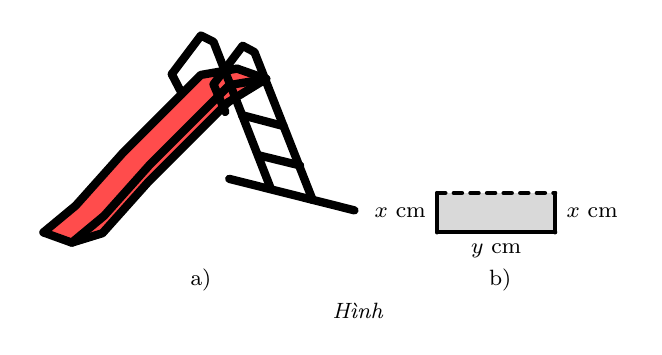
\begin{tikzpicture}[scale=1,font=\footnotesize,line join=round,line cap=round,>=stealth,line width=1.5pt]
		\clip  (-0.2,-1.2) rectangle (7.5,2.6);
		 \fill[red,fill opacity=0.7] (0,0)--(0.41,0.34)--(1,1)--(1.76,1.76)--(2,2)--(2.46,2.08)--(2.83,1.95)--(2.34,1.65)--(1.34,0.65)--(0.75,-0.01)--(0.36,-0.13)-- cycle;
		\begin{scope}[line width=3pt]
			\draw  (0,0)--(0.41,0.34)--(1,1)--(2,2)--(2.46,2.08);
			\draw  (0,0)--(0.36,-0.13)--(0.77,0.21)--(0.77,0.21)--(1.36,0.87)--(2.36,1.87)--(2.83,1.95);
			\draw  (0.36,-0.13)--(0.75,-0.01)--(1.34,0.65)--(2.34,1.65);
			\draw  (2.36,0.68)-- (3.95,0.28);
			 \draw (3.42,0.41)--(2.68,2.29)--(2.53,2.37)--(2.16,1.88)--(2.31,1.53);
			\draw  (1.63,2.01)--(2,2.5)-- (2.16,2.42)--(2.89,0.55);
			 \draw (1.63,2.01)--(1.76,1.76)
				(2.73,0.98)--(3.26,0.85) 
				(2.52,1.49)--(3.05,1.35); 
			 \draw (2.34,1.65)--(2.83,1.95)--(2.46,2.08);
		\end{scope}
		\draw (2,-0.6)  node{a)};
		\fill[line  width=1.5pt,fill=gray,fill opacity=0.3] (5,0.5)--(5,0)--(6.5,0)--(6.5,0.5)--cycle;
		\draw  (5,0.5)--(5,0) node [left,sloped,pos=0.5,rotate=90] {$x$ cm};
		\draw (5,0)--(6.5,0) node [below,sloped,pos=0.5] {$y$ cm}; 
		\draw (6.5,0)--(6.5,0.5)  node [right,sloped,pos=0.5,rotate=-90] {$x$ cm};
		 \draw[dashed] (5,0.5)--(6.5,0.5);
		\draw  (5.8,-0.6) node{b)};
		\draw (4,-1)  node{\textit{Hình}};
	\end{tikzpicture}
	} 
	 \noindent
	Với $x$ đạt giá  trị bằng bao nhiêu thì cầu trượt đảm bảo an toàn nhất cho trẻ em?
	\choice 
		{$x = 16$ cm} 
		{$x=18$  cm}
		{$x=22$ cm} 
		{\True  $x=20$ cm}
	\loigiai{ 
		Do tấm kim loại có bề rộng $80 \mathrm{~cm}$ nên ta có: $2x+y=80 \Leftrightarrow y=80-2x$.\\ 
		Để có thể thiết kế được máng  trượt thì $y>0 \Leftrightarrow 80-2 x>0 \Leftrightarrow x<40$. Suy ra $0<x<40$.\\
		Diện tích  của mặt cắt máng trượt là $S=x y=x(80-2x)=-2x^2+80x$.\\
		Ta có 
		 \allowdisplaybreaks
		\begin{eqnarray*}
			 S(x)&=&-2x^2+80x \text{ với } x\in(0; 40);\\
			 S'(x)&=&-4 x+80 \\
			S'(x)&=&0 \Leftrightarrow-4 x+80=0  \Leftrightarrow x=20.
		\end{eqnarray*}
		Bảng biến thiên  của hàm số $S(x)$ như sau
		\begin{center}
			
\begin{tikzpicture}[font=\footnotesize,>=stealth]
				 \tkzTabInit[nocadre=false,lgt=1.2,espcl=2.5,deltacl=0.6]
					{$x$ /0.7,$S'(x)$ /0.8,$S (x)$  /2}
					{$0$,$20$,$40$} 
				\tkzTabLine{,+,,-,} 
				\tkzTabVar{-/$0$,+/$800$,-/$0$} 
			\end{tikzpicture}
		\end{center}
		Do đó, hàm  số $S(x)$ đạt cực đại tại $x=20$ và $S_{\text{ CĐ}}=800$.\\
		 Vậy để cầu trượt đảm bảo an toàn nhất cho trẻ em thì $x=20$ (cm).
	 }
\end{ex}

% nguồn: Phan1_Lop_12_Dai_so_Chuong_1
\begin{ex}%[2D1C3-6]%[ma:d7bc38d4]
	Tìm diện tích lớn nhất của hình chữ nhật nội tiếp trong nửa đường tròn bán kính $R$, nếu một cạnh của hình chữ  nhật nằm dọc theo đường kính của hình tròn mà hình chữ nhật đó nội tiếp?
	\choice 
		 {$2R^2$}
		 {$5R^2$}
		{\True  $R^2$}
		 {$3R^2$}
	 \loigiai{
		Gọi $x$ là độ dài cạnh của hình chữ nhật không nằm dọc theo  đường kính của hình tròn $( 0<x<R)$\\
		Độ dài cạnh còn lại của hình chữ nhật  là $2\sqrt{R^2 - x^2}$.\\
		Ta có diện tích của hình chữ nhật là $S(x) = 2x\sqrt{R^2 -  x^2}$.\\
		Xét hàm số  $S(x) = 2x\sqrt{R^2 - x^2}$ với $0 < x < R$.\\
		Ta có $S'(x) = 2\sqrt{R^2 - x^2} -  \dfrac{2x^2}{\sqrt{R^2 - x^2}} = \dfrac{2R^2 - 4x^2}{\sqrt{R^2 - x^2}}$.\\
		Khi đó $S'(x) = 0 \Leftrightarrow 2R^2 - 4x^2 = 0 \Leftrightarrow \hoac{&x = \dfrac{R\sqrt{2}}{2} \\&  x = \dfrac{-R\sqrt{2}}{2}.}$\\
		Vì $x  = \dfrac{-R\sqrt{2}}{2} \notin (0;R)$ và $x = \dfrac{R\sqrt{2}}{2} \in (0;R)$ nên ta có bảng biến thiên sau
		\begin{center}
			
\begin{tikzpicture}
				\tkzTabInit[lgt=1.2,espcl=4] 
					 {$x$/1,$S'(x)$/1,$S (x)$/2}
					{$0$,$\dfrac{R\sqrt{2}}{2}$,$R$} 
				\tkzTabLine{,+,$0$,-,} 
				 \tkzTabVar{-/$-\infty$,+/$R^2$,-/$-\infty$}
			\end{tikzpicture}
		\end{center}
		Vậy diện tích lớn nhất của  hình chữ nhật là $R^2$.
	 }
\end{ex}

% nguồn: Phan1_Lop_12_Dai_so_Chuong_1
\begin{ex}%[2D1C3-6]%[ma:72b0c08c]
	 \immini
	{Một khúc gỗ tròn hình trụ cần xẻ thành một chiếc xà có tiết diện ngang là hình vuông và $4$ miếng phụ như hình vẽ. Hãy xác định kích thước của các miếng phụ để diện tích sử dụng theo tiết diện ngang là lớn nhất.  Biết đường kính khúc gỗ là $d$.
	 }
	{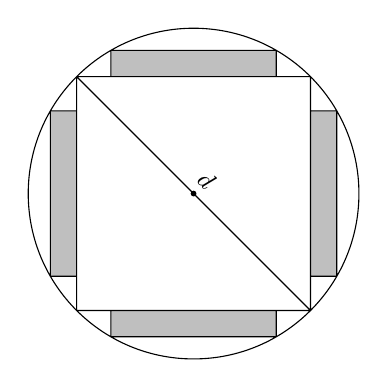
\begin{tikzpicture}[line join = round,line cap = round,>=stealth,font = \small,scale = 0.7]
		 \path
			(0,0) coordinate (O) 
			 +(45:3) coordinate (N)
			+(135:3) coordinate (M) 
			 +(-45:3) coordinate (P)
			 +(-135:3) coordinate (Q)
			+(150:3) coordinate  (A)
			+(30:3) coordinate (B) 
			+(-30:3) coordinate (C) 
			 +(-150:3) coordinate (D)
			+(60:3)  coordinate (F)
			 +(120:3) coordinate (E)
			+(-60:3) coordinate  (G)
			+(-120:3) coordinate (H) 
			(intersection of A--B and M--Q) coordinate  (1)
			 (intersection of A--B and N--P) coordinate (2)
			(intersection of  C--D and M--Q) coordinate (4)
			(intersection of  C--D and N--P) coordinate (3)
			 (intersection of E--H and M--N) coordinate (5)
			(intersection  of F--G and M--N) coordinate (6)
			(intersection of F--G and P--Q) coordinate (7) 
			(intersection of E--H and  Q--P) coordinate (8);
		\fill[gray!50] 
			(E)--(F)--(6)--(5)--cycle 
			(2)--(B)--(C)--(3)--cycle 
			(7)--(G)--(H)--(8)--cycle 
			(1)--(A)--(D)--(4)--cycle; 
		 \draw (O) circle (3)
			(M)--(N)--(P)--(Q)--cycle 
			 (D)--(A)--(1)
			 (C)--(B)--(2)
			 (C)--(3)
			(D)--(4) 
			 (5)--(E)--(F)--(6)
			(7)--(G)--(H)--(8) 
			 (1)--(A)--(D)--(4)
			 (P)--(M) node[midway,sloped,above]{$d$};
		\foreach \x/\g in {O/90}\fill (\x) circle (1.5pt)+(\g:3mm)  node{};
	\end{tikzpicture}
	 }
	 \choice
		{\True  Rộng $\dfrac{\sqrt{34} - 3\sqrt{2}}{16}d$, dài $\dfrac{\sqrt{7 - \sqrt {17}}}{4}d$}
		{Rộng $\dfrac{\sqrt{34}-3\sqrt {2}}{15}d$,  dài $\dfrac{\sqrt{7-\sqrt {17}}}{4}d$}
		{Rộng $\dfrac{\sqrt {34}-3\sqrt {2}}{14}d$, dài $\dfrac{\sqrt{7-\sqrt  {17}}}{4}d$}
		{Rộng $\dfrac{\sqrt {34}-3\sqrt {2}}{13}d$, dài  $\dfrac{\sqrt{7-\sqrt {17}}}{4}d$}
	\loigiai{ 
	\immini 
		{Gọi chiều dài và chiều rộng của miếng phụ lần lượt là $x$, $y$ ($x>0$, $y>0$).\\ 
		Đường kính của khúc gỗ  là $d$, khi đó tiết diện ngang của thanh xà có độ dài cạnh là $\dfrac{d}{\sqrt{2}}$ và \break $0 < x < \dfrac{d\left(2 - \sqrt{2}\right)}{4}$, $0 < y < \dfrac{d}{\sqrt{2}}$.\\
		Theo đề bài ta có $CD = 2x + \dfrac{d}{\sqrt{2}}$;  $AD = y$.\\
		Trong  $\triangle ACD$ ta có
		$$\left(2x + \dfrac{d}{\sqrt{2}} \right)^2 + y^2 = d^2 \Leftrightarrow y = \dfrac{1}{\sqrt{2}}\sqrt{d^2 -  8x^2 - 4\sqrt{2}x}.$$
		} 
		{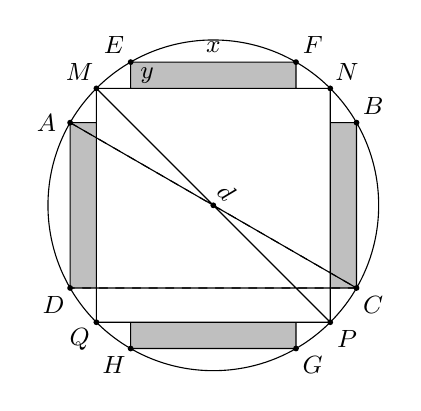
\begin{tikzpicture}[line join = round,line cap = round,>=stealth,font = \small,scale = 0.7]
		 \path
			(0,0) coordinate  (O)
			+(45:3)  coordinate (N)
			+(135:3) coordinate  (M)
			+(-45:3) coordinate (P) 
			+(-135:3) coordinate (Q) 
			 +(150:3) coordinate (A)
			+(30:3) coordinate  (B)
			+(-30:3)  coordinate (C)
			 +(-150:3) coordinate (D)
			+(60:3)  coordinate (F)
			+(120:3) coordinate  (E)
			 +(-60:3) coordinate (G)
			+(-120:3) coordinate  (H)
			(intersection of  A--B and M--Q) coordinate (1)
			(intersection of A--B and  N--P) coordinate (2)
			(intersection of  C--D and M--Q) coordinate (4)
			(intersection of C--D and  N--P) coordinate (3)
			(intersection  of E--H and M--N) coordinate (5)
			(intersection of F--G and M--N)  coordinate (6)
			(intersection  of F--G and P--Q) coordinate (7)
			(intersection of  E--H and Q--P) coordinate (8);
		 \fill[gray!50]
			 (E)--(F)--(6)--(5)--cycle
			(2)--(B)--(C)--(3)--cycle 
			 (7)--(G)--(H)--(8)--cycle
			(1)--(A)--(D)--(4)--cycle; 
		\draw (O) circle  (3)
			(M)--(N)--(P)--(Q)--cycle 
			 (D)--(A)--(1)
			(C)--(B)--(2) 
			(C)--(3) 
			 (D)--(4)
			 (5)--(E)--(F)--(6)
			(7)--(G)--(H)--(8) 
			(1)--(A)--(D)--(4) 
			 (A)--(C)--(D)
			(P)--(M) node[midway,sloped,above]{$d$}; 
		\draw[dashed]  (A)--(C)
			 (C)--(D);
		\foreach \x/\g  in {O/90}
		\fill (\x) circle (1.5pt)+(\g:3mm) node{}; 
		\path  (E)--(F) node[midway,sloped,above]{$x$};
		 \path (E)--(5) node[midway,right]{$y$};
		\foreach \p/\r in {A/180,B/45,C/-45,D/225,M/135,N/45,P/-45,Q/-135,E/135,F/45,G/-45,H/-135} 
		\fill  (\p) circle (1.5pt) node[shift={(\r:3mm)}]{$\p$};
	\end{tikzpicture}
		}\noindent 
		Do đó, miếng phụ có  diện tích là $S(x) = \dfrac{1}{\sqrt{2}}\sqrt{d^2 - 8x^2 - 4\sqrt{2}dx}$ với $0 < x < \dfrac{d\left(2 - \sqrt{2} \right)}{4}$.\\
		Bài toán trở thành tìm $x$ để $S(x)$ đạt giá  trị lớn nhất.\\
		Ta có  $S'(x) = \dfrac{1}{\sqrt{2}}\sqrt{d^2 - 8x^2 - 4\sqrt{2}dx} + \dfrac{x\left(-8x - 2\sqrt{2}d \right)}{\sqrt{2}\sqrt {d^2 - 8x^2 - 4\sqrt {2}\mathrm{\,d}x}}$$=\dfrac{-16{x^2}-6\sqrt{2}dx + d^2}{\sqrt{2}\sqrt{d^2 - 8x^2 - 4\sqrt{2}dx}}$.\\
		Khi đó $S'(x) = 0 \Leftrightarrow -16x^2  - 6\sqrt{2}dx + d^2 = 0 \Leftrightarrow -16\left(\dfrac{x}{d}\right)^2 - 6\sqrt{2}\left(\dfrac{x}{d}\right) + 1 = 0 \Leftrightarrow x = \dfrac{\sqrt{34} - 3\sqrt{2}}{16}d$.\\
		Vậy miếng phụ  có kích thước $x = \dfrac{\sqrt{34}-3\sqrt{2}}{16}d$, $y = \dfrac{\sqrt {7-\sqrt {17}}}{4}d$.
	} 
\end{ex}

% nguồn: Phan1_Lop_12_Dai_so_Chuong_1
\begin{ex}%[2D1C3-6]%[ma:26076a6f]
	Một người dự định làm một bể chứa nước hình trụ bằng inốc có nắp đậy với thể tích \break $1$ (m$^3$). Chi phí mỗi m$^2$ đáy là $600$ nghìn đồng, mỗi m$^2$ nắp là $200$ nghìn đồng và mỗi m$^2$ mặt bên là $400$ nghìn đồng. Hỏi bể nước hình trụ với bán kính bể là bao  nhiêu để chi phí làm bể ít nhất?
	 \choice
		{$\sqrt[3]{2\pi  }$}
		 {$\sqrt[3]{\dfrac{1}{2}}$}
		 {\True $\sqrt[3]{\dfrac{1}{2\pi}}$}
		{$\sqrt [3]{\dfrac{1}{\pi}}$} 
	\loigiai{ 
		Gọi $R$ và $ h$ lần lượt là bán kính và chiều cao của  bể chứa nước.\\
		Ta có thể tích bể chứa nước là $V=1  \Rightarrow \pi R^2h=1\Leftrightarrow h = \dfrac{1}{\pi{R^2}}$.\\
		Diện tích nắp và mặt đáy bể chứa nước là $S_1 = \pi  R^2$.\\
		Diện tích xung quanh của bể chứa nước là $S_2 =  2\pi Rh = 2\pi R \cdot \dfrac{1}{\pi R^2} = \dfrac{2}{R}$.\\
		Chi phí làm bể chứa nước là $f(R) = 6\pi R^2 + 2\pi R^2 + 4 \cdot \dfrac{2}{R} = 8 \pi R^2 + \dfrac{8}{R}$ (trăm nghìn  đồng).\\
		Ta có $f'( R)=16\pi R-\dfrac{8}{R^2}$.\\ 
		 Khi đó $f'(R) = 0 \Leftrightarrow 16\pi R - \dfrac{8}{R^2}=0 \Leftrightarrow 2\pi R^3 - 1 = 0 \Leftrightarrow R = \sqrt [3]{\dfrac{1}{2\pi}}$.\\
		Bảng  biến thiên
		\begin{center}
			
\begin{tikzpicture}
				 \tkzTabInit[lgt=1.2,espcl=4]
					 {$R$/1,$f'(R)$/1,$f (R)$/2}
					{$0$,$\sqrt[3]{\dfrac{1}{2\pi}}$,$+\infty$} 
				 \tkzTabLine{,-,$0$,+,}
				\tkzTabVar{+/,-/$f (R)  _{min}$,+/}
			\end{tikzpicture}
		\end{center}
		Dựa vào bảng biến thiên, ta thấy chi phí làm bể chứa nước thấp nhất khi $R = \sqrt[3]{\dfrac{1}{2\pi }}$  (m).
	} 
\end{ex}

% nguồn: Phan1_Lop_12_Dai_so_Chuong_1
\begin{ex}%[2D1C3-6]%[ma:3a5e917c]
	Nhà Long muốn xây một hồ chứa nước có dạng một khối hộp chữ nhật có nắp đậy có  thể tích bằng $576$ m$^3$. Đáy hồ là hình chữ nhật có chiều dài gấp đôi chiều rộng. Giá tiền thuê nhân công để xây hồ tính theo m$^2$ là $500\,000$ đồng/m$^2$. Hãy xác định kích thước của hồ chứa nước sao cho chi phí thuê nhân công là ít nhất và chi phí đó là bao nhiêu?
	\choice 
		{\True Rộng $6$ m, dài $12$ m, cao  $8$ m. Chi phí $216$ triệu}
		 {Rộng $6$ m, dài $12$ m, cao $8$ m. Chi phí $215$ triệu}
		{Rộng $6$ m, dài $12$ m, cao $8$ m. Chi phí $214$  triệu}
		{Rộng $6$ m, dài $12$ m, cao $8$ m. Chi phí $213$  triệu}
	 \loigiai{
		Gọi $x$ (m), $y$ (m), $h$ (m) lần lượt là chiều dài, chiều rộng,  chiều cao của hồ chứa nước ($x > 0$, $y > 0$, $h > 0$).\\
		 Ta có $\dfrac{y}{x} = 2 \Leftrightarrow y = 2x$.\\
		Thể tích hồ chứa nước $V = xyh \Leftrightarrow h = \dfrac{V}{xy} = \dfrac{576}{x \cdot 2x} =  \dfrac{288}{x^2}$.\\
		Gọi ($S(x)$) là  diện tích cần xây dựng hồ chứa nước, ta có
		$$S(x) = 2xy + 2xh + 2yh = 2x \cdot 2x + 2x\dfrac{288}{x^2} + 2 \cdot 2x \cdot \dfrac{288}{x^2} =  4x^2 + \dfrac{1728}{x}.$$
		Để chi phí nhân công  là ít nhất thì diện tích cần xây dựng là nhỏ nhất.\\
		Bài toán  trở thành tìm $x$ để $S(x)$ nhỏ nhất.\\
		Xét hàm số $S(x) = 4x^2 + \dfrac{1728}{x}$ với  $x > 0$.\\
		Ta  có $S'(x) = 8x - \dfrac{1728}{x^2}$.\\
		Khi đó $S'(x) = 0 \Leftrightarrow  8x - \dfrac{1728}{x^2} = 0 \Leftrightarrow x = 6$.\\
		Bảng biến thiên 
		\begin{center}
			
\begin{tikzpicture}
				 \tkzTabInit[lgt=1.2,espcl=4]
					 {$x$/1,$S'(x)$/1,$S (x)$/2}
					 {$0$,$6$,$+\infty$}
				\tkzTabLine{,-,$0$,+,} 
				 \tkzTabVar{+/,-/$S (6)$,+/}
			\end{tikzpicture}
		\end{center}
		Vậy kích thước của hồ là rộng  $6$ m, dài $12$ m, cao $8$ m. \\
		Diện tích cần xây $432$ m$^2$  và chi phí ít nhất là $432 \cdot 500 \ 000 = 216 \ 000 \ 000$ đồng.
	} 
\end{ex}

% nguồn: Phan1_Lop_12_Dai_so_Chuong_1
\begin{ex}%[2D1C3-6]%[ma:51ca0256]
	Trên sa mạc có một khu đất hình chữ nhật $ABCD$ có chiều dài $AB=70$ km, chiều rộng $AD=10$ km. Vận tốc trung bình của xe máy trên khu đất này là  $20$ km/h, riêng đi trên cạnh $CD$ thì vận tốc là $40$ km/h. Một người đi xe máy xuất phát từ $A$ muốn đến $B$ thì cần ít nhất bao nhiêu giờ?
	\choice 
		 {$\dfrac{7}{2}$}
		{\True  $\dfrac{2\sqrt{3}+7}{4}$}
		{$\dfrac{10}{\sqrt{3}}$} 
		{$\dfrac{20}{\sqrt{3}}$} 
	\loigiai{ 
	\immini{ 
		$\bullet$ Nếu không đi trên  cạnh $CD$ thì cách di chuyển nhanh từ $A$ đến $B$ là di chuyển trên đoạn $AB$, khi đó mất $3{,}5$ giờ.\\
		$\bullet$ Nếu có di chuyển trên $CD$ giả sử từ $A$ đi  đến $M$, $M$ đến $N$ và $N$ đến $B$ (như hình vẽ).\\
		Đặt $MD=m$, $NC=n$. Ta có thời gian di chuyển  từ $A$ đến $B$ là
		 $$t=\dfrac{\sqrt{100+m^2}+\sqrt{100+n^2}}{20}+\dfrac{70-(m+n)}{40}.$$
		}{ 
		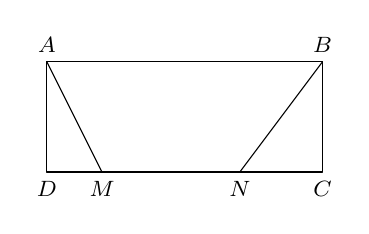
\begin{tikzpicture}[scale=0.7,font=\footnotesize,line join=round,line cap=round,>=stealth]
			\draw (0,0) rectangle  (5,-2);
			\path 
				(0,0) node[above]{$A$} 
				(5,0) node[above]{$B$} 
				 (5,-2) node[below]{$C$}
				 (3.5,-2) node[below]{$N$}
				 (1,-2) node[below]{$M$}
				 (0,-2) node[below]{$D$};
			\draw (0,0)  -- (1,-2);
			\draw (5,0) -- (3.5,-2); 
		\end{tikzpicture}
		} 
		\noindent Áp dụng bất đẳng thức $\sqrt{a^2+b^2}+\sqrt{c^2+d^2}  \ge \sqrt{(a+c)^2+(b+d)^2}$, ta có
		$$t \ge \dfrac{\sqrt{20^2+(m+n)^2}}{20}+\dfrac{70-(m+n)}{40},$$ 
		 dấu \lq \lq $=$\rq \rq \, xảy ra khi và chỉ khi $m=n$.\\
		Đặt $m+n=x$, xét hàm $f(x)=\dfrac{\sqrt{400+x^2}}{20}+\dfrac{70-x}{40},~x \in (0,70]$.\\ 
		Ta có $f'(x)=\dfrac{x}{20\sqrt{400+x^2}}-\dfrac{1}{40},~x \in  [0,70]$.
		\[f'(x)=0 \Leftrightarrow \sqrt{400+x^2}=2x \Leftrightarrow  x=\dfrac{20}{\sqrt{3}}.\]
		Bảng biến thiên  của $f(x)$
		\begin{center}
			
\begin{tikzpicture}[scale=1,font=\footnotesize,line join=round,line cap=round,>=stealth]
				 \tkzTabInit[nocadre=false,lgt=1.2,espcl=2.5,deltacl=0.6]
					{$x$/1,$f'(x)$/0.6,$f  (x)$/2}
					 {$0$,$\dfrac{20}{\sqrt{3}}$,$70$}
				 \tkzTabLine{,-,0,+,}
				 \tkzTabVar{+/$\dfrac{11}{4}$,-/$\dfrac{2\sqrt{3}+7}{4}$,+/$\dfrac{\sqrt{50}}{2}$}
			\end{tikzpicture}
		\end{center}
		$\Rightarrow$ giá trị nhỏ nhất của $f(x)$ là $f\left(\dfrac{20}{\sqrt{3}}\right)=\dfrac{2\sqrt{3}+7}{4}$.\\ 
		 Vậy thời gian ngắn nhất là $\dfrac{2\sqrt{3}+7}{4}$ khi $m=n=\dfrac{x}{2}=\dfrac{10}{\sqrt{3}}$.
	 }
\end{ex}

% nguồn: Phan1_Lop_12_Dai_so_Chuong_1
\begin{ex}%[2D1C3-6]%[ma:598a412c]
	\immini 
	{Hình vẽ bên dưới mô tả đoạn đường đi vào gara ô tô nhà cô Lan. Đoạn đường đầu tiên có chiều rộng bằng $x$ m, đoạn đường thẳng vào cổng GARA có chiều rộng $2{,}6$ m. Biết kích thước xe ô tô là $5 \ \text{ m} \ \times 1{,}9 \ \text{ m}$. Để tính toán và thiết kế đường đi cho ô tô  người ta coi ô tô như một khối hộp chữ nhật có kích thước chiều dài $5$ m, chiều rộng $1{,}9$ m. Hỏi chiều rộng nhỏ nhất của đoạn đường đầu tiên gần nhất với giá trị nào trong các giá trị bên dưới để ô tô có thể đi vào GARA được?
	 \choice
		{\True $x  = 3{,}7$ m}
		 {$x = 2{,}6$ m}
		{$x  = 3{,}55$ m}
		{$x =  4{,}27$ m}
		 }
		{\begin{tikzpicture}[>=stealth,scale=0.3]
		\def\xehoi{ 
		 \tikz{
		\path[fill] (1.78,5.03) -- (1.65,5.08).. controls +(87:0.2) and  +(-90:0.2)..
			(1.71,5.57) --  (1.71,7.21) -- (1.71,7.21) --
			(1.71,7.21).. controls +(90:0.5)  and +(-3:0.2)..
			(1.03,7.95) -- (-1.03,7.95).. controls +(180:0.2) and  +(90:0.5)..
			(-1.72,7.21) -- (-1.72,7.21) --  (-1.72,5.57).. controls +(-90:0.2) and +(93:0.2)..
			 (-1.65,5.08).. controls +(-163:0.1) and +(85:0.1)..
			(-1.85,4.91) --  (-1.85,4.83).. controls +(-85:0.1) and +(-157:0.1)..
			(-1.65,4.82) -- (-1.65,1.47).. controls +(-90:0.1) and  +(72:0.1)..
			 (-1.68,1.29).. controls +(-107:0.2) and +(90:0.2)..
			 (-1.72,0.68) -- (-1.72,0.68) -- (-1.72,0.68).. controls +(-90:0.3) and +(153:0.2)..
			(-1.38,0.09).. controls  +(-29:0.1) and +(180:0.1)..
			(-1.08,0) -- (-1.08,0) -- (1.08,0) -- (1.08,0).. controls +(-0:0.1) and +(-156:0.1).. 
			(1.38,0.09).. controls +(27:0.2) and  +(-90:0.3)..
			(1.72,0.68) -- (1.72,0.68)  -- (1.72,0.68) --
			(1.72,1.1).. controls  +(90:0.2) and +(-90:0.2)..
			(1.65,1.47) -- (1.65,4.82) -- (1.77,4.76)..  controls +(-6:0.1) and +(-90:0.1)..
			(1.85,4.91)..  controls +(90:0) and +(-27:0)..
			(1.78,5.03)  -- cycle
			(1.32,5.43) -- (1.15,5)..  controls +(-110:0.2) and +(0:0.2)..
			(0.72,4.69) --  (-0.73,4.69).. controls +(180:0.2) and +(-70:0.2)..
			(-1.15,5)  -- (-1.32,5.43).. controls +(17:0.9) and +(163:0.9)..
			 (1.32,5.43) -- cycle
			(-1.45,5.17) -- (-1.07,4.61) -- (-1.07,3.07) -- (-1.45,3.04)  -- cycle
			(-1.45,1.33) -- (-1.45,2.86) --  (-1.07,2.99) -- (-1.06,1.91) -- cycle
			(-1.31,1.07) -- (-1.14,1.48).. controls  +(69:0.3) and +(180:0.3)..
			(-0.54,1.91) -- (0.59,1.91).. controls +(0:0.2)  and +(111:0.2)..
			(1.12,1.53)  -- (1.31,1.07).. controls +(-169:0.9) and +(-11:0.9)..
			 (-1.31,1.07) -- cycle
			(1.45,1.33) -- (1.05,1.91) -- (1.07,2.99)  -- (1.45,2.86) -- cycle
			 (1.45,3.04) -- (1.07,3.07) -- (1.07,4.61) -- (1.45,5.17) -- cycle;
		 }
		 }
		 \draw[pattern=north west lines]
			(-12,0)--(0,0)--(0,9)--(-0.5,9)--(-0.5,0.5)--(-12,0.5)--cycle 
			(-12,-4)--(3,-4)--(3,9)--(3.5,9)--(3.5,-4.5)--(-12,-4.5)--cycle; 
		\path (-7,-2)  node[rotate=-90]{\resizebox{0.7cm}{!}{\xehoi}};
		 \path (-0.13,-1.6) node[rotate=-65]{\resizebox{0.7cm}{!}{\xehoi}};
		\path  (1.5,5) node{\resizebox{0.7cm}{!}{\xehoi}};
		\draw[blue,|<->|] (-12,0)--(-12,-4)  node[pos=0.5,left]{$x$(m)};
		 \draw[blue,|<->|] (0,9)--(3,9) node[pos=0.5,above]{$2{,}6$(m)};
	\end{tikzpicture}
		} 
	\loigiai{ 
	 \immini
		{Chọn hệ trục $Oxy$ như hình  vẽ.\\ Khi đó $M(-2{,}6; x)$.\\
		Gọi $B(-a; 0)$.  \\
		Suy ra  $A\left(0, \sqrt{25 - a^2} \right)$.\\
		Phương trình  $$AB\colon \ \dfrac{x}{-a} + \dfrac{y}{\sqrt{25 - a^2}} - 1 = 0.$$
		 Do $CD \parallel AB$ nên phương trình $$CD\colon -\dfrac{x}{a} + \dfrac{y}{\sqrt{25 - a^2}} - T = 0.$$
		 }
		{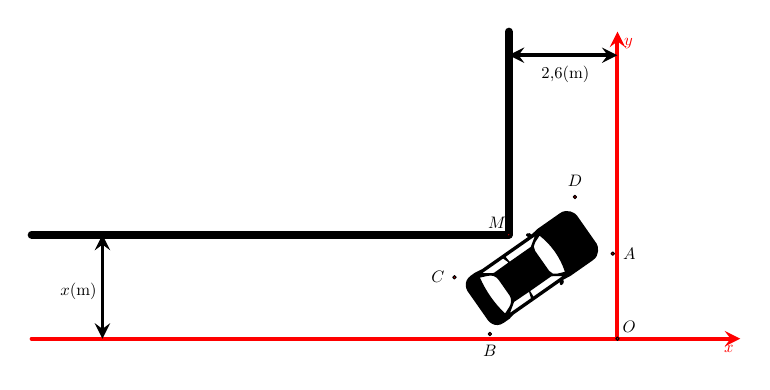
\begin{tikzpicture}[line join=round,line cap=round,scale=0.6,transform shape,>=stealth]
		 \def\xehoi{
		\tikz{ 
		\path[fill]  (1.78,5.03) -- (1.65,5.08).. controls +(87:0.2) and +(-90:0.2)..
			(1.71,5.57) --  (1.71,7.21) -- (1.71,7.21) --
			(1.71,7.21).. controls  +(90:0.5) and +(-3:0.2)..
			(1.03,7.95)  -- (-1.03,7.95).. controls +(180:0.2) and +(90:0.5)..
			(-1.72,7.21) -- (-1.72,7.21)  -- (-1.72,5.57).. controls +(-90:0.2) and +(93:0.2)..
			(-1.65,5.08).. controls +(-163:0.1) and +(85:0.1).. 
			(-1.85,4.91) -- (-1.85,4.83).. controls +(-85:0.1) and +(-157:0.1).. 
			 (-1.65,4.82) -- (-1.65,1.47).. controls +(-90:0.1) and +(72:0.1)..
			(-1.68,1.29).. controls  +(-107:0.2) and +(90:0.2)..
			(-1.72,0.68) --  (-1.72,0.68) -- (-1.72,0.68).. controls +(-90:0.3) and +(153:0.2)..
			(-1.38,0.09)..  controls +(-29:0.1) and +(180:0.1)..
			(-1.08,0) -- (-1.08,0) -- (1.08,0) -- (1.08,0).. controls +(-0:0.1) and  +(-156:0.1)..
			(1.38,0.09)..  controls +(27:0.2) and +(-90:0.3)..
			(1.72,0.68) --  (1.72,0.68) -- (1.72,0.68) --
			(1.72,1.1)..  controls +(90:0.2) and +(-90:0.2)..
			(1.65,1.47) --  (1.65,4.82) -- (1.77,4.76).. controls +(-6:0.1) and +(-90:0.1)..
			(1.85,4.91)..  controls +(90:0) and +(-27:0)..
			(1.78,5.03) -- cycle 
			(1.32,5.43) -- (1.15,5).. controls  +(-110:0.2) and +(0:0.2)..
			(0.72,4.69) -- (-0.73,4.69).. controls  +(180:0.2) and +(-70:0.2)..
			(-1.15,5) --  (-1.32,5.43).. controls +(17:0.9) and +(163:0.9)..
			(1.32,5.43)  -- cycle
			(-1.45,5.17) --  (-1.07,4.61) -- (-1.07,3.07) -- (-1.45,3.04) -- cycle
			(-1.45,1.33) -- (-1.45,2.86) -- (-1.07,2.99) -- (-1.06,1.91) --  cycle
			(-1.31,1.07) -- (-1.14,1.48).. controls +(69:0.3)  and +(180:0.3)..
			(-0.54,1.91) --  (0.59,1.91).. controls +(0:0.2) and +(111:0.2)..
			(1.12,1.53) -- (1.31,1.07)..  controls +(-169:0.9) and +(-11:0.9)..
			(-1.31,1.07) --  cycle
			(1.45,1.33) -- (1.05,1.91)  -- (1.07,2.99) -- (1.45,2.86) -- cycle
			(1.45,3.04) -- (1.07,3.07) -- (1.07,4.61)  -- (1.45,5.17) -- cycle;
		} 
		 }
		\path (5.6,-2.5)  node[rotate=-55]{\resizebox{1.4cm}{!}{\xehoi}};
		 \draw[line width=1mm] (5.1,2.5)--(5.1,-1.8)--(-5,-1.8);
		\draw[red,->,line width=0.5mm] (-5,-4)--(10,-4)  node[below left]{$x$};
		\draw[red,->,line width=0.5mm] (7.4,-4)--(7.4,2.5) node[below right]{$y$}; 
		 \draw[line width=.5mm,<->] (-3.5,-1.8)--(-3.5,-4);
		 \draw[line width=.5mm,<->] (5.1,2)--(7.4,2);
		\node[left] at  (-3.5,-3){$x$(m)};
		\node  at (6.3,1.6){$2{,}6$(m)};
		\path (7.4,-4)  coordinate (O)
			 (4.7,-3.9) coordinate (B)
			(7.3,-2.2)  coordinate (A)
			 (6.5,-1) coordinate (D)
			(3.95,-2.7)  coordinate (C)
			(5.1,-1.8) coordinate  (M);
		 \foreach \d/\g in {B/-90,A/0,D/90,C/180,O/45,M/135}{
			\draw[fill=red](\d) circle  (1pt) +(\g:.35) node{$\d$};}
	\end{tikzpicture}
		 }\noindent
		Mà khoảng cách giữa $AB$ và $CD$ bằng $1{,}9$ m  nên
		$$\dfrac{\left|T - 1 \right|}{\sqrt{\left(\dfrac{1}{a}\right)^2 + \left( \dfrac{1}{\sqrt{25 - a^2}} \right)^2}} =  1{,}9 \Rightarrow T = 1 + \dfrac{9{,}5}{a\sqrt{25 - a^2}}.$$
		Điều kiện để ô  tô đi qua được là $M$, $O$ nằm khác phía đối với bờ là đường thẳng $CD$.
		 Suy ra
		$$\dfrac{-2{,}6}{-a} + \dfrac{x}{\sqrt{25 - a^2}} - 1 - \dfrac{9{,}5}{a\sqrt{25 - a^2}} \ge 0 \Leftrightarrow x \ge \sqrt {25 - a^2} +  \dfrac{9{,}5}{a} - \dfrac{2{,}6\sqrt{25 - a^2}}{a}.$$
		Sử dụng chức năng TABLE trong  máy tính
		$f(X)  = \sqrt{25 - X^2} + \dfrac{9{,}5}{X} - \dfrac{2{,}6\sqrt{25 - X^2}}{X}$ \break với STEP = $\dfrac{5}{29}$; START = $0$; END = $5$.\\
		Thấy giá  trị lớn nhất của $f(X) = \sqrt {25-X^2} + \dfrac{9{,}5}{X} - \dfrac{2{,}6\sqrt {25-{X^2}}}{X}$ xấp xỉ $3{,}698$.\\
		Vậy chiều rộng nhỏ nhất của  đoạn đường đầu tiên gần nhất với giá trị $ x=3{,}7$ m.
	} 
\end{ex}

% nguồn: Phan1_Lop_12_Dai_so_Chuong_1
\begin{ex}%[2D1C3-6]%[ma:f01b2956]
	 \immini
	{Một màn ảnh hình chữ nhật cao $1{,}4$ mét và đặt ở độ cao $1{,}8$ m so với tầm mắt, tính từ đầu mép dưới của màn hình (mép dưới màn hình là điểm $B$, mép trên màn hình là điểm $C$, tầm mắt là điểm $A$ và vị trí người đó phải cách màn ảnh là điểm $O$ như hình vẽ bên). Để nhìn rõ nhất người đó phải cách  màn ảnh khoảng bao nhiêm mét, biết rằng góc $\widehat{BOC}$ là góc nhọn.
	\choice 
		{\True $AO=2{,}4$ m} 
		{$AO=2$ m} 
		 {$AO=2{,}6$ m}
		{$AO=3$  m}
		} 
		{\begin{tikzpicture}[join = round,cap = round,font = \small,scale = 0.8]
		 \path
			(0,0) coordinate (A) 
			+(0:5) coordinate (O) 
			+(90:3)  coordinate (C)
			 +(90:1.8) coordinate (B);
		\draw (A)--(O)--(C)--(B); 
		\draw[dashed]  (A)--(B);
		\foreach  \x/\g in {A/180,O/0,C/90,B/180}
		\fill (\x) circle (1.5pt) 
			 +(\g:3mm) node{$\x$};
		 \path (-0.5,0.8) node{$1{,}8$};
		 \path (-0.5,2.4) node{$1{,}4$};
	\end{tikzpicture}
		} 
	\loigiai{ 
		Đặt độ dài cạnh $AO = x$  cm, ($x > 0$).\\
		Suy ra $BO = \sqrt {3{,}24 + x^2}$, $CO  = \sqrt{10{,}24 + x^2}$.\\
		Áp dụng định lí cosintrong $\triangle OBC$  ta có
		\allowdisplaybreaks 
		\begin{eqnarray*}
			\cos \widehat{BOC} 
			&=& \dfrac{OB^2 + OC^2 - BC^2}{2  \cdot OB \cdot OC}\\
			&=& \dfrac{\left(3{,}24 + x^2\right) + \left(10{,}24 + x^2 \right) - 1{,}96}{2\sqrt{\left(3{,}24 +  x^2\right)\left(10{,}24 + x^2 \right)}}\\
			&=& \dfrac{5{,}76 + x^2}{\sqrt{\left(3{,}24 + x^2 \right)(10{,}24 +  x^2)}}.
		\end{eqnarray*}
		Xét hàm số $F(x) = \dfrac{5{,}76 + x^2}{\sqrt{\left(3{,}24 + x^2 \right)(  10{,}24 + x^2)}}$ với $x > 0$.\\
		Đặt $t = 3{,}24 + x^2$ với $t > 3{,}24$. Suy ra $F(t) = \dfrac{t + \dfrac{63}{25}}{\sqrt{t(t + 7)}} = \dfrac{25t + 63}{25\sqrt{t(t +  7)}}$.\\
		Ta  có
		 \allowdisplaybreaks
		\begin{eqnarray*}
			F'(t) 
			&=& \left(\dfrac{25t +  63}{25\sqrt{t(t + 7)}} \right)'\\
			&=& \dfrac{1}{25} \cdot \dfrac{50\left(t^2 + 7t \right) - \left(25t + 63  \right)\left( 2t + 7 \right)}{2t(t + 7)\sqrt{t(t + 7)}}\\
			&=& \dfrac{1}{25} \cdot  \dfrac{25\sqrt{t(t + 7)} - (25t + 63) \cdot \dfrac{2t + 7}{2\sqrt{t(t + 7)}}}{t(t + 7)}\\
			&=&  \dfrac{1}{25} \cdot \dfrac{49t - 441}{2t(t + 7)\sqrt{t(t + 7)}}.
		\end{eqnarray*}
		Khi đó $F'(t)  = 0 \Leftrightarrow t = 9$.\\
		Bảng biến thiên 
		\begin{center}
			
\begin{tikzpicture}
				 \tkzTabInit[lgt=1.2,espcl=4]
					{$t$/1,$F'(t)$/1,$F (t)$/2} 
					{$3{,}24$,$9$,$+\infty$} 
				 \tkzTabLine{,-,$0$,+,}
				 \tkzTabVar{+/,-/$F_{min}$,+/}
			\end{tikzpicture}
		\end{center}
		Theo cách đặt ta có $3{,}24 + x^2 = 9  \Leftrightarrow x^2 = \dfrac{144}{25} \Leftrightarrow x = 2{,}4$ m.\\
		Vậy để nhìn  rõ nhất thì $AO = 2{,}4$ m.
	 }
\end{ex}

% nguồn: Phan1_Lop_12_Dai_so_Chuong_1
\begin{ex}%[2D1C3-6]%[ma:291ebecc]
	Để thiết kế một chiếc  bể cá hình chữ nhật có chiều cao là $60$ cm thể tích là $96\,000$ cm$^3$, người thợ dùng loại kính để sử dụng làm mặt bên có giá thành $70\,000$ đồng/m$^2$ và loại kính để làm mặt đáy có giá thành là $100\,000$ đồng/m$^2$. Chi phí thấp nhất để hoàn thành bể cá là
	\choice 
		{$83\,200\,000$  đồng}
		{$382\,000$ đồng} 
		{\True $83\,200$ đồng} 
		{$8\,320\,000$  đồng}
	\loigiai{ 
		Diện tích của đáy hộp là $S = \dfrac{V}{h} = \dfrac{96\,000}{60} = 1\,600 $  cm$^2 = 0{,}16$ m$^2$.\\
		 Gọi chiều dài cạnh đáy của hộp là $x$ m ($x > 0$), chiều rộng của hộp là $\dfrac{0{,}16}{x}$ m.\\
		Gọi $F( x)$ là hàm chi phí để làm để  cá.\\
		Chi phí để hoàn thành  bể cá là
		\allowdisplaybreaks 
		\begin{eqnarray*}
			F(x) 
			&=& 0{,}16 \cdot 100\,000 + 2\cdot 0{,}6x \cdot 70\,000 + 2 \cdot 0{,}6 \cdot \dfrac{0{,}16}{x}  \cdot 70\,000\\
			&=& 16\,000 + 48\,000x + \dfrac{13\,440}{x}. 
		\end{eqnarray*}
		Xét hàm số $F(x) = 16\,000 + 48\,000x + \dfrac{13\,440}{x}$ với $x  > 0$.\\
		Ta có $F'(x)  = 84\,000 - \dfrac{13\,440}{x^2}$.\\
		Khi đó  $F'(x) = 0 \Leftrightarrow 84\,000 - \dfrac{13\,440}{x^2} = 0 \Leftrightarrow x = 0{,}4$.\\
		 Bảng biến thiên
		\begin{center}
			
\begin{tikzpicture}
				\tkzTabInit[lgt=1.2,espcl=4] 
					 {$x$/1,$F'(x)$/1,$F (x)$/2}
					{$0$,$0{,}4$,$+\infty$} 
				\tkzTabLine{,-,z,+,} 
				 \tkzTabVar{+/,-/$F_{\min}$,+/}
			\end{tikzpicture}
		\end{center}
		Vậy chi phí thấp nhất để hoàn thành bể cá  là $F(0{,}4)=83\,200$ đồng.
	 }
\end{ex}

% nguồn: Phan1_Lop_12_Dai_so_Chuong_1
\begin{ex}%[2D1C3-6]%[ma:679bdd8d]
	Ông Nam cần xây dựng một bể nước mưa có thể tích $V = 8$ m$^3$ dạng hình hộp chữ nhật với chiều dài gấp $\dfrac{4}{3}$ lần chiều rộng, đáy và nắp đổ bê tông, cốt thép; xung quanh xây bằng gạch và xi măng. Biết rằng chi phí trung bình là $980\,000$ đồng/m$^2$ và ở nắp để hở một khoảng hình vuông có diện tích bằng $\dfrac{2}{9}$  diện tích nắp bể. Tính chi phí thấp nhất mà ông Nam phải chi trả (làm tròn đến hàng nghìn đồng).
	\choice 
		{$22\,770\,000$ đồng} 
		{\True $27\,657\,000$  đồng}
		{$20\,965\,000$  đồng}
		{$23\,235\,000$  đồng}
	\loigiai{ 
		Gọi chiều rộng của bể là  $3x$ m ($x>0$).\\
		Ta có chiều dài bể là $4x$ m và chiều cao của bể là $\dfrac{2}{3x^2}$ m.\\ 
		 Khi đó tổng diện tích bề mặt xây là
		\allowdisplaybreaks 
		\begin{eqnarray*}
			T 
			&=& (3x + 4x) \cdot 2 \cdot \dfrac{2}{3x^2} + 2 \cdot 3x \cdot 4x -  \dfrac{2}{9} \cdot 3x \cdot 4x\\
			&\geq& 2\sqrt{\dfrac{28}{3x^2} \cdot \dfrac{64x^2}{3}}\\ 
			&=&  \dfrac{32\sqrt{7}}{3} \ \text{ m}^2.
		\end{eqnarray*}
		Chi phí $C$ xây dựng là $C = T \cdot 980\,000 \ge \dfrac{32\sqrt{7}}{3} \cdot 980\,000  \approx 27\,657\,000$ (đồng).
	 }
\end{ex}

% nguồn: Phan1_Lop_12_Dai_so_Chuong_1
\begin{ex}%[2D1C3-6]%[ma:2be5bede]
	 \immini
	{Dùng một dây thép dài $60$ m uốn thành một khung có dạng như hình vẽ. Biết phần dưới là hình  chữ nhật và phía trên là một tam giác đều. Diện tích lớn nhất của khung có giá trị bằng
	 \choice
		{\True $\dfrac{900}{6 - \sqrt{3}}$  m$^2$}
		{$\dfrac{1\,200}{6 - \sqrt{3}}$ m$^2$} 
		{$\dfrac{700}{3  + \sqrt{3}}$ m$^2$}
		{$\dfrac{600}{3 - \sqrt{3}}$ m$^2$} 
		 }
		{\begin{tikzpicture}[join = round,cap = round,font = \small,scale = 0.6]
		\path 
			(0:0) coordinate  (D)
			+(0:6) coordinate (C) 
			+(90:4) coordinate  (A)
			(6,4) coordinate (B) 
			 (3,7) coordinate (E)
			($(C)!.5!(D)$)  coordinate (M);
		 \draw
			 (A)--(D)--(C)--(B)--(E)--cycle;
		\draw[dashed] (A)--(B) 
			 (M)--(E);
	\end{tikzpicture}
		} 
	 \loigiai{
	 \immini
		{Gọi hai cạnh của hình chữ nhật là $x$ (m) và $y$ (m) như hình vẽ  ($x>0$, $y>0$).\\
		Khi đó chu vi của khung là $(x + 2y) + 2x = 60 \Leftrightarrow y = 30 -  \dfrac{3}{2}x$.\\
		Suy ra diện tích  của khung là
		$$S = xy + \dfrac{x^2\sqrt{3}}{4} = x \left( 30 -  1{,}5x \right) + \dfrac{x^2\sqrt{3}}{4} = \dfrac{\sqrt{3} - 6}{4}x^2 + 30x = f(x).$$
		Xét hàm số $f(x) = \dfrac{\sqrt{3} - 6}{4}x^2  + 30x$ với $x > 0$.\\
		Ta có $f'(x) = \dfrac{\sqrt{3} -  6}{2}x + 30$.\\
		Khi đó  $f'(x) = 0 \Leftrightarrow x = \dfrac{60}{6 - \sqrt{3}}$.
		 }
		{\begin{tikzpicture}[join = round,cap = round,font = \small,scale = 0.6]
		\path 
			(0:0)  coordinate (D)
			+(0:6) coordinate (C) 
			+(90:4) coordinate (A) 
			(6,4) coordinate (B) 
			(3,7) coordinate  (E)
			($(C)!.5!(D)$) coordinate (M); 
		 \draw
			(A)--(D)--(C)--(B)--(E)--cycle; 
		\draw[dashed]  (A)--(B)
			 (M)--(E);
		\path  (3,-0.5) node{$x$};
		 \path (6.5,2) node{$y$};
	\end{tikzpicture}
		}\noindent 
		 Bảng biến thiên
		\begin{center}
			
\begin{tikzpicture}
				 \tkzTabInit[lgt=1.2,espcl=4]
					 {$x$/1,$f'(x)$/1,$f (x)$/2}
					{$0$,$\dfrac{60}{6 -  \sqrt{3}}$,$+\infty$}
				\tkzTabLine{,+,$0$,-,} 
				\tkzTabVar{-/,+/$S_{\max}$,-/} 
			\end{tikzpicture}
		\end{center}
		Vậy $S_{\max} = \max f(x) = f\left(\dfrac{60}{6 - \sqrt{3}} \right) = \dfrac{900}{6 -  \sqrt{3}}$ m$^2$.
	 }
\end{ex}

% nguồn: Phan1_Lop_12_Dai_so_Chuong_1
\begin{ex}%[2D1C3-6]%[ma:1188a373]
	Trong một bài thực hành huấn luyện quân sự có một tình huống chiến sĩ phải bơi qua sông để tấn công mục tiêu ở ngay phía bờ  bên kia sông. Biết rằng lòng sông rộng $100$ m và vận tốc bơi của chiến sĩ bằng một phần ba vận tốc chạy trên bộ. Hãy cho biết chiến sỹ phải bơi bao nhiêu mét để đến được mục tiêu nhanh nhất? Biết dòng sông là thẳng, mục tiêu cách chiến sỹ $1$ km theo đường chim bay và chiến sỹ cách bờ bên kia $100$ m.
	\choice 
		{$\dfrac{200\sqrt{2}}{3}$} 
		{\True $60\sqrt{5}$} 
		{$\dfrac{200\sqrt{3}}{3}$} 
		 {$75\sqrt{2}$}
	\loigiai{ 
	\immini 
		{Gọi vận tốc  của chiến sĩ khi bơi là $a$ (m/s) với $a>0$.\\
		Suy ra vận tốc của chiến sĩ khi  chạy bộ là $3a$ (m/s).\\
		Ta có hình vẽ, khi đó chiến sĩ ở vị trí $A$,  mục tiêu ở vị trí $C$.\\
		Quãng đường chiến sĩ phải bơi là $AD$, quãng đường chiến sĩ phải chạy bộ là  $DC$.
		 }
		{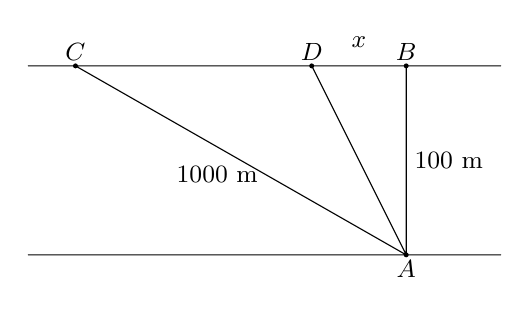
\begin{tikzpicture}[join = round,cap = round,font = \small,scale = 0.6]
		\path 
			(0,0) coordinate  (B)
			(-2,0) coordinate  (D)
			(-7,0) coordinate (C) 
			(0,-4) coordinate (A) 
			(2,0) coordinate  (E)
			 (-8,0) coordinate (F)
			 (2,-4) coordinate (H)
			(-8,-4) coordinate (G); 
		\draw  (E)--(F)
			(H)--(G) 
			 (B)--(A)--(D)
			 (A)--(C);
		\foreach \x/\g  in {C/90,A/-90,B/90,D/90}
		\fill (\x) circle (1.5pt) 
			+(\g:3mm) node  {$\x$};
		\path (0.9,-2) node{$100$  m};
		\path  (-4,-2.3) node{$1000$ m};
		 \path (-1,0.5) node{$x$};
	\end{tikzpicture}
		 }\noindent
		Ta  có $BC = \sqrt{AC^2 - AB^2} = \sqrt{1000^2 - 100^2} = 300\sqrt{11}$ (m).\\
		Đặt $BD = x$ (m) với $0  < x < 300\sqrt{11}$.\\
		Suy ra  quãng đường chiến sĩ phải bơi là $$AD = \sqrt{AB^2 + BD^2} = \sqrt{x^2 + 100^2} \text{ (m)}.$$
		Quãng đường chiến sĩ phải chạy bộ là $CD =  BC - BD = 300\sqrt{11} - x$ (m).\\
		Vậy  thời gian chiến sĩ đến được mục tiêu là
		\allowdisplaybreaks 
		\begin{eqnarray*}
			 t
			&=& \dfrac{AD}{a} + \dfrac{DC}{3a}\\ 
			&=& \dfrac{\sqrt{x^2 + 100^2}}{a} + \dfrac{300\sqrt{11} -  x}{3a}\\
			&=& \dfrac{1}{3a}\left(3\sqrt{x^2  + 100^2} + 300\sqrt{11}-x\right).
		\end{eqnarray*}
		Xét hàm số $f(x) = 3\sqrt{x^2 + 100^2} - x  + 300\sqrt{11}$ trên $\left(0; 300\sqrt{11}\right)$.\\
		Ta có $f'(x) = \dfrac{3x}{2\sqrt{x^2+100^2}} - 1 = \dfrac{3x - 2\sqrt{x^2 + 100^2}}{2\sqrt{x^2  + 100^2}}$.\\
		 Khi đó
		\begin{eqnarray*}
			f'(x) =  0 &\Leftrightarrow& 3x = 2\sqrt{x^2+100^2}\\
			& \Leftrightarrow& 9x^2 = 4x^2 +  4 \cdot 100^2 \\
			&\Leftrightarrow& x^2 = \dfrac{4}{5} \cdot 100^2\\ 
			& \Leftrightarrow& \hoac{&x= -40\sqrt{5}\\&x= 40\sqrt{5}.} 
		\end{eqnarray*}
		Vì $x= -40\sqrt{5} \notin \left(0; 300\sqrt{11}\right)$ và $x= 40\sqrt{5} \in \left(0; 300\sqrt{11}\right)$ nên  ta có bảng biến thiên sau
		\begin{center}
			\begin{center}
				
\begin{tikzpicture}
					\tkzTabInit[lgt=1.5,espcl=4,nocadre=true,] 
						{$x$/1,$f'(x)$/1,$f (x)$/2} 
						{$0$,$40\sqrt{5}$,$\makebox[0pt][r]{$300\sqrt{11}$}$} 
					 \tkzTabLine{,-,$0$,+,}
					\tkzTabVar{+/,-/$f (40\sqrt{5})$,+/} 
				\end{tikzpicture}
			\end{center}
		\end{center}
		Quãng đường bơi mà chiến sĩ  phải bơi để đến được mục tiêu nhanh nhất là
		$$AD  = \sqrt{x^2+100^2} = \sqrt{\dfrac{4}{5} \cdot 100^2 + 100^2} = \sqrt{\dfrac{9}{5} \cdot 100^2} = 60\sqrt{5} \ \text{ (m)}.$$
	 }
\end{ex}

% nguồn: Phan1_Lop_12_Dai_so_Chuong_1
\begin{ex}%[2D1C3-6]%[ma:69c9155b]
	 \immini
	{Cho hình vuông $ABCD$ có cạnh bằng $4$, chính giữa có một hình vuông đồng tâm với $ABCD$ như hình vẽ bên. Biết rằng bốn tam giác là bốn tam giác cân. Hỏi tổng diện tích của hình vuông ở giữa và bốn tam giác cân nhỏ nhất bằng bao  nhiêu?
	\choice 
		 {$\dfrac{19}{3}$}
		{$\dfrac{17}{3}$} 
		 {\True $\dfrac{16}{3}$}
		{$\dfrac{14}{3}$} 
		 }
		{\begin{tikzpicture}[join = round,cap = round,font = \small,scale = 0.8]
		\def\canh{4} 
		 \path
			(0:0)  coordinate (A)
			++(0:\canh) coordinate (B) 
			++(-90:\canh) coordinate  (C)
			($(A)+(C)-(B)$) coordinate (D) 
			($(A)!.25!(B)$) coordinate  (A1)
			($(A)!.75!(B)$) coordinate  (A2)
			($(B)!.25!(C)$) coordinate (B1) 
			($(B)!.75!(C)$) coordinate  (B2)
			($(C)!.25!(D)$) coordinate  (C1)
			($(C)!.75!(D)$) coordinate (C2) 
			($(D)!.25!(A)$) coordinate (D1) 
			($(D)!.75!(A)$) coordinate (D2) 
			 (intersection of A1--B2 and A2--D1) coordinate (M)
			(intersection of A1--B2 and  B1--C2) coordinate (N)
			(intersection of C1--D2 and B1--C2)  coordinate (P)
			(intersection of A2--D1 and C1--D2) coordinate (Q); 
		\draw (A)--(B)--(C)--(D)--cycle 
			 (A1)--(B2)
			 (B1)--(C2)
			(A2)--(D1) 
			(C1)--(D2); 
		\fill[gray!50,opacity=0.5]  (M)--(A1)--(A2)--(M)--(N)--(B1)--(B2)--(N)--(P)--(C1)--(C2)--(P)--(Q)--(D1)--(D2)--(Q);
		 \foreach \x/\g in {A/90,B/90,C/-90,D/-90}
		\fill (\x) circle (1.5pt) 
			+(\g:3mm) node  {$\x$};
	\end{tikzpicture}
		 }
	\loigiai{ 
	\immini 
		{Đặt $AM = x$ với $0 < x < 4$. Suy  ra $ME = 4 - 2x$.\\
		Ta có $$2MQ^2= (4 - 2x)^2 \Leftrightarrow MQ^2 = 2(2  - x)^2 \Leftrightarrow MQ = \sqrt{2(2 - x)}.$$
		Gọi $S$ tổng diện tích của hình vuông ở giữa và bốn tam giác  cân nhỏ.\\
		Khi  đó $$S = 4 \cdot \dfrac{MQ^2}{2} + PQ^2 = 2MQ^2 + MN^2 = (4 - 2x)^2 + \left(x\sqrt{2} \right)^2 = 6x^2 - 16x + 16.$$
		 Ta có $S' = 12x -16$.\\
		Khi đó $S' =  0 \Leftrightarrow x = \dfrac{4}{3}$.
		} 
		{\begin{tikzpicture}[join = round,cap = round,font = \small,scale = 0.8]
		 \def\canh{4}
		\path 
			(0:0) coordinate (A) 
			++(0:\canh)  coordinate (B)
			++(-90:\canh) coordinate (C) 
			($(A)+(C)-(B)$) coordinate  (D)
			($(A)!.25!(B)$) coordinate  (M)
			 ($(A)!.75!(B)$) coordinate (E)
			($(B)!.25!(C)$) coordinate (B1) 
			 ($(B)!.75!(C)$) coordinate (B2)
			($(C)!.25!(D)$) coordinate (C1) 
			($(C)!.75!(D)$) coordinate (C2) 
			 ($(D)!.25!(A)$) coordinate (D1)
			($(D)!.75!(A)$) coordinate (N) 
			(intersection  of M--B2 and E--D1) coordinate (Q)
			(intersection of  M--B2 and B1--C2) coordinate (M2)
			(intersection of C1--N and B1--C2) coordinate (M3) 
			(intersection of  E--D1 and C1--N) coordinate (P);
		 \draw (A)--(B)--(C)--(D)--cycle
			(M)--(B2) 
			 (B1)--(C2)
			 (E)--(D1)
			 (C1)--(N);
		 \fill[gray!50,opacity=0.5] (Q)--(M)--(A2)--(Q)--(M2)--(B1)--(B2)--(M2)--(M3)--(C1)--(C2)--(M3)--(P)--(D1)--(N)--(P);
		 \foreach \x/\g in {A/180,B/90,C/-90,D/-90,E/-70,M/-130,P/-90,Q/90,N/150}
		\fill (\x) circle  (1.5pt)
			+(\g:3mm)  node {$\x$};
		\path (0.4,0.3) node{$x$}; 
		\path (2.0,0.3) node{$4  - 2x$};
	\end{tikzpicture}
		}\noindent 
		Bảng biến thiên 
		\begin{center}
			
\begin{tikzpicture}
				 \tkzTabInit[lgt=1.2,espcl=4,deltacl=0.9]
					{$t$/1,$F'(t)$/1,$F (t)$/2} 
					{$0$,$\dfrac{4}{3}$,$4$} 
				\tkzTabLine{,-,$0$,+,} 
				 \tkzTabVar{+/,-/$\dfrac{16}{3}$,+/}
			\end{tikzpicture}
		\end{center}
		Vậy  $S_{\min } = \dfrac{16}{3}$.
	} 
\end{ex}


%%%%%%%%%%%%%%%% ĐÚNG/SAI %%%%%%%%%%%%%%%%

% nguồn: Phan1_Lop_12_Dai_so_Chuong_1
\begin{ex}%[2D1H3-6]%[ma:bd557383]
	Người ta bơm xăng vào bình xăng của một xe ô tô. Biết rằng thể tích $V$ (lít) của  lượng xăng trong bình xăng được tính theo thời gian bơm xăng $ t$ (phút) được cho bởi công thức\\
	$  V(t)=300\left(t^2-t^3\right)+4$ với $ 0\le t\le 0{,}5$.\\
	Gọi $V'(t)$ là tốc độ tăng thể tích tại thời điểm  $ t$ với $ 0\le t\le 0{,}5$.
	 \choiceTF
		{Lượng xăng ban đầu trong bình ban đầu là $ 1$  lít}
		{\True Lượng xăng  lớn nhất bơm vào bình xăng là $ 41{,}5$ lít}
		{$V'(t)=300\left(2t-3t^2\right)+4$,  với $ 0\le t\le 0{,}5$}
		{Xăng chảy vào bình xăng vào thời điểm ở giây thứ $  30$ có tốc độ tăng thể tích là lớn nhất}
	\loigiai{\begin{itemchoice}
		\itemch Số xăng trong bình ban đầu là $ V(0)=4$ lít. 
		 \itemch Lượng xăng lớn nhất bơm vào bình xăng là $ V=V\left(\dfrac{1}{2}\right)=41{,}5$ lít.
		\itemch Xét hàm số $ V(t)=300\left(t^2-t^3\right)+4$ với $  0\le t\le 0{,}5$.\\
		Đạo hàm  $V'(t)=300t\left(2-3t\right)$.
		\itemch Ta có  $V''=600-1\,800t$, cho $V''(t)=0\Leftrightarrow 600-1\,800t=0\Leftrightarrow t=\dfrac{1}{3}\in\left[0;0{,}5\right].$\\
		Các giá trị $ V'(0)=0$; $V'\left(\dfrac{1}{2}\right)=75$; $V'\left(\dfrac{1}{3}\right)=100$.\\ 
		Xăng chảy vào bình xăng vào thời điểm  ở giây thứ $20$ có tốc độ tăng thể tích là lớn nhất.
\end{itemchoice}}
\end{ex}

% nguồn: Phan1_Lop_12_Dai_so_Chuong_1
\begin{ex}%[2D1H3-6]%[ma:282f86af]
	Tại một xí nghiệp chuyên sản xuất vật liệu xây dựng, nếu trong một ngày xí nghiệp sản xuất $ x$ (m$^3$) sản phẩm thì phải bỏ ra các khoản chi phí  bao gồm: $4$ triệu đồng chi phí cố định; $0{,}2$ triệu đồng chi phí cho mỗi mét khối sản phẩm và $0{,}001x^2$ triệu đồng chi phí bảo dưỡng máy móc. Biết rằng, mỗi ngày xí nghiệp sản xuất được tối đa $100$ (m$^3$) sản phẩm. Gọi $C(x)$ là tổng chi phí để xí nghiệp sản xuất $x$ (m$^3$) sản phẩm trong một ngày và $\overline{C}$ là chi phí trung bình trên mỗi mét khối sản phẩm.
	\choiceTF 
		{$  C=0{,}2x+0{,}001x^2$ với $ 0\le x\le 100$}
		{\True Tổng chi  phí sản xuất $100$ (m$^3$) sản phẩm là $ 34$ triệu đồng}
		{\True $\overline{C}=0{,}001x+\dfrac{4}{x}+0{,}2$ với $ 0\le x\le  100$}
		{\True $\overline{C}$ có giá trị thấp nhất bằng $  0{,}326$ triệu đồng (kết quả làm tròn ba chữ số thập phân)}
	\loigiai{ 
		\begin{itemchoice}
			\itemch Tổng chi phí (triệu đồng) để xí nghiệp sản xuất $ x\left(\text{m}^3\right)$  sản phẩm trong một ngày là \\
			$ C=C(x)=4+0{,}2x+0{,}001x^2$ với $  0\le x\le 100$.
			\itemch Thay $ x=100$ vào hàm $ C(x)$ ta thu được kết quả là  $ 34$ triệu đồng.
			\itemch Chi phí trung bình (triệu đồng) trên mỗi mét khối sản  phẩm là
			$$\overline{C}=\overline{C}(x)=\dfrac{C(x)}{x}=\dfrac{4+0{,}2x+0{,}001x^2}{x}=0{,}001x+\dfrac{4}{x}+0{,}2  \text{ với} 0\le x\le 100.$$
			\itemch Ta có $\overline{C}'(x)=0{,}001-\dfrac{4}{x^2}=0\Leftrightarrow 0{,}001-\dfrac{4}{x^2}=0\Leftrightarrow{x^2}=4000\Leftrightarrow  x=20\sqrt{10}\in\left(0;\,100\right]$.\\
			$\overline{C}\left(20\sqrt{10}\right)=\dfrac{\sqrt{10}}{25}+\dfrac{1}{5}\approx 0{,}326$.\\ 
			 Bảng biến thiên
			\begin{center}
				
\begin{tikzpicture}
					 \tkzTabInit[nocadre=false,lgt=1.2,espcl=2.5,deltacl=0.6]
						 {$x$ /0.6,$\overline{C}'(x)$ /0.6,$\overline{C}
						(x)$ /2} 
						{$0$,$20\sqrt{10}$,$100$} 
					 \tkzTabLine{,-,$0$,+,}
					\tkzTabVar{+/$+\infty$,-/$\tfrac{\sqrt{10}}{25}+\tfrac15$,+/$0{,}34$} 
				\end{tikzpicture}
			\end{center}
			Từ bảng biến thiên,  ta thấy chi phí trung bình thấp nhất là $\overline{C}\left(20\sqrt{10}\right)\approx 0{,}326$ (triệu đồng/m$^3$
			sản phẩm),  đạt được khi $ x=20\sqrt{10}\approx 63$ (m$^3$).
	\end{itemchoice}}
\end{ex}

% nguồn: Phan1_Lop_12_Dai_so_Chuong_1
\begin{ex}%[2D1H3-6]%[ma:50a256fd]
	Nhà máy A chuyên sản xuất một loại sản phẩm cho nhà máy B. Hai nhà máy thỏa thuận rằng, hằng tháng nhà máy A cung cấp cho nhà máy B số lượng sản phẩm theo đơn đặt hàng của nhà máy B (tối đa  $100$ tấn sản phẩm). Biết rằng, nếu số lượng đặt hàng là $x$ (tấn) sản phẩm thì giá bán cho mỗi tấn sản phẩm là $P(x)=45-0{,}001x^2$ (triệu đồng) và chi phí để nhà máy A sản xuất được $x$ (tấn) sản phẩm trong một tháng là $C(x)=100+30x$ (triệu đồng, gồm $100$ triệu đồng chi phí cố định và $30$ triệu đồng cho mỗi tấn sản phẩm).
	 \choiceTF
		{\True Lợi nhuận mà nhà máy A thu được khi bán $x$ (tấn) sản phẩm $(0\leq x \leq 100)$ cho  nhà máy B là $H(x)=-0{,}001x^3+15x-100$}
		{\True Chi phí để nhà máy A sản xuất $10$ tấn sản phẩm trong một tháng là $400$ triệu  đồng}
		{Số tiền nhà máy A thu được khi bán $10$ tấn sản phẩm cho nhà máy B là  $600$ triệu đồng}
		{\True Nhà máy A bán cho nhà máy B khoảng $70{,}7$ tấn sản phẩm mỗi tháng thì thu được lợi nhuận  lớn nhất}
	\loigiai{ 
		\begin{itemchoice}
			\itemch Lợi nhuận mà nhà máy A thu được khi bán $x$ (tấn) sản phẩm $(0\leq x \leq  100)$ cho nhà máy B là
			\[ 
			H(x)=x \cdot  P(x)-C(x)=x(45-0{,}001x^2)-(100+30x)=-0{,}001x^3+15x-100.
			 \]
			\itemch Chi phí để nhà máy A sản xuất $10$ tấn sản phẩm trong  một tháng là
			\[ 
			C(10)=100+30\cdot 10=400\text{ (triệu đồng)}. 
			\] 
			\itemch Số tiền nhà máy A thu được khi bán $10$  tấn sản phẩm cho nhà máy B là
			 \[
			10P(10)=10\cdot \left(45-0{,}001\cdot  10^2\right)=449\text{ (triệu đồng)}.
			 \]
			\itemch Xét hàm số $H(x)=-0{,}001x^3+15x-100$  trên đoạn $[0;100]$.\\
			 Ta có $H'(x)=-0{,}003x^2+15$.\\
			Xét $H'(x)=0\Leftrightarrow-0{,}003x^2+15=0\Leftrightarrow x^2=5000\Rightarrow x=50\sqrt{2} \approx 70{,}7\in [0;100]$.\\ 
			 Ta có $H(0)=-100$, $H(50\sqrt{2}) \approx 607{,}11$, $H(100)=400$.\\
			Vậy nhà máy A bán cho nhà máy B  khoảng $70{,}7$ tấn sản phẩm mỗi tháng thì thu được lợi nhuận lớn nhất bằng $607{,}11$ (triệu đồng).
		\end{itemchoice}
	} 
\end{ex}

% nguồn: Phan1_Lop_12_Dai_so_Chuong_1
\begin{ex}%[2D1H3-6]%[ma:748d86f3]
	Cho một tấm nhôm hình vuông cạnh $a$. Người ta cắt ở  $4$ góc $4$ hình vuông bằng nhau, rồi gập tấm nhôm lại để được một cái hộp không nắp.
	\begin{center}
		\begin{minipage}{0.3\textwidth}
			\begin{tikzpicture}[>=stealth,line join=round,line cap=round,font=\footnotesize,scale=1]
				\def\ca{3} 
				 \def\cb{3}
				\path 
					 (0,0) coordinate (A)
					(90:\ca) coordinate (B) 
					(0:\cb) coordinate  (D)
					($(B)+(D)-(A)$)  coordinate (C);
				 \draw (A)--(B)--(C)--(D)--cycle;
				 \draw ($(A)+(1,0)$)--($(A)+(1,1)$)--($(A)+(0,1)$)
					($(B)+(1,0)$)--($(B)+(1,-1)$)--($(B)-(0,1)$) 
					 ($(C)+(-1,0)$)--($(C)-(1,1)$)--($(C)+(0,-1)$)
					 ($(D)+(-1,0)$)--($(D)+(-1,1)$)--($(D)+(0,1)$);
				 \draw[dashed]($(A)+(1,1)$)--($(B)+(1,-1)$)--($(C)-(1,1)$)--($(D)+(-1,1)$)--cycle;
				\draw ($(A)!.5!($(A)+(1,0)$)$) node[below]{$x$} 
					 ($(B)!.5!($(B)+(1,0)$)$) node[above]{$x$}
					($(C)!.5!($(C)+(-1,0)$)$) node[above]{$x$} 
					 ($(D)!.5!($(D)+(-1,0)$)$) node[below]{$x$}
					($(A)!.5!(B)$) node[left]{$a$}; 
				\draw[<->]($(A)+(-.15,0)$)--($(B)+(-.15,0)$); 
			\end{tikzpicture}
		\end{minipage}
		\begin{minipage}{0.4\textwidth}
			\begin{tikzpicture}[>=stealth,line join=round,line cap=round,font=\footnotesize,scale=.7]
				\def\ca{2} 
				\def\cb{3} 
				 \def\cc{1}
				 \path
					(0,0)  coordinate (A)
					(25:\ca) coordinate (B) 
					(0:\cb) coordinate  (D)
					($(B)+(D)-(A)$) coordinate  (C)
					($(A)+(0,\cc)$)  coordinate (A')
					 ($(A')+(C)-(A)$) coordinate (C')
					 ($(A')+(D)-(A)$) coordinate (D')
					 ($(A')+(B)-(A)$) coordinate (B');
				\draw (A)--(A')--(B')--(C')--(D')--(D)--cycle 
					 (A')--(D')
					 (C')--(C)--(D);
				 \draw[dashed](A)--(B)--(C)
					(B)--(B'); 
			\end{tikzpicture}
		\end{minipage}
	\end{center}
	 \choiceTF
		{Thể tích của khối hộp là lớn  nhất khi cạnh của hình vuông bị cắt bằng $\dfrac{a}{12}$}
		{\True Thể tích của khối hộp là lớn nhất khi  cạnh của hình vuông bị cắt bằng $\dfrac{a}{6}$}
		{\True Thể tích của khối hộp lớn nhất bằng  $\dfrac{2a^3}{27}$}
		{Thể tích hộp lớn nhất  bằng $\dfrac{a^3}{27}$}
	 \loigiai{
		Gọi $ x$ là độ dài cạnh của hình vuông bị cắt  $\left(0<x<\dfrac{a}{2}\right)$.\\
		Thể tích của khối hộp là $V(x)=x{\left(a-2x\right)^2}$ $\left(0<x<\dfrac{a}{2}\right).$\\ 
		$V'(x)=\left(a-2x\right)^2+2x\left(a-2x\right)\left(-2\right)=\left(a-2x\right)\left(a-6x\right)$  $=0\Leftrightarrow x=\dfrac{a}{6}$ $\left(0<x<\dfrac{a}{2}\right).$\\
		Bảng biến thiên: 
		\begin{center}
			\begin{tikzpicture}
				\tkzTabInit[nocadre=false,lgt=1.2,espcl=2.5,deltacl=0.6] 
					{$x$ /0.6,$V'(x)$ /0.6,$V (x)$ /2} 
					 {$0$,$\tfrac{a}{6}$,$\tfrac{a}{2}$}
				 \tkzTabLine{,+,$0$,-,}
				\tkzTabVar{-/$0$,+/$\tfrac{2a^3}{27}$,-/$0$} 
			\end{tikzpicture}
		\end{center}
		Vậy $\max\limits_{\left(0;\tfrac{a}{2}\right)}V(x)=V\left(\dfrac{a}{6}\right)=\dfrac{2a^3}{27}$. 
		\begin{itemchoice}
			\itemch Thể tích của  khối hộp là lớn nhất khi cạnh của hình vuông bị cắt bằng $\dfrac{a}{12}$.
			\itemch  Thể tích của khối hộp là lớn nhất khi cạnh của hình vuông bị cắt bằng $\dfrac{a}{6}$.
			\itemch Thể tích của khối hộp lớn nhất bằng $\dfrac{2a^3}{27}$. 
			\itemch Thể tích hộp lớn nhất  bằng $\dfrac{a^3}{27}$.
		\end{itemchoice}
	} 
\end{ex}

% nguồn: Phan1_Lop_12_Dai_so_Chuong_1
\begin{ex}%[2D1H3-6]%[ma:4fb1a826]
	\immini{Cần rào ba cạnh để cùng với bờ tường có sẵn tạo thành mảnh vườn hình chữ nhật có diện tích $200\mathrm{\,m^2}$ (Hình bên). Kí hiệu $x\mathrm{\,(m)}$, $y\mathrm{\,(m)}$ lần lượt là độ dài các cạnh của mảnh vườn vuông góc và song song với bờ tường, $L\mathrm{\,(m)}$ là tổng độ dài lưới thép  cần để rào mảnh vườn. Biết rằng mỗi mét lưới thép dùng để rào mảnh vườn có đơn giá $250$ nghìn đồng.}
	{\begin{tikzpicture}[line cap=round,line join=round,>=stealth]
		 \coordinate (A) at (0,0);
		 \coordinate (B) at (6,0);
		\coordinate (C) at  (6,-0.25);
		 \coordinate (D) at (0,-0.25);
		 \coordinate (A') at (0,-1);
		 \coordinate (B') at (6,-1);
		\coordinate  (E) at (1,0);
		\coordinate  (F) at (1,2);
		\coordinate (G) at  (5,2);
		\coordinate (H) at  (5,0);
		\draw (3,-1.15)  node[below]{Bờ tường}
			 (1,1) node[left]{$x\mathrm{\,(m)}$}
			(3,2) node[above]{$y\mathrm{\,(m)}$} 
			 (3,1.3) node[below]{$200\mathrm{\,m^2}$};
		 \draw (E)--(F)--(G)--(H);
		\fill[blue!40]  (A)--(B)--(C)--(D)--cycle;
		 \fill[blue!20] (D)--(C)--(B')--(A')--cycle;
	\end{tikzpicture}
	} 
	 \choiceTF
		{\True $y$ được tính theo  $x$ bằng công thức $y=\dfrac{200}{x}$}
		{$L$ được tính theo $x$ bằng công thức  $L=2x+\dfrac{100}{x}$}
		{\True $L$  đạt giá trị nhỏ nhất khi $x=10$ (m)}
		{Số tiền tối thiểu để mua lưới  thép rào mảnh vườn là $2{,}5$ triệu đồng}
	 \loigiai{
		\begin{itemchoice}
			\itemch{\bf Đúng.}\\ 
			Vì  $xy=200$ nên $y=\dfrac{200}{x}$.
			\itemch  {\bf Sai.}\\
			Vì $L=2x+y=2x+\dfrac{200}{x}$. 
			 \itemch {\bf Đúng.}\\
			Vì  $L'=2-\dfrac{200}{x^2}=\dfrac{2\left(x^2-100\right)}{x^2}$.\\
			$L'=0$ hay  $x^2-100=0\Leftrightarrow x=10$.\\
			Bảng biến  thiên
			\begin{center}
				\begin{tikzpicture}
					 \tkzTabInit[nocadre=false,lgt=1.2,espcl=3,deltacl=0.7]
						{$x$ /.6,$L'$ /.6,$L$  /2}
						{$-\infty$,$10$,$+\infty$} 
					\tkzTabLine{,-,$0$,+,} 
					 \tkzTabVar{+/$+\infty$,-/$40$,+/$+\infty$}
				\end{tikzpicture}
			\end{center}
			Dựa vào bảng biến thiên $L$ đạt giá trị nhỏ nhất bằng $40$ m khi $x=10$ m. 
			 \itemch {\bf Sai.}\\
			 Vì số tiền tối thiểu để mua lưới thép rào mảnh vườn là $$40\cdot 250=10~000\text{ (nghìn đồng)}=10\text{ (triệu đồng)}.$$
		\end{itemchoice}
	} 
\end{ex}

% nguồn: Phan1_Lop_12_Dai_so_Chuong_1
\begin{ex}%[2D1H3-6]%[ma:43d27792]
	Khi nuôi tôm trong một hồ tự nhiên, một nhà khoa học đã thống kê được rằng: Nếu trên mỗi mét vuông  mặt hồ thả $x$ con tôm giống thì cuối vụ mỗi con tôm có cân nặng trung bình là $ 108-x^2$ (gam).
	 \choiceTF
		{\True Điều kiện  xác định là $ x\ge 0$}
		{\True Sau một vụ lượng  tôm trung bình trên mỗi mét vuông mặt hồ tự nhiên nặng $ x\left(108-x^2\right)$}
		{Để cuối vụ thu hoạch được nhiều tôm nhất trên mỗi mét vuông mặt hồ tự nhiên thì cần thả  $ 16$ con tôm giống}
		{\True Lượng tôm nhiều nhất cuối vụ có thể thu hoạch được trên mỗi mét vuông mặt hồ  tự nhiên là $ 432$ (gam)}
	 \loigiai{
		\begin{itemchoice}
			\itemch Điều kiện xác định  là $ x\ge 0$.
			\itemch  Sau một vụ lượng tôm trung bình trên mỗi mét vuông mặt hồ tự nhiên nặng $ x\left(108-x^2\right)$.
			 \itemch Xét hàm số $ f(x)=108x-x^3$ trên khoảng $\left(0;+\infty\right)$ ta có\\
			$f'(x)=108-3x^2=0\Leftrightarrow  108-3x^2=0\Leftrightarrow\hoac{
			&  x=6\\
			&  x=-6<0.}$
			\begin{center}
				\begin{tikzpicture}
					 \tkzTabInit[nocadre=false,lgt=1.2,espcl=2.5,deltacl=0.6]
						{$x$ /0.6,$f'(x)$ /0.6,$f (x)$ /2} 
						{$0$,$6$,$+\infty$} 
					 \tkzTabLine{,+,$0$,-,}
					 \tkzTabVar{-/,+/$f (6)$,-/}
				\end{tikzpicture}
			\end{center}
			Trên khoảng $\left(0;+\infty\right)$  hàm số $ f(x)=108x-x^3$ đạt giá trị lớn nhất tại $x=6$.\\
			Vậy nên thả $6$ con tôm giống trên  mỗi mét vuông mặt hồ thì cuối vụ thu hoạch được nhiều tôm nhất.
			\itemch Lượng tôm nhiều nhất cuối vụ có thể thu hoạch được trên mỗi mét vuông mặt hồ tự nhiên  là $ f(6)=108.6-6^3=432$ (gam).
		\end{itemchoice}
	} 
\end{ex}

% nguồn: Phan1_Lop_12_Dai_so_Chuong_1
\begin{ex}%[2D1H3-6]%[ma:3c964f69]
	Nhà máy $A$ chuyên sản xuất một loại sản phẩm cung cấp cho nhà máy $B$. Hai nhà máy 
	thoả thuận rằng, hằng  tháng $A$ cung cấp cho $B$ số lượng sản phẩm theo đơn đặt hàng của $B$ (tối
	đa $100$ tấn sản phẩm). Nếu số lượng đặt hàng  là $x$ tấn sản phẩm thì giá bán cho mỗi tấn sản
	phẩm là  $ P(x)=45-0{,}001x^2$ (triệu đồng). Chi phí để $A$ sản xuất $x$ tấn sản phẩm trong một tháng là $ C(x)=100+30x$ (triệu đồng) (gồm $100$ triệu đồng chi phí cố định và $30$ triệu đồng cho mỗi tấn sản phẩm).
	 \choiceTF
		{\True Chi phí để $A$ sản xuất $10$ tấn sảm phẩm  trong một tháng là $400$ triệu đồng}
		{Số tiền $A$ thu được  khi bán $10$ tấn sản phẩm cho $B$ là $600$ triệu đồng}
		{\True Lợi nhuận mà $A$ thu được khi bán $x$ tấn sản  phẩm $\left(0\le x\le 100\right)$ cho $B$ được biểu diễn bằng công thức $-0{,}01x^3+15x-100$}
		{\True $A$ bán cho $B$ khoảng $70{,}7$ tấn sản phẩm mỗi tháng thì  thu được lợi nhuận lớn nhất}
	 \loigiai{
		\begin{itemchoice}
			\itemch Chi  phí để $A$ sản xuất $10$ tấn sảm phẩm trong một tháng là $ C\left(10\right)=10+30\cdot10=400$ triệu.
			\itemch Số tiền mà $A$ thu được (gọi là doanh thu) từ việc bán $x$ tấn sản phẩm $\left(0\le x\le 100\right)$ cho $B$ là  $ R(x)=x\cdot P(x)=x\left(45-0{,}001x^2\right)=45x-0{,}001x^3$ triệu đồng.\\
			Thay  $ x=10$ ta được $ R\left(10\right)=449$ triệu đồng.
			\itemch Lợi nhuận (triệu  đồng) mà $ A$ thu được là\\
			$  P(x)=R(x)-C(x)=x\left(45-0{,}001x^2\right)-\left(100+30x\right)=-0{,}001x^3+15x-100$.
			\itemch Xét hàm số $ P(x)=-0{,}001x^3+15x-100$ với $\left(0\le x\le  100\right)$ ta có\\
			 $P'(x)=-0{,}003x^2+15=0\Leftrightarrow{x^2}=5000\Leftrightarrow x=50\sqrt{2}\in\left[0;\,100\right]$.\\
			Ta có $ P(0)=-100$; $P\left(50\sqrt{2}\right)=500\sqrt{2}-100\approx 607$;  $P\left(100\right)=400$.\\
			 Bảng biến thiên
			\begin{center}
				\begin{tikzpicture}
					\tkzTabInit[nocadre=false,lgt=1.2,espcl=2.5,deltacl=0.6] 
						{$x$  /0.6,$P'(x)$ /0.6,$P (x)$ /2}
						 {$0$,$50\sqrt2$,$100$}
					 \tkzTabLine{,+,$0$,-,}
					\tkzTabVar{-/$100$,+/$500\sqrt2-100$,-/$400$} 
				\end{tikzpicture}
			\end{center}
			Từ bảng biến thiên ta có $\max\limits_{\left[0;100\right]}P=P\left(50\sqrt{2}\right)=500\sqrt{2}-100\approx  667$.\\
			Vậy  $ A$ thu được lợi nhuận lớn nhất khi bán $ 50\sqrt{2}\approx 70{,}7$ tấn sản phẩm cho $ B$ mỗi tháng và lợi nhuận lớn nhất thu được khoảng $ 667$ triệu đồng.
		\end{itemchoice}
	} 
\end{ex}

% nguồn: Phan1_Lop_12_Dai_so_Chuong_1
\begin{ex}%[2D1H3-6]%[ma:40964bfe]
	Ông Thanh nuôi cá chim ở một cái ao có diện tích là $ 50$ (m$^2$). Vụ trước ông nuôi với mật độ là $ 20$ con/m$^2$ và thu được $1{,}5$ tấn cá. Theo  kinh nghiệm nuôi cá của mình thì cứ thả giảm đi $8$ con/m$^2$ thì mỗi con cá khi thu hoạch tăng lên $ 0{,}5$ kg. Giả sử không có hao hụt khi nuôi.
	\choiceTF 
		{Số cá giống mà ông  thanh đã thả trong vụ vừa qua là $1\,500$ con}
		{\True Khối lượng trung bình mỗi con cá thành  phần trong vụ vừa qua là $ 1{,}5$ (kg)}
		{Tổng trọng lượng cá thu được ở  vụ này là $ F(x)=-0{,}0652x^2+16x+1\,500$ (kg)}
		{Vụ tới ông Thanh phải thả $488$ con cá giống để được tổng năng  suất khi thu hoạch là cao nhất}
	 \loigiai{
		\begin{itemchoice}
			\itemch Số cá giống mà ông thanh đã thả trong vụ vừa  qua là $ 50\cdot20=1\,000$ con.
			\itemch Khối lượng trung bình mỗi con cá thành phần trong vụ vừa qua là $\dfrac{1\,500}{1\,000}=1{,}5$ (kg). 
			\itemch Gọi số cá giống cần thả ít  đi trong vụ này là $ x$ (con), $\left(x>0\right)$.\\
			Theo đề bài  cứ giảm 8 con thì mỗi con tăng thêm $ 0{,}5$ (kg/con).\\
			Vậy giảm $ x$ con thì mỗi con tăng thêm $  0{,}0625x$ (kg/con).\\
			Tổng số lượng cá thu được ở  vụ này được tính bằng công thức
			$$ F(x)=\left(1\,000-x\right)\left(1{,}5+0{,}0625x\right)=-0{,}0625x^2+61x+1\,500.$$ 
			Bài toán trờ thành  tìm $ x$ để $ F(x)$ đạt giá trị lớn nhất.\\
			Ta  có $F'(x)=-0{,}125x+61=0\Leftrightarrow-0{,}125x+61=0\Leftrightarrow x=488$.\\
			Bảng biến  thiên như sau:
			\begin{center}
				\begin{tikzpicture}
					 \tkzTabInit[nocadre=false,lgt=1.2,espcl=2.5,deltacl=0.6]
						{$x$ /0.6,$F'(x)$  /0.6,$F (x)$ /2}
						{$0$,$488$,$1\,000$} 
					\tkzTabLine{,+,$0$,-,} 
					 \tkzTabVar{-/,+/$F (\max)$,-/}
				\end{tikzpicture}
			\end{center}
			Vậy ông thanh  phải thả số cá giống trong vụ tới là $ 1\,000-488=512$ con.
			\itemch Vụ tới ông  Thanh phải thả $512$ con cá giống để được tổng năng suất khi thu hoạch là cao nhất.
		\end{itemchoice}
	 }
\end{ex}

% nguồn: Phan1_Lop_12_Dai_so_Chuong_1
\begin{ex}%[2D1V3-6]%[ma:5bd32d40]
	Một chất điểm $M$ chuyển động trên một đường thẳng đi qua $O$. Để khảo sát chuyển động của $M$ người ta gắn trên đường thẳng đó một trục tọa độ  là~$Ox$ với $O$ là~điểm gốc, mỗi đơn vị trên trục tương ứng với độ dài $1$ mét. Xét trong $12$ giây đầu tiên, tọa độ $x(t)$ của $M$ tại thời điểm $t$ giây kể từ lúc bắt đầu khảo sát được cho bởi công thức $x(t)=-\dfrac{t^3}{3}+6t^2+4$.
	 \choiceTF
		{Ban  đầu $M$ ở vị trí cách $O$ một khoảng cách bằng $6$ mét}
		{\True Vận tốc tức thời của $M$ tại thời điểm  $t$ giây $(0 \leq t \leq 12)$ là~$v(t)=-t^2+12t$ (mét/giây)}
		{\True Trong suốt $6$ giây đầu tiên, vận tốc tức thời của  $M$ luôn tăng}
		{\True Xét trong $12$ giây đầu tiên, tính từ lúc bắt đầu khảo  sát đến lúc $M$ có vận tốc tức thời lớn nhất thì $M$ đi được một quãng đường dài $148$ mét}
	 \loigiai{
		\begin{itemchoice}
			\itemch Ta có $x(0)=4$ nên ban đầu, điểm $M$  cách $O$ một khoảng $4$ m.
			\itemch Vận tốc tức thời của điểm $M$ tại thời điểm $t$ giây ($0\le  t\le 12$) là
			\[v(t)=x'(t)=-t^2+12t\, (\text{m/s}).\] 
			\itemch Ta có $v'(t)=-2t+12\ge 0,\,\, \forall t\in [0; 6]$.\\ 
			Vậy trong suốt 6 giây đầu tiên,  vận tốc tức thời của $M$ luôn tăng.
			\itemch Ta có $v'(t)=-2t+12 =0\Leftrightarrow t=6$.\\ 
			Bảng biến  thiên
			\begin{center}
				\begin{tikzpicture}
					\tkzTabInit[nocadre,lgt=1.2,espcl=3.5] 
						{$t$/.6,$v'(t)$/.6,$v (t)$/2.5} 
						{$0$,$6$,$12$} 
					\tkzTabLine{,+,0,-,} 
					 \tkzTabVar{-/$0$,+/$36$,-/$0$}
				\end{tikzpicture}
			\end{center}
			Vận  tốc tức thời của điểm $M$ lớn nhất tại thời điểm $t=6$ giây.\\
			Khi  đó điểm $M$ đi được quảng đường $S=x(6)=148$ mét.
		\end{itemchoice}
	 }
\end{ex}

% nguồn: Phan1_Lop_12_Dai_so_Chuong_1
\begin{ex}%[2D1V3-6]%[ma:544192c2]
	Nhân ngày Phụ nữ Việt Nam$20-10-2024$. Ông M đã mua tặng vợ một món quà và đặt nó trong một chiếc hộp chữ nhật có thể tích là~$32$ (đvtt) có đáy là~hình vuông và không nắp. Để món quà trở nên đặc biệt và xứng tầm với giá trị của nó, ông quyết định mạ vàng chiếc hộp, biết rằng độ dày của lớp mạ trên mọi điểm của chiếc hộp là~không đổi và như nhau. Gọi chiều cao và cạnh đáy của  chiếc hộp lần lượt là~$h$ và $x$.
	 \choiceTF
		{\True Công thức tính thể  tích chiếc hộp là~$V=x^2h$}
		{Diện tích  các mặt ngoài của chiếc hộp là~$S=2x^2+4xh$}
		{Diện tích tất cả các mặt  được mạ vàng là~$S_{MV}=2x^2+4xh$}
		{\True Khi cạnh đáy của chiếc hộp $x$ lớn hơn 4 thì $x$ càng lớn, lượng vàng được mạ càng tăng} 
	\loigiai{\begin{center}
		\begin{tikzpicture}[scale=.8,line join=round,line cap=round,>=stealth]
			 \def\a{5}
			 \def\b{2}
			\def\h{2} 
			\path (0:0) coordinate  (A)
				++(0:\a) coordinate (D) 
				 ++(-130:\b) coordinate (C)
				($(A)+(C)-(D)$) coordinate (B) 
				($(A)+(90:\h)$) coordinate (A') 
				 ($(B)+(90:\h)$) coordinate (B')
				($(C)+(90:\h)$) coordinate (C') 
				($(D)+(90:\h)$) coordinate (D'); 
			\draw[dashed]  (B)--(A)--(D)
				(A)--(A'); 
			\draw (C)--(C') 
				(D)--(D') 
				 (B)--(B')
				(C)--(C') 
				 (B)--(C)--(D)
				(A')--(B')--(C')--(D')--cycle; 
		\end{tikzpicture}
	\end{center}
	\begin{itemchoice}
		 \itemch
		Thể  tích khối hộp chữ nhật $V=x \cdot x \cdot h=x^2h$.
		\itemch 
		Chiếc hộp có $1$ mặt  đáy là~hình vuông cạnh $x$ và có $4$ mặt bên là~hình chữ nhật kích thước $x$ và $h$.\\
		 Vậy diện tích các mặt ngoài của chiếc hộp là~$S_{x q}=x^2+4xh$.
		\itemch 
		Vì mạ vàng trên mọi điểm của  chiếc hộp nên mạ cả mặt trong và mặt ngoài.\\
		Vậy $S_{MV}=2S=2\left(x^2+4x h\right)=2x^2+8x  h$.
		 \itemch
		Ta có thể tích chiếc hộp $V=x^2h=32$ (đvtt), với $x, h > 0$. Suy ra $h=\dfrac{32}{x^2}$.\\ 
		Phần mạ vàng của chiếc hộp $S=2x^2+8x h=2x^2+8x \cdot \dfrac{32}{x^2}=2x^2+\dfrac{256}{x}$.\\ 
		Xét hàm số $f(x)=2x^2+\dfrac{256}{x}$ với  $x > 0$.\\
		Ta có $f'(x)=4x-\dfrac{256}{x^2}=\dfrac{4x^3-256}{x^2}$, $f'(x)=0\Leftrightarrow 4x^3-256\Leftrightarrow x=4;  f(4)=96$.\\
		Ta  có bảng biến thiên của hàm số $f(x)$ như sau
		\begin{center}
			\begin{tikzpicture}[>=stealth]
				\tkzTabInit[nocadre,lgt=1,espcl=2,deltacl=0.5]{$x$/.7,$y'$/.7,$y$/2} 
					{$0$,$4$,$+\infty$} 
				 \tkzTabLine{,-,$0$,+,}
				 \tkzTabVar{+/$+\infty$,-/$96$,+/$\infty$}
			\end{tikzpicture}
		\end{center}
		Dựa vào bảng biến thiên ta thấy khi $x > 4$ hàm số $f(x)$  tăng. Vậy lượng vàng được mạ tăng.
	\end{itemchoice}
} 
\end{ex}

% nguồn: Phan1_Lop_12_Dai_so_Chuong_1
\begin{ex}%[2D1V3-6]%[ma:58397497]
	Hai thành phố cách nhau một con sông. Lấy $A$ và $B$ lần lượt là hai điểm mốc  của hai thành phố trong việc đo đạc, đơn~vị là km. Người ta xây dựng một cây cầu $EF$ bắc qua sông biết rằng vị trí $A$ cách con sông một khoảng $AH=5$ km và vị trí B cách con sông một khoảng là $BK= 7$ km (xem hình vẽ), biết $HE+KF=24$ km và độ dài $EF$ không đổi. Đặt $HE=x$ (km), với $x\in (0; 24)$.
	\begin{center}
		\begin{tikzpicture}
			\coordinate  (a) at (0,0);
			\coordinate (b) at  (2,0);
			\coordinate (c) at (0,4); 
			\coordinate (d) at  (2,4);
			 \path[draw,fill=cyan!90!blue,fill opacity=0.35] (a) rectangle (d);
			\coordinate (E) at  (0,1);
			\coordinate (H) at (0,3); 
			 \coordinate (K) at (2,0.5);
			 \coordinate (F) at (2,1);
			\coordinate  (A) at (-2,3);
			\coordinate (B) at (4,0.5); 
			\draw (1,2) node[scale=2]  {\faShip};
			\draw  (F)--(B)--node[below]{$7$}
				(K); 
			\draw (E)--(A)--node[above]{$5$} 
				 (H)--node[left]{$x$}
				(E); 
			\draw[line width=4pt]  (E)--(F);
			\foreach  \x/\y in {A/180,E/200,H/120,K/-45,F/45,B/0}{\fill (\x) circle (1pt)
				 ($(\x)+(\y:0.3cm)$) node{$\x$};}
		\end{tikzpicture}
	\end{center}
	\choiceTF 
		{\True $AE=\sqrt{25+x^2}$ (km), $BF=\sqrt{49+(24-x)^2}$ (km)} 
		{Tổng quãng đường đi từ  $A$ đến $B$ bằng $\sqrt{25+x^2}+\sqrt{49+x^2}+EF$ (km)}
		{\True  Nếu đặt $f(x)=AE+BF$ (km) thì $f'(x)=\dfrac{x}{\sqrt{x^2+25}}+\dfrac{x-24}{\sqrt{x^2-48x+625}}$, $\forall x\in (0; 24)$}
		{Người ta muốn đi từ $A$ đến $B$ theo quãng đường ngắn nhất thì họ phải xây cầu sao cho khoảng cách hai điểm  $E$, $H$ bằng $9$ km}
	\loigiai{ 
		\begin{itemchoice}
			\itemch  \textbf{Đúng}.\\
			Với $HE=x$ thì  $FK=24-x$, ($0< x < 24$).\\
			Ta  có $\heva{&AE=\sqrt{25+x^2} \\ &BF=\sqrt{49+(24-x)^2}.}$
			\itemch  \textbf{Sai}.\\
			Tổng quãng đường đi từ  $A$ đến $B$ là $$AE+EF+BF=\sqrt{25+x^2}+\sqrt{49+(24-x)^2}+EF\text{ (km)}.$$
			 \itemch \textbf{Đúng}.\\
			Xét hàm số $f(x)=\sqrt{x^2+25}+\sqrt{x^2-48x+625}$.\\ 
			 Ta có
			$$f'(x)=\dfrac{x}{\sqrt{x^2+25}}+\dfrac{x-24}{\sqrt{x^2-48x+625}}, \forall x\in  (0; 24).$$
			\itemch \textbf{Sai}.\\ 
			Ta cần tổng quãng đường $AE+EF+FB$  ngắn nhất, mà $EF$ không đổi nên $AE+FB$ bé nhất.\\
			Ta có $f'(x)=\dfrac{x}{\sqrt{x^2+25}}+\dfrac{x-24}{\sqrt{x^2-48x+625}}, \forall x\in (0;  24)$.\\
			 $f'(x)=0\Rightarrow x=10$.\\
			Bảng biến  thiên
			\begin{center}
				\begin{tikzpicture}[font=\footnotesize]
					 \tkzTabInit[nocadre=false,lgt=1.2,espcl=2,deltacl=0.6]
						 {$x$/0.8,$f'(x)$/0.6,$f (x)$/2}
						{$0$,$10$,$24$}; 
					 \tkzTabLine{,-,$0$,+,};
					 \tkzTabVar{+/,-/$12\sqrt{5}$,+/};
				\end{tikzpicture}
			\end{center}
			Ta  có $\min\limits_{(0; 24)} f(x)=12 \sqrt{5}$, khi đó $x=10$ km và $B F=7 \sqrt{5}\approx 15{,}65$ km.
		\end{itemchoice}
	 }
\end{ex}

% nguồn: Phan1_Lop_12_Dai_so_Chuong_1
\begin{ex}%[2D1V3-6]%[ma:34efe082]
	 \immini{Hai nguồn sáng có cường độ giống hệt nhau được đặt cách nhau $10$\,m. Một vật sẽ được đặt tại một điểm $P$ nằm trên một đường thẳng $\ell$, song song với đường nối hai nguồn sáng và cách đường đó một khoảng $d$\,m (xem hình vẽ). Ta muốn đặt điểm $P$ trên đường $\ell$ sao cho cường độ chiếu sáng tại $P$ là nhỏ nhất.}
	{\begin{tikzpicture}[scale=1,>=stealth,font=\footnotesize,line join=round,line cap=round]
		\def\den (#1,#2) 
			(#3,#4){ 
		\begin{scope}[shift={(#1,#2)},scale=.3]
			\def\a{2}  \def\b{.6} \def\d{3}
			 \draw[teal,double] (0,0) ellipse ({\a} and {\b});
			\draw[teal,double,fill=red] (-1.2,0) coordinate (#3)  ellipse ({0.2} and {0.1});
			\draw[teal,double,fill=blue] (1.2,0) coordinate  (#4) ellipse ({0.2} and {0.1});
			 \draw[teal]
				(-.24*\a,0)--++(90:\d)--++(105:1)  coordinate (A)
				 (.24*\a,0)--++(90:\d)--++(75:1) coordinate (B);
			\draw[teal,decorate,decoration={coil,segment length=2pt}] 
				 (A)--(B);
			\draw[teal,ball color=orange,opacity=0.5] (.29*\a,1.5*\b) to[out=90,in=-90]  (2,5) to [out=90,in =0] (0,7) to[out=180,in=90] (-2,5) to[out=-90,in=90] (-0.6,1) arc (-180:0:{0.6} and {0.2});
			\draw[teal,fill=red] (.3*\a,0) arc (0:-180:{.3*\a} and  {.3*\b})--++
				 (90:1.8*\b) arc (-180:0:{.3*\a} and {.3*\b})--cycle;
			\draw[teal,double] (.3*\a,0) ++(90:1.5*\b) arc (0:-180:{.3*\a} and {.3*\b}); 
		\end{scope}
		} 
		\den  (0,0)
			(motA,motB) 
		 \draw[teal,*-*] (.5,1) --(7,1);
		\den  (7.5,0)
			 (haiA,haiB)
		\draw[teal]  (.6,.8)--(.6,.5)
			 (6.9,.8)--(6.9,.5);
		\draw[teal]  [<->] (.6,.7)--(6.9,.7) node [midway,fill=white] {$10$ m};
		\draw[teal] [<->] (5,1)--(5,3)  node [midway,fill=white] {$d$};
		\draw[teal]  (.6,3) --(6.9,3) node [right] {$\ell$};
		\fill  (3.5,3) circle (1.5pt)
			($(3.5,3)+(90:3mm)$) node  {P};
		\draw[teal]  (.6,2.9)--(.6,2.6)
			(3.5,2.9)--(3.5,2.6); 
		\draw[teal] [<->]  (.6,2.75)--(3.5,2.75) node [midway,fill=white] {$x$};
	\end{tikzpicture}
	 }
	\noindent Ta cần biết rằng cường độ chiếu sáng tại điểm đơn lẻ tỉ lệ thuận với cường độ của nguồn và  tỉ lệ nghịch với bình phương khoảng cách đến nguồn đó. Đặt hệ trục tọa độ $Oxy$ sao cho tâm $O$ trùng với nguồn sáng bên trái, tia $Ox$ chứa đoạn nối hai nguồn sáng, tia $Oy$ hướng lên trên, đơn vị trên mỗi trục là m.
	 \choiceTF
		{Khoảng cách  từ $P$ đến các nguồn sáng là $r_1=\sqrt{x^2+d^2}$; $r_2=\sqrt{(x+10)^2+d^2}$}
		{\True Tổng cường độ chiếu sáng tại $P$ là $I(x)=k\left(\dfrac{1}{x^2+d^2}+\dfrac{1}{(x-10)^2+d^2}\right)$; với $k>0$ là hằng số  tỉ lệ}
		{\True Khi $d=5$\,m, cường độ ánh sáng tại  $P$ đạt cực tiểu khi $x=5$\,m}
		{\True Khi $d=10$ thì cường độ ánh sáng không đạt cực tiểu khi $P$ ở vị trí chính giữa  của thanh $\ell$}
	 \loigiai{
		 Dựng hệ trục $Oxy$ như hình vẽ
		\begin{center}
			\begin{tikzpicture}[scale=1,>=stealth,font=\footnotesize,line join=round,line cap=round]
				\def\den  (#1,#2)
					(#3,#4){ 
				\begin{scope}[shift={(#1,#2)},scale=.3]
					 \def\a{2} \def\b{.6} \def\d{3}
					\draw[teal,double] (0,0)  ellipse ({\a} and {\b});
					\draw[teal,double,fill=red] (-1.2,0)  coordinate (#3) ellipse ({0.2} and {0.1});
					\draw[teal,double,fill=blue] (1.2,0) coordinate  (#4) ellipse ({0.2} and {0.1});
					\draw[teal] 
						(-.24*\a,0)--++(90:\d)--++(105:1) coordinate (A) 
						 (.24*\a,0)--++(90:\d)--++(75:1) coordinate (B);
					\draw[teal,decorate,decoration={coil,segment  length=2pt}]
						(A)--(B); 
					\draw[teal,ball color=orange,opacity=0.5] (.29*\a,1.5*\b) to[out=90,in=-90] (2,5) to [out=90,in  =0] (0,7) to[out=180,in=90] (-2,5) to[out=-90,in=90] (-0.6,1) arc (-180:0:{0.6} and {0.2});
					\draw[teal,fill=red] (.3*\a,0) arc (0:-180:{.3*\a} and {.3*\b})--++ 
						(90:1.8*\b) arc  (-180:0:{.3*\a} and {.3*\b})--cycle;
					\draw[teal,double] (.3*\a,0) ++(90:1.5*\b) arc (0:-180:{.3*\a} and {.3*\b}); 
				\end{scope}
				} 
				\den (0,0) 
					 (motA,motB)
				\draw[teal,*-*] (.5,1) node[above  right] {$O$} --(7,1);
				\den (7.5,0) 
					 (haiA,haiB)
				 \draw[teal] (.6,.8)--(.6,.5)
					(6.9,.8)--(6.9,.5); 
				\draw[teal] [<->] (.6,.7)--(6.9,.7) node  [midway,fill=white] {$10$ m};
				\draw[teal] [<->] (5,1)--(5,3) node [midway,fill=white]  {$d$};
				\draw[teal] (.6,3)  --(6.9,3) node [right] {$\ell$};
				 \fill (3.5,3) circle (1.5pt)
					 ($(3.5,3)+(90:3mm)$) node {P};
				\draw[teal] (.6,2.9)--(.6,2.6) 
					(3.5,2.9)--(3.5,2.6); 
				\draw[teal] [<->] (.6,2.75)--(3.5,2.75) node  [midway,fill=white] {$x$};
				\draw[teal] [->] (.5,1)--(9,1) node [below] {$x$}; 
				\draw[teal] [->] (.6,1)--(.5,5) node  [left] {$y$};
			\end{tikzpicture}
		\end{center}
		\begin{itemchoice}
			\itemch  Khoảng cách từ $P$ đến các nguồn sáng là $r_1=\sqrt{x^2+d^2}$; $r_2=\sqrt{(x-10)^2+d^2}$.
			\itemch  Cường độ chiếu sáng tại $P$ từ mỗi nguồn là
			\begin{itemize}
				\item Từ nguồn $O$ là  $I_1=\dfrac{k}{r_1^2}=\dfrac{k}{x^2+d^2}$.
				\item Từ nguồn bên phải  là $I_2=\dfrac{k}{r_2^2}=\dfrac{k}{(x-10)^2+d^2}$.
			\end{itemize}
			Tổng cường  độ sáng tại $P$ là $I(x)=I_1+I_2=k\left(\dfrac{1}{x^2+d^2}+\dfrac{1}{(x-10)^2+d^2}\right)$.
			\itemch Khi  $d=5$ thì $I(x)=k\left(\dfrac{1}{x^2+25}+\dfrac{1}{(x-10)^2+25}\right)$;\\
			$I'(x)=k\left(\dfrac{-2x}{(x^2+25)^2}+\dfrac{-2(x-10)}{((x-10)^2+25)^2}\right)$.\\ 
			Ta có $I'(x)=0 \Leftrightarrow k\left(\dfrac{-2x}{(x^2+25)^2}+\dfrac{-2(x-10)}{((x-10)^2+25)^2}\right)=0  \Leftrightarrow x=5$.\\
			Bảng  xét dấu
			\begin{center}
				\begin{tikzpicture}
					\tkzTabInit[nocadre=true,lgt=2,espcl=2,deltacl=0.6] 
						{$x$  /0.6,$I'(x)$ /0.6}
						{$0$,$5$,$10$} 
					 \tkzTabLine{,-,0,+,}
				\end{tikzpicture}
			\end{center}
			Ta thấy cường độ ánh sáng tại $P$ đạt  cực tiểu khi $x=5$\,m.
			\itemch 
			Khi $d=10$ thì  $I(x)=k\left(\dfrac{1}{x^2+100}+\dfrac{1}{(x-10)^2+100}\right)$.\\
			 \textbf{Cách giải 1:} \\
			Ta  có $I'(x)=-2k\left(\dfrac{x}{\left(x^2+100\right)^{2}}+\dfrac{x-10}{\left(\left(x-10\right)^{2}+100\right)^{2}}\right)$;\\
			Suy ra $I'(x)=0 \Leftrightarrow  -2k\left(\dfrac{x}{\left(x^2+100\right)^{2}}+\dfrac{x-10}{\left(\left(x-10\right)^{2}+100\right)^{2}}\right)=0 \Leftrightarrow \hoac{&x=5\\&x=0.}$\\
			Bảng xét  dấu
			\begin{center}
				\begin{tikzpicture}
					\tkzTabInit[nocadre=true,lgt=2,espcl=2,deltacl=0.6] 
						{$x$ /0.6,$I'(x)$  /0.6}
						 {$0$,$5$,$10$}
					\tkzTabLine{0,+,0,-,} 
				\end{tikzpicture}
			\end{center}
			Từ bảng xét dấu ta thấy  cường độ ánh sáng $I(x)$ đạt cực đại tại $x=5$.\\
			\textbf{Cách giải 2:}  \\
			So sánh cường độ sáng tại các điểm đặc biệt. 
			\begin{itemize}
				\item Tại $x=0$ thì $I(0)=k\left(\dfrac{1}{100}+\dfrac{1}{200}\right)=\dfrac{3k}{200}$. 
				\item  Tại $x=5$ thì $I(5)=k\left(\dfrac{1}{125}+\dfrac{1}{125}\right)=\dfrac{2k}{125}$.
			\end{itemize}
			Vì $\dfrac{3k}{200} < \dfrac{2k}{125}$ nên cường độ sáng không  đạt cực tiểu tại $x=5$ ($P$ không ở chính giữa $\ell$).
	\end{itemchoice}	}
\end{ex}

% nguồn: Phan1_Lop_12_Dai_so_Chuong_1
\begin{ex}%[2D1V3-6]%[ma:9417841f]
	Một người nông dân có $15\,000\,000$ đồng muốn làm một cái hàng rào hình chữ $ E$ dọc theo  một con sông (như hình vẽ) để làm một khu đất có hai phần chữ nhật để trồng rau. Đối với mặt hàng rào song song với bờ sông thì chi phí nguyên vật liệu là $ 60\,000$ đồng một mét, còn đối với ba mặt hàng rào song song nhau thì chi phí nguyên vật liệu là $ 50\,000$ đồng một mét. Gọi $x$ là chiều dài $ 1$ mặt hàng rào hình chữ $ E$ (trong ba mặt song song, $x>0$). Gọi $y$ là chiều dài mặt hàng rào hình chữ E song song với bờ sông ($y>0$).
	\begin{center}
		\begin{tikzpicture}[scale=.8,font=\footnotesize,line join=round,line cap=round,>=stealth]
			\fill[white!80!green] (-1,-.5) rectangle (12.5,2); 
			\fill[white!70!cyan] (-1,2) rectangle  (12.5,3);
			\fill[white!90!brown] (0,0)--(10,0)--(11.8,2)--(1.8,2)--cycle; 
			 \tikzset{tru/.pic={
			\shade[top color=brown,bottom color=brown!50,shading angle={100},fill=brown!70,rounded  corners=0.5ex]
				 (0:0)--++(90:.8)--++(60:.2)--++(-60:.2)--++(-90:.8)--cycle;
			 \draw[fill=blue!50] (.1,.6) circle (.2mm);
				 }}
			\draw[line width=1mm,brown!50] (0,.6)--(10,.6); 
			\draw[line width=1mm,brown!50] (0,0)--(10.2,0); 
			 \foreach \x in {0,1,2,3,...,25}{\pic at (.4*\x,0) {tru};}
			 \tikzset{cot/.pic={
			\shade[top  color=brown,bottom color=brown!50,shading angle={100},fill=brown!70,rounded corners=0.5ex]
				(0:0)--++(90:.75)--++(60:.1)--++(-60:.1)--++(-90:.75)--cycle; 
				 }}
			\draw[line width=.5mm,brown!50]  (0,2)--(12.5,2);
			 \draw[line width=1mm,brown!50] (0,0)--(1.8,2)
				(0,.55)--(1.8,2.55); 
			\draw[line  width=1mm,brown!50] (5,0)--(6.8,2)
				 (5,.55)--(6.8,2.55);
			\draw[line width=1mm,brown!50]  (10,0)--(11.8,2)
				(10,.55)--(11.8,2.55); 
			\foreach \x in {0,.5,1,...,5}{\pic at (.35*\x,.4*\x) {cot};} 
			\foreach \x  in {0,.5,1,...,5}{\pic at ($(5,0)+(.35*\x,.4*\x)$) {cot};}
			\foreach \x  in {0,.5,1,...,5}{\pic at ($(10,0)+(.35*\x,.4*\x)$) {cot};}
		\end{tikzpicture}
	\end{center}
	 \choiceTF
		{Số tiền  phải làm là $60\,000x+3\cdot50\,000y=15\,000\,000$ đồng}
		{\True Diện tích đất  là $S=xy=x\cdot\dfrac{500-5x}{2}=250x-\dfrac{5}{2}{x^2}$}
		{\True Diện tích lớn nhất của đất  rào thu được $\max\limits_{\left(0;+\infty\right)} S=6\,250$ (m$^2$)}
		 {\True Diện tích lớn nhất của đất rào thu được khi chiều dài $ 1$ mặt hàng rào hình chữ $ E$ là $50$ (m)}
	 \loigiai{
		\begin{itemchoice}
			\itemch  Số tiền phải làm là $3\cdot50\,000x+60\,000y=15\,000\,000\Leftrightarrow y=\dfrac{500-5x}{2}$.
			 \itemch Diện tích đất: $S=xy=x\cdot\dfrac{500-5x}{2}=250x-\dfrac{5}{2}{x^2}$.
			\itemch Ta  có $S'=250-5x$; $S'=0\Leftrightarrow 250-5x\Leftrightarrow x=50$.\\
			Bảng biến  thiên:
			\begin{center}
				\begin{tikzpicture}
					 \tkzTabInit[nocadre=false,lgt=1.2,espcl=2.5,deltacl=0.6]
						{$x$ /0.6,$S'(x)$ /0.6,$S (x)$ /2} 
						 {$0$,$50$,$+\infty$}
					\tkzTabLine{,+,$0$,-,} 
					 \tkzTabVar{-/$0$,+/$6\,250$,-/$-\infty$}
				\end{tikzpicture}
			\end{center}
			\itemch Từ bảng biến thiên có $\max\limits_{\left(0;+\infty\right)} S=6\,250$ (m$^2$) khi  $x=50$.
		\end{itemchoice}
	 }
\end{ex}

% nguồn: Phan1_Lop_12_Dai_so_Chuong_1
\begin{ex}%[2D1V3-6]%[ma:feb3c356]
	Một công ty sản xuất một sản phẩm. Bộ phân tài chính của công ty đưa ra hàm giá  bán là $p(x)=1\,000-25 x$, trong đó $p(x)$ (triệu đồng) là giá bán của mỗi sản phẩm mà tại giá bán này có $x$ sản phẩm được bán~ra.
	 \choiceTF
		{\True Hàm doanh thu của công ty là  $f(x)=x\cdot p(x)$}
		{\True Hàm  số $f(x)=-25 x^2+1\,000 x$ có đạo hàm $f'(x)=-50 x+1\,000$}
		{Nếu $f(x)=x\cdot p(x)$ là hàm  doanh thu thì phương trình $f'(x)=0$ có nghiệm là $x=2$}
		{Hàm doanh thu đạt giá trị lớn nhất bằng  $10\,000$}
	\loigiai{ 
		\begin{itemchoice}
			\itemch {\bf  Đúng}.\\
			Doanh thu của công  ty là $x\cdot p(x)$.
			\itemch {\bf  Đúng}.\\
			Ta có  $f(x)=-25x^2+1\,000x$. Suy ra $f'(x)=-50x+1\,000$.
			\itemch {\bf  Sai}.\\
			 Ta có $f'(x)=0\Leftrightarrow -50x+1\,000=0\Leftrightarrow x=20$.
			\itemch {\bf Sai}.\\ 
			Bảng  biến thiên.
			\begin{center}
				\begin{tikzpicture}
					 \tkzTabInit[nocadre=true,lgt=1.2,espcl=4,deltacl=0.5]
						{$x$/0.7,$f'(x)$/0.7,$f  (x)$/2}
						 {$-\infty$,$2$,$+\infty$};
					 \tkzTabLine{,+,$0$,-,};
					 \tkzTabVar{-/$-\infty$,+/$1\,900$,-/$-\infty$};
				\end{tikzpicture}
			\end{center}
			Vậy doanh thu đạt lớn nhất là  $1\,900$.
		\end{itemchoice}
	 }
\end{ex}

% nguồn: Phan1_Lop_12_Dai_so_Chuong_1
\begin{ex}%[2D1V3-6]%[ma:020c0606]
	Trong một phòng thí nghiệm có máy đo nồng độ khí $\mathrm{CO}_2$ cho thấy: nồng độ khí $\mathrm{CO}_2$ trong phòng thay đổi theo thời gian $t$ (tính bằng giờ) và được thể  hiện qua hàm số $f(t)=400+\dfrac{2\,000 t}{t^2+5}$ ppm, với $t\geq 0$ (Khi nói nồng độ khí $\mathrm{CO}_2$ trong không khí là $400$ ppm, điều đó có nghĩa là: Trong một triệu phần thể tích của không khí, có $400$ phần thể tích là khí $\mathrm{CO}_2$).
	\choiceTF 
		{\True Nồng độ khí $\mathrm{CO}_2$ trong phòng tại thời điểm $t=0$ là $400$  ppm}
		{$f'(t)=\dfrac{-2\,000 t^2-10\,000}{\left(t^2+5\right)^2}$ với $t \geq 0$} 
		{Nghiệm của phương trình $f'(t)=0$ là $t=2$} 
		{Nồng độ khí $\mathrm{CO}_2$ cao nhất đo được trong  phòng thí nghiệm (làm tròn đến hàng đơn vị) là $947$ ppm}
	\loigiai{ 
		\begin{itemchoice}
			\itemch Nồng độ khí $\mathrm{CO}_2$ trong  phòng tại thời điểm $t=0$ là $f(0)=400+\dfrac{2\,000\cdot0}{0^2+5}=400$ ppm.
			\itemch Ta có $f'(t)=\dfrac{2\,000\left(t^2+5\right)-2\,000 t \cdot  2t}{\left(t^2+5\right)^2}=\dfrac{-2\,000 t^2+10\,000}{\left(t^2+5\right)^2}$ với $t \geq 0$.
			\itemch Ta có $f'(t)=0 \Rightarrow -2\,000  t^2+10\,000=0 \Leftrightarrow t^2=5 \Leftrightarrow t=\sqrt{5}$ (do $t \geq 0$).\\
			 Vậy nghiệm của phương trình $f'(t)=0$ là $t=\sqrt{5}$.
			\itemch Giá  trị lớn nhất của hàm số $f(t)$ trên $[0;+\infty)$ là $\max\limits _{[0;+\infty)} f(t)=f(\sqrt{5}) \approx 847$ ppm.\\
			Khi đó nồng độ khí $\mathrm{CO}_2$ cao nhất đo  được trong phòng thí nghiệm (làm tròn đến hàng đơn vị) là $847$ ppm.
		\end{itemchoice}
	} 
\end{ex}

% nguồn: Phan1_Lop_12_Dai_so_Chuong_1
\begin{ex}%[2D1V3-6]%[ma:bd18479e]
	Giả  sử doanh số bán hàng (tính bằng số sản phẩm) của một sản phẩm mới được cho bởi hàm số
	$ 
	f(t) = \dfrac{500}{1 +  \mathrm{e}^{-2t}}, t \ge 0,
	 $
	trong đó thời gian $t$ được tính bằng năm kể từ khi phát hành sản phẩm mới. Khi đó, hàm số $f'(t) $ sẽ biểu thị tốc độ bán hàng. Hãy xét  tính đúng sai của các mệnh đề sau:
	 \choiceTF
		{Đường thẳng $y =  0$ là một đường tiệm cận ngang của hàm số $y = f(t)$}
		 {\True $f(0) < f(1)$}
		{Hàm số $f'(t)$ có dạng hàm $f'(t) = \dfrac{50000 \mathrm{e}^{-2t}}{(1 +  \mathrm{e}^{-2t})^2}$}
		{Tốc độ bán hàng của sản phẩm đạt cực đại sau  khoảng 8 năm}
	\loigiai{ 
		\begin{itemchoice}
			 \itemch
			Do $t \ge 0$ nên chỉ có giới hạn dần về $+\infty$.\\ 
			 Xét
			$ \lim\limits_{t \to +\infty} f(t) = \dfrac{500}{1 + 5\mathrm{e}^{-2t}} =  \dfrac{500}{1 + 0} = 500$.\\
			Do đó, hàm số  $f(t)$ có tiệm cận ngang $y = 500$.
			 \itemch
			 Ta có:
			$\heva{f(0) = \dfrac{250}{3}  &\\
			 f(1) \approx 298{,}2
			}$ nên $f(0)  < f(1)$.\\
			 \itemch
			Ta có $f(t)  = \dfrac{500}{1 + 5\mathrm{e}^{-2t}}, \ t \ge 0$.\\
			Nên $f'(t) = \dfrac{-500 \cdot (-2)\mathrm{e}^{-2t}}{(1 + 5\mathrm{e}^{-2t})^2} = \dfrac{5000e^{-2t}}{(1 + 5\mathrm{e}^{-2t})^2}, \ t \ge 0$. 
			\itemch 
			Ta có 
			$f''(t) = \dfrac{-10000\mathrm{e}^{-2t}(1 + 5\mathrm{e}^{-2t}) + 100000(\mathrm{e}^{-2t})^2}{(1 + 5\mathrm{e}^{-2t})^3}=\dfrac{-10000e^{-2t} +50000 (\mathrm{e}^{-2t})^2}{(1 + 5\mathrm{e}^{-2t})^3}, \ t  \ge 0$.\\
			Khi đó, $f''(t) = 0 \Leftrightarrow t  = \dfrac{\ln\left(\dfrac{1}{5}\right)}{-2} \approx 0.805$.\\
			Nên  tốc độ bán hàng của sản phẩm đạt cực đại sau khoảng 0,805 năm.
		\end{itemchoice}
	} 
\end{ex}

% nguồn: Phan1_Lop_12_Dai_so_Chuong_1
\begin{ex}%[2D1C3-6]%[ma:72ea862e]
	\immini 
	{Một người đàn ông muốn chèo thuyền ở vị trí $A$ tới  điểm $B$ về phía hạ lưu bờ đối diện, càng nhanh càng tốt, trên một bờ sông thẳng rộng $3$ km (như hình vẽ). Anh có thể chèo thuyền của mình trực tiếp qua sông để đến $C$ và sau đó chạy đến $B$, hay có thể chèo trực tiếp đến $B$, hoặc anh ta có thể chèo thuyền đến một điểm $D$ giữa $C$ và $B$ và sau đó chạy đến $B$. Biết anh ấy có thể chèo thuyền $6$ km/h, chạy $8$ km/h và quãng đường $BC = 8$ km. Biết tốc độ của dòng nước là không đáng kể so với tốc độ chèo thuyền của người đàn ông. Gọi $x$ km ($x>0$) là độ dài quãng đường $BD$. Khi đó
	\choiceTF 
		{\True $8 - x$ km là độ dài  quãng đường $CD$}
		{Thời gian chèo thuyền trên quãng đường  $AD$ là $\dfrac{\sqrt{x^2 + 9}}{3}$ (giờ)}
		{Tổng thời gian di chuyển từ $A$ đến $B$ là $\dfrac{\sqrt{x^2 + 9}}{3}  + \dfrac{8-x}{8}$ (giờ)}
		{\True Khoảng $1$  giờ $20$ phút là khoảng thời gian ngắn nhất để người đàn ông đến $B$}
		} 
		{\begin{tikzpicture}[declare function={r=3;},>=stealth]
		 \foreach \i in {0.2,0.6,...,8}
			{\draw[ultra thin,cyan,dash pattern=on 4pt  off 4pt] (0,\i)--(r,\i);}
		\foreach  \i in {0,0.4,0.8,...,8}
			 {\draw[ultra thin,cyan,dash pattern=on 4pt off 4pt,dash phase=4pt]
			 (0,\i)--(r,\i);}
		\draw[<->]  (0,{8-0.7})--+(r,0) node[above,pos=0.5]{$3$ km};
		 \path (0,7) coordinate (A)
			(r,7)  coordinate (C)
			(r,3) coordinate (D) 
			(r,0.25) coordinate  (B);
		\foreach \x in {C,D,B}{ 
			\draw[->]  (A)--(\x) node[right]{$\x$};
		} 
		 \path (A) node[left]{$A$}
			(C)--(B)--([turn]90:0.75)  coordinate (xt)
			 ($(C)-(B)+(xt)$) coordinate (yt);
		\draw[>=stealth,|<->|] (xt)--(yt) node[fill=white,inner sep=0pt,midway,sloped]{$8\  \mathrm{km}$};
	\end{tikzpicture}
		} 
	\loigiai{ 
		\begin{itemchoice}
			\itemch 
			Gọi $x$ km ($x>0$)  là độ dài quãng đường $BD$; $(8 - x)$ km là độ dài quãng đường $CD$.
			\itemch 
			Thời gian  chèo thuyền trên quãng đường $AD = \sqrt{x^2 + 9}$ là $\dfrac{\sqrt{x^2 + 9}}{6}$ (giờ).\\
			Thời gian chạy  trên quãng đường $DB$ là $\dfrac{8-x}{8}$ (giờ).
			 \itemch
			Tổng thời  gian di chuyển từ $A$ đến $B$ là $f(x) = \dfrac{\sqrt{x^2 + 9}}{6} + \dfrac{8-x}{8}$ (giờ).
			\itemch 
			Xét hàm số $f(x) = \dfrac{\sqrt{x^2 + 9}}{6} +  \dfrac{8 - x}{8}$ trên khoảng $(0; 8)$.\\
			Ta có $f'(x) = \dfrac{x}{6\sqrt{x^2 + 9}} - \dfrac{1}{8}$.\\ 
			Khi đó $f'(x) = 0 \Leftrightarrow  3\sqrt{x^2 + 9} = 4x \Leftrightarrow x = \dfrac{9}{\sqrt{7}}$.\\
			Bảng  biến thiên
			\begin{center}
				\begin{tikzpicture}
					 \tkzTabInit[lgt=1.2,espcl=4.2]
						 {$x$/1,$f’(x)$/1,$f (x)$/2.5}
						 {$0$,$\dfrac{9}{\sqrt{7}}$,$8$}
					\tkzTabLine{,-,$0$,+,} 
					 \tkzTabVar{+/$\dfrac{3}{2}$,-/$1 + \dfrac{\sqrt{7}}{8}$,+/$\dfrac{\sqrt{73}}{6}$}
				\end{tikzpicture}
			\end{center}
			Dựa vào bảng biến thiên ta thấy thời gian ngắn nhất để di chuyển từ  $A$ đến $B$ là $1 + \dfrac{\sqrt{7}}{8}$ (giờ).\\
			Vậy khoảng thời gian ngắn nhất để người đàn  ông đến $B$ là $1 + \dfrac{\sqrt{7}}{8} \approx 1$ giờ $20$ phút.
		\end{itemchoice}
	 }
\end{ex}

% nguồn: Phan1_Lop_12_Dai_so_Chuong_1
\begin{ex}%[2D1C3-6]%[ma:984553df]
	Một tấm kẽm hình vuông $ABCD$ có cạnh bằng $30$ cm. Người ta gập  tấm kẽm theo hai cạnh $EF$ và $GH$ cho đến khi $AD$ và $BC$ trùng nhau như hình vẽ bên để được một hình lăng trụ khuyết hai đáy.
	\begin{center}
		\begin{center}
			\begin{tikzpicture}[scale=1,font=\footnotesize,line cap=round,line join=round,>=stealth]
				\tkzInit[ymin=-1.2,ymax=4,xmin=-1,xmax=7] 
				\tkzClip 
				\path 
					(0,0)  coordinate (A)
					 +(0:2) coordinate (N)
					+(0:4) coordinate (P) 
					+(90:3) coordinate  (B)
					(0:6)  coordinate (D)
					 +(90:3) coordinate (C)
					 (2,3) coordinate (M)
					(4,3) coordinate (Q) 
					(0,-0.5)  coordinate (a)
					 (0,-1.0) coordinate (a')
					(2,-0.5)  coordinate (n)
					 (4,-0.5) coordinate (p)
					(6,-0.5) coordinate (d) 
					(6,-1.0) coordinate (d'); 
				\draw[<->](a)--(n); 
				 \draw[<->](p)--(d);
				\draw[<->](a')--(d'); 
				\draw  (A)--(B)--(C)--(D)--cycle (M)--(N)
					(P)--(Q); 
				 \foreach \x/\g in {A/-90,B/90,C/80,D/-90,M/90,N/-90,P/-90,Q/90}
				\fill  (\x) circle (1.2pt)
					+(\g:3mm) node{$\x$}; 
				\path (1.0,-0.7)  node{$x$};
				 \path (5.0,-0.7) node{$x$};
				\path (3.0,-0.8) node{$60$ cm}; 
			\end{tikzpicture}

			\begin{tikzpicture}[scale=.6,font=\footnotesize,line cap=round,line join=round,>=stealth]
				\tkzInit[ymin=-2.8,ymax=5.5,xmin=-1,xmax=5.8] 
				\tkzClip 
				 \path
					(0,0)  coordinate (A)
					(2,-2)  coordinate (B)
					 (5,0) coordinate (C)
					 (0,5) coordinate (z)
					($(A)+(z)$)  coordinate (A')
					($(B)+(z)$) coordinate  (B')
					($(C)+(z)$) coordinate  (C');
				 \draw (A')--(B')--(C')--cycle (A')--(A)--(B)--(C)--(C')
					 (B)--(B');
				\draw[dashed]  (A)--(C);
				 \tkzLabelPoint[left](A){$N$}
				 \tkzLabelPoint[right](C){$P$}
				\tkzLabelPoint[below](B){$A,D$} 
				 \tkzLabelPoint[right](C'){$Q$}
				 \tkzLabelPoint[left](A'){$M$}
				 \tkzLabelPoint[below left](B'){$B,$}
				 \tkzLabelPoint[below right](B'){$C$}
			\end{tikzpicture}
		\end{center}
	\end{center}
	\choiceTF 
		{Thể tích khối trụ được tính bằng  công thức $V=30S$ trong đó $S$ là diện tích của tam giác $AEG$}
		{\True Diện tích của tam giác $AEG$ bằng $\sqrt{30} \cdot \sqrt{(15 - x)^2(2x -  15)}$}
		{\True Giá trị của $x$ để thể tích khối lăng trụ lớn  nhất là $x = 10$ (cm)}
		 {Thể tích khối lăng trụ lớn nhất bằng $1250$ (cm$^3$)}
	\loigiai{ 
		\begin{center}
			\begin{tikzpicture}[join = round,cap = round,font = \small,scale = 1]
				\def\canh{5} 
				 \path
					(0:0) coordinate  (E)
					+(0:\canh) coordinate (G) 
					++(-60:\canh) coordinate  (A)
					($(E)!.5!(G)$) coordinate (I); 
				\draw (A)--(E)--(G)--cycle  (A)--(I);
				\foreach \x/\g in  {A/-90,E/180,G/0,I/-45}
				 \fill (\x) circle (1.5pt)
					 +(\g:3mm) node{$\x$};
				\path  (1.2,-3) node{$x$};
				 \path (3.6,-3) node{$x$};
				\path  (2.5,0.5) node{$30-2x$};
			\end{tikzpicture}
		\end{center}
		\begin{itemchoice}
			\itemch 
			Đường cao  lăng trụ là $AD = AB = 30$ cm không đổi.\\
			Để thể tích lăng trụ lớn nhất chỉ cần diện tích đáy  lớn nhất.\\
			Gọi $I$ là trung điểm cạnh $EG  \Rightarrow AI \perp EG$ trong $\triangle AEG \Rightarrow IG = 15 - x$ với ($0 < x < 15$).\\
			Ta có $AI = \sqrt{x^2 - \left(\dfrac{30 - 2x}{2}\right)^2} = \sqrt{x^2 -  \left(15 - x \right)^2} = \sqrt{30x - 225}$, với $x \in \left(\dfrac{15}{2}; 15\right)$.
			 \itemch
			Ta có $S_{\triangle AEG} = \dfrac{1}{2}AI \cdot EG = \dfrac{1}{2}(30 - 2x) \sqrt{30x - 225} = \sqrt{15} \cdot \sqrt{(15  - x)^2 (2x - 15)}.$
			\itemch 
			Xét hàm số $f(x) = (15 - x)^2(2x - 15)$  với $x \in \left(\dfrac{15}{2}; 15\right)$.\\
			Khi đó $f'(x) = -2(15 - x)(2x - 15) +  2(15 - x)^2 = 2(15 - x)(30 - 3x)$.\\
			Khi  đó $f'(x) = 0 \Leftrightarrow \hoac{&x = 15\, (\text{loại})\\& x = 10\, (\text{nhận}).}$\\
			Vì $x = 15 \notin \left(0;  15\right)$ và $x = 10 \in \left(0; 15\right)$ nên ta có bảng biến thiên sau
			Bảng  biến thiên
			\begin{center}
				\begin{tikzpicture}
					 \tkzTabInit[lgt=1.2,espcl=4.2]
						{$x$/1,$f’(x)$/1,$f  (x)$/2.5}
						 {$\dfrac{15}{2}$,$10$,$15$}
					 \tkzTabLine{,-,$0$,+,}
					\tkzTabVar{-/,+/$f  (20\sqrt{2})$,-/}
				\end{tikzpicture}
			\end{center}
			Vậy thể  tích lăng trụ lớn nhất khi $x = 10$ (cm).
			\itemch Thể tích lớn nhất bằng $V = 125  \cdot 30 = 3750$ (cm$^3$).
		\end{itemchoice}
	} 
\end{ex}

% nguồn: Phan1_Lop_12_Dai_so_Chuong_1
\begin{ex}%[2D1C3-6]%[ma:f7eb097c]
	Một sợi dây kim loại dài $a$ (cm). Người ta cắt đoạn  dây đó thành hai đoạn có độ dài $x$ (cm) được uốn thành đường tròn và đoạn còn lại được uốn thành hình vuông ($a > x > 0$).
	\begin{center}
		\begin{tikzpicture}[join = round,cap = round,font = \small,scale = 0.6]
			\def\canh{4} 
			 \path
				(0,0) coordinate (A) 
				++(0:\canh) coordinate  (B)
				++(90:\canh) coordinate (C) 
				($(A)+(C)-(B)$) coordinate (D) 
				 (-1,6) coordinate (M)
				(2,6)  coordinate (N)
				(5,6) coordinate  (Q)
				(13,6) coordinate (P); 
			 \draw (A)--(B)--(C)--(D)--cycle;
			\begin{scope}
				\path 
					(6,2.6) coordinate (O); 
				\draw[fill=orange] (10.5,2.0) circle  (2.0);
			\end{scope}
			\draw  (M) -- (P);
			\fill (M)  circle (1.5pt)
				(N) circle  (1.5pt)
				(P) circle (1.5pt) 
				(Q) circle  (1.5pt);
		\end{tikzpicture}
	\end{center}
	\choiceTF 
		{Bán kính đường tròn $r =  \dfrac{x}{\pi}$ (cm)}
		{\True Diện  tích hình vuông $\left(\dfrac{a-x}{4}\right)^2$ (cm)}
		{\True  Tổng diện tích hai hình $\dfrac{(4 + \pi) \cdot x^2 - 2a\pi x + \pi a^2}{16\pi}$ (cm)}
		{Khi $x = \dfrac{a\pi}{2+\pi }$  (cm) thì hình vuông và hình tròn tương ứng có tổng diện tích nhỏ nhất}
	 \loigiai{
		\begin{itemchoice}
			 \itemch
			Do $x$ (cm) là  độ dài của đoạn dây cuộn thành hình tròn ($0 < x < a$).\\
			Suy ra chiều dài đoạn  còn lại là $a - x$ (cm).\\
			Chu vi đường tròn $2\pi r = x \Rightarrow r = \dfrac{x}{2\pi}$ (cm).\\ Diện tích hình tròn $S_1 = \pi \cdot r^2  = \dfrac{x^2}{4\pi}$ (cm$^2$).
			 \itemch
			Diện tích hình  vuông là $S_2 = \left(\dfrac{a-x}{4}\right)^2$ (cm$^2$).
			 \itemch
			Tổng diện tích hai hình là $S = \dfrac{x^2}{4\pi} + \left(\dfrac{a-x}{4}\right)^2 =  \dfrac{(4 + \pi)x^2 - 2a\pi x + \pi a^2}{16\pi}$ (cm$^2$).
			\itemch 
			Xét hàm số $S(x) = \dfrac{(4 +  \pi)x^2 - 2a\pi x + \pi a^2}{16\pi}$ với $0 < x < a$.\\
			Ta có $S' = \dfrac{(4 + \pi)x - a\pi}{8\pi}$.\\ 
			Khi đó $S' = 0 \Leftrightarrow x = \dfrac{a\pi}{4 + \pi}$.\\ 
			Bảng biến thiên 
			\begin{center}
				\begin{tikzpicture}
					\tkzTabInit[nocadre=true,lgt=1.2,espcl=4.2] 
						{$x$/1,$S'(x)$/1,$S  (x)$/2.5}
						{$0$,$\dfrac{a\pi}{4 + \pi}$,$a$} 
					 \tkzTabLine{,-,$0$,+,}
					 \tkzTabVar{+/,-/$f\left(\dfrac{a\pi}{4 + \pi}\right)$,+/}
				\end{tikzpicture}
			\end{center}
			Vậy khi $x = \dfrac{a\pi}{4 + \pi}$ (cm) thì thì hình vuông và hình tròn tương ứng có tổng diện tích  nhỏ nhất.
		\end{itemchoice}
	} 
\end{ex}

% nguồn: Phan1_Lop_12_Dai_so_Chuong_1
\begin{ex}%[2D1C3-6]%[ma:60a0c36f]
	\immini 
	{Từ một tấm bìa hình vuông $ABCD$ có cạnh bằng $MA^2 = MB^2 + MC^2$ người ta cắt bỏ bốn tam giác cân bằng nhau là $AMB$, $BNC$, $CPD$ và $DQA$. Với phần còn lại người ta gấp lên và ghép  lại để thành hình chóp tứ giác đều. Gọi cạnh đáy của mô hình là $x$ (cm) với $x > 0$.
	\choiceTF 
		 {\True Chiều cao của hình chóp là $\sqrt{1250 - 25\sqrt{2}x}$}
		{\True Điều kiện của $x$ là $0 < x < 25\sqrt {2}$} 
		{Thể  tích của khối chóp bằng $\dfrac{1}{3} \cdot \sqrt{1250x^3 - 25\sqrt{2}x^4}$}
		{Khi cạnh đáy của khối chóp bằng $3\sqrt{2}$ dm thì  thể tích của khối chóp là lớn nhất}
		 }
		{\begin{tikzpicture}[scale=0.5]
		\path 
			(0,0) coordinate  (A)
			(8,0) coordinate (B) 
			(8,-8) coordinate (C) 
			(0,-8) coordinate (D) 
			(1.5,-4) coordinate (Q) 
			 (4,-1.5) coordinate (M)
			 (6.5,-4) coordinate (N)
			(4,-6.5)  coordinate (P)
			(intersection  of A--C and B--D) coordinate (O)
			(intersection of A--O and Q--M) coordinate  (K)
			(intersection of C--O and N--P)  coordinate (H);
		\coordinate (I) at  ($(A)!0.5!(B)$);
		\coordinate (J) at  ($(A)!0.5!(D)$);
		 \draw (A)--(B)--(C)--(D)--cycle;
		 \draw[dashed]
			(Q)--(M)--(N)--(P)--cycle 
			 (A)--(C)
			 (B)--(D)
			(A)--(Q)--(D)--(P)--(C)--(N)--(B)--(M)--(A) 
			(M)--(P) 
			(Q)--(N); 
		\foreach \p/\r in {A/180,Q/180,D/180,B/0,N/0,C/0,O/-90,M/90} 
		\fill  (\p) circle (1.5pt) node[shift={(\r:3mm)}]{$\p$};
	\end{tikzpicture}
		} 
	 \loigiai{
		\begin{center}
			\begin{tikzpicture}[scale=1,font=\footnotesize,line join=round,line cap=round,>=stealth]
				\begin{scope}[xshift=1.5cm,yshift=-2cm,scale=.5]
					 \path
						(0,0) coordinate  (A)
						(8,0) coordinate (B) 
						(8,-8) coordinate (C) 
						(0,-8) coordinate  (D)
						 (1.5,-4) coordinate (Q)
						(4,-1.5)  coordinate (M)
						(6.5,-4) coordinate  (N)
						(4,-6.5) coordinate  (P)
						(intersection of A--C and B--D)  coordinate (O)
						(intersection of A--O and  Q--M) coordinate (I)
						 (intersection of C--O and N--P) coordinate (F);
					\draw (A)--(B)--(C)--(D)--cycle  (A)--(O);
					\draw[dashed,red] (Q)--(M)--(N)--(P)--cycle (A)--(Q)--(D)--(P)--(C)--(N)--(B)--(M)--(A); 
					\draw[fill=blue!40] (A)--(M)--(B) 
						(B)--(N)--(C) 
						 (C)--(P)--(D)
						(D)--(Q)--(A); 
					\foreach \p/\r  in {A/180,I/-90,O/-90}
					\fill (\p) circle  (1.5pt) node[shift={(\r:3mm)}]{$\p$};
				\end{scope}
			\end{tikzpicture}

			\begin{tikzpicture}[join = round,cap = round,font = \small,scale = 0.6]
				\path 
					 (0:0) coordinate (M)
					+(0:5) coordinate (B) 
					+(-140:2.5) coordinate  (D)
					 ($(B)+(D)-(M)$) coordinate (C)
					(intersection  of M--C and B--D) coordinate (O)
					++(90:5) coordinate (A) 
					($(B)!.5!(C)$) coordinate (I); 
				 \draw[dashed]
					 (A)--(M)--(B)
					(M)--(D) 
					(M)--(C) 
					 (B)--(D)
					(A)--(O)--(I); 
				\draw 
					 (D)--(C)--(B)--(A)--cycle
					 (I)--(A)--(C);
				 \foreach \x/\g in {O/-90,A/90,I/-45}
				\fill  (\x) circle (1.5pt)
					+(\g:3mm)  node {$\x$};
			\end{tikzpicture}
		\end{center}
		\begin{itemchoice}
			 \itemch
			Gọi cạnh  đáy của mô hình là $x$ (cm) với $x > 0$.\\
			Ta có $AI = AO - IO = 25\sqrt{2}  - \dfrac{x}{2}$.\\
			Chiều cao của hình chóp $h =  \sqrt{AI^2 - OI^2} = \sqrt{\left( 25\sqrt{2} - \dfrac{x}{2} \right)^2 - \left(\dfrac{x}{2}\right)^2} = \sqrt{1250 - 25\sqrt{2}x}$.
			 \itemch
			Điều kiện  $1250 - 25\sqrt{2}x > 0 \Rightarrow x < 25\sqrt{2}$.
			 \itemch
			Thể tích của khối  chóp bằng $V = \dfrac{1}{3} \cdot x^2 \cdot \sqrt{1250 - 25\sqrt{2}x} = \dfrac{1}{3} \cdot \sqrt{1250x^4 - 25\sqrt{2}x^5}$.
			 \itemch
			 Xét hàm số $f(x) = \dfrac{1}{3} \cdot \sqrt{1250x^4 - 25\sqrt{2}x^5}$ với $0 < x < 25\sqrt{2}$.\\
			Ta có $f'(x) =  \dfrac{1}{3} \cdot \dfrac{5000x^3 - 125\sqrt{2}x^4}{2\sqrt{1250x^4 - 25\sqrt{2}x^3}}$.\\
			Khi đó $f'(x) =  0 \Rightarrow 5000x^3 - 125\sqrt{2}x^4 = 0 \Rightarrow \hoac{&x=0)\\&x = 20\sqrt{2}.}$\\
			Vì $x=0 \notin \left(0; 25\right)$ và $x= 20\sqrt{2} \in \left(0; 25\right)$  nên ta có bảng biến thiên sau
			Bảng  biến thiên
			\begin{center}
				\begin{tikzpicture}
					 \tkzTabInit[nocadre=true,lgt=1.2,espcl=4.5]
						{$x$/1,$f’(x)$/1,$f  (x)$/2.5}
						{$0$,$20\sqrt{2}$,$25\sqrt{2}$} 
					\tkzTabLine{,-,$0$,+,} 
					 \tkzTabVar{-/,+/$f (20\sqrt{2})$,-/}
				\end{tikzpicture}
			\end{center}
			Vậy để mô hình có thể tích  lớn nhất thì cạnh đáy bằng $20\sqrt{2}$ cm $= 2\sqrt{2}$ dm.
		\end{itemchoice}
	 }
\end{ex}

% nguồn: Phan1_Lop_12_Dai_so_Chuong_1
\begin{ex}%[2D1K3-6]%[ma:500ec917]
	Một loại thuốc được dùng cho một bệnh nhân và nồng độ thuốc trong  máu của bệnh nhân được giám sát bởi bác sĩ. Biết rằng nồng độ thuốc trong máu của bệnh nhân sau khi tiêm vào cơ thể trong $t$ giờ được cho bởi công thức $c(t)=\dfrac{t}{t^2+1}$ (mg/l).
	 \choiceTF
		{\True Sau khi  tiêm thuốc $2$ giờ thì nồng độ thuốc trong máu của bệnh nhân bằng $0{,}4$ (mg/l)}
		{Sau khi tiêm thuốc thì nồng độ thuốc trong máu của bệnh nhân có  thể vượt quá $0{,}5$ (mg/l)}
		 {\True Sau khi tiêm thuốc $1$ giờ thì nồng độ thuốc trong máu của bệnh nhân cao nhất}
		{\True Sau  khi tiêm thuốc thì nồng độ thuốc trong máu của bệnh nhân cao nhất bằng $0{,}5$ (mg/l)}
	 \loigiai{
		\begin{itemchoice}
			\itemch Sau khi tiêm thuốc  $2$ giờ, nồng độ thuốc trong máu bệnh nhân là~$c(2)=\dfrac{2}{2^2+1}=0{,}4$ (mg/l).\\
			Ta có  $c'(t)=\dfrac{t^2+1-2 t^2}{\left(t^2+1\right)^2}=\dfrac{1-t^2}{\left(t^2+1\right)^2}$
			$$c'(t)=0 \Leftrightarrow 1-t^2=0 \Leftrightarrow\hoac{&t=1\,  (\text{nhận})\\&t=-1\, (\text{loại}).}$$
			Bảng biến  thiên
			\begin{center}
				\begin{tikzpicture}[font=\normalsize,t style/.style={style=solid}]
					\tkzTabInit[nocadre=true,lgt=1.2,espcl=2.5,deltacl=0.5] 
						{$t$ /0.75,$c'(t)$/0.75,$c (t)$/2} 
						{$ 0$,$ 1  $,$ +\infty $}
					\tkzTabLine{,+,0,-} 
					 \tkzTabVar{-/$0$,+/$\tfrac{1}{2}$,-/$0$}
				\end{tikzpicture}
			\end{center}
			 Từ bảng biến thiên ta thấy
			 \itemch Nồng độ thuốc trong máu không thể vượt quá $0{,}5$ (mg/l).
			\itemch Sau khi tiêm thuốc $1$  giờ thì nồng độ thuốc trong máu bệnh nhân cao nhất.
			\itemch Sau khi tiêm thuốc  thì nồng độ thuốc trong máu của bệnh nhân cao nhất bằng $0{,}5$ (mg/l).
		\end{itemchoice}
	} 
\end{ex}


%%%%%%%%%%%%%%%% TRẢ LỜI NGẮN %%%%%%%%%%%%%%%%

% nguồn: Phan2_Lop_12_Dai_so_Chuong_1
\begin{bt}%[2D1H3-6]%[ma:47f3237a]
	\immini{Một sợi dây kim loại dài $120$ (cm) được cắt thành hai  đoạn. Đoạn dây thứ nhất được uốn thành hình vuông, đoạn dây thứ hai được uốn thành vòng tròn (tham khảo hình bên dưới).
	Tổng diện tích của hình vuông và hình tròn đạt giá trị nhỏ nhất là (làm tròn đến hàng đơn vị)?}{	\begin{tikzpicture}[scale=.8,>=stealth,font=\footnotesize,line join=round,line cap=round]
		\draw  (0,0) -- (6,0);
		\node at (3,0.3)  {120cm};
		 \draw (1,-1.5) rectangle (2,-.5);
		\draw  (4.5,-1) circle (.5);
		\draw[dashed,->]  (0,0)--(1,-0.9);
		\draw[dashed,->]  (3,0)--(2,-0.9);
		 \draw[dashed,->] (3,0)--(4,-0.9);
		\draw[dashed,->]  (6,0)--(5,-0.9);
	\end{tikzpicture}
	}\shortans{504} 
	\loigiai{ 
		Gọi độ là của đoạn  dây thứ hai là $x$ (cm).\\
		Khi đó,  độ dài của đoạn dây thứ nhất là $\left(120-x\right)$ (cm) $\left(0<x<120\right)$.\\
		Diện tích của hình vuông bằng $\left(\dfrac{120-x}{4}\right)^2$ và diện tích của  hình tròn bằng $\pi{\left(\dfrac{x}{2\pi}\right)^2}=\dfrac{x^2}{4\pi}$.\\
		Tổng diện tích của hình vuông và hình tròn  là
		$$ S(x)=\left(\dfrac{120-x}{4}\right)^2+\dfrac{x^2}{4\pi}=\left(\dfrac{1}{4\pi}+\dfrac{1}{16}\right){x^2}-15x+900,\, \left(0<x<120\right).$$ 
		Ta có $ S(x)$ là một hàm số bậc hai, đạt giá trị nhỏ nhất  tại $ x=\dfrac{120\pi}{4+\pi}\in\left(0;120\right)$.\\
	Vậy $\min S(x)=S\left(\dfrac{120\pi}{4+\pi}\right)\approx 504$  (cm$^2$).}
\end{bt}

% nguồn: Phan2_Lop_12_Dai_so_Chuong_1
\begin{bt}%[2D1H3-6]%[ma:b8bb436d]
	Tại một nhà máy, khi sản xuất và bán ra $x$ sản phẩm $A$ $(0\leq x\leq 250)$ trong một tháng thì tổng chi phí mà nhà máy phải trả là $C(x)=0{,}00024x^3-0{,}03x^2+5x+30$ (triệu đồng) và doanh thu tương ứng là $D(x)=-0{,}01x^2+16x-25$ (triệu đồng). Hỏi trong một tháng, lợi nhuận lớn nhất mà nhà máy đó có thể thu được  nhờ vào sản xuất và bán sản phẩm $A$ bằng bao nhiêu triệu đồng (làm tròn kết quả đến hàng đơn vị).\shortans{1237}
	\loigiai{ 
		Lợi nhuận trong một tháng của doanh nghiệm khi sản xuất và bán ra $x$ sản phẩm  $A$ là
		\begin{align*}
			 R(x)&=D(x)-C(x)\\&=(-0{,}01x^2+16x-25)-(0{,}00024x^3-0{,}03x^2+5x+30)\\&=-0{,}00024x^3+0{,}02x^2+11x-55.
		\end{align*}
		Xét hàm số $R(x)=-0{,}00024x^3+0{,}02x^2+11x-55$ với $x\in [0;250]$ ta  có\\ $R'(x)=-0{,}00072x^2+0{,}04x+11$.\\
		$R'(x)=0\Leftrightarrow-0{,}00072x^2+0{,}04x+11=0\Leftrightarrow\hoac{&x=\dfrac{100\sqrt{130}+250}{9}\\&\dfrac{-100\sqrt{130}+250}{9}.}$\\ 
		Với $x\in [0;250]$  ta được $x=\dfrac{100\sqrt{130}+250}{9}\approx 154{,}46$.\\
		Hàm $R(x)$ liên tục trên $[0;250]$  và ta có\\
		 $R(0)=-55;R\left(\dfrac{100\sqrt{130}+250}{9}\right)\approx1237;R(250)=195$.\\
		Suy ra lợi nhuận lớn nhất mà nhà máy thu được vào khoảng  $1\,237$ (triệu đồng) khi $x=154$ hoặc $x=155$.
	} 
\end{bt}

% nguồn: Phan2_Lop_12_Dai_so_Chuong_1
\begin{bt}%[2D1H3-6]%[ma:8a6671a3]
	Cho một tấm nhôm hình vuông cạnh $24$ (cm). Người ta cắt ở bốn góc của tấm nhôm đó bốn hình  vuông bằng nhau, mỗi hình vuông có cạnh bằng $ x$ (cm), rồi gập tấm nhôm lại như hình vẽ để được một cái hộp không nắp. Tìm $ x$ để hộp nhận được có thể tích lớn nhất.
	\shortans{4} 
	\begin{center}
		\begin{tikzpicture}[>=stealth,line join=round,line cap=round,font=\footnotesize,scale=1]
			 \def\ca{3}
			\def\cb{3} 
			 \path
				(0,0) coordinate  (A)
				 (90:\ca) coordinate (B)
				(0:\cb) coordinate  (D)
				($(B)+(D)-(A)$) coordinate (C); 
			\draw  (A)--(B)--(C)--(D)--cycle;
			 \draw ($(A)+(1,0)$)--($(A)+(1,1)$)--($(A)+(0,1)$)
				($(B)+(1,0)$)--($(B)+(1,-1)$)--($(B)-(0,1)$) 
				($(C)+(-1,0)$)--($(C)-(1,1)$)--($(C)+(0,-1)$) 
				($(D)+(-1,0)$)--($(D)+(-1,1)$)--($(D)+(0,1)$); 
			 \draw[dashed]($(A)+(1,1)$)--($(B)+(1,-1)$)--($(C)-(1,1)$)--($(D)+(-1,1)$)--cycle;
			\draw ($(A)!.5!($(A)+(1,0)$)$)  node[below]{$x$}
				($(B)!.5!($(B)+(1,0)$)$)  node[above]{$x$}
				($(C)!.5!($(C)+(-1,0)$)$) node[above]{$x$} 
				($(D)!.5!($(D)+(-1,0)$)$)  node[below]{$x$}
				($(A)!.5!(B)$) node[left]{$24$}; 
			 \draw[<->]($(A)+(-.15,0)$)--($(B)+(-.15,0)$);
		\end{tikzpicture}

		\begin{tikzpicture}[>=stealth,line join=round,line cap=round,font=\footnotesize,scale=.7]
			\def\ca{2} 
			\def\cb{3} 
			\def\cc{1} 
			\path 
				(0,0) coordinate  (A)
				(25:\ca) coordinate  (B)
				(0:\cb) coordinate  (D)
				($(B)+(D)-(A)$) coordinate  (C)
				($(A)+(0,\cc)$)  coordinate (A')
				($(A')+(C)-(A)$) coordinate  (C')
				 ($(A')+(D)-(A)$) coordinate (D')
				($(A')+(B)-(A)$) coordinate (B'); 
			\draw  (A)--(A')--(B')--(C')--(D')--(D)--cycle
				(A')--(D') 
				 (C')--(C)--(D);
			\draw[dashed](A)--(B)--(C) 
				(B)--(B'); 
		\end{tikzpicture}
	\end{center}
	 \loigiai{
		Gọi $x$ (cm) là  cạnh hình vuông bị cắt $\left(0<x<12\right)$.\\
		Thể tích của hộp không nắp bằng $ V(x)=x{\left(24-2x\right)^2}$.\\ 
		Ta có $V'(x)=\left(24-2x\right)\left(24-6x\right)$ có $V'(x)=0\Leftrightarrow  x=4$.\\
		 Bảng biến thiên
		\begin{center}
			\begin{tikzpicture}
				\tkzTabInit[nocadre=false,lgt=1.2,espcl=2.5,deltacl=0.6] 
					{$x$ /0.6,$V'(x)$ /0.6,$V (x)$ /2} 
					{$0$,$4$,$12$} 
				 \tkzTabLine{,+,$0$,-,}
				 \tkzTabVar{-/$0$,+/$1\,024$,-/$-\infty$}
			\end{tikzpicture}
		\end{center}
	Từ bảng biến thiên suy ra $  V(x)$ đạt giá trị lớn nhất tại $ x=4$.}
\end{bt}

% nguồn: Phan2_Lop_12_Dai_so_Chuong_1
\begin{bt}%[2D1H3-6]%[ma:3979856b]
	Một vật chuyển động theo quy luật $s=-\dfrac{1}{2}{t^3}+6t^2$ với $t$ là khoảng thời gian tính từ khi vật bắt đầu chuyển động và $s$ là quãng đường vật di chuyển được trong khoảng thời gian đó. Hỏi trong trong khoảng thời  gian $ 6$ giây, kể từ khi bắt đầu chuyển động, vận tốc lớn nhất của vật đạt được bằng bao nhiêu?
	\shortans{24} 
	\loigiai{ 
		Ta có $v(t)=s'=-\dfrac{3}{2}t^2+12t$; $v'(t)=-3t+12=0\Leftrightarrow t=4$ và có bảng  biến thiên
		\begin{center}
			\begin{tikzpicture}
				 \tkzTabInit[nocadre=false,lgt=1.2,espcl=2.5,deltacl=0.6]
					 {$t$ /0.6,$v'(t)$ /0.6,$v (t)$ /2}
					 {$0$,$4$,$6$}
				 \tkzTabLine{,+,$0$,-,}
				\tkzTabVar{-/,+/$24$,-/} 
			\end{tikzpicture}
		\end{center}
	 Vậy $\max v(t)=24$ (m/s) khi $t=4$.}
\end{bt}

% nguồn: Phan2_Lop_12_Dai_so_Chuong_1
\begin{bt}%[2D1H3-6]%[ma:36309d8d]
	Giả sử chi phí cho việc sản xuất $x$ cuốn tạp chí (gồm: lương cán bộ, nhân viên, giấy in,\dots) được cho bởi công thức $C(x)=0{,}0\,001-0{,}2x+10\,000$, trong đó $C(x)$ được tính theo đơn vị là vạn đồng. Chi phí phát hành mỗi cuốn là $4$ nghìn đồng. Gọi $T(x)$ là tổng chi phí (gồm cả chi phí xuất bản và phát hành) cho $x$ cuốn tạp chí, khi đó tỉ số  $M(x)=\dfrac{T(x)}{x}$ được gọi là chi phí trung bình cho một cuốn tạp chí khi xuất bản $x$ cuốn. Tìm số lượng tạp chí cần xuất bản (đơn vị: nghìn cuốn) sao cho chi phí trung bình là thấp nhất, biết rằng nhu cầu hiện tại xuất bản không quá $30\,000$ cuốn.
	\shortans{10} 
	\loigiai{ 
		 Chi phí phát hành cho mỗi cuốn là $4$ nghìn đồng, tức là $0{,}4$ vạn đồng.\\
		Suy ra chi phí phát  hành cho $x$ cuốn là $0{,}4x$ vạn đồng.\\
		Tổng chi phí xuất bản và  phát hành cho $x$ cuốn tạp chí là
		\[T(x)=C(x)+0{,}4x=0{,}0\,001x^2+0{,}2x+10\,000\; (0<x\le 30\,000).\] 
		Đặt $f(x)=\dfrac{T(x)}{x}=0{,}0\,001x+0{,}2+\dfrac{10\,000}{x}\; (0<x\le  30\,000)$.\\
		Ta có $f'(x)=0{,}0\,001 -  \dfrac{10\,000}{x^2}$, $f^\prime(x)=0 \Rightarrow x=10\,000$.\\
		Ta có bảng biến  thiên
		\begin{center}
			\begin{tikzpicture}
				\tkzTabInit[nocadre=true,lgt=1.1,espcl=3.5,deltacl=0.7] {$x$/0.7,$f'(x)$/0.7,$f  (x)$/2}{$0$,$10\,000$,$30\,000$}
				 \tkzTabLine{,-,0,+,}
				\tkzTabVar{+/,-/,+/} 
			\end{tikzpicture}
		\end{center}
		Dựa vào bảng biến  thiên, ta thấy giá trị nhỏ nhất của $f(x)$ khi $x=10\,000$.\\
		Vậy số lượng tạp chí cần sản xuất sao cho chi phí trung bình nhỏ nhất là $10$  nghìn cuốn.
	} 
\end{bt}

% nguồn: Phan2_Lop_12_Dai_so_Chuong_1
\begin{bt}%[2D1H3-6]%[ma:4a589e0d]
	Ông $A$ dự định đầu tư sản xuất một loại sản phẩm với số lượng không quá $150$ sản phẩm. Nếu ông $A$ sản xuất được $x$ sản phẩm thì bán và thu về số tiền được tính theo công thức $f(x)=x^3-1565x^2+128500x+30000$ (nghìn đồng), khi đó chi phí sản xuất bình quân cho một sản phẩm được tính theo công thức $C(x)=1000+x+\dfrac{25000}{x}$ (nghìn đồng). Ông $A$ cần sản xuất bao~nhiêu sản phẩm để lợi nhuận  thu về là lớn nhất?
	\shortans{42} 
	\loigiai{ 
		Lợi nhuận ông $A$ thu được khi sản xuất và bán được $x$ sản  phẩm là
		$$L(x)=f(x)-x\cdot  C(x) =x^3-1566x^2+127500x+5000, 0<x\leq 200.$$
		Suy ra  $L’(x)=3x^2-3132x+127500$.\\
		 $L’(x)=0\Leftrightarrow\hoac{&x\approx 42 \text{ nhận} \\&x\approx 1002 \text{ loại}.}$ \\
		Bảng  biến thiên của hàm $L(x)$
		\begin{center}
			\begin{tikzpicture}
				 \tkzTabInit[nocadre,lgt=1.2,espcl=4]
					{$x$/1,$L’(x)$/1,$L (x)$/2} 
					 {$0$,$42$,$200$}
				\tkzTabLine{,+,z,-,} 
				\tkzTabVar{-/,+/$2671664$,-/} 
			\end{tikzpicture}
		\end{center}
	Vậy ông $A$  cần sản xuất $42$ sản phẩm để lợi nhuận thu về là lớn nhất.}
\end{bt}

% nguồn: Phan2_Lop_12_Dai_so_Chuong_1
\begin{bt}%[2D1H3-6]%[ma:2b34554f]
	Một xưởng thủ công mỹ nghệ sản xuất loại chụp đèn trang trí dạng hình chóp cụt tứ giác đều. Gọi $x$ là độ dài cạnh đáy lớn (đơn~vị: dm). Tính toán cho thấy tổng chi phí vật  liệu cho một chụp đèn là $C(x)=x^2+108$ (nghìn đồng). Thời gian sản xuất cho một chụp đèn được xác định là $T(x)=x+6$ (giờ). Xưởng muốn xác định kích thước $x$ để chi phí vật liệu trung bình trên một giờ sản xuất là thấp nhất, nhằm tối ưu hóa hiệu quả sử dụng thời gian và vật liệu. Hãy tìm giá trị của~$x$.
	 \shortans{6}
	\loigiai{ 
		Gọi  hàm chi phí vật liệu trung bình trên một giờ sản xuất là
		 \[
		 f(x)=\dfrac{C(x)}{T(x)}=\dfrac{x^2+108}{x+6}, \text{ với}~x>0.
		 \]
		Ta có $f'(x)=\dfrac{2x(x+6)-(x^2+108)}{(x+6)^2}=\dfrac{x^2+12x-108}{(x+6)^2}$.\\ 
		Suy ra $f'(x)=0\Leftrightarrow x^2+12x-108=0\Leftrightarrow\left[\begin{aligned}&x=-18&(\text{loại}) \\&x=6.
	\end{aligned}\right.$\\
	 Bảng biến thiên
	\begin{center}
		\begin{tikzpicture}[scale=1,font=\footnotesize]
			\tkzTabInit[nocadre,lgt=1.2,espcl=2,deltacl=0.6] 
				{$x$/0.8,$f'(x)$/0.6,$f (x)$/2} 
				{$0$,$6$,$+\infty$}; 
			\tkzTabLine{,-,$0$,+,}; 
			 \tkzTabVar{+/$18$,-/$12$,+/$+\infty$};
		\end{tikzpicture}
	\end{center}
	Từ bảng biến thiên ta thấy $f(x)$ đạt giá trị nhỏ nhất bằng  $f(6)=12$ khi $x=6$.\\
	Vậy để chi phí vật liệu trung bình trên một giờ sản xuất là thấp nhất thì  $x=6$ dm.
 }
\end{bt}

% nguồn: Phan2_Lop_12_Dai_so_Chuong_1
\begin{bt}%[2D1H3-6]%[ma:3aded568]
	Một cửa hàng có bán loại sản phẩm $A$. Khi cửa hàng bán sản phẩm $A$ với giá $400$ ngàn đồng thì mỗi tuần cửa hàng bán được $200$  sản phẩm. Theo khảo sát thị trường, mỗi lần giảm giá $20$ ngàn đồng $1$ sản phẩm thì cửa hàng bán thêm được $20$ sản phẩm mỗi tuần. Hỏi cửa hàng cần bán một sản phẩm với giá bao nhiêu ngàn đồng thì doanh thu trong $1$ tuần lớn nhất.
	\shortans{300} 
	 \loigiai{
		Gọi $x$ là số lần giảm giá $(0 \le  x \le 20)$.\\
		Suy ra giá bán một sản  phẩm là: $(400-20x)$.\\
		Số sản phẩm bán  ra trong tuần là: $200+20x$.\\
		Doanh thu trong tuần là $f(x) = (200+20x)\cdot(400-20x), \ 0  < x < 20$.\\
		$f(x)  = (200+20x)\cdot(400-20x) = 20\cdot20(10+x)(20-x) = 400\cdot(-x^2+10x+200)$.\\
		Ta  có $f'(x)=400\cdot(-2x+10)=0 \Leftrightarrow x=5$.\\
		$f(x)$ đạt  GTLN trên $(0;20)$ khi $x=5$.\\
	Vậy giá bán sản phẩm của cửa hàng để doanh thu  trong $1$ tuần lớn nhất là $400-20\cdot5=300$ (ngàn đồng).}
\end{bt}

% nguồn: Phan2_Lop_12_Dai_so_Chuong_1
\begin{bt}%[2D1H3-6]%[ma:d376ee31]
	\immini{Một tâm ván hình chữ nhật $ABCD$ được dùng làm mặt phẳng nghiên để kéo một vật lên khỏi hố sâu $2$\,m. Cho biết $AB=1\,$ m, $AD=3{,}5 $\,m. Tính góc (theo đơn vị độ) giữa đường thẳng $BD$ và đáy hố (Làm tròn đến hàng phần mười).}{	\begin{tikzpicture}[line join=round,line cap=round,>=stealth]
		\coordinate (A)  at (0,0);
		 \coordinate (B) at (4.2,0);
		\coordinate (D) at (1.4,2.2); 
		\coordinate (C)  at (5.8,2.2);
		 \coordinate (K) at (1.4,0.6);
		 \coordinate (H) at ($(C)+(0,-1.6)$);
		 \draw[teal] (A)--(B)--(C)--(D)--cycle;
		\draw[teal]  (D)--(B)--(H);
		\draw[teal,dashed]  (D)--(K);
		 \draw[teal,dashed] (A)--(K)--(H);
		\draw[teal] (C)--(H); 
		\draw[teal] ($(H)+(0,0)$)--($(H)+(0,0.25)$)--($(H)+(-0.25,0.15)$)--($(H)+(-0.25,-0.1)$); 
		\node[left] at  (A) {$A$};
		\node[below] at (B)  {$B$};
		\node[above] at  (C) {$C$};
		\node[above] at (D) {$D$}; 
		 \node[below] at (K) {$K$};
		\node[right] at (H)  {$H$};
		\node[below] at ($(A)!0.5!(B)$) {$1\,\mathrm{m}$}; 
		\node[left] at ($(A)!0.5!(D)$)  {$3{,}5\,\mathrm{m}$};
		\node[right] at ($(C)!0.5!(H)$)  {$2\,\mathrm{m}$};
	\end{tikzpicture}
	 }
	\shortans{33,3} 
	 \loigiai{
		Ta có $DK=CH=2$, $AK=\sqrt{AD^{2}-DK^{2}}=\dfrac{\sqrt{33}}{2}$,  $BK= \sqrt{AK^{2}+AB^{2}}=\dfrac{\sqrt{37}}{2}$.\\
		$\tan \widehat{DBK}=\dfrac{DK}{KB}=\dfrac{2}{\dfrac{\sqrt{37}}{2}}=\dfrac{4}{\sqrt{37}} \Rightarrow \widehat{DBK}  \approx 33{,}3^{\circ} $.
	} 
\end{bt}

% nguồn: Phan2_Lop_12_Dai_so_Chuong_1
\begin{bt}%[2D1H3-6]%[ma:b90d1748]
	\immini{Nhà thầy Hùng cách bờ biển $1$ km. Mỗi buổi sáng thầy chạy bộ từ nhà ra bờ biển sau đó chạy dọc bờ biển $500$ m, rồi thầy chạy qua chợ hải sản để lấy thức ăn trong ngày, cuối cùng thầy chạy về nhà. Biết chợ hải sản cách bờ biển $500$ m và cách nhà thầy Hùng $1$ km tính quãng đường ngắn nhất mà thầy Hùng đã chạy trong mỗi buổi sáng (đơn vị m và làm tròn đến hàng đơn vị). }{\begin{tikzpicture}[line join = round,line cap=round,>=stealth]
		 \coordinate (X) at (-0.5,0);
		\coordinate (Y)  at (3.5,0);
		\coordinate (Z) at (-0.5,-.3); 
		\coordinate  (T) at (3.5,-.3);
		\coordinate (E)  at (-0.5,-1);
		\coordinate (F) at  (3.5,-1);
		\coordinate (A) at  (0,4);
		 \coordinate (D) at (3,1.5);
		\coordinate (B) at (1,0); 
		\coordinate  (C) at (2,0);
		 \path
			coordinate (H) at ($(X)!(A)!(Y)$) 
			coordinate (K) at ($(X)!(D)!(Y)$) 
			coordinate (I)  at ($(A)!(D)!(H)$);
		\draw (X)--(B) 
			(C)--(Y) 
			(A)--(D); 
		\draw [->] (A)--(B); 
		 \draw [->] (B)--(C);
		 \draw [->] (C)--(D);
		 \draw [dashed] (A)--(H)
			(D)--(K) 
			(D)--(I) 
			(E)--(F); 
		\foreach \p/\pos  in {A/90,H/-90,B/-90,C/-90,K/-90,D/90,I/180}
		 \fill (\p) circle (1pt) node[shift={(\pos:3mm)}] {$\p$};
		 \path (H)--(B) node[above,midway,sloped]{$x$};
		\draw  (1.5,-0.3) node[below]{\text{ Biển}}
			(0,4)  node[above,right]{\text{ Nhà}}
			(3,1.5) node[above,right]{\text{  Chợ}};
	\end{tikzpicture}
	 }
	\shortans{1932} 
	 \loigiai{
		Đổi: $500$  m$=0{,}5$ km; $400$ m$=0{,}4$ km.\\
		Đặt tên  các điểm như hình vẽ.
		\begin{center}
			\resizebox{!}{5cm}{\begin{tikzpicture}[line join = round,line cap=round,>=stealth]
		\coordinate (X)  at (-0.5,0);
		 \coordinate (Y) at (3.5,0);
		 \coordinate (Z) at (-0.5,-.3);
		\coordinate (T) at (3.5,-.3); 
		\coordinate (E) at  (-0.5,-1);
		\coordinate (F) at (3.5,-1); 
		 \coordinate (A) at (0,4);
		\coordinate  (D) at (3,1.5);
		\coordinate (B) at  (1,0);
		\coordinate (C) at (2,0); 
		 \path
			coordinate (H)  at ($(X)!(A)!(Y)$)
			coordinate (K) at ($(X)!(D)!(Y)$) 
			 coordinate (I) at ($(A)!(D)!(H)$);
		\draw  (X)--(B)
			 (C)--(Y)
			 (A)--(D);
		\draw [->] (A)--(B); 
		\draw [->]  (B)--(C);
		\draw [->]  (C)--(D);
		\draw [dashed] (A)--(H) 
			(D)--(K) 
			(D)--(I) 
			 (E)--(F);
		\foreach \p/\pos  in {A/90,H/-90,B/-90,C/-90,K/-90,D/90,I/180}
		\fill  (\p) circle (1pt) node[shift={(\pos:3mm)}] {$\p$};
		\path (H)--(B) node[above,midway,sloped]{$x$}; 
		 \draw (1.5,-0.3) node[below]{\text{ Biển}}
			(0,4)  node[above,right]{\text{ Nhà}}
			 (3,1.5) node[above,right]{\text{ Chợ}};
		 \path (H)--(B) node[above,midway,sloped]{$x$};
	\end{tikzpicture}
			 }
		\end{center}
		 Dễ dàng tính được $AI=AH-DK=1-0{,}4=0{,}6$.\\
		 $HK=ID=\sqrt{AD^2-AI^2}=\sqrt{1^2-0{,}6^2}=0{,}8$.\\
		Đặt $HB=x$ (km) suy ra $CK=HK-HC=0{,}3-x$ điều  kiện $0\leq x\leq 0{,}3$.\\
		Quãng  đường mà thầy Hùng chạy mỗi sáng là\\ $AB+BC+CD=\sqrt{x^2+1}+0{,}5+\sqrt{(0{,}3-x)^2+0{,}4^2}=\sqrt{x^2+1}+\sqrt{x^2-0{,}6x+0{,}25}+0{,}5$.\\
		Xét  hàm $f(x)=\sqrt{x^2+1}+\sqrt{x^2-0{,}6x+0{,}25}+0{,}5$ với $x\in[0; 0{,}3]$.\\
		$f’(x)=\dfrac{x}{\sqrt{x^2+1}}+\dfrac{x-0{,}3}{\sqrt{x^2-0{,}6x+0{,}25}}$.\\ 
		$f’(x)=0\Leftrightarrow  x=\dfrac{3}{14}$.\\
		Bảng biến  thiên:
		\begin{center}
			\begin{tikzpicture}
				\tkzTabInit[nocadre,lgt=1.2,espcl=2.5,deltacl=0.7] 
					 {$x$ /1,$f'(x)$ /0.8,$f (x)$ /3}
					{$0$,$\dfrac{3}{14}$,$0{,}3$} 
				 \tkzTabLine{,-,$0$,+,}
				 \tkzTabVar{+/$f (0)$,-/$f\left(\dfrac{3}{15}\right)$,+/$f (0{,}3)$}
			\end{tikzpicture}
		\end{center}
		Từ bảng biến thiên ta có $\min\limits_{[0; 0{,}3]}  f(x)=f\left(\dfrac{3}{14}\right)\approx 1{,}93 2$.\\
	Vậy quãng đường ngắn nhất thầy Hùng chạy mỗi sáng là $1{,}932$ km  hay $1932$ m.}
\end{bt}

% nguồn: Phan2_Lop_12_Dai_so_Chuong_1
\begin{bt}%[2D1H3-6]%[ma:0a4c2434]
	Sự ảnh hưởng khi sử dụng một loại độc tố với vi khuẩn $ X$ được một nhà sinh học mô tả bởi hàm số $ P(t)=\dfrac{t+1}{t^2+t+4}$, trong đó $P(t)$ là số lượng vi khuẩn sau $t$  giờ sử dụng độc tố. Sau bao nhiêu giờ thì số lượng vi khuẩn $ X$ bắt đầu giảm?\shortans{1}
	 \loigiai{
		Xét $P'(t)=\dfrac{-t^2-2t+3}{\left(t^2+t+4\right)^2}=\dfrac{\left(t-1\right)\left(-t-3\right)}{\left(t^2+t+4\right)^2}$.\\ 
		 $P'(t)=0\Leftrightarrow\hoac{
		 & t=-3\\
		& t=1.}$\\ 
	Ta thấy hàm số đạt cực đại tại $t=1$ và $ P'(t)<0$, $\forall t\in\left(1;+\infty\right)$ nên  sau $ 1$ giờ thì vi khuẩn bắt đầu giảm.}
\end{bt}

% nguồn: Phan2_Lop_12_Dai_so_Chuong_1
\begin{bt}%[2D1H3-6]%[ma:94bbd204]
	Một nhà máy sản xuất xe đạp để xuất khẩu theo đơn giá $120$ USD/chiếc. Chi phí mỗi ngày của nhà máy được cho bởi hàm  số $C(x) = 0{,}02x^3 - 3x^2 + 172x + 2\,400$ (USD).
	trong đó $x$ là số lượng xe đạp sản xuất được trong ngày hôm đó. Mỗi ngày nhà máy có thể sản xuất được tối đa $130$ xe đạp. Mỗi chiếc xe đạp bán ra, nhà máy phải chịu thuế $0{,}5\%$. Giả sử số xe đạp sản xuất được trong mỗi ngày đều được bán hết. Tính số tiền thuế (USD) nhà máy phải nộp khi lợi nhuận trước thuế của nhà máy lớn nhất. 
	 \shortans{54}
	\loigiai{Lợi nhuận của công ty thu  là
		\[120x-0{,}02x^3  + 3x^2 - 172x - 2\,400=-0{,}02x^3+3x^2-52x-2\,400.\]
		Xét hàm số $f(x)=-0{,}02x^3+3x^2-52x-2\,400$ với $1\le  x\le 130$.\\
		Ta  có $f'(x)= -0{,}06x^2+6x-52$.\\
		Khi đó 
		 \[f'(x) =0 \Leftrightarrow -0{,}06x^2+6x-52=0 \Leftrightarrow\hoac{&x=9{,}59\\&x=90{,}41}.\]
		Bảng biến  thiên
		\begin{center}
			\begin{tikzpicture}[>=stealth]
				 \tkzTabInit[lgt=1.2,espcl=3]
					 {$x$ /1,$f'(x)$ /1,$f (x)$ /2}
					 {$0$,$9{,}59$,$90{,}41$,$130$}
				 \tkzTabLine{,-,0,+,0,-,}
				\tkzTabVar{+/ $0$,-/$-2\,640$,+/$2\,640$,-/  $-2\,400$}
			\end{tikzpicture}
		\end{center}
		Ta có $f(90)=2\,640$ và  $f(91)=2\,639{,}8$.\\
		Vậy lợi nhuận trước thuế của nhà máy  lớn nhất là $2\,640$ khi $x=90$.\\
		Số tiền thuế nhà máy phải nộp là 
	\[90 \cdot 120 \cdot 0{,}005=54.\]} 
\end{bt}

% nguồn: Phan2_Lop_12_Dai_so_Chuong_1
\begin{bt}%[2D1H3-6]%[ma:c19ebbfb]
	Một nhà máy $A$ chuyên sản xuất một loại sản phẩm cho nhà máy $B$, nhà máy $A$  chỉ bán sản phẩm cho nhà máy $B$ và nhà máy $B$ cam kết thu mua hết số sản phẩm mà nhà máy $A$ sản xuất được. Nhà máy $A$ có khả năng sản xuất được tối đa là $200$ tấn sản phẩm trong 1 tháng. Nếu bán ra $x$ tấn sản phẩm cho nhà máy $B$ thì giá bán mỗi tấn sản phẩm là $50-0{,}0002x^2$ triệu đồng. Trong một tháng nhà máy $A$ phải chi phí cho nhân công và chi cho khấu hao máu móc một lượng cố định là $150$ triệu đồng, ngoài ra khi sản xuất mỗi tấn sản phẩm thì nhà máy phải chi phí thêm cho mua nguyên liệu là $35$ triệu đồng. Biết rằng nhà máy $A$ phải nộp $5\%$ doanh thu cho cơ quan thuế. Tính lợi nhuận sau thuế (lợi nhuận sau khi đã trừ tiền thuế) lớn nhất thu được trong 1 tháng của nhà máy $A$ (\textit{đơn vị tính là tỉ đồng và kết quả làm tròn đến hàng phần trăm})\shortans{1,08}
	\loigiai{ 
		Doanh thu của nhà máy $A$  khi bán $x$ $(0<x\leq 200)$ tấn sản phẩm trong 1 tháng là\\ $D(x)=x(50-0{,}0002x^2)$.\\
		Chi phí cho $x$ tấn sản  phẩm là $C(x)=150+35x$.\\
		Tiền thuế phải nộp của nhà  máy $A$ khi bán $x$ tấn sản phẩm là $T(x)=x(50-0{,}0002x^2)\cdot 5\%$.\\
		 Suy ra lợi nhuận sau thuế của nhà máy $A$ là\
		\begin{align*}
			 L(x)&=D(x)-C(x)-T(x)\\
			 &=x(50-0{,}0002x^2)-(150+35x)-x(50-0{,}0002x^2)\cdot5\%\\
			\Rightarrow L(x)&=-0{,}00019x^3+12{,}5x-150\\ 
			\Rightarrow L'(x)&=-0{,}00057x^2+12{,}5\Rightarrow L'(x)=0\Rightarrow x\approx148{,}9\\ 
			L(0)&=-150;L(148{,}09)\approx 1048{,}06;L(200)=830. 
		\end{align*}
		Vậy lợi nhuận sau thuế lớn  nhất thu được trong 1 tháng của nhà máy $A$ là $1084{,}06$ triệu đồng hay $\approx 1{,}08$ tỉ đồng.
	 }
\end{bt}

% nguồn: Phan2_Lop_12_Dai_so_Chuong_1
\begin{bt}%[2D1H3-6]%[ma:221e909d]
	Một cửa hàng bán vải Thanh Hà với giá bán mỗi kg là $50\,000$ đồng. Với giá bán này thì cửa hàng chỉ bán được khoảng $25$ (kg). Cửa hàng này dự định giảm  giá bán, ước tính nếu cửa hàng cứ giảm $4\,000$ đồng cho một kg thì số vải bán được tăng thêm là $50$ (kg). Khi đó giá bán để cửa hàng đó thu được lợi nhuận lớn nhất là $\overline{abcde}$ đồng, biết rằng giá nhập về ban đầu mỗi kg là $30\,000$ đồng. Tính $a+b+c+d$.
	\shortans{5} 
	 \loigiai{
		Gọi $x$ đồng ($30\,000<x<50\,000$) là giá bán  vải mới để cửa hàng thu được lợi nhuận lớn nhất.\\
		 Suy ra giá bán ra đã giảm là $\left(50\,000-x\right)$ đồng.\\
		Số lượng vải bán ra đã tăng thêm là $\dfrac{50\left(50\,000-x\right)}{4\,000}=625-0{,}0125x$.\\ 
		Tổng số vải bán  được là $25+625-0{,}0125x=650-0{,}0125x$.\\
		Doanh thu của cửa  hàng là $\left(650-0{,}0125x\right)x$.\\
		Số tiền vốn ban đầu để mua  vải là $\left(650-0{,}0125x\right)30\,000$.\\
		Vậy lợi nhuận  của cửa hàng là\\
		$$\left(650-0{,}0125x\right)x-\left(650-0{,}0125x\right)30\,000=-0{,}0125x^2+1\,025x-19\,500\,000.$$ 
		 Ta có $f(x)=-0{,}0125x^2+1\,025x-19\,500\,000=-0{,}0125\left(x-41000\right)^2+1\,512\,500\le 1\,512\,500$.\\
		Suy ra $\max f(x)=1\,512\,500$ khi $ x=41\,000$  đồng.\\
		Vậy giá bán mỗi cân  vải là $ 41\,000$ đồng thì cửa hàng thu được lợi nhuận lớn nhất.\\
	Suy ra  $a+b+c+d=4+1+0+0+0=5$.}
\end{bt}

% nguồn: Phan2_Lop_12_Dai_so_Chuong_1
\begin{bt}%[2D1H3-6]%[ma:0eef4736]
	Một vật chuyển động theo quy luật $S=-t^3+18t^2$, với $t$  (giây) là khoảng thời gian tính từ lúc vật bắt đầu chuyển động và $s$ (mét) là quãng đường vật đi được trong thời gian đó. Hỏi trong khoảng thời gian $10$ giây, kể từ lúc bắt đầu chuyển động, vận tốc lớn nhất của vật đạt được bằng bao~nhiêu (m/s)?
	\shortans{108} 
	\loigiai{ 
		Ta có $v(t)=s'(t)=-3t^2+36t$  với $t\in \left[0;10\right]$.\\
		$v'(t)=-6t+36$.\\ 
		$v'(t)=0\Leftrightarrow t=6$.\\ 
		Ta  có $v(0)=0$; $v(10)=60$; $v(6)=108$.\\
		Vậy vận  tốc lớn nhất của vật trong khoảng thời gian $10$ giây, kể từ lúc bắt đầu chuyển động là $108$ (m/s).
	 }
\end{bt}

% nguồn: Phan2_Lop_12_Dai_so_Chuong_1
\begin{bt}%[2D1H3-6]%[ma:aeb77519]
	Một trang trại rau sạch ở Đà  Lạt mỗi ngày thu hoạch được 1 tấn rau. Nếu giá bán rau là $30\,000$ đồng/kg thì 1 tấn rau thu hoạch được bán hết. Nếu giá bán rau can hơn $30\,000$ đồng/1kg thì không bán hết 1 tấn rau. Cứ bán tăng thêm $1\,000$ đồng cho 1kg rau, số rau thừa lại tăng thêm $20$ kg. Số rau thừa này được một cơ sở chăn nuôi thu mua hết để làm thức ăn chăn nuôi với giá $2\,000$ đồng/kg. Hỏi để mỗi ngày thu được số tiền bán rau lớn nhất thì trang trại đó nên bán rau với giá bao nhiêu nghìn đồng. \shortans{41}
	\loigiai{ 
		Gọi $x$ (nghìn đồng) là số tiền cần tăng giá bán của mỗi kg  rau.\\
		Suy ra giá bán mỗi kg rau là $30+x$  (nghìn đồng).\\
		Khi đó  mỗi ngày trang trại bán được $1000-20x$ kg rau.\\
		Điều kiện $0<x<50$ và  $x$ là số tự nhiên.\\
		Mỗi ngày trang trại thu được số tiền bán rau  là\\
		 $L(x)=(1000-20x)(30+x)+20x\cdot2$ (nghìn đồng).\\
		$L(x)$ là hàm bậc hai có hệ số $a=-20<0$ và đỉnh là $I(11;32420)$ nên $L(x)$ đạt giá trị lớn nhất tại  $x=11$.\\
		Vậy giá bán mỗi kg rau là $41$ (nghìn đồng) thì số  tiền bán rau của trang trại trong mỗi ngày là lớn nhất.
	 }
\end{bt}

% nguồn: Phan2_Lop_12_Dai_so_Chuong_1
\begin{bt}%[2D1H3-6]%[ma:d7f60989]
	Một chất điểm chuyển động có quãng đường được cho bởi phương trình $s(t)=\dfrac{1}{6}t^4-\dfrac{4}{3}t^3+5t^2-7$, trong đó $t>0$ với $t$ tính bằng giây $(s)$, $s(t)$ tính bằng mét $(m)$. Vận tốc  chuyển động của chất điểm tại thời điểm chất điểm có gia tốc chuyển động nhỏ nhất là $\dfrac{a}{b}$ với $a$, $b \in \mathbb{Z}$ và $\dfrac{a}{b}$ là phân số tối giản. Tính $T=2a-3b$.
	\shortans{47} 
	 \loigiai{Phương trình vận tốc của chuyển động là $v(t)=s'(t)=\dfrac{2}{3}t^3-4t^2+10t$.\\
		Phương trình gia tốc  của chuyển động là $a(t)=v'(t)=2t^2-8t+10$.\\
		Ta có  $a'(t)=4t-8$.\\
		$a'(t)=0 \Leftrightarrow 4t-8 =0  \Leftrightarrow t=2$.\\
		Bảng biến thiên 
		\begin{center}
			\begin{tikzpicture}
				 \tkzTabInit[lgt=1.2,espcl=2]
					{$t$ /0.8,$a'(t)$ /0.8,$a  (t)$/2}
					{$0$,$2$,$+\infty$} 
				 \tkzTabLine{,-,z,+,}
				 \tkzTabVar{+/$+\infty$,-/$a (2)$,+/$+\infty$}
			\end{tikzpicture}
		\end{center}
		Dựa vào bảng biến thiên, ta có $\min \limits_{(0;+\infty)}=a(2)$ nên tại thời điểm $t=2$ vật có gia tốc chuyển  động nhỏ nhất.\\
		Vận tốc chuyển động của chất điểm tại thời điểm chất điểm có gia  tốc chuyển động nhỏ nhất là $v(2)=\dfrac{2}{3} \cdot 2^3 - 4 \cdot 2^2+10 \cdot 2=\dfrac{28}{3}$.\\
	Vậy  $a=28$, $b=3$ nên $T=2a-3b=2 \cdot 28- 3 \cdot 3=47$. }
\end{bt}

% nguồn: Phan2_Lop_12_Dai_so_Chuong_1
\begin{bt}%[2D1H3-6]%[ma:5e15cb41]
	Ông Anh muốn dùng tấm bìa hình vuông cạnh $6$ cm làm một chiếc hộp không nắp, có đáy là hình vuông bằng cách cắt bỏ đi $4$ hình vuông  nhỏ ở bốn góc của tấm bìa.
	\begin{center}
		\begin{tikzpicture}[>=stealth,line join=round,line cap=round,font=\footnotesize,scale=1]
			 \fill[blue!20] (0,0)--(3,0)--(3,3)--(0,3);
			\fill[white]  (0,0)--(0,0.4)--(0.4,0.4)--(0.4,0)
				 (2.6,0)--(3,0)--(3,0.4)--(2.6,0.4)
				(2.6,2.6)--(2.6,3)--(3,3)--(3,2.6) 
				 (0,2.6)--(0.4,2.6)--(0.4,3)--(0,3);
			\draw (0,0)--(3,0)--(3,3)--(0,3)--cycle; 
			\draw[line  width=0.2pt] (0.4,0.4)--(2.6,0.4)--(2.6,2.6)--(0.4,2.6)--cycle;
			\draw [line  width=0.05pt,<->] (3.05,2.6)--(3.05,3);
			\path  (3,2.6)--(3,3) node[pos=0.5,right]{$x$};
		\end{tikzpicture}

		~\begin{tikzpicture}[>=stealth,line join=round,line cap=round,font=\footnotesize,scale=1]
		\fill[blue!20]  (0,0)--(1.5,-1)--(3,0)--(1.5,1);
		 \fill[black!20] (0,0)--(-0.1,0.4)--(1.4,1.4)--(1.5,1);
		\draw  (0,0)--(-0.1,0.4)--(1.4,1.4)--(1.5,1)--cycle;
		 \fill[black!20] (1.5,1)--(1.6,1.4)--(3.1,0.4)--(3,0);
		\draw  (1.5,1)--(1.6,1.4)--(3.1,0.4)--(3,0)--cycle;
		\fill[black!20]  (1.5,-1)--(1.5,-0.6)--(3.1,0.4)--(3,0);
		\draw (1.5,-1)--(1.5,-0.6)--(3.1,0.4)--(3,0)--cycle; 
		\fill[black!20] (1.5,-1)--(1.3,-0.7)--(-0.3,0.3)--(0,0); 
		 \draw (1.5,-1)--(1.3,-0.7)--(-0.3,0.3)--(0,0)--cycle;
	\end{tikzpicture}
	\end{center}
	Độ  dài cạnh hình vuông cần cắt bỏ để chiếc hộp đạt thể tích lớn nhất là bao nhiêu?
	\shortans{1} 
	 \loigiai{
		Mặt đáy của hộp là hình vuông có cạnh bằng  $6-2x$ (cm), với $0<x<3$. Vậy diện tích của đáy hộp là $S=(6-2x)^2$.\\
		Khối hộp  có chiều cao $h=x$ (cm).\\
		 Vậy thể tích hộp là $V=S\cdot h=(6-2x)^2 \cdot x=4x^3-24x^2+36x$ (cm$^3$).\\
		 Xét hàm $f(x)=4x^3-24x^2+36x,\,\,0<x<3$.\\
		Ta có $f'(x)=12x^2-48x+36\Rightarrow f'(x)=0\Leftrightarrow x^2-4x+3=0\Leftrightarrow \hoac{& x=1\\ & x=3.}$\\ 
		 Ta có bảng biến thiên:
		\begin{center}
			\begin{tikzpicture}[>=stealth]
				\tkzTabInit[nocadre=false,lgt=1.5,espcl=2,deltacl=0.5]{$x$/.7,$f'(x)$/.7,$f  (x)$/2}
					{$0$,$1$,$3$} 
				 \tkzTabLine{,+,$0$,-,$0$}
				\tkzTabVar{-/$0$,+/$16$,-/$0$} 
			\end{tikzpicture}
		\end{center}
		Vậy hình vuông mà ông Anh cần cắt bỏ có độ dài cạnh $x=1$ cm thì chiếc  hộp đạt thể tích lớn nhất.
	} 
\end{bt}

% nguồn: Phan2_Lop_12_Dai_so_Chuong_1
\begin{bt}%[2D1H3-6]%[ma:2fa62503]
	Nếu một doanh nghiệp sản xuất $x$ sản phẩm trong một tháng $(x\in\mathbb{N^*};1\leq x\leq 4500)$ thì doanh thu nhận được khi bán hết số sản  phẩm đó là $F(x)=-0{,}01x^2+300x$ (nghìn đồng), trong khi chi phí sản xuất bình quân cho mỗi sản phẩn là $G(x)=\dfrac{30000}{x}+200$ (nghìn đồng). Giả sử số sản phẩn sản xuất ra luôn được bán hết. Trong một tháng, doanh nghiệp đó cần sản xuất ít nhất bao nhiêu sản phẩm để lợi nhuận thu được lớn hơn $100$ triệu đồng. \shortans{1536}
	 \loigiai{
		Tổng chi phí sản xuất  $x$ sản phẩm là $C(x)=xG(x)=x\left(\dfrac{30000}{x}+200\right)=30000+200x$.\\
		Lợi nhuận $P(x)$ thu được khi bán $x$ sản phẩm  là\\
		 $$P(x)=F(x)-C(x)=-0{,}01x^2+100x-30000.$$\\
		Để lợi nhuận lớn hơn $100$ triệu đồng thì \\ 
		$P(x)>100000\Leftrightarrow -0{,}01x^2+100x-130000>0\Leftrightarrow1535{,}9<x<8664{,}1$.\\ 
		Kết hợp  điều kiện $x\in\mathbb{N^*};1\leq x\leq 4500$ suy ra $1536\leq x\leq 4500$.\\
		Vậy doanh nghiệp cần sản xuất ít nhất $1536$ sản phẩm để lợi nhuận thu được  lớn hơn $100$ triệu đồng.
	 }
\end{bt}

% nguồn: Phan2_Lop_12_Dai_so_Chuong_1
\begin{bt}%[2D1H3-6]%[ma:33889d10]
	Lưu lượng xe ô tô vào đường hầm được cho bởi công thức $ f(v)=\dfrac{386v}{v^2+2v+5}$ (xe/giây), trong đó $v$ (km/h) là vận tốc trung bình của các xe khi vào đường hầm. Tính vận tốc trung bình của các xe khi vào đường hầm sao cho lưu lượng xe là  lớn nhất. (làm tròn đến hàng phần trăm) \shortans{2,24}
	 \loigiai{
		Vì $  v$ là vận tốc trung bình của các xe khi vào đường hầm $\Rightarrow v>0$ và $\dfrac{5}{v}>0$\\
		Theo  bất đẳng thức Cauchy, ta có $ v+\dfrac{5}{v}\ge 2\sqrt{5}\Rightarrow v+\dfrac{5}{v}+2\ge 2\sqrt{5}+2$.\\
		 $\Rightarrow\dfrac{386}{v+\dfrac{5}{v}+2}\le\dfrac{386}{2\sqrt{5}+2}\Rightarrow f(v)=\dfrac{386v}{v^2+2v+5}\le\dfrac{386}{2\sqrt{5}+2}$.\\
		Dấu \lq\lq$=$\rq\rq\, xảy ra khi và  chỉ khi $ v=\dfrac{5}{v}\Leftrightarrow{v^2}=5\Leftrightarrow v=\sqrt{5}$ (vì $ v>0$).\\
	Vậy  vận tốc trung bình của các xe khi vào đường hầm là $\sqrt{5}\approx 2{,}24$ km/h thì lưu lượng xe là lớn nhất.}
\end{bt}

% nguồn: Phan2_Lop_12_Dai_so_Chuong_1
\begin{bt}%[2D1H3-6]%[ma:a74850d6]
	\immini{Có hai trạm thu phát sóng tín hiệu mặt đất đặt ở hai điểm $O$ , $A$ và vệ tinh thu phát tín hiệu tại ở vị trí $M$, biết vệ tinh di chuyển luôn cách mặt đất $35\,000$\,km. Tín hiệu tại $O$ phát lên vệ tinh $M$ rồi truyền đến trạm thu tại $A$. Xét hệ trục $Oxyz$ được chọn thỏa $O(0;0;0)$ , $A(30;40;0)$ , $M(x;y;35)$ (đơn vị tọa độ là ngàn km). Viết vận tốc trung bình truyền tín hiệu giữa vệ tinh với trạm thu phát khoảng $270\,000$\,km/s. Một tín hiệu phát từ $O$ đến $M$, rồi truyền về $A$ mất ít nhất bao nhiêu giây (làm tròn đến hàng phần trăm). }{\begin{tikzpicture}[scale=0.3,yshift=1cm,line join=round,line cap=round,>=stealth]
		 \tikzset{
			 vetinh/.pic={
		\begin{scope}[color=gray]
			\fill 
				(2.3,9.95).. controls +(-160:0.12)  and +(70:0.12)..
				(0.59,8.22).. controls +(-110:0.4) and +(-165:0.4).. 
				(3.17,5.63).. controls +(22:0.16) and +(-135:0.32).. 
				(3.54,5.94) -- (3.82,6.22) -- (3.98,6.05)  -- (4.16,5.89) -- (3.58,5.31).. controls +(-10:0.8) and +(110:0.8)..
				(5.28,3.62) -- (5.63,3.98)  -- (6,4.35) -- (6.32,4.02) -- (5.97,3.66).. controls +(-133:0.48) and +(63:0)..
				(5.58,3.22).. controls +(-110:0.4) and +(-165:0.4).. 
				(8.18,0.64).. controls +(11:0.16) and  +(-136:0.96)..
				(9.09,1.47)..  controls +(46:0.96) and +(-117:0)..
				 (9.94,2.38).. controls +(75:0.16) and +(-45:1.76)..
				(8.75,3.79).. controls  +(135:1.76) and +(15:0.16)..
				(7.34,4.98).. controls +(-166:0) and  +(45:0.32)..
				(6.98,4.67)  -- (6.69,4.38) -- (6.37,4.72)
				.. controls  +(45:0.6) and +(-60:0.2)..
				(6.83,5.64).. controls  +(43:0.8) and +(-45:0.26)..
				(6.86,6.94)..  controls +(135:0.4) and +(45:0.6)..
				(5.6,6.88).. controls +(150:0.24) and  +(45:0.6)..
				(4.78,6.51) -- (4.53,6.26) -- (4.19,6.59).. controls  +(47:0.48) and +(-104:0)..
				(4.93,7.39).. controls +(70:0.16) and  +(-45:1.76)..
				(3.78,8.78)..  controls +(136:1.12) and +(-18:0)..
				(2.56,9.95).. controls +(153:0.16) and  +(27:0.16)..
				(2.3,9.95) --cycle; 
			\foreach \luc  in {0,0.96,1.92,6.8,7.76,8.72}{
				\path[fill=white,rounded corners,shift={(-45:\luc)}] (2.88,8.78) -- (2.45,8.35) -- (1.98,8.8) -- (2.43,9.23)  --cycle
				[shift={(-135:1)}] (2.88,8.78) -- (2.45,8.35) -- (1.98,8.8) --  (2.43,9.23) --cycle;
			 }
			\fill  (3.58,5.31).. controls +(-10:0.8) and +(110:0.8)..
				(5.28,3.62)  -- (6.37,4.72)
				.. controls +(45:0.6) and +(-60:0.2).. 
				(6.83,5.64).. controls +(43:0.8) and +(-45:0.26).. 
				(6.86,6.94).. controls +(135:0.4)  and +(45:0.6)..
				 (5.6,6.88).. controls +(150:0.24) and +(45:0.6)..
				(4.78,6.51) -- cycle; 
			\fill (1.25,4.93)..  controls +(-120:0.16) and +(106:0.16)..
				(1.26,4.38).. controls +(-71:0.32)  and +(126:0.48)..
				(1.89,3.28) -- (2,3.12)  --(2.24,3.54).. controls +(90:0) and +(-90:0.16)..
				(1.73,4.37).. controls +(90:0.16) and  +(147:0.48)..
				 (2.48,4.18).. controls +(-33:0.64) and +(124:0.64)..
				(4.11,2.56).. controls +(-56:0.48) and +(0:0.16).. 
				(4.34,1.78).. controls +(180:0.16) and  +(0:0)..
				 (3.49,2.27) --
				(3.12,2.06).. controls +(-45:0.8) and  +(-150:0.4)..
				(4.9,1.3)..  controls +(25:0.4) and +(-50:1.2)..
				(4.69,4.02).. controls +(125:0.32)  and +(-38:0.32)..
				(4.02,4.7).. controls +(140:1) and +(65:0.64).. cycle; 
			 \fill (2.77,3.33) --
				(2.22,2.42)..  controls +(0:0) and +(-45:0)..
				(2.19,2.43).. controls +(135:0)  and +(-18:0)..
				(2.06,2.48).. controls +(167:0.32)  and +(90:0.32)..
				(1.52,2.03).. controls +(-90:0.32)  and +(180:0.32)..
				(1.98,1.57).. controls +(0:0.4) and +(-55:0.28).. 
				(2.4,2.26)  --
				(3.31,2.85).. controls +(39:0.16)  and +(-45:0.16)..
				(3.18,3.23).. controls +(135:0.32) and  +(54:0.16)..
				(2.77,3.33)  --cycle;
			\fill[gray] (0.72,2.16).. controls +(-143:0.16)  and +(102:0.16)..
				(0.67,1.47).. controls  +(-77:0.48) and +(174:0.48)..
				(1.55,0.7).. controls  +(-6:0.16) and +(-162:0.16)..
				(2.06,0.74).. controls +(27:0) and +(-53:0).. 
				(2.11,0.91).. controls  +(170:0.2) and +(-40:0.2)..
				(1.31,1.15)..  controls +(160:0.2) and +(-85:0.4)..
				(0.88,2.16)..  controls +(162:0) and +(34:0)..
				 (0.72,2.16) -- cycle
				(0.03,2.11).. controls +(-119:0.16) and  +(105:0.32)..
				(0,1.17)..  controls +(-76:0.48) and +(153:0.48)..
				(0.75,0.18).. controls +(-35:0.32) and +(195:0.4).. 
				(2.08,0.08)  -- (2.09,0.3).. controls +(-174:0.16) and +(-17:0.16)..
				 (1.28,0.35).. controls +(163:0.32) and +(-63:0.32)..
				(0.42,1.07)..  controls +(120:0.4) and +(-90:0)..
				(0.24,2.11)..  controls +(124:0) and +(63:0)..
				 (0.03,2.11) --cycle;
		\end{scope}
			 }}
		 \tikzset{
			rada/.pic={\begin{scope}[rotate=45]
			\draw[teal,line width=1mm]  ++(-0.05,-0.25) coordinate (tam)--++(-90:2.5mm)--++(-130:4mm);
			\draw[teal,fill=white] (tam)  ellipse (5mm and 1mm);
		\end{scope}}}
	\fill[fill=gray!20] (-9,-2) to[bend left=0.8cm] (9,-2)--++(0,-2)--++(-19,0)--cycle;
\draw[teal] (-9,-2) to[bend left=0.8cm] (9,-2);
\path (0,4.3) coordinate (tam); 
\pic[scale=0.1,rotate=4] at (-1,5)  [pic type = vetinh];
 \pic[scale=1,rotate=4] at (4,2) [pic type = rada];
 \pic[scale=1,xscale=-1] at (-4,2) [pic type = rada];
\end{tikzpicture}
	 }
	 \shortans{0,32}
	\loigiai{ 
		Ta có,  độ dài quãng đường truyền tín hiệu
		\allowdisplaybreaks 
		\begin{eqnarray*}
			 T&=&OM+MA=\sqrt{x^{2}+y^{2}+35^{2}}+\sqrt{(30-x)^{2}+(40-y)^{2}+35^{2}}\\
			 &\ge&\sqrt{(x+30-x)^{2}+(y+40-y)^{2}+(35+35)^2}=10\sqrt{74}\; (\text{ngàn km}) \\
		\end{eqnarray*}
	Thời gian ít nhất để $A$  nhận được tín hiệu từ $O$ là $\dfrac{10\sqrt{74}}{270} \approx 0{,}32 $\,(s).}
\end{bt}

% nguồn: Phan2_Lop_12_Dai_so_Chuong_1
\begin{bt}%[2D1H3-6]%[ma:58795569]
	Một loại thuốc được dùng cho một bệnh nhân và nồng độ thuốc trong máu của bệnh nhân được giám sát bởi bác sĩ. Biết rằng  nồng độ thuốc trong máu của bệnh nhân sau khi tiêm vào cơ thể trong $ t$ (giờ) được cho bởi công thức $ c(t)=\dfrac{t}{t^2+1}$ (mg/L). Sau khi tiêm thuốc bao lâu (giờ) thì nồng độ thuốc trong máu của bệnh nhân cao nhất?
	 \shortans{1}
	\loigiai{ 
		Ta có $ c'(t)=\dfrac{-t^2+1}{\left(t^2+1\right)^2}$, $\forall t\in\left(0;+\infty\right)$. Cho $  c'(t)=0\Leftrightarrow\hoac{
		& t=1\\ 
		& t=-1.}$\\ 
		Bảng  biến thiên:
		\begin{center}
			\begin{tikzpicture}
				 \tkzTabInit[nocadre=false,lgt=1.2,espcl=2.5,deltacl=0.6]
					{$t$ /0.6,$c'(t)$ /0.6,$c  (t)$ /2}
					{$0$,$1$,$+\infty$} 
				\tkzTabLine{,+,$0$,-,} 
				 \tkzTabVar{-/,+/,-/}
			\end{tikzpicture}
		\end{center}
	Vậy sau khi tiêm $ 1$ giờ, nồng độ thuốc trong máu bệnh nhân cao nhất.} 
\end{bt}

% nguồn: Phan2_Lop_12_Dai_so_Chuong_1
\begin{bt}%[2D1H3-6]%[ma:c121e9f2]
	Trong trung tâm thương mại Lotte thành phố Vinh, có một nhà hàng bán buffet hải sản. Khi nhà hàng bán với giá $200$ ngàn đồng một suất thì mỗi ngày nhà hàng bán được $100$ suất. Nhà hàng dự định có đợt giảm giá để kích cầu trong dịp cuối năm. Theo khảo sát từ thị trường thì mỗi lần giảm giá $10$ ngàn đồng một suất thì nhà hàng bán thêm được $10$ suất. Hỏi nhà hàng cần bán với giá mới là bao~nhiêu ngàn đồng một suất để doanh thu trong một  ngày là lớn nhất?
	\shortans{150} 
	 \loigiai{
		Gọi số lần nhà  hàng giảm giá là $x$ lần ($x\in\mathbb{N}$, $x\leq 20$).\\
		Vì mỗi lần giảm, mỗi suất giảm đi $10$ ngàn  và bán thêm được $10$ suất nên sau $x$ lần giảm giá, số tiền mỗi suất là $200-10x$ (ngàn đồng) và số suất bán được là $100+10x$ (suất).\\
		Doanh  thu trong ngày là $f(x)=(200-10x)(100+10x)=-100x^2+1000x+20000$.\\
		Xét hàm $f(x)=-100x^2+1000x+20000$ với $0\leq  x\leq 20$.\\
		Có $f’(x)=-200x+1000=0\Leftrightarrow  x=5\in (0;20)$.\\
		 Khi đó $f(0)=20000$; $f(20)=0$; $f(5)=22500$.\\
		Vậy ta thấy doanh thu lớn nhất sẽ đạt được là $22$ triệu $500$ ngàn đồng  với số tiền mỗi suất là $200-10\cdot 5=150$ (ngàn đồng).
	 }
\end{bt}

% nguồn: Phan2_Lop_12_Dai_so_Chuong_1
\begin{bt}%[2D1H3-6]%[ma:5c8660b3]
	Doanh thu (Revenue) của một công ty bất động sản khi bán căn hộ thứ $n$ ($n$ nguyên dương, nhỏ hớn 200) được cho bởi hàm số $R(n)=\dfrac{(n-4)(n-30)^2}{100}+36$ (triệu đồng). Trong 100 căn hộ đầu tiên được bán ra, căn hộ thứ bao nhiêu cho doanh thu thấp  nhất.\shortans{1}
	 \loigiai{
		 $R(n)=\dfrac{(n-4)(n-30)^2}{100}+36=\dfrac{1}{100}(n^3-64n^2+1140n-3600)+36$.\\
		Có $R'(n)=\dfrac{1}{100}(3n^2-128n+1140)=0\Leftrightarrow  n=\dfrac{38}{3};n=30$.\\
		Ta có bảng biến  thiên.
		\begin{center}
			\begin{tikzpicture}
				 \tkzTabInit[nocadre=false,lgt=1.2,espcl=3,deltacl=0.6]
					{$n$ /1,$R’(n)$ /0.6,$R (n)$ /2.2} 
					 {$1$,$\dfrac{38}{3}$,$30$,$100$}
				\tkzTabLine{,+,0,-,0,+} 
				 \tkzTabVar{-/$10{,}77$,+/$\dfrac{41876}{675}$,-/$36$,+/$4740$}
			\end{tikzpicture}
		\end{center}
		Dựa vào bảng biến thiên ta có $n=1$ thì  doanh thu thấp nhất.
	} 
\end{bt}

% nguồn: Phan2_Lop_12_Dai_so_Chuong_1
\begin{bt}%[2D1V3-6]%[ma:186bc5f8]
	Thể tích $V$ của $1$ kg nước (tính bằng cm$^3$) ở nhiệt độ $T$ (đơn vị: $^\circ$C) khi $T$ thay đổi từ $0^\circ$C đến $30^\circ$C được xấp xỉ bởi công  thức:
	 \[V=999{,}87-0{,}06426T+0{,}00850437T^{2}-0{,}00006797T^{3}.\]
	\begin{flushright}
		\textit{(James Stewart, J.  (2015). Calculus. Cengage Learning 8th edition, p. 284).}
	\end{flushright}
	Biết rằng khi $T$ ($^\circ$C) trong khoảng từ $0^\circ$C đến $30^\circ$C, thể tích $V$ tăng. Hãy tìm  giá trị $T_0$ (làm tròn đến hàng đơn vị) để thể tích nước tăng.
	 \shortans{4}
	\loigiai{ 
		Ta  có $V'(T)=-0.06426+0.01700874T-0.00020391T^{2}$. \\
		 Tìm khoảng giá trị $T$ để
		 \[V'(T)\ge0\Leftrightarrow -0.06426+0.01700874T-0.00020391T^{2}\ge0
		\approx 4\leq T\leq 28.\] 
		Vậy  $T_0=4$.
	 }
\end{bt}

% nguồn: Phan2_Lop_12_Dai_so_Chuong_1
\begin{bt}%[2D1V3-6]%[ma:981caf56]
	Một hộp không nắp được làm từ một mảnh các tông theo hình vẽ. Hộp có đáy là một hình vuông cạnh $x$ (cm), chiều cao là $h$ (cm) và thể  tích là $4\,000$ cm$^3$. Tìm $x$ (cm) sao cho chiếc hộp làm ra tốn ít bìa các tông nhất.
	\begin{center}
		\begin{tikzpicture}[scale=0.7,font=\footnotesize,line join=round,line cap=round,>=stealth]
			\path 
				(0,0) coordinate (A)--+(8,0) coordinate (B)--++(8,-4) coordinate  (C)--++(-8,0) coordinate (D)
				(2,2) coordinate (M)--+(4,0) coordinate (N)--++(4,-8) coordinate (P)--++(-4,0) coordinate (Q) 
				(intersection of M--Q  and A--B) coordinate (E)
				(intersection of M--Q and C--D) coordinate (F) 
				(intersection of N--P and A--B)  coordinate (H)
				(intersection of N--P and C--D) coordinate (G); 
			 \path (A)--(E)--([turn]90:0.35) coordinate (xt)
				($(A)-(E)+(xt)$) coordinate (yt); 
			\draw[>=stealth,|<->|]  (xt)--(yt) node[fill=white,inner sep=0pt,font=\scriptsize,midway,sloped]{$~h~$};
			\path (N)--(H)--([turn]90:0.35)  coordinate (xt)
				 ($(N)-(H)+(xt)$) coordinate (yt);
			\draw[>=stealth,|<->|] (xt)--(yt) node[fill=white,inner sep=0pt,font=\scriptsize,midway,sloped]{$~h~$}; 
			\path (F)--(Q)--([turn]-90:0.35)  coordinate (xt)
				($(F)-(Q)+(xt)$)  coordinate (yt);
			\draw[>=stealth,|<->|]  (xt)--(yt) node[fill=white,inner sep=0pt,font=\scriptsize,midway,sloped]{$~h~$};
			\path  (G)--(C)--([turn]-90:0.35) coordinate (xt)
				 ($(G)-(C)+(xt)$) coordinate (yt);
			 \draw[>=stealth,|<->|] (xt)--(yt) node[fill=white,inner sep=0pt,font=\scriptsize,midway,sloped]{$~h~$};
			\path (E)--(F)  node[left,pos=0.5]{$x$}
				(F)--(G) node[below,pos=0.5]{$x$}; 
			\fill[brown!60!blue!20]  (E)--(F)--(G)--(H)--cycle;
			 \draw
				(A)--(B)--(C)--(D)--cycle 
				(M)--(N)--(P)--(Q)--cycle; 
		\end{tikzpicture}
	\end{center}
	\shortans{20} 
	 \loigiai{
		Điều kiện $x >  0$.\\
		Ta có thể tích của  chiếc hộp là $V=x^2 h$.\\
		Theo giả thiết thể tích chiếc hộp bằng  $4\,000$ cm$^3$ nên ta có $x^2 h=4\,000\Leftrightarrow h=\dfrac{4\,000}{x^2}$.\\
		 Ta có diện tích xung quanh và đáy của chiếc hộp là $S=x^2+4x h=x^2+4x \cdot \dfrac{4\,000}{x^2}=x^2+\dfrac{16\,000}{x}$.\\
		 Ta khảo sát hàm số $f(x)=x^2+\dfrac{16\,000}{x}$.\\
		Ta có  $f'(x)=2x-\dfrac{16\,000}{x^2}$.\\
		$f'(x)=0\Leftrightarrow x=20$. 
		\begin{center}
			\begin{tikzpicture}[font=\normalsize,t style/.style={style=solid}]
				 \tkzTabInit[nocadre=false,lgt=1.2,espcl=2.5,deltacl=0.5]
					 {$x$/0.6,$f'(x)$/0.6,$y$/2}
					{$0$,$20$,$+\infty$} 
				 \tkzTabLine{,-,0,+}
				 \path
					 ($(N13)!0.8!(N12)$) node (A1){$+\infty$}
					($(N23)!0.1!(N22)$)  node (A2){$1\,200$}
					($(N33)!0.8!(N32)$) node (A3){$+\infty$}; 
				\foreach \x/\y in {A1/A2,A2/A3}{ 
					\draw[-stealth] (\x)--(\y); 
				 }
			\end{tikzpicture}
		\end{center}
		Ta có $x=20$ (cm) thì chiếc hộp  làm ra tốn ít bìa nhất.
	 }
\end{bt}

% nguồn: Phan2_Lop_12_Dai_so_Chuong_1
\begin{bt}%[2D1V3-6]%[ma:ec7b7f00]
	Ngày khai giảng năm  học $2\,024-2\,025$. Học sinh khối $12$ trường THPT Nguyễn Hiền thả chùm
	bóng bay gắn thông điệp “Học sinh khối 12 chiến thắng CT $2\,018$”. Ước tính độ cao $h$ (tính bằng $km$) của chùm bóng bay so với mặt đất vào thời điểm $t$ (đơn vị giờ) được cho bởi công thức $h(t)=-t^{3}+3t^{2}$,  ($0\leq t\leq 3$). Chùm bóng bay đạt độ cao lớn nhất so với mặt đất là $a$ (km). Tìm $a$.
	\shortans{4} 
	\loigiai{ 
		Ta có  $h'(t)=-3t^2+6t=0\Leftrightarrow \hoac{&t=0\\&t=2.}$\\
		Bảng biến thiên của hàm số $h(t)=-t^{3}+3t^{2}$,  ($0\leq t\leq 3$).
		\begin{center}
			\begin{tikzpicture}[font=\normalsize,t style/.style={style=solid}]
				\tkzTabInit[nocadre=true,lgt=1.2,espcl=2.5,deltacl=0.5] 
					 {$t$/0.75,$h'(t)$/0.75,$h (t)$/3}
					{$0$,$2$,$3$} 
				\tkzTabLine{,-,0,+,} 
				 \tkzTabVar{-/$0$,+/$4$,-/$0$}
			\end{tikzpicture}
		\end{center}
		Vậy chùm bóng bay  đạt độ cao lớn nhất so với mặt đất là $4$ (km).
	} 
\end{bt}

% nguồn: Phan2_Lop_12_Dai_so_Chuong_1
\begin{bt}%[2D1V3-6]%[ma:2207b4c0]
	Một cửa hàng cà phê sắp khai trương đang nghiên cứu thị trường để định giá bán cho mỗi cốc cà phê. Sau khi nghiên cứu, người quản lý thấy rằng nếu bán với giá $20\, 000$ đồng một cốc thì mỗi tháng trung bình sẽ bán được $2\, 000$ cốc,  còn từ mức giá $20\, 000$ đồng mà cứ tăng giá thêm $1\, 000$ đồng thì sẽ bán ít đi $100$ cốc. Biết chi phí nguyên vật liệu để pha một cốc cà phê không thay đổi là $18\, 000$ đồng. Hỏi cửa hàng phải bán mỗi cốc cà phê với giá bao nhiêu nghìn đồng để đạt lợi nhuận lớn nhất?
	\shortans{29} 
	 \loigiai{
		Gọi $x$ là giá bán mỗi cốc cà phê.\\ 
		Khi đó, số lượng cốc bán được là $2\,000-\dfrac{x-20\,000}{1\,000}\cdot 100.$\\ 
		Lợi nhuận $$f(x)=\left[2\,000-\dfrac{x-20\,000}{1\,000}\cdot 100  \right]\left(x-18\,000\right)=-\dfrac{1}{10}x^2+5\,800x-72\,000\,000$$
		 $$\le f\left(-\dfrac{5\,800}{2\cdot \dfrac{-1}{10}} \right)=f(29\,000).$$
	} 
\end{bt}

% nguồn: Phan2_Lop_12_Dai_so_Chuong_1
\begin{bt}%[2D1V3-6]%[ma:b6ee21cf]
	\immini{Người ta cần làm  một cái bể cá có hai ngăn, không có nắp ở phía trên với thể tích $1{,}296$ (m$^3$). Người ta cắt các tấm kính ghép lại một bể cá có dạng hình hộp chữ nhật (hình vẽ minh họa) với ba kích thước là $a$, $b$, $c$. Người ta phải thiết kế các kích thước là bao nhiêu để đỡ tốn kính nhất (giả sử độ dày của kính không đáng kể). Khi đó hãy tính giá trị biểu thức $ T=a+b+c$.
	\shortans{3,6}}{ 
	\begin{tikzpicture}[>=stealth,line join=round,line cap=round,font=\footnotesize,scale=.7]
		 \def\ca{4}
		\def\cb{3} 
		\path 
			 (0,0) coordinate (A)
			(25:\ca)  coordinate (B)
			 (0:\cb) coordinate (D)
			($(B)+(D)-(A)$) coordinate  (C)
			 ($(A)+(0,\cb)$) coordinate (A')
			($(A')+(C)-(A)$) coordinate  (C')
			($(A')+(D)-(A)$) coordinate  (D')
			($(A')+(B)-(A)$) coordinate  (B')
			 ($(A)!.5!(B)$) coordinate (a)
			 ($(A')!.5!(B')$) coordinate (b)
			($(D)!.5!(C)$) coordinate  (c)
			($(D')!.5!(C')$)  coordinate (d);
		\draw  (A)--(A')--(B')--(C')--(D')--(D)--cycle
			 (A')--(D')
			 (C')--(C)--(D)
			 (b)--(d)--(c);
		\draw[dashed](A)--(B)--(C) 
			(B)--(B') 
			 (c)--(a)--(b);
		\draw ($(A)!.5!(D)$) node[below]{$b$} 
			($(A)!.5!(A')$) node[left]{$c$} 
			 (c) node[right]{$a$};
	\end{tikzpicture}
	} 
	\loigiai{ 
		Thể tích  bể cá là $V=abc=1{,}296$.\\
		Kể cả miếng kính ở giữa, diện tích tổng các miếng  kính là $S=ab+2ac+3bc$.\\
		Suy ra $\dfrac{S}{V}=\dfrac{S}{1{,}296}=\dfrac{ab+2ac+3bc}{abc}=\dfrac{1}{c}+\dfrac{2}{b}+\dfrac{3}{a}$.\\ 
		Áp dụng Cô-si cho 3 số $\dfrac{1}{c}$; $\dfrac{2}{b}$; $\dfrac{3}{a}$ ta có  $\dfrac{1}{c}+\dfrac{2}{b}+\dfrac{3}{a}\ge 3\cdot\sqrt[3]{\dfrac{1}{c}\cdot\dfrac{2}{b}\cdot\dfrac{3}{a}}=3\cdot\sqrt[3]{\dfrac{6}{1{,}296}}=5$.\\
		Dấu \lq\lq$=$\rq\rq\, xảy ra khi $\heva{ 
		& abc=1{,}296\\ 
		&\dfrac{1}{c}=\dfrac{2}{b}=\dfrac{3}{a}}\Leftrightarrow\heva{ 
		&  a=1{,}8\\
		&  b=1{,}2\\
		& c=0{,}6.}$\\ 
		Vậy để đỡ tốn kính nhất thì $a=1{,}8$ (m); $b=1{,}2$ (m);  $c=0{,}6$ (m).\\
	Khi đó $ T=a+b+c=1{,}8+1{,}2+0{,}6=3{,}6$.} 
\end{bt}

% nguồn: Phan2_Lop_12_Dai_so_Chuong_1
\begin{bt}%[2D1V3-6]%[ma:1c7e6c5f]
	 Một xưởng sản xuất nón bảo hiểm có hàm chi phí sản xuất cho $x$ chiếc nón là $C(x)=0{,}01x^2+20x+1\,000$ (nghìn đồng). Giá bán mỗi chiếc nón là $50$ nghìn đồng. Hãy xác định số lượng nón cần sản xuất để xưởng đạt lợi nhuận tối đa.
	 \shortans{1500}
	\loigiai{ 
		Doanh thu từ việc bán $x$ chiếc nón là $R (x)=50x$ (nghìn đồng)\\ 
		Lợi nhuận là hiệu số giữa doanh  thu và chi phí nên
		\allowdisplaybreaks 
		\begin{eqnarray*}
			P(x)&=&C(x)-R(x)=50 x-\left(0{,}01  x^2+20 x+1\,000\right)\\
			 &=&-0{,}01 x^2+30 x-1\,000\\
			P'(x)&=&-0{,}02x+30. 
		\end{eqnarray*}
		 Cho $P'(x)=0\Leftrightarrow x=1\,500$.\\
		 Bảng biến thiên
		\begin{center}
			\begin{tikzpicture}[scale=1,font=\footnotesize]
				 \tkzTabInit[nocadre=false,lgt=1.2,espcl=2,deltacl=0.6]
					{$x$/0.8,$P'(x)$/0.6,$P  (x)$/2}
					 {$-\infty$,$1\,500$,$+\infty$};
				\tkzTabLine{,+,$0$,-,}; 
				\tkzTabVar{-/$-\infty$,+/$21\,500$,-/$-\infty$}; 
			\end{tikzpicture}
		\end{center}
		Vậy xưởng cần sản xuất $1\,500$ chiếc nón bảo hiểm để đạt lợi nhuận tối đa. 
	} 
\end{bt}

% nguồn: Phan2_Lop_12_Dai_so_Chuong_1
\begin{bt}%[2D1V3-6]%[ma:387b9ca0]
	Một doanh nghiệp kinh doanh một loại  sản phẩm $T$ được sản xuất trong nước. Qua nghiên cứu thấy rằng nếu chi phí sản xuất mỗi sản phẩm $T$ là $x$ (USD) thì số sản phẩm $T$ các nhà máy sản xuất sẽ là $R(x)=x-200$ và số sản phẩm $T$ mà doanh nghiệp bán được trên thị trường trong nước sẽ là $Q(x)=4\,200-x$. Số sản phẩm còn dư doanh nghiệp xuất khẩu ra thị trường quốc tế với giá bán mỗi sản phẩm ổn định trên thị trường quốc tế là $x_0=3\,200$ (USD). Nhà nước đánh thuế trên mỗi sản phẩm xuất khẩu là $a~\mathrm{(USD)}$ và luôn đảm bảo tỉ lệ giữa lãi xuất khẩu của doanh nghiệp và thuế thu được của nhà nước tương ứng là $4:1$. Hãy xác định giá trị của $a$ biết lãi mà doanh nghiệp thu được do xuất khẩu là nhiều nhất.
	\shortans{100} 
	 \loigiai{
		Điều kiện $\left\{\begin{aligned}
		&R(x)=x-200>0\\ 
		 &Q(x)=4\,200-x>0\\
	\end{aligned}\right.\Rightarrow 200<x<4\,200$.\\
	Số sản phẩm xuất khẩu là  $S(x)=R(x)-Q(x)=(x-200)-(4\,200-x)=2x-4\,400$.\\
	Điều  kiện để có sản phẩm xuất khẩu là $S(x)>0 \Rightarrow 2x-4\,400>0 \Rightarrow x>2\,200$.\\
	Kết hợp điều kiện  ta được $2\,200<x<4\,200$.\\
	 Lãi xuất khẩu của doanh nghiệp là $$L(x)=S(x) \cdot (3\,200-x-a)=(2x-4\,400)(3\,200-x-a).$$
	Thuế thu được của nhà nước là $T(x)=S(x) \cdot a=(2x-4\,400)a$.\\ 
	 Ta có $L(x):T(x)=4:1 \Rightarrow L(x)=4T(x)$, suy ra
	 $$(2x-4\,400)(3\,200-x-a)=4(2x-4\,400)a\Rightarrow a=\dfrac{3\,200-x}{5}.$$
	 Khi đó
	\begin{align*} L(x) &= (2x-4\,400)\left(3\,200-x-\dfrac{3\,200-x}{5}\right) \\ &= (2x-4\,400)\cdot\dfrac{4(3\,200-x)}{5}\\ &= \dfrac{8}{5}(x-2\,200)(3\,200-x) \\ &= \dfrac{8}{5}(-x^2 + (2\,200+3\,200)x - 2\,200 \cdot 3\,200) \\ &= \dfrac{8}{5}(-x^2 + 5\,400x - 7\,040\,000).
	\end{align*}
	Suy ra $L'(x)=-\dfrac{16}{5}x+8\,640$  và $L'(x)=0\Leftrightarrow x=2\,700$.\\
	 Bảng biến thiên của $L(x)$
	\begin{center}
		\begin{tikzpicture}
			 \tkzTabInit[nocadre=true,lgt=1.2,espcl=2.5,deltacl=0.6]
				{$x$  /0.6,$L'(x)$ /0.6,$L (x)$ /2}
				 {$2\,200$,$2\,700$,$4\,200$}
			\tkzTabLine{,+,0,-,} 
			\tkzTabVar{-/,+/,-/} 
		\end{tikzpicture}
	\end{center}
	Suy ra $L(x)$ lớn nhất khi $x=2\,700$.\\ 
	 Vậy $a=\dfrac{3\,200-2\,700}{5}=\dfrac{500}{5}=100$.
	 }
	\end{bt}

% nguồn: Phan2_Lop_12_Dai_so_Chuong_1
\begin{bt}%[2D1V3-6]%[ma:2e1c92e3]
		Một bể ban đầu chứa $160$ lít  nước. Sau đó, cứ mỗi phút người ta bơm thêm $10$ lít nước vào bể, đồng thời cho vào bể $21$ gam chất khử trùng (hòa tan). Đặt $f(t)$ (gam/lít) là nồng độ chất khử trùng trong bể sau $t$ phút ($t \ge 0$). Biết rằng sau khi khảo sát sự biến thiên của hàm số $f(t)$, ta thấy giá trị $f(t)$ tăng theo $t$ nhưng không vượt ngưỡng $P$ gam/lít. Tìm số $P$.
	 \shortans{2,1}
	 \loigiai{
		Sau $t$ phút khối lượng chất khử trùng là $21t$ gam và thể tích nước là $160+10t$.  Do đó nồng độ chất khử trùng trong bể là
		$$ f(t) =  \dfrac{21t}{10t+160} $$
		Do $f'(t) = \left(\dfrac{21t}{10t+160}\right)' = \dfrac{3360}{(10t+160)^2} > 0$ nên $f(t)$ tăng theo $t$.  \\
		Bảng biến thiên của  hàm số $f(t)$
		\begin{center}
			\begin{tikzpicture}[scale=0.7,transform shape]
				 \tkzTabInit[nocadre,espcl=5]
					{$t$/1,$f'(t)$/1,$f (t)$/3} 
					{$0$,$ +\infty $} 
				 \tkzTabLine{,+,}
				\tkzTabVar{-/$ 0 $,+/$\dfrac{21}{10} $} 
			\end{tikzpicture}
		\end{center}
		Từ bảng biến thiên ta thấy $f(t)$ không vượt  quá $\dfrac{21}{10} = 2,1$.
	 }
\end{bt}

% nguồn: Phan2_Lop_12_Dai_so_Chuong_1
\begin{bt}%[2D1V3-6]%[ma:a200858a]
	\immini{Bác Nam muốn xây dựng một hố ga không nắp hình trụ với dung tích $3$ (m$^3$). Chi phí ít nhất mà bác Nam phải bỏ ra xây dựng hố ga (làm tròn đến hàng nghìn) là $\overline{abcd000}$, biết tiền công và vật liệu cho $ 1$ (m$^3$) thành bê tông của hố ga (thành bê  tông đáy và thành bê tông xung quang) là $ 685000$ đồng. Tính $a+b+c+d$.}{
	\begin{tikzpicture}[>=stealth,line join=round,line cap=round,font=\footnotesize,scale=.8]
		 \def\h{5}
		\def\R{2.5} 
		\def\wallthickness{0.5} 
		\def\bot  tomthickness{0.5}
		\def\stepheight{0.2} 
		 \def\stepwidth{0.2}
		\def\in  nerR{\R - \wallthickness}
		 \def\in nerH{\h - \bot tomthickness}
		\def\in nerTopY{\h  - 2*\stepheight}
		 \draw[
			fill=white, 
			pattern=north  west lines]
			 (-\R,0)
			-- (\R,0) 
			-- (\R,\h) 
			-- (\R - \stepwidth,\h) 
			--  (\R - \stepwidth,\h - \stepheight)
			-- (\R - 2*\stepwidth,\h -  \stepheight)
			 -- (\R- 2*\stepwidth,\bot tomthickness)
			-- (-\R+  2*\stepwidth,\bot tomthickness)
			-- (-\R+ 2*\stepwidth,\h -  2*\stepheight)
			--  (-\R + 2*\stepwidth,\h - 2*\stepheight)
			--  (-\R + 2*\stepwidth,\h - \stepheight)
			-- (-\R + \stepwidth,\h - \stepheight) 
			--  (-\R + \stepwidth,\h)
			 -- (-\R,\h)
			-- cycle; 
		\draw[dash dot] (0,0)  -- (0,\h + 0.5);
		\draw[|<->|] (\R  + 0.5,0)
			--  node[right] {$h$}
			(\R +  0.5,\h);
		 \draw[|<->|] (-\R,-0.5)
			-- node[below] {$d = 2R$} 
			(\R,-0.5); 
	\end{tikzpicture}
	} 
	\shortans{14} 
	 \loigiai{
		Ta có $  V=\pi{R^2}h\Rightarrow h=\dfrac{V}{\pi{R^2}}=\dfrac{3}{\pi{R^2}}$.\\
		Mặt khác $S_{xd}=2\pi Rh+\pi{R^2}=\dfrac{6}{R}+\pi{R^2}=\dfrac{3}{R}+\dfrac{3}{R}+\pi{R^2}\ge 3\sqrt[3]{9\pi}$ (m$^2$) (Áp dụng BĐT  Cauchy).\\
		Để chi phí bác Nam bỏ ra nhỏ nhất khi và chỉ khi diện tích xây dựng hố ga hình trụ nhỏ nhất, và khi đó $S_{xd}=3\sqrt[3]{9\pi}$ (m$^2$).\\ 
		Vậy số tiền bác  Nam phải bỏ ra là $ 685000\cdot3\sqrt[3]{9\pi}\approx 6260000$ đồng.\\
		Vậy  $a+b+c+d=6+2+6+0=14$.
	 }
\end{bt}

% nguồn: Phan2_Lop_12_Dai_so_Chuong_1
\begin{bt}%[2D1V3-6]%[ma:d51ca6dd]
	Một nhà xuất bản nhận in $4\,000$ ấn phẩm. Nhà xuất bản có  tất cả $14$ máy in được cài đặt, hoạt động tự động và giám sát bởi $1$ kĩ sư. Mỗi máy in có thể in được $30$ ấn phẩm trong một giờ. Chi phí cài đặt máy in là $12$ USD cho một máy, chi phí giám sát là $9$ USD một giờ. Tính số máy in nhà xuất bản nên sử dụng để chi phí in là nhỏ nhất?
	\shortans{10} 
	 \loigiai{
		Gọi $x$ ($0<x\le  14$) là số máy in cần sử dụng để in lô hàng.\\
		Chi phí cài  đặt là $12x$.\\
		Số giờ in hết số ấn phẩm là $\dfrac{4\,000}{30x}$ (giờ), chi phí giám sát là $\dfrac{4\,000}{30x}\cdot 9=\dfrac{1\,200}{x}$ (USD).\\ 
		 Tổng chi phí in là $P(x)=12x+\dfrac{1\,200}{x}$.\\
		Ta có $P'(x)=12-\dfrac{1200}{x^2}$, $P'(x)=0  \Leftrightarrow x^2=100 \Leftrightarrow\hoac{&
		x=10  \\&
		 x=-10\quad (\text{loại}).}$\\
		Bảng  biến thiên:
		\begin{center}
			\begin{tikzpicture}
				\tkzTabInit[lgt=1.2,espcl=3] 
					{$x$/0.8,$P’(x)$/0.8,$P (x)$/2.4} 
					 {$0$,$0$,$14$}
				\tkzTabLine{,-,0,+,} 
				 \tkzTabVar{+/,-/$P (10)$,+/}
			\end{tikzpicture}
		\end{center}
		Vậy để chi phí in  nhỏ nhất thì số máy phải sử dụng là $10$ máy.
	} 
\end{bt}

% nguồn: Phan2_Lop_12_Dai_so_Chuong_1
\begin{bt}%[2D1V3-6]%[ma:e2810040]
	\immini{Người ta muốn xây một đoạn đường $ AB$ (như hình vẽ) và đoạn đường này phải đi qua điểm $ M$. Biết  rằng vị trí điểm $ M$ cách $ OD$ bằng $125$ (m) và cách $OE$ bằng $1$ (km). Giả sử chi phí để làm $100$ (m) đường là $150$ triệu đồng. Chọn vị trí của $A$ và $ B$ để hoàn thành con đường với chi phí thấp nhất. Hỏi chi phí thấp nhất để hoàn thành được con đường là bao nhiêu? (Làm tròn đến hàng tỷ).
	 \shortans{2}}{
	\begin{tikzpicture}[scale=.8,>=stealth,font=\footnotesize,line join=round,line cap=round]
		\def\a{1} \def\b{-3/2}  \def\c{3}
		\def\xmin{0} \def\xmax{4} 
		 \def\ymin{0} \def\ymax{5}
		\draw (\xmin,0)--(\xmax,0) node  [below]{$E$};
		\draw (0,\ymin)--(0,\ymax)  node [left]{$D$};
		\node  at (0,0) [left]{$O$};
		\clip (\xmin-0.5,\ymin-1)  rectangle (\xmax-0.5,\ymax-0.1);
		\draw (0,4) node[right]{$A$}circle (1pt)--(3,0) node[below]{$B$}circle  (1pt)
			(1.5,2) node[right]{$M$}circle  (1pt);
	\end{tikzpicture}
	} 
	\loigiai{ 
	\immini{Để hoàn thành con đường với chi phí thấp nhất thì phải chọn $ A$, $B$ sao cho đoạn thẳng $AB$ là bé nhất. Thiết lập khoảng cách giữa hai điểm $ A$, $B$ và tìm giá trị nhỏ nhất.\\ 
		Chọn hệ toạ độ $ xOy$ như hình  dưới đây với $OD$ nằm trên tia $ Oy$. Khi đó điểm $M\left(\dfrac{1}{8};1\right)$.}{
		\begin{tikzpicture}[scale=.8,>=stealth,font=\footnotesize,line join=round,line cap=round]
			\def\a{1} \def\b{-3/2}  \def\c{3}
			 \def\xmin{0} \def\xmax{4}
			 \def\ymin{0} \def\ymax{5}
			\draw (\xmax-.5,0) node  [below]{$E$};
			\draw  (0,\ymax-.5) node [left]{$D$};
			\draw[->] (\xmin,0)--(\xmax,0) node [below]{$x$}; 
			\draw[->] (0,\ymin)--(0,\ymax)  node [left]{$y$};
			\node at (0,0) [left]{$O$}; 
			\clip (\xmin-0.5,\ymin-1)  rectangle (\xmax-0.5,\ymax-0.1);
			 \draw (0,4) node[right]{$A$}circle (1pt)--(3,0) node[below]{$B$}circle (1pt)
				(1.5,2)  node[right]{$M$}circle (1pt);
		\end{tikzpicture}
		 }\noindent
		Gọi $ B\left(m;0\right)$, $A\left(0;n\right)$ ($m$, $n>0$). Khi đó ta có phương trình đường thẳng $AB$  là $\dfrac{x}{m}+\dfrac{y}{n}=1$.\\
		Do đường thẳng đi  qua $ M\left(\dfrac{1}{8};1\right)$ nên $$\dfrac{1}{8m}+\dfrac{1}{n}=1\Rightarrow\dfrac{1}{n}=1-\dfrac{1}{8m}=\dfrac{8m-1}{8m}\Rightarrow n=\dfrac{8m}{8m-1}.$$
		Có $ A{B^2}=m^2+n^2=m^2+\left(\dfrac{8m}{8m-1}\right)=f(m)$. Xét hàm số $ f(m)$, ta có  \\
		 $f'(m)=2m+2\cdot\dfrac{8m}{8m-1}\cdot\dfrac{-8}{\left(8m-1\right)^2}=2m\left(1-\dfrac{64}{\left(8m-1\right)^3}\right)$. $$f'(m)=0\Leftrightarrow\hoac{
		& m=0\,\left(\text{loại}\right)\\ 
		& 1-\dfrac{64}{\left(8m-1\right)^2}=0} 
		\Leftrightarrow{\left(8m-1\right)^3}=64\Leftrightarrow  m=\dfrac{5}{8}.$$
		$ f(m)\ge f\left(\dfrac{5}{8}\right)=\left(\dfrac{5}{8}\right)^2+\left(\dfrac{8\cdot\dfrac{5}{8}}{8\cdot\dfrac{5}{8}-1}\right)^2=\dfrac{25}{64}+\dfrac{25}{16}=\dfrac{125}{64}\Rightarrow  AB\ge\sqrt{\dfrac{125}{64}}=\dfrac{5\sqrt{5}}{8}$.\\
		 Vậy quãng đường ngắn nhất là $\dfrac{5\sqrt{5}}{8}$ (km).\\
	Giá để làm $1$ (km) đường là $1\,500$ triệu đồng bằng $1{,}5$  tỷ đồng nên khi đó chi phí thấp nhất để hoàn thành con đường là $\dfrac{5\sqrt{5}}{8}\cdot1{,}5\approx 2{,}0963$ (tỷ đồng).}
\end{bt}

% nguồn: Phan2_Lop_12_Dai_so_Chuong_1
\begin{bt}%[2D1V3-6]%[ma:a406e9b7]
	Khi một vật lạ mắc kẹt trong khí quản khiến ta phải ho, cơ hoành đẩy lên gây ra tăng áp lực trong phổi, theo đó cuống họng co thắt làm hẹp khí quản khiến không khí đi qua mạnh hơn. Đối với một lượng không khí bị đẩy ra trong một khoảng thời gian cố định, khí quản càng nhỏ thì luồng không khí càng đẩy ra nhanh hơn. Vận tốc luồng khí thoát ra càng cao, lực tác động lên vật lạ càng lớn. Qua nghiên cứu một số trường hợp, người ta nhận thấy vận tốc $v$ của luồng khí liên hệ với bán kính $x$ của khí quản theo công  thức:
	\[v(x)=k(x_0-x)x^2\; \text{  với}\; \dfrac{1}{2}x_0\leq x\leq x_0,\]
	trong đó $k$ là hằng số ($k>0$) và $x_0$ là bán kính khí quản ở trạng thái bình thường. Biết rằng khi $x=kx_0$ thì vận tốc của luồng khí một  cơn ho trong trường hợp này là lớn nhất. Tìm $k$ (kết quả làm tròn đến hàng phần trăm).\\
	(Nguồn: James Stewart, J. (2015). \textit{Calculus}. Cengage Learning 8th  deition, p.285)
	 \shortans{0,67}
	\loigiai{ 
		Xét hàm số $f(x)=(x_0-x)x^2$ với $x_0$ cố định và  $\dfrac{1}{2}x_0\leq x\leq x_0$.\\
		Do $k$ là hằng số nên vận tốc của luồng khí một cơn ho lớn nhất khi $f(x)$ đạt giá trị lớn nhất.\\ 
		Ta có $f(x)=-x^3+x_0x^2$; $f'(x)=-3x^2+2x_0x$; $f'(x)=0\Leftrightarrow x=0$ hoặc $x=\dfrac{2}{3}x_0$.\\ 
		Bảng biến  thiên:
		\begin{center}
			\begin{tikzpicture}[font=\normalsize,t style/.style={style=solid}]
				\tkzTabInit[nocadre=true,lgt=1.2,espcl=4,deltacl=0.7] 
					{$x$ /1,$f'(x)$/0.75,$f (x)$/3} 
					{$  \dfrac{1}{2}x_0 $,$ \dfrac{2}{3}x_0 $,$ x_0 $}
				\tkzTabLine{,+,0,-,} 
				\path (2.2,-4) node (A1){$  f\left(\dfrac{1}{2}x_0\right)$}
					($(N22)!0.3!(N23)$)  node (A2){$ f\left(\dfrac{2}{3}x_0\right)$}
					($(N32)!0.8!(N33)$) node (A3){$ f  (x_0)$};
				\foreach \x/\y in {A1/A2,A2/A3}{ 
					\draw[-stealth] (\x)--(\y); 
				} 
			\end{tikzpicture}
		\end{center}
		Dựa vào  bảng biến thiên, ta có $\max\limits_{\left[\tfrac{1}{2}x_0;x_0\right]}f(x)=f\left(\dfrac{2}{3}x_0\right)$.\\
		Vậy vận tốc của luồng khí một cơn ho lớn nhất khi  $x=\dfrac{2}{3}x_0$. Suy ra $k=\dfrac23\approx0{,}67$.
	} 
\end{bt}

% nguồn: Phan2_Lop_12_Dai_so_Chuong_1
\begin{bt}%[2D1V3-6]%[ma:fac5f4c3]
	Theo thống kê tại một nhà máy $Z$, nếu áp dụng tuần làm việc $40$ giờ thì mỗi tuần  có $100$ tổ công nhân đi làm và mỗi tổ công nhân làm được $120$ sản phẩm trong một giờ. Nếu tăng thời gian làm việc thêm $2$ giờ mỗi tuần thì sẽ có $1$ tổ công nhân nghỉ việc và năng suất lao động giảm $5$ sản phẩm/$1$ tổ/$1$ giờ. Ngoài ra, số phế phẩm mỗi tuần ước tính là $P(x)=\dfrac{95x^2+120x}{4}$, với $x$ là thời gian làm việc trong một tuần. Nhà máy cần áp dụng thời gian làm việc mỗi tuần mấy giờ để số lượng sản phẩm thu được mỗi tuần là lớn nhất?
	\shortans{36} 
	\loigiai{ 
		Gọi số giờ làm tăng thêm mỗi tuần  là $t$, $t\in \mathbb{R}$.\\
		Số tổ công nhân bỏ việc là  $\dfrac{t}{2}$ nên số tổ công nhân làm việc là $100-\dfrac{t}{2}$ (tổ).\\
		Năng  suất của tổ công nhân còn $120-\dfrac{5t}{2}$ sản phẩm một giờ.\\
		Số thời gian làm việc một tuần là $x  = 40+t$ (giờ).\\
		Để  nhà máy hoạt động được thì\\
		$\left\{\begin{array}{l}
		40+t > 0\\ 
		100-\dfrac{t}{2}  > 0\\
		120-\dfrac{5t}{2}  > 0\\
	\end{array}\right. \Rightarrow \left\{\begin{array}{l}
	t > -40\\ 
	t < 200\\ 
	t  < 48\\
	\end{array}\right. \Rightarrow t\in (-40;48)$.\\
	Số sản phẩm trong một tuần  làm được (chưa trừ phế phẩm):\\
	$S(t)=\left(100-\dfrac{t}{2}\right)\left(120-\dfrac{5t}{2}\right)(40+t)$.\\ 
	Số sản phẩm thu được  là\\
	$f(t)=S(t) - P(40+t) = \left(100-\dfrac{t}{2}\right)\left(120-\dfrac{5t}{2}\right)(40+t)-\dfrac{95(40+t)^2+120(40+t)}{4}$.\\ 
	$f'(t)=  \dfrac{15}{4}t^2-\dfrac{1135}{2}t-2330$.\\
	Ta có $f'(t)=0\Leftrightarrow \left[\begin{array}{l}
	t=-4\\  t=\dfrac{466}{3}.~(\text{Loại do } t \notin (-40;48))
	\end{array}
	 \right.$\\
	Ta có bảng biến thiên của $f(t)$. 
	\begin{center}
		\begin{tikzpicture}
			 \tkzTabInit[nocadre,lgt=1.5,espcl=2,deltacl=0.6]
				 {$t$/0.7,$f'(t)$/0.7,$f (t)$/1.5}
				 {$-40$,$-4$,$48$}
			\tkzTabLine{,+,0,-,} 
			 \tkzTabVar{-/$~$,+/$~$,-/$~$}
		\end{tikzpicture}
	\end{center}
	Dựa vào bảng biến thiên, số lượng sản phẩm thu được  lớn nhất khi $t=-4$.\\
	Khi đó, thời gian làm việc trong một tuần là $x = 40+t = 40+(-4)=36$  (giờ).\\
	} 
	\end{bt}

% nguồn: Phan2_Lop_12_Dai_so_Chuong_1
\begin{bt}%[2D1V3-6]%[ma:f0fc0aef]
		Trận bóng đá giao hữu giữa đội tuyển Việt Nam và Thái Lan ở sân vận động Mỹ Đình có sức chứa $55\,000$ khán giả. Ban tổ chức bán vé với giá mỗi vé là $100$ nghìn đồng, số khán giả trung bình đến  sân xem bóng đá là $27\,000$ người. Qua thăm dò dư luận, người ta thấy rằng mỗi khi giá vé giảm thêm $10$ nghìn đồng, sẽ có thêm khoảng $3\,000$ khán giả. Hỏi ban tổ chức nên đặt giá vé là bao nhiêu để doanh thu từ tiền bán vé là lớn nhất với đơn vị tính giá vé là nghìn đồng?
	 \shortans{95}
	\loigiai{ 
		Gọi $x\,(x>0)$ nghìn là số tiền giá vé giảm.\\ 
		Khi đó giá vé sau khi giảm là  $100-x$ (nghìn đồng).\\
		 Sau mỗi lần giảm giá thì có thêm $300x$ khán giả.\\
		Do đó tổng số khán giả đến  xem là $27\,000+300x$.\\
		Vì sân vận động có  sức chứa $55\,000$ khán giá nên $27\,000+300 x\leq 55\,000\Leftrightarrow x\leq\dfrac{280}{3}$.\\
		Doanh thu từ tiền bán vé là $y=(27\,000+300x)(100-x)=-300 x^2+3\,000x+2\,700\,000$.\\ 
		Yêu cầu bài toán trở  thành tìm giá trị lớn nhất của hàm số $y=-300x^2+3\,000 x+2\,700\,000$.\\
		Tập  xác định $\mathscr{D}=\left(0;\dfrac{280}{3}\right]$.\\
		$y'=-600x+3\,000$, $y'=0 \Leftrightarrow x=5$.\\ 
		Bảng biến  thiên
		\begin{center}
			\begin{tikzpicture}
				\tkzTabInit[nocadre=true,lgt=1.2,espcl=3.5,deltacl=1] 
					{$x$  /1,$y'$ /1,$y$ /2.6}
					 {$0$,$5$,$\dfrac{280}{3}$}
				 \tkzTabLine{,+,$0$,-,}
				 \tkzTabVar{-/$2\,700\,000$,+/$2\,707\,500$,-/$2\,700\,000$}
			\end{tikzpicture}
		\end{center}
	Dựa vào bảng biến thiên, ta thấy ban tổ chức nên đặt giá  vé là $95$ nghìn đồng thì doanh thu tiền bán vé là lớn nhất.}
\end{bt}

% nguồn: Phan2_Lop_12_Dai_so_Chuong_1
\begin{bt}%[2D1V3-6]%[ma:7fcc8acb]
	Một bờ hồ hình bán nguyệt có bán kính bằng $2$ km, đường kính là đoạn $AB$. Từ điểm $A$, anh Việt chèo một chiếc thuyền với  vận tốc $3$ km/h đến điểm $C$ trên bờ hồ (khác $A$ và $B$), rồi chạy bộ dọc theo bờ hồ từ $C$ đến $B$ với vận tốc $6$ km/h, như hình vẽ minh họa dưới đây.
	\begin{center}
		\begin{tikzpicture}[scale=0.7,font=\footnotesize,line join=round,line cap=round,>=stealth]
			 \path
				 (-4,0) coordinate (A)
				(0,0)+(60:4) coordinate  (C)
				(4,0)  coordinate (B)
				(0,0) coordinate  (O);
			\draw[pattern=north east  lines] (-4,0)--(4,0)--(4,-0.25)--(-4,-0.25)--cycle;
			 \draw (4,0) arc (0:180:4);
			 \draw[->] (A)--(C);
			\draw[->,dashed] (C)--(B); 
			\foreach \i/\g  in {A/180,B/0,C/90,O/90} \fill (\i) circle (1.5pt)+(\g:0.5) node{$\i$};
		\end{tikzpicture}
	\end{center}
	Biết rằng đoạn đường từ $A$ đến $C$ là đoạn  đường thẳng qua mặt hồ và đoạn từ $C$ đến $B$ là một phần của đường cong bán nguyệt.
	Hỏi thời gian lớn nhất mà anh Việt di chuyển từ $A$ đến $B$ là bao nhiêu?  (Thời gian tính bằng giờ, kết quả làm tròn đến hàng phần chục).
	\shortans{1,5} 
	 \loigiai{
		\begin{center}
			\begin{tikzpicture}[scale=0.7,font=\footnotesize,line join=round,line cap=round,>=stealth]
				 \path
					 (-4,0) coordinate (A)
					(0,0)+(60:4) coordinate  (C)
					 (4,0) coordinate (B)
					(0,0)  coordinate (O);
				\draw[pattern=north east  lines] (-4,0)--(4,0)--(4,-0.25)--(-4,-0.25)--cycle;
				\draw (4,0)  arc (0:180:4);
				 \draw[->] (A)--(C);
				 \draw[->,dashed] (C)--(B);
				\foreach  \i/\g in {A/180,B/0,C/90,O/90} \fill (\i) circle (1.5pt)+(\g:0.5) node{$\i$};
				\draw pic["$\alpha$",draw,angle eccentricity=1.5,angle radius=0.5cm]{angle=B--A--C}; 
				\draw  pic[draw,angle radius=0.3cm]{right angle=A--C--B};
			\end{tikzpicture}
		\end{center}
		Đặt $\widehat{BAC}=\alpha$ với $\left(0<\alpha<\dfrac{\pi}{2}\right)$.\\ 
		Vì $\widehat{ACB}$ là góc nội tiếp  chắn nửa đường tròn nên $\widehat{ACB}=90^\circ$.\\
		$\triangle ABC$ vuông tại $C$ nên $AC=AB  \cdot \cos \alpha=4\cos \alpha$.\\
		 Lại có $\widehat{BAC}$ là góc nội tiếp chắn cung $BC$ nên $\widehat{BAC}=\dfrac{1}{2}$ sđ$\wideparen{BC}$ hay sđ$\wideparen{BC}=2\alpha$.\\
		Khi đó ta  có $l_{\wideparen{BC}}=2 \cdot 2\alpha=4\alpha$.\\
		Suy ra  tổng thời gian anh Việt đã đi là
		\[t=\dfrac{4\cos\alpha}{3}+\dfrac{4\alpha}{6}=\dfrac{4}{3} \cos \alpha+\dfrac{2}{3}  \alpha \ (\text{h}).\]
		Xét hàm số $f(\alpha)=\dfrac{4}{3}  \cos \alpha+\dfrac{2}{3} \alpha$ với $0<\alpha<\dfrac{\pi}{2}$.\\
		Ta có 
		\[f'(\alpha)=-\dfrac{4}{3} \sin  \alpha+\dfrac{2}{3}.\]
		Khi  đó
		\[f'(\alpha)=0 \Leftrightarrow \sin \alpha=\dfrac{1}{2} \Leftrightarrow \alpha= \dfrac{\pi}{6}.\] 
		Bảng biến thiên 
		\begin{center}
			\begin{tikzpicture}[scale=1,font=\footnotesize,line join=round,line cap=round,>=stealth]
				 \tkzTabInit[lgt=1.2,espcl=2.5,deltacl=0.6]
					{$\alpha$ /1,$f'(\alpha)$ /1,$f  (\alpha)$ /2}
					 {$0$,$\dfrac{\pi}{6}$,$\dfrac{\pi}{2}$}
				 \tkzTabLine{,+,0,-,}
				 \tkzTabVar{-/,+/$\dfrac{2\sqrt{3}}{3}+\dfrac{\pi}{9}$,-/}
			\end{tikzpicture}
		\end{center}
		Vậy thời gian  lớn nhất mà anh Việt di chuyển từ $A$ đến $B$ là $1{,}5$ giờ.
	 }
\end{bt}

% nguồn: Phan2_Lop_12_Dai_so_Chuong_1
\begin{bt}%[2D1V3-6]%[ma:60854ff0]
	Trên một khúc sông có dòng nước lặng, một chiếc tàu chạy với tốc độ không đổi, chi phí nhiên liệu được tính bởi hai phần: Phần thứ nhất không phụ thuộc vào tốc độ  và mất chi phí $630$ nghìn đồng/giờ; Phần thứ hai tỉ lệ thuận với bình phương của tốc độ, khi $v=10~\mathrm{km/h}$ thì chi phí phần thứ hai là $70$ nghìn đồng/giờ. Tìm tốc độ của tàu để tổng chi phí nhiên liệu khi tàu chạy $1~\mathrm{km}$ trên sông là ít nhất (kết quả làm tròn đến hàng phần trăm).
	\shortans{30} 
	 \loigiai{
		Gọi $x~\mathrm{(km/h)}$ là tốc  độ của tàu $(x > 0)$.\\
		Thời gian để tàu chạy $1~\mathrm{km}$ trên sông là  $\dfrac{1}{x}~\mathrm{\text {(giờ)}}$.\\
		Chi  phí cho phần thứ nhất để tàu chạy $1~\mathrm{km}$ là $P_1=630\cdot \dfrac{1}{x}=\dfrac{630}{x}$ (nghìn đồng).\\
		Chi phí cho phần thứ hai trong một giờ  là $C_2(v) = k v^2$.\\
		Khi $v=10~\mathrm{(km/h)}$, chi phí là $70$ nghìn đồng/giờ, nên $70 = k \cdot 10^2 \Rightarrow k = \dfrac{70}{100} = 0{,}7$.\\ 
		 Vậy chi phí phần thứ hai trong một giờ là $0{,}7 x^2$ (nghìn đồng).\\
		Chi phí cho phần thứ  hai để tàu chạy $1~\mathrm{km}$ là $P_2=0{,}7 x^2 \cdot \dfrac{1}{x}=0{,}7 x$ (nghìn đồng).\\
		Vậy tổng chi phí để tàu chạy $1~\mathrm{km}$ trên khúc sông đó là  $f(x)=\dfrac{630}{x}+0{,}7x$ (nghìn đồng).\\
		 Ta có $f'(x)=-\dfrac{630}{x^2}+0{,}7$.\\
		Xét $f'(x)=0\Leftrightarrow -\dfrac{630}{x^2}+0{,}7=0 \Leftrightarrow 0{,}7x^2 - 630=0 \Leftrightarrow \left[\begin{aligned}&x=30\ (\text {thoả mãn } x>0)\\ &x=-30. \text {(loại)}
	\end{aligned}\right.$\\
	Lập bảng biến thiên của hàm số  $f(x)$ với $x > 0$.\\
	\begin{center}
		\begin{tikzpicture}
			 \tkzTabInit[nocadre,lgt=1.5,espcl=2,deltacl=0.6]
				{$x$/0.7,$f'(x)$/0.7,$f  (x)$/1.5}
				 {$0$,$30$,$+\infty$}
			 \tkzTabLine{,-,0,+,}
			\tkzTabVar{+/$+\infty$,-/$f  (30)$,+/$+\infty$}
		\end{tikzpicture}
	\end{center}
	Ta tìm được $\min\limits_{x\in (0;+\infty)}  f(x)=f(30)=\dfrac{630}{30}+0{,}7 \cdot 30 = 21+21=42$.\\
	Vậy để chi phí nhiên liệu là thấp nhất thì  tốc độ tàu là $v=30~\mathrm{(km/h)}$.
 }
\end{bt}

% nguồn: Phan2_Lop_12_Dai_so_Chuong_1
\begin{bt}%[2D1V3-6]%[ma:8132eff0]
	Giả sử chi phí đặt hàng và vận chuyển $C$ (đơn vị: triệu đồng) của một linh kiện được sử dụng trong sản xuất một  sản phầm được xác định theo công thức $C=\dfrac{19\,200\,000}{x^2}+\dfrac{27x}{x+3\,000}$, $x \ge 1$.
	Trong đó $x$ là số linh kiện được đặt hàng và vận chuyển. Tìm $x$ để chi phí đặt hàng và vận chuyển  cho mỗi linh kiện trên là nhỏ nhất.
	 \shortans{2400}
	 \loigiai{
		Xét hàm số $C(x)=\dfrac{19\,200\,000}{x^2}+\dfrac{27x}{x+3\,000}$, $x  \ge 1$.\\
		Ta có $C'(x)=-\dfrac{38\,400\,000}{x^3}+\dfrac{81\,000}{(x+3\,000)^2}$.\\ 
		$C'(x)=0 \Leftrightarrow \dfrac{38\,400\,000}{x^3}=\dfrac{81\,000}{(x+3\,000)^2} \Leftrightarrow  12\,800(x+3\,000)^2=27x^3 \Leftrightarrow x=2\,400$.\\
		 Ta có bảng biến thiên
		\begin{center}
			\begin{tikzpicture}
				 \tkzTabInit[lgt=1.2,espcl=3]
					 {$x$/0.8,$C’(x)$/0.8,$C (x)$/2.5}
					{$1$,$2\,400$,$+\infty$} 
				 \tkzTabLine{,-,0,+,}
				 \tkzTabVar{+/,-/,+/}
			\end{tikzpicture}
		\end{center}
		Vậy chi phí đặt  hàng và vận chuyển cho mỗi linh kiện trên là nhỏ nhất khi $x=2\,400$.
	} 
\end{bt}

% nguồn: Phan2_Lop_12_Dai_so_Chuong_1
\begin{bt}%[2D1V3-6]%[ma:ca4b8d07]
	 \immini
	{Lát cắt của một vùng đất được mô hình hóa bởi hàm bậc ba $y = f(x)$ có đồ thị như hình vẽ bên (đơn vị trên các trục là km). Biết khoảng cách $OM =  2$ km; độ rộng của núi $MN = 3{,}5$ km. Độ sâu của hồ nước là $450$ m. Chiều cao của ngọn núi là bao nhiêu mét? (làm tròn đến hàng đơn vị).
	} 
	{\begin{tikzpicture}[>=stealth,line join=round,line cap=round,color=blue,font=\footnotesize,scale=1]
		\draw[->] (-2,0) -- (3,0) node[below]  {$x$(km)};
		 \draw[->] (0,-1)--(0,2.7) node[right]{$y$(km)};
		\draw (0,0)  node[below left]{$O$};
		\fill[pattern = north east lines,pattern color=cyan,smooth] (0,0) --plot[domain=0:0.6]  (\x,{-(\x)*((\x)-2)*(3*(\x)-2)})-- (0.6,0) -- cycle;
		\fill[pattern =  north west lines,pattern color=red,smooth] (0.6,0) --plot[domain=0.6:2.0] (\x,{-(\x)*((\x)-2)*(3*(\x)-2)})-- (2.0,0) -- cycle;
		\draw[violet,samples=150,smooth,domain=-0.35:2.1] plot  (\x,{-(\x)*((\x)-2)*(3*(\x)-2)});
		\draw (2,0)  node[below right]{$N$};
		 \draw (0.6,0) node[below right]{$M$};
		\draw  (-1,1.0) node[below right]{Núi};
		\draw (1.8,2.3)  node[below right]{Núi};
		\draw (0.05,-0.5) node[below  right]{\scriptsize Hồ nước};
	\end{tikzpicture}
	 }
	 \shortans{1191}
	 \loigiai{
		Hàm số bậc ba $y=f(x)$ có dạng $y = ax^3 + bx^2 + cx + d$, ($a \neq  0$).\\
		Ta có $ON = OM + MN = 2 + 3{,}5 =  5{,}5$ km.\\
		Dựa vào hình vẽ trên, ta thấy đồ thị hàm số cắt trục hoành tại các điểm  $O(0; 0)$, $M(2; 0)$ và $N(5{,}5; 0)$.\\
		Khi đó, phương trình $f(x)=0$ có ba nghiệm phân biệt  là $x = 0$; $x = 2$; $x = 5{,}5$.\\
		Suy ra $f(x) = kx(x - 2)(x - 5{,}5) = k\left(x^3 - 7{,}5x^2 + 11x\right)$ với đồ thị hàm số $\lim\limits_{x \rightarrow  +\infty} y= -\infty$ nên $k < 0$.\\
		Ta có $f'(x) = k\left(3x^2 -  15x + 11\right)$.\\
		Xét $f'(x) = 0 \Leftrightarrow k\left(3x^2 - 15x + 11\right) = 0 \Leftrightarrow 3x^2 - 15x + 11  = 0 \Leftrightarrow x = \dfrac{15 \pm \sqrt{93}}{6}$.\\
		Độ sâu của hồ  nước là $450$ m $= 0{,}45$ km nên ta có giá trị cực tiểu của đồ thị hàm số trên là $y_{CT} = -0{,}45$.\\
		Suy ra, $f\left(\dfrac{15 - \sqrt{93}}{6}\right) = -0{,}45 \Leftrightarrow k \cdot \dfrac{-135 + 31\sqrt{93}}{36} = -0{,}45 \Leftrightarrow k = \dfrac{-16{,}2}{-135  + 31\sqrt{93}}$.\\
		Chiều cao của ngọn núi tương ứng với $y_{CD} = f\left(\dfrac{15 + \sqrt{93}}{6}\right) \approx 1{,}19106 (\mathrm{km}) \approx 1\,191  (\mathrm{m})$.\\
		Vậy ngọn núi cao  khoảng $1\,191$ m.
	 }
\end{bt}

% nguồn: Phan2_Lop_12_Dai_so_Chuong_1
\begin{bt}%[2D1V3-6]%[ma:354e44b7]
	Một xe ô tô chở khách du lịch có sức chứa tối đa là $16$ hành khách. Trong một khu du lịch, một đoàn khách gồm $22$ người đang đi bộ và muốn thuê xe về khách sạn. Lái xe đưa ra thỏa thuận với đoàn khách du lịch như sau: Nếu một chuyến xe chở $x$ (người) thì giá tiền cho mỗi người là $\dfrac{\left(40-x\right)^2}{2}$ (nghìn đồng). Với thoả thuận như trên thì lái xe có thể thu được nhiều nhất bao~nhiêu triệu đồng từ  một chuyến chở khách (làm tròn kết quả đến hàng phần trăm)?
	\shortans{4,74} 
	 \loigiai{
		Gọi $x$ là số hành khách trên  một chuyến xe.\\
		Theo  đề bài, sức chứa tối đa là $16$ hành khách, nên $1 \le x \le 16$ và $x$ là số nguyên.\\
		Giá tiền cho mỗi người khi  chở $x$ khách là $P\left(x\right) = \dfrac{\left(40-x\right)^2}{2}$ (nghìn đồng).\\
		Tổng doanh thu từ một chuyến chở $x$ khách là $R\left(x\right) = x \cdot P\left(x\right) = x \dfrac{\left(40-x\right)^2}{2}$  (nghìn đồng).\\
		Ta cần tìm giá trị lớn nhất của hàm số $R\left(x\right) = \dfrac{1}{2} x \left(40-x\right)^2$ trên đoạn  $[1; 16]$.\\
		Xét hàm số $R\left(x\right) = \dfrac{1}{2} x \left(1600 - 80x + x^2\right) =  \dfrac{1}{2} \left(x^3 - 80x^2 + 1600x\right)$ với $x \in [1, 16]$.\\
		$\Rightarrow R'\left(x\right) =  \dfrac{1}{2} \left(3x^2 - 160x + 1600\right)$.\\
		$R'\left(x\right) = 0 \Leftrightarrow  3x^2 - 160x + 1600 = 0\Leftrightarrow \hoac{&x_1 = \dfrac{80 - 40}{3} = \dfrac{40}{3} \approx 13{,}33 \in [1; 16]\\
		&x_2  = \dfrac{80 + 40}{3} = \dfrac{120}{3} = 40 \notin [1; 16]}$.\\
		Ta có 
		 $R\left(1\right) = \dfrac{1521}{2}$.\\
		$R\left(13\right) = \dfrac{9477}{2} $.\\ 
		$R\left(14\right)  = 4732$.\\
		$R\left(16\right) =  4608$.\\
		So sánh các giá trị, ta thấy giá trị lớn nhất là $R\left(13\right) =  4738{,}5$ nghìn đồng.\\
		Đổi sang đơn vị  triệu đồng: $4738{,}5 \text{ nghìn đồng} = 4{,}7385$ triệu đồng.\\
		Làm tròn kết quả đến hàng phần trăm (hai chữ số thập phân), ta được $4{,}74$  triệu đồng.\\
		Vậy, lái xe có thể thu được nhiều nhất là $4{,}74$ triệu đồng từ một chuyến chở  khách.
	} 
\end{bt}

% nguồn: Phan2_Lop_12_Dai_so_Chuong_1
\begin{bt}%[2D1V3-6]%[ma:ca42ff47]
	Cho ngọn núi có dạng hình nón như hình vẽ. Người ta cần xây dựng đường ray  của đoàn tàu du lịch xuất phát từ điểm $A$, chạy một vòng quanh ngọn núi rồi đến điểm $B$. Để đường ray có tổng quãng đường là ngắn nhất, thì đường ray sẽ có một đoạn lên dốc và sau đó là đoạn xuống dốc đến điểm $B$. Hỏi độ dài của đoạn đường xuống dốc là bao nhiêu? (làm tròn kết quả đến hàng đơn~vị).
	\begin{center}
		\begin{tikzpicture}[scale=0.8,font=\footnotesize,line join=round,line cap=round,>=stealth,declare function={r=2; h=3; ts=0.3;}]
			 \pgfmathsetmacro{\goc}{asin (ts*r/h)}
			\path ({r*cos (\goc)},{ts*r*sin (\goc)}) coordinate  (M)
				 ({-r*cos (\goc)},{ts*r*sin (\goc)}) coordinate (N)
				({230}:{r  and ts*r}) coordinate (A)
				(0,h) coordinate  (S)
				($(M)!0.28!(S)$) coordinate (B) 
				 ($(N)!0.35!(S)$) coordinate (C)
				($(A)!0.3!(S)$) coordinate  (D)
				(0,0) coordinate (O); 
			 \draw[dashed]
				(M)--(O)--(S) 
				(B).. controls +(124:0.57) and  +(56:0.69).. (C)
				(M)  arc (\goc:{180-\goc}:{r and ts*r});
			\draw 
				(A).. controls  +(4:1.62) and +(-56:0.63).. (B)
				(C).. controls +(-123:0.24) and +(158:0.27)..  (D)
				(N) arc ({180-\goc}:{\goc+360}:{r and ts*r}) 
				 (S)--(A)
				(M)--(S)--(N); 
		\end{tikzpicture}
	\end{center}
	\shortans{42} 
	 \loigiai{
		Khi trải hình nón ra, ta được một hình quạt. Theo đề đường ray có tổng quãng đường là ngắn nhất nên ta được  đoạn $AB$ là đoạn thẳng trên mặt trải của hình nón.
		\begin{center}
			\begin{tikzpicture}[scale=0.05,font=\footnotesize,line join=round,line cap=round,>=stealth]
				\coordinate[label=above:$O$] (O) at (0,0); 
				 \coordinate[label=left:$A$] (A1) at (-30,-51.96);
				 \coordinate[label=above:$B$] (B) at (50,0);
				\coordinate[label=right:$A$] (A2)  at (60,0);
				\coordinate[label=below:$H$] (H)  at ($(A1)!(O)!(B)$);
				 \draw[blue] (O) -- (A1) node[pos=0.5,left,blue] {60}
					(O) -- (B)  node[pos=0.5,above,blue] {50}
					(B) --  (A2) node[pos=0.5,above,blue] {10}
					 (O)--(H)--(A1)
					 (0,-14) node{$\dfrac{2\pi}{3}$};
				 \draw[red] (B) -- (H);
			\draw[green] (A2) arc[start angle=0,end angle=-120,radius=60] node[midway,below,blue] {$40\pi$};
			\draw  pic[angle radius=2mm,draw] {right angle =O--H--B};
			\draw pic[draw,blue,angle eccentricity=1.5,angle  radius=10] {angle=A1--O--B};
		\end{tikzpicture}
		\end{center}
		Đề nói rằng: đường ray sẽ có một đoạn lên dốc và sau đó là đoạn xuống dốc đến điểm $B$. Như vậy  điểm cao nhất của đường ray này chính là điểm mà khoảng cách từ đỉnh của ngọn núi (tâm $O$ của hình quạt) đến đường ray là ngắn nhất. Tức là, nếu $H$ là hình chiếu của $O$ lên $AB$, thì $OH \perp AB$. Đoạn lên dốc là đoạn $AH$ và đoạn xuống dốc là $HB$.\\
		Ta có:  $AB^2=OA^2+OB^2-2 \cdot OA \cdot OB \cdot \cos\left(\dfrac{2\pi}{3}\right) = (60)^2+(50)^2-2 \cdot 60 \cdot 50 \cdot \left(-\dfrac{1}{2}\right)\Rightarrow AB=10\sqrt{91}$.\\
		Xét $S_{\triangle OAB}=\dfrac{1}{2}\cdot OA\cdot OB\cdot \sin\left(\dfrac{2\pi}{3}\right)=\dfrac{1}{2}\cdot AB\cdot  OH\Rightarrow OH=\dfrac{150\sqrt{3}}{\sqrt{91}}$.\\
		Trong tam giác vuông $OHB$, ta  có $BH^2=OB^2-OH^2 = 50^2 - \left(\dfrac{150\sqrt{3}}{\sqrt{91}}\right)^2 =\dfrac{160000}{91}\Rightarrow BH= \dfrac{400}{\sqrt{91}}\approx 42$.
	} 
\end{bt}

% nguồn: Phan2_Lop_12_Dai_so_Chuong_1
\begin{bt}%[2D1V3-6]%[ma:66e0af1c]
	Một doanh nghiệp cần sản xuất một mặt hàng trong đúng $10$ ngày và phải sử dụng hai máy $A$ và $B$. Máy $A$ làm việc trong $x$ ngày cho số tiền lãi là ${{x}^{2}}+2x$ (triệu đồng), máy $B$ làm việc trong $y$ ngày cho số  tiền lãi là $-27{{y}^{2}}+326y$ (triệu đồng). Hỏi doanh nghiệp đó cần sử dụng máy $A$ làm việc trong bao nhiêu ngày để số tiền lãi thu được nhiều nhất? Biết rằng hai máy $A$ và $B$ không đồng thời làm việc và máy $B$ làm việc không quá $6$ ngày.
	\shortans{4} 
	\loigiai{ 
		Theo đề $x+y=10 \Rightarrow  y=10-x$.\\
		Bài toán trở thành tìm $x$ để hàm số $f(x)$  đạt giá trị lớn nhất với
		\[ 
		 f(x)=-27(10-x)^2+326(10-x)+x^2+2x=-26x^2+216x+560.
		 \]
		Vì $f(x)$ là hàm bậc hai  có $a<0$ nên đạt giá trị lớn nhất tại $x=\dfrac{54}{13} \approx 4$ do ($y\le 6$).\\
		Vậy máy $A$ cần được sử dụng trong  $4$ ngày, máy $B$ cần được sử dụng trong $6$ ngày.
	 }
\end{bt}

% nguồn: Phan2_Lop_12_Dai_so_Chuong_1
\begin{bt}%[2D1V3-6]%[ma:2d365555]
	\immini{Cho một tấm bìa hình  vuông có cạnh $ 2$ m. Từ tấm bìa này làm một mô hình kim tự tháp Ai Cập, người ta cắt bỏ bốn tam giác cân bằng nhau có cạnh đáy là các cạnh của hình vuông rồi gấp lên và ghép lại thành một hình chóp tứ giác đều. Thể tích của mô hình lớn nhất khi cạnh đáy của mô hình bằng $\dfrac{a \sqrt{2}}{b}$ (m), với $\left(a, b \in \mathbb{Z}; a, b\right)$ nguyên tố cùng nhau). Tính tổng $a^2+b^2$.}
	{\begin{tikzpicture}[scale=1,font=\scriptsize,line join=round,line cap=round]
		\coordinate (K)  at (0,0);
		 \coordinate (A) at (4,0);
		\coordinate  (B) at (4,4);
		\coordinate (C) at  (0,4);
		\coordinate (D) at (2,0); 
		\coordinate (E)  at (4,2);
		\coordinate (F)  at (2,4);
		\coordinate (H)  at (0,2);
		 \coordinate (M) at (2,0.5);
		\coordinate (N) at (3.5,2); 
		\coordinate (P) at (2,3.5); 
		 \coordinate (Q) at (0.5,2);
		\coordinate  (O) at (2,2);
		\draw  (K)--(A)--(B)--(C)--cycle;
		\draw[dashed]  (M)--(N)--(P)--(Q)--cycle (D)--(F)
			(H)--(E) 
			(K)--(M)--(A) 
			(A)--(N)--(B) 
			 (B)--(P)--(C)
			 (C)--(Q)--(K);
		\foreach \p/\r  in {A/-40,B/40,M/-60,N/40,P/60,Q/140,O/-120,C/135,D/-90,H/180,E/0,F/90,K/-135}
		 \fill (\p) circle (1.2pt) node[shift={(\r:3mm)}]{$\p$};
	\end{tikzpicture}
	} 
	 \shortans{41}
	\loigiai{ 
		Hình  vẽ:
		\begin{center}
			\begin{tikzpicture}[line join=round,line cap=round,>=stealth,scale=0.7]
				 \path
					(0,0)  coordinate (A) node[left]{$M$}
					(2,2) coordinate  (B) node[left]{$Q$}
					 (5,0) coordinate (D) node[right]{$N$}
					(3.5,6) coordinate (S) node[above]{$S$}; 
				\coordinate[label=right:$P$] (C) at ($(D)+(B)-(A)$); 
				\coordinate[label=below:$O$]  (O) at ($(A)!0.5!(C)$);
				 \coordinate[label=below:$K$] (K) at ($(A)!0.5!(D)$);
				\draw (D)--(C)--(S) node[midway,sloped]{\tiny |}--(A) node[midway,sloped]{\tiny |}--(D)--(S) node[midway,sloped]{\tiny  |}
					 (S)--(K);
				 \draw[dashed] (K)--(O)
					 (B)--(D)
					 (B)--(A)--(C)--(B)
					(O)--(S)--(B)  node[midway,sloped]{\tiny |};
				\draw pic[draw,angle radius=2mm]{right angle=  B--O--A};
				 \draw pic[draw,angle radius=2mm]{right angle= O--K--A};
				\foreach \i in  {A,B,C,D,O,S,K}{\draw (\i) circle (1.2pt);}
			\end{tikzpicture}
		\end{center}
		Gọi độ dài  cạnh đáy của hình chóp là $x$ (m) và $K$ là trung điểm của $MN$.\\
		Do  $MN < DE=\sqrt{2} \Rightarrow x \in \left(0; \sqrt{2}\right) $.\\
		Ta có $OK=\dfrac{x}{2}; OA=\dfrac{AC}{2}=\sqrt{2} \Rightarrow SK=A K=\sqrt{2}-\dfrac{x}{2}$.\\ 
		Và  $SO=\sqrt{SK^2-OK^2}=\sqrt{\left(\sqrt{2}-\dfrac{x}{2}\right)^2-\dfrac{x^2}{4}}=\sqrt{2-\sqrt{2} x}$.\\
		Khi đó thể tích khối chóp là  $V=\dfrac{1}{3} x^2 \sqrt{2-\sqrt{2} x}$.\\
		Xét $f(x)=\dfrac{1}{3} x^2  \sqrt{2-\sqrt{2} x}$, với $x\in \left(0;\sqrt{2}\right) $.\\
		Ta lại có $f'(x)=\dfrac{8 x-5 \sqrt{2} x^2}{3\left(2  \sqrt{2-\sqrt{2} x}\right)}$; cho $f'(x)=0 \Rightarrow 8 x-5 \sqrt{2} x^2=0 \Rightarrow \hoac{&x=0\\&x=\dfrac{4 \sqrt{2}}{5}.}$\\
		 Bảng biến thiên
		\begin{center}
			\begin{tikzpicture}
				\tkzTabInit[nocadre=true,lgt=1.2,espcl=2.5,deltacl=0.6] 
					{$x$  /1,$f'(x)$ /0.6,$f (x)$ /2}
					{$0$,$\dfrac{4\sqrt{2}}{5}$,$\sqrt{2}$} 
				\tkzTabLine{,+,0,-,} 
				\tkzTabVar{-/$f (0)$,+/$f\left(\tfrac{4\sqrt{2}}{5}\right)$,-/$f  (\sqrt{2})$}
			\end{tikzpicture}
		\end{center}
		Từ bảng biến thiên, ta có thể tích khối chóp lớn nhất khi cạnh đáy bằng $\dfrac{4 \sqrt{2}}{5}$ hay $a=4$ và  $b=5$, suy ra $a^2+b^2=41$.
	 }
\end{bt}

% nguồn: Phan2_Lop_12_Dai_so_Chuong_1
\begin{bt}%[2D1V3-6]%[ma:a968aadb]
	Cho một hình trụ nội tiếp trong hình nón có chiều cao bằng $12$ cm và bán kính đáy bằng $5$ cm (Hình $1$). Người ta cắt hình nón, trụ này theo mặt phẳng chứa đường thẳng nối đỉnh và tâm hình tròn đáy của hình nón thì thu được một hình  phẳng như Hình $2$.
	\begin{center}
		\begin{tikzpicture}[scale=0.7,font=\footnotesize,line join=round,line cap=round,>=stealth]
			\def \x{2.5} 
			\pgfmathsetmacro{\a}{\x/2}; 
			\def  \y{0.7}
			\pgfmathsetmacro{\b}{\y/2}; 
			\def \h{5} 
			 \coordinate (O) at (0,0);
			\coordinate (S) at  ($(O)+(0,\h)$);
			\coordinate (A) at (180:\x cm  and \y cm);
			\coordinate (B) at (0:\x cm and \y cm); 
			\draw[dashed]  (B) arc (0:180:\x cm and \y cm);
			\draw (B) arc (0:-180:\x  cm and \y cm);
			\coordinate  (M) at (-\a,\h/2);
			 \coordinate (N) at (\a,\h/2);
			\draw[dashed] (N) arc (0:180:\a cm and \b  cm);
			\draw  (N) arc (0:-180:\a cm and \b cm);
			 \coordinate (P) at (\a,0);
			\draw[dashed] (P) arc (0:360:\a cm and \b  cm);
			\coordinate (Q)  at (-\a,0);
			\draw (S)--(A) 
				(S)--(B); 
			\draw[dashed] (M)--(Q) 
				 (N)--(P);
			 \node at (0,-1.5){Hình $1$};
		\end{tikzpicture}

		\qquad\qquad 
		\begin{tikzpicture}[scale=0.7,font=\footnotesize,line join=round,line cap=round,>=stealth]
			\def  \r{1.25}
			\def \h{2.5} 
			\draw (0,2*\h)--(-2*\r,0)--(2*\r,0)--(0,2*\h)--(0,0) 
				(-\r,0)--(-\r,\h)--(\r,\h)--(\r,0); 
			\draw[<->]  (-\r+0.3,0)--(-\r+0.3,\h);
			 \node at (-\r+0.3,\h/2) [right]{$h$};
			 \draw[<->] (-\r,-0.3)--(0,-0.3);
			\node at (-\r/4,-0.3)  [below]{$r$};
			\draw[<->]  (0,-0.3)--(2*\r,-0.3);
			\node at (\r,-0.3)  [below]{$5$ cm};
			 \draw[<->] (2*\r+0.3,0)--(2*\r+0.3,2*\h);
			\node at (2*\r+0.3,\h) [right]{$12$  cm};
			 \node at (0,-1.5){Hình 2};
		\end{tikzpicture}
	\end{center}
	Tìm $h$ để  khối trụ có thể tích lớn nhất.
	 \shortans{4}
	 \loigiai{
	\immini{ 
		Giả sử ta có hình vẽ như hình  bên.\\
		Khi đó $\triangle SMN\backsim \triangle SAO$  nên
		$$\dfrac{MN}{AO}=\dfrac{SN}{SO} \Leftrightarrow  \dfrac{r}{5}=\dfrac{12-h}{12}.$$
		Suy ra  $r=\dfrac{5\cdot (12-h)}{12}$.
		}{ 
		\begin{tikzpicture}[scale=.8,font=\footnotesize,line join=round,line cap=round,>=stealth]
			\def \r{1.25} 
			 \def \h{2.5}
			\coordinate[label=above:$S$]  (S) at (0,2*\h);
			\coordinate[label=left:$A$]  (A) at (-2*\r,0);
			\coordinate[label=right:$B$] (B)  at (2*\r,0);
			\coordinate[label=below:$O$] (O) at (0,0); 
			\coordinate[label=left:$M$] (M)  at (-\r,\h);
			\coordinate[label=right:$N$] (N)  at (0,\h);
			 \node at (-\r/2,\h) [above]{$r$};
			\node at  (0,\h/2) [right]{$h$};
			\node  at (-\r,0) [above]{$5$ cm};
			\draw (S)--(A)--(B)--(S)--(O) 
				(M)--(N); 
			\foreach \diem in {S,A,O,M,N} \fill  (\diem) circle (1.2pt);
		\end{tikzpicture}
		} 
		 \noindent
		Thể tích khối trụ là 
		$$V=h\pi\cdot r^2=h\pi\cdot\left(\dfrac{5\cdot  (12-h)}{12}\right)^2=\dfrac{25\pi\cdot h\cdot (12-h)^2}{144}.$$
		Ta  có $V(h)=\dfrac{25\pi\cdot h\cdot (12-h)^2}{144}=\dfrac{25\pi}{144}\cdot (h^3-24h^2+144h)$, với $h\in (0;12)$.
		$$\Rightarrow V'(h)=\dfrac{25\pi}{144}\cdot (3h^2-48h+144); V'(h)=0 \Leftrightarrow  \hoac{& h=4\\& h=12.}$$
		Bảng  biến thiên
		\begin{center}
			\begin{tikzpicture}
				 \tkzTabInit[nocadre=false,lgt=1.5,espcl=4,deltacl=0.6]
					 {$h$ /0.6,$V'(h)$ /0.6,$V (h)$ /2}
					 {$0$,$4$,$12$}
				 \tkzTabLine{,+,$0$,-,$0$}
				\tkzTabVar{-/$0$,+/$\dfrac{400\pi}{9}$,-/$0$} 
			\end{tikzpicture}
		\end{center}
		Vậy khi $h=4$ thì  thể tích $V(h)$ lớn nhất.
	} 
\end{bt}

% nguồn: Phan2_Lop_12_Dai_so_Chuong_1
\begin{bt}%[2D1V3-6]%[ma:e473d597]
	Một thành phố  nằm bên cạnh một con sông chảy qua hẻm núi. Hẻm núi có chiều ngang $80$ m, một bên cao $40$ m và một bên cao $30$ m. Một cây cầu sẽ được xây dựng bắc qua sông và hẻm núi. Sơ đồ của cây cầu được thiết kế và gắn hệ trục tọa độ như hình vẽ dưới đây.
	\shortans{50} 
	\begin{center}
	\definecolor{c683d34}{RGB}{104,61,52} 
	\definecolor{c483e37}{RGB}{72,62,55} 
	 \definecolor{c241f1c}{RGB}{36,31,28}
	\def  \globalscale {1.000000}
		\begin{tikzpicture}[font=\footnotesize,line join=round,line cap=round,>=stealth,y=1cm,x=1cm,yscale=\globalscale,xscale=\globalscale,ethicknode/.append style={scale=\globalscale},inner sep=0pt,outer sep=0pt]
		\path[name path=k,draw,c683d34,opacity=1.0,even odd rule,line join=round,line width=0.1cm,miter limit=5.9] (1.1,0.8).. controls (1.8,2.6) and (2.4,5.8).. (4.4,5.7).. controls  (5.1,5.7) and (6.2,5.9).. (7.6,0.8);
		\draw[name  path=t,->,line width=.05cm] (0.2,.8)--(9.6,0.8) node[below=.1cm]{$x$};;
		\draw (1.5,.8)  circle (2pt);
		\path[name path=x,draw,c683d34,fill=c483e37,opacity=1.0,even odd rule,line join=round,line width=0cm,miter limit=5.9] (1.1,4.2) -- (1.0,4.0) -- (1.1,3.7) -- (1.0,3.5) -- (1.1,3.1) -- (1.0,2.8)  -- (1.0,2.5) -- (1.1,2.0) -- (1.0,1.6) -- (1.1,1.3) -- (1.1,0.8) -- (0.0,0.8) -- (0.0,4.1) -- cycle;
		\path[name path=d,draw,c683d34,fill=cyan,opacity=1.0,even odd rule,line join=round,line width=0cm,miter limit=5.9] (1.2,0.8).. controls (1.2,0.8) and (1.6,1.0).. (1.8,1.0).. controls (2.0,0.9) and (2.3,0.7).. (2.3,0.7).. controls (2.3,0.7) and (2.7,1.0).. (3.0,0.9).. controls (3.1,0.9) and (3.3,0.7).. (3.3,0.7).. controls (3.3,0.7) and (3.8,0.9).. (4.1,0.9).. controls (4.3,0.9) and (4.8,0.7).. (4.8,0.7).. controls (4.8,0.7) and (5.3,1.0).. (5.5,1.0).. controls (5.7,1.0)  and (6.0,0.7).. (6.0,0.7) -- (6.5,0.9).. controls (6.5,0.9) and (6.9,0.8).. (7.1,0.7).. controls (7.2,0.7) and (7.6,0.8).. (7.6,0.8);
		\path[name path=e,draw,c683d34,fill=cyan,opacity=1.0,even  odd rule,line join=round,line width=0cm,miter limit=5.9] (1.2,0.5).. controls (1.2,0.5) and (1.6,0.6).. (1.7,0.6).. controls (1.9,0.6) and (2.3,0.4).. (2.3,0.4).. controls (2.3,0.4) and (2.6,0.6).. (2.8,0.6).. controls (3.1,0.6) and (3.5,0.4).. (3.5,0.4).. controls (3.5,0.4) and (3.8,0.5).. (4.0,0.5).. controls (4.2,0.6) and (4.4,0.5).. (4.4,0.5) -- (5.0,0.3).. controls (5.0,0.3) and (5.2,0.5).. (5.3,0.5).. controls (5.5,0.5) and (5.8,0.4).. (5.8,0.4).. controls (5.8,0.4) and (6.2,0.5).. (6.4,0.5).. controls (6.6,0.5) and (7.0,0.4).. (7.0,0.4) -- (7.4,0.5);
		\path[name path=f,draw,c683d34,fill=cyan,opacity=1.0,even odd rule,line join=round,line width=0cm,miter limit=5.9]  (2.0,0.3).. controls (2.0,0.3) and (2.4,0.1).. (2.6,0.1).. controls (2.9,0.1) and (3.3,0.3).. (3.3,0.3).. controls (3.3,0.3) and (3.8,0.2).. (4.0,0.2).. controls (4.2,0.2) and (4.6,0.3).. (4.6,0.3).. controls (4.6,0.3) and (4.9,0.2).. (5.1,0.2).. controls (5.3,0.1) and (5.8,0.3).. (5.8,0.3) -- (6.4,0.2);
		\path[name path=g,draw,c683d34,fill=c241f1c,opacity=1.0,even odd rule,line join=round,line width=0.1cm,miter limit=5.9] (7.7,3.2) -- (7.8,2.9) -- (7.6,2.8) -- (7.8,2.5) -- (7.6,2.2) -- (7.7,1.9) -- (7.6,1.7) -- (7.8,1.3) -- (7.6,0.8)  -- (8.8,0.9) -- (8.8,3.2) -- cycle;
		\path[name path=y,draw,c683d34,opacity=1.0,even odd rule,line join=round,line width=0.1cm,miter limit=5.9] (0.0,4.1).. controls (1.5,4.1) and (3.0,4.1).. (4.7,3.6).. controls (6.5,3.0) and  (7.5,3.3).. (8.8,3.2);
		\draw (7.8,3.2) node[above  right=.1cm]{$Y$}; \filldraw (7.8,3.2) circle (2pt);
		\path[name path=m,draw,c683d34,opacity=1.0,even odd rule,line join=round,line  width=0.05cm,miter limit=5.9] (4.7,5.7) -- (4.7,3.6) node[below=.1cm]{$M$};
		\path[name path=n,draw,c683d34,opacity=1.0,even odd rule,line join=round,line width=0.05cm,miter limit=5.9] (4.1,5.7) --  (4.1,3.8) node[below=.1cm]{$P$};
		\path[name path=z,draw,even odd rule,line join=round,line width=0.05cm,->,miter limit=5.9] (4.4,0.5)  -- (4.4,6.6) node[right=.2cm]{$y$};
		\path [name intersections={of=z  and t,by={O}}];
		\path  [name intersections={of=k and g,by={B}}];
		\path [name intersections={of=x and  y,by={X}}];
		\path [name intersections={of=x and k,by={A}}]; 
		\path [name intersections={of=y  and k,by={E,F}}];
		\path [name intersections={of=n  and k,by={Q}}];
		 \path [name intersections={of=m and k,by={N}}];
		\draw (O) node[above right=.1cm]{$O$}; \filldraw  (O) circle (2pt);
		\draw (B) node[below right=.1cm]{$B$}; \filldraw (B) circle (2pt); 
		\draw (B) node[above  left=.1cm]{$40$};
		\draw  (X) node[above right=.1cm]{$X$}; \filldraw (X) circle (2pt);
		\draw (Q) node[above left=.1cm]{$Q$}; \filldraw  (Q) circle (2pt);
		\draw (E) node[below left=.1cm]{$E$};  \filldraw (E) circle (2pt);
		\draw  (F) node[below left=.1cm]{$F$}; \filldraw (F) circle (2pt);
		\draw (A) node[below  left=.1cm]{$A$}; \filldraw (A) circle (2pt);
		\draw  (A) node[above right=.2cm]{$-40$};
		\draw (N) node[above right=.1cm]{$N$}; \filldraw (N)  circle (2pt);
	\end{tikzpicture}
	\end{center}
	Con đường  $XY$ xuyên qua hẻm núi được mô hình hóa bằng phương trình $y=\dfrac{x^3}{25\,600}-\dfrac{3x}{16}+35$.\\
	Hai cột đỡ dọc $MN$ và $PQ$ là đoạn nối giữa khung của Parabol và đường $XY$. Tính tổng độ dài đoạn $MN$ và $PQ$ biết rằng $N$ và $Q$ là hai điểm đối xứng qua $Oy$;  $MN$ là đoạn có độ dài lớn nhất. (làm tròn kết quả đến hàng đơn vị)
	 \loigiai{
		Theo  bài ra, phương trình của Parabol là $y=60-\dfrac{3}{80}x^2$.\\
		Độ cao chênh lệch  giữa khung parabol và đường xuyên núi tại các vị trí có cùng hoành độ là
		$d=60-\dfrac{3}{80}x^2-\left(\dfrac{x^3}{25\,600}-\dfrac{3x}{16}+35\right)$ với $x\in  \left(-23{,}71;28\right)$.\\
		 Xét $d'=-\dfrac{3}{40}x-\dfrac{3x^2}{25\,600}+\dfrac{3}{16}=0\Leftrightarrow x=2{,}490309932=x_0$.\\
		Tra  có bảng biến thiên như sau:
		\begin{center}
			\begin{tikzpicture}[scale=1.2]
				 \tkzTabInit[
					 lgt=1.5,
					 espcl=2.5]
					{$x$  /1,$d'(x)$ /1,$d (x)$ /2}
					 {$-23{,}71$,$x_0$,$27{,}99$}
				 \tkzTabLine{,+,0,-,}
				\tkzTabVar{-/  $0$,+/ $25{,}23$,-/ $0$}
			\end{tikzpicture}
		\end{center}
		Dựa vào bảng biến thiên, độ dài đoạn  $MN$ lớn nhất khi $x=2{,}49$. Khi đó
		 \[MN_{\max}=d\left(2{,}49\right)=60-\dfrac{3}{80}\cdot 2{,}49^2-\left(\dfrac{2{,}49^3}{25\,600}-\dfrac{3\cdot 2{,}49}{16}+35\right)\approx 25{,}23.\]
		Vì $N$ và  $Q$ là hai điểm đối xứng qua $Oy$ nên ${x_P}=x_Q=-2{,}490309932$.\\
		Khi  đó \[PQ=d\left(-2{,}49\right)=60-\dfrac{3}{80}\cdot \left(-2{,}49\right)^2-\left(\dfrac{\left(-2{,}49\right)^3}{25\,600}-\dfrac{3\cdot \left(-2{,}49\right)}{16}+35\right)\approx 24{,}3.\]
		Tổng độ dài $MN+PQ=49{,}5\approx 50$. 
	 }
\end{bt}

% nguồn: Phan2_Lop_12_Dai_so_Chuong_1
\begin{bt}%[2D1V3-6]%[ma:0b7a8809]
	Sản lượng táo trên mỗi cây khi thu hoạch lệ thuộc vào mật độ cây được trồng. Với cùng một phương pháp chăm sóc như nhau, nếu trên mỗi sào đất được trồng $n$ cây táo thì người ta ước tính trung bình sản lượng táo khi thu hoạch là $f(n)=-0{,}06 n^{2}-0{,}4 n+320$ (kg/cây) ($1$ sào Trung bộ bằng $500$ m$^2$). Biết rằng bình quân chi phí giống và chăm sóc cho mỗi kg táo từ lúc trồng cho đến khi thu hoạch là $560$ nghìn đồng mỗi cây. Giá bán mỗi kg táo là $50$ nghìn đồng/kg, với giá bán này thì tất cả lượng táo thu hoạch đều được bán hết. Em hãy cho biết  nên trồng trung bình bao nhiêu cây táo trên mỗi sào đất để mang về lợi nhuận cao nhất?
	\shortans{39} 
	 \loigiai{
		Số kg táo trên một sào là $n\cdot f(n)$.\\ Số tiền thu được khi bán táo trên $1$ sào là $50n\cdot f(n)=50  n\left(-0{,}06 n^{2}-0{,}4 n+320\right)$ (nghìn đồng).\\
		Lợi nhuận thu  được trên mỗi sào là
		\begin{eqnarray*}
			t(n)&=&50n\cdot \left(-0{,}06n^{2}-0{,}4n+320\right)-560n.\\\Leftrightarrow t(n)&=&-3n^{3}-20n^{2}+15440n.\\\Rightarrow t'(n)&=&-9  n^{2}-40 n+15440.\\
			t'(n)&=&0 \Leftrightarrow\hoac {&n=\dfrac{-20+\sqrt{139360}}{9} \approx 39{,}3 \\& n=\dfrac{-20-\sqrt{139360}}{9}  \approx-43{,}7.}
		\end{eqnarray*}
		Bảng  biến thiên
		\begin{center}
			\begin{tikzpicture}
				 \tkzTabInit[nocadre,lgt=1.5,espcl=2.5]
					 {$n$ / 1,$t'$ / 1,$t$ / 3}
					{$0$,$39{,}3$,$+\infty$} 
				 \tkzTabLine {,+,0,-}
				\tkzTabVar {- / $0$,+ / $393806{,}83$,-  / $-\infty$}
			\end{tikzpicture}
		\end{center}
		 Căn cứ bảng biến thiên ta có $ t(39)=393783$; $t(40)=393600$.\\
	Do  đó lợi nhuận lớn nhất khi $n=39$.}
\end{bt}

% nguồn: Phan2_Lop_12_Dai_so_Chuong_1
\begin{bt}%[2D1V3-6]%[ma:4561a35e]
	Nhà máy $A$ chuyên sản xuất một loại sản phẩm cung cấp cho nhà máy $B$. Hai nhà máy thoả thuận rằng, hàng tháng nhà máy $A$ cung cấp cho nhà máy $B$ số lượng sản phẩm theo đơn đặt hàng của $B$ (tối đa $100$ tấn sản phẩm). Nếu số lượng đặt hàng là $x$ tấn sản phẩm thì giá bán cho mỗi tấn sản phẩm là $P(x)=45-0{,}001x^2$ (triệu đồng). Chi phí để $A$ sản xuất $x$ tấn sản phẩm trong một tháng gồm $100$ triệu đồng chi phí cố  định và $30$ triệu đồng cho mỗi tấn sản phẩm. Nhà máy $A$ cần bán cho nhà máy $B$ bao~nhiêu tấn sản phẩm mỗi tháng để lợi nhuận thu được lớn nhất? (làm tròn kết quả đến hàng phần mười).
	\shortans{70,7} 
	\loigiai{ 
		Số tiền mà nhà máy $A$ thu được từ việc  bán $x$ tấn sản phẩm $\left(0\le x\le 100\right)$ cho nhà máy $B$ là: $ R(x)=x\cdot P(x)=x\left(45-0{,}001x^2\right)=45x-0{,}001x^3$ (triệu đồng).\\
		Chi phí để $A$ sản xuất $x$ tấn sản phẩm trong một tháng  là $C(x)=100+30x$ (triệu đồng).\\
		Lợi nhuận  (triệu đồng) mà nhà máy $A$ thu được là\\
		 $P(x)=R(x)-C(x)=x\left(45-0{,}001x^2\right)-\left(100+30x\right)=-0{,}001x^3+15x-100$\\
		 Xét hàm số $P(x)=-0{,}001x^3+15x-100$ với $\left(0\le x\le 100\right)$ ta có\\
		$P'(x)=-0{,}003x^2+15=0\Leftrightarrow x^2=5000 \Leftrightarrow x=50\sqrt{2}$\\ 
		Ta có $ \mathrm{P}(0)=-100$; $\mathrm{P}\left(50\sqrt{2}\right)=500\sqrt{2}-100\approx 607$; $P\left(100\right)=400$.\\ 
		Bảng biến thiên 
		\begin{center}
			\begin{tikzpicture}
				 \tkzTabInit[nocadre,lgt=1.2,espcl=2.5,deltacl=0.6]
					{$x$  /0.6,$y'$ /0.6,$y$ /2}
					{$0$,$50\sqrt{2}$,$100$} 
				\tkzTabLine{,+,$0$,-,} 
				\tkzTabVar{-/$100$,+/$500\sqrt{2}-100$,-/$400$} 
			\end{tikzpicture}
		\end{center}
		Vậy nhà máy $A$ thu được lợi nhuận lớn nhất khi bán $50\sqrt{2}\approx 70{,}7$ tấn sản phẩm  cho nhà máy $B$ mỗi tháng.
	} 
\end{bt}

% nguồn: Phan2_Lop_12_Dai_so_Chuong_1
\begin{bt}%[2D1V3-6]%[ma:00caf0ae]
	\immini{Một vật chuyển động với vận tốc $v$ (km/h) phụ thuộc vào thời gian $t$ (h) có đồ thị của hàm số  dạng hàm bậc ba như hình bên. Biết rằng tại thời điểm $t_1=1$ h vật có vận tốc $v_1=4$ km/h và tại thời điểm $t_2=2$ h vật có vận tốc $v_2=1$ km/h. Hỏi vận tốc của vật tại thời điểm $t=3$ h bằng bao nhiêu km/h?}{
	\begin{tikzpicture}[scale=1,font=\footnotesize,line join=round,line cap=round,>=stealth]
		\def\xmin{-1}; \def\ymin{-1}; \def\xmax{3};  \def\ymax{5};
		\coordinate (O) at  (0,0);
		\draw[->]  (\xmin,0)--(\xmax,0) node[below]{$t$(h)};
		 \draw[->] (0,\ymin)--(0,\ymax) node[left]{$v$(km/h)};
		\fill  (O) node[below left]{$O$} circle (1pt);
		 \clip ({\xmin-0.1},{\ymin-0.1}) rectangle ({\xmax+0.1},{\ymax+0.1});
		 \foreach \x in {1,2}{
			\fill (\x,0) node[below]{$\x$}  circle (1pt);
		} 
		\foreach \y in  {1,2,3,4}{
			 \fill (0,\y) node[left]{$\y$} circle (1pt);
		 }
		 \draw[samples=100] plot[domain=-1:3](\x,{6*(\x)^3-27*(\x)^2+36*\x-11});
		\draw[dashed]  (2,0)|-(0,1)
			(1,0)|-(0,4); 
	\end{tikzpicture}
	} 
	 \shortans{16}
	 \loigiai{
		Giả sử hàm số vận tốc có dạng $v(t)=a t^3+b  t^2+c t+d$ (với $a\ne 0$ và $t\ge 0$).\\
		Ta có  $v'(t)=3a t^2+2b t+c$.\\
		Dựa vào đồ thị hàm số, tại các thời điểm $t_1$, $t_2$ đồ thị hàm vận  tốc đi qua các điểm cực trị $A(1;4)$, $B(2;1)$.\\
		Khi đó $\heva{&v(1)=4\\&v'(1)=0\\&v(2)=1\\&v'(2)=0}\Leftrightarrow\heva{&a+b+c+d=4\\&3a+2b+c=0\\&8a+4b+2c+d=1\\&12a+4b+c=0}\Leftrightarrow\heva{&a=6\\&b=-27\\&c=36\\&d=-11.}$\\ 
		Suy  ra $v(t)=6t^3-27t^2+36t-11$ (km/h).\\
		Vậy vận tốc của vật tại thời  điểm $t=3$ h là $v(3)=6\cdot 3^3-27\cdot 3^2+36\cdot 3-11=16$ (km/h).
	 }
\end{bt}

% nguồn: Phan2_Lop_12_Dai_so_Chuong_1
\begin{bt}%[2D1V3-6]%[ma:9a7fff2e]
	Một doanh nghiệp dự định  sản xuất không quá 180 sản phẩm. Nếu doanh nghiệp sản xuất $x$ sản phẩm $(1\leq x\leq180)$ thì giá bán của mỗi sản phẩm là $f(x)=35840-192x$ (nghìn đồng) và chi phí sản xuất bình quân trên một sản phẩm là $g(x)=25{,}6x^2-153{,}6x+3072+\dfrac{19200}{x}$ (nghìn đồng). Biết rằng mức thuế trên một sản phẩm là $512$ nghìn đồng. Hỏi doanh nghiệp cần sản xuất bao~nhiêu sản phẩm để lợi nhuận thu được là lớn nhất?
	 \shortans{20}
	 \loigiai{
		Lợi  nhuận thu được
		 \allowdisplaybreaks
		\begin{eqnarray*}
			L(x)&=&f(x)\cdot x-g(x)\cdot  x-512x\\
			&=&(35840-192x)\cdot x-\left(25{,}6x^2-153{,}6x+3072+\dfrac{19200}{x}\right)\cdot x-512x\\ 
			&=&-25{,}6x^3-38{,}4x^2+32256x+192000\quad(1\leq  x\leq180)\\
			L'(x)&=&-78{,}6x^2-78{,}6x+32256,L'(x)=0\Leftrightarrow\hoac{&x=20\\ 
			&x=-21.} 
		\end{eqnarray*}
		Vậy cần sản xuất $20$ sản phẩm thì  lợi nhuận doanh thu là lớn nhất.
	 }
\end{bt}

% nguồn: Phan2_Lop_12_Dai_so_Chuong_1
\begin{bt}%[2D1V3-6]%[ma:63022899]
	Một trang trại rau sạch ở Đà Lạt mỗi ngày thu hoạch được $1$ tấn rau. Mỗi ngày, nếu giá bán rau là $30\,000$ đồng/kg thì bán hết rau, nếu giá bán rau tăng $1\,000$ đồng/kg thì số rau thừa tăng $20$ kg. Số rau thừa này được thu mua hết để làm thức ăn chăn nuôi với giá $2\,000$ đồng/kg. Hỏi để mỗi ngày thu được số tiền bán rau lớn nhất thì  trang trại đó nên bán rau với giá bao~nhiêu nghìn đồng?
	 \shortans{41}
	\loigiai{ 
		Đổi $1\text{ tấn}=1\,000$  kg.\\
		Gọi giá bán rau tăng so với dự kiến là $x\, (x \in \mathbb{R};\, 0 \leq  x \leq 50)$ (nghìn đồng/kg).\\
		Khi đó giá  tiền $1$ kg rau là $30+x$ (nghìn đồng/kg).\\
		Vì giá bán rau tăng $1\,000$ đồng/kg thì số  rau thừa tăng $20$ kg, và số rau thừa này được thu mua hết để làm thức ăn chăn nuôi với giá $2\,000$ đồng/kg nên số tiền bán rau thu được là
		$$f(x)=(30+x)(1\,000-20x)+20x \cdot 2=-20x^2+440x+30\,000 \text{ (nghìn đồng)}.$$ 
		Xét hàm số $f(x)=-20x^2+440x+30\,000$  ta có
		$$f'(x)=-40x+440=0 \Leftrightarrow x=11.$$ 
		Mà  $f(0)=30\,000$, $f(11)=32\,420$, $ f(50)=2\,000$.\\
		$\Rightarrow f(x)_{\max}=32\,420 \Leftrightarrow  x=11$.\\
		Do đó để mỗi ngày thu được số tiền bán rau lớn nhất thì trang trại đó nên bán rau với giá $41$  nghìn đồng.
	 }
\end{bt}

% nguồn: Phan2_Lop_12_Dai_so_Chuong_1
\begin{bt}%[2D1V3-6]%[ma:ac69d4a8]
	\immini{Một nhà sản  xuất cần làm ra những chiếc bình có dạng hình trụ với dung tích $1\,000$ cm$^3$. Mặt trên và mặt dưới của bình được làm bằng vật liệu có giá $1{,}2$ nghìn đồng/cm$^2$, trong khi mặt bên của bình được làm bằng vật liệu có giá $0{,}75$ nghìn đồng/cm$^2$. Tìm tổng của chiều cao và đáy của bình để chi phí vật liệu sản xuất mỗi chiếc bình là nhỏ nhất. Kết quả làm tròn tới hàng đơn vị.}
	{\begin{tikzpicture}[scale=0.5]
		\def\r{2} 
		\def\a{0.5} 
		 \def\h{4}
		\draw (0,\h)  ellipse ({\r} and {\a});
		\draw (-\r,0) -- (-\r,\h); 
		\draw  (\r,0) -- (\r,\h);
		\draw[dashed] (0,0) ellipse  ({\r} and {\a});
		\draw (-\r,0) arc (180:360:{\r}  and {\a});
	\end{tikzpicture}
	 }
	 \shortans{101}
	\loigiai{Gọi bán kính của đáy bình là $x$ (m), $x>0$ suy ra chiều cao  là $\dfrac{100}{\pi \cdot x^{2}}$ (m).\\
		Chi phí để sản xuất một chiếc bình là $$T(x)=2 \cdot 1{,}2 \cdot \pi \cdot x^{2}+0{,}75  \cdot \dfrac{2000}{x}=2{,}4 \pi x^{2}+\dfrac{1500}{x}$$ nghìn.\\
		Để chi phí sản xuất mỗi chiếc bình là  thấp nhất thì ${T(x)}$ là nhỏ nhất.\\
		Xét hàm  số $T(x)$ có $T^{\prime}(x)=4{,}8 \pi x-\dfrac{1500}{x^{2}}=0 \Leftrightarrow x=\sqrt[3]{\dfrac{625}{2 \pi}}$ (thoả mãn).\\
		Bảng biến  thiên:
		\begin{center}
			\begin{tikzpicture}
				\tkzTabInit[lgt=2,espcl=3] 
					{$x$/1,$T'(x)$/1,$T (x)$/2} 
					 {$0$,$\sqrt[3]{\dfrac{625}{2 \pi}}$,$+\infty$}
				\tkzTabLine{,-,z,+,} 
				\tkzTabVar{+/$+\infty$,-/$T\left(\sqrt[3]{\dfrac{625}{2  \pi}}\right)$,+/$+\infty$}
			\end{tikzpicture}
		\end{center}
		Để chi phí sản xuất mỗi chiếc bình là nhỏ nhất thì bán kính đáy của bình là $\sqrt[3]{\dfrac{625}{2 \pi}}$ cm và chiều cao của  bình là $\dfrac{100}{\pi \cdot\left(\sqrt[3]{\dfrac{625}{2 \pi}}\right)^{2}}$ cm.\\
	Tổng các kích thước là $\dfrac{100}{\pi \cdot\left(\sqrt[3]{\dfrac{625}{2 \pi}}\right)^{2}} +  \sqrt[3]{\dfrac{625}{2 \pi}} \approx 101$ cm.}
\end{bt}

% nguồn: Phan2_Lop_12_Dai_so_Chuong_1
\begin{bt}%[2D1V3-6]%[ma:66ced968]
	Trong một cửa  hàng, nhà quản lý dự định treo một đồ trang trí trên cao. Vật trang trí được đặt trên giá đỡ nằm dưới thanh treo $1$ m. Biết khoảng cách giữa hai thanh treo là $3 $ m. Biết tổng độ dài nhỏ nhất của các đoạn dây xích là $a+b\sqrt{c}$ (trong đó $a,b,c$ là các số tự nhiên). Tính $a-b-c$.
	\begin{center}
		\begin{tikzpicture}[line join = round,line cap=round,>=stealth,font=\footnotesize,transform shape,scale=1.5]
			\path (2.188,1.608) coordinate (C)  -- (2.188,3.808) coordinate (R)
				(2.985,1.88) coordinate (C') --  (2.98,3.02) coordinate (H')
				(2.188,2.994) coordinate (O) --  (0.88,3.95) coordinate (A)
				(O) -- (3.438,3.994) coordinate  (B)
				(A)--(B) 
				($(A)+(H')-(O)$)  coordinate (A')
				($(B)+(H')-(O)+(0,-0.05)$)  coordinate (B')
				(A')--(B')--(H')--cycle 
				($(A)!1/2!(B)$) coordinate  (H);
			\draw  (2.985,1.88) coordinate (C') -- (2.98,3.02) coordinate (H');
			 \draw[line width=1pt,blue] (A')--(B')--(H')--cycle (C')--(H');
			 \tikzset{noi/.pic={
			\draw[fill=white] (0.75,4.55) -- (0.87,4.05) -- (0.97,4.05) -- (0.85,4.55)  -- cycle;
				 }}
			 \path
				(0,0)  pic{noi}
				 (0.35,-0.1) pic{noi}
				(0.65,-0.1) pic{noi} 
				 (0.95,-0.1) pic{noi}
				 (1.25,-0.15) pic{noi}
				(1.5,-0.25) pic{noi} 
				 (1.8,-0.3) pic{noi}
				(2.8,0) pic{noi} 
				(3,-0.1) pic{noi} 
				 (3.2,-0.1) pic{noi}
				(3.4,-0.1)  pic{noi}
				(3.6,-0.15) pic{noi} 
				(3.8,-0.2)  pic{noi}
				 (4,-0.25) pic{noi};
			\tikzset{thanhdai/.pic={ 
			\draw[fill=blue!20] (0.71,4.53) -- (0.71,4.65) -- (0.84,4.65) -- (0.84,4.53) -- cycle; 
			 \draw[fill=blue!40] (0.84,4.65) -- (0.84,4.53) -- (2.99,4.11) -- (2.99,4.21) -- cycle;
			\draw[fill] (0.84,4.53) --  (2.99,4.11) -- (2.89,4.11) -- (0.71,4.53);
				}} 
			 \path
				(-0.15,0)  pic{thanhdai}
				 (0.05,0) pic{thanhdai}
				(0.15,-0.6) pic[rotate=4]{thanhdai} 
				(0.35,-0.6)  pic[rotate=4]{thanhdai}
				(-0.18+3.32,-0.6) pic[xscale=0.7,rotate=4]{thanhdai} 
				(-0.18+3.45,-0.6)  pic[xscale=0.7,rotate=4]{thanhdai}
				(-0.18+3.13,-0.6+0.63) pic[xscale=0.7,rotate=0]{thanhdai} 
				 (-0.18+3.25,-0.6+0.63) pic[xscale=0.7,rotate=0]{thanhdai};
			\begin{scope}
				 \draw[fill=cyan] (1.66,1.46) -- (1.75,1.59)-- (2.48,1.62) -- (2.53,1.49) -- cycle;
				\draw[fill=cyan!50] (2.48,1.62) -- (2.53,1.49) -- (3.36,1.78)  -- (3.26,1.88) -- cycle;
				\draw[fill=cyan!30] (1.75,1.59) -- (2.48,1.62) -- (3.26,1.88) --  (2.71,1.88)-- cycle;
			\end{scope}
			\draw[line width=1pt,blue] (O)  -- (A)
				 (O)--(C)
				(O) -- (B) 
				(O)--(H) 
				 (A)--(B);
			\foreach \p/\r in  {A/-120,B/-90,O/2000,C/120,H/120}
			\fill  (\p) circle (1.2pt) node[shift={(\r:2.4mm)}]{$\color{red}\p$};
			\draw (A)--($(A)+(0,1)$) 
				 ($(B)+(0,1)$)--(B);
			\draw[<->]($(A)+(0,1)$)  -- ($(B)+(0,1)$) node[pos=0.5,fill=white,scale=0.7]{$3$ m};
			\draw[<->] (B)--($(B)+(C)-(H)$) node[pos=0.5,fill=white,scale=0.7]{$1$ m}; 
			 \draw (C)--($(B)+(C)-(H)$);
		\end{tikzpicture}
	\end{center}
	\shortans{-4} 
	\loigiai{ 
		Đặt $OH=x\ (0 \le x \le 1)$ ta có $OA=OB = \sqrt{\left(\dfrac{3}{2} \right)^2+x^2}=\sqrt{\dfrac{9}{4}+x^2}$ và $OC=1-x$.\\ 
		Tổng độ dài các dây  xích là
		 $$
		L(x)=2(OA+OB+OC) = 2\left(2\sqrt{\dfrac{9}{4}+x^2}+1-x\right)=4\sqrt{\dfrac{9}{4}+x^2}+2-2x. 
		 $$
		 $$
		L'(x)=\dfrac{4x}{\sqrt{\dfrac{9}{4}+x^2}}-2=0 \Leftrightarrow \sqrt{\dfrac{9}{4}+x^2}=2x \Leftrightarrow \heva{& x \ge 0 \\ &4x^2=x^2+\dfrac{9}{4}} \Leftrightarrow  x = \dfrac{\sqrt{3}}{2}.
		 $$
		Bảng biến  thiên
		\begin{center}
			\begin{tikzpicture}
				 \tkzTabInit[lgt=1,espcl=3]
					 {$x$/1,$y'$/0.7,$y$/2}
					{$-\infty$,$0$,$\dfrac{\sqrt{3}}{2}$,$1$,$+\infty$} 
				 \tkzTabLine{,h,d,-,$0$,+,d,h,}
				 \tkzTabVar{+H/,+/$8$,-/$2+3\sqrt{3}$,+H/$2\sqrt{13}$,}
			\end{tikzpicture}
		\end{center}
		Vậy chiều dài  tối thiểu của dây xích là $L\left(\dfrac{\sqrt{3}}{2}\right)=2+3\sqrt{3}$.
		Suy ra $\heva{& a=2  \\ &b=3 \\ &c=3}\Rightarrow a-b-c=-4$.
	 }
\end{bt}

% nguồn: Phan2_Lop_12_Dai_so_Chuong_1
\begin{bt}%[2D1V3-6]%[ma:10f6c78c]
	Một loại thuốc được dùng cho một bệnh nhân và nồng độ thuốc trong máu của bệnh nhân được giám  sát bởi bác sĩ. Biết rằng nồng độ thuốc trong máu của bệnh nhân sau khi tiêm vào cơ thể trong t giờ được tính theo công thức $c(t)=\dfrac{t}{t^2+1}$ mg/L. Sau khi tiêm thuốc bao nhiêu giờ thì nồng độ thuốc trong máu của bệnh nhân cao nhất?
	 \shortans{1}
	 \loigiai{
		Xét hàm số $c(t)=\dfrac{t}{t^2+1} \Rightarrow c'(t)=\dfrac{t^2+1-2t^2}{(t^2+1)^2}=\dfrac{-t^2+1}{(t^2+1)^2}$.\\ Cho $c'(t)=0 \Rightarrow \left[\begin{aligned}
		&t=1\\ 
		 &t=-1.
	\end{aligned}\right. $ \\
	Bảng  biến thiên
	\begin{center}
		\begin{tikzpicture}[>=stealth]
			\tkzTabInit[nocadre=false,lgt=1,espcl=2.5,deltacl=0.5]{$t$/.7,$c'(t)$/.7,$c (t)$/2} 
				{$0$,$1$,$+\infty$} 
			 \tkzTabLine{,+,$0$,-,}
			\tkzTabVar{-/$0$,+/$f  (1)$,-/$0$}
		\end{tikzpicture}
	\end{center}
	Dựa vào bảng biến thiên ta thấy nồng độ thuốc trong máu của bệnh nhân cao nhất khi  $t=1$.
 }
\end{bt}

% nguồn: Phan2_Lop_12_Dai_so_Chuong_1
\begin{bt}%[2D1V3-6]%[ma:99206416]
	Nồng độ $C$ của một hoá chất sau $t$ giờ tiêm vào cơ thể được xác định bởi công thức $C(t)=\dfrac{3t}{27+t^3}$  với $t\ge 0$. Sau khoảng bao nhiêu giờ tiêm thì nồng độ của hoá chất trong máu là lớn nhất? \textit{(làm tròn kết quả đến hàng phần trăm)}.
	 \shortans{2,38}
	\loigiai{ 
		Ta có  $C'(t)=\dfrac{3\left(27+t^3\right)-3t\cdot 3t^2}{\left(27+t^3\right)^2}=\dfrac{81-6t^3}{\left(27+t^3\right)^2}$.\\
		Cho $C'(t)=0\Leftrightarrow t=\dfrac{3}{\sqrt[3]{2}}$, $t\geq  0$.\\
		Ta  có bảng biến thiên
		\begin{center}
			\begin{tikzpicture}[scale=1,font=\footnotesize]
				\tkzTabInit[nocadre=false,lgt=1.2,espcl=2,deltacl=0.6] 
					{$t$/0.8,$C'(x)$/0.6,$C  (x)$/2}
					 {$0$,$\dfrac{3}{\sqrt[3]{2}}$,$+\infty$};
				 \tkzTabLine{,+,$0$,-,};
				\tkzTabVar{-/$0$,+/$\dfrac{6}{27\sqrt[3]{2}}$,-/$0$}; 
			\end{tikzpicture}
		\end{center}
		Do  đó ở thời điểm $\dfrac{3}{\sqrt[3]{2}}\approx 2{,}38$ giờ thì nồng độ của hoá chất trong máu là lớn nhất.
	 }
\end{bt}

% nguồn: Phan2_Lop_12_Dai_so_Chuong_1
\begin{bt}%[2D1V3-6]%[ma:f3ff6e29]
	\immini{Sự phân huỷ của rác thải hữu cơ có trong nước sẽ làm tiêu hao oxygen hoà tan trong nước. Nồng độ oxygen (mg/l) trong một hồ nước sau $t$ giờ ($t\geq0$) khi một lượng rác thải hữu cơ bị xả vào hồ được xấp xỉ bởi hàm số có đồ thị là đường cong $y(t)=5-\dfrac{15t}{9t^2+1}$ như hình bên. Vào các thời điểm nào nồng độ oxygen trong nước  thấp nhất? (làm tròn kết quả đến hàng phần trăm của giây).}
	{\begin{tikzpicture}[>=stealth,x=1cm,y=0.3cm,scale=1.5,font=\footnotesize]
		\draw[->] (-0.5,0) -- (4,0)  node[below] {$t$};
		\draw[->] (0,-1) -- (0,6) node[left] {$y$}; 
		\filldraw  (0,0) circle (1pt) node[below left]{$O$};
		\draw[domain=0:4,samples=200,red]  plot (\x,{5-(15*(\x))/(9*(\x)^2+1)});
		\draw[dashed] (0,5) node [left]  {$5$}--(4,5);
		 \foreach \x/\g in {1/-90,2/-90,3/-90}
		\draw[thin] (\x,2pt)--(\x,-2pt) + (\g:3mm) node  {$\x$};
	\end{tikzpicture}
	 }
	 \shortans{0,33}
	\loigiai{Xét hàm số $y(t)=5-\dfrac{15t}{9t^2+1}$ trên $[0;+\infty)$ có $y'(t)=\dfrac{135t^2-15}{(9t^2+1)^2}=0\Leftrightarrow  t=\dfrac{1}{3}$.\\
		Mặt  khác $\lim\limits_{t\to+\infty}y(t)=\lim\limits_{t\to+\infty}\left[5-\dfrac{15t}{9t^2+1}\right]=5$.
		Bảng biến thiên: 
		\begin{center}
			\begin{tikzpicture}
				\tkzTabInit[nocadre=false,lgt=1.2,espcl=3,deltacl=0.5] 
					{$t$/1,$y'(t)$/0.7,$y  (t)$/2}
					{$0$,$\dfrac{1}{3}$,$+\infty$} 
				\tkzTabLine{,-,$0$,+,} 
				 \tkzTabVar{+/$5$,-/$0$,+/$5$}
			\end{tikzpicture}
		\end{center}
		Từ bảng biến thiên ta thấy $\min\limits_{[0;+\infty)}y(t)=y\left(\dfrac{1}{3}\right)=0$.\\ 
		Vậy tại thời điểm $t=\dfrac{1}{3}$\,(giây) mực  nước thấp nhất.
	 }
\end{bt}

% nguồn: Phan2_Lop_12_Dai_so_Chuong_1
\begin{bt}%[2D1V3-6]%[ma:1099a004]
	Một công ty trung bình bán được $600$ chiếc máy lọc không khí mỗi tháng với giá $10$ triệu đồng một chiếc. Một khảo sát cho thấy nếu giảm giá bán mỗi chiếc $400$ nghìn đồng, thì số lượng bán ra tăng  thêm khoảng $60$ chiếc mỗi tháng. Gọi $p$ (triệu đồng) là giá của mỗi máy, $x$ là số máy bán ra. Khi đó, hàm cầu là $p=p(x)$ và hàm doanh thu là $R(p)=px$. Hỏi công ty phải bán mỗi chiếc máy lọc không khí với số tiền bao nhiêu triệu đồng để doanh thu là lớn nhất?
	\shortans{7} 
	\loigiai{ 
		Đổi  $400$ nghìn đồng $= 0{,}4$ triệu đồng.\\
		Gọi $m$ (triệu đồng) là số  tiền giảm giá (điều kiện: $0<m\leq 10$).\\
		Giá tiền một chiếc máy lọc không khí sau khi giảm là $p=10-m$  (triệu đồng).\\
		 Số máy lọc không khí bán được mỗi tháng sau khi giảm giá là
		$$x=600+\dfrac{m}{0{,}4}\cdot 60=600+150m \text{ (máy)}.$$ 
		Khi đó  doanh thu mỗi tháng là
		\allowdisplaybreaks 
		\begin{eqnarray*}
			R(p) &= & px=(10-m)\cdot (600+150m)\\ 
			&= & -150m^2+900m+6\,000 \text{ (triệu  đồng)}.
		\end{eqnarray*}
		Suy  ra doanh thu đạt giá trị lớn nhất khi $m=\dfrac{-900}{2\cdot (-150)}=3$.\\
		Vậy công ty bán mỗi chiếc máy lọc không khí với giá tiền là $10-3=7$  (triệu đồng) thì doanh thu lớn nhất.
	 }
\end{bt}

% nguồn: Phan2_Lop_12_Dai_so_Chuong_1
\begin{bt}%[2D1V3-6]%[ma:dfa65878]
	Một công ty đang triển khai chiến dịch quảng cáo sản phẩm mới. Số tiền đầu tư quảng cáo là $A$ (triệu đồng). Theo kết quả nghiên cứu thị trường, số lượng  sản phẩm bán ra (đơn vị: sản phẩm) phụ thuộc vào chi phí quảng cáo theo hàm $q(A)=1\,000+\dfrac{1\,013}{5}\ln(1+A)$.
	Biết rằng, chi phí sản xuất mỗi sản phẩm là $10$ triệu đồng và giá bán mỗi sản phẩm là $20$ triệu đồng. Giá trị lợi nhuận tối đa mà công ty có thể đạt được là bao nhiêu tỉ  đồng (làm tròn kết quả đến hàng phần mười)?
	\shortans{23,4} 
	 \loigiai{
		\begin{itemize}
			\item Xác định  hàm doanh thu.\\
			Doanh thu $R(A)$ là tổng số tiền thu được từ việc  bán sản phẩm.\\
			Giá bán mỗi sản  phẩm là $20$ triệu đồng.\\
			Số lượng sản phẩm bán ra  là $q(A)$.\\
			Vậy hàm doanh thu là 
			\allowdisplaybreaks 
			\begin{eqnarray*}
				 &&R(A) = 20 \cdot q(A)
				= 20 \left[1\,000 + \dfrac{1\,013}{5}  \ln(1+A) \right]\\
				&\Leftrightarrow&  R(A) = 20\,000 + 4 \cdot 1\,013 \ln(1+A)\\
				&\Leftrightarrow& R(A) = 20\,000 +  4\,052 \ln(1+A).
			\end{eqnarray*}
			\item Xác định hàm  chi phí.\\
			Tổng chi phí $C$ bao gồm chi phí quảng cáo $A$  và chi phí sản xuất.\\
			Chi phí sản xuất mỗi sản phẩm  là $10$ triệu đồng.\\
			Số lượng sản phẩm sản xuất (bằng số lượng  bán ra) là $q(A)$.\\
			Vậy, hàm chi  phí sản xuất là $10 \cdot q(A)$.\\
			Tổng chi  phí là
			\allowdisplaybreaks 
			\begin{eqnarray*}
				&&C(A) = A  + 10 \cdot q(A)\\
				 &\Leftrightarrow&C(A) = A + 10 \left[1\,000 + \dfrac{1\,013}{5}\ln(1+A) \right]\\
				&\Leftrightarrow&C(A) =  A + 10\,000 + 2\,026 \ln(1+A).
			\end{eqnarray*}
			\item Xác định hàm  lợi nhuận.\\
			Lợi nhuận $P$ là hiệu số giữa doanh thu  và tổng chi phí
			\allowdisplaybreaks 
			\begin{eqnarray*}
				&&P(A) = R(A) -  C(A)\\
				&\Leftrightarrow& P(A) = \left[20\,000 + 4\,052 \ln(1+A)  \right] - \left[A + 10\,000 + 2\,026 \ln(1+A) \right]\\
				&\Leftrightarrow&P(A) = 10\,000 + 2\,026 \ln(1+A) -  A.
			\end{eqnarray*}
			\item Ta cần tìm giá trị tối đa của hàm lợi  nhuận.\\
			Xét hàm số \(P(A)\) trên  $(0; +\infty)$ có
			$P'(A)  = \dfrac{2\,026}{1+A} - 1$.\\
			 Đặt $P'(A)=0\Leftrightarrow \dfrac{2\,026}{1+A} - 1 = 0
			\Leftrightarrow  A=2\,025$.
			\begin{center}
				\begin{tikzpicture}[>=stealth]
					\tkzTabInit[nocadre=true,lgt=1.2,espcl=2.5,deltacl=0.7]{$A$/.7,$P'(A)$/.7,$P  (A)$/3}
						{$0$,$2\,025$,$+\infty$} 
					 \tkzTabLine{,+,$0$,-,}
					\tkzTabVar{-/$10\,000$,+/$23\,400{,}6$,-/$-\infty$} 
				\end{tikzpicture}
			\end{center}
			Vậy  lợi nhuận tối đa là khoảng $23\, 400{,}6$ triệu đồng $\approx 23{,}4$ tỉ đồng.
		\end{itemize}
	 }
\end{bt}

% nguồn: Phan2_Lop_12_Dai_so_Chuong_1
\begin{bt}%[2D1V3-6]%[ma:c9349d17]
	Khu trò chơi trẻ em Gấu Misa hiện có khách lượng ổn định mỗi ngày là $1000$ khách. Mỗi khách vào cổng mua vé giá $40000$ đồng. Một cuộc khảo sát cho thấy cứ mỗi lần giảm $2000$ đồng giá vé, khu trò chơi có thể có thêm $100$ khách. Để doanh thu thu được là tối đa,  khu trò chơi nên bán vé với giá là bao nhiêu nghìn đồng?
	\shortans{30} 
	 \loigiai{
		 Gọi $x$ là số lần giảm $2$ nghìn đồng giá vé. Khi đó\\
		Giá  vé lúc này là $p(x)=40-2x$, với $0<x<20$.\\
		Số  khách tăng thêm là $100x$.\\
		Do đó, tổng số  khách là $1000+100x$.\\
		Hàm doanh thu  thu được
		 $$R(x)=(1000+100x)p(x)=(1000+100x)(40-2x)=-200x^2+2000x+40000.$$
		Xét hàm  $R=R(x)=-200x^2+2000x+40000$ trên $(0;20)$.\\
		 $R'=-400x+2000$; $R'=0\Leftrightarrow x=5$.\\
		Vì $R=R(x)$ là hàm số bậc hai có hệ  số $a<0$, nên $\max\limits_{(1;20)}R=R(5)$.\\
		Vậy doanh thu đạt tối đa khi $x=5$. Điều này tương ứng với $5$ lần giảm $2000$, tức là giá vé cần bán  ra là $40000-5\cdot 2000=30000$ đồng.
	} 
\end{bt}

% nguồn: Phan2_Lop_12_Dai_so_Chuong_1
\begin{bt}%[2D1V3-6]%[ma:ea5003ea]
	Người ta xây dựng một chân tháp bằng bê tông có dạng khối chóp cụt tứ giác đều (Hình bên). Cạnh đáy dưới dài  $5$ m, cạnh đáy trên dài $2$ m, cạnh bên dài $3$ m. Biết rằng chân tháp được làm bằng bê tông tươi với giá tiền là $1\, 470\, 000$ đồng/m$^3$.
	\begin{center}
		\begin{tikzpicture}[scale=1,line cap=round,line join=round,font=\footnotesize,>=stealth]
			\def\a{3}  \def\b{0.9} \def\gocA{100} \def\gocB{20} \def\h{2.5}
			\path (0,0) coordinate (O)++(90:\h)  coordinate (S)
				 (-\a,0) arc (180:\gocA:{\a} and {\b}) coordinate (D)
				(-\a,0) arc  (180:\gocB:{\a} and {\b}) coordinate (C)
				($(O)!-1!(D)$) coordinate  (B)
				 ($(O)!-1!(C)$) coordinate (A)
				($(S)!.3!(D)$)  coordinate (D')
				($(S)!.3!(C)$)  coordinate (C')
				($(S)!.3!(B)$) coordinate  (B')
				 ($(S)!.3!(A)$) coordinate (A');
			 \fill[yellow!50] (A)--(B)--(C)--(D)--cycle;
			\fill[blue!50]  (A')--(B')--(C')--(D')--cycle;
			 \draw[dashed] (A)--(D)--(C)
				(D)--(D'); 
			\draw  (A)--(B)--(C)--(C')--(D')--(A')--(B')
				(C)--(C') 
				(A)--(A') 
				 (B)--(B')--(C');
			\foreach \a/\b in {A/220,B/-40,C/20,D/170,D'/120,A'/170,B'/-20,C'/30}{ 
				\fill  (\a) circle (.8pt)
				 ($(\a)+(\b:2mm)$) node[scale=.7]{$\a$};
			} 
		\end{tikzpicture}
	\end{center}
	Tính số tiền để  mua bê tông tươi làm chân tháp, kết quả làm tròn đến hàng triệu.
	 \shortans{41}
	 \loigiai{
		\begin{center}
			\begin{tikzpicture}[scale=1,line cap=round,line join=round,font=\footnotesize,>=stealth]
				\def\a{3}  \def\b{0.9} \def\gocA{100} \def\gocB{20} \def\h{2.5}
				\path  (0,0) coordinate (O)++(90:\h) coordinate (S)
					(-\a,0) arc (180:\gocA:{\a} and {\b})  coordinate (D)
					(-\a,0) arc (180:\gocB:{\a} and {\b}) coordinate  (C)
					($(O)!-1!(D)$) coordinate (B) 
					($(O)!-1!(C)$)  coordinate (A)
					($(S)!.3!(D)$)  coordinate (D')
					($(S)!.3!(C)$) coordinate (C') 
					($(S)!.3!(B)$) coordinate (B') 
					($(S)!.3!(A)$) coordinate (A') 
					($(C)!.33!(A)$) coordinate  (H);
				\path (D')--(C')  node[above,pos=0.5]{$2$}
					(C)--(C')  node[right,pos=0.5]{$3$}
					 (C)--(B) node[right=0.2,pos=0.5]{$5$}
					(C')--(H)  node[right,pos=0.5]{$h$};
				\fill[yellow!50] (A)--(B)--(C)--(D)--cycle; 
				\fill[blue!50]  (A')--(B')--(C')--(D')--cycle;
				 \draw[dashed] (C)--(A)--(D)--(C)
					(D)--(D') 
					(C')--(H); 
				\draw pic[draw,angle radius=2mm]{right angle=C'--H--C}; 
				\draw (A)--(B)--(C)--(C')--(D')--(A')--(B') 
					(C)--(C') 
					(A)--(A') 
					(B)--(B')--(C'); 
				 \foreach \a/\b in {A/220,B/-40,C/20,D/170,D'/120,A'/170,B'/-20,C'/30,H/-90}{
					 \fill (\a) circle (.8pt)
					($(\a)+(\b:2mm)$)  node[scale=.7]{$\a$};
				} 
			\end{tikzpicture}
		\end{center}
		Nửa đường  chéo hình vuông đáy trên là $\sqrt{2}$ m.\\
		Nửa đường chéo hình vuông đáy dưới  là $\dfrac{5\sqrt{2}}{2}$ m.\\
		Chiều cao  khối chóp đều là
		\[h=\sqrt{3^{2}-\left(\dfrac{5\sqrt{2}}{2}-\sqrt{2}\right)^{2}}=\dfrac{3\sqrt{2}}{2}  m. \]
		Thể tích khối  chóp cụt đều là
		\[V=\dfrac{1}{3} \cdot  \dfrac{3\sqrt{2}}{2} \left( 2^2 + 5^2 + 2 \cdot 5 \right) = \dfrac{39\sqrt{2}}{2} \text{ m}^3 .\]
		Vậy giá tiền mua bê tông  tươi là
		\[1470000 \times \dfrac{39\sqrt{2}}{2} \approx 41000000 \text{ đồng}.\] 
	 }
\end{bt}

% nguồn: Phan2_Lop_12_Dai_so_Chuong_1
\begin{bt}%[2D1V3-6]%[ma:4be1aa12]
	Từ một tấm thép hình bán nguyệt là nửa đường tròn có đường kính $40$ cm, người ta muốn cắt ra một tấm thép hình chữ nhật (có một cạnh nằm trên đường  kính của hình bán nguyệt như hình vẽ) có diện tích lớn nhất có thể. Tìm giá trị của diện tích lớn nhất đó.
	\begin{center}
		\begin{tikzpicture}[line join = round,line cap=round,>=stealth]
			\def\r{2.5} 
			 \path
				 (0,0) coordinate (O)
				(\r,0)  coordinate (E)
				(-\r,0)  coordinate (F)
				({\r*cos  (40)},0) coordinate (A)
				 ({\r*cos (40)},{\r*sin (40)}) coordinate (B)
				({-\r*cos (40)},{\r*sin  (40)}) coordinate (C)
				 ({-\r*cos (40)},0) coordinate (D);
			\draw 
				 (E) arc (0:180:\r)
				(E) --  (F);
			\draw[pattern=north west lines,pattern  color=cyan!65]
				(A) --  (B) -- (C) -- (D) -- cycle;
			\draw[<->] 
				($(E)-(0,0.35)$) -- ($(F)-(0,0.35)$) node[pos=0.5,below]{$40$ cm}; 
			\draw (O)  circle (1pt);
		\end{tikzpicture}
	\end{center}
	 \shortans{2}
	\loigiai{ 
	\immini{Kí hiệu hình chữ  nhất $ABCD$ như hình bên.\\
		Đặt $AB = x$ (cm) $\left(0  < x < 20 \right)$.\\
		Ta có $BC = 2AO = 2\sqrt{OB^2 - AB^2} = 2 \cdot \sqrt{20^2 - x^2} = 2\cdot \sqrt{400 -  x^2}$.\\
		 Diện tích hình chữ nhật $ABCD$ là $S = 2x \sqrt{400 - x^2}$.\\
		Xét hàm số $S(x) = 2x \sqrt{400 - x^2}$ trên $\left(0; 20 \right)$.\\ 
		Ta  có $S'(x) = -\dfrac{4\left(x^2 - 400 \right)}{\sqrt{400 - x^2}}$.\\
		Xét  $S'(x) = 0 \Rightarrow x = 10\sqrt{2}$.\\
		Bảng biến  thiên
		}{\begin{tikzpicture}[line join = round,line cap=round,>=stealth]
		\def\r{2.5} 
		\path 
			(0,0)  coordinate (O)
			(\r,0) coordinate (E) 
			 (-\r,0) coordinate (F)
			 ({\r*cos (40)},0) coordinate (A)
			({\r*cos (40)},{\r*sin  (40)}) coordinate (B)
			 ({-\r*cos (40)},{\r*sin (40)}) coordinate (C)
			 ({-\r*cos (40)},0) coordinate (D);
		 \draw[pattern=north west lines,pattern color=cyan!65]
			(A) -- (B) -- (C)  -- (D) -- cycle;
		 \draw
			(E) arc (0:180:\r) 
			(E) -- (F) 
			(B)  -- (O);
		 \draw[dashed]
			(O)  -- ($(B)!0.5!(C)$);
		 \draw[<->]
			 ($(E)-(0,0.35)$) -- ($(F)-(0,0.35)$) node[pos=0.5,below]{$40$ cm};
		 \fill
			(O) circle  (1pt) node[above left]{$O$}
			(A)  circle (1pt) node[above right]{$A$}
			(B)  circle (1pt) node[right]{$B$}
			(C)  circle (1pt) node[left]{$C$}
			(D) circle (1pt) node[above  left]{$D$};
	\end{tikzpicture}
		} 
		\begin{center}
			\begin{tikzpicture}[>=stealth,line join=round,line cap=round]
				\tkzTabInit[nocadre,espcl=2.5]{$x$ /.8,$S'(x)$  /.7,$S (x)$ / 2}{$-\infty$,$10\sqrt{2}$,$+\infty$}
				 \tkzTabLine{,+,0,-,}
				\tkzTabVar{-/ $0$,+/  $400$,-/ $0$}
			\end{tikzpicture}
		\end{center}
		Từ đó ta có $\underset{\left(0; 20 \right]}{\max}S(x) = S\left(10\sqrt{2}  \right) = 400 \, \left(\text{cm} \right)^2$.
	 }
\end{bt}

% nguồn: Phan2_Lop_12_Dai_so_Chuong_1
\begin{bt}%[2D1V3-6]%[ma:15eaddac]
	\immini{Một  người muốn xây một cái bể chứa nước, dạng một khối hộp chữ nhật không nắp có thể tích bằng $288$ dm$^3$. Đáy bể là hình chữ nhật có chiều dài gấp đôi chiều rộng, giá thuê nhân công để xây bể là $500\,000$ đồng/m$^2$. Nếu người đó biết xác định các kích thước của bể hợp lí thì chi phí thuê nhân công sẽ thấp nhất. Hỏi người đó trả chi phí thấp nhất để thuê nhân công xây dựng bể đó là bao nhiêu nghìn đồng?}
	{\begin{tikzpicture}[scale=0.8,font=\footnotesize,line join=round,line cap=round,>=stealth]
		 \def\a{3.5}
		 \def\b{2}
		 \def\h{2.5}
		\path (0:0) coordinate (A) 
			++(0:\a) coordinate (D) 
			++(-130:\b) coordinate  (C)
			 ($(A)+(C)-(D)$) coordinate (B)
			($(A)+(90:\h)$) coordinate (A') 
			($(B)+(90:\h)$)  coordinate (B')
			($(C)+(90:\h)$)  coordinate (C')
			($(D)+(90:\h)$)  coordinate (D');
		 \draw[dashed] (B)--(A)--(D)
			 (A)--(A');
		 \draw (C)--(C')
			(D)--(D') 
			(B)--(B') 
			(C)--(C') 
			 (B)--(C)--(D)
			 (A')--(B')--(C')--(D')--cycle;
		\foreach \x/\g in  {};
	\end{tikzpicture}
	} 
	\shortans{1080} 
	\loigiai{ 
		Gọi $x$ ($x>0$) là chiều  rộng của đáy bể.\\
		Khi đó chiều dài của  đáy bể là $2x$.\\
		Vì thể tích bằng  $0{,}288$\,m$^3$ nên chiều cao của bể là $\dfrac{0{,}288}{x\cdot2x}=\dfrac{0{,}144}{x^2}$\,m$^2$.\\
		Khi đó diện tích cần xây là \[x\cdot2x+2\cdot(x+2x)\cdot\dfrac{0{,}144}{x^2}= 2x^2+\dfrac{0{,}864}{x}.\] 
		Xét hàm  số $f(x)=2x^2+\dfrac{0{,}864}{x}$ có $f'(x)=4x-\dfrac{0{,}864}{x^2}=0\Leftrightarrow x=0{,}6$.\\
		Bảng  biến thiên của hàm số $f(x)$ như sau:
		\begin{center}
			\begin{tikzpicture}
				 \tkzTabInit[nocadre=false,lgt=1.2,espcl=3,deltacl=0.5]
					{$x$/0.7,$f'(x)$/0.7,$f (x)$/2} 
					 {$0$,$0{,}6$,$+\infty$}
				\tkzTabLine{,-,$0$,+,} 
				 \tkzTabVar{+/$+\infty$,-/$2{,}16$,+/$+\infty$}
			\end{tikzpicture}
		\end{center}
		Từ bảng biến thiên ta có $\min\limits  f(x)=f(0{,}6)=2{,}16$.\\
		Vậy chi phí thấp nhất để thuê nhân công xây bể  là $500\,000\cdot2{,}16=1\,080\,000$ đồng.
	} 
\end{bt}

% nguồn: Phan2_Lop_12_Dai_so_Chuong_1
\begin{bt}%[2D1V3-6]%[ma:569d556e]
	Một người muốn tạo một hộp đựng quà khối lăng trụ  tam giác đều, không có nắp bằng cách cắt ba góc của một tam giác đều cạnh bằng $a$ các đoạn bằng $x$, $\left(0 < x < \dfrac{a}{2}\right)$ như hình vẽ, rồi gấp lại tạo thành khối lăng trụ tam giác đều. Thể tích khối lăng trụ lớn nhất là $ \dfrac{a^3}{b}$. Hỏi giá trị của $b$ bằng bao nhiêu?
	\begin{center}
		\begin{tikzpicture}[scale=1,font=\footnotesize,line join=round,line cap=round,>=stealth]
			\coordinate (B) at  (0,0);
			\coordinate (C)  at (5,0);
			 \coordinate (A) at (2.5,4.33);
			\coordinate  (E) at (1.92,3.33);
			\coordinate (F)  at (2.5,3);
			\coordinate (G) at (1.15,0.67); 
			\coordinate (O)  at (3.85,0.67);
			\coordinate (H) at  (3.08,3.33);
			\coordinate (J) at  (0.58,1);
			 \coordinate (K) at (1.15,0);
			\coordinate (L)  at (3.85,0);
			\coordinate (Q) at (4.42,1); 
			\draw[teal] (A)--(E)  node[left,pos=.5]{$x$}--(B)--(C)--(A)
				 (F)--(G)--(O)--(F);
			\draw[teal,dashed] (H)--(F)--(E) 
				(J)--(G)--(K) 
				(L)--(O)--(Q); 
			\foreach \diem in {A,B,C,E,F,G,O,L,K,Q,H,J}\fill (\diem)  circle (.75pt);
		\end{tikzpicture}

		 \hspace{2cm}
		\begin{tikzpicture}[scale=.7,font=\footnotesize,line join=round,line cap=round,>=stealth]
			\coordinate (B)  at (0,0);
			\coordinate (C) at  (5,0);
			\coordinate (A) at (2.5,-4.33); 
			 \coordinate (D) at (0,-1.5);
			\coordinate (E)  at (5,-1.5);
			\coordinate  (F) at (2.5,-5.83);
			 \draw[teal] (A)--(B)--(C)--(A)
				(D)--(F)--(E) 
				(B)--(D) 
				(C)--(E) 
				(A)--(F); 
			\draw[teal,dashed] (D)--(E); 
			\foreach \diem in {A,B,C,D,E,F}\fill (\diem) circle (.75pt); 
		\end{tikzpicture}
	\end{center}
	\shortans{54} 
	\loigiai{ 
		\begin{center}
			\begin{tikzpicture}[scale=1,font=\footnotesize,line join=round,line cap=round,>=stealth]
				\coordinate[label=left:$B$] (B) at  (0,0);
				 \coordinate[label=right:$C$] (C) at (5,0);
				\coordinate[label=above:$A$]  (A) at (2.5,4.33);
				 \coordinate[label=left:$E$] (E) at (1.92,3.33);
				\coordinate[label=right:$F$] (F) at  (2.5,3);
				\coordinate (G)  at (1.15,0.67);
				 \coordinate (O) at (3.85,0.67);
				 \coordinate (H) at (3.08,3.33);
				\coordinate (J)  at (0.58,1);
				\coordinate (K) at  (1.15,0);
				\coordinate (L) at (3.85,0); 
				\coordinate (Q) at (4.42,1); 
				\draw[teal] (A)--(E) node[left,pos=.5]{$x$}--(B)--(C)--(A) 
					(F)--(G)--(O)--(F); 
				\draw[teal,dashed] (H)--(F)--(E) 
					(J)--(G)--(K) 
					(L)--(O)--(Q) 
					 (F)--(A);
				\foreach \diem in  {A,B,C,E,F,G,O,L,K,Q,H,J}\fill (\diem) circle (.75pt);
			\end{tikzpicture}
		\end{center}
		Tam giác $AEF$ vuông tại $E$ có $EF  = AE \cdot \tan 30^\circ = \dfrac{x\sqrt{3}}{3}$.\\
		Ta có $EF$ cũng  là đường cao của hình lăng trụ tam giác đều được tạo thành.\\
		Lại có, đáy của hình lăng trụ được tạo thành là tam giác đều có cạnh bằng $a - 2x$.\\ 
		Suy ra $S_{\text{ đáy}} = \dfrac{(a - 2x)^2 \sqrt{3}}{4}.$\\ 
		Thể  tích khối lăng trụ là
		$V = \dfrac{(a - 2x)^2 \sqrt{3}}{4} \cdot \dfrac{x\sqrt{3}}{3} =  \dfrac{(a - 2x)^2 x}{4}\ \left(0 < x < \dfrac{a}{2} \right).$\\
		Ta có 
		$V' = \dfrac{1}{4}(a - 2x)(a  - 6x)$; $V' = 0 \Leftrightarrow x = \dfrac{a}{6}$.\\
		Bảng biến thiên 
		\begin{center}
			\begin{tikzpicture}
				 \tkzTabInit
					[nocadre=true,lgt=1.5,espcl=3] 
					 {$x$/1,$V'$/1,$V$/2.5}
					 {$0$,$\dfrac{a}{6}$,$\dfrac{a}{2}$}
				 \tkzTabLine{,+,0,-,}
				\tkzTabVar{-/ $0$,+/ $\dfrac{a^3}{54}$,-/  $0$}
			\end{tikzpicture}
		\end{center}
		Vậy thể  tích khối lăng trụ lớn nhất là $ \dfrac{a^3}{54}$. Nên $b =54$.
	 }
\end{bt}

% nguồn: Phan2_Lop_12_Dai_so_Chuong_1
\begin{bt}%[2D1V3-6]%[ma:a75c2d9f]
	Bác Tôm có  một cái ao có diện tích $50$ m$^2$ để nuôi cá. Vụ vừa qua bác nuôi với mật độ $20$ con/m$^2$ và thu được tất cả $1{,}5$ tấn cá thành phẩm. Theo kinh nghiệm nuôi cá thu được, bác thấy cứ thả giảm đi $8 $ con thì tương ứng sẽ có mỗi con cá thành phẩm thu được tăng thêm $0{,}5$ kg. Hỏi vụ tới bác phải mua bao nhiêu con cá giống để đạt được tổng khối lượng cá thành phẩm cao nhất? (Giả sử không có hao hụt trong quá trình~nuôi).
	\shortans{512} 
	 \loigiai{
		Số  cá bác đã thả trong vụ vừa qua là $20\cdot 50=1000$ con.\\
		Gọi $x$ là số  cá giảm đi so với vụ trước, khi đó năng suất $a$ tăng $a=\dfrac{0{,}5\cdot x}{8}=0{,}0625$ kg/con.\\
		Vậy sản lượng thu được trong năm tới của  bác Tôm sẽ là
		$$f(x)  = (1\,000-x)(1{,5}+0{,}0625x)\text{ (kg)}.$$
		 Xét hàm số $f(x)=(1000-x)(1{,}5+0{,}0625x)=-0{,}0625x^2+61x+1\,500$.
		\begin{center}
			\begin{tikzpicture}
				 \tkzTabInit[nocadre=false,lgt=1.5,espcl=3]{$x$ /1,$f'(x)$ /1,$f (x)$ /2}{$0$,$488$,$1\,000$}
				\tkzTabLine{,+,$0$,-,} 
				\tkzTabVar{-/  $ $,+/$16\,384$,-/$ $}
			\end{tikzpicture}
		\end{center}
		Vậy số cá giống  cần mua là $1\,000-488=512$.
	 }
\end{bt}

% nguồn: Phan2_Lop_12_Dai_so_Chuong_1
\begin{bt}%[2D1V3-6]%[ma:238de2d2]
	Một công ty chuyên sản xuất dụng cụ thể thao nhận được đơn đặt hàng sản xuất $8\,000$ quả bóng rổ. Công ty có một số máy móc, mỗi máy có khả năng sản xuất $30$ bóng rổ trong một giờ. Chi phí thiết lập mỗi máy là $200$ nghìn đồng. Sau khi thiết lập, quá trình sản xuất sẽ diễn ra hoàn toàn tự  động và chỉ cần có người giám sát. Chi phí trả cho người giám sát là $192$ nghìn đồng mỗi giờ. Công ty cần sử dụng bao~nhiêu máy móc để chi phí hoạt động đạt mức thấp nhất?
	\shortans{16} 
	\loigiai{ 
		Gọi số máy móc công ty sử dụng để sản  xuất là $x$ ($x\in \mathbb{N^*}$).\\
		Thời gian cần để sản xuất  hết $8\,000$ quả bóng là $\dfrac{8\,000}{30x}$.\\
		Tổng chi phí để sản xuất là $\mathrm{P}(x)=200x+\dfrac{8\,000}{30x}\cdot 192=200x+\dfrac{51\,200}{x}$.\\ 
		Ta có $P'(x)=200-\dfrac{51\,200}{x^2}=0\Leftrightarrow  x^2=256\Leftrightarrow \hoac{&x=16\\&x=-16\text {(loại)}.}$\\
		\begin{center}
			\begin{tikzpicture}
				 \tkzTabInit[nocadre,lgt=1.5,espcl=2,deltacl=0.6]
					 {$x$/0.7,$P'(x)$/0.7,$\mathrm{P}
					 (x)$/1.5}
					 {$0$,$16$,$+\infty$}
				\tkzTabLine{,-,0,+,} 
				 \tkzTabVar{+/$~$,-/$6\,400$,+/$~$}
			\end{tikzpicture}
		\end{center}
		Vậy công  ty nên sử dụng $16$ máy để chi phí hoạt động là thấp nhất.
	 }
\end{bt}

% nguồn: Phan2_Lop_12_Dai_so_Chuong_1
\begin{bt}%[2D1V3-6]%[ma:54559404]
	 \immini{
	Một doanh nghiệp kinh doanh sản xuất đồng hồ có đồ thị hàm tổng chi phí theo số sản phẩm là một phần đồ thị của hàm số bậc hai trên bậc nhất $f(x)=\dfrac{ax^2+bx+c}{x+e}$ như hình vẽ (mỗi đơn~vị trên trục hoành tương ứng $100$ sản phẩm và mỗi đơn~vị trên trục tung tương ứng $1\,000$ USD). Biết rằng tâm đối xứng của đồ thị hàm số  $f(x)$ là $A\left(-1;\dfrac{2}{3}\right)$ và đường tiệm cận xiên của đồ thị hàm số đi qua điểm $B(3;2)$. Theo khảo sát, tổng doanh thu của doanh nghiệp này được mô tả bởi hàm số $R(x)=x^2+2x$ và lợi nhuận thu về khi bán $200$ sản phẩm bằng $5\,250$ USD. Khi chi phí theo số sản phẩm đạt giá trị nhỏ nhất thì số sản phẩm sản xuất được là bao nhiêu (Kết quả làm tròn đến hàng đơn~vị)?
	 }{
	\begin{tikzpicture}[line cap=butt,line join=miter,>=stealth,scale=0.6]
		\tikzset{ 
			declare  function={
			f (\x)  = 1/3*\x+1+3.25/(\x+1);
			g (\x) =  1/3*\x+1;
			}} 
		\begin{scope}
			\clip (-3,-2) rectangle (7,7); 
			\draw[smooth,samples=100] plot[domain=-0.5:6]  (\x,{f (\x)});
			\draw[smooth,samples=100,dashed] plot[domain=-1:6] (\x,{g (\x)}); 
		\end{scope}
		\draw[->]  (-3,0)--(6,0) node[shift={(-100:7pt)},font=\normalsize]{$x$};
		\draw[->]  (0,-2)--(0,7) node[shift={(180:7pt)},font=\normalsize]{$y$};
		 \draw (5pt,0) |-(0,5pt)
			 (0,0) node[shift={(225:9pt)},font=\normalsize]{$O$};
	\end{tikzpicture}
	} 
	 \shortans{212}
	 \loigiai{
		Tâm đối xứng $A\left(-1;\dfrac{2}{3}\right)$ là giao điểm của hai  tiệm cận.\\
		Nên tiệm cận đứng là $x=-1\Rightarrow x+e=x+1\Rightarrow  e=1$.\\
		Đường tiệm cận  xiên có dạng $y=mx+n$.\\
		Vì $A\left(-1;\dfrac{2}{3}\right)$ thuộc  đường tiệm cận xiên, nên $-m+n=\dfrac{2}{3}$.\\
		 Vì tiệm cận xiên đi qua $B(3;2)$, nên $3m+n=2$.\\
		Ta có hệ phương trình $\begin{cases}-m+n=\dfrac{2}{3} \\3m+n=2
	\end{cases}\Leftrightarrow\begin{cases}m=\dfrac{1}{3} \\n=1.
	\end{cases}$\\
	Do đó, đường tiệm cận xiên  là $y=\dfrac{1}{3}x+1$.\\
	Hàm số $f(x)$ có dạng $f(x)=\dfrac{1}{3}x+1+\dfrac{k}{x+1}$ (với $k$ là  hằng số).\\
	 Lợi nhuận $P(x)=R(x)-f(x)=(x^2+2x)-\left(\dfrac{1}{3}x+1+\dfrac{k}{x+1}\right)=x^2+\dfrac{5}{3}x-1-\dfrac{k}{x+1}$.\\
	Khi bán $200$ sản phẩm, tức là $x=2$ (vì đơn~vị là $100$ sản phẩm) thì lợi nhuận là $5\,250$  USD, tức là $P(2)=5{,}25$ (vì đơn~vị là $1\,000$ USD).\\
	Khi đó, $P(2)=5{,}25\Leftrightarrow\dfrac{19}{3}-\dfrac{k}{3}=5{,}25\Leftrightarrow  k=3{,}25$.\\
	Suy ra $f(x)=\dfrac{1}{3}x+1+\dfrac{3{,}25}{x+1}$.\\ 
	 Ta có $f'(x)=\dfrac{1}{3}-\dfrac{3{,}25}{(x+1)^2}$.\\
	$f'(x)=0\Leftrightarrow\dfrac{1}{3}=\dfrac{3{,}25}{(x+1)^2}\Leftrightarrow (x+1)^2=9{,}75\Leftrightarrow x=-1\pm\sqrt{9{,}75}$.\\ 
	Vì số sản phẩm  $x>0$, ta chọn $x=-1+\sqrt{9{,}75}$.\\
	 Bảng biến thiên
	\begin{center}
		\begin{tikzpicture}[scale=1,font=\footnotesize]
			\tkzTabInit[nocadre=false,lgt=1.2,espcl=2,deltacl=0.6] 
				{$x$/0.8,$f'(x)$/0.6,$f  (x)$/2}
				 {$0$,$-1+\sqrt{9{,}75}$,$+\infty$};
			 \tkzTabLine{,-,$0$,+,};
			\tkzTabVar{+/$\tfrac{17}{4}$,-/$\tfrac{\sqrt{39}}{3}+\tfrac{2}{3}$,+/$+\infty$}; 
		\end{tikzpicture}
	\end{center}
	Vậy số sản phẩm khi chi  phí thấp nhất là $\left(-1+\sqrt{9{,}75}\right)\cdot100\approx212$ (sản phẩm).
 }
\end{bt}

% nguồn: Phan2_Lop_12_Dai_so_Chuong_1
\begin{bt}%[2D1V3-6]%[ma:d9f1101e]
	\immini{Trên mảnh đất hình chữ nhật $ ABCD$ có diện tích $ 25$ (m$^2$), người chủ lấy một phần đất để trồng  cỏ. Biết phần đất trồng cỏ này có dạng hình chữ nhật với hai đỉnh đối diện là $ A$ và $ H$, với $ H$ thuộc cạnh $ BD$. Số tiền lớn nhất người chủ cần chuẩn bị để trồng cỏ (miền tô đậm) là $\overline{abcd00}$ với chi phí trồng cỏ là $ 70\,000$ (đồng/m$^2$). Tìm $\overline{abcd}$.}{
	\begin{tikzpicture}[>=stealth,line join=round,line cap=round,font=\footnotesize,scale=1]
		 \def\ca{2}
		 \def\cb{3.5}
		\path 
			(0,0)  coordinate (B)
			(90:\ca) coordinate  (A)
			(0:\cb) coordinate  (C)
			 ($(A)+(C)-(B)$) coordinate (D)
			($(B)!2/3!(D)$) coordinate (H) 
			($(A)!(H)!(D)$) coordinate (N) 
			 ($(A)!(H)!(B)$) coordinate (M);
		\draw  (A)--(B)--(C)--(D)--cycle
			(B)--(D) 
			 (M)--(H)--(N);
		\fill (A)--(M)--(H)--(N)--cycle; 
		\foreach \x/\g in  {A/90,B/-90,C/-90,D/90,N/90,M/180,H/-90}\fill (\x) circle (1pt)+(\g:.3) node{$\x$};
	\end{tikzpicture}
	} 
	 \shortans{4375}
	\loigiai{ 
	\immini{ 
		Ta có $ AB\cdot  AD=25$ (m$^2$); $\dfrac{NH}{AB}=\dfrac{DN}{DA}$. \\
		Đặt $\dfrac{NH}{AB}=\dfrac{DN}{DA}=x\Rightarrow NH=x\cdot AB$; $AN=\left(1-x\right)AD$.\\ 
		 Diện tích đất trồng cỏ là $ S=AN\cdot NH=x\left(1-x\right)AB\cdot AD=25x\left(1-x\right)$.\\
		Diện tích lớn nhất khi $ x\left(1-x\right)$ lớn nhất mà $ x\left(1-x\right)\le\dfrac{\left(x+1-x\right)^2}{4}=\dfrac{1}{4}$.}{\begin{tikzpicture}[>=stealth,line join=round,line cap=round,font=\footnotesize,scale=1]
		\def\ca{2} 
		\def\cb{3.5} 
		\path 
			 (0,0) coordinate (B)
			(90:\ca) coordinate  (A)
			(0:\cb) coordinate (C) 
			($(A)+(C)-(B)$) coordinate  (D)
			($(B)!2/3!(D)$)  coordinate (H)
			($(A)!(H)!(D)$) coordinate (N) 
			($(A)!(H)!(B)$) coordinate (M); 
		\draw  (A)--(B)--(C)--(D)--cycle
			 (B)--(D)
			(M)--(H)--(N); 
		\fill[red!10!white](A)--(M)--(H)--(N)--cycle; 
		 \foreach \x/\g in {A/90,B/-90,C/-90,D/90,N/90,M/180,H/-90}\fill (\x) circle (1pt)+(\g:.3) node{$\x$};
	\end{tikzpicture}
		} 
		Diện  tích đất trồng cỏ lớn nhất $S=\dfrac{1}{4}\cdot25=\dfrac{25}{4}$.\\
	 Số tiền lớn nhất để trồng cỏ là $T=\dfrac{25}{4}\cdot70\,000=437\,500$ đồng.}
\end{bt}

% nguồn: Phan2_Lop_12_Dai_so_Chuong_1
\begin{bt}%[2D1V3-6]%[ma:ba64e224]
	Một người nông dân có $15\, 000\, 000$ đồng để làm một hàng rào hình chữ \textsf{E} dọc theo một con sông bao quanh hai khu đất trồng rau có dạng hai hình chữ nhật  bằng nhau (Hình bên dưới). Đối với mặt hàng rào song song với bờ sông thì chi phí nguyên vật liệu là $60\, 000$ đồng/mét, còn đối với ba mặt hàng rào song song với nhau thì chi phí nguyên vật liệu là $50\, 000$ đồng/mét, mặt giáp với bờ sông không phải rào. Tìm diện tích lớn nhất của hai khu đất thu được sau khi làm hàng rào.
	\begin{center}
		\begin{tikzpicture}[scale=.8,font=\footnotesize,line join=round,line cap=round,>=stealth]
			\fill[top color=gray!50,bottom color=gray!20] (-1,-.5) rectangle  (12.5,2);
			\fill[top  color=cyan,bottom color=cyan!75!blue,fill opacity=0.65] (-1,2) rectangle (12.5,3);
			 \fill[green!25!white] (0,0)--(10,0)--(11.8,2)--(1.8,2)--cycle;
			 \tikzset{cot/.pic=
				{\shade[top color=brown,bottom  color=brown!50,shading angle={100},fill=brown!70,rounded corners=0.1ex]
				 (0:0)--++(90:.75)--++(60:.05)--++(-60:.05)--++(-90:.75)--cycle;
			 \path[ball color=brown!60!black] (.05,.45) ellipse (0.8pt and 1pt);}
			} 
			 \draw[line width=.5mm,brown!50] (-1,2)--(12.5,2);
			\draw[line width=1mm,brown!50]  (0,0)--(1.8,2)
				(0,.55)--(1.8,2.55); 
			\draw[line  width=1mm,brown!50] (5,0)--(6.8,2)
				 (5,.55)--(6.8,2.55);
			 \draw[line width=1mm,brown!50] (10,0)--(11.8,2)
				 (10,.55)--(11.8,2.55);
			\foreach \x in {0,.5,1,1.5,...,5}{\pic at (.35*\x,.4*\x) {cot};} 
			\foreach \x in  {0,.5,1,1.5,...,5}{\pic at ($(10,0)+(.35*\x,.4*\x)$) {cot};}
			\foreach \x in {0,.5,1,1.5,...,5}{\pic at ($(5,0)+(.35*\x,.4*\x)$) {cot};} 
			\tikzset{tru/.pic= 
				{\shade[top color=brown,bottom color=brown!50,shading angle={100},fill=brown!70,rounded  corners=0.2ex]
				(0:0)--++(90:.8)--++(60:.1)--++(-60:.1)--++(-90:.8)--cycle; 
			\draw[ball color=black] (.05,.5) circle  (1pt);}
			} 
			\draw[line width=1mm,brown!50]  (0,.6)--(10,.6);
			\draw[line width=1mm,brown!50] (0,0)--(10.2,0); 
			\foreach \x  in {0,1,2,3,...,25}{\pic at (.4*\x,0) {tru};}
		\end{tikzpicture}
	\end{center}
	 \shortans{6250}
	\loigiai{ 
		Gọi $x  \text{ (m)}$ là chiều dài của mặt hàng rào song song với bờ sông.\\
		Chi phí làm mặt hàng rào song song với  bờ sông là $60\,000x$.\\
		Chi phí làm ba mặt  hàng rào song song với nhau là $15\,000\,000-60\,000x$.\\
		Chiều dài của một mặt hàng  rào song song với nhau là $\dfrac{15\,000\,000-60000x}{3\cdot 50\,000}=\dfrac{-2x+500}{5}$.\\
		Diện tích của khu đất là $S(x)=x\left(  \dfrac{-2x+500}{5}\right)=-\dfrac{2}{5}x^2+100x$ ($0<x<250$).\\
		Xét hàm số $f(x)= -\dfrac{2}{5}x^2+100x$ trên khoảng  $(0;250)$.\\
		$f^\prime (x)=-\dfrac{4}{5}x+100$,  $f^\prime (x)=0\Leftrightarrow -\dfrac{4}{5}x+100=0\Leftrightarrow x=125$.\\
		Bảng biến thiên hàm  số $f(x)$ trên khoảng $(0;250)$
		\begin{center}
			\begin{tikzpicture}
				 \tkzTabInit[lgt=1.2,espcl=2.5,deltacl=0.6]
					{$x$/0.6,$f'(x)$/0.6,$f  (x)$/2}{$0$,$125$,$250$}
				\tkzTabLine{,+,0,-,} 
				 \tkzTabVar{-/$0$,+/$6\,250$,-/$0$}
			\end{tikzpicture}
		\end{center}
		Từ bảng biến  thiên suy ra $\max\limits_{(0;250)} f(x)=f(125)=6\,250$.\\
		Vậy bác nông dân có thể rào được mảnh vườn có diện tích lớn nhất $6\,250 \text{ m}^2$. Với chiều dài mặt hàng rào song song với bờ sông là $125 \text{ m}$  và chiều dài ba mặt song song là $50 \text{ m}$.
	 }
\end{bt}

% nguồn: Phan2_Lop_12_Dai_so_Chuong_1
\begin{bt}%[2D1V3-6]%[ma:eced52dd]
	\immini{ 
	Một người  nông dân đang đứng ở góc $A$ của một cánh đồng hình chữ nhật $ABCD$ có chiều rộng $AD=2$ km và chiều dài $AB=6$ km. Người đó muốn đi đến góc đối diện $C$. Người nông dân có thể đi bộ trên cánh đồng cỏ với tốc độ $4$ km/h và đi bộ trên đường dọc theo cạnh $C D$ với tốc độ $8$ km/h.
	}{ 
	\begin{tikzpicture}[scale=1,font=\footnotesize,line join=round,line cap=round,>=stealth]
		 \path
			(0,0)  coordinate (A)
			(6,0)  coordinate (B)
			 (0,-2) coordinate (D)
			($(B)+(D)-(A)$) coordinate (C) 
			(2.5,-2)  coordinate (E);
		\draw  (A)--(B)--(C)--(D)--cycle (A)--(E);
		\node at ($(D)!0.5!(E)$)[below]{$x$}; 
		\node at ($(D)!0.5!(A)$)[left]{$2$ km}; 
		\node at ($(A)!0.5!(B)$)[above]{$6$ km}; 
		\foreach  \p/\q in {A/90,B/90,C/-90,D/-90,E/-90}
		 \fill (\p) circle (1.0pt)
			($(\p)+(\q:2.5mm)$)  node{$\p$};
	\end{tikzpicture}
	}\noindent 
	Để đến $C$ nhanh nhất, người đó nên đi  theo đường thẳng từ $A$ đến một điểm $E$ nào đó trên cạnh $CD$, sau đó đi bộ dọc theo đường từ $E$ đến $C$. Hỏi điểm $E$ phải cách điểm $D$ bao xa để tổng thời gian di chuyển là ít nhất (kết quả được làm tròn đến hàng phần trăm)?
	 \shortans{1,16}
	 \loigiai{
		Gọi $E$ là điểm trên cạnh $CD$ mà người  nông dân đi tới từ $A$.\\
		Gọi $x$ là khoảng cách $DE\,(0\leq  x\leq 6)$.\\
		Khoảng cách đi bộ trên đường là  $EC=DC-DE=6-x$.\\
		 Ta có $AE^2=AD^2+DE^2=2^2+x^2=4+x^2$.\\
		Suy ra $AE=\sqrt{4+x^2}$  (km).\\
		 Lại có $EC=6-x$ (km).\\
		 Thời gian người nông dân đi từ $A$ tới $E$ là $t_{AE}=\dfrac{\sqrt{4+x^2}}{4}$ (giờ).\\
		Thời gian người nông dân đi từ $E$ tới $C$ là  $t_{EC}=\dfrac{6-x}{8}$ (giờ).\\
		Tổng thời gian người nông dân đi từ $A$ đến $C$ là tổng của hai khoảng thời gian trên 
		\[T(x)=\dfrac{\sqrt{4+x^2}}{4}+\dfrac{6-x}{8}.\] 
		Ta có $T'(x)=\dfrac{x}{4\sqrt{4+x^2}}-\dfrac{1}{8}$.\\ 
		$T'(x)=0\Leftrightarrow\dfrac{x}{4\sqrt{4+x^2}}-\dfrac{1}{8}=0\Leftrightarrow x=\pm\dfrac{2\sqrt{3}}{3}$. Vì $0\leq x\leq 6$  nên suy ra $x=\dfrac{2\sqrt{3}}{3}$.\\
		 Bảng biến thiên
		\begin{center}
			\begin{tikzpicture}
				\tkzTabInit[nocadre=true,lgt=1.2,espcl=3.5,deltacl=1] 
					{$x$ /1,$T'(x)$  /1,$T (x)$ /2.6}
					{$0$,$\dfrac{2\sqrt{3}}{3}$,$6$} 
				 \tkzTabLine{,-,$0$,+,}
				\tkzTabVar{+/$T  (0)$,-/$T\left(\tfrac{2\sqrt{3}}{3}\right)$,+/$T (6)$}
			\end{tikzpicture}
		\end{center}
	Vậy điểm $E$ phải cách  điểm $D$ một khoảng là $\dfrac{2\sqrt{3}}{3}\approx 1{,}16$\,km.}
\end{bt}

% nguồn: Phan2_Lop_12_Dai_so_Chuong_1
\begin{bt}%[2D1V3-6]%[ma:0052958d]
	Một bể chứa $2$ m$^3$ nước tinh khiết. Người ta bơm vào bể đó nước muối có nồng độ không đổi với tốc độ $20$ lít/phút. Nồng độ muối trong bể sau $t$ phút (tính bằng tỉ số của khối lượng muối có trong bể và thể tích nước trong bể, đơn vị gam/lít) là một hàm số $f(t)$, thời gian tính bằng phút. Biết rằng tiệm cận ngang của đồ thị hàm số $f(t)$ là $y=10$.  Nồng độ muối trong bể sau khi bơm được $1$ giờ là bao nhiêu?
	\shortans{3,75} 
	 \loigiai{
		Giả sử nước muối bơm vào có  nồng độ $a$ gam/lít.\\
		Sau $t$ phút ta có khối lượng muối trong bể  là $20at$ (gam).\\
		Thể  tích của lượng nước trong bể sau $t$ phút là $2\,000+20t$ (lít).\\
		Vậy  nồng độ muối sau $t$ phút là $f(t)=\dfrac{20at}{2\,000+20 t}=\dfrac{at}{100+t}$ (gam/lít).\\
		Ta  có $\lim\limits_{t \rightarrow+\infty} f(t)=\lim\limits_{t \rightarrow+\infty} \dfrac{at}{100+t}=a$, nên đồ thị hàm số $f(t)$ có tiệm cận ngang là $y=a$. \\
		 Suy ra $a=10$.\\
		Do đó hàm nồng độ muối  trong bể sau khi bơm được $t$ phút là $f(t)=\dfrac{10 t}{100+t}$.\\
		Nồng độ muối  sau 1 giờ bơm là $f(60)=\dfrac{10\cdot 60}{100+60}=3{,}75$ (gam/lít).
	} 
\end{bt}

% nguồn: Phan2_Lop_12_Dai_so_Chuong_1
\begin{bt}%[2D1V3-6]%[ma:870870f2]
	Nếu một điện trở $R$ được nối với một ắc-quy có suất điện động $E$ và điện trở trong $r$ thì công suất tiêu thụ trên điện trở $R$ là $P=\dfrac{E^2R}{(R+r)^2}$, trong đó $R$, $r$ được tính bằng ôm ($\Omega$), $E$ được  tính bằng vôn (V) và $P$ được tính bằng oát (W). Cho $E=12$ (V) và $r=2$ ($\Omega$), còn $R$ biến thiên thì công suất $P$ đạt giá trị cực đại bằng bao nhiêu W?
	 \shortans{18}
	\loigiai{ 
		Khi $E=12$ (V) và $r=2$  ($\Omega$), thì $P=\dfrac{144R}{(R+2)^2}$.\\
		Xét hàm số $P=\dfrac{144R}{(R+2)^2}$ với  $R\in(0;+\infty)$.\\
		Ta có  $P'(R)=\dfrac{144\cdot(R+2)\cdot(2-R)}{(R+2)^4}=0\Leftrightarrow R=2$.\\
		Khi đó $P(R)$ đạt giá trị cực đại tại $R=2$ và $\underset{(0;+\infty)}{\max}P=P(2)=18$.\\ 
		Vậy công suất $P$ đạt cực đại  bằng $18$ (W).
	 }
\end{bt}

% nguồn: Phan2_Lop_12_Dai_so_Chuong_1
\begin{bt}%[2D1V3-6]%[ma:78262239]
	Giả sử giá của một cổ phiếu nào đó (tính bằng euro) trong một ngày nhất định (có $8$ giờ giao dịch) được mô tả bởi hàm số $f(x) =  35{,}7\cdot\dfrac{x+2}{x^2+21}$; $x \in [0;8]$, trong đó $x$ là thời gian (tính bằng giờ) kể từ khi phiên giao dịch mở cửa. Nếu một người mua $100$ cổ phiếu và bán chúng ngay trong ngày này thì người đó có lợi nhuận tối đa là bao nhiêu euro?
	 \shortans{255}
	 \loigiai{
		Xét hàm số  $f(x) = 35{,}7\cdot\dfrac{x+2}{x^2+21}$ với $x \in [0;8]$.\\
		 Ta có\\
		 $f'(x)=35{,}7\cdot\dfrac{x^2+21-2x(x+2)}{(x^2+21)^2}=35{,}7\cdot\dfrac{-x^2-4x+21}{(x^2+21)^2}$.\\
		Cho $f'(x)=0\Rightarrow -x^2-4x+21=0\Rightarrow \hoac{&x=3\in[0;8]\\&x=-7\notin [0;8].}$\\ 
		Bảng  biến thiên
		\begin{center}
			\begin{tikzpicture}
				 \tkzTabInit[nocadre=true,lgt=1.2,espcl=4,deltacl=0.5]
					{$x$/0.7,$f’(x)$/0.7,$f (x)$/2} 
					{$0$,$3$,$8$} 
				 \tkzTabLine{,+,0,-,}
				 \tkzTabVar{-/$3{,}4$,+/$5{,}95$,-/$4{,}2$}
			\end{tikzpicture}
		\end{center}
		Giá thấp nhất để mua 1 cổ phiếu là $3{,}4$ và giá cao  nhất để bán 1 cổ phiếu là $5{,}95$.\\
		Vậy lợi nhuận tối đa của  1 cổ phiếu là $5{,}95-3{,}4 = 2{,}55$.\\
		Vì người đó mua $100$ cổ  phiếu nên người đó có lợi nhuận tối đa là $255$ euro
	 }
\end{bt}

% nguồn: Phan2_Lop_12_Dai_so_Chuong_1
\begin{bt}%[2D1V3-6]%[ma:34910377]
	 \immini
	{Một phần đường chạy của tàu lượn siêu tốc khi gắn hệ trục toạ độ $Oxy$ được mô phỏng ở hình vẽ, đơn vị trên mỗi trục là mét. Biết đường chạy của nó là một phần đồ thị hàm bậc ba $y = ax^3 + bx^2 + cx + d$ với $0 \leq x < 90$; tàu lượn siêu tốc xuất phát từ điểm $A$, đi qua các điểm $C$, $D$ đồng thời đạt độ cao nhỏ nhất so với mặt đất là $6$  m. Độ cao lớn nhất mà tàu lượn siêu tốc đạt được là bao nhiêu mét so với mặt đất? (Kết quả làm tròn đến hàng phần chục).
	 }
	{\begin{tikzpicture}[>=stealth,line join=round,line cap=round,color=blue,font=\footnotesize,scale=0.4]
		\draw[->] (0,0) -- (16.5,0)  node[below] {$x$};
		 \draw[->] (1,-1)--(1,7) node[right]{$y$};
		 \path (0,0) coordinate (O);
		\draw (O)++(1.01,5.29).. controls  +(1.93,-3.6) and +(-4.58,-4.74).. ++(7.67,-0.71)
			(O)++(8.68,4.58).. controls +(2.96,2.57) and  +(-2.12,5.32).. ++(6.96,-2.49);
		\draw (1,0)  node[below left]{$O$};
		\draw (1.01,5.29) node[above right]{$A$}; 
		 \draw (1.01,5.29) node[left]{$30$};
		\draw[dashed]  (1.01,5.29)--(14,5.29);
		\draw[dashed] (14,0)--(14,5.29) 
			(9.5,0)--(9.5,5.29) 
			 (12,0)--(12,6.39)
			 (4.1,0)--(4.1,1.7)--(1,1.7);
		\draw (9.5,0)  node[below]{$50$};
		\draw (14,0)  node[below]{$80$};
		\draw  (1,1.7) node[left]{$6$};
		\draw (14,5.29) node[above  right]{$D$};
		\draw (9.5,5.29) node[above left]{$C$}; 
	\end{tikzpicture}
	} 
	 \shortans{39,9}
	 \loigiai{
		Dựa vào hình vẽ ta thấy đồ thị hàm số $y = f(x)=  ax^3 + bx^2 + cx + d$ với $a<0$ và đường thẳng $y=30$ cắt nhau tại $3$ điểm phân biệt có hoành độ $x = 0$; $x = 50$; $x = 80$.\\
		Suy ra $$ax^3 + bx^2 +  cx + d = 30 \Leftrightarrow ax^3 + bx^2 + cx + d - 30 = 0$$ có $3$ nghiệm phân biệt $x=0$; $x=50$; $x=80$.\\
		Suy  ra $ax^3 + bx^2 + cx + d - 30 = ax(x - 50)(x - 80) = a\left(x^3 - 130x^2 + 4\,000x\right)$.\\
		Xét hàm số $f(x)  = a\left(x^3 - 130x^2 + 4\,000x\right) + 30$.\\
		Ta có $f'(x) = a\left(3x^2  - 260x + 4\,000\right)$.\\
		Khi đó $f'(x) = 0 \Leftrightarrow \hoac{&x = 20\\&x = \dfrac{200}{3}.}$\\ 
		Theo bài ra độ cao nhỏ nhất bằng $6$ hay  $f(20) = 6 \Leftrightarrow a = -\dfrac{1}{1\,500}$.\\
		Độ cao  lớn nhất mà tàu lượn siêu tốc đạt được là $f\left(\dfrac{200}{3}\right) = \dfrac{3\,230}{81} \approx 39{,}9$ m.
	 }
\end{bt}

% nguồn: Phan2_Lop_12_Dai_so_Chuong_1
\begin{bt}%[2D1V3-6]%[ma:821ee0d3]
	\immini{Tính diện tích lớn nhất $S_{\max}$ của một hình chữ nhật nội tiếp trong nửa  đường tròn bán kính $R=6$ cm nếu một cạnh của hình chữ nhật nằm dọc theo đường kính của hình tròn mà hình chữ nhật đó nội tiếp.}
	 {
	\begin{tikzpicture}[scale=0.8,font=\footnotesize,line join=round,line cap=round,>=stealth]
		 \path
			(-2.25,0) coordinate  (D)
			 (-2.25,1.99) coordinate (A)
			(2.23,2.01) coordinate  (B)
			(2.23,0)  coordinate (C)
			(0,0)  coordinate (O)
			(-3,0)  coordinate (E)
			(3,0) coordinate  (F);
		\draw (3,0)  arc (0:180:3);
		\draw (A)--(B)--(C)--(D)--(A) 
			(E)--(F); 
		 \fill[pattern=north west lines](A)--(B)--(C)--(D)--cycle;
	\end{tikzpicture}
	} 
	\shortans{36} 
	\loigiai{ 
		\begin{center}
			\begin{tikzpicture}[scale=0.8,font=\footnotesize,line join=round,line cap=round,>=stealth]
				 \path
					(-2.25,0)  coordinate (D)
					(-2.25,1.99) coordinate  (A)
					(2.23,2.01) coordinate (B) 
					(2.23,0) coordinate  (C)
					(0,0)  coordinate (O)
					(-3,0) coordinate (E) 
					(3,0) coordinate  (F);
				\draw  (3,0) arc (0:180:3);
				 \draw (A)--(B)--(C)--(D)--(A)
					 (E)--(F)
					 (A)--(O)--(B);
				\fill[pattern=north west  lines](A)--(B)--(C)--(D)--cycle;
				\foreach  \i/\g in {A/120,B/20,C/-90,D/-90,O/-90}
				 \fill (\i) circle (1pt)+(\g:4mm) node[scale=1]{$\i$};
			\end{tikzpicture}
		\end{center}
		Gọi hình chữ nhật cần tính diện  tích là $ABCD$ và $O$ là tâm đường tròn, $OC=x\,\left(0<x<6\right)$, $OB=6$.\\
		Khi đó diện tích  của hình chữ nhật $ABCD$ là $S=AB\cdot BC=2x\sqrt{36-x^2}=f(x)$.\\
		Diện tích lớn nhất của hình chữ nhật $ABCD$ là giá trị  lớn nhất của $f(x)=2x\sqrt{36-x^2}$ trên $\left(0;6\right)$.\\
		Ta có $f'\left(x\right)=2\sqrt{36-x^2}-\dfrac{2x^2}{\sqrt{36-x^2}}=\dfrac{-4x^2+72}{\sqrt{36-x^2}}$\\ 
		và  $f'\left(x\right)=0\Leftrightarrow \hoac{&x=3\sqrt{2}\in \left(0;6\right) \\&x=-3\sqrt{2}\notin \left(0;6\right).}$\\
		Bảng biến thiên 
		\begin{center}
			\begin{tikzpicture}
				\tkzTabInit[espcl=2.5,lgt=1.5] 
					 {$x$/0.7,$y'$/0.7,$y$/2.1}
					{$0$,$3\sqrt{2}$,$6$} 
				 \tkzTabLine{,+,0,-,}
				 \tkzTabVar{-/$0$,+/$36$,-/$0$}
			\end{tikzpicture}
		\end{center}
		Ta  có $\underset{\left(0;6\right)}{\mathop{\max}}f(x)=36$.\\
	 Vậy $S_{\max}=36$ (cm$^2$).}
\end{bt}

% nguồn: Phan2_Lop_12_Dai_so_Chuong_1
\begin{bt}%[2D1V3-6]%[ma:6403889f]
	Một doanh nghiệp sản xuất  độc quyền một loại sản phẩm. Giả sử khi sản xuất và bán hết $x$ sản phẩm $(0<x<2000)$, tổng số tiền doanh nghiệp thu được là $F(x)=2000x-x^2$ (chục nghìn đồng) và tổng chi phí doanh nghiệp bỏ ra là $G(x)=x^2+1440x+50$ (chục nghìn đồng). Công ty cũng phải chịu mức thuế phụ thu cho $1$ đơn vị sản phẩm bán được là $t$ (chục nghìn đồng) $(0<t<300)$. Mức thuế phụ thu $t$ (trên một đơn vị sản phẩm) là bao~nhiêu sao cho nhà nước thu được số tiền thuế phụ thu lớn nhất và doanh nghiệp cũng thu được lợi nhuận nhiều nhất theo đúng mức thuế phụ thu đó (Kết quả làm tròn đến hàng đơn vị).
	\shortans{280} 
	\loigiai{ 
		 \textbf{Phương pháp:}\\
		Lợi nhuận = Doanh thu - chi phí - thuế, từ đó  tìm giá trị lớn nhất của hàm lợi nhuận với $x$ là số sản phẩm.\\
		\textbf{Cách  giải:}\\
		Gọi $f(x)$ là hàm biểu thị tổng lợi nhuận của doanh nghiệp khi bán  hết $x$ sản phẩm, $g(t)$ là hàm biểu thị tổng mức thuế nhà nước phụ thu ứng với $x$ sản phẩm mà doanh nghiệp bán hết.\\
		Khi  đó
		\begin{eqnarray*}
			f(x)&=&F(x)-G(x)-xt \quad \text{ với }  x \in (0;2000)\\
			 &=& 2000x-x^2-x^2-1440x-50-xt\\
			&=&  -2x^2+(560-t)x-50.
		\end{eqnarray*}
		$f'(x)=-4x+560-t=0 \Rightarrow x = \dfrac{560-t}{4} \in (0;2000)$. 
		Bảng  biến thiên:
		\begin{center}
			\begin{tikzpicture}
				 \tkzTabInit[nocadre,lgt=1.2,espcl=3.5]
					{$x$  /1,$f'(x)$ /1,$f (x)$ /2}
					{$0$,$\dfrac{560 - t}{4}$,$2000$} 
				 \tkzTabLine{,+,0,-}
				\tkzTabVar{-/,+/ \text{  Max},-/}
			\end{tikzpicture}
		\end{center}
		$\Rightarrow \max \limits_{(0;2000)} f(x) = f\left(\dfrac{560-t}{4}\right) \Rightarrow g(t) = xt = \dfrac{560-t}{4} \cdot t$ với $t \in (0;300)$. 
		$\Rightarrow  g(t) = -\dfrac{1}{4}t^2+140t$.\\
		Bảng biến thiên: 
		\begin{center}
			\begin{tikzpicture}
				 \tkzTabInit[nocadre,lgt=1.2,espcl=4]
					{$t$  /1,$g (t)$ /2}
					 {$0$,$280$,$300$}
				\tkzTabVar{-/,+/ \text{ Max},-/} 
			\end{tikzpicture}
		\end{center}
		Vậy $g(t)$ lớn nhất  khi $t=280$ (chục nghìn đồng).
	} 
\end{bt}

% nguồn: Phan2_Lop_12_Dai_so_Chuong_1
\begin{bt}%[2D1V3-6]%[ma:4dbb1228]
	Một doanh nghiệp tư nhân chuyên kinh doanh tủ lạnh các loại. Hiện nay doanh nghiệp đang tập trung chiến lược vào kinh doanh tủ lạnh Hitachi với chi phí mua vào một chiếc là $27$ triệu đồng và bán ra với giá là $31$ triệu đồng.  Với giá bán này thì số lượng tủ lạnh mà khách hàng sẽ mua trong một năm là $600$ chiếc. Nhằm mục tiêu đẩy mạnh hơn nữa lượng tiêu thụ dòng tủ lạnh đang ăn khách này, doanh nghiệp dự định giảm giá bán và ước tính rằng nếu giảm $1$ triệu đồng mỗi chiếc tủ lạnh thì số lượng tủ lạnh bán ra trong một năm là sẽ tăng thêm $200$ chiếc. Vậy doanh nghiệp phải định giá bán mới là bao nhiêu để sau khi đã thực hiện giảm giá, lợi nhuận thu được sẽ là cao nhất?
	\shortans{30,5} 
	 \loigiai{
		Gọi $x$ triệu đồng là số tiền mà doanh nghiệp $A$  dự định giảm giá; $(0\le x\le 4)$.
		Khi  đó
		\begin{itemize}
			\item Lợi nhuận thu được khi bán một chiếc tủ lạnh là  $31-x-27=4-x$.
			\item Số xe mà doanh nghiệp sẽ bán được trong  một năm là $600+200x$.
			\item Lợi nhuận mà doanh nghiệp thu được trong một năm  là
			 \[f(x)=(4-x)(600+200x)=-200x^2+200x+2400.\]
		\end{itemize}
		 Xét hàm số $f(x)=-200x^2+200x+2400$ trên đoạn $[0;4]$ có bảng biến thiên
		\begin{center}
			\begin{tikzpicture}[scale=1,font=\footnotesize,line join=round,line cap=round,>=stealth]
				\tkzTabInit[nocadre=false,lgt=1,espcl=2,deltacl=0.5] 
					{$x$/.7,$y'$/.7,$y$/2} 
					 {$0$,$\tfrac{1}{2}$,$4$}
				 \tkzTabLine{,+,$0$,-,}
				\tkzTabVar{-/$2400$,+/$2450$,-/$0$} 
			\end{tikzpicture}
		\end{center}
		Vậy giá trị lớn nhất của hàm số $f(x)$ bằng $2\,  450$ (triệu) khi $x=\dfrac{1}{2}$.\\
		Vậy giá mới của chiếc  xe là $30{,}5$ triệu đồng thì lợi nhuận thu được là cao nhất.
	} 
\end{bt}

% nguồn: Phan2_Lop_12_Dai_so_Chuong_1
\begin{bt}%[2D1V3-6]%[ma:23412f04]
	Từ năm $2004$ đến năm $2019$ doanh thu $R(t)$ (tính bằng triệu đô la) của McDonald's có thể được mô hình hóa bởi $R(t)=-130{,}769 t^{3}+2296{,}47 t^{2}-11493{,}5 t+35493$ $\,\,(4 \leq t  \leq 19)$, trong đó $t$ là đại diện cho năm, với $t=4$ tương ứng với năm $2004$. Biết rằng $R'(t)$ là hàm tốc độ doanh thu theo thời gian. Tốc độ thay đổi doanh thu của McDonald's lớn nhất vào năm nào? (Kết quả làm tròn đến hàng đơn vị, tính theo triệu đô la mỗi năm).
	 \shortans{2006}
	\loigiai{ 
		Ta có hàm tốc độ doanh thu là  $R'(t)=-392{,}307 t^{2}+4592{,}94 t-11493{,}5$.\\
		$R''(t)=-784{,}614 t+4592{,}94=0\Leftrightarrow t  \approx 6$ (nhận).\\
		Ta có bảng biến thiên của hàm số 
		\begin{center}
			\begin{tikzpicture}
				\tkzTabInit 
					[nocadre,lgt=2,espcl=5] 
					 {$t$/1,$R''(t)$/1,$R'(t)$/2.5}
					{$4$,$6$,$19$} 
				\tkzTabLine{,+,0,-,} 
				\tkzTabVar{-/  $601$,+/ $1941$,-/ $-65851$}
			\end{tikzpicture}
		\end{center}
	Dựa vào bảng biến thiên ta thấy rằng tốc độ thay đổi doanh thu của McDonald’s lớn nhất vào năm $2006$  (tương ứng với $t=6$).}
\end{bt}

% nguồn: Phan2_Lop_12_Dai_so_Chuong_1
\begin{bt}%[2D1V3-6]%[ma:ba5e66b2]
	Một khu vui chơi giải trí dành cho trẻ em đang có kế hoạch điều chỉnh giá vé để tăng lợi nhuận. Sau khi khảo sát thị trường, người ta xác định được rằng: nếu giá vé vào cửa là $50\,000$ đồng/người thì trung bình có $500$ người đến. Nhưng nếu tăng thêm $1\,000$ đồng/người thì sẽ mất $10$ khách hàng hoặc giảm đi $1\,000$ đồng/người thì sẽ có thêm $10$ khách hàng trong số trung bình. Biết rằng, trung bình, mỗi khách hàng còn đem lại $5\,000$ đồng lợi nhuận trong các dịch vụ đi kèm. Hỏi giá vé vào cửa là  bao nhiêu nghìn đồng để thu nhập là lớn nhất?
	 \shortans{47,5}
	\loigiai{ 
		Gọi giá vé vào cửa sau khi  điều chỉnh là $50+x$ (nghìn đồng).\\
		Điều kiện $50+x>0\Leftrightarrow x > -50$.\\ 
		Số khách hàng đến sau khi điều chỉnh  giá vé là $500-10x$ (người).\\
		Khi đó tổng  thu nhập là
		\[f(x)=(50+x)\cdot(500-10x)+5 \cdot(500-10x)=-10x^{2}-50  x+27\,500.\]
		Xét hàm số $f(x)=-10 x^{2}-50 x+27\,500$.\\ 
		Bảng biến thiên 
		\begin{center}
			\begin{tikzpicture}[font=\footnotesize]
				\tkzTabInit[nocadre=true,lgt=1.8,espcl=4] 
					{$x$/1,$f'(x)$/1,$f (x)$/2} 
					{$-50$,$-\dfrac{5}{2}$,$+\infty$} 
				 \tkzTabLine{,+,0,-,}
				 \tkzTabVar{-/$5\,000$,+/$\dfrac{55\,125}{2}$,-/$-\infty$}
			\end{tikzpicture}
		\end{center}
		Dựa vào bảng biến thiên, ta thấy $f(x)$ đạt giá trị lớn nhất tại  $x=-\dfrac{5}{2}$.\\
	Vậy để thu nhập lớn nhất thì  giá vé vào cửa là $50-\dfrac{5}{2}=47{,}5$ (nghìn đồng).}
\end{bt}

% nguồn: Phan2_Lop_12_Dai_so_Chuong_1
\begin{bt}%[2D1V3-6]%[ma:8016d7b7]
	Một công ty sản xuất dụng cụ thể thao nhận được một đơn đặt hàng sản xuất $300\,000$ quả bóng Pickleball. Công ty này sở hữu một số máy móc, mỗi máy có thể sản xuất được $60$ quả bóng trong một giờ. Chi phí thiết lập máy này là $125$ ngàn đồng cho mỗi máy. Khi được thiết lập, hoạt động sản xuất sẽ hoàn toàn diễn ra tự động dưới sự giám sát. Số tiền phải trả cho người giám sát là $90$ ngàn đồng một giờ. Số máy móc công ty nên sử dụng là bao nhiêu để chi phí hoạt động  là thấp nhất?
	 \shortans{60}
	 \loigiai{
		Gọi $x$ ($x\in\mathbb{N}, x>0$) là số  máy móc công ty sử dụng để sản xuất.\\
		Thời gian cần để sản xuất được $300\,000$  quả bóng là $\dfrac{300\,000}{60x}$.\\
		Tổng chi phí cho sản xuất  là $T(x)=\dfrac{300\,000}{60x}\cdot 90+125 x=\dfrac{450\,000}{x}+125x$.\\
		Ta có $T'(x)=-\dfrac{450\,000}{x^2}+125 \Rightarrow T'(x)=0  \Leftrightarrow x=60$.\\
		Bảng biến thiên của hàm số $T(x)$ như sau: 
		\begin{center}
			\begin{tikzpicture}
				 \tkzTabInit[lgt=1.2,espcl=3]
					{$x$/0.8,$T'(x)$/0.8,$T (x)$/2.5} 
					 {$0$,$60$,$+\infty$}
				\tkzTabLine{,-,0,+,} 
				\tkzTabVar{+/$+\infty$,-/$15\,000$,+/$+\infty$} 
			\end{tikzpicture}
		\end{center}
		Vậy nhà máy phải sử dụng $60$ máy để chi phí hoạt động là thấp  nhất.
	} 
\end{bt}

% nguồn: Phan2_Lop_12_Dai_so_Chuong_1
\begin{bt}%[2D1V3-6]%[ma:dbb2655f]
	Nhà máy $A$ chuyên sản xuất một loại sản phẩm cung cấp cho nhà máy $B$. Hai nhà máy thỏa thuận rằng, hàng tháng nhà máy $A$ cung cấp cho nhà máy $B$ số lượng sản phẩm theo đơn đặt hàng của $B$ (tối đa $100$ tấn sản phẩm). Nếu số lượng đặt hàng là $x$ tấn sản phẩm thì giá bán cho mỗi tấn sản phẩm  là $P(x) = 45 - 0{,}001x^2$ (triệu đồng). Chi phí để $A$ sản xuất $x$ tấn sản phẩm trong một tháng gồm 100 triệu đồng chi phí cố định và $30$ triệu đồng cho mỗi tấn sản phẩm. Nhà máy $A$ cần bán cho nhà máy $B$ bao nhiêu tấn sản phẩm mỗi tháng để lợi nhuận thu được là lớn nhất? (kết quả làm tròn đến hàng phần mười).
	\shortans{70,7} 
	 \loigiai{
		Chi phí để $A$ sản xuất $x$ tấn sản phẩm trong một tháng là $C(x)=100+30 x$  (triệu đồng).\\
		Doanh thu khi nhà máy $A$ bán hết $x$ tấn sản phẩm cho nhà máy  $B$ là $$x \cdot P(x) = x\left(45 - 0{,}001x^2\right) = 45x - 0{,}001x^3.$$
		Lợi nhuận thu được là $L(x) = 45x -  0{,}001x^3 - (100 + 30x) = -0,001x^3 + 15x - 100$.\\
		Ta có $L'(x) = -0{,}003x^2 + 15$.\\ 
		 Khi đó $L'(x) = 0 \Leftrightarrow \hoac{&x \approx 70{,}7\\&x \approx -70{,}7.}$\\
		Bảng biến  thiên
		\begin{center}
			\begin{tikzpicture}[>=stealth]
				\tkzTabInit[nocadre=false,lgt=1.2,espcl=2,deltacl=0.5] 
					{$x$/.7,$L'(x)$/.7,$L (x)$/2} 
					{$0$,$70{,}7$,$+\infty$} 
				\tkzTabLine{,+,$0$,-,} 
				\tkzTabVar{-/,+/$L (70{,}7)$,-/} 
			\end{tikzpicture}
		\end{center}
		Vậy nhà máy $A$ cần bán cho nhà máy $B$ mỗi tháng $70{,}7$ tấn  sản phẩm để lợi nhuận thu được là lớn nhất.
	} 
\end{bt}

% nguồn: Phan2_Lop_12_Dai_so_Chuong_1
\begin{bt}%[2D1V3-6]%[ma:aa60362a]
	Để tích trữ nước ngọt sinh hoạt chuẩn bị cho mùa hạn mặn ở Đồng bằng sông Cửu Long, một hộ dân muốn xây một bể nước không nắp dạng khối hộp chữ nhật không nắp có thể tích bằng $200$ m$^3$. Đáy bể là hình hộp chữ nhật có chiều dài gấp đôi chiều rộng. Biết chi phí xây bể là $850$ nghìn đồng/m$^2$. Hãy tính chi phí thấp nhất mà hộ gia đình cần bỏ ra để xây dựng bể chứa nước ngọt dự trữ (làm tròn đến  đơn vị triệu đồng).
	\begin{center}
		\begin{tikzpicture}[scale=.8,font=\footnotesize,line join=round,line cap=round,>=stealth]
			 \definecolor{sky}{HTML}{C4DCE5}
			 \definecolor{ground}{HTML}{7F8A64}
			 \definecolor{concrete_front}{HTML}{B1B1A5}
			 \definecolor{concrete_side}{HTML}{9F9F94}
			\definecolor{concrete_rim}{HTML}{CFCFCF} 
			\definecolor{water}{HTML}{5D9DBB} 
			 \definecolor{outline}{HTML}{231F20}
			\coordinate  (A) at (0,0);
			 \coordinate (B) at (5.5,0);
			\coordinate (C)  at (7.7,1.3);
			 \coordinate (D) at (0,4.2);
			 \coordinate (E) at (5.5,4.2);
			 \coordinate (F) at (7.7,5.5);
			\coordinate  (G) at ($(D)+(F)-(E)$);
			\coordinate (I1) at ($(D)!0.5!(F)$); 
			\coordinate (H) at ($(I1)!0.85!(D)$); 
			\coordinate  (I) at ($(I1)!0.85!(E)$);
			\coordinate (J) at ($(I1)!0.85!(F)$); 
			\coordinate  (K) at ($(I1)!0.85!(G)$);
			 \coordinate (L) at (0.6,3.9);
			 \coordinate (M) at (4.9,3.9);
			\coordinate (N)  at ($(J)-(0,0.4)$);
			 \coordinate (O) at ($(K)-(0,0.4)$);
			 \coordinate (x) at (intersection of H--I and O--L);
			\coordinate (y) at (intersection of J--I and  N--O);
			 \fill[sky] (-1,2.5) rectangle (9,6.5);
			\fill[ground] (-1,-1)  -- (9,-1) -- (9,2.5) -- (-1,2.5) -- cycle;
			\fill[concrete_side] (B) -- (E) -- (F) -- (C)  -- cycle;
			\fill[concrete_front] (A) -- (D) -- (E)  -- (B) -- cycle;
			\fill[concrete_rim] (D) -- (E) -- (F) -- (G)  -- cycle;
			\fill[water] (O) --  (x) -- (I) -- (y) -- cycle;
			\fill[concrete_front] (K) -- (J)  -- (N) -- (O) -- cycle;
			\fill[concrete_side] (H) -- (K) -- (O)  -- (L) -- cycle;
			\fill[concrete_side] (H) -- (D) -- (E) --  (I) -- cycle;
			\fill[concrete_side] (E) -- (I) -- (J) --  (F) -- cycle;
			\fill[concrete_side] (J) -- (F) -- (G) -- (K) -- cycle; 
			\fill[concrete_side] (H)  -- (D) -- (G) -- (K) -- cycle;
			\begin{scope}[draw,outline,line width=1.5pt,line cap=round,line join=round]
				\draw (A) -- (D) -- (G) -- (F) -- (C) -- (B) -- cycle; 
				 \draw (D) -- (E) -- (B);
				\draw  (E) -- (F);
				\draw (H) --  (I) -- (J) -- (K) -- cycle;
				 \draw (K) -- (O);
			\end{scope}
		\end{tikzpicture}
	\end{center}
	\shortans{144} 
	\loigiai{ 
		Gọi $x$ (m) là chiều rộng đáy bể $(x>0)$,  chiều dài đáy bể là $2x$ (m).\\
		Diện tích đáy  bể: $S=2x^2$.\\
		Thể tích  bể chứa nước: $V=S\cdot h\Rightarrow h=\dfrac{200}{2x^2}=\dfrac{100}{x^2}$.\\
		Diện tích  xung quanh bể nước: $S_{xq}=6 x\cdot\dfrac{100}{x^2}=\dfrac{600}{x}$.\\
		Diện tích xây  dựng: $S_{xd}=2 x^2+\dfrac{600}{x}$.\\
		Chi phí xây dựng bể: $f(x)=850\cdot\left(2x^2+\dfrac{600}{x}\right)$.\\ 
		Ta có $f'(x)=850\left(4x-\dfrac{600}{x^2}\right) 
		 =850\left(\dfrac{4x^3-600}{x^2}\right)$; $f'(x)=0\Leftrightarrow x=\sqrt[3]{150}$.
		\begin{center}
			\begin{tikzpicture}
				\tkzTabInit[nocadre=true,lgt=1.2,espcl=2.5,deltacl=0.6] 
					{$x$  /0.6,$f'(x)$ /0.6,$f (x)$ /2.1}
					 {$0$,$\sqrt[3]{150}$,$+\infty$}
				 \tkzTabLine{,-,$0$,+,}
				\tkzTabVar{+/$f  (0)$,-/$143\,797$,+/$+\infty$}
			\end{tikzpicture}
		\end{center}
	Chi phí thấp nhất hộ gia đình cần bỏ ra để xây  dựng bể dự trữ nước ngọt là $144$ triệu đồng.}
\end{bt}

% nguồn: Phan2_Lop_12_Dai_so_Chuong_1
\begin{bt}%[2D1V3-6]%[ma:28e7efbf]
	Một công ty muốn làm một đường ống dẫn từ vị trí $A$ trên bờ biển đến vị trí $B$ trên hòn đảo. Khoảng cách từ điểm $B$ đến bờ biển là $BH=6$ km (Hình bên dưới). Giá tiền để xây dựng đường ống trên bờ là $50\,000$ USD mỗi kilômét và giá  tiền xây dựng đường ống trên biển là $130\,000$ USD mỗi kilômét, biết rằng $AH=9$ km. Xác định vị trí điểm $C$ cách vị trí $A$ một khoảng bao nhiêu kilomet để khi lắp ống dẫn theo đường gấp khúc $ACB$ thì chi phí công ty bỏ ra là thấp nhất.
	\begin{center}
		\begin{tikzpicture}[declare function={r=12;},>=stealth]
			 \foreach \i in {0.2,0.6,...,5}
				{\draw[ultra thin,cyan,dash pattern=on 4pt off 4pt]  (0,\i)--(r,\i);}
			 \foreach \i in {0,0.4,0.8,...,5}
				{\draw[ultra  thin,cyan,dash pattern=on 4pt off 4pt,dash phase=4pt]
				(0,\i)--(r,\i);} 
			\fill[pattern=dots,pattern color=gray!65] (0,0) rectangle (r,-1.25); 
			\path (2,4) coordinate (O) ellipse (1.65  and 1);
			\path ($(O)+(-65:1.65 and 1)$) coordinate (B) 
				($(B)+(0,-1)$) coordinate (Bt) 
				({0.95*r},0)  coordinate (A)
				({0.5*r},0) coordinate (C) 
				 (intersection of B--Bt and A--C) coordinate (H);
			\draw[dashed] (B)--(H) node[pos=0.5,sloped,above,rotate=180]{$6$ km}; 
			\draw (B)--(C) 
				(H)--(A); 
			\path (C)--(A)--([turn]-90:0.65) coordinate (xt) 
				($(H)-(A)+(xt)$) coordinate  (yt);
			\draw[>=stealth,|<->|] (xt)--(yt)  node[fill=white,inner sep=0pt,midway,sloped]{$9\ \mathrm{km}$};
			\path ($(B)+(0,0.55)$)  node{
			 \tikz{
			 \definecolor{c338000}{RGB}{51,128,0}
			 \def\caydao{(1.51,0.09).. controls +(98:0.1) and +(-127:0.2)..
				(1.55,0.49).. controls +(-24:0.1) and +(63:0.1).. 
				 (1.63,0.26).. controls +(8:0.1) and +(-90:0.1)..
				(1.75,0.4)..  controls +(90:0.1) and +(0:0.1)..
				(1.57,0.51).. controls +(29:0.1)  and +(162:0.1)..
				 (1.82,0.54).. controls +(0:0) and +(0:0.1)..
				 (1.73,0.66).. controls +(170:0.1) and +(60:0.1)..
				(1.58,0.55).. controls +(68:0.2)  and +(21:0.2)..
				(1.38,0.74)..  controls +(-21:0.1) and +(96:0.1)..
				(1.53,0.55).. controls +(142:0.2) and +(82:0.2).. 
				 (1.29,0.48).. controls +(40:0.1) and +(163:0.1)..
				(1.52,0.53).. controls +(180:0.1)  and +(56:0)..
				(1.35,0.47)..  controls +(-104:0) and +(124:0)..
				(1.38,0.34).. controls +(72:0.1) and +(180:0.1).. 
				(1.52,0.49).. controls +(-138:0.1) and +(94:0.2).. 
				(1.45,0.09) -- cycle; 
			 }
			 \path[fill=c338000] \caydao;
			\path[fill=c338000,shift={(3.5,-0.35)},scale=1.6,xscale=-1,rotate=5]  \caydao;
			\path[fill,line  width=0.02cm] (-1.52,0).. controls +(-2:0.5) and +(176:0.5)..
				(0.33,0.04)..  controls +(-4:0.6) and +(-179:0.5)..
				(2.03,0).. controls  +(106:0.2) and +(-11:0.3)..
				(1.23,0.2).. controls +(170:0.3) and +(3:0.4).. 
				(0.02,0.83)..  controls +(-178:0.3) and +(38:0.3)..
				(-0.6,0.35).. controls +(-142:0.2) and  +(24:0.2)..
				(-1.11,0.25).. controls +(-153:0.1) and +(45:0.1).. 
				(-1.32,0.12).. controls +(-135:0.1) and  +(83:0.1)..
				 (-1.52,0) -- cycle;
			 }
				}; 
			\foreach  \t/\g in {A/-90,C/-90,H/-90}{
				 \fill (\t) circle (1.5pt) node[shift={(\g:7pt)},font=\small]{$ \t $};
			} 
			 \fill (B) circle (2pt) node[above,text=green]{$B$};
		\end{tikzpicture}
	\end{center}
	 \shortans{6,5}
	 \loigiai{
		Đặt $AC=x$, với  $x\in[0,9]$.
		Khi đó  $BC=\sqrt{BH^2+HC^2}=\sqrt{6^2+(9-x)^2}$.\\
		Tổng chi phí công ty bỏ ra  để lắp ống dẫn theo đường gấp khúc $ACB$ là
		 $$
		 C(x)=50\, 000x+130\,000 \sqrt{6^2+(9-x)^2}=10\,000\left(5x+13\sqrt{6^2+(9-x)^2}\right).
		 $$
		Do đó, chi phí công ty bỏ ra là thấp nhất khi $f(x)=5x+13\sqrt{6^2+(9-x)^2}$ đạt giá trị nhỏ nhất.\\ 
		Ta có $f'(x)=5+\dfrac {13(x-9)}{\sqrt {36+\left(9-x \right)^2}}$.\\ 
		Suy ra $f'(x)=0 \Leftrightarrow 5\sqrt {36+\left(9-x \right)^2}=13(9-x)  \Leftrightarrow x=\dfrac{13}{2}\cdot$\\
		Ta có $f(0)=13\sqrt{117}$, $f\left(\dfrac{13}{2}\right)=117$  và $f(9)=123$.\\
		Từ đó,  chi phí công ty bỏ ra thấp nhất khi $x=\dfrac{13}{2}=6{,}5$.\\
		Vậy với $AC=6{,}5$ khi lắp ống dẫn theo đường gấp khúc $ACB$ thì  chi phí công ty bỏ ra là thấp nhất.
	} 
\end{bt}

% nguồn: Phan2_Lop_12_Dai_so_Chuong_1
\begin{bt}%[2D1V3-6]%[ma:5e50c543]
	Người ta muốn lắp một ống dẫn dầu từ nhà máy lọc dầu ở vị trí $A$ đến kho chứa dầu đặt ở vị trí $B$ qua một con sông rộng $2$ km, dài $6$ km. Chi phí lắp đặt đường ống dẫn dầu trên mặt đất để nối từ nhà máy lọc dầu đến trạm trung chuyển tại vị trí $P$ là $4$ tỷ VNĐ/$1$ km và chi phí  lắp đặt đường ống dẫn dầu dưới dòng sông để nối từ $P$ đến kho chứa dầu tại vị trí $B$ là $8$ tỷ VNĐ/$1$ km (như hình vẽ).
	\begin{center}
		\begin{tikzpicture}[scale=1,font=\footnotesize,line join=round,line cap=round,>=stealth]
			\draw[line width=2pt,gray] (-0.5,0) -- (8,0); 
			\draw[line width=2pt,gray] (-0.5,3) -- (8,3); 
			\draw[line width=1.5pt,red] (4,3) -- (8,0); 
			 \draw[line width=2.5pt,blue] (0,3) -- (0,0);
			\draw[line width=2.5pt,blue] (8,0)  -- (8,3);
			 \coordinate (H) at (0,0);
			\coordinate  (P) at (4,3);
			 \coordinate (B) at (8,0);
			\node[below] at (H)  {$H$};
			 \node[above] at (P) {$P$};
			\node[below]  at (B) {$B$};
			\draw[<->] (0,-1) -- node[below,yshift=5mm]  {$6\text{ km}$}
				 (8,-1);
			\draw[<->,blue] (-0.5,0) -- node[left,xshift=-5mm] {$2\text{  km}$}
				 (-0.5,3);
		\end{tikzpicture}
	\end{center}
	Hỏi chi phí lắp đặt ít nhất, cần đặt vị trí $P$ cách nhà máy lọc dầu là bao nhiêu kilômét? (làm tròn kết quả đến hàng phần  trăm).
	 \shortans{4,85}
	 \loigiai{
		Đặt $AP = x \ (0 \le x \le  6, \text{ km})$ .
		\begin{center}
			\begin{tikzpicture}[scale=1,font=\footnotesize,line join=round,line cap=round,>=stealth]
				\draw  (-1,0) -- (10,0);
				\draw (-1,3)  -- (10,3);
				 \coordinate (A) at (0,3);
				\coordinate (H)  at (0,0);
				\coordinate (B) at  (8,0);
				\coordinate (K)  at (8,3);
				\coordinate (P) at (6,3); 
				\draw (A) node[above] {$A$}; 
				\draw (H) node[below]  {$H$};
				\draw  (B) node[below] {$B$};
				\draw (K) node[above] {$K$}; 
				 \draw (P) node[above] {$P$};
				\draw (A) -- (H); 
				\draw (K) -- (B); 
				\draw (P) -- (B); 
				\draw (A) --  node[left,xshift=-0.5cm,pos=0.5,midway] {$2km$}
					(H); 
				\draw[<->] ([xshift=-0.5cm]H)  -- ([xshift=-0.5cm]A);
				\draw (H) --  node[below,yshift=-0.2cm,pos=0.5,midway] {$6km$}
					 (B);
				\draw[<->] ([yshift=-0.8cm]H)  -- ([yshift=-0.8cm]B);
			\end{tikzpicture}
		\end{center}
		 Khi đó, chiều dài quãng đường $PK = 6-x$.\\
		Tổng chi phí lắp đặt  đường ống dẫn dầu là: $T = 4x+8\sqrt{(6-x)^2+2^2}$.\\
		 Ta có $T'(x) = 4+8 \dfrac{x-6}{\sqrt{x^2-12x+40}}$.
		\begin{eqnarray*}
			T'(x)=0 &\Leftrightarrow& 4\sqrt{x^2-12x+40}+8x-48=0 \\ 
			 &\Leftrightarrow& \sqrt{x^2-12x+40}=12-2x; \qquad \left(0\leq x\leq 6 \right) \\
			&\Leftrightarrow&  3x^2-36x+104=0 \Leftrightarrow x=\dfrac{18\pm2\sqrt{3}}{3}.
		\end{eqnarray*}
		Kết  hợp điều kiện ta thấy: $x=\dfrac{18-2\sqrt{3}}{3} \approx 4,85$ là nghiệm của phương trình.
		 \allowdisplaybreaks
		\begin{eqnarray*}
			T'(x)<0 &\Leftrightarrow&  4\sqrt{x^2-12x+40}+8x-48<0 \\
			&\Leftrightarrow&  \sqrt{x^2-12x+40}<12-2x \\
			&\Leftrightarrow& \heva{& 12-2x>0 \\&x^2-12x+40<144-48x+4x^2} 
			\Leftrightarrow \heva{&0<x<6 \\&3x^2-36x+104>0  } \\
			&\Leftrightarrow& 0<x<\dfrac{18-2\sqrt{3}}{3}\approx 4{,}85. 
		\end{eqnarray*}
		Ta có bảng  biến thiên
		\begin{center}
			\begin{tikzpicture}
				\tkzTabInit[nocadre=false,lgt=1.2,espcl=2.5,deltacl=0.6] 
					 {$x$ /1.2,$T’$ /0.6,$T$ /2}
					{$0$,$4{,}85$,$6$} 
				 \tkzTabLine{,-,0,+,}
				\tkzTabVar{-/$  $,+/$T\left(4{,}85\right)$,-/$ $}
			\end{tikzpicture}
		\end{center}
		 Từ bảng biến thiên chi phí thấp nhất khi $x\approx 4{,}85$.
	} 
\end{bt}

% nguồn: Phan2_Lop_12_Dai_so_Chuong_1
\begin{bt}%[2D1V3-6]%[ma:20e84bdd]
	\immini{ Để loại bỏ $x\%$ chất gây ô nhiễm môi trường từ khí thải của một nhà máy, người ta ước tính chi phí (triệu đồng) cần bỏ ra được mô hình hóa bởi hàm số có dạng $C(x)=\dfrac{ax+b}{-x+d}$ (như hình vẽ), ($0 \le x < 100$). Tính chi phí chênh lệch (tỉ đồng) phải bỏ ra để loại bỏ $90\%$ và loại bỏ $99\%$ chất  gây ô nhiễm từ khí thải của nhà máy.}{
	\begin{tikzpicture}[line join=round,line cap=round,>=stealth,scale=0.8]
		 \def\a{2}
		\def\b{0} 
		 \def\c{-1}
		\def\d{1} 
		 \def\f (#1){(\a*(#1)+\b)/(\c*(#1)+\d)}
		\def\xmin{-3} 
		\def\xmax{6} 
		\def\ymin{-6} 
		 \def\ymax{4}
		 \def\m{-\d/\c}
		\def\n{0.4} 
		\draw[->]  (\xmin,0)--(\xmax,0) node[below] {$x$};
		\draw[->] (0,\ymin-1)--(0,\ymax-1)  node[left] {$y$};
		\draw (0,0) node [above  left] {$O$};
		\draw  (0,-2) node [below left] {$-200$};
		\draw (1,0) node  [below right] {$100$};
		\draw[dashed]  (-\d/\c,\ymin-1)--(-\d/\c,\ymax-1);
		 \draw[dashed] (\xmin,\a/\c)--(\xmax,\a/\c);
		\draw[smooth,samples=200] plot[domain=\xmin:{\m-\n}] (\x,{\f  (\x)});
		 \draw[smooth,samples=200] plot[domain={\m+\n}:\xmax] (\x,{\f (\x)});
	\end{tikzpicture}
	} 
	 \shortans{18}
	\loigiai{Từ đồ thị hàm số ta thấy:\begin{itemize}
		\item Đồ thị đi qua gốc tọa độ nên $b=0$. 
		\item Đồ thị  có đường tiệm cận đứng $x=100 \Rightarrow d=100$.
		 \item Đồ thị có đường tiệm cận ngang $y=-200 \Rightarrow -a=-200 \Rightarrow a=200$.
	\end{itemize}
	 Do đó ta có $C(x) =\dfrac{200x}{-x+100}$.\\
Suy ra chi phí chênh lệch (tỉ đồng) phải bỏ ra để loại bỏ $90\%$ và  loại bỏ $99\%$ chất gây ô nhiễm từ khí thải của nhà máy là $$C(99) -C(90) =\dfrac{200\cdot 99}{-99+100}-\dfrac{200\cdot 90}{-90+100}=18\,000\,~(\text{triệu đồng})=18~(\text{tỉ đồng}).$$}
\end{bt}

% nguồn: Phan2_Lop_12_Dai_so_Chuong_1
\begin{bt}%[2D1V3-6]%[ma:a384c0f8]
	Một người cưỡi ngựa xuất phát từ $A$ đi đến $C$. Điểm $A$ nằm trong vùng đất ướt nên vận tốc của ngựa khi đi trong vùng này là $12$km/h. Điểm $C$ nằm trong vùng đất khô hơn nên vận tốc của ngựa khi đi trong vùng này là $24$km/h. Hai phần đất này giáp nhau bởi một đường thẳng $ d$ đi qua trung điểm của $AC$ và khoảng cách từ $A$ và $C$ đến đường thẳng  này đều bằng $10$km.
	Biết $AC=5\sqrt {41}$km, thời gian  ít nhất để đi từ $A$ đến $C$ là $ t=\dfrac{a\sqrt {5}}{b}$ ($ a,b\in {{\mathbb{N}}^*}$, $ a,b$ nguyên~tố cùng nhau). Tính $T=3a+b$?.
	\shortans{21} 
	 \loigiai{
		Gọi $H$, $K$ lần lượt là chân đường vuông góc lần lượt kẻ từ $A$ và $C$ đến đường thẳng $ d$. Điểm  $I$ là trung điểm của $HK$.\\
		Gọi $M$ là điểm mà người cưỡi  ngựa đi từ $A$ đến đường thẳng $ d$ cách điểm $H$ một khoảng bằng $x$(km) $(x\ge 0)$.\\
		Theo giả thiết ta có  $I$ cũng là trung điểm của $AC$.\\ Nên
		 $HK=2HI=2\sqrt{\dfrac{AC^2}4-AH^2}=2\sqrt{\dfrac{\left(5\sqrt{41}\right)^2}4-10^2}=25$(km).\\
		 Suy ra $MK=25-x, AM=\sqrt{x^2+100}$, $ MC=\sqrt{(25-x)^2+100}$.\\
		Thời gian đi từ $A$ đến $C$  là
		$$f\left(x\right)=\dfrac{\sqrt{x^2+100}}{12}+\dfrac{\sqrt{\left(25-x\right)^2+100}}{24}=\dfrac{1}{24}\left[2\sqrt{x^2+100}+\sqrt{\left(25-x\right)^2+100}\right].$$ 
		Ta có  $f'\left(x\right)=\dfrac{1}{24}\left[\dfrac{2x}{\sqrt{x^2+100}}-\dfrac{\left(25-x\right)}{\sqrt{(25-x)^2+100}}\right]$.\\
		Nên $f''\left(x\right)=\dfrac{1}{24}\left[\dfrac{200}{\left(x^2+100\right)\sqrt{x^2+100}}+\dfrac{100}{\left(\left(25-x\right)^2+100\right)\sqrt{(25-x)^2+100}}\right]>0,\forall x$.\\ 
		Suy ra  hàm số $ y=f'(x)$ đồng biến trên tập xác định.\\
		Mặt khác ta lại có $f'\left(5\right)=\dfrac{1}{24}\left[\dfrac{10}{\sqrt {25+100}}-\dfrac{20}{\sqrt {\left(  20 \right)^2+100}} \right]$$=\dfrac{1}{24}\left[\dfrac{10}{5\sqrt {5}}-\dfrac{20}{10\sqrt {5}}\right]=0$.\\
		Suy ra phương trình $f'(x)=0\Leftrightarrow x=5$ là nghiệm duy  nhất.\\
		Bảng biến  thiên:
		\begin{center}
			\begin{tikzpicture}[>=stealth,line join=round,line cap=round]
				\tkzTabInit[nocadre,lgt=1.3,espcl=3,deltacl=0.5]{$x$/.7,$f'(x)$/.7,$f (x)$/2} 
					 {$0$,$5$,$25$}
				 \tkzTabLine{,-,$0$,+,}
				\tkzTabVar{+/$$,-/$\dfrac{5\sqrt{5}}{6}$,+/$$} 
			\end{tikzpicture}
		\end{center}
		Từ bảng biến thiên ta  có $\underset{[0;25]}{\mathop{\min }}f(x)=f(5)=\dfrac{5\sqrt {5}}{6}$.\\
		Suy ra thời gian  ít nhất để đi từ $A$ đến $C$ là $ t=\dfrac{5\sqrt {5}}{6}$.\\
	Vậy $T=3a+b=21$.} 
\end{bt}

% nguồn: Phan2_Lop_12_Dai_so_Chuong_1
\begin{bt}%[2D1V3-6]%[ma:fc50d62e]
	\immini { 
	Mảnh đất vườn của nhà anh Điệp có một phần ranh giới cũng là một phần đường cong $(C)\colon y=\dfrac{x+a}{x+b}$, bao quanh nó là sông nước. Với hệ trục tọa độ $Oxy$ thích hợp, đơn~vị trên mỗi trục là $10~\text{ mét}$ thì đường cong $(C)$ đi qua điểm $(2;3)$ và có đường tiệm cận đứng $x=1$. Hàng ngày anh Điệp phải dùng thuyền máy để vận chuyển trái cây từ khu vườn của mình đến hai tuyến đường $\Delta_1\colon 2x+y-4=0$ và $\Delta_2\colon x+2y-2=0$ cho những người lái buôn từ nơi khác đến. Anh Điệp cần xác định một vị trí $M\left(x_0;y_0\right)$ thuộc khu vườn của mình để tổng các khoảng cách từ vị trí $M$ đó đến hai tuyến đường $\Delta_1,\Delta_2$ là bé nhất. Hỏi khoảng cách từ vị trí được  chọn làm gốc tọa độ đến điểm $M$ là bao nhiêu mét (làm tròn đến hàng phần chục)?}{
	\begin{tikzpicture}[scale=0.5,font=\footnotesize,line join=round,line cap=round,>=stealth]
		\def  \f{(1*(\x)+1)/(1*(\x)+-1)}
		\def  \g{-2*(\x)+4}
		\def  \h{(-0.5*(\x)+1}
		\def  \xo{1}
		 \def \yo{1}
		\def  \k{6}
		\draw[->]  (\xo-0.5*\k,0)--(\xo+\k,0) node[below left] {$x$};
		\draw[->] (0,\yo-\k)--(0,\yo+\k) node[left]  {$y$};
		\draw (0,0)  node [below right] {$O$};
		\foreach \x/\g  in {2/45}
		\draw[thin] (\x,2pt)--(\x,-2pt) + (\g:5mm) node {\scriptsize $\x$}; 
		\foreach \y/\g in  {3/180}
		\draw[thin] (2pt,\y)--(-2pt,\y) + (\g:5mm) node {\scriptsize $\y$}; 
		\begin{scope}
			\clip (\xo-0.5*\k,\yo-\k)  rectangle (\xo+\k,\yo+\k);
			\fill [pattern=dots,pattern color=green]plot [smooth,samples=200,domain=\xo+0.1:\xo+\k,smooth,variable=\x] 
				 (\x,{\f})--(\xo+\k,\yo+\k)--(\xo,\yo+\k);
			\draw[smooth,samples=200,domain=\xo+0.1:\xo+\k,smooth,variable=\x] plot (\x,{\f}); 
			 \draw[smooth,samples=200,domain=\xo-\k:\xo+\k,smooth,variable=\x] plot (\x,{\g});
			\draw[smooth,samples=200,domain=\xo-\k:\xo+\k,smooth,variable=\x] plot (\x,{\h}); 
			\draw[dashed,thin]  (2,0)|-(0,3)
				 (\xo,\yo-\k)--(\xo,\yo+\k)
				(\xo-\k,\yo)--(\xo+\k,\yo); 
		\end{scope}
		\path (1,0)--(1,\yo-\k) node[scale=0.8,pos=0.9,sloped,above]{$x=1$} 
			(2,0)--(3,-2) node[scale=0.8,pos=1.2,sloped,below]{$\Delta_1\colon 2x+y-4=0$} 
			(2,0)--(4,-1) node[scale=0.8,pos=1.8,sloped,above]{$\Delta_2\colon x+2y-2=0$}; 
	\end{tikzpicture}
	 }
	\shortans{34,1} 
	\loigiai{ 
		Đồ thị hàm số có tiệm cận  đứng $x=-b$. Theo đề bài $x=1$, vậy $-b=1\Rightarrow b=-1$.\\
		Khi đó  đồ thị hàm số $y=\dfrac{x+a}{x-1}$.\\
		 Đồ thị đi qua $(2;3)\Rightarrow 3=\dfrac{2+a}{2-1}\Rightarrow 3=2+a \Rightarrow a=1$.\\
		Vậy hàm số  là $(C)\colon y=\dfrac{x+1}{x-1}$.\\
		Gọi $M\left(x_0;\dfrac{x_0+1}{x_0-1}\right)\in (C)$, với $x_0  \ne 1$. Giả sử khu vườn ứng với nhánh $x_0 > 1$.\\
		Tổng khoảng cách từ $M$ đến  hai đường thẳng $\Delta_1$, $\Delta_2$ là
		\begin{align*}
			 d&=\mathrm{d}\left(M,\Delta_1\right)+\mathrm{d}\left(M,\Delta_2\right)\\
			d&=\dfrac{\left|2x_0+\dfrac{x_0+1}{x_0-1}-4\right|}{\sqrt{2^2+1^2}}+\dfrac{\left|x_0+2\cdot  \dfrac{x_0+1}{x_0-1}-2\right|}{\sqrt{1^2+2^2}}\\
			 \sqrt{5}d&=\left|\dfrac{2x_0(x_0-1)+(x_0+1)-4(x_0-1)}{x_0-1}\right|+\left|\dfrac{x_0(x_0-1)+2(x_0+1)-2(x_0-1)}{x_0-1}\right|\\
			\sqrt{5}d&=\left|\dfrac{2x_0^2-5x_0+5}{x_0-1}\right|+\left|\dfrac{x_0^2-x_0+4}{x_0-1}\right|. 
		\end{align*}
		Với $x_0 > 1$, $x_0-1 > 0$.\\ 
		Xét $2x_0^2-5x_0+5 = 2\left(x_0-\dfrac{5}{4}\right)^2 + 5 - \dfrac{25}{8} = 2\left(x_0-\dfrac{5}{4}\right)^2 +  \dfrac{15}{8} > 0$.\\
		Xét $x_0^2-x_0+4 = \left(x_0-\dfrac{1}{2}\right)^2 + 4 -  \dfrac{1}{4} = \left(x_0-\dfrac{1}{2}\right)^2 + \dfrac{15}{4} > 0$.\\
		Do  đó $\sqrt{5}d=\dfrac{2x_0^2-5x_0+5}{x_0-1}+\dfrac{x_0^2-x_0+4}{x_0-1} = \dfrac{3x_0^2-6x_0+9}{x_0-1}$.\\
		Đặt $g(x_0)=\dfrac{3x_0^2-6x_0+9}{x_0-1}$ với  $x_0 > 1$.\\
		$g'(x_0)=\dfrac{(6x_0-6)(x_0-1)-(3x_0^2-6x_0+9)}{(x_0-1)^2}=\dfrac{3x_0^2-6x_0-3}{(x_0-1)^2}$.\\ 
		$g'(x_0)=0\Rightarrow 3x_0^2-6x_0-3=0 \Rightarrow x_0^2-2x_0-1=0\Leftrightarrow x_0  = 1 \pm \sqrt{2}$.\\
		Vì $x_0 > 1$, chọn $x_0=1+\sqrt{2}$. Khi  đó\\
		$\min\limits_{x_0  \in (1;+\infty)} g(x_0)=g(1+\sqrt{2})= \dfrac{3(1+\sqrt{2})^2-6(1+\sqrt{2})+9}{(1+\sqrt{2})-1}= 6\sqrt{2}$.\\
		Vậy $\sqrt{5}d  \ge 6\sqrt{2} \Rightarrow d \ge \dfrac{6\sqrt{2}}{\sqrt{5}}=\dfrac{6\sqrt{10}}{5}$.\\
		Dấu  \lq\lq =\rq\rq\ xảy ra khi $x_0=1+\sqrt{2}$.\\
		$y_0 = \dfrac{(1+\sqrt{2})+1}{(1+\sqrt{2})-1} =  \dfrac{2+\sqrt{2}}{\sqrt{2}} = \dfrac{2\sqrt{2}+2}{2} = \sqrt{2}+1$.\\
		Vậy $M(1+\sqrt{2};  1+\sqrt{2})$.\\
		Khoảng cách $OM = \sqrt{(1+\sqrt{2})^2+(1+\sqrt{2})^2}= \sqrt{2}+2$.\\ 
		Khoảng cách  thực tế là
		$$10 \cdot OM  = 10(\sqrt{2}+2) \approx 34{,}1~\text{ mét}.$$
	} 
\end{bt}

% nguồn: Phan2_Lop_12_Dai_so_Chuong_1
\begin{bt}%[2D1V3-6]%[ma:25ff3767]
	\immini{Có hai xã $A$, $B$ cùng ở một bên bờ sông. Khoảng cách từ hai xã đó đến bờ sông lần lượt là $AA'=500$ (m), $BB'=600$ (m). Người ta đo được $A'B'=2200$ (m) như hình vẽ bên. Các kỹ sư muốn xây  dựng một trạm cung cấp nước sạch nằm bên bờ sông cho người dân của hai xã sử dụng. Để tiết kiệm chi phí, các kỹ sư phải chọn một vị trí $M$ của trạm cung cấp nước sạch đó trên đoạn $A'B'$ sao cho tổng khoảng cách từ hai xã đến vị trí $M$ là nhỏ nhất. Giá trị nhỏ nhất của tổng khoảng cách đó bằng bao~nhiêu mét? (Làm tròn kết quả đến hàng đơn vị).
	}{ 
	\begin{tikzpicture}[line join=round,line cap=round,>=stealth]
		 \coordinate[label=below:$A'$] (A') at (0,0);
		\coordinate[label=below:$B'$] (B') at (5,0); 
		\coordinate[label=below:$M$]  (M) at (2,0);
		 \coordinate[label=above:$A$] (A) at ($(A')+(90:2)$);
		\coordinate[label=above:$B$]  (B) at ($(B')+(90:3.5)$);
		 \draw[rotate=90] (1,0) node[left]{\scriptsize$500$ m};
		\draw (5,2) node[right]{\scriptsize$600$  m};
		 \draw (A')--(B')--(B)--(M)--(A)--(A');
		 \draw[dashed,<->] (0,-1)--(5,-1);
		 \draw (2.5,-1) node[below]{\scriptsize$2200$ m};
		 \fill (A') circle (1pt)
			(B')  circle (1pt)
			(M) circle (1pt); 
	\end{tikzpicture}
	 }
	 \shortans{2460}
	\loigiai{ 
	\immini{ 
		Đặt $A'M=x$ (m) với $0\leq x\leq  2200$. \\
		Khi đó $B’M=2200-x$ (m).\\ 
		Xét hai tam giác vuông $AA’M$ và $BB’M$ ta  có\\
		$AM=\sqrt{500^2+x^2}$, $BM=\sqrt{600^2+(2200-x)^2}$.\\ 
		Tổng khoảng cách từ hai xã đến vị  trí $M$ là
		$$T=f(x)=AM+BM=\sqrt{x^2+500^2}+\sqrt{(x-2200)^2+600^2}.$$ 
		Gọi $C$ là điểm đối  xứng với $A$ qua đường thẳng $A'B'$. \\
		Khi đó $T$ đạt  giá trị nhỏ nhất khi $B$, $M$, $C$ thẳng hàng
		 }{
		\begin{tikzpicture}[line join=round,line cap=round]
			 \coordinate[label=left:$A'$] (A') at (0,0);
			\coordinate[label=below:$B'$] (B') at (5,0); 
			 \coordinate[label=below:$M$] (M) at (2,0);
			\coordinate[label=above:$A$] (A) at ($(A')+(90:2)$); 
			\coordinate[label=above:$B$] (B)  at ($(B')+(90:3.5)$);
			 \coordinate[label=above left:$C$] (C) at ($(A')+(-90:2)$);
			\draw[rotate=90] (1,0) node[left]{\scriptsize$500$  m};
			\draw (5,2)  node[right]{\scriptsize$600$ m};
			 \draw (A')--(B')--(B)--(M)--(A)--(A')
				(M)--(C); 
			\draw[dashed] (A')--(C); 
			\fill (A') circle (1pt) 
				(B') circle (1pt) 
				 (M) circle (1pt)
				(C) circle  (1pt);
		\end{tikzpicture}
		} 
		\noindent Khi $B$, $M$, $C$ thẳng hàng $\begin{aligned}
		 &\Rightarrow\tan\widehat{C}=\tan\widehat{B}\\
		 &\Leftrightarrow\dfrac{x}{500}=\dfrac{2200-x}{600}\\
		&\Leftrightarrow  x=1000.
	\end{aligned}$\\
Vậy $T_{\min} =f(1000)=\sqrt{1^2+0,5^2}+\sqrt{(1-2,2)^2+0,6^2}=1100\sqrt{5}\approx 2460$  (m).}
\end{bt}

% nguồn: Phan2_Lop_12_Dai_so_Chuong_1
\begin{bt}%[2D1V3-6]%[ma:79c36e33]
	\immini{Một  màn hình $NP$ có chiều cao $1{,}6$ mét được đặt thẳng đứng và mép dưới của màn hình cách mặt đất một khoảng $NM$ bằng $1{,}9$ mét. Một chiếc đèn chiếu sáng màn hình đặt ở vị trí $O$ trên mặt đất (xem hình minh họa). Để góc chiếu sáng $\widehat{NOP}$ lớn nhất thì độ dài đoạn $OM$ bằng bao nhiêu (\textit{làm tròn kết quả đến hàng phần trăm})?}{
	\begin{tikzpicture}[scale=1.2,font=\footnotesize,line join=round,line cap=round,>=stealth]
		 \coordinate (M) at (0,0);
		\coordinate (N) at  (0,1.9);
		\coordinate  (P) at (0,3.5);
		\coordinate (O)  at (3.5,0);
		\draw (M)  -- (O)
			 (N) -- (O)
			(P) --  (O);
		\draw[red]  (P) -- (N);
		\draw[dashed] (M)  -- (N);
		\draw[dashed,<->]  (-0.3,0) -- (-0.3,1.9) node[midway,left] {1,9};
		\draw[dashed,<->] (-0.3,1.9)  -- (-0.3,3.5) node[midway,left] {1,6};
		\fill[blue] (M)  circle (1pt);
		 \fill[blue] (N) circle (1pt);
		\fill[blue]  (P) circle (1pt);
		 \fill[red] (O) circle (1pt);
		\node[below left] at (M)  {$M$};
		\node[above  right] at (N) {$N$};
		\node[above  left] at (P) {$P$};
		\node[right]  at (O) {$O$};
	\end{tikzpicture}
	} 
	 \shortans{2,59}
	\loigiai{ 
		 Đặt $O M=x$ (m).\\
		 Ta có
		\begin{align*}
			 \dfrac{NP}{\sin \widehat{NOP}} = \dfrac{ON}{\sin \widehat{OPM}} \Leftrightarrow
			\sin \widehat{NOP}  = \frac{NP \cdot \sin \widehat{OPM}}{ON}.
		\end{align*}
		 Suy ra
		\begin{align*}
			\sin  \widehat{NOP}
			= \dfrac{NP \cdot \dfrac{OM}{OP}}{ON} =  \dfrac{NP \cdot OM}{\sqrt{OM^{2}+MN^{2}} \cdot \sqrt{OM^{2}+MP^{2}}} = \dfrac{1{,}6 \cdot x}{\sqrt{x^{2}+1{,}9^{2}} \cdot \sqrt{x^{2}+3{,}5^{2}}}.
		\end{align*}
		Xét hàm số $y=\dfrac{1{,}6 x}{\sqrt{x^{2}+1{,}9^{2}} \cdot \sqrt{x^{2}+3,5^{2}}}=\dfrac{1{,}6  x}{\sqrt{x^{4}+15{,}86 x^{2}+44{,}2225}}$.\\
		Ta có $y'=\dfrac{1{,}6\cdot\left(44{,}2225-x^{4}\right)}{\left(\sqrt{x^{4}+15{,}86 x^{2}+44{,}2225}\right)^{3}}$.\\ 
		Khi  đó
		$y'=0 \Leftrightarrow x^{4}=44{,}2225 \Leftrightarrow  x= \pm \dfrac{\sqrt{665}}{10} \approx \pm 2{,}59$.\\
		 Bảng biến thiên
		\begin{center}
			\begin{tikzpicture}
				 \tkzTabInit[nocadre=true,lgt=1,espcl=2.5,deltacl=0.5]
					{$x$/0.7,$y'$/0.7,$y$/2} 
					{$0$,$2{,}59$,$+\infty$} 
				 \tkzTabLine{,+,z,-,}
				\tkzTabVar{-/$0$,+/$y  (2{,}59)$,-/$0$}
			\end{tikzpicture}
		\end{center}
		Với điều kiện $x>0$, ta được giá trị lớn nhất của $y$ đạt  được tại $x=2{,}59$.\\
		Ta thấy $\widehat{NOP}$ lớn nhất khi và chỉ  khi $\sin \widehat{NOP}$ lớn nhất hay $y$ lớn nhất.\\
	Vậy  $x=OM=2{,}59$.}
\end{bt}

% nguồn: Phan2_Lop_12_Dai_so_Chuong_1
\begin{bt}%[2D1V3-6]%[ma:45f7e9f8]
	Giả sử doanh số (tính bằng số sản phẩm) của một sản phẩm mới (trong vòng một số năm nhất định) tuân theo quy luật logistic được mô hình hoá bằng hàm số $f(t)=\dfrac{5\,000}{1+5 \mathrm{e}^{-t}}$, $t \geq 0$ trong đó thời gian $t$ được tính bằng năm, kể từ khi phát hành sản phẩm mới. Khi đó, đạo hàm $f'(t)$ sẽ biểu thị tốc độ bán hàng. Hỏi sau khi phát hành bao nhiêu năm thì tốc độ bán hàng là lớn nhất? \textit{(làm tròn kết quả  đến hàng phần mười)}.
	\shortans{1,6} 
	 \loigiai{
		Ta  có $f'(t)=\dfrac{-5\,000\left(1+5 \mathrm{e}^{-t}\right)'}{\left(1+5 \mathrm{e}^{-t}\right)^2}=\dfrac{25\,000 \mathrm{e}^{-t}}{\left(1+5 \mathrm{e}^{-t}\right)^2}$.\\
		Tốc độ bán hàng là lớn  nhất khi $f'(t)$ lớn nhất.\\
		Đặt $h(t)=\dfrac{25\,000  \mathrm{e}^{-t}}{\left(1+5 \mathrm{e}^{-t}\right)^2}$.\\
		 Ta có
		\begin{eqnarray*}
			 h'(t)&=&\dfrac{-25000 \mathrm{e}^{-t}\left(1+5 \mathrm{e}^{-t}\right)^2-2 \cdot\left(-5 \mathrm{e}^{-t}\right) \cdot\left(1+5 \mathrm{e}^{-t}\right) \cdot 25000 \mathrm{e}^{-t}}{\left(1+5 \mathrm{e}^{-t}\right)^4}\\
			&=&\dfrac{-25000 \mathrm{e}^{-t}\left(1+5 \mathrm{e}^{-t}\right)\left(1+5  \mathrm{e}^{-t}-10 \mathrm{e}^{-t}\right)}{\left(1+5 \mathrm{e}^{-t}\right)^4}\\
			&=&\dfrac{-25000 \mathrm{e}^{-t}\left(1-5 \mathrm{e}^{-t}\right)}{\left(1+5  \mathrm{e}^{-t}\right)^3}.
		\end{eqnarray*}
		Cho 
		$h'(t)=0 \Leftrightarrow\dfrac{-25000  \mathrm{e}^{-t}\left(1-5 \mathrm{e}^{-t}\right)}{\left(1+5 \mathrm{e}^{-t}\right)^3}=0 \Leftrightarrow 1-5 \mathrm{e}^{-t}=0 \Leftrightarrow\mathrm{e}^{-t}=\dfrac{1}{5}
		\Leftrightarrow t=\ln 5 
		 $.\\
		Ta có bảng  biến thiên với $t \in[0;+\infty)$
		\begin{center}
			\begin{tikzpicture}[scale=1,font=\footnotesize]
				 \tkzTabInit[nocadre=false,lgt=1.2,espcl=2,deltacl=0.6]
					{$t$/0.8,$h'(t)$/0.6,$h  (t)$/2}
					{$0$,$\ln  5$,$+\infty$};
				 \tkzTabLine{,+,$0$,-,};
				 \tkzTabVar{-/,+/$1250$,-/};
			\end{tikzpicture}
		\end{center}
		 Vậy sau khi phát hành khoảng $\ln 5 \approx 1{,}6$ năm thì thì tốc độ bán hàng là lớn nhất.
	 }
\end{bt}

% nguồn: Phan2_Lop_12_Dai_so_Chuong_1
\begin{bt}%[2D1V3-6]%[ma:c4757515]
	\immini{Một sân điền kinh gồm hai sân hình bán nguyệt có bán kính $x$ (m) $(x>0)$ và một sân hình chữ nhật như hình vẽ. Biết chu vi của sân điền kinh là $400$ (m), tìm diện tích lớn nhất của sân  hình chữ nhật theo mét vuông (\textit{làm tròn kết quả đến hàng đơn vị}).
	}{\begin{tikzpicture}[scale=0.1,font=\footnotesize,line join=round,line cap=round,>=stealth]
		\fill[green!30]  (0,0) rectangle (25,20);
	\fill[green!30] (0,0) arc[start angle=270,end angle=90,radius=10];
\fill[green!30] (25,20) arc[start angle=90,end angle=-90,radius=10];
\draw (0,0) arc[start angle=270,end angle=90,radius=10] -- (25,20) arc[start angle=90,end angle=-90,radius=10] -- cycle;
\draw[dashed] (0,0) -- (0,20) 
	(25,0)  -- (25,20);
\draw[<->] (25,0)  -- (25,10) node[midway,right] {$x$};
\end{tikzpicture}
	} 
	 \shortans{6,37}
	 \loigiai{
		Chu vi phần hình  bán nguyệt là $2 \pi x$ (m).\\
		Độ dài cạnh còn lại của  hình chữ nhật là $200-\pi x$ (m).\\
		Diện của sân hình chữ nhật là $S(x)=2 x(200-\pi x)=400 x-2  \pi x^{2}$ (m$^2$).\\
		$S'(x)=400-4 \pi x$.\\ 
		$S'(x)=0 \Rightarrow x=\dfrac{100}{\pi}$. 
		\begin{center}
			\begin{tikzpicture}
				 \tkzTabInit[nocadre=true,lgt=1.2,espcl=2.5,deltacl=0.5]
					 {$x$/0.7,$S'(x)$/0.7,$S (x)$/2}
					 {$0$,$\tfrac{100}{\pi}$,$+\infty$}
				 \tkzTabLine{,+,0,-,}
				\tkzTabVar{-/$0$,+/$S\!\left(\tfrac{100}{\pi}\right)$,-/$-\infty$} 
			\end{tikzpicture}
		\end{center}
	 Vậy diện tích lớn nhất của hình chữ nhật là $S\left(\dfrac{100}{\pi}\right) \approx 6\,366$ (m$^{2}$).}
\end{bt}

% nguồn: Phan2_Lop_12_Dai_so_Chuong_1
\begin{bt}%[2D1V3-6]%[ma:d7a7cb2f]
	Theo thống kê tại một nhà máy $Z$, nếu áp dụng tuần làm việc $40~\text{ giờ}$ thì mỗi tuần có $100$ tổ công nhân đi làm và mỗi tổ công nhân làm  được $120$ sản phẩm trong một giờ. Nếu tăng thời gian làm việc thêm $2~\text{ giờ}$ mỗi tuần thì sẽ có $1$ tổ công nhân nghỉ việc và năng suất lao động giảm $5$ sản phẩm/$1$ tổ/$1$ giờ. Ngoài ra, số phế phẩm mỗi tuần ước tính là $P(x)=\dfrac{95x^2+120x}{4}$, với $x$ là thời gian làm việc trong một tuần. Nhà máy cần áp dụng thời gian làm việc mỗi tuần mấy giờ để số lượng sản phẩm thu được mỗi tuần là lớn nhất?
	 \shortans{36}
	 \loigiai{
		Gọi số giờ làm tăng thêm  mỗi tuần là $t, t\in \mathbb{R}$.\\
		Số tổ công nhân bỏ việc là $\dfrac{t}{2}$  nên số tổ công nhân làm việc là $100-\dfrac{t}{2}$ (tổ).\\
		Năng suất của tổ công nhân  còn $120-\dfrac{5t}{2}$ sản phẩm một giờ.\\
		Số thời gian làm việc một tuần là $x=40+t$ (giờ).\\ 
		Để nhà  máy hoạt động được thì
		$$\left\{\begin{aligned}
		&40+t>0\\ 
		&100-\dfrac{t}{2}>0\\ 
		&120-\dfrac{5t}{2}>0\\ 
	\end{aligned}\right.
	\Rightarrow \left\{\begin{aligned}
	&t>-40\\ 
	&t<200\\ 
	&t<48\\ 
	\end{aligned}\right. \Rightarrow t\in (-40;48).$$
	Số sản  phẩm trong một tuần làm được (chưa trừ phế phẩm) là
	 $$S(t)=\left(100-\dfrac{t}{2}\right)\left(120-\dfrac{5t}{2}\right)(40+t).$$
	Số  sản phẩm thu được là
	$$f(t)=S(t)-P(40+t)  = \left(100-\dfrac{t}{2}\right)\left(120-\dfrac{5t}{2}\right)(40+t)-\dfrac{95(40+t)^2+120(40+t)}{4}.$$
	Hay $f(t)=\dfrac{5}{4}t^3-\dfrac{1\,135}{4}t^2-2\,330t+440\,800$, suy  ra
	$f'(t)=\dfrac{15}{4}t^2-\dfrac{1\,135}{2}t-2\,330$.\\ 
	Ta có $f'(t)=0\Leftrightarrow \left[\begin{aligned}
	&t=-4\\ &t=\dfrac{466}{3}~(\text{Loại do } t \notin (-40;48)). 
	\end{aligned}
	\right.$\\ 
	Bảng biến thiên của  $f(t)$
	\begin{center}
		\begin{tikzpicture}
			\tkzTabInit[nocadre=true,lgt=1.2,espcl=2.5,deltacl=0.6] 
				{$t$ /0.6,$f’(t)$ /0.6,$f (t)$  /2}
				 {$-40$,$-4$,$48$}
			 \tkzTabLine{,+,0,-,}
			\tkzTabVar{-/,+/,-/} 
		\end{tikzpicture}
	\end{center}
	Dựa vào bảng biến thiên, số lượng sản phẩm thu được lớn  nhất khi $t=-4$.\\
	Khi đó, thời gian làm việc  trong một tuần là $x = 40+t = 40+(-4)=36~\text{ giờ}$.
	 }
	\end{bt}

% nguồn: Phan2_Lop_12_Dai_so_Chuong_1
\begin{bt}%[2D1V3-6]%[ma:08ffea6e]
		Một quả trứng khủng long đồ chơi bằng nhựa có thiết diện qua trục lớn là một đường elip. Biết độ dài mỗi trục là $12$ cm và $8$ cm. Bên trong quả trứng người ta cần thiết kế một chiếc hộp hình trụ để đựng các đồ chơi trẻ con như bóng đèn  xanh
		 đỏ, kẹo v.v\ldots Hỏi khối trụ như thế có thể tích tối đa bao nhiêu cm$^3$ (làm tròn đến hàng đơn~vị).
	 \shortans{232}
		\begin{center}
			\begin{tikzpicture}[line cap=butt,line join=miter,>=stealth]
				\draw (0,0) ellipse  (2cm and 1.2cm);
			\draw (-1.5,0.8) to[bend right=20] (-1.5,-0.8);
		\draw (1.5,0.8) to[bend left=20] (1.5,-0.8);
		\draw[dashed] (-1.5,0.8) -- (1.5,0.8); 
		\draw[dashed] (-1.5,-0.8)  -- (1.5,-0.8);
		\draw[dashed] (-1.5,0.8) to[bend left=20] (-1.5,-0.8);
		\draw[dashed] (1.5,0.8) to[bend right=20] (1.5,-0.8);
		\end{tikzpicture}
		\end{center}
	\loigiai{	\begin{center}
		\begin{tikzpicture}[line cap=butt,line join=miter,>=stealth]
			 \draw (0,0) ellipse (2cm and 1.2cm);
		\draw (-1.5,0.8) to[bend right=20] (-1.5,-0.8);
	\draw (1.5,0.8) to[bend left=20] (1.5,-0.8);
	\draw[dashed] (-1.5,0.8) -- (1.5,0.8); 
	 \draw[dashed] (-1.5,-0.8) -- (1.5,-0.8);
	\draw (1.5,0.8) node[above]{\small{$M$}}circle  (1pt)
		(2,0) node[above right]{\small{$6$}}circle (1pt) 
		($(1.5,0.8)!.5!(1.5,0)$)  node[left]{\small$r$}
		(1,0) node[below]{\small$h$} 
		 (0,1.2) node[above right]{\small$4$}circle (1pt);
	\draw[<->](1.5,0.8)--(1.5,0); 
	\draw[dashed] (-1.5,0.8) to[bend left=20] (-1.5,-0.8);
	\draw[dashed] (1.5,0.8) to[bend right=20] (1.5,-0.8);
	\draw[->] (-3,0)--(3,0) 
		 node[shift={(-100:7pt)},font=\normalsize]{$x$};
	\draw[->]  (0,-1.5)--(0,2)
		 node[shift={(180:7pt)},font=\normalsize]{$y$};
	\draw (5pt,0) |-  (0,5pt)
		(0,0) node[shift={(225:9pt)},font=\normalsize]{$O$}; 
	\end{tikzpicture}
	\end{center}
	Gắn elip lên hệ trục tọa độ $Oxy$ như hình vẽ, elip có $2a=12\Rightarrow a=6$; $2b=8\Rightarrow b=4$. Phương trình chính tắc elip $(E)\colon\dfrac{x^2}{36}+\dfrac{y^2}{16}=1$.\\ 
	Đặt chiều cao và bán kính đáy hình trụ nội  tiếp elip là $h$, $r$ thì điểm tiếp xúc $M\left(\dfrac{h}{2};r\right)$ với $0< h < 12$; $0< r < 4$.\\
	Điểm $M$ thuộc $(E)\colon  \dfrac{x^2}{36}+\dfrac{y^2}{16}=1\Rightarrow \dfrac{{\left(\tfrac{h}{2}\right)}^2}{36}+\dfrac{r^2}{16}=1$\\
	Hay  $ \dfrac{h^2}{144}+\dfrac{r^2}{16}=1\Rightarrow r^2=16\left(1-\dfrac{h^2}{144}\right)$.\\
	Thể tích khối trụ là $V=\pi r^2h=\pi16\left(1-\dfrac{h^2}{144}\right)\cdot  h=\pi\left(16h-\dfrac{h^3}{9}\right)$.\\
	Ta có $V'=\pi\left(16-\dfrac{h^2}{3}\right)$; $V'=0\Rightarrow 16-\dfrac{h^2}{3}=0\Rightarrow h^2=48\Rightarrow  h=4\sqrt{3}\in (0;12)$.\\
	\begin{center}
		\begin{tikzpicture}
			 \tkzTabInit[nocadre=false,lgt=1.2,espcl=2.5,deltacl=0.6]
				 {$h$ /0.6,$V'$ /0.6,$V$ /2}
				{$0$,$4\sqrt3$,$12$} 
			\tkzTabLine{,+,$0$,-,} 
			\tkzTabVar{-/$ $,+/$V (4\sqrt3)$,-/$ $} 
		\end{tikzpicture}
	\end{center}
	Giá trị lớn nhất của thể tích khối trụ là $$V_{\max}=V(4\sqrt{3})=\pi\left(16\cdot 4\sqrt{3}-\dfrac{(4\sqrt{3})^3}{9}\right)\approx 232  \,(\text{cm}^3).$$
 }
\end{bt}

% nguồn: Phan2_Lop_12_Dai_so_Chuong_1
\begin{bt}%[2D1V3-6]%[ma:f6730679]
	Một hộp không nắp được làm từ một mảnh các tông theo hình vẽ. Hộp có đáy là một hình vuông cạnh $x$ (cm), chiều cao là $h$ (cm) và thể tích là $4\,000$ cm$^3$. Tìm $x$ (cm) sao cho chiếc hộp làm ra tốn ít bìa các  tông nhất.
	\begin{center}
		\begin{tikzpicture}[line join=round,line cap=round,>=stealth]
			\fill[pattern=north west lines] 
				(0,0) rectangle +(1,1) 
				 (0,5) rectangle +(1,1)
				(5,5) rectangle  +(1,1)
				(5,0) rectangle +(1,1); 
			 \draw
				(0,0)  rectangle +(6,6)
				(1,1) rectangle +(4,4) 
				(0,1)-|(1,0) 
				 (0,5)-|(1,6)
				(5,0)|-(6,1) 
				 (6,5)-|(5,6);
			 \draw
				 (7,1) rectangle +(4,1)
				(7,2)--++(1,2)--++(4,0)--++(-1,-2) 
				(11,1)--++(1,2) 
				 (8,3)--++(0,1)
				(12,3)--++(0,1) 
				(7.5,2)--++(.5,1)--++(3.5,0); 
			 \draw[dashed]
				(7,1)  --++(.5,1)
				(12,3)--++(-.5,0); 
		\end{tikzpicture}
	\end{center}
	\shortans{20} 
	 \loigiai{
		Diện  tích cần làm tấm bìa là $S_b = x^2 + 4xh$.\\
		Hộp có đáy là hình vuông cạnh $x$ và chiều cao  $h$, khi đó thể tích $V = x^2h$.\\
		Theo giả  thiết
		\[ 
		 x^2h = 4000 \Rightarrow h = \dfrac{4000}{x^2}.
		 \]
		Thay vào công thức diện  tích
		\[ 
		S_b =  x^2 + 4 \cdot \dfrac{4\,000}{x^2} \cdot x = x^2 + \frac{16\,000}{x}
		.\] 
		Áp dụng  bất đẳng thức Cauchy
		 \[
		x^2 + \dfrac{8\,000}{x} + \dfrac{8\,000}{x} \geq 3  \sqrt[3]{x^2 \cdot \dfrac{8\,000}{x} \cdot \dfrac{8\,000}{x}} = 1\,200.
		 \]
		Vậy diện tích nhỏ nhất của tấm bìa là $1\,200$ \, $\text{  cm}^2$.\\
		Dấu bằng xảy  ra khi
		 \[
		x^3 =  8000 \Rightarrow x = 20 \, \text{ cm}
		\] 
	} 
\end{bt}

% nguồn: Phan2_Lop_12_Dai_so_Chuong_1
\begin{bt}%[2D1V3-6]%[ma:3c37726f]
	Một chiến sĩ đặc công đang nấp ở bờ sông, cần phải bơi qua bờ bên kia để tấn công mục tiêu. Có thể xem con sông này là thẳng và có độ rộng $100$\,m; vận tốc bơi của chiến sĩ bằng một phần ba vận tốc chạy bộ. Biết rằng mục tiêu tấn công cách chiến sĩ $1$\,km theo đường chim bay. Hỏi chiến sĩ phải bơi bao nhiêu mét để đến được mục tiêu nhanh nhất (làm tròn kết quả đến hàng đơn  vị)?
	\begin{center}
		\begin{tikzpicture}[>=stealth,line join=round,line cap=round,font=\footnotesize,scale=1]
			\def\a{10}\def\b{2} 
			\fill[cyan!20]  (0,0) coordinate (a1) rectangle +(\a,\b) coordinate (a3);
			\draw[teal,line width=1pt] (a1)--++(\a,0) coordinate (a4) node[midway,below]{Bờ  sông}
				(a3)--++(-\a,0) coordinate (a2)  node[midway,above]{Bờ sông};
			 \def\nguoi{
			 \tikz[xscale=-1,yscale=-1]{
			 \fill
				(3.1,16.8).. controls  (2.8,16.0) and
				(3.1,15.2).. (3.5,15.0).. controls  (4.4,14.7) and (4.7,15.1).. (4.9,
				15.5).. controls  (5.0,15.8) and (5.0,16.2).. (4.8,16.4).. controls (4.8,
				16.7) and (4.8,17.0).. (4.5,17.3) -- (4.9,17.4) -- (4.9,17.2) -- (5.1, 
				17.1) -- (5.2,16.9)  -- (5.6,16.9) -- (5.6,17.2) -- (6.2,17.3) -- (6.3,
				17.1) -- (6.4,17.1) -- (6.4,17.4) -- (6.6,17.4)  -- (6.6,17.6) -- (6.4,
				17.6).. controls (6.3,18.0) and (6.1,18.2).. (5.8,18.2).. controls (5.7, 
				18.8) and (6.0,19.0).. (5.9,19.8).. controls (5.6,20.3) and  (5.4,20.2)..
				(5.2,20.1).. controls  (4.6,19.8) and (4.6,19.7).. (4.4,19.5) -- (4.1,
				21.4) -- (3.9,21.5)  -- (3.9,22.0) -- (5.0,24.5).. controls (5.2,24.9) and
				(5.2,25.2).. (5.2,25.5).. controls (5.2,26.6) and (5.1,27.7)..  (5.0,
				 28.7) -- (5.4,28.6).. controls (6.0,28.6) and (5.6,29.0).. (5.6,29.2)..
				controls (5.4,29.4) and (5.2,29.5).. (5.0,29.6).. controls (4.6,29.6)  and
				(4.3,29.7).. (3.8,29.6).. controls (3.7,29.4) and (3.8,29.1)..  (3.9,
				28.9).. controls (3.9,28.4) and  (3.8,27.8).. (3.8,27.2).. controls (3.8,
				 26.7) and (3.8,26.1).. (4.0,25.8).. controls (3.8,25.1) and (3.4,24.6)..
				(3.0,24.1).. controls (2.8,24.8) and  (2.7,25.5).. (2.4,25.9).. controls
				(2.1,26.5) and (1.9,27.2)..  (1.7,27.9).. controls (2.2,28.0) and (2.3,
				27.9).. (2.3,28.0).. controls (2.4,28.2) and (2.3,28.3).. (2.2,28.5)  --
				(1.2,28.9)..  controls (0.9,29.0) and (0.7,28.9).. (0.6,28.7).. controls
				(0.7,28.5) and (0.8,28.2).. (0.8,27.9).. controls (1.0,26.7)  and (1.1,
				25.6).. (1.6,25.0).. controls (1.6,24.4) and  (1.5,23.7).. (1.5,23.1)..
				controls (1.3,22.6) and (1.3,22.2).. (1.4,21.9)..  controls (1.4,21.6) and
				(1.5,21.4).. (1.6,21.2).. controls  (1.5,21.2) and (1.5,21.2).. (1.4,
				21.0) --  (1.7,20.2).. controls (1.6,19.5) and (1.6,18.8).. (1.7,18.2)..
				 controls (1.9,17.7) and (2.2,17.3).. (2.8,17.1).. controls (2.9,16.8) and
				(3.0,16.9)..  (3.1,16.8) -- cycle;
			 }
			} 
			\draw[teal] (a4)++(-2,0) coordinate (A)--($(a2)+(1.5,0)$) coordinate (B) node[midway,below  left]{$10$};
			\draw[teal] (A)--++(0,\b) coordinate (C) node[midway,right]{$1$} 
				(A)--([xshift=-2cm]C) coordinate (D); 
			\foreach \diem/\goc  in {A/-90,B/90,C/90,D/90} \fill (\diem) circle (1.5pt) ++(\goc:0.3) node{$\diem$};
			\draw[teal,<->] (a4)++(-0.5,0)--++(0,\b) node[midway,left]{$1$}; 
			\path (A) node[shift=(0:5mm)] (nA)  {\resizebox{!}{1cm}{\nguoi}};
		\end{tikzpicture}
	\end{center}
	\shortans{106} 
	\loigiai{ 
		\begin{center}
			\begin{tikzpicture}[>=stealth,line join=round,line cap=round,font=\footnotesize,scale=1]
				\def\a{10}\def\b{2} 
				 \fill[cyan!20] (0,0) coordinate (a1) rectangle +(\a,\b) coordinate (a3);
				 \draw[teal,line width=1pt] (a1)--++(\a,0) coordinate (a4) node[midway,below]{Bờ sông}
					(a3)--++(-\a,0) coordinate (a2) node[midway,above]{Bờ  sông};
				\draw[teal] (a4)++(-2,0) coordinate (A)--($(a2)+(1.5,0)$)  coordinate (B) node[midway,below left]{$10$};
				\draw[teal] (A)--++(0,\b)  coordinate (C) node[midway,right]{$1$}
					(A)--([xshift=-2cm]C) coordinate  (D) node[midway,below left]{$x$};
				\foreach \diem/\goc in {A/-90,B/90,C/90,D/90} \fill (\diem) circle (1.5pt) ++(\goc:0.3) node{$\diem$}; 
				\draw[teal,<->] (a4)++(-0.5,0)--++(0,\b) node[midway,left]{$1$}; 
			\end{tikzpicture}
		\end{center}
		Gọi $C$ là hình chiếu vuông góc của $A$ (vị trí chiến sĩ xuất phát) đối với bờ bên kia và $D$ thuộc đoạn $BC$ là vị trí mà chiến sĩ sẽ bơi đến trước khi chạy  bộ tấn công mục tiêu tại $B$. Ta chuẩn hóa bài toán như sau:
		\begin{itemize}
			\item $1$ đơn vị độ dài bằng $100$\,m; khi đó $AC=1$,  $AB=10$.
			\item  Vận tốc bơi trên sông của chiến sĩ là $1$ (đơn vị vận tốc); vận tốc chạy của chiến sĩ là $3$ (đơn vị vận tốc).
		\end{itemize}
		Đặt $AD=x\in (1;10)$.\\ 
		Suy  ra
		\begin{itemize}
			\item  $CD=\sqrt{x^2-1}$.
			 \item $BC=\sqrt{AB^2-AC^2}=\sqrt{{10}^2-1^2}=3\sqrt{11}$.
			\item  $BD=BC-CD=3\sqrt{11}-\sqrt{x^2-1}$.
		\end{itemize}
		Tổng thời gian từ khi chiến sĩ xuất phát đến khi tiếp cận mục  tiêu là \[t=\dfrac{AD}{1}+\dfrac{BD}{3}=\dfrac{x}{1}+\dfrac{3\sqrt{11}-\sqrt{x^2-1}}{3}=x+\sqrt{11}-\dfrac{1}{3}\sqrt{x^2-1}.\]
		Xét hàm số $f(x)=x+\sqrt{11}-\dfrac{1}{3}\sqrt{x^2-1}$, với $x\in  (1;10)$.\\
		Ta có  $f'(x)=1-\dfrac{1}{3}\dfrac{x}{\sqrt{x^2-1}}$.\\Khi đó:
		\allowdisplaybreaks 
		\begin{eqnarray*}
			f'(x)=0&\Leftrightarrow& \dfrac{x}{\sqrt{x^2-1}}=3\\ 
			&\Leftrightarrow& 3\sqrt{x^2-1}=x  \\
			&\Leftrightarrow& 9x^2-9=x^2 \\ 
			&\Leftrightarrow&  x=\dfrac{3\sqrt{2}}{4} > 0 \,(\text{vì } x\in (1;10)).
		\end{eqnarray*}
		Bảng biến thiên: 
		\begin{center}
			\begin{tikzpicture}
				 \tkzTabInit[nocadre=true,lgt=1.2,espcl=4,deltacl=0.6]
					 {$x$/0.7,$f'(x)$/0.7,$f (x)$/2}
					{$1$,$\tfrac{3\sqrt{2}}{4}$,$10$} 
				 \tkzTabLine{,-,0,+,}
				 \tkzTabVar{+/,-/,+/}
			\end{tikzpicture}
		\end{center}
		Chiến sĩ  tiếp cận mục tiêu nhanh nhất khi $BD=x=\dfrac{3\sqrt{2}}{4}$.\\
		 Do đó chiến sĩ phải bơi một đoạn $AD\cdot 100=\dfrac{3\sqrt{2}}{4}\cdot 100\approx 106$ (m).
	} 
\end{bt}

% nguồn: Phan2_Lop_12_Dai_so_Chuong_1
\begin{bt}%[2D1V3-6]%[ma:13bdddc4]
	Ông Thanh nuôi cá chim ở một cái ao có diện tích là $ 50$ m$^2$. Vụ trước ông nuôi với mật độ là 20 con/m$^2$ và thu được $1{,}5$ tấn cá. Theo kinh nghiệm nuôi cá của mình thì cứ thả giảm đi 8 con/m$^2$ thì mỗi con cá khi thu hoạch tăng lên $0{,}5$ kg. Vậy vụ tới  ông phải thả bao~nhiêu con cá giống để được tổng năng suất khi thu hoạch là cao nhất? (Giả sử không có hao hụt khi nuôi)
	 \shortans{512}
	\loigiai{ 
		Khi giảm $8$ con thì năng suất tăng $0{,}5$ kg/con.\\ 
		Khi giảm $x$ con thì năng suất tăng  $a$ kg/con.\\
		Suy ra  $a=\dfrac{0{,}5x}{8}=\dfrac{1}{16}x$.\\
		Vậy sản lượng thu được trong năm tới của ông A là:\\ 
		$ f(x)=\left(1000-x\right)\left(1{,}5+\dfrac{1}{16}x\right)$ kg\\ 
		$ f(x)=-\dfrac{1}{16}{x^2}-\dfrac{3}{2}x+1500+\dfrac{125}{2}x$\\ 
		$f(x)=-\dfrac{1}{16}{x^2}+61x+1500$.\\ 
		Tìm GTLN của hàm số  $ f(x)=-\dfrac{1}{16}{x^2}+61x+1500$\\
		$f'(x)=-\dfrac{1}{8}x+61$; $f'(x)=0\Leftrightarrow x=488$.\\ 
		Ta thấy hàm số $ f(x)$ đạt giá trị  lớn nhất tại $ x=488$.\\
		Vậy số cá thả giảm  đi $488$ con.\\
		Vậy số cá cần thả  là $ 1000-488=512$.
	 }
\end{bt}

% nguồn: Phan2_Lop_12_Dai_so_Chuong_1
\begin{bt}%[2D1V3-6]%[ma:5858cfeb]
	Ông Thanh nuôi cá chim ở một ao có diện tích $50$ m$^2$. Vụ trước ông nuôi với mật độ là $20$ con/m$^2$ và thu được $1{,}5$ tấn cá. Theo kinh nghiệm nuôi cá của mình thì cứ  thả giảm đi $8$ con/m$^2$ thì mỗi con cá khi thu hoạch tăng lên $0{,}5$ kg. Vậy vụ tới ông phải thả bao~nhiêu con cá giống để được tổng năng suất khi thu hoạch là cao nhất? (Giả sử không có hao hụt trong quá trình nuôi). \\
	\shortans{1100} 
	 \loigiai{
		Số cá vụ vừa rồi ông Thanh nuôi là $20 \cdot 50=1000$ con. \\ 
		Vậy trọng lượng  mỗi con là $1{,}5$ kg. \\
		Gọi số cá giảm là $8x$ con.  \\
		Trọng lượng thu được của vụ tới là: $\left(1000-400x\right)\left(1{,}5 +  0{,}5x\right)=-200x^2-100x+1500$. \\
		Hàm số đạt cực đại tại  $x=-\dfrac{1}{4}$. Vậy số cá giống ban đầu là $1100$ con.
	 }
\end{bt}

% nguồn: Phan2_Lop_12_Dai_so_Chuong_1
\begin{bt}%[2D1V3-6]%[ma:2d548a63]
	Hiệu  quả nhiên liệu $E$, tính bằng số kilômét đi được trên mỗi lít xăng (km/l), của một mẫu xe ôtô được mô hình hóa theo tốc độ $v$ (km/h) bằng công thức sau
	\[E(v)=-0{,}000025v^3+0{,}003v^2+13{,}5.\] Mô hình này được áp dụng cho các tốc độ $v$ từ $20$  km/h đến $120$ km/h ($20\leq v\leq 120$). Tìm giá trị nhiên liệu hiệu quả nhất (\textit{tức là đi được nhiều km nhất trên mỗi lít xăng, làm tròn kết quả đến hàng phần mười}).
	\shortans{19,9} 
	 \loigiai{
		Ta có $E'(v)=-0{,}000075v^2+0{,}006v$.\\ 
		 Khi đó $E'(v)=0\Leftrightarrow \hoac{&v=0\notin\left[20;120 \right]\\&v=80\in\left[20;120\right].}$\\
		Bảng  biến thiên của hàm số $E(v)$ với $20\leq v\leq 120$ như sau
		\begin{center}
			\begin{tikzpicture}
				\tkzTabInit[nocadre=true,lgt=1.2,espcl=2.5,deltacl=0.5] 
					{$v$/0.7,$E'(v)$/0.7,$E  (v)$/2}
					{$20$,$80$,$120$} 
				 \tkzTabLine{,+,0,-,}
				 \path
					($(N13)!0.4!(N12)$) node  (A1){$ 14{,}5 $}
					($(N23)!0.8!(N22)$) node  (A2){$ 19{,}9 $}
					($(N33)!0.3!(N32)$) node (A3){$ 13{,}5  $};
				\foreach \x/\y in  {A1/A2,A2/A3}{
					 \draw[-stealth] (\x)--(\y);
				 }
			\end{tikzpicture}
		\end{center}
		Do đó giá  trị nhiên liệu hiệu quả nhất là $E(80)=19{,}9$.
	 }
\end{bt}

% nguồn: Phan2_Lop_12_Dai_so_Chuong_1
\begin{bt}%[2D1V3-6]%[ma:47f941b9]
	Để thiết kế một bể cá hình hộp chữ nhật, không có nắp, có độ dài một cạnh ở đáy bằng $80$cm, thể tích $16 \; 000$ cm$^3$, người thợ dùng loại kính để sử dụng mặt bên có giá thành $80\;000$ đồng/m$^2$ và loại kính để làm mặt  đáy có giá thành $100\;000$ đồng/m$^2$. Chi phí thấp nhất để hoàn thành bể cá là bao nhiêu nghìn đồng? \textit{(kết quả được làm tròn đến hàng nghìn)}.
	\shortans{4} 
	\loigiai{Đổi đơn vị $80 \; 000$  đồng/m$^2$= $8$ đồng/cm$^2$, $100 \; 000$ đồng/m$^2$= $10$ đồng/cm$^2$.\\
		Gọi $x$ (cm) là độ dài cạnh  đáy còn lại và $h$ (cm) là chiều cao của bể cá ($x$, $h>0$).\\
		Vì bể cá có thể tích là $16 \;000$ cm$^3$ nên $x  \cdot 80 \cdot h=16 \;000 \Rightarrow h=\dfrac{200}{x}$.\\
		Diện tích của các  mặt bên của bể cá là $$2 \cdot 80 \cdot h+ 2 \cdot x \cdot h =160 \cdot \dfrac{200}{x}+2 \cdot x \cdot \dfrac{200}{x}=\dfrac{32 \; 000}{x}+400.$$
		Diện tích mặt đáy của bể  cá là $x \cdot 80=80x$.\\
		Chi phí để hoàn thành bể cá là $$C(x)=8\cdot \left(\dfrac{32 \; 000}{x}+400\right)+10 \cdot  80x=800x+\dfrac{256\;000}{x}+3200.$$
		 Ta có $C'(x)=800-\dfrac{256 \; 000}{x^2}$.\\
		$C'(x)=0  \Leftrightarrow 800-\dfrac{256 \; 000}{x^2}=0 \Leftrightarrow \dfrac{256 \; 000}{x^2}=80 \Leftrightarrow x^2=3200 \Leftrightarrow x = 8 \sqrt{5} \; (\text{vì $x>0$}).$
		 Bảng biến thiên
		\begin{center}
			\begin{tikzpicture}
				 \tkzTabInit[lgt=1.2,espcl=2.6]
					{$t$ /0.8,$C'(x)$  /0.8,$C (x)$/2}
					 {$0$,$8\sqrt{5}$,$+\infty$}
				\tkzTabLine{,-,z,+,} 
				\tkzTabVar{+/$+\infty$,-/$C (\sqrt{5})$,+/$800$} 
			\end{tikzpicture}
		\end{center}
		Theo bảng biến thiên, ta được $\min \limits_{(0;+\infty)} C(x)=C(8\sqrt{5}) \approx 31821{,}67$ nên chi phí thấp nhất để hoàn thành bể cá  (làm tròn đến hàng nghìn) là $32 \; 000$ nghìn đồng.
	 }
\end{bt}

% nguồn: Phan2_Lop_12_Dai_so_Chuong_1
\begin{bt}%[2D1V3-6]%[ma:07de4757]
	Cho hàm số $y=\dfrac{x^2+mx-1}{x-1}$ có đồ thị là $(C)$ ($m$  là tham số thực). Tổng bình phương các giá trị của $m$ để đường thẳng $y=m$ cắt đồ thị $(C)$ tại hai điểm $A$, $B$ sao cho $OA \perp OB$ bằng bao nhiêu?
	 \shortans{3}
	\loigiai{ 
		Phương trình hoành  độ giao điểm của đồ thị $(C)$ và đường thẳng $d$ là
		$$\dfrac{x^2+mx-1}{x-1}=m \Leftrightarrow\heva{& 
		x\ne 1\\&x^2+mx-1=mx-m  }
		\Leftrightarrow \heva{& 
		 x \ne 1 \\&
		g(x)=x^2+m-1=0.} 
		$$ 
		Đường thẳng $d\colon y=m$ cắt đồ thị $(C)$ tại hai điểm phân biệt $A$, $B \Leftrightarrow g(x)=0$  có hai nghiệm phân biệt khác $1 \Leftrightarrow\heva{&\Delta'=1-m>0\\&g(1)=m\ne 0} \Leftrightarrow m \in(-\infty;1)\setminus \{0\}$.\\
		Gọi  $A(x_1;m)$, $B(x_2;m)$ với $x_1$, $x_2$ là nghiệm của phương trình $g(x)=0$.\\
		Theo định lí Vi-et ta có $\heva{&x_1+x_2=0\\& x_1x_2=m-1.}$\\ 
		Khi  đó $OA\perp OB \Leftrightarrow x_1 x_2+m^2=0 \Leftrightarrow m^2+m-1=0 \Leftrightarrow\hoac{&m=\dfrac{-1+\sqrt{5}}{2} \\& m=\dfrac{-1-\sqrt{5}}{2}}$ (thỏa mãn).\\
		Tổng bình phương các giá trị của $m$ là  $\left(\dfrac{-1+\sqrt{5}}{2}\right)^2+\left(\dfrac{-1-\sqrt{5}}{2}\right)^2=3$.
	} 
\end{bt}

% nguồn: Phan2_Lop_12_Dai_so_Chuong_1
\begin{bt}%[2D1V3-6]%[ma:b136ff9b]
	\immini{Một hồ nước nhân tạo được xây dựng trong một công viên giải trí. Trong mô hình minh họa bên, nó được giới hạn bởi các trục tọa độ và đồ thị của hàm số $y=f(x)=\dfrac{1}{10} \left(-x^3+9x^2-15x +56\right)$. Đơn vị độ  dài trên mỗi trục là $100$ m ( \textit{Nguồn: A. Bigalke et al, Mathematik, Grundkurs ma-I, Cornelsen 2016}).
	}{\begin{tikzpicture}[>=stealth,scale=0.4]
		\draw[->] (-1,0)--(14,0) node[below]  {$x$};
		\draw[->] (0,-1)--(0,12) node[left] {$y$}; 
		\draw[fill] (0,0) node[below left=-0.1] {$O$} circle (1.2pt); 
		\draw[line width=1pt,domain=5:12,smooth,samples=200] plot (\x,{-1.5*(\x)+18}) node[above left,rotate=-57] {$y=-1{,}5x+18$}; 
		 \draw[fill=green!60,opacity=0.4] (0,0)--(0,10.5)--(5,10.5)--(12,0)--cycle;
		\draw[line width=1pt,domain=0:8,smooth,samples=200] plot (\x,{0.3*(-(1/3)*(\x)^3+3*\x^2-5*\x)+5.6}); 
		 \draw[fill=blue!50!green,opacity=0.5] (0,0)--(0,5.6)-- plot[domain=0:8,smooth](\x,{0.3*(-(1/3)*(\x)^3+3*(\x)^2-5*\x)+5.6})--(8,0)--cycle;
		\draw[fill] (0,5)  node[left] {$5$} circle (1.2pt);
		\draw[fill] (0,8) node[left] {$8$} circle  (1.2pt);
		\draw[fill] (5,0)  node[below] {$5$} circle (1.2pt);
		\draw[fill] (6,0) node[below] {$6$} circle  (1.2pt);
		 \draw[fill] (8,0) node[below] {$8$} circle (1.2pt);
		\draw[fill]  (12,0) node[below] {$12$} circle (1.2pt);
		\draw[fill=red,rotate=30,shift={(3,0)}] (5,3.8) ellipse (0.5 and 0.2); 
		 \draw[fill=red,rotate=30,shift={(3,0)}] (5,3.2) ellipse (0.5 and 0.2);
		\draw[fill=red,rotate=30,shift={(3,0)}] (5,2.6) ellipse  (0.5 and 0.2);
		 \draw[fill=red,rotate=30,shift={(3,0)}] (5,2) ellipse (0.5 and 0.2);
		\coordinate (M) at  (6,7.4);
		\coordinate (H) at (6.75,8); 
		\draw (M) node[below right=-0.1 and  -0.1] {$M$} -- (H) node[right] {$H$};
	\end{tikzpicture}
	 }
	 \noindent
	Trong công viên có một con đường chạy dọc theo đồ thị hàm số $y=-1{,}5x+18$.  Người ta dự định xây dựng trên bờ hồ một bến thuyền đạp nước sao cho khoảng cách từ bến thuyền đến con đường này là ngắn nhất. Hoành độ của điểm để xây dựng bến thuyền này bằng bao nhiêu?
	\shortans{6} 
	\loigiai{ 
		Xét điểm $M\left(x{;}f(x)\right)$ thuộc đồ thị hàm số  $y=f(x)=\dfrac{1}{10} \left(-x^3+9x^2-15x +56\right)$ với $0\leq x\leq 8$.\\
		Khoảng cách  từ điểm $M\left(x{;}f(x)\right)$ đến đường thẳng $y=-1{,}5x+18\Leftrightarrow -1{,}5x-y+18=0$ là
		\[MH=\dfrac{\left|-1{,}5x-\dfrac{1}{10}  \left(-x^3+9x^2-15x +56\right)+18\right|}{\sqrt{(-1{,}5)^2+1}}=\dfrac{\left|x^3-9x^2+124\right|}{10\sqrt{3{,}25}}.\]
		Ta khảo sát hàm số  $h(x)=x^3-9x^2+124$ với $0\leq x\leq 8$.
		{\allowdisplaybreaks 
		\begin{eqnarray*}
			&&h'(x)=3x^2-18x;\\ 
			&&h'(x)=0\Leftrightarrow 3x^2-18x=0 \Leftrightarrow  x=0 \ \text{ hoặc} \ x= 6.
		\end{eqnarray*}}
		Bảng biến  thiên
		\begin{center}
			\begin{tikzpicture}
				\tkzTabInit[nocadre=true,lgt=1.2,espcl=2.5,deltacl=0.6] 
					{$x$ /0.6,$h'(x)$  /0.6,$h (x)$ /2.5}
					{$0$,$6$,$8$} 
				\tkzTabLine{$0$,-,$0$,+,} 
				 \tkzTabVar{+/$124$,-/$16$,+/$60$}
			\end{tikzpicture}
		\end{center}
		Căn cứ vào bảng biến thiên, ta có $h(x)>0$ với $0\leq  x\leq 8$;
		$$\min\limits_{[0;8]}  h(x)=h(6)=16 \ \text{ tại}\ x=6.$$
		Do đó, $\min MH=\min\limits_{[0;8]} \dfrac{\left|x^3-9x^2+124\right|}{10\sqrt{3{,}25}}=\dfrac{1}{10\sqrt{3{,}25}}\cdot \min\limits_{[0;8]}  h(x)=\dfrac{1}{10\sqrt{3{,}25}}\cdot 16\approx0{,}8875$ và đạt được tại $x=6$.
	 }
\end{bt}

% nguồn: Phan2_Lop_12_Dai_so_Chuong_1
\begin{bt}%[2D1V3-6]%[ma:8b3d2a89]
	\immini{Hai nhà máy sản xuất đặt tại các vị trí $A$ và $B$ cách nhau $4$ km. Một nhà máy cung cấp nước được  đặt ở vị trí $C$ nằm trên đường trung trực của đoạn thẳng $AB$, cách trung điểm $M$ của đoạn thẳng $AB$ một khoảng $4$ km. Người ta muốn làm một đường ống dẫn nước từ nhà máy nước $C$ đến một vị trí $I$ nằm giữa đoạn thẳng $M C$ sau đó chia ra hai nhánh dẫn tới hai nhà máy $A$ và $B$ (hình vẽ). Tổng độ dài đường ống dẫn nước nhỏ nhất bằng bao nhiêu km (\textit{làm tròn kết quả đến hàng phần trăm})?
	}{ 
	\begin{tikzpicture}[scale=1,font=\footnotesize,line join=round,line cap=round,>=stealth]
		\coordinate (M) at  (0,0);
		\coordinate (A) at  (-2,0);
		\coordinate (B) at (2,0); 
		\coordinate (C) at (0,4); 
		\pgfmathsetmacro{\t}{1/(2*sqrt (3))} 
		\pgfmathsetmacro{\Iy}{4*\t} 
		\coordinate  (I) at (0,\Iy);
		\draw (I) --  (A);
		\draw (I) --  (B);
		\draw (I) -- (C); 
		\draw[dashed] (A) -- (B); 
		 \draw[dashed] (A).. controls (-1.2,-0.9) and (1.2,-0.9).. (B);
		\draw[dashed]  (C).. controls (0.8,2.6) and (0.9,1.2).. (M);
		\fill (A)  circle (1.6pt) node[below left] {$A$};
		\fill (B)  circle (1.6pt) node[below right] {$B$};
		\fill (M)  circle (1.6pt) node[below] {$M$};
		\fill (C) circle (1.6pt) node[above] {$C$}; 
		\fill (I)  circle (1.6pt) node[above right] {$I$};
		\node at (0,-1.2)  {\small $4\ \text{ km}$};
		\node at (1.2,2.6) {\small $4\ \text{ km}$}; 
		\draw[densely dashed] (I) --  (M);
		\foreach \x  in {-2,-1,1,2}{
			\draw (\x,0.06)  -- (\x,-0.06);
		} 
		 \foreach \y in {1,2,3,4}{
			\draw (0.06,\y)  -- (-0.06,\y);
		 }
	\end{tikzpicture}
	} 
	 \shortans{7,46}
	\loigiai{ 
		Gọi $CI=x$ (km), ($0 \leq x \leq  4$) $\Rightarrow IM=4-x$.\\
		Khi đó $IA=IB=\sqrt{4+(4-x)^{2}}=\sqrt{20-8 x+x^{2}}$ (định lý Pythagore).\\ 
		Tổng độ dài đường ống  dẫn nước là $T=C I+I A+I B=x+2 \sqrt{x^{2}-8 x+20}$.\\
		Xét $T(x)=x+2 \sqrt{x^{2}-8 x+20}$ với $0  \leq x \leq 4$.\\
		Ta có $T'(x)=1+\dfrac{2  x-8}{\sqrt{x^{2}-8 x+20}}$.\\
		Khi đó 
		\begin{align*}
			 T'(x) = 0
			&\;\;\Leftrightarrow\;\; 1+\dfrac{2x-8}{\sqrt{x^{2}-8x+20}}=0 \\[6pt] 
			&\;\;\Leftrightarrow\;\; \sqrt{x^{2}-8x+20}=-(2x-8)  \\[6pt]
			&\;\;\Leftrightarrow\;\; 
			\heva{&x \leq  4 \\
			 &x^{2}-8x+20=(2x-8)^{2}} \\
			&\;\;\Leftrightarrow\;\; 
			\heva{ 
			&x \leq 4  \\
			&3x^{2}-24x+44=0}  \\
			&\;\;\Leftrightarrow x=\dfrac{12-2\sqrt{3}}{3}  \quad \text{ (thỏa mãn điều kiện).}
		\end{align*}
		Bảng biến thiên 
		\begin{center}
			\begin{tikzpicture}
				 \tkzTabInit[nocadre=true,lgt=1.2,espcl=2.5,deltacl=0.5]
					 {$x$/1,$T'(x)$/.7,$T (x)$/2}
					{$0$,$\dfrac{12-2\sqrt{3}}{3}$,$4$} 
				\tkzTabLine{,-,0,+,} 
				\tkzTabVar{+/$T (0)$,-/$4+2\sqrt{3}$,+/$T (4)$} 
			\end{tikzpicture}
		\end{center}
	Tổng độ dài  đường ống dẫn nước nhỏ nhất xấp xỉ bằng $7{,}46$ (km).}
\end{bt}

% nguồn: Phan2_Lop_12_Dai_so_Chuong_1
\begin{bt}%[2D1V3-6]%[ma:6fab5895]
	Trong $18$ giây đầu tiên, một chất điểm chuyển động theo phương trình \xuongdong $s(t)=-t^3+18 t^2+t+3$, trong đó $t$ tính bằng giây và $s$ tính bằng mét. Chất điểm có vận tốc tức thời  lớn nhất bằng bao nhiêu mét trên giây trong $18$ giây đầu tiên đó?
	 \shortans{109}
	\loigiai{ 
		 Ta có $v(t)=s'(t)=-3t^2+36t+1$.\\
		Suy ra  $v'(t)=-6t+36$.\\
		Cho $v'(t)=0\Leftrightarrow -6t+36=0\Leftrightarrow t=6$ (nhận).\\ 
		Bảng  biến thiên
		\begin{center}
			\begin{tikzpicture}
				 \tkzTabInit[nocadre=true,lgt=1.0,espcl=4,deltacl=0.5]
					{$t$/0.7,$v'(t)$/0.7,$v  (t)$/2}
					{$0$,$6$,$18$}; 
				\tkzTabLine{,+,$0$,-,}; 
				 \tkzTabVar{-/$1$,+/$109$,-/$-323$};
			\end{tikzpicture}
		\end{center}
		Vậy vận tốc tức  thời lớn nhất bằng $109$ m/s.
	} 
\end{bt}

% nguồn: Phan2_Lop_12_Dai_so_Chuong_1
\begin{bt}%[2D1V3-6]%[ma:c2418326]
	 \immini{
	Diện tích một trang của một cuốn sách là $600$ cm$^2$. Do yêu cầu kĩ  thuật, cần để lề trên và lề dưới là $2$ cm, lề trái là $3$ cm và lề phải là $2$ cm. Tính diện tích lớn nhất của phần chữ in vào cuốn sách được (kết quả làm tròn đến hàng đơn vị).
	 }{
	\begin{tikzpicture}[scale=1,font=\footnotesize,line join=round,line cap=round,>=stealth]
		 \path
			 (0,0) coordinate (A)
			(0,6) coordinate  (B)
			(4.25,0) coordinate  (D)
			($(B)+(D)-(A)$)  coordinate (C)
			(1,0.75) coordinate (E) 
			(3.25,5.25)  coordinate (F);
		\draw (A)--(B) node[midway,right]{$3$  cm}--(C) node[midway,below]{$2$ cm}--(D) node[midway,left]{$2$ cm}--cyclenode[midway,above]{$2$ cm}
			(E)  rectangle (F);
	\end{tikzpicture}
	 }
	\shortans{401} 
	 \loigiai{
		Gọi chiều dài của trang giấy là $x$ cm ta có chiều rộng là $\dfrac{600}{x}$  cm.\\
		Chiều dài và chiều rộng của phần in chữ lần lượt là $x-4$ và $\dfrac{600}{x}-5$.\\ 
		Diện tích phần in chữ là $f(x)=\left(\dfrac{600}{x}-5\right)(x-4)=620-5  x-\dfrac{2400}{x}$.\\
		$f'(x)=\dfrac{2400}{x^2}-5=0 \Leftrightarrow x= \pm 4 \sqrt{30}$. 
		\begin{center}
			\begin{tikzpicture}
				 \tkzTabInit[nocadre=true,lgt=1.2,espcl=3.5,deltacl=0.6]
					{$x$ /0.6,$f'(x)$ /0.6,$f (x)$ /2.1} 
					{$0$,$4\sqrt{30}$,$+\infty$} 
				\tkzTabLine{,+,$0$,-,} 
				\tkzTabVar{-/$-\infty$,+/$620-40\sqrt{3}$,-/$-\infty$} 
			\end{tikzpicture}
		\end{center}
	Vậy diện tích  lớn nhất của phần in chữ xấp xỉ $401$ cm$^2$.}
\end{bt}

% nguồn: Phan2_Lop_12_Dai_so_Chuong_1
\begin{bt}%[2D1V3-6]%[ma:0dbb5046]
	Công ty X cần vận chuyển một lượng lớn hàng hóa từ nhà kho A đến cửa hàng B, lượng hàng hóa chia ra thành nhiều chuyến đi bằng một xe tải có tải trọng tối đa là $50$ tấn. Công ty cần tính toán để tối ưu hóa tốc độ vận chuyển hàng hóa của xe. Biết rằng để bốc xếp $x$ tấn hàng hóa từ nhà kho A lên xe cần thời gian $\dfrac{x}{60-x}$ giờ. Sau khi xe đến B, để di chuyển mỗi tấn hàng từ xe xuống cửa hàng B cần  thời gian $3$ phút. Tổng thời gian trung bình di chuyển từ nhà kho A đến cửa hàng B và quay về A là $1{,}2$ giờ. Em hãy cho biết trong mỗi chuyến đi, xe nên vận chuyển bao nhiêu tấn hàng để khối lượng hàng hóa được vận chuyển trung bình trên mỗi giờ là lớn nhất? (\textit{kết quả làm tròn đến hàng phần mười})
	\shortans{3,14} 
	 \loigiai{
		Giả sử mỗi chuyến vận chuyển $x$ tấn hàng hóa, điều kiện  $0<x\leq 50$.\\
		Tổng thời gian vận chuyển của mỗi chuyến là  $T(x)=\dfrac{x}{60-x}+\dfrac{3}{60}x+1{,}2=\dfrac{-x^{2}+56x+1440}{20(60-x)}$ (giờ).\\
		Khối lượng hàng hóa vận chuyển  trung bình mỗi giờ là
		\allowdisplaybreaks 
		\begin{eqnarray*}
			 m(x)&=&\dfrac{x}{T(x)}=\dfrac{20x\cdot (60-x)}{-x^{2}+56x+1440}.\\\Rightarrow m'(x)&=&\dfrac{20(4x^{2}-2880x+86400)}{(-x^{2}+56x+1440)^{2}}.\\
			\Leftrightarrow m'(x)&=&0 \Leftrightarrow \hoac{&x \approx 31{,}4 \quad \text{ (thoản mãn)}\\&x\approx 688{,}6  \quad \text{ (loại)}.}
		\end{eqnarray*}
		Bảng biến  thiên\\
		\begin{center}
			\begin{tikzpicture}
				\tkzTabInit[nocadre,lgt=1.5,espcl=2.5] 
					{$x$ / 1,$m'(x)$ / 1,$m  (x)$ / 3}
					{$0$,$31{,}4$,$50$} 
				\tkzTabLine  {,+,0,-}
				 \tkzTabVar {- / $0$,+ / $8{,}12$,- / $5{,}75$}
			\end{tikzpicture}
		\end{center}
		Từ bảng biến thiên để khối lượng  hàng hóa vận chuyển trung bình mỗi giờ là lớn nhất thì mỗi xe nên vận chuyển $31{,}4$ tấn hàng.
	} 
\end{bt}

% nguồn: Phan2_Lop_12_Dai_so_Chuong_1
\begin{bt}%[2D1V3-6]%[ma:0748b975]
	Một vật chuyển động theo  quy luật $v(t)=-\dfrac{1}{3}t^3+4t^2+9t$ (m/s), với $t$ được đo bằng đơn vị giây là khoảng thời gian từ lúc bắt đầu chuyển động. Hỏi trong $12$ giây đầu tiên kể từ lúc bắt đầu chuyển động vật đạt được vận tốc lớn nhất là bao nhiêu?\shortans{162}
	\loigiai{ 
		Xét hàm số  $v(t)=-\dfrac{1}{3}t^3+4t^2+9t$ trên đoạn $[0;12]$.\\
		Ta có $v'(t)=-t^2+8t+9=0 \Leftrightarrow \hoac{&t=-1  \quad \text{ (loại)}\\&t=9.}$\\
		 Lại có $v(0)=0$; $v(9)=162$; $v(12)=108$.\\
	Vậy trong 12 giây đầu tiên kể từ lúc bắt đầu chuyển động vật  đạt được vận tốc lớn nhất là $162$ (m/s).}
\end{bt}

% nguồn: Phan2_Lop_12_Dai_so_Chuong_1
\begin{bt}%[2D1V3-6]%[ma:a7bb456c]
	Một chất điểm chuyển động theo phương trình $s(t)=-\dfrac{1}{3} t^3+18t^2-35t+10$, trong đó $t$ tính bằng giây và $s$ tính bằng mét. Theo dõi $40$ giây đầu tiên chuyển động của chất điểm người ta nhận thấy trong một  khoảng thời gian liên tục từ $t=a$ (giây) đến $t=b$ (giây), $(a < b)$ thì chất điểm có vận tốc giảm. Giá trị lớn nhất của $b-a$ bằng bao nhiêu?
	 \shortans{22}
	\loigiai{ 
		$v(t)=s'(t)=-t^2+36t-35,  v'(t)=-2t+36$.\\
		Cho $v'(t)=0\Rightarrow t=18$.\\ 
		Bảng biến  thiên của hàm $v(t)$ trên $[0; 40]$
		\begin{center}
			\begin{tikzpicture}[font=\normalsize,t style/.style={style=solid}]
				 \tkzTabInit[nocadre=true,lgt=1.2,espcl=2.5,deltacl=0.5]
					{$t$/0.75,$v'(t)$/0.75,$v  (t)$/2}
					 {$0$,$18$,$40$}
				 \tkzTabLine{,+,0,-}
				\path 
					($(N13)!0.1!(N12)$) node (A1){$-35$} 
					($(N23)!0.8!(N22)$) node  (A2){$289$}
					($(N33)!0.1!(N32)$) node  (A3){$-195$};
				\foreach \x/\y in {A1/A2,A2/A3}{ 
					 \draw[-stealth] (\x)--(\y);
				} 
			\end{tikzpicture}
		\end{center}
		Trong khoảng từ $18$ đến $40$ giây thì chất điểm có  vận tốc giảm dần.\\
		 Vậy $(b-a)_{\max}=40-18=22$.
	 }
\end{bt}

% nguồn: Phan2_Lop_12_Dai_so_Chuong_1
\begin{bt}%[2D1V3-6]%[ma:c436da53]
	Một doanh nghiệp dự định sản xuất không quá $358$ sản phẩm. Nếu doanh nghiệp sản xuất $x$ sản phẩm $(1 \leq x \leq 358)$ thì $F(x)=2 x^3-1516 x^2+90741 x+100000$ (đồng) là hàm biểu thị kinh doanh thu nhận được khi bán hết số sản phẩm đó, trong khi chi phí sản xuất bình quân cho một  sản phẩm là $G(x)=758 x-453705-\dfrac{100000}{x}$ (đồng). Doanh nghiệp cần sản xuất bao~nhiêu sản phẩm đề lợi nhuận thu được là lớn nhất?
	 \shortans{149}
	\loigiai{ 
		Lợi nhuận  doanh nghiệp khi sản xuất $x$ sản phẩm là
		 {\allowdisplaybreaks
		\begin{eqnarray*}
			L(x)&=&F(x)-x  G(x)\\
			&=&2 x^3-1516 x^2+90741 x+100000-x\left(758  x-453705-\dfrac{100000}{x}\right) \\
			&=&2 x^3-2274 x^2+544446 x+200000. 
		\end{eqnarray*} }
		Ta có $L'(x)=6  x^2-4548 x+544446$.\\
		$L'(x)=0 \Leftrightarrow 6 x^2-4548 x+544446=0 \Leftrightarrow\left[\begin{aligned}&x=149 \\&x=609.
	\end{aligned}\right.$\\
	Trên đoạn $[1;358]$ ta  có $L(1)=742174$, $L(358)=-4567844$, $L(149)=37453278$.\\
	Suy ra  $\max L(x)=37453278$ đạt được khi $x=149$.\\
	Vậy doanh nghiệp cần sản xuất  $149$ sản phẩm để lợi nhuận thu được là lớn nhất.
} 
\end{bt}

% nguồn: Phan2_Lop_12_Dai_so_Chuong_1
\begin{bt}%[2D1V3-6]%[ma:59b6afd1]
	Nhà máy $A$ chuyên sản xuất một loại sản phẩm cung cấp cho nhà máy $B$. Hai nhà máy thoả thuận rằng: Hàng tháng nhà máy $A$ cung cấp cho nhà máy $B$ số lượng sản phẩm theo đơn đặt hàng của $B$ (tối đa $100$ tấn sản phẩm). Nếu số lượng đặt hàng là $x$ tấn sản phẩm thì giá bán cho mỗi tấn sản phẩm là $P(x)=45-0{,}001 x^2$ (triệu đồng).  Chi phí để $A$ sản xuất $x$ tấn sản phẩm trong một tháng bao gồm:
	\begin{itemize}
		\item Chi phí cố  định $100$ triệu đồng.
		\item Cho  phí cho mỗi tấn sản phẩm làm ra $30$ triệu đồng.
	\end{itemize}
	Hỏi nhà máy $A$ cần bán cho nhà máy $B$ bao  nhiêu tấn sản phẩm mỗi tháng để lợi nhuận thu được là lớn nhất? (Làm tròn kết quả đến hàng phần chục).
	\shortans{70,7} 
	\loigiai{ 
		Số tiền mà nhà máy $A$ thu được từ  việc bán $x$ tấn sản phẩm $(0 \leq x \leq 100)$ cho nhà máy $B$ là
		\[ 
		R(x)=x \cdot P(x)=x(45-0{,}001 x^2)=45 x-0{,}001  x^3 \text {(triệu đồng)}.\]
		Chi  phí để $A$ sản xuất $x$ tấn sản phẩm trong một tháng là $C(x)=100+30 x$ (triệu đồng).\\
		Lợi nhuận (triệu đồng) mà nhà  máy $A$ thu được là
		\[P(x)=R(x)-C(x)=45 x-0,001 x^3-(100+30 x)=-0,001 x^3+15 x-100.\] 
		Xét hàm số $P(x)=-0{,}001 x^3+15 x-100$ với $(0 \leq  x \leq 100)$.\\
		Ta có $P'(x)=-0{,}003 x^2+15 $; $P'(x)=0 \Rightarrow x^2=5\,000 \Rightarrow x=50  \sqrt{2}$.\\
		Ta lại có  $P(0)=-100 $; $P(50 \sqrt{2})=500 \sqrt{2}-100 \approx 607 $; $P(100)=400$.\\
	Vậy nhà máy $A$ thu được lợi nhuận lớn nhất khi bán khoảng $50 \sqrt{2} \approx 70{,}7$ tấn sản  phẩm cho nhà máy $B$ mỗi tháng.}
\end{bt}

% nguồn: Phan2_Lop_12_Dai_so_Chuong_1
\begin{bt}%[2D1V3-6]%[ma:61b7d6bf]
	Nhà máy $A$ chuyên sản xuất một loại sản phẩm cho nhà máy $B$; Hai nhà máy thảo thuận rằng, hàng tháng nhà máy $A$ cung cấp cho nhà máy $B$ số lượng sản phẩm theo đơn đặt hàng của nhà máy $B$ (tối đa  90 tấn sản phẩm). Nếu số lượng đặt hàng là $x$ tấn sản phẩm thì giá bán cho mỗi tấn sản phẩm là $p(x) = 90 - 0{,}01x^2$ (đơn vị triệu đồng). Chi phí để nhà máy $A$ sản xuất $x$ tấn sản phẩm trong một tháng là $C(x) = \dfrac{1}{2} \left(200 + 27x\right)$ (đơn vị triệu đồng), thuế giá trị gia tăng mà nhà máy $A$ phải đóng cho nhà nước là $10 \%$ tổng doanh thu mỗi tháng. Hỏi mỗi tháng nhà máy $A$ thu được lợi nhuận cao nhất là bao nhiêu triệu đồng (sau khi đã trừ thuế giá trị gia tăng)?
	\shortans{2150} 
	 \loigiai{
		Gọi $x$ là số tấn sản phẩm nhà máy $B$ đặt hàng nhà máy $A$ hàng tháng $(0 \leq  x \leq 90)$.\\
		Tổng doanh thu hàng tháng của nhà máy $A$ là $xp(x) =  90x - 0{,}01x^3$ (triệu đồng).\\
		Thuế giá  trị gia tăng mà nhà máy $A$ phải đóng cho nhà nước là $9 x-0,001 x^3$ (triệu đồng).\\
		Tổng chi phí mà nhà máy $A$  phải chi trả hàng tháng là $\dfrac{1}{2}(200 + 27 x) + \left(9x - 0{,}001x^3\right)$ (triệu đồng).\\
		Khi đó, lợi nhuận hàng tháng của nhà  máy $A$ là
		$$\left(90x - 0{,}01x^3\right) - \dfrac{1}{2}(200 + 27x) - \left(9x - 0{,}001x^3\right) =  -0{,}009x^3 + 67{,}5x - 100 \text {(triệu đồng)}.$$
		Xét hàm số $f(x) = -0{,}009x^3 + 67{,}5x  - 100$ với $x \in [0; 90]$.\\
		Ta có $f'(x)  = -0{,}027x^2 + 67{,}5$.\\
		Khi đó $f'(x) = 0 \Leftrightarrow \hoac{&x =  50 \\& x = -50\ \text{ (loại).}}$\\
		Mặt khác $f(0) = -100$, $f(50) = 2\,150$, $f(90) = -586$.\\ 
		Bảng biến thiên 
		\begin{center}
			\begin{tikzpicture}[>=stealth]
				 \tkzTabInit[nocadre=false,lgt=1.2,espcl=2,deltacl=0.5]
					 {$x$/.7,$f'(x)$/.7,$f (x)$/2}
					{$0$,$50$,$90$} 
				\tkzTabLine{,+,$0$,-,} 
				\tkzTabVar{-/$-100$,+/$2\,150$,-/$-586$} 
			\end{tikzpicture}
		\end{center}
		Vậy mỗi tháng nhà máy $A$ thu được lợi  nhuận cao nhất là $2\,150$ triệu đồng.
	} 
\end{bt}

% nguồn: Phan2_Lop_12_Dai_so_Chuong_1
\begin{bt}%[2D1V3-6]%[ma:79281016]
	Để quảng bá cho sản phẩm A, một công ty dự định tổ chức quảng cáo theo hình thức quảng cáo trên truyền hình. Nghiên cứu của công ty cho thấy: nếu sau $n$ lần quảng cáo được phát thì tỷ lệ người xem quảng cáo đó mua  sản phẩm A trong một tuần được tính theo công thức:
	 \[P(x)=\dfrac{1}{1+49\mathrm{e}^{-0{,}015n}}.\]
	Hỏi cần phát ít nhất bao nhiêu lần quảng cáo để tỷ lệ người xem mua sản phẩm  đạt trên $30\%$?
	 \shortans{203}
	\loigiai{ 
		Đề bài yêu cầu tìm số lần quảng cáo ít nhất để tỷ lệ người xem  mua sản phẩm đạt trên $30\%$. \\
		Cho công thức tỷ  lệ người xem mua sản phẩm
		$P(x)=\dfrac{1}{1+49e^{-0{,}015n}}$.  \\
		Ta cần  tìm $n$ sao cho $P(n)>30\%=0{,}3$. Bất phương trình trở thành:
		\begin{eqnarray*}
			 \dfrac{1}{1+49\mathrm{e}^{-0{,}015n}}>0{,}3
			 &\Leftrightarrow& 1+49\mathrm{e}^{-0{,}015n}<\dfrac{1}{0{,}3} \\
			&\Leftrightarrow&  \mathrm{e}^{-0{,}015n}<\dfrac{1}{21} \\
			&\Leftrightarrow&  -0{,}015n<\ln{\left(\dfrac{1}{21}\right)} \\
			 &\Leftrightarrow& n>\dfrac{\ln{(21)}}{0{,}015}\approx 202{,}97.
		\end{eqnarray*}
		Do đó $n$ phải là số nguyên lớn hơn $202{,}97$, vậy số lần quảng cáo ít nhất là  $n=203$.
	} 
\end{bt}

% nguồn: Phan2_Lop_12_Dai_so_Chuong_1
\begin{bt}%[2D1V3-6]%[ma:8813578a]
	Anh Ba đang trên chiếc thuyền tại vị trí $A$ cách bờ sông $2$ km, anh dự định chèo thuyền vào bờ và tiếp tục chạy bộ theo một đường thẳng để đến một địa điểm $B$ tọa lạc ven bờ sông, $B$ cách vị trí $O$ trên bờ gần với thuyền nhất là $4$  km (hình vẽ). Biết rằng anh Ba chèo thuyền với vận tốc $6$ m/h và chạy bộ trên bờ với vận tốc $10$ km/h. Khoảng thời gian ngắn nhất để anh Ba từ vị trí xuất phát đến được điểm $B$ là bao nhiêu phút?
	\begin{center}
		\begin{tikzpicture}[scale=1,font=\footnotesize,>=stealth]
			\def\canhOA{3};  \def\canhPO{2};
			\coordinate  (O) at (0,0);
			\coordinate  (A) at (90:\canhOA);
			\coordinate (P)  at (0:\canhPO);
			\coordinate (B)  at ($(P)+(3,0)$);
			\coordinate  (o) at ($(O)+(0,-0.5)$);
			\coordinate  (b) at ($(B)+(0,-0.5)$);
			 \draw (O)--node[left]{$2$ km}
				(A) node[left,scale=2]{\faMale}--(P)--cycle  (P)--(B) node[right,scale=2]{\faHome};
			\draw pic[draw,angle radius=3mm,angle eccentricity=1.5]{right angle =  A--O--P};
			\draw[<->] (o)--node[below]{$4$  km}
				(b); 
			\foreach \x/\y  in {O/180,A/90,P/-90,B/90}{\fill (\x) circle (1pt)
				 ($(\x)+(\y:0.3cm)$) node{$\x$};}
		\end{tikzpicture}
	\end{center}
	\shortans{40} 
	 \loigiai{
		Đặt $OP=x$, $(0<x<4)$.\\ 
		 Suy ra $BP=4-x$, $AP=\sqrt{4+x^2}$.\\
		Khoảng thời  gian để anh Ba từ vị trí xuất phát đến được điểm $B$ là $$t_{(x)}=t_{A P}+t_{P B}=\dfrac{\sqrt{4+x^2}}{6}+\dfrac{4-x}{10}.$$
		Suy ra $t_{(x)}'=\dfrac{x}{6 \sqrt{4+x^2}}-\dfrac{1}{10}$.\\ 
		Cho $t_{(x)}'=0 \Leftrightarrow\dfrac{x}{6 \sqrt{4+x^2}}-\dfrac{1}{10}=0 \Leftrightarrow 3 \sqrt{4+x^2}=5 x  \Leftrightarrow\heva{&0<x<4\\&4 x^2=9}
		\Leftrightarrow x=\dfrac{3}{2}$.\\ 
		Bảng  biến thiên
		\begin{center}
			\begin{tikzpicture}[scale=1,font=\footnotesize]
				 \tkzTabInit[nocadre=false,lgt=1.2,espcl=2,deltacl=0.6]
					{$x$/0.8,$t'(x)$/0.6,$t (x)$/2} 
					 {$0$,$\dfrac{3}{2}$,$4$};
				\tkzTabLine{,-,$0$,+,}; 
				\tkzTabVar{+/,-/$\dfrac{2}{3}$,+/}; 
			\end{tikzpicture}
		\end{center}
		Suy ra khoảng thời gian ngắn nhất để anh Ba  từ vị trí xuất phát đến được điểm $B$ là \break
		$t_{\min}=\dfrac{2}{3}$ (h) $=\dfrac{2}{3} \cdot 60=40$  phút.
	} 
\end{bt}

% nguồn: Phan2_Lop_12_Dai_so_Chuong_1
\begin{bt}%[2D1V3-6]%[ma:ccb21d69]
	Một doanh nghiệp dự định sản xuất không quá $309$ sản phẩm. Nếu doanh nghiệp sản xuất $x$ sản phẩm $(1 \leq x \leq 309)$ thì $F(x)=2 x^3-2194 x^2+117240  x+450000$ (đồng) là hàm biểu thị kinh doanh thu nhận được khi bán hết số sản phẩm đó, trong khi chi phí sản xuất bình quân cho một sản phẩm là $G(x)=1097 x-586200-\dfrac{450000}{x}$ (đồng). Doanh nghiệp cần sản xuất bao~nhiêu sản phẩm để lợi nhuận thu được là lớn nhất?
	 \shortans{120}
	\loigiai{ 
		Lợi  nhuận doanh nghiệp khi sản xuất $x$ sản phẩm là
		{\allowdisplaybreaks 
		\begin{eqnarray*}
			L(x) &=&F(x)-x G(x) \\ 
			& =&2 x^3-2194 x^2+117240  x+450000-x\left(1097 x-586200-\dfrac{450000}{x}\right) \\
			& =&2 x^3-3291 x^2+703440  x+900000.
		\end{eqnarray*} }
		Ta có $L'(x)=6  x^2-6582 x+703440$.\\
		$L'(x)=0 \Leftrightarrow 6 x^2-6582 x+703440=0 \Leftrightarrow\left[\begin{aligned}&x=120 \\&x=977.
	\end{aligned}\right.$\\
	Trên  đoạn $[1; 309]$ ta có $L(1)=1600151$, $L(309)=-36957753$, $L(120)=41378400$.\\
	Suy  ra $\max L(x)=41378400$ đạt được khi $x=120$.\\
	Vậy  doanh nghiệp cần sản xuất $120$ sản phẩm để lợi nhuận thu được là lớn nhất.
} 
\end{bt}

% nguồn: Phan2_Lop_12_Dai_so_Chuong_1
\begin{bt}%[2D1V3-6]%[ma:f861f825]
	 \immini
	{Một trang giấy hình chữ nhật có chứa một khoảng không gian là một hình chữ nhật có diện tích $24$ inch vuông dành để  in. Lề ở trên và dưới trang rộng $1,5$ inch. Lề ở mỗi bên trái và phải rộng $1$ inch (tham khảo hình vẽ).
	Khi diện  tích của trang giấy nhỏ nhất tìm độ dài đường chéo của trạng giấy (Kết quả làm tròn đến hàng phần chục).
	}{\begin{tikzpicture}[line join=round,line cap=round,>=stealth]
		 \draw (0,0) rectangle (6,7.5);
		\draw[<->] (0,8.5)--(1,8.5)  node[above,midway]{$1$ inch};
		\draw[<->] (5,8.5)--(6,8.5)  node[above,midway]{$1$ inch};
		 \draw[<->] (1,8.5)--(5,8.5) node[above,midway]{$y$};
		\draw[<->]  (7,0)--(7,1.5) node[right,midway]{$1{,}5$ inch};
		\draw[<->] (7,1.5)--(7,6)  node[right,midway]{$x$};
		\draw[<->] (7,6)--(7,7.5) node[right,midway]{$1{,}5$  inch};
		\draw[dashed] (7,6)--(1,6)--(1,1.5)--(7,1.5) 
			 (5,1.5)--(5,8.5);
		 \fill (3,4) node[below] {Phần in};
		\fill (3,3) node[below] {$S=24$ inch}; 
	\end{tikzpicture}
	} 
	\shortans{10,8} 
	\loigiai{ 
		Theo đề bài, ta có $xy=24$, ($x>0,y>0$) và diện tích trang giấy là  $$ S=(x+3)(y+2)=x y+2 x+3 y+6=2x+3y+30=2x+\dfrac{72}{x}+30.$$
		Ta có $S'= 2-\dfrac{72}{x^2}$, cho $S'=0\Rightarrow  x=6$.\\
		Bảng biến  thiên
		\begin{center}
			\begin{tikzpicture}[line join=round,line cap=round,>=stealth]
				 \tkzTabInit[nocadre,lgt=1,espcl=2,deltacl=0.5]
					 {$x$/.7,$f'$/.7,$f$/2}
					 {$0$,$6$,$10$}
				 \tkzTabLine{,-,$0$,+,}
				\tkzTabVar{+/$ $,-/$54$,+/$ $} 
			\end{tikzpicture}
		\end{center}
		Ta được giá trị nhỏ nhất của diện tích trang giấy là $S=54$  khi $x=6,y=4$.\\
		Vậy độ dài đường chéo của trang  giấy là $\sqrt{(x+3)^2+(y+2)^2}=\sqrt{9^2+6^2}=3 \sqrt{13} \approx 10,82$ inch.
	 }
\end{bt}

% nguồn: Phan2_Lop_12_Dai_so_Chuong_1
\begin{bt}%[2D1V3-6]%[ma:01150e91]
	Hình bên dưới minh họa một cái lều hai mái là hai hình chữ nhật giống nhau trong không gian $Oxyz$. Biết các kích thước của mái lều là $SA=5m$, $AB=10m$, độ cao từ $S$ xuống mặt đất là $4$m. Bạn An muốn trang trí chiếc liều bằng cách treo các sợi dây cờ trang trí từ các góc lều $O$, $A$, $B$, $C$ đến đuôi một chiếc đèn treo từ vị trí chính giữa của $SQ$, cách $SQ$ $30cm$. Hỏi tổng chiều dài sợi dây cờ trang trí tối thiểu bạn  An cần mua là bao nhiêu mét? (\textit{kết quả làm tròn đến hàng phần mười})
	\begin{center}
		\begin{tikzpicture}[line join=round,line cap=round,>=stealth,font=\footnotesize,scale=0.8]
			\def\a{4} 
			\def\b{6} 
			\def\h{3} 
			\path (0:0) coordinate (C) 
				++(0:\a)  coordinate (B)
				 (C)++(-150:\b) coordinate (O)
				($(B)+(O)-(C)$) coordinate (A) 
				($(C)!1/2!(B)$) coordinate (T) 
				(T)++(90:\h)  coordinate (Q)
				($(Q)+(O)-(C)$) coordinate (S) 
				($(S)!1/2!(Q)$) coordinate  (K)
				 (K)++(-90:1) coordinate (H);
			\draw[fill=blue!10]  (O)--(C)--(Q)--(S)--(O);
			\draw[fill=blue!10]  (C)--(Q)--(B)--(C);
			\draw[fill=blue!10]  (S)--(Q)--(B)--(A)--(S);
			\draw[dashed] (C)--(B); 
			\draw  (O)--(C)--(Q)--(S)--(O)
				 (B)--(Q)
				 (O)--(S)--(A)--(B)
				 (K)--(H);
			\draw[fill=yellow] (H)  circle (0.4);
			\foreach \x/\g in {O/-90,A/-90,B/0,C/-50,Q/30,S/90} 
			\fill  (\x) circle (1pt)
				($(\g:4mm)+(\x)$)  node {$\x$};
		\end{tikzpicture}
	\end{center}
	\shortans{27,6} 
	 \loigiai{
		\begin{center}
			\begin{tikzpicture}[line join=round,line cap=round,>=stealth,font=\footnotesize,scale=1]
				\def\a{4} 
				 \def\b{6}
				\def\h{3} 
				\path (0:0)  coordinate (C)
					++(0:\a) coordinate  (B)
					(C)++(-150:\b) coordinate (O) 
					 ($(B)+(O)-(C)$) coordinate (A)
					($(C)!1/2!(B)$) coordinate (T) 
					(T)++(90:\h) coordinate (Q) 
					($(Q)+(O)-(C)$) coordinate (S) 
					($(S)!1/2!(Q)$) coordinate (K) 
					(K)++(-90:0.8) coordinate (H) 
					($(O)!1/2!(A)$)  coordinate (I)
					($(C)!1/2!(B)$) coordinate  (J)
					(intersection of K--H and I--J) coordinate (G) 
					(O)++(0:1.9*\a)  coordinate (x)
					 (O)++(90:\h) coordinate (z);
				\draw[fill=blue!10] (O)--(C)--(Q)--(S)--(O); 
				 \draw[fill=blue!10] (C)--(Q)--(B)--(C);
				\draw[fill=blue!10] (S)--(Q)--(B)--(A)--(S); 
				\draw[dashed] (C)--(B); 
				 \draw (O)--(C)--(Q)--(S)--(O)
					(B)--(Q) 
					 (O)--(S)--(A)--(B)
					(S)--(I); 
				 \draw[->] (O)--(x) node [above]{$x$};
				\draw[->,dashed]  (C)--($(O)!1.5!(C)$) node [above]{$y$};
				\draw[dashed] (K)--(G) 
					 (I)--(J);
				 \draw[->] (O)--($(O)!1.2!(z)$) node [right]{$z$};
				\draw (S)--(I) node  [right,pos=0.7]{$4$};
				\draw (S)--(A) node [right,pos=0.5]{$5$}; 
				 \draw (A)--(B) node [below right,pos=0.5]{$10$};
				\foreach \x/\g in  {O/-90,A/-90,B/0,C/120,Q/30,S/90,K/90,G/-30,I/-90,J/50}
				\fill (\x) circle (1pt) 
					($(\g:4mm)+(\x)$) node {$\x$}; 
				\foreach \x/\g in  {H/-140}
				\fill[red] (\x) circle (1.6pt) 
					($(\g:4mm)+(\x)$) node {$\x$}; 
			\end{tikzpicture}
		\end{center}
		Gắn hệ trục tọa độ $Oxyz$ như hình vẽ.\\ 
		Gọi $I$, $K$ lần lượt  là trung điểm của $OA$, $SQ$.\\
		Ta có $OA = 2 IA  =2 \cdot \sqrt{5^2-4^2}=6$.\\
		Gọi $H$ là vị trí chiếc đèn, $KH=30$cm=$0{,}3$m. Gọi $G$ là giao điểm của hai đường chéo của  hình chữ nhật $OABC$ suy ra $HG=4-0{,}3=3{,}7$m.\\
		 Do đó $H(3;5;3{,}7)$.\\
		Ta  thấy $OH=AH=CH=BH$ nên tổng chiều dài sợi dây màu xanh tối thiểu bạn An cần mua là $4OH$.\\
	Ta có $\overrightarrow{OH}=(3;5;3{,}7)$. Do đó $4OH=4 \sqrt{3^2+5^2+\left(3{,}7\right)^2} \approx 27{,}6$  (m).}
\end{bt}

% nguồn: Phan2_Lop_12_Dai_so_Chuong_1
\begin{bt}%[2D1V3-6]%[ma:775aab6a]
	Ở trên biển, hai con tàu $A$ và $B$ đang ở cùng một vĩ tuyến và cách nhau $10$ hải lý. Cả hai tàu đồng thời cùng khởi hành. Tàu $A$ chạy về hướng Nam với vận tốc $6$ hải lý/giờ, còn tàu $B$ chạy về vị trí hiện tại của tàu $A$ với vận tốc $8$  hải lý/giờ. Hỏi sau bao nhiêu giờ thì khoảng cách giữa hai tàu là ngắn nhất (làm tròn kết quả đến hàng phần mười)?
	\begin{center}
		\begin{tikzpicture}[declare function={a=3; b=3*a;},>=stealth]
			 \def\hhondao{
			 \tikz{
			\definecolor{c338000}{RGB}{51,128,0} 
			\def\caydao{(1.51,0.09).. controls +(98:0.1) and +(-127:0.2)..  (1.55,0.49).. controls +(-24:0.1) and +(63:0.1).. (1.63,0.26).. controls +(8:0.1) and +(-90:0.1).. (1.75,0.4).. controls +(90:0.1) and +(0:0.1).. (1.57,0.51).. controls +(29:0.1) and +(162:0.1).. (1.82,0.54).. controls +(0:0) and +(0:0.1).. (1.73,0.66).. controls +(170:0.1) and +(60:0.1).. (1.58,0.55).. controls +(68:0.2) and +(21:0.2).. (1.38,0.74).. controls +(-21:0.1) and +(96:0.1).. (1.53,0.55).. controls +(142:0.2) and +(82:0.2).. (1.29,0.48).. controls +(40:0.1) and +(163:0.1).. (1.52,0.53).. controls +(180:0.1) and +(56:0).. (1.35,0.47).. controls +(-104:0) and +(124:0).. (1.38,0.34).. controls +(72:0.1) and +(180:0.1).. (1.52,0.49).. controls +(-138:0.1) and +(94:0.2).. (1.45,0.09) -- cycle;
			 }
			\path[fill=c338000] \caydao; 
			\path[fill=c338000,shift={(3.5,-0.35)},scale=1.6,xscale=-1,rotate=5]  \caydao;
			\path[line width=0.02cm] (-1.52,0).. controls +(-2:0.5) and +(176:0.5).. (0.33,0.04).. controls +(-4:0.6) and +(-179:0.5)..  (2.03,0).. controls +(106:0.2) and +(-11:0.3).. (1.23,0.2).. controls +(170:0.3) and +(3:0.4).. (0.02,0.83).. controls +(-178:0.3) and +(38:0.3).. (-0.6,0.35).. controls +(-142:0.2) and +(24:0.2).. (-1.11,0.25).. controls +(-153:0.1) and +(45:0.1).. (-1.32,0.12).. controls +(-135:0.1) and +(83:0.1).. (-1.52,0) -- cycle;
			 }
			 }
			 \def\hchiecthuyen{
			\tikz{ 
			\draw (3.7,5.7) -- (3.7,7.2).. controls +(90:0.1) and +(180:0.1)..  (3.8,7.4).. controls +(0:0.1) and +(90:0.1).. (3.9,7.2) -- (3.9,5.7) -- cycle (6.5,4.15) -- (6.5,3.11)
				(4.78,4.15) --  (4.78,2.81)
				(2.42,3.63)  -- (2.42,2.51)
				(5.64,5.88) --  (5.64,4.3)
				(4.32,5.81) --  (4.32,4.22)
				(3.07,5.6) -- (3.07,3.92) 
				(2.42,2.87) -- (0.3,2.4); 
			\draw[rounded corners=2pt,fill=white] (5.25,2.93) -- (5.25,3.7) -- (6.16,3.7) --  (6.16,3.07);
			 \draw[fill=white] (0.19,2.11).. controls +(0:0) and +(118:0.3).. (0.37,1.17).. controls +(-62:0.3) and +(169:0.3).. (0.99,0.69).. controls +(-13:1.9) and +(-173:1.7).. (7.17,0.11).. controls +(7:0.6) and +(-127:0.5).. (8.36,0.79).. controls +(53:0.6) and +(-79:0.7).. (8.72,2.91);
			\path[draw,fill=white] (4.33,5.74).. controls +(0:0) and +(12:0.4).. (2.93,5.43).. controls +(-165:0.1) and +(-80:0.05).. (2.79,5.51).. controls +(100:0.05) and +(-165:0.1).. (2.86,5.66).. controls +(13:0.4) and +(0:0).. (4.33,6).. controls +(0:0) and +(-178:0.4).. (5.75,6).. controls +(0:0.1) and +(90:0.1).. (5.95,5.87).. controls +(-90:0.1) and +(0:0.1).. (5.75,5.74) -- cycle (2.3,3.57).. controls +(-170:0.1) and +(-75:0.05).. (2.13,3.64).. controls +(105:0.05) and +(-170:0.1).. (2.26,3.79).. controls +(15:0.5) and +(0:0).. (4.77,4.37).. controls +(0:0) and +(180:0.3).. (6.57,4.37).. controls +(0:0.1) and +(90:0.05).. (6.7,4.24).. controls +(-90:0.05) and +(0:0.1).. (6.57,4.12).. controls +(180:0.3) and +(0:0).. (4.79,4.12).. controls +(0:0) and +(12:0.4).. (2.3,3.57) -- cycle (0.15,2.05).. controls +(180:0.1) and +(-90:0.1).. (0.01,2.24)..  controls +(90:0.1) and +(180:0.1).. (0.18,2.43).. controls +(-1:0.9) and +(-172:1.3).. (4.14,2.7).. controls +(8:1.5) and +(-165:0.8).. (8.57,3.69).. controls +(15:0.3) and +(92:0.3).. (9.08,3.28).. controls +(-84:0.2) and +(16:0.2).. (8.8,2.85).. controls +(-165:0.6) and +(3:2.1).. (3.39,1.95).. controls +(-177:1.8) and +(0:0).. (0.15,2.05) -- cycle;
			\begin{scope}[rounded corners=2pt]
				 \draw (2.92,2.95) -- (2.92,3.34) -- (4.32,3.65) -- (4.32,3.14) -- cycle (3.45,5.11) -- (3.94,5.22) -- (3.94,4.63) -- (3.47,4.54) -- cycle (5.22,4.72) -- (5.22,5.3) -- (4.73,5.3) -- (4.73,4.72) -- cycle;
			\end{scope}
				}} 
			 \def\thuyen{\tikz{
			\fill[draw,white] (0.21,0.1).. controls +(-121:0.06) and +(180:0.06).. (0.27,0) -- (2.85,0).. controls +(0:0.23) and +(-122:0.23).. (3.4,0.34) -- (0.36,0.34) -- cycle (1.15,0.94).. controls +(34:0.94) and +(-119:0.63).. (2.69,2.62) -- (2.45,3.17).. controls +(90:0.27) and +(-90:0.27).. (2.44,4).. controls +(90:0.1) and +(90:0.1).. (2.3,4) -- (2.3,3.45).. controls +(108:0.04) and +(-12:0.04).. (2.24,3.51).. controls +(-176:0.02) and +(65:0.02).. (2.17,3.46) -- (1.16,0.97).. controls +(-108:0.02) and +(100:0.02).. (1.15,0.94) -- cycle (0.61,1.15) -- (1.08,1.15) -- (2.05,3.52).. controls +(67:0.06) and +(-160:0.06).. (2.17,3.63) -- (2.17,3.73).. controls +(90:0.08) and +(60:0.08).. (2.04,3.76) -- (0.55,1.26).. controls +(-121:0.06) and +(180:0.06)..  (0.61,1.15) -- cycle (3.8,0.81) -- (3.46,0.81) -- (2.51,0.81) -- (2.51,0.88) -- (3.39,0.88).. controls +(-2:0.1) and +(-72:0.02).. (3.45,0.99) -- (2.76,2.47).. controls +(-120:0.62) and +(35:0.86).. (1.31,0.88) -- (2.37,0.88) -- (2.37,0.81) -- (0.68,0.81).. controls +(180:0.02) and +(61:0.02).. (0.62,0.78) -- (0.44,0.47) -- (3.47,0.47).. controls +(68:0.08) and +(-96:0.08).. (3.52,0.68) -- (3.8,0.68).. controls +(0:0.1) and +(0:0.1).. (3.8,0.81) -- cycle;
				 }}
			\clip (0,0)  rectangle (b,a+1);
			\foreach \x in {0,0.5,...,5}{ 
				\draw[dash pattern= on 0.3 cm off 0.2cm,cyan,thin] (-0.3+0.05*\x,\x) --  +(b+2,0);
				\draw[dash  pattern= on 0.2 cm off 0.15cm,cyan!75,thin] (-0.3+0.02*\x,\x+0.25) -- +(b+2,0);
			} 
			\path (b-1,a) coordinate (B) 
				({b-3},{a-0.65})  coordinate (tB);
			\path  (tB) node{\hhondao};
			\path (B) node[xscale=-1,anchor=south]{\resizebox{!}{1cm}{\thuyen}}; 
			 \path (b-5,a) coordinate (A) node[xscale=-1,anchor=south]{\resizebox{!}{1cm}{\hchiecthuyen}};
			\fill (1,0.5) coordinate (C)  circle (2pt) node[below]{Hướng nam};
			 \draw[->,shorten >= 3 pt] (B) node[below]{$B$}--(A) node[below]{$A$};
			\draw[->,shorten >=  3 pt] (A)--(C);
		\end{tikzpicture}
	\end{center}
	\shortans{0,8} 
	\loigiai{Quãng đường con  tàu $A$ đi được sau $t$ giờ là: $6 t$ (hải lý).\\
		Quãng đường con tàu $B$ đi được sau $t$ giờ là: $8 t$ (hải  lý).\\
		Sau $t$ giờ khoảng cách giữa hai con  tàu là:
		$$f(t)=\sqrt{(6 t)^{2}+(10-8 t)^{2}}=\sqrt{100 t^{2}-160 t+100}=\sqrt{(10 t-8)^{2}+36} \geq  6.$$
		Khoảng cách giữa hai con tàu ngắn nhất bằng  $6$ (hải lý) khi $t=\dfrac{4}{5}=0{,}8$ (giờ).\\
	Vậy sau $0{,}8$ giờ  thì khoảng cách giữa hai con tàu ngắn nhất.}
\end{bt}

% nguồn: Phan2_Lop_12_Dai_so_Chuong_1
\begin{bt}%[2D1V3-6]%[ma:cc873730]
	Một hình chữ nhật $ABCD$ được vẽ bên trong parabol $(P)$ sao cho $A$, $B$ thuộc $(P)$; $C$, $D$ thuộc  trục $Ox$ như hình vẽ (đơn vị trên trục $Ox$, $Oy$ là mét). Hình chữ nhật $ABCD$ có diện tích lớn nhất là bao nhiêu mét vuông (\textit{làm tròn kết quả đến hàng phần mười})?
	 \shortans{20,8}
	\loigiai{ 
	\immini{Đồ thị $(P)$ nhận $Oy$ làm trục đối xứng nên có phương trình là $y=a  x^{2}+c$.\\
		Do  $(P)$ đi qua điểm $(0;9)$ và $(3;0)$ nên ta có hệ
		\[ 
		\heva{&c=9  \\ &9 a+c=0} \Leftrightarrow \heva{&c=9 \\&a=-1.}
		 \]
		Khi đó ta được $(P)\colon  y=-x^{2}+9$.\\
		Giả sử $C(m;0)$ với $0<m<3$. Khi đó $B\left(m;-m^{2}+9\right)$.\\ 
		Ta  có $AB=2m$ và $BC=-m^{2}+9$.\\
		Diện  tích hình chữ nhật là
		\begin{align*}
			S_{ABCD}=AB  \cdot BC=2m\cdot\left(-m^{2}+9\right)=-2 m^{3}+18m.
		\end{align*}
		Xét hàm số $f(m)=-2 m^{3}+18 m$ với $m \in(0; 3)$. 
		 }{
		\begin{tikzpicture}[scale=0.7,font=\footnotesize,line join=round,line cap=round,>=stealth]
			 \draw[->] (-4.5,0) -- (4.5,0) node[right] {$x$};
			\draw[->] (0,-1) -- (0,10) node[above]  {$y$};
			 \draw[domain=-3.2:3.2,smooth,variable=\x]
				plot  ({\x},{-(\x)^2+9}) node[left] {$(P):\ y=-x^2+9$};
			\pgfmathsetmacro{\xt}{sqrt  (3)}
			 \pgfmathsetmacro{\yt}{-(\xt)^2+9}
			\coordinate (A) at  (-\xt,\yt);
			\coordinate  (B) at (\xt,\yt);
			\coordinate  (D) at (-\xt,0);
			\coordinate (C) at (\xt,0); 
			\fill[pattern=north east lines,pattern color=blue!70]  (A) -- (B) -- (C) -- (D) -- cycle;
			 \draw (A) -- (B) -- (C) -- (D) -- cycle;
			\fill (A) circle (1.5pt) node[above left]  {$A$};
			\fill (B) circle (1.5pt) node[above right]  {$B$};
			\fill (C) circle (1.5pt) node[above right] {$C$}; 
			\fill  (D) circle (1.5pt) node[above left] {$D$};
			\draw[densely dashed] (A)  -- (D);
			\draw[densely dashed] (B) --  (C);
			\foreach \x in  {-3,-2,-1,1,2,3}
			\draw (\x,0.08)  -- (\x,-0.08) node[below] {\small $\x$};
			 \foreach \y in {2,4,6,8}
			\draw (0.08,\y) -- (-0.08,\y) node[left] {\small  $\y$};
		\end{tikzpicture}
		 }
		\noindent 
		Ta có  $f'(m)=-6 m^{2}+18$.\\
		 Khi đó $f'(m)=0\Leftrightarrow-6 m^{2}+18=0\Leftrightarrow m=\sqrt{3}$ (do $m>0$).\\
		 Bảng biến thiên
		\begin{center}
			\begin{tikzpicture}
				\tkzTabInit[nocadre=true,lgt=2,espcl=3] 
					{$m$/1,$f'(m)$/1,$f (m)$/2} 
					{$0$,$\sqrt{3}$,$3$} 
				\tkzTabLine{,+,0,-,} 
				\tkzTabVar{-/$0$,+/$12\sqrt{3}$,-/$0$} 
			\end{tikzpicture}
		\end{center}
		 Suy ra $S_{ABCD_{\max}}=12\sqrt{3}\approx 20{,}8$.\\
	Vậy diện tích lớn nhất của hình  chữ nhật $ABCD$ xấp xỉ $20{,}8$ (m$^{2}$).}
\end{bt}

% nguồn: Phan2_Lop_12_Dai_so_Chuong_1
\begin{bt}%[2D1V3-6]%[ma:8b8e2900]
	\immini{Để thiết kết một chiếc bể hình hộp chữ nhật không nắp để nuôi cá Koi trong sân vườn, với chiều cao của bể là $150$ (cm) và thể  tích chứa $900$ ($\mathrm{m}^3$). Biết giá thành để làm mặt bên là $2{,}8$ triệu đồng/$\mathrm{m}^2$ và làm mặt đáy là $4$ triệu đồng/$\mathrm{m}^2$. Tính chi phí thấp nhất để hoàn thành bể cá (làm tròn theo đơn vị triệu đồng).
	} 
	{ 
	\begin{tikzpicture}[scale=0.8,line join=round,line cap=round,>=stealth]
		\def\a{3} 
		\path (0:0) coordinate (A) 
			 ++(0:\a+1) coordinate (D)
			 ++(-150:\a/1.5) coordinate (C)
			($(A)+(C)-(D)$) coordinate (B) 
			($(A)+(90:\a)$)  coordinate (A')
			($(B)+(90:\a)$) coordinate  (B')
			($(C)+(90:\a)$)  coordinate (C')
			($(D)+(90:\a)$) coordinate (D'); 
		\draw[dashed]  (B)--(A)--(D)
			 (A)--(A');
		 \draw (C)--(C')
			(D)--(D') 
			(B)--(B') 
			 (B)--(C)--(D)
			(A')--(B')--(C')--(D')--cycle; 
	\end{tikzpicture}
	} 
	 \shortans{2812}
	 \loigiai{
		Gọi $x$, $y$ (đơn vị mét) lần lượt là chiều rộng và chiều dài của đáy hình hộp.  Điều kiện $x>0$, $y>0$.\\
		Ta có thể tích của khối hộp là $V=1{,}5xy=900 \Rightarrow  xy=600 \Rightarrow y=\dfrac{600}{x}$ ($\mathrm{m}^3$).\\
		Diện tích mặt đáy $S=xy=x\cdot \dfrac{600}{x}=600$  ($\mathrm{m}^2$).\\
		Giá tiền để làm mặt đáy là $600  \cdot 4000000=24 \cdot 10^{8}$ (đồng).\\
		Diện tích xung quanh của bể cá là $S_{xq}=2\cdot x \cdot 1{,}5+2\cdot  y \cdot 1{,}5=3(x+y)=3\left( x+\dfrac{600}{x} \right)$.\\
		Giá tiền để làm mặt bên là $3\left( x+\dfrac{600}{x} \right) \cdot  2800000=84 \cdot 10^5 \left(x+\dfrac{600}{x} \right)$.\\
		Tổng chi phí để  xây dựng bể cá là
		\begin{eqnarray*}
			T(x)=84 \cdot 10^{5} \left( x+\dfrac{600}{x} \right)+24 \cdot 10^8 \ge 84 \cdot 10^{5} \cdot 2 \sqrt{x  \cdot \dfrac{600}{x}}+24 \cdot 10^8 \approx 2812 \ \text{ (triệu đồng)}
		\end{eqnarray*}
	 }
\end{bt}

% nguồn: Phan2_Lop_12_Dai_so_Chuong_1
\begin{bt}%[2D1V3-6]%[ma:83598920]
	Một tay lái mô tô nặng $180$ (lb), di  chuyển với vận tốc không đổi $30$ dặm/giờ, thực hiện một khúc cua trên đường cho bởi đồ thị $y=100\mathrm{e}^{0{,}01x},\; -200\leqslant x \leqslant 50$.\\
	Có thể chứng minh rằng độ lớn của lực pháp tuyến tác dụng lên tay lái mô tô  xấp xỉ\\
	$F(x)=\dfrac{10890\mathrm{e}^{0{,}1x}}{\left(1+100\mathrm{e}^{0{,}2x}\right)^{3/2}}$  (đơn vị lb)
	\begin{center}
		\begin{tikzpicture}[line join = round,line cap = round,>=stealth,font=\footnotesize,scale=1/50]
			 \def\xmin{-250} \def\xmax{160}
			\def\ymin{-10}  \def\ymax{260}
			\def\f (#1){100*e^(0.01*(#1)} 
			 \def\xmoto{-90}
			 \pgfmathsetmacro{\ymoto}{\f (\xmoto)}
			\foreach \x in  {-200,-100,50} \draw (\x,5)--(\x,-5) node [below] {$\x$};
			\draw[-stealth]  (\xmin,0)--(\xmax,0) node[below]{$x$};
			\foreach \y in {100,200} \draw (5,\y)--(-5,\y) node [left]  {$\y$};
			 \draw[-stealth] (0,\ymin)--(0,\ymax) node[right]{$y$};
			\filldraw  (0,0) node[below left]{$O$} circle (1.5pt);
			\clip (\xmin,\ymin) rectangle (\xmax,\ymax); 
			 \draw[samples=100,domain=-200:150,smooth] plot (\x,{100*e^(0.01*(\x))});
			\draw  (50,160) node[right]{$y=100\cdot\mathrm{e}^{0{,}01x}$}
				(\xmoto,\ymoto+13) node[rotate=23]{\LARGE\faMotorcycle}; 
		\end{tikzpicture}
	\end{center}
	Hãy tìm lực pháp tuyến lớn nhất tác dụng lên tay lái trong suốt khúc cua (làm tròn kết  quả đến hàng đơn vị)
	 \shortans{419}
	\loigiai{ 
		Đặt $u=e^{0,2x}\left(\Rightarrow  e^{0,1x}=u^{1/2}\right)$ khi đó $F(x)=10890\dfrac{u^{1/ 2}}{(1+100u)^{3/ 2}}$.\\
		Để tìm cực đại, xét $G(u)=\dfrac{u^{1/2}}{(1+100u)^{3/2}}, \quad u > 0$.\\ 
		Tính $\ln G=\dfrac{1}{2} \ln u-\dfrac{3}{2} \ln(1+100u) \Rightarrow(\ln G)'=\dfrac{1}{2u}-\dfrac{150}{1+100u}$.\\ 
		Cho đạo hàm  bằng $0$ \allowdisplaybreaks
		\begin{eqnarray*}
			 &\Rightarrow&\dfrac{1}{2u}=\dfrac{150}{1+100}\\
			&\Rightarrow&  1+100u=300u\\
			 &\Rightarrow& 200u=1\\
			&\Rightarrow& u=0{,}005. 
		\end{eqnarray*}
		Lập bảng biến thiên cho  hàm số $G(u), u > 0$
		\begin{center}
			\begin{tikzpicture}
				\tkzTabInit[nocadre=true,lgt=1.3,espcl=3,deltacl=1] {$u$ /1.2,$G’(u)$ /1.2,$G  (u)$/2.5}{$0$,$0{,}005$,$+\infty$}
				 \tkzTabLine{,+,0,-,}
				\tkzTabVar{-/$0$,+/$G (0{,}005)$,-/$0$} 
			\end{tikzpicture}
		\end{center}
		ta có được hàm số đạt cực  đại tại $u=0,005$.\\
		 Trả về biến $x$: \allowdisplaybreaks
		\begin{eqnarray*}
			 &&\mathrm{e}^{0,2x}=0{,}005\\
			&\Rightarrow& 0{,}2x=\ln(0{,}005)  \approx-5{,}298\\
			&\Rightarrow&  x \approx-26{,}49\;\left(\text{thuộc miền }[-200;50]\right).
		\end{eqnarray*}
		Giá trị cực đại $F_{\text{ CĐ}}=10890\cdot\dfrac{\sqrt{0{,}005}}{(1+100\cdot 0{,}005)^{3/2}}=10890\cdot\dfrac{0{,}07071}{1{,}5^{3/2}}=10890\cdot\dfrac{0{,}07071}{1{,}8371} \approx 419{,}4\,\text{  (lb)}$
		\begin{itemize}
			\item Lực pháp tuyến đạt cực đại khi $x \approx-26{,}5$. 
			\item Giá trị cực đại là khoảng $419\;(\mathrm{lb})$. 
		\end{itemize}
	} 
\end{bt}

% nguồn: Phan2_Lop_12_Dai_so_Chuong_1
\begin{bt}%[2D1V3-6]%[ma:12b2f449]
	Một khu rừng phòng hộ hình chữ nhật $PQRS$ có chiều dài $PQ=50$ km, chiều rộng $PS=40$ km. Khu rừng được chia thành hai khu vực và trồng, chăm sóc hai loại cây với độ tuổi khác, đoạn chia khu rừng là $MN$ trong đó $M$ là trung điểm của $PS, N$ là trung điểm của $QR$. Một máy bay không người lái (drone) quan sát thực hiện bay định kì theo hai đoạn thẳng ngẫu nhiên, xuất phát từ điểm $P$ và kết thúc  tại điểm $R$ tạo thành đường gấp khúc $PXR$ với $X$ là một điểm thuộc $MN$. Trong khu vực $PMNQ$ máy bay bay với vận tốc $v_1=30$ km/h, trong khu vực còn lại $(MNRS)$ nó bay với vận tốc $v_2=20$ km/h. Để thực hiện được một hành trình bay quan sát khu rừng phòng hộ trên thì máy bay hết ít nhất bao nhiêu phút? (Làm tròn đến hàng đơn~vị).
	\begin{center}
		\begin{tikzpicture}[scale=0.6,font=\footnotesize,line join=round,line cap=round,>=stealth]
			 \coordinate[label=below:$S$] (S) at (0,0);
			\coordinate[label=below:$R$] (R) at (8,0); 
			\coordinate[label=above:$Q$]  (Q) at (8,4);
			\coordinate[label=above:$P$] (P) at  (0,4);
			\coordinate[label=left:$M$] (M)  at (0,2);
			\coordinate[label=right:$N$]  (N) at (8,2);
			 \coordinate[label=below left:$X$] (X) at (1.5,2);
			\fill[green!20] (P)--(Q)--(N)--(M)--(P); 
			 \draw (S)--(R)--(Q)--(P)--(S)
				 (P)--(X)--(R);
			 \foreach \diem in {M,N,P,Q,R,S,X}\fill (\diem) circle (1pt);
		\end{tikzpicture}
	\end{center}
	 \shortans{156}
	\loigiai{ 
		Đặt $ M X=x(x>0)  $, đơn~vị: km. \\
		Quãng  đường và thời gian drone bay ở khu vực rừng $ P M N Q $ là:
		$s_{1}=\sqrt{400+x^{2}} $  và $ t_{1}=\dfrac{\sqrt{400+x^{2}}}{30}$.\\
		Quãng đường và  thời gian drone bay ở khu vực rừng $ M N R S $ là:
		$s_{2}=\sqrt{400+(50-x)^{2}} $  và $t_{2}=\dfrac{\sqrt{(50-x)^{2}+400}}{20}$.\\
		Tổng thời gian bay của drone là $ t=t_{1}+t_{2}=\dfrac{\sqrt{(50-x)^{2}+400}}{20}+\dfrac{\sqrt{x^{2}+400}}{30}  $.\\
		 Xét hàm số $ f(x)=\dfrac{\sqrt{(50-x)^{2}+400}}{20}+\dfrac{\sqrt{x^{2}+400}}{30} $ trên $ [0; 50] $.\\
		Ta  có $ f^{\prime}(x)=\dfrac{x-50}{20 \sqrt{(50-x)^{2}+400}}+\dfrac{x}{30 \sqrt{x^{2}+400}}=0 \Leftrightarrow x \approx 35{,}7 $.\\
		 Suy ra $ \displaystyle\min _{[0; 50]} f(x)=f(35{,}7)=2{,}59 $.\\
		Đổi $2{,}59$ giờ  thành $156$ phút.
	 }
\end{bt}

% nguồn: Phan2_Lop_12_Dai_so_Chuong_1
\begin{bt}%[2D1V3-6]%[ma:bb358856]
	Trong vật lý, một dao động điều hòa là dao động có phương trình chuyển động $x(t)=A\cos(\omega t+\varphi)$, trong đó $A$ (cm) là biên độ của dao động,  $\omega$ (rad/s) là tần số góc, $\varphi$ (rad) là pha ban đầu. Động năng (tiếng Anh: Kinetic energy) của một vật là năng lượng nó có được từ chuyển động của nó, được xác định bởi công thức $W=\dfrac{1}{2}m\cdot v^2(t)$ (đơn vị J). Trong đó $m$ (kg) là khối lượng của vật, $v(t)$ (m/s) là vận tốc của vật tại thời điểm $t$ (s). Giả sử một vật có khối lượng $m=100$ (g) dao động điều hòa với phương trình chuyển động $x(t)=40\cos\left(200\pi t-\dfrac{\pi}{3}\right)$ (cm). Khi đó, động năng vật đó đạt giá trị lớn nhất bằng bao nhiêu J (\textit{làm tròn kết quả đến hàng đơn vị})?
	\shortans{3158} 
	 \loigiai{
		 Ta có $x(t)=40\cos\left(200\pi t-\dfrac{\pi}{3}\right)$ (cm)$=0{,}4\cos\left(200\pi t-\dfrac{\pi}{3}\right)$ (m).\\
		Khi đó $v(t)=x'(t)=-80\pi\sin\left(200\pi t-\dfrac{\pi}{3}\right)$.\\ 
		Lại có $m=100$ (g) $=0{,}1$  (kg).\\
		Suy ra  $W=\dfrac{1}{2}\cdot 0{,}1\cdot\left[-80\pi\sin\left(200\pi t-\dfrac{\pi}{3}\right)\right]^2=320\pi^2\sin^2\left(200\pi t-\dfrac{\pi}{3}\right)$.\\
		Ta có $0\leq\sin^2\left(200\pi t-\dfrac{\pi}{3}\right)\leq 1\Rightarrow 0\leq W\leq 320\pi^2$.\\ 
		Do đó  $W_{\max}=320\pi^2$ (J)
		 $\Leftrightarrow\sin^2\left(200\pi t-\dfrac{\pi}{3}\right)=1
		 \Leftrightarrow\cos\left(200\pi t-\dfrac{\pi}{3}\right)=0$.\\
		Vậy động năng đạt giá trị lớn nhất gần  bằng $3\,158$ (J).
	} 
\end{bt}

% nguồn: Phan2_Lop_12_Dai_so_Chuong_1
\begin{bt}%[2D1V3-6]%[ma:069fd8a3]
	\immini{Một cái hồ rộng có hình chữ nhật. Tại một góc hồ người ta đóng một cái cọc ở vị trí $K$ cách bờ $AB$ là $2\,$m và cách bờ $AC$ là $8\,$m, rồi dùng một cây sào thẳng $PQ$ ngăn một góc của hồ để thả bèo (như hình vẽ). Tính chiều dài ngắn nhất của cây sào để cây sào có thể chạm vào hai bờ $AB$, $AC$ và cây cọc (kết  quả làm tròn đến hàng đơn vị của mét).
	 \shortans{13}
	 }
	{ 
	\begin{tikzpicture} [scale=0.4,font=\footnotesize,line join=round,line cap=round,>=stealth,xscale=.8,yscale=.8]
		\coordinate (A) at (0,0); 
		\coordinate  (B) at (0,11);
		 \coordinate (C) at (17,0);
		\coordinate (D)  at ($(B)+(C)-(A)$);
		\coordinate (K) at  (2,8);
		 \pgfmathsetmacro{\a}{2};
		 \pgfmathsetmacro{\b}{8};
		\pgfmathsetmacro{\tanth}{pow (\b/\a,-4/10)}; 
		\pgfmathsetmacro{\xq}{\a+\b/\tanth}; 
		\pgfmathsetmacro{\yp}{\b+\a*\tanth}; 
		\coordinate (Q) at  (\xq,0);
		 \coordinate (P) at (0,\yp);
		\draw[cyan]  (B) node[left]{$B$} -- (A) node[below left]{$A$} -- (C) node[below]{$C$}-- (D) node[right]{$D$}--(B);
		\draw[blue] (P) node[left]{$P$} -- (Q) node[below]{$Q$}; 
		\draw (K) circle  (1.5pt) node[above right]{$K$};
		\draw[dashed] (K) -- (2,0) node[midway,right]{$8\,$m}; 
		\draw[dashed] (K) --  (0,8) node[midway,below]{$2\,$m};
	\end{tikzpicture}
	 }
	\loigiai{ 
		Chọn hệ trục tọa độ $Oxy$ với $A$ là gốc tọa độ,  bờ $AC$ nằm trên trục $Ox$ và bờ $AB$ nằm trên trục $Oy$.\\
		 Khi đó $K(2;8)$.\\
		Đặt $AQ=a,  AP=b$ (với $a>2, b>8$).\\
		Phương trình đường thẳng $PQ$ là  $\dfrac{x}{a} + \dfrac{y}{b} = 1$.\\
		Suy ra $\dfrac{2}{a}  + \dfrac{8}{b} = 1 \Rightarrow a = \dfrac{2b}{b-8}$.\\
		Chiều dài cây sào là $L = PQ$. Ta có $L^2 = a^2+b^2 =  \left(\dfrac{2b}{b-8}\right)^2+b^2$.\\
		Ta cần tìm giá trị nhỏ nhất của  $L$, tương đương với tìm giá trị nhỏ nhất của $L^2$.\\
		Xét  hàm số $f(b) = b^2 + \left(\dfrac{2b}{b-8}\right)^2$ trên khoảng $(8;+\infty)$.\\
		Ta có 
		\begin{eqnarray*} f'(b) & = & 2b + \dfrac{4b(b-8)\cdot(-16)}{(b-8)^4} = 2b - \dfrac{64b}{(b-8)^3}\\ & = & \dfrac{2b(b-8)^3 - 64b}{(b-8)^3} = \dfrac{2b\left[(b-8)^3-32\right]}{(b-8)^3}.
		\end{eqnarray*}
		$f'(b) = 0 \Leftrightarrow (b-8)^3 = 32  \Leftrightarrow b = 8+\sqrt[3]{32}$.\\
		 Bảng biến thiên:
		\begin{center}
			\begin{tikzpicture}
				 \tkzTabInit[nocadre=true,lgt=1.2,espcl=2.5,deltacl=0.5]
					{$b$ /.7,$f'(b)$  /.7,$f (b)$ /2}
					{$8$,$8+\sqrt[3]{32}$,$+\infty$} 
				\tkzTabLine{d,-,0,+,} 
				 \tkzTabVar{+/$+\infty$,-/$f\left(8+\sqrt[3]{32}\right)$,+/ $+\infty$}
			\end{tikzpicture}
		\end{center}
		Dựa vào bảng biến thiên, ta có $L^2_{\min} = \min\limits_{(8;+\infty)} f(a)  = f\left(8+\sqrt[3]{32}\right) \approx 174{,}43$.\\
	Vậy  chiều dài ngắn nhất của cây sào là $L_{\min} = \sqrt{174{,}43} \approx 13$ m.}
\end{bt}

% nguồn: Phan2_Lop_12_Dai_so_Chuong_1
\begin{bt}%[2D1V3-6]%[ma:500d94db]
	\immini{Bạn An có một đoạn dây thép dài $16$ dm, muốn uốn thành một kim tự tháp có dạng chóp tứ giác đều (đoạn dây thép được uốn thành $4$ cạnh bên và $4$ cạnh đáy của kim tự tháp). Hỏi thể tích lớn nhất của kim tự tháp bạn An  có thể làm được là bao nhiêu (đơn vị: $\mathrm{dm}^3$, kết quả làm tròn đến hàng phần trăm)?
	\shortans{1,95} 
	} 
	 {
	\begin{tikzpicture}[scale=.7,font=\footnotesize,line join=round,line cap=round,>=stealth]
		\coordinate (A) at (0,0); 
		\coordinate  (B) at (3,0);
		 \coordinate (C) at (4.5,1.2);
		\coordinate (D)  at ($(A)+(C)-(B)$);
		\coordinate  (O) at ($(A)!.5!(C)$);
		\coordinate (S)  at ($(O)+(0,3)$);
		 \draw (B)--(A)--(S)--(B)--(C)--(S);
		\draw [dashed] (A)--(D)--(C); 
		\draw [dashed]  (S)--(D);
		 \draw (A) circle (1pt);
		\draw (B)  circle (1pt);
		\draw (C) circle  (1pt);
		\draw (D) circle (1pt); 
		\draw  (S) circle (1pt);
	\end{tikzpicture}
	 }
	 \loigiai{
		\begin{center}
			\begin{tikzpicture}[scale=1,font=\footnotesize,line join=round,line cap=round,>=stealth]
				\coordinate (A) at (0,0); 
				\coordinate (B)  at (3,0);
				\coordinate (C)  at (4.5,1.2);
				\coordinate  (D) at ($(A)+(C)-(B)$);
				 \coordinate (O) at ($(A)!.5!(C)$);
				 \coordinate (S) at ($(O)+(0,3)$);
				\draw  (B)--(A)--(S)--(B)--(C)--(S);
				\draw  [dashed] (A)--(D)--(C);
				\draw  [dashed] (S)--(D);
				\draw  [dashed] (A)--(C);
				\draw [dashed] (B)--(D); 
				\draw  [dashed] (S)--(O);
				\draw (A) circle  (1pt) node [below left] {$A$};
				\draw  (B) circle (1pt) node [below right] {$B$};
				\draw (C) circle (1pt) node [above right] {$C$}; 
				\draw (D) circle (1pt)  node [above left] {$D$};
				\draw (S) circle (1pt) node [above] {$S$}; 
				\draw (O) circle (1pt) node [below]  {$O$};
			\end{tikzpicture}
		\end{center}
		Kí hiệu kim tự tháp dạng chóp tứ giác đều là $S.ABCD$ có đáy tâm  $O$ như hình vẽ.
		Đặt $AB=x$.\\ Do tổng độ dài các cạnh bằng $16$ dm, ta có $4AB + 4SA = 16 \Leftrightarrow AB+SA=4 \Rightarrow  SA=4-x$.\\
		Điều kiện để tồn tại hình chóp là cạnh bên lớn  hơn nửa đường chéo đáy:
		\[SA > OA \Leftrightarrow 4-x > \dfrac{x\sqrt{2}}{2} \Leftrightarrow 8 > (2+\sqrt{2})x \Leftrightarrow x < \dfrac{8}{2+\sqrt{2}} =  8-4\sqrt{2}.\]
		Kết hợp các điều kiện, ta  có miền xác định của $x$ là $0<x<8-4\sqrt{2}$.\\
		Thể tích của chóp là $V = \dfrac{1}{3}SO \cdot  S_{ABCD} = \dfrac{1}{3}x^2\sqrt{16-8x+\dfrac{x^2}{2}}$.\\
		Để $V$ lớn nhất, ta tìm giá  trị lớn nhất của $V^2 = \dfrac{1}{9}x^4\left(16-8x+\dfrac{x^2}{2}\right) = \dfrac{1}{18}\left(32x^4-16x^5+x^6\right)$.\\
		Xét hàm số  $f(x) = x^6-16x^5+32x^4$ trên đoạn $[0; 8-4\sqrt{2}]$.\\
		Ta có $f'(x) = 6x^5-80x^4+128x^3 =  2x^3(3x^2-40x+64)$.\\
		Cho $f'(x)=0 \Leftrightarrow \hoac{&x=0 \quad \text{ (loại)}\\&x=\dfrac{20-4\sqrt{13}}{3}  \quad \text{ (nhận)}\\&x=\dfrac{20+4\sqrt{13}}{3} \quad \text{ (loại).}}$\\
		Ta có $f(0)=f\left(8-4\sqrt2\right)=0$,  $f\left(\dfrac{20-4\sqrt{13}}{3}\right)\approx 1{,}95$.\\
		Vậy thể tích lớn nhất của kim tự tháp là $1{,}95\,\mathrm{dm}^3$. 
	 }
\end{bt}

% nguồn: Phan2_Lop_12_Dai_so_Chuong_1
\begin{bt}%[2D1V3-6]%[ma:3950ec89]
	Cho một tấm nhôm hình lục giác đều cạnh $90$ cm. Người ta cắt ở mỗi đỉnh của tấm nhôm hai hình tam giác vuông bằng nhau, biết cạnh góc vuông nhỏ bằng $x$ (cm) (cắt  phần tô đậm của tấm nhôm) rồi gập tấm nhôm như hình vẽ để được một hình lăng trụ lục giác đều không có nắp. Tìm $x$ để thể tích của khối lăng trụ lục giác đều trên là lớn nhất (Nếu kết quả là số thập phân thì làm tròn kết quả đến hàng đơn vị).
	\begin{center}
		\begin{tikzpicture}[scale=0.6,>=stealth,line join=round,line cap=round,font=\footnotesize]
			 \def\a{3}
			\def\r{.4} 
			\path (0,0) coordinate  (O);
			\foreach \x in  {0,...,5}{
				\begin{scope}[rotate=\x*60]
				\draw [fill=gray!60] (O)--++(0:\a)--++(-120:\a)--cycle; 
				\draw [fill=white] (O)--++(0:{\r*\a})--++(-30:{(1-\r)*\a*sqrt  (3)/2})--++(-120:{\a*\r})--($(O)+(-60:{\a*\r})$)--cycle;
				\draw  (O)++(0:{\a*\r})--++(-120:{\a*\r});
				\end{scope}
			 }
			\draw[->]  (3.5,0)--(4.5,0);
		\end{tikzpicture}

		\begin{tikzpicture}[scale=0.6,>=stealth,line join=round,line cap=round,font=\footnotesize]
			\def\a{3} 
			 \def\r{.4}
			\path (0,0) coordinate  (O);
			\foreach \x in {0,...,5}{ 
				\begin{scope}[rotate=\x*60]
				 \draw [fill=white] (O)++(0:{\r*\a})--++(-30:{(1-\r)*\a*sqrt (3)/2})--++(-120:{\a*\r})--($(O)+(-60:{\a*\r})$);
				 \draw (O)++(0:{\a*\r})--++(-120:{\a*\r});
				\draw  (0:{\a*\r})--++(180:{\a*\r});
				\end{scope}
			 }
			\draw[->]  (3.5,0)--(5,0);
		\end{tikzpicture}

		\begin{tikzpicture}[scale=0.7,>=stealth,line join=round,line cap=round,font=\footnotesize]
			\def\h{1.2} 
			 \path
				(0,0)  coordinate (O)
				+(180:1.5)  coordinate (C)
				++(150:1) coordinate (D) 
				+(0:1.3)  coordinate (E)
				($(O)!-1!(C)$) coordinate  (F)
				($(O)!-1!(D)$) coordinate (A) 
				 ($(O)!-1!(E)$) coordinate (B);
			\foreach  \p in {A,B,C,D,E,F}
			 \path ($(\p)+(90:\h)$) coordinate (\p');
			 \pgfresetboundingbox
			\draw 
				(F)--(A)--(B)--(C) 
				 (D')--(E')--(F')--(A')--(B')--(C')--cycle;
			\foreach \p/\q  in {A/A',B/B',C/C',F/F'}
			 \draw (\p)--(\q);
			\draw[dashed]  (C)--(D)--(E)--(F)
				(D)--(D') 
				(E)--(E'); 
		\end{tikzpicture}
	\end{center}
	 \shortans{15}
	 \loigiai{
	 \immini
		{Lăng  trụ có diện tích đáy bằng
		 \allowdisplaybreaks
		\begin{eqnarray*}
			S 
			 &=& 6 \cdot \dfrac{OC^2 \sqrt{3}}{4}\\
			&=& \dfrac{3\sqrt{3}}{2} \cdot  (OB - BC)^2\\
			&=& \dfrac{3\sqrt{3}}{2} \left(OB - \dfrac{x}{\cos \widehat{ABC}} \right)^2\\ 
			&=& \dfrac{3\sqrt{3}}{2}(90  - 2x)^2\\
			&=& 6\sqrt{3}(45-x)^2. 
		\end{eqnarray*}
		} 
		{\begin{tikzpicture}[scale=0.7,>=stealth,line join=round,line cap=round,font=\footnotesize]
		 \def\a{3}
		\def\r{.4} 
		\path (0,0)  coordinate (O);
		\path (60:\a) coordinate  (B)
			(43:2.7)  coordinate (A)
			(60:{\r*\a})  coordinate (C);
		\coordinate[label=above:$x$] (x) at (48:2.8); 
		\foreach \x in  {0,...,5}{
			\begin{scope}[rotate=\x*60]
			\draw [fill=gray!60]  (O)--++(0:\a)--++(-120:\a)--cycle;
			\draw  [fill=white] (O)--++(0:{\r*\a})--++(-30:{(1-\r)*\a*sqrt (3)/2})--++(-120:{\a*\r})--($(O)+(-60:{\a*\r})$)--cycle;
			 \draw (O)++(0:{\a*\r})--++(-120:{\a*\r});
			\end{scope}
		} 
		\foreach \x/\g  in {B/90,C/130,O/-90,A/50}
		 \fill (\x) circle (1.2pt)
			+(\g:3mm) node  {$\x$};
	\end{tikzpicture}
		 }\noindent
		Chiều cao  $h = AC = x \cdot \tan \widehat{ABC} = x\sqrt{3}$.\\
		 Thể tích lăng trụ $V = Sh = 18x(45 - x)^2 = 18\left(x^3 - 90x^2 + 45^2\right)$.\\
		 Xét hàm số $V = 18\left(x^3 - 90x^2 + 45^2\right)$ với $x > 0$.\\
		Đạo hàm $V' = 18\left(3x^2 -  180x + 45^2\right)$.\\
		Khi đó $V' =  0 \Rightarrow \hoac{&x = 15 \Rightarrow y = 243\,000 \\& x = 45 \Rightarrow y = 0.}$\\
		Bảng biến  thiên
		\begin{center}
			\begin{tikzpicture}[>=stealth]
				\tkzTabInit[nocadre=false,lgt=1.2,espcl=2,deltacl=0.5] 
					{$x$/.7,$V'(x)$/.7,$V  (x)$/2}
					 {$0$,$15$,$45$}
				 \tkzTabLine{,+,$0$,-,$0$}
				\tkzTabVar{-/$0$,+/$243  \,000$,-/$0$}
			\end{tikzpicture}
		\end{center}
		Dựa  vào bảng biến thiên ta nhận $x = 15$.
	} 
\end{bt}

% nguồn: Phan2_Lop_12_Dai_so_Chuong_1
\begin{bt}%[2D1V3-6]%[ma:ee5fc560]
	Hai nhà máy sản xuất đặt tại các vị trí $A$ và $B$ cách nhau $4$ km. Một nhà máy cung cấp nước được đặt ở vị trí $C$ nằm trên đường trung trực của đoạn thẳng $AB$,  cách trung điểm $M$ của đoạn thẳng $AB$ một khoảng $4$ km. Người ta muốn làm một đường ống dẫn nước từ nhà máy nước $C$ đến một vị trí $I$ nằm giữa đoạn thẳng $MC$ sau đó chia ra hai nhánh dẫn tới hai nhà máy $A$ và $B$ (hình vẽ). Tổng độ dài đường ống dẫn nước nhỏ nhất bằng bao nhiêu km (làm tròn kết quả đến hàng phần trăm)?
	\begin{center}
		\begin{tikzpicture}[scale=1,font=\footnotesize,line cap=round,line join=round,>=stealth]
			\coordinate (A)  at (0,0);
			\coordinate  (B) at (4,0);
			\coordinate (M)  at (2,0);
			 \coordinate (I) at (2,1.5);
			\coordinate (C) at  (2,3);
			\fill (A) circle (1pt) node[below left]  {$A$};
			\fill (B)  circle (1pt) node[below right] {$B$};
			 \fill (M) circle (1pt) node[below] {$M$};
			 \fill (I) circle (1pt) node[right] {$I$};
			\fill (C) circle  (1pt) node[above] {$C$};
			\draw[teal,dashed]  (A) -- (B);
			\draw[teal] (I) --  (A);
			\draw[teal]  (I) -- (B);
			\draw[teal] [dotted] (M) -- (I); 
			\draw[teal] (C) --  (I);
		\end{tikzpicture}
	\end{center}
	 \shortans{7,46}
	 \loigiai{
		Đặt độ dài $IM = x$  km, ($0 \leq x \leq 4$).\\
		Khi đó $IC = 4 - x$  km.\\
		Vì $I$ nằm trên đường trung trực của  $AB$ nên $IA = IB$.\\
		Theo định lý Pythagore, ta có $IA=IB=  \sqrt{x^2 + 4}$ km.\\
		Tổng độ dài đường ống là $IC + IA + IB = 4  - x + 2\sqrt{x^2 + 4}$.\\
		Xét hàm số $y = f(x) = 4 - x + 2\sqrt{x^2 + 4}$ với $0 \leq x \leq 4$, ta  cần tìm GTNN của $ f(x)$.\\
		Ta có $y' = -1 + 2 \cdot \dfrac{x}{\sqrt{x^2 + 4}} = \dfrac{2x - \sqrt{x^2  + 4}}{\sqrt{x^2 + 4}}$.\\
		Cho $y' =  0 \Leftrightarrow 2x - \sqrt{x^2 + 4} = 0 \Leftrightarrow x = \dfrac{2\sqrt{3}}{3}$.\\
		Ta có $f(0) = 8$;  $f\left(\dfrac{2\sqrt{3}}{3}\right) = 4 + 2\sqrt{3}$; $f(4) = 4\sqrt{5}$.\\
		Do  đó, $\min\limits_{[0;4]} f(x) = 4 + 2\sqrt{3} \approx 7{,}46$ km.\\
		Vậy tổng  độ dài đường ống dẫn nước nhỏ nhất khoảng $7{,}46$ km.
	} 
\end{bt}

% nguồn: Phan2_Lop_12_Dai_so_Chuong_1
\begin{bt}%[2D1V3-6]%[ma:7f6dbb44]
	Ông Nam cần xây dựng một bể nước mưa có thể tích $ V=8$ (m$^3$) dạng hình hộp chữ nhật với chiều dài  gấp $\dfrac{4}{3}$ lần chiều rộng, đáy và nắp đổ bê tông, cốt thép; xung quanh xây bằng gạch và xi măng. Biết rằng chi phí trung bình là $980\,000$ (đ/m$^2$) và ở nắp để hở một khoảng hình vuông có diện tích bằng $\dfrac{2}{9}$ diện tích nắp bể. Chi phí thấp nhất mà ông Nam phải chi trả (làm tròn đến hàng nghìn đồng) là $\overline{abcde000}$. Tính $a+b+c+d+e$.
	\shortans{27} 
	\loigiai{ 
		Gọi chiều rộng của bể là $3x$ (m), chiều dài bể là $ 4x$  (m) và chiều cao của bể là $\dfrac{2}{3x^2}$ (m).\\
		Khi đó tổng  diện tích bề mặt xây là
		\begin{center}$ T=\left(3x+4x\right)\cdot2\cdot\dfrac{2}{3x^2}+2\cdot3x\cdot4x-\dfrac{2}{9}\cdot3x\cdot4x=\dfrac{28}{3x^2}+\dfrac{64x^2}{3}\ge 2\cdot\sqrt{\dfrac{28}{3x^2}\cdot\dfrac{64x^2}{3}}=\dfrac{32\sqrt{7}}{3}$ (m$^2$).
		\end{center}
		Chi phí $ C$ (tính theo đồng) xây  dựng là
		\begin{center}
			 $C=T\cdot980\,000\ge\dfrac{32\sqrt{7}}{3}\cdot980\,000\approx 27\,657\,000$ (đồng).
		\end{center}
	Suy  ra $a+b+c+d+e=2+7+6+5+7=27$.}
\end{bt}

% nguồn: Phan2_Lop_12_Dai_so_Chuong_1
\begin{bt}%[2D1V3-6]%[ma:45aafadc]
	Một vật chuyển động theo quy luật $S=-\dfrac{1}{2} t^3+9 t^2$, với $t$ (giây) là khoảng thời gian tính từ lúc vật bắt đầu chuyển động và $S$(m) là quãng đường vật đi được trong thời gian đó. Trong khoảng thời gian 10 giây, kể từ lúc  bắt đầu chuyển động, tính vận tốc lớn nhất của vật đạt được.
	 \shortans{54}
	\loigiai{ 
		Ta có $v(t)=S'(t)=-\dfrac{3}{2}  t^2+18 t$.\\
		$v'(t)=-3 t+18; v'(t)=0 \Leftrightarrow t=6  \in[0; 10]$.\\
		Mặt khác  $v(0)=0; v(6)=54; v(10)=30$.\\
		Do $\max \limits _{t \in[0; 10]}  v(t)=\max \{v(0); v(6); v(10)\}=\max \{0; 54; 30\}=54$ (m/s).\\
		Vậy trong  khoảng thời gian 10 giây, kể từ lúc bắt đầu chuyển động, vận tốc lớn nhất của vật đạt được bằng $54$ (m/s).
	} 
\end{bt}

% nguồn: Phan2_Lop_12_Dai_so_Chuong_1
\begin{bt}%[2D1V3-6]%[ma:6d3f52e5]
	 \immini
	{Một người đang trên chiếc thuyền tại vị trí $A$ cách bờ sông $3$ km , anh dự định chèo thuyền vào bờ và tiếp  tục chạy bộ theo một đường thẳng để đến một địa điểm $B$ ở ven bờ sông, $B$ cách vị trí $O$ trên bờ gần với thuyền nhất là $5$ km (tham khảo hình vẽ). Biết rằng vận tốc chèo thuyền của người đó là $6~(\mathrm{~km}/\mathrm{h})$ (bỏ qua súc gió và vận tốc dòng nước) và chạy bộ trên bờ với vận tốc $10~(\mathrm{km}/\mathrm{h})$. Khoảng thời gian ngắn nhất để người này đi từ vị trí $A$ đến được điểm $B$ là bao~nhiêu phút?}
	{\begin{tikzpicture}[line join=round,line cap=round,>=stealth]
		\coordinate  (A) at (0,5);
		\coordinate (O) at  (0,0);
		\coordinate (B) at  (8,0);
		\coordinate  (P) at (3,0);
		\draw (A) -- (O); 
		\draw (O) -- (B); 
		\draw[dotted] (A) --  (P);
		\draw[<->] (-1,-0.75) -- (8,-0.75) node[midway,below] {$5$ km}; 
		\draw (0.2,0) --  (0.2,0.2) -- (0,0.2);
		\draw[<->] (-1,0) -- (-1,5) node[midway,left]  {$3$ km};
		\node[above]  at (A) {$A$};
		\node[below] at (O)  {$O$};
		\node[above] at (B) {$B$}; 
		\node[below] at (P)  {$P$};
		\fill (A) circle (1pt) 
			(B) circle (1pt) 
			 (O) circle (1pt)
			(P) circle (1pt); 
	\end{tikzpicture}
	 }
	 \shortans{54}
	 \loigiai{
		Gọi $x$ (km) là độ dài quãng  đường $OP$; $5-x$ (km) là độ dài quãng đường $PB$.\\
		Thời gian chèo thuyền trên  quãng đường $AP=\sqrt{x^2+9}$ là $\dfrac{\sqrt{x^2+9}}{6}$ (giờ).\\
		Thời gian chạy trên quãng đường $DB$  là $\dfrac{5-x}{10}$ (giờ).\\
		Tổng thời gian di  chuyển từ $A$ đến $B$ là $f(x)=\dfrac{\sqrt{x^2+9}}{6}+\dfrac{5-x}{10}$.\\
		Xét hàm số $f(x)=\dfrac{\sqrt{x^2+9}}{6}+\dfrac{5-x}{10}$  trên khoảng $(0; 5)$.\\
		Ta  có $f'(x)=\dfrac{x}{6 \sqrt{x^2+9}}-\dfrac{1}{10}$; $f'(x)=0 \Leftrightarrow 3 \sqrt{x^2+9}=5 x \Leftrightarrow x=\dfrac{9}{4}$.\\
		 Bảng biến thiên
		\begin{center}
			\begin{tikzpicture}[line join=round,line cap=round,>=stealth]
				 \tkzTabInit[nocadre,lgt=1,espcl=2,deltacl=0.5]
					{$t$/.7,$f'$/.7,$f$/2} 
					 {$0$,$\dfrac{9}{4}$,$10$}
				 \tkzTabLine{,-,$0$,+,}
				\tkzTabVar{-/$ $,+/$\dfrac{9}{10}$,-/$ $} 
			\end{tikzpicture}
		\end{center}
		Dựa vào bảng biến thiên ta  thấy thời gian ngắn nhất để di chuyển từ $A$ đến $B$ là $\dfrac{9}{10}(h)$.\\
		 Vậy khoảng thời gian ngắn nhất để người này đến $B$ là $\dfrac{9}{10}(h)=54'$.
	 }
\end{bt}

% nguồn: Phan2_Lop_12_Dai_so_Chuong_1
\begin{bt}%[2D1V3-6]%[ma:f7bc3ecf]
	 \immini{
	Xét hệ gồm hai nguyên tử khí argon (Ar) ở trạng thái cơ bản, mỗi nguyên tử được coi là một khối cầu, khoảng cách $\mathrm{d}$ giữa hai nguyên tử bằng khoảng cách giữa tâm của hai khối cầu (tham khảo hình bên). Coi như không có tương tác bên ngoài nào tác động đến hệ, sự phụ thuộc của thế năng tương tác $V(\mathrm{d})$  giữa hai nguyên tử khí vào khoảng cách $\mathrm{d}$ được xác định theo công thức
	 }
	 {
	\begin{tikzpicture}[scale=1.5]
		 \draw[teal] (0,0) circle (0.4) node[yshift=-0.8cm] {Ar};
		\draw[teal] (2,0) circle (0.4) node[yshift=-0.8cm]  {Ar};
		\draw[teal,-]  (0,0) -- (2,0) node[midway,above] {$\mathrm{d}$};
	\end{tikzpicture}
	} 
	 \[V(\mathrm{d})=4\varepsilon\left[\left(\dfrac{\sigma}{\mathrm{d}}\right)^{12}-\left(\dfrac{\sigma}{\mathrm{d}}\right)^6\right].\]
	Trong đó $\varepsilon$ và $\sigma$ là các hằng số đặc trưng cho từng khí hiếm. Đối với Ar, $\varepsilon=0{,}930$ và $\sigma=3{,}62$. Biết rằng khi thế năng tương tác đạt nhỏ nhất thì hệ hai nguyên tử Ar là bền  nhất, khoảng cách $\mathrm{d}$ mà hai nguyên tử đó bền nhất là?
	\begin{flushright}
		(Công thức $V(\mathrm{d})$ có tên gọi là:  Thế \textbf{Lennard-Jones})
	\end{flushright}
	 \shortans{4,06}
	\loigiai{ 
		 Ta có
		\allowdisplaybreaks 
		\begin{align*}
			V(\mathrm{d}) 
			&=4\varepsilon\left[\left(\frac{\sigma}{\mathrm{d}}\right)^{12}-\left(\frac{\sigma}{\mathrm{d}}\right)^6\right] \\ 
			&=4\varepsilon\sigma^6\left(\frac{\sigma^6}{\mathrm{d}^{12}}-\frac{1}{\mathrm{d}^6}\right) \\ 
			&=4\varepsilon\sigma^6\left(\sigma^6\mathrm{d}^{-12}-\mathrm{d}^{-6}\right). 
		\end{align*}
		 Suy ra
		 \allowdisplaybreaks
		\begin{align*}
			\Rightarrow  V'(\mathrm{d})
			 &=4\varepsilon\sigma^6\left(-12\sigma^6\mathrm{d}^{-13}+6\mathrm{d}^{-7}\right) \\[6pt]
			 &=24\varepsilon\sigma^6\left(-\frac{2\sigma^6}{\mathrm{d}^{13}}+\frac{1}{\mathrm{d}^7}\right).
		\end{align*}
		Do  đó
		 \allowdisplaybreaks
		\begin{eqnarray*}
			 && V'(\mathrm{d})=0 \\
			&\Leftrightarrow&  \dfrac{1}{\mathrm{d}^7}=\dfrac{2\sigma^6}{\mathrm{d}^{13}} \\
			 &\Leftrightarrow& \mathrm{d}^{13}=2\mathrm{d}^7\sigma^6 \\
			&\Leftrightarrow& \mathrm{d}^6=2\sigma^6 \\ 
			&\Leftrightarrow& \mathrm{d}=\sqrt[6]{2}\,\sigma  \approx 4{,}06.
		\end{eqnarray*}
		Ta có bảng  biến thiên
		\begin{center}
			\begin{tikzpicture}
				 \tkzTabInit[nocadre]{$\mathrm{d}$/.6,$V'(\mathrm{d})$/.6,$V (\mathrm{d})$/2}
					 {$0$,$4{,}06$,$+\infty$}
				 \tkzTabLine{,-,0,+,}
				\tkzTabVar{+/ $+\infty$,-/$V  (4{,}06)$,+/$+\infty$}
			\end{tikzpicture}
		\end{center}
		Khi đó $\min\limits_{d\in(0;+\infty)}  V(\mathrm{d})$ khi $\mathrm{d}\approx 4{,}06$.\\
		Vậy khoảng  cách mà hai nguyên tử đó bền nhất xấp xỉ $4{,}06$.
	 }
\end{bt}

% nguồn: Phan2_Lop_12_Dai_so_Chuong_1
\begin{bt}%[2D1V3-6]%[ma:fb2cb9c2]
	\immini{Bác Bình sử dụng một khúc gỗ hình trụ có đường kính bằng $32$ cm để làm một chiếc xà nhà. Để đảm bảo tính thẩm mĩ thì bác Bình dự định sẽ cho thợ xẻ khúc gỗ thành một chiếc xà có tiết diện ngang (là miền gạch sọc như hình vẽ bên) bao gồm một hình vuông $ABCD$ và $4$ miếng phụ là $4$ hình chữ nhật bằng nhau. Bốn điểm $A$, $B$, $C$, $D$ nằm trên  đường tròn $(T)$; miếng phụ $MNPQ$ có
	hai đỉnh $M$, $N$ nằm trên đường tròn $(T)$ và hai đỉnh $P$, $Q$ nằm trên cạnh  $AB$. Mặt khác, diện tích của tiết diện ngang càng lớn thì chiếc xà chịu lực càng tốt. Hỏi bác Bình có thể tạo ra một tiết diện ngang có diện tích lớn nhất bằng bao nhiêu centimet vuông (\textit{làm tròn kết quả đến hàng đơn vị})?}
	{ 
	\begin{tikzpicture}[declare function={r=3; goc=25;},line join=round,line cap=round]
		 \path (135:r) coordinate (A)
			(45:r) coordinate  (B)
			 (-45:r) coordinate (C)
			(225:r) coordinate (D) 
			(90-goc:r)  coordinate (N)
			($(90+goc:r)$) coordinate (M) 
			($(A)!(M)!(B)$) coordinate  (Q)
			($(A)!(N)!(B)$) coordinate (P) 
			 (goc:r) coordinate (K)
			 ($(180+goc:r)$) coordinate (L)
			(0,0)  coordinate (O);
		\draw[pattern = north west lines] (L) rectangle (K); 
		\draw[pattern =  north east lines] (M) rectangle ($(O)-(M)$);
		\draw[pattern = north west lines,preaction={fill=white}] (A) rectangle (C); 
		 \draw (O) circle (r)
			 (0:{r+0.5}) node{$(T)$};
		\foreach \t/\goc in {A/135,B/45,C/-45,D/225,N/90,M/90,Q/120,P/30}{ 
			\fill (\t) circle (1pt) node[font = \footnotesize,shift={(\goc:9pt)}] {$\t$}; 
		} 
	\end{tikzpicture}
	} 
	 \shortans{684}
	\loigiai{ 
	\immini{Đặt $MQ=x$, $MN=y$ (điều kiện $0<x, y<8\sqrt{2}$).\\ 
		Ta có $AC=32=NE$  và $AD=\dfrac{32}{\sqrt{2}}=16\sqrt{2}$, $ME=16\sqrt{2}+2x$.\\
		Xét tam giác $MNE$ ta có \[NE^2=ME^2+MN^2\Rightarrow  y=\sqrt{512-64\sqrt{2}x-4x^2}.\]
		Do đó 
		\begin{eqnarray*}
			 S_{MNPQ}&=&x\cdot y\\
			&=&x\sqrt{512-64\sqrt{2}x-4x^2}\\ 
			&=&\sqrt{512x^2-64\sqrt{2}x^3-4x^4}. 
		\end{eqnarray*}
		Xét hàm số $f(x)=512x^2-64\sqrt{2}x^3-4x^4$,  $x\in(0;8\sqrt{2})$.\\
		 Ta có $f'(x)=0\Leftrightarrow 1024x-192\sqrt{2}x^2-16x^3=0$.\\
		Sử dụng casio, ta tìm  được $x_0\approx 3{,}17$.\\
		 Khi đó $S_{MNPQ_{\max}}=\sqrt{f(x_0)}=43{,}1$.\\
		 Vậy $S_{\max}=S_{ABCD}+4\sqrt{f(x_0)}=\left(16\sqrt{2}\right)^2+4\cdot43{,}1=684$.}
		{\begin{tikzpicture}[declare function={r=3; goc=25;},line join=round,line cap=round]
		\path (135:r)  coordinate (A)
			 (45:r) coordinate (B)
			(-45:r) coordinate (C) 
			(225:r)  coordinate (D)
			 (90-goc:r) coordinate (N)
			($(90+goc:r)$) coordinate (M) 
			($(A)!(M)!(B)$) coordinate  (Q)
			 ($(A)!(N)!(B)$) coordinate (P)
			(goc:r)  coordinate (K)
			($(180+goc:r)$)  coordinate (L)
			($(220+goc:r)$) coordinate (E) 
			(0,0) coordinate (O); 
		 \draw[pattern = north west lines] (L) rectangle (K);
		 \draw[pattern = north east lines] (M) rectangle ($(O)-(M)$);
		\draw[pattern = north  west lines,preaction={fill=white}] (A) rectangle (C);
		 \draw (O) circle (r)
			(0:{r+0.5}) node{$(T)$}; 
		\foreach \t/\goc in  {A/135,B/45,C/-45,D/225,N/90,M/90,Q/120,P/30,E/-90}{
			\fill (\t) circle (1pt) node[font = \footnotesize,shift={(\goc:9pt)}] {$\t$}; 
		 }
	\end{tikzpicture}
	 }}
\end{bt}

% nguồn: Phan2_Lop_12_Dai_so_Chuong_1
\begin{bt}%[2D1V3-6]%[ma:7a6ebb7d]
	Một xưởng thủ công mỹ nghệ sản xuất loại chụp đèn trang trí dạng hình chóp cụt tứ giác đều. Gọi $x$ là độ dài cạnh đáy lớn (đơn vị dm). Tính toán cho thấy tổng chi phí vật liệu (tính bằng nghìn đồng) cho một chụp đèn là $C(x)=x^2+108$ (nghìn đồng). Thời gian sản xuất cho một chụp đèn được xác định là $T(x)=x+6$ (giờ). Xưởng muốn xác định kích thước $x$ để chi phí vật liệu trung bình trên một giờ sản xuất là thấp  nhất, nhằm tối ưu hóa hiệu quả sử dụng thời gian và vật liệu. Hãy tìm giá trị của $x$.
	\begin{center}
		\begin{tikzpicture}[declare function={goc=-150; a=5; b=a/2; h=3.5;}]
			\path (0,0)  coordinate (A)
				(a,0) coordinate  (B)
				(goc:b) coordinate (D) 
				+(a,0)  coordinate (C)
				($(A)!.5!(C)$)  coordinate (O)
				+(0,h) coordinate (S) 
				($(A)!.4!(S)$)  coordinate (A')
				 ($(B)!.4!(S)$) coordinate (B')
				($(C)!.4!(S)$) coordinate  (C')
				 ($(D)!.4!(S)$) coordinate (D')
				($(A')!.5!(C')$) coordinate (O'); 
			\fill[brown!60!black!20]  (A')--(B')--(C')--(D')--cycle;
			\fill[brown!60!black!20]  (A)--(B)--(C)--(D)--cycle;
			 \fill[brown!60!black!20] (A)--(A')--(D')--(D)--cycle;
			\fill[brown!60!black!20] (C)--(C')--(B')--(B)--cycle; 
			\fill[brown!60!black!20]  (C)--(D)--(D')--(C')--cycle;
			\draw[dashed] (A')--(A) 
				 (D)--(A)--(B);
			\draw  (A)--(D)--(C)--(B)--(B')--(C')--(D')--(A')--(B')
				 (C)--(C')
				(D)--(D'); 
		\end{tikzpicture}
	\end{center}
	 \shortans{6}
	 \loigiai{
		Gọi hàm  chi phí vật liệu trung bình trên một giờ sản xuất là $f(x)=\dfrac{C(x)}{T(x)}=\dfrac{x^2+108}{x+6}$, $x > 0$.\\
		Ta có $f'(x)=\dfrac{x^2+12x-108}{(x+6)^2}$.\\ 
		 $f'(x)=0\Leftrightarrow\hoac{&x=-18~\text{ (loại)} \\& x=6.}$\\
		Ta có bảng  biến thiên
		\begin{center}
			\begin{tikzpicture}[font=\normalsize,t style/.style={style=solid}]
				\tkzTabInit[nocadre=false,lgt=1.2,espcl=2.5,deltacl=0.5] 
					{$x$/0.6,$f'(x)$/0.6,$f  (x)$/2}
					 {$0$,$6$,$+\infty$}
				 \tkzTabLine{,-,0,+}
				\path 
					($(N13)!0.8!(N12)$) node  (A1){$18$}
					 ($(N23)!0.1!(N22)$) node (A2){$12$}
					($(N33)!0.8!(N32)$)  node (A3){$+\infty$};
				 \foreach \x/\y in {A1/A2,A2/A3}{
					 \draw[-stealth] (\x)--(\y);
				} 
			\end{tikzpicture}
		\end{center}
		Từ bảng biến thiên ta thấy $f(x)$ đạt giá trị nhỏ nhất  bằng $12$ khi $x=6$.\\
		Vậy để chi phí vật liệu trung bình trên một giờ sản xuất là  thấp nhất thì $x=6$.
	 }
\end{bt}

% nguồn: Phan2_Lop_12_Dai_so_Chuong_1
\begin{bt}%[2D1V3-6]%[ma:13fc3844]
	Một nhà máy sản xuất không quá $200$ sản phẩm trong mỗi tháng. Chi phí sản xuất $x$ sản phẩm ($1 \le x \le 200$) được cho bởi hàm chi phí $C(x) = 20\,000 + 800x-3,6x^2 + 0{,}004x^3$ (nghìn đồng). Biết giá bán của mỗi sản phẩm là một hàm số phụ thuộc vào số lượng sản phẩm $x$ và được cho bởi công  thức $p(x) = 2\,000-9x$ (nghìn đồng).Biết rằng khảo sát thị trường cho thấy sản phẩm sản xuất ra sẽ được tiêu thụ hết. Hỏi mỗi tháng nhà máy sản xuất bao nhiêu sản phẩm để lợi nhuận thu được là lớn nhất?
	 \shortans{100}
	 \loigiai{
		Giá bán của $x$ sản phẩm là $x\cdot  p(x) = x(2\,000-9x) = 2\,000x-9x^2$ (nghìn đồng).\\
		Chi phí sản xuất  $x$ sản phẩm là
		$C(x) = 20\,000 + 800x  - 3{,}6x^2 + 0{,}004x^3$ (nghìn đồng).\\
		Lợi nhuận khi bán $x$ sản phẩm  là
		 \allowdisplaybreaks
		\begin{eqnarray*}
			&L(x) &= x\cdot p(x)-C(x) = (2\,000x-9x^2) - (2\,0000 + 800x - 3{,}6x^2 +  0{,}004x^3)\\
			&&= -0{,}004x^3 + (-9+3{,}6)x^2 +  (2\,000-800)x - 20\,000\\
			&&=-0{,}004x^3 - 5{,}4x^2 + 1\,200x - 20\,000\;  \text{ (nghìn đồng)}.
		\end{eqnarray*}
		Ta có $L'(x)  = -0{,}012x^2 - 10{,}8x + 1\,200.$\\
		Giải phương trình $L'(x) = 0$ ta được $\hoac{&x=100 \,\text{ (nhận)}\\ &  x=-1\,000 \, \text{ (loại)}.}$\\
		Ta có bảng biến thiên 
		\begin{center}
			\begin{tikzpicture}
				\tkzTabInit[nocadre=false,lgt=1.3,espcl=2.5]{$x$ /1,$L'(x)$  /1,$L (x)$ /2}{$1$,$100$,$200$}
				 \tkzTabLine{,+,$0$,-,}
				 \tkzTabVar{-/ $ $,+/$42\,000$,-/$ $}
			\end{tikzpicture}
		\end{center}
	Dựa vào  bảng biến thiên, suy ra phải sản xuất $100$ sản phẩm để lợi nhuận thu được là lớn nhất.}
\end{bt}

% nguồn: Phan2_Lop_12_Dai_so_Chuong_1
\begin{bt}%[2D1V3-6]%[ma:dcf9e034]
	Một chiếc cổng hình Parabol có chiều cao  $9$ m, khoảng cách giữa hai chân cổng là $6$ m. Để vận chuyển thùng hàng hình chữ nhật qua cổng, người ta dùng một xe kéo có chiều cao $1 $ m. Biết rằng mặt cắt của thùng hàng qua cổng là hình chữ nhật, hỏi diện tích hình chữ nhật đó lớn nhất là bao nhiêu m$^2$ để xe chở thùng hàng có thể đi qua cổng (kết quả làm tròn đến hàng phần chục).
	 \shortans{17,4}
	\begin{center}
		\begin{tikzpicture}[line cap=butt,line join=miter,>=stealth,scale=0.7]
			\tikzset{declare function={xmin=-4; xmax=4; ymin=-1;  ymax=10;
				f (\x)=-1*(\x)^2+9; 
				 },
				smooth,samples=250 
			} 
			 \path
				(1.633,1) coordinate  (N)
				(1.633,19/3) coordinate (P) 
				(-1.633,19/3) coordinate  (Q)
				(-1.633,1) coordinate  (M);
			\draw (xmin,0)--(xmax,0) node[shift={(-100:7pt)},font=\normalsize]{$ $}; 
			\fill (N) circle (1pt); \fill (P) circle (1pt);  \fill (Q) circle (1pt); \fill (M) circle (1pt); \fill (0,9) circle (1pt); \fill (-3,0) circle (1pt); \fill (3,0) circle (1pt);
			\fill[blue] (0.816,0.5) circle  (0.5)
				 (-0.816,0.5) circle (0.5);
			 \draw plot[domain=-3:3] (\x,{f (\x)});
			 \draw (M)--(N)--(P)--(Q)--cycle;
			\draw[<->] (3.5,0)--(3.5,1)  node[right,pos=0.5]{\tiny $1$ m};
		\end{tikzpicture}
	\end{center}
	 \loigiai{
		\begin{center}
			\begin{tikzpicture}[line cap=butt,line join=miter,>=stealth,scale=0.7]
				 \tikzset{declare function={xmin=-4; xmax=4; ymin=-1; ymax=10;
					f  (\x)=-1*(\x)^2+9;
					 },
					 smooth,samples=250
				 }
				 \path
					(1.633,1) coordinate (N) 
					(1.633,19/3) coordinate (P) 
					(-1.633,19/3)  coordinate (Q)
					(-1.633,1)  coordinate (M);
				 \draw[->] (xmin,0)--(xmax,0) node[shift={(-100:7pt)},font=\normalsize]{$ x $};
				\draw[->]  (0,ymin)--(0,ymax) node[shift={(190:7pt)},font=\normalsize]{$ y $};
				\fill  (0,0) node[shift={(225:7pt)},font=\normalsize]{$ O $};
				\fill (N) circle (1pt); \fill (P) circle (1pt);  \fill (Q) circle (1pt); \fill (M) circle (1pt); \fill (0,9) circle (1pt); \fill (-3,0) circle (1pt); \fill (3,0) circle (1pt); \fill (0,1) circle (1pt);
				\draw[dashed]  (-3,0) node[below left]{$-3$}
					(0,1) node[above left]{$1$} 
					(3,0)  node[below right]{$3$}
					(0,9) node[above left]{$9$} 
					 (1.633,0) node[below]{$a$}--(N);
				\draw (N)  node[right]{$N$}--(P) node[right]{$P$}--(Q) node[left]{$Q$}--(M) node[left]{$M$}--cycle;
				\clip  (xmin,ymin) rectangle (xmax,ymax);
				\draw plot[domain=xmin:xmax]  (\x,{f (\x)});
			\end{tikzpicture}
		\end{center}
		Trong hệ trục toạ độ $Oxy$ như hình vẽ, chiếc cổng hình parabol có phương trình $y=-x^2+9$. Xe chở hàng có thể đi qua được cổng nếu điểm $P$ thuộc parabol với hoành độ điểm $P$ bằng  $a$, $a\in(0;3)$. Khi đó tung độ của điểm $P$ bằng $-a^2+9$ và
		$  \hoac{&MN=2a \\&NP=-a^2+9-1=-a^2+8}$.\\
		Diện tích của hình chữ nhật  là $S=MN\cdot NP=2a\cdot(-a^2+8)=-2a^3+16a$.\\
		Ta có: $S'=-6a^2+16=0 \Leftrightarrow a=\pm\dfrac{2\sqrt{6}}{3}$. Do $a\in(0;3)$ nên $a=\dfrac{2\sqrt{6}}{3}$.\\ 
		Bảng biến thiên của hàm số  $S\left(a\right)=-2a^3+16a$.
		\begin{center}
			\begin{tikzpicture}
				\tkzTabInit[nocadre=false,lgt=1.2,espcl=2.5,deltacl=0.6] 
					{$a$ /1.2,$S’$ /0.6,$S$  /2}
					{$0$,$\dfrac{2\sqrt{6}}{3}$,$3$} 
				\tkzTabLine{,+,0,-,} 
				 \tkzTabVar{-/$ $,+/$S\left(\dfrac{2\sqrt{6}}{3}\right)$,-/$ $}
			\end{tikzpicture}
		\end{center}
		Khi đó $S_{\text{ max}} = S\left(\dfrac{2\sqrt{6}}{3}\right)=17,4 \left(m^2\right)$. 
	 }
\end{bt}

% nguồn: Phan2_Lop_12_Dai_so_Chuong_1
\begin{bt}%[2D1V3-6]%[ma:0de5d3ea]
	Hình dáng phần đất liền của hai xã thuộc tỉnh Đồng Tháp được mô hình hóa bởi đồ thị hàm số $y=\dfrac{x^2+ax+b}{x-2}$; biết đồ thị có một điểm cực trị là $(1;1)$, với hệ trục tọa độ $Oxy$ như hình vẽ, đơn~vị trên mỗi trục là $10$ mét. Để thuận tiện cho giao thông hai xã, lãnh đạo tỉnh đã phê duyệt dự án xây một chiếc cầu nối phần đất liền của hai xã này. Nhằm tiết kiệm chi phí cho công trình, người kỹ sư trưởng thiết kế có nhiệm vụ nghiên cứu để chọn được hai vị trí $A,B$ trên phần đất liền hai xã sao cho độ dài chiếc cầu (đoạn $AB$) là ngắn nhất có thể. Hỏi độ dài ngắn nhất của chiếc cầu đó (tính theo đường chim bay) là bao nhiêu mét (làm tròn  đến hàng phần chục)?
	\begin{center}
		\begin{tikzpicture}[scale=0.5,line join=round,>=stealth,font=\footnotesize]
			\def\a{1} \def\b{-1} \def\c{-1} \def\d{1}  \def\e{-2}
			\clip (-3,-4)  rectangle (6,8);
			\draw[->] (-3,0) -- (6,0) node[below left] {$x$}; 
			 \draw[->] (0,-4) -- (0,8) node[below left] {$y$};
			\draw (0,0)  node[below left]{$O$};
			 \fill[opacity=.4,blue!40] (-3,8)-- plot[domain=-3:1.9] (\x,{(\a*(\x)^2+(\b)*\x+(\c))/((\d)*\x+(\e))})--(6,-4)-- plot[domain=6:2.1] (\x,{(\a*(\x)^2+(\b)*\x+(\c))/((\d)*\x+(\e))})--cycle;
			\fill[opacity=.4,brown!40] plot[domain=-3:1.9]  (\x,{(\a*(\x)^2+(\b)*\x+(\c))/((\d)*\x+(\e))})--(-3,-4)--cycle;
			\fill[opacity=.4,brown!40] plot[domain=2.1:6] (\x,{(\a*(\x)^2+(\b)*\x+(\c))/((\d)*\x+(\e))})--(6,8)--cycle; 
			\draw[samples=150,smooth,domain=-3:1.9] plot (\x,{(\a*(\x)^2+(\b)*\x+(\c))/((\d)*\x+(\e))}); 
			\draw[samples=150,smooth,domain=2.1:6] plot  (\x,{(\a*(\x)^2+(\b)*\x+(\c))/((\d)*\x+(\e))});
			 \foreach \y in {1}{\draw (0.075,\y)--(-0.075,\y) node[left]{$\y$};}
			\foreach  \x in {1}{\draw (\x,0.075)--(\x,-0.075) node[below]{$\x$};}
			 \draw[dashed] (1,0)|-(0,1);
		\end{tikzpicture}
	\end{center}
	\shortans{43,9} 
	 \loigiai{
		Ta  có $ y^{\prime}=\dfrac{x^{2}-4 x-2 a-b}{(x-2)^{2}} $. \\
		Vì $ (1; 1) $ là điểm cực trị của đồ thị hàm số nên $ \left\{\begin{array}{l}y(1)=1 \\y^{\prime}(1)=0
	\end{array}\right.
	\Rightarrow\left\{\begin{array}{l } \dfrac {1 + a + b }{1 - 2 } = 1\\ 1 ^ {2 } - 4 \cdot 1 - 2 a - b = 0
	\end{array} \right.
	\Rightarrow \left\{\begin{array}{l } a + b = - 2 \\ 2 a + b = - 3
	\end{array}\right. \Rightarrow \left\{\begin{array}{l}a=-1 \\b=-1.
	\end{array}\right.$\\
	Hàm số trở thành $  y=\dfrac{x^{2}-x-1}{x-2}=x+1+\dfrac{1}{x-2}, x \neq 2 $.\\
	Gọi $ A\left(2+a; 3+a+\dfrac{1}{a}\right), B\left(2-b; 3-b-\dfrac{1}{b}\right) $ là hai điểm thuộc hai nhánh đồ thị  với $ a, b>0 $.\\ Ta có
	$\begin{aligned}A B^{2} &=(a+b)^{2}+\left(a+b+\dfrac{1}{a}+\dfrac{1}{b}\right)^{2}=(a+b)^{2}+\left(a+b+\dfrac{a+b}{a b}\right)^{2}=(a+b)^{2}\left[1+\left(1+\dfrac{1}{a b}\right)^{2}\right] \\
	& =(a+b)^{2}\left(2+\dfrac{2}{a b}+\dfrac{1}{a^{2} b^{2}}\right) \stackrel{A M-G M}{\geq} 4 a b\left(2+\dfrac{2}{a  b}+\dfrac{1}{a^{2} b^{2}}\right)=8+8 a b+\dfrac{4}{a b} \stackrel{A M-G M}{\geq} 8+8 \sqrt{2}.
	\end{aligned}$\\
	Độ dài ngắn nhất của cây cầu (theo đường chim bay) là $ A B \cdot 10=\sqrt{8+8 \sqrt{2}} \times  10 \approx 43{,}9 $ m.\\
	Dấu \lq\lq=\rq\rq\ xảy ra khi và chỉ khi $ a=b $ và $ 8 a b=\dfrac{4}{a b} \Leftrightarrow  a=b=\dfrac{1}{\sqrt[4]{2}} $.
	 }
	\end{bt}

% nguồn: Phan2_Lop_12_Dai_so_Chuong_1
\begin{bt}%[2D1V3-6]%[ma:80a9b979]
		Giả sử chiều cao (tính bằng $\text{  cm}$) của một giống cây trồng (trong vòng một số tháng nhất định) tuân theo quy luật logistic được mô hình hoá bằng hàm số $ f(t)=\dfrac{200}{1+3{\mathrm{e}^{-t}}},t\ge 0,$ trong đó thời gian $ t$ được tính bằng tháng kể từ khi hạt bắt đầu nảy mầm. Khi đó đạo hàm $f'(t)$ sẽ biểu thị tốc độ tăng chiều cao của giống cây đó. Biết rằng kể từ khi hạt giống bắt đầu nảy mầm thì sau $t$ tháng, tốc độ tăng chiều cao của cây là lớn nhất. Tính $t$ (làm tròn kết quả đến đến chữ số thập phân thứ~nhất).
	\shortans{1,1} 
	\loigiai{ 
		Xét  hàm số $ f(t)=\dfrac{200}{1+3\mathrm{e}^{-t}}$ trên $[0;+\infty)$\\
		Ta có $f'(t)=\dfrac{600\mathrm{e}^{-t}}{( 1+3{e^{-t}})^2}$; $f''(t)=\dfrac{600\mathrm{e}^{-t}(3\mathrm{e}^{-t}-1)}{( 1+3{\mathrm{e}^{-t}})^3}$,  $f''(t)=0\Rightarrow \mathrm{e}^{-t}=\dfrac{1}{3}\Rightarrow t=\ln 3$\\
		Bảng  biến thiên
		\begin{center}
			\begin{tikzpicture}[>=stealth,line join=round,line cap=round]
				\tkzTabInit[nocadre,lgt=1.3,espcl=2,deltacl=0.5]{$t$/.7,$f''(t)$/.7,$f'(t)$/2} 
					{$-\infty$,$\ln3$,$+\infty$} 
				\tkzTabLine{,+,$0$,-,} 
				\tkzTabVar{-/$\dfrac{75}{2}$,+/$50$,-/$0$} 
			\end{tikzpicture}
		\end{center}
	Dựa vào bảng biến thiên, suy ra sau $ t=\ln 3\approx 1{,}1$ (tháng) thì tốc độ tăng chiều cao  của cây là lớn nhất.}
\end{bt}

% nguồn: Phan2_Lop_12_Dai_so_Chuong_1
\begin{bt}%[2D1V3-6]%[ma:2b974859]
	Khi chế tạo một biến áp $AC$, một lõi sắt dạng hình chữ thập được đặt vào cuộn dây (xem hình). Giả sử bán kính cuộn là $a$. Hỏi góc $\theta$ bằng bao nhiêu độ để tổng diện tích bề mặt lõi sắt là lớn  nhất.
	\begin{center}
		\begin{tikzpicture}[line join = round,line cap = round,>=stealth,font=\footnotesize,scale=1,declare function={a=3; xa=a*sqrt ((sqrt (5)+1)/(2*sqrt (5))); ya=a*sqrt ((sqrt (5)-1)/(2*sqrt (5))); theta=(1/2)*atan (2);}]
			\path 
				(0,0) coordinate (O) 
				(180-theta:a)  coordinate (A)
				(theta:a)  coordinate (B)
				(-theta:a) coordinate  (C)
				 (180+theta:a) coordinate (D)
				 (-ya,xa) coordinate (M)
				(ya,xa) coordinate  (N)
				(ya,-xa) coordinate  (P)
				(-ya,-xa) coordinate  (Q)
				 (intersection of M--Q and A--B) coordinate (E)
				(intersection of  M--Q and C--D) coordinate (H)
				(intersection of N--P and  A--B) coordinate (F)
				(intersection of N--P and C--D) coordinate  (G)
				(a,0)  coordinate (mten);
			\draw (O) circle  (a);
			\filldraw[blue!10,opacity=0.7] (A)--(E)--(M)--(N)--(F)--(B)--(C)--(G)--(P)--(Q)--(H)--(D)--cycle; 
			\draw  (A)--(E)--(M)--(N)--(F)--(B)--(C)--(G)--(P)--(Q)--(H)--(D)--cycle
				(O)--(F) node[above,pos=0.5,sloped]{$a$}; 
			 \draw pic[draw,cap=butt,angle radius=8mm,"$\theta$",angle eccentricity=1.4,->]{angle = mten--O--F};
			\draw[dashed]  (-a-1,0)--(a+1,0);
			\draw[dashed]  (0,-a-1)--(0,a+1);
			 \draw[<->] (0,-1)--(xa,-1) node[pos=0.5,fill=white,circle]{$x$};
			\draw[<->] (a+0.6,ya)--(a+0.6,0) node[pos=0.5,fill=white,circle]{$y$}; 
			 \draw (B)--(a+1,ya);
		\end{tikzpicture}
	\end{center}
	 \shortans{31,7}
	 \loigiai{
		Đặt  $x=a \cos \theta, y=a \sin \theta$ suy ra\\
		$S=4x y+4y(x-y)=8x y-4y^2=4a^2\left(\sin 2\theta-\sin ^2\theta\right)$  trên khoảng $0\leqslant \theta \leqslant \dfrac{\pi}{4}$.\\
		Ta có $S(\theta)=4a^2\left(\sin 2\theta-\sin ^2\theta\right),\; 0\leqslant \theta \leqslant  \dfrac{\pi}{4}$.\\
		Tính đạo  hàm $S'(\theta)\colon S'(\theta)=4a^2(2\cos 2\theta-\sin 2\theta)$.\\
		Giải $S'(\theta)=0\Rightarrow  2\cos 2\theta-\sin 2\theta=0\Rightarrow 2\cos 2\theta=\sin 2\theta \Rightarrow \tan 2\theta=2$.\\
		Vì $0\leqslant 2\theta\leqslant\dfrac{\pi}{2}$, nghiệm duy  nhất là $2\theta=\arctan 2\Rightarrow\theta=\dfrac{1}{2}\arctan 2\approx 0{,}5536\;\mathrm{rad}\;\left(\approx 31{,}7^\circ\right)$.\\
		Lập  bảng biến thiên
		\begin{center}
			\begin{tikzpicture}[scale=0.8]
				\tkzTabInit[nocadre=true,lgt=1.3,espcl=3.5,deltacl=1] {$\theta$  /1.2,$S’(\theta)$ /1.2,$S (\theta)$/3.5}{$0$,$\dfrac{1}{2}\arctan{2}$,$\dfrac{\pi}{4}$}
				 \tkzTabLine{,+,0,-,}
				 \tkzTabVar{-/$0$,+/$f\left(\dfrac{1}{2}\arctan{2}\right)$,-/$-4a^2$}
			\end{tikzpicture}
		\end{center}
		Ta có tại $\theta \approx 0{,}5536\;\mathrm{rad}$ là điểm cực đại hay tổng diện tích bề mặt lõi sắt  lớn nhất khi $\theta \approx 31,7^{\circ}$.\\
		 Khi đó: \allowdisplaybreaks
		\begin{eqnarray*}
			 \theta=\dfrac{1}{2} \arctan 2\Rightarrow \cos \theta
			&=&\sqrt{\dfrac{1+\cos  2\theta}{2}}\\
			&=&\sqrt{\dfrac{1+\dfrac{1}{\sqrt{5}}}{2}}\\ 
			 &=&\sqrt{\dfrac{\sqrt{5}+1}{2\sqrt{5}}}.
		\end{eqnarray*}
		\begin{eqnarray*}
			\sin \theta=\sqrt{\dfrac{1-\cos 2\theta}{2}}=\sqrt{\dfrac{1-\dfrac{1}{\sqrt{5}}}{2}}=\sqrt{\dfrac{\sqrt{5}-1}{2\sqrt{5}}}. 
		\end{eqnarray*}
		Vậy nghiệm tối ưu là $\theta=\dfrac{1}{2} \arctan 2$, $x=a \sqrt{\dfrac{\sqrt{5}+1}{2\sqrt{5}}}$, $y=a  \sqrt{\dfrac{\sqrt{5}-1}{2\sqrt{5}}}$.
	 }
\end{bt}

% nguồn: Phan2_Lop_12_Dai_so_Chuong_1
\begin{bt}%[2D1V3-6]%[ma:b6d199f0]
	Một công ty chuyên sản xuất dụng cụ thể thao nhận được đơn đặt hàng sản xuất $9000$ quả bóng rổ. Công ty có một số máy móc, mỗi máy có khả năng sản xuất $36$ quả bóng rổ trong một giờ. Chi phí thiết lập mỗi máy là $250$ nghìn đồng. Sau khi thiết lập, quá trình sản xuất sẽ diễn ra hoàn toàn tự động và chỉ cần có người giám sát. Chi phí trả cho  người giám sát là $225$ nghìn đồng mỗi giờ. Số máy móc công ty cần sử dụng để chi phí hoạt động đạt mức thấp nhất là bao~nhiêu?
	 \shortans{15}
	 \loigiai{
		Gọi số máy móc công ty cần sử dụng để sản xuất $9000$ quả bóng rổ là: $x$ ($x  \ge 1; x \in \mathbb{Z}$). \\
		Chi phí thiết lập mỗi máy là $250$ nghìn đồng nên chi phí thiết lập  $x$ máy là $250x$ nghìn đồng. \\
		Do mỗi máy sản xuất trong 1h được $36$ quả bóng rổ nên  $x$ máy trong 1h sẽ sản xuất được $36x$ quả. \\
		Để sản xuất  $9000$ quả bóng thì cần $\dfrac{9000}{36x} = \dfrac{250}{x}$ (h). \\
		Chi phí trả cho  người giám sát là $225$ nghìn đồng 1h nên chi phí cần trả cho người giám sát là: $225 \cdot \dfrac{250}{x}$ nghìn đồng. \\
		Tổng chi phí phải trả để sản xuất $9000$ quả bóng là: $f(x) =  250x + \dfrac{225 \cdot 250}{x}$. \\
		Ta có: $f'(x) = 250 - \dfrac{225 \cdot 250}{x^2} = \dfrac{250x^2 - 225 \cdot  250}{x^2}$. \\
		$f'(x)=0 \iff \left[\begin{array}{l} x = -15 \quad (\text{loại}) \\ x = 15 \quad (\text{nhận})
	\end{array} \right.$. \\
	BBT: 
	\begin{center}
		\begin{tikzpicture}[scale=0.7,transform shape]
			 \tkzTabInit[nocadre,espcl=5]
				 {$t$/1,$f'(t)$/1,$f (t)$/3}
				 {$1$,$ 15 $,$ +\infty $}
			\tkzTabLine{,-,0,+,} 
			 \tkzTabVar{+/,-/$\min$,+/}
		\end{tikzpicture}
	\end{center}
	Từ BBT ta có $f(x)$ đạt giá trị  bé nhất tại $x=15$. \\
	Vậy số máy móc công ty cần sử dụng để chi phí hoạt động đạt  mức thấp nhất là $15$.
} 
\end{bt}

% nguồn: Phan2_Lop_12_Dai_so_Chuong_1
\begin{bt}%[2D1V3-6]%[ma:94a1d62e]
	\immini{ 
	Từ  một tấm tôn có hình dạng là nửa hình tròn bán kính $R=3$, người ta muốn cắt ra một hình chữ nhật (hình vẽ bên). Diện tích lớn nhất có thể của tấm tôn hình chữ nhật là bao nhiêu?
	} 
	{ 
	\begin{tikzpicture}[scale=0.7]
		 \draw [-] (-4,0)--(4,0);
		\draw [-]  (-3,0)--(-2.99,2.65)--(2.99,2.65)--(3,0);
		\draw[smooth,samples=200,variable=\t,domain=0:180] plot ({(4)*cos  (\t)},{(4)*sin (\t)});
		\draw (0,0)  circle (1pt) node[below]{$O$};
		\draw  (-3,0) circle (1pt) node[below]{$Q$};
		\draw (3,0) circle (1pt) node[below]{$P$}; 
		\draw (-2.99,2.65) circle  (1pt) node[left]{$M$};
		\draw (2.99,2.65)  circle (1pt) node[right]{$N$};
		\draw[pattern=north east lines,pattern color=black!50!] (-3,0)--(-2.99,2.65)--(2.99,2.65)--(3,0); 
	\end{tikzpicture}
	 }
	\shortans{9} 
	\loigiai{ 
		Đặt $OQ=x$,  $(0<x<3)$. Suy ra $MQ=\sqrt{MO^2-OQ^2}=\sqrt{9-x^2}$.\\
		Ta có  $S_{MNPQ}=PQ\cdot MQ=2x\cdot\sqrt{9-x^2}\le 2\cdot\dfrac{x^2+9-x^2}{2}=9$.\\
		Dấu \lq\lq$=$\rq\rq  xảy ra khi và chỉ khi $\sqrt{9-x^2}=x\Leftrightarrow x=\dfrac{3\sqrt2}{2}$.\\
		Vậy diện tích lớn nhất của tấm tôn bằng  $9$.
	 }
\end{bt}

% nguồn: Phan2_Lop_12_Dai_so_Chuong_1
\begin{bt}%[2D1V3-6]%[ma:6d99e199]
	Một vật chuyển động theo quy luật $s(t)=-2t^3+24t^2+9t-3$ với $t$ là khoảng thời gian tính từ lúc bắt đầu chuyển động và $s$ là quãng đường vật đi được trong khoảng thời gian đó. Hỏi trong khoảng  thời gian $10$ giây, kể từ lúc bắt đầu chuyển động, vận tốc lớn nhất của vật đạt được bằng bao nhiêu?
	\shortans{105} 
	 \loigiai{
		 Ta có $v(t)=s'(t)=-6t^2+48t+9\Rightarrow v'(t)=-12t+48$.\\
		Khi đó  $v'(t)=0\Leftrightarrow-12t+48=0\Leftrightarrow t=4$.\\
		 Bảng biến thiên
		\begin{center}
			\begin{tikzpicture}
				 \tkzTabInit[nocadre=true,lgt=1.2,espcl=2.5,deltacl=0.5]
					{$t$/0.7,$v'(t)$/0.7,$v (t)$/2} 
					{$0$,$4$,$10$} 
				\tkzTabLine{,+,0,-,} 
				 \path
					($(N13)!0.4!(N12)$)  node (A1){$ 9 $}
					($(N23)!0.8!(N22)$) node (A2){$ 105  $}
					($(N33)!0.1!(N32)$)  node (A3){$ -111 $};
				\foreach \x/\y  in {A1/A2,A2/A3}{
					\draw[-stealth] (\x)--(\y); 
				 }
			\end{tikzpicture}
		\end{center}
		Do đó vận tốc lớn nhất của vật đạt được bằng $v(4)=105$. 
	} 
\end{bt}

% nguồn: Phan2_Lop_12_Dai_so_Chuong_1
\begin{bt}%[2D1V3-6]%[ma:342eab1c]
	Một hộ gia đình chuyên làm thịt trâu sấy khô để bán, mỗi ngày hộ đó sản suất được $x$ kg thịt, $(1\leq x\leq 20)$. Tổng chi phí sản xuất $x$ kg thịt trâu khô, tính bằng nghìn đồng, cho bởi hàm chi phí: $C(x)=x^3-9x^2+345x+450$. Giả sử hộ gia đình này bán hết số thịt làm ra mỗi ngày với giá $750$ nghìn đồng/kg. Gọi $L(x)$ là lợi nhuận thu được khi bán $x$ kg thịt trâu sấy khô. Hỏi lợi nhuận tối đa mà hộ gia đình này thu được trong một ngày? 
	\shortans{4275} 
	\loigiai{ 
		Số tiền thu về khi  bán $x$ kg thịt là $750x$.\\
		Lợi nhuận thu được khi bán $x$ kg  thịt là
		\[L(x)=750x-\left(x^3-9x^2+345x+450\right)=-x^3+9x^2+405x-450.\] 
		Xét hàm số  $L(x)=-x^3+9x^2+405x-450$ với $x\in[1;20]$.\\
		$L'(x)=-3x^2+18x+405$; $L'(x)=0 \Leftrightarrow 
		\hoac{&x=15 \in[1; 20]\\&x=-9\notin[1;  20].}$\\
		Bảng  biến thiên
		\begin{center}
			\begin{tikzpicture}
				 \tkzTabInit[nocadre=true,lgt=1.2,espcl=3.5,deltacl=1]
					{$x$ /1,$L'(x)$ /1,$L (x)$ /2.6} 
					{$0$,$15$,$20$} 
				\tkzTabLine{,+,$0$,-,} 
				\tkzTabVar{-/$-37$,+/$4\,275$,-/$3\,250$} 
			\end{tikzpicture}
		\end{center}
	Vậy hộ gia đình sản xuất thịt khô này thu được  lợi nhuận tối đa trong một ngày là $4\,275$ nghìn đồng khi sản xuất $15$ kg thịt trâu khô trong một ngày.}
\end{bt}

% nguồn: Phan2_Lop_12_Dai_so_Chuong_1
\begin{bt}%[2D1V3-6]%[ma:4b947f06]
	\immini{Người ta muốn tạo ra một khung thép dạng hình hộp chữ  nhật có chiều dài gấp đôi chiều rộng và có thể tích bằng $24000$ cm$^3$. Chiều rộng $x$ của hình hộp chữ nhật bằng bao nhiêu để độ dài dây thép cần dùng là nhỏ nhất? Làm tròn kết quả đến hàng đơn vị của cen-ti-mét.}
	{\begin{tikzpicture}[scale=1,font=\footnotesize,line join=round,line cap=round,>=stealth]
		\def\d{4}  \def\h{1.5}
		\path 
			(0,0) coordinate (A') 
			 (-1,-1) coordinate (B')
			(A')++(\d,0) coordinate (D') 
			(B')++(\d,0)  coordinate (C')
			(A')++(0,\h)  coordinate (A)
			(B')++(0,\h) coordinate  (B)
			(C')++(0,\h)  coordinate (C)
			(D')++(0,\h) coordinate (D); 
		\draw[dashed]  (D')--(A') --(B')
			 (A')--(A);
		\draw  (B')--node[below]{$2x$ cm}
			 (C') --node[right]{$x$ cm}
			(D')--node[right]{$y$ cm} 
			(D) --(C)  --(B) --(A)--(D)
			(B')--(B) 
			(C')--(C); 
	\end{tikzpicture}
	} 
	 \shortans{20}
	\loigiai{ 
		Ta có $V=2x\cdot x  \cdot y=24000 \Rightarrow y=\dfrac{12000}{x^2}, x>0$.\\
		Độ dài dây thép  cần dùng: $L=4 \cdot x+4 \cdot 2x+4y=12x+4 \cdot \dfrac{12000}{x^2}=12 x+\dfrac{48000}{x^2}$ cm.\\
		Xét hàm  số $L=12x+\dfrac{48000}{x^2}$ trên $(0;+\infty)$.\\
		Ta có $L'=12-\dfrac{2.48000}{x^3}=\dfrac{12\left(x^3-8000\right)}{x^3}$;\\ 
		Cho $ L'=0 \Leftrightarrow x^{3}=8000 \Leftrightarrow x=20$.\\ 
		 Bảng biến thiên:
		\begin{center}
			\begin{tikzpicture}
				\tkzTabInit[nocadre=false,lgt=1.2,espcl=3,deltacl=0.6] 
					{$x$  /0.6,$L'$ /0.6,$L$ /2}
					{$0$,$20$,$+\infty$} 
				 \tkzTabLine{,-,$0$,+,}
				\tkzTabVar{+/$+\infty$,-/$360$,+/$+\infty$} 
			\end{tikzpicture}
		\end{center}
		Suy ra $L$ đạt giá trị nhỏ nhất khi $x=20$ cm. 
	 }
\end{bt}

% nguồn: Phan2_Lop_12_Dai_so_Chuong_1
\begin{bt}%[2D1C3-6]%[ma:6adf9bd3]
	Giả sử số lượng của một quần thể nấm men tại môi  trường nuôi cấy trong phòng thí nghiệm được mô hình hoá bằng hàm số $P(t)=\dfrac{a}{b+\mathrm{e}^{-0{,}75 t}}$, trong đó thời gian $t$ được tính bằng giờ. Tại thời điểm ban đầu $t=0$, quần thể có $20$ tế bào và tăng với tốc độ $12$ tế bào/giờ. Theo mô hình này số lượng nấm men không vượt quá bao nhiêu con?
	 \shortans{100}
	 \loigiai{
		Ta  có $P'(t)=\dfrac{0,75 a \mathrm{e}^{-0{,}75 t}}{\left(b+\mathrm{e}^{-0{,}75 t}\right)^{2}}$, $t \geq 0$.\\
		Theo đề  bài, ta có $P(0)=20$ và $P'(0)=12$.\\
		Do đó, ta  có hệ phương trình
		\[\heva{&\dfrac{a}{b+1}=20\\&\dfrac{0,75 a}{(b+1)^{2}}=12}\Leftrightarrow \heva{&a=20(b+1)\\&\dfrac{15}{b+1}=12.}\] 
		Giải hệ phương trình này, ta  được $a=25$ và $b=\dfrac{1}{4}$.\\
		Khi đó,  $P'(t)=\dfrac{18{,}75 \mathrm{e}^{-0{,}75t}}{\left(\dfrac{1}{4}+\mathrm{e}^{-0{,}75 t}\right)^{2}}>0$, $\forall t \geq 0$, tức là số lượng nấm men luôn tăng.\\
		Tuy nhiên, do $\lim\limits_{t \rightarrow+\infty} P(t)=\lim\limits_{t\rightarrow+\infty}\dfrac{25}{\dfrac{1}{4}+\mathrm{e}^{-0{,}75t}}=100$ nên số  lượng nấm men tăng nhưng không vượt quá 100 tế bào.
	} 
\end{bt}

% nguồn: Phan2_Lop_12_Dai_so_Chuong_1
\begin{bt}%[2D1C3-6]%[ma:131d6b5b]
	Tại một nhà máy, khi sản xuất  $x$ tạ sản phẩm $(x>0)$ mỗi ngày thì chi phí trung bình trên mỗi tạ sản phẩm được tính bởi công~thức
	 $$\overline{C}(x)=\dfrac{1}{2}x+3+\dfrac{8}{x} \text {(triệu đồng/tạ).}$$
	Tính chi phí trung bình thấp nhất (tính theo triệu đồng/tạ) mà nhà máy có thể đạt  được trong ngày.
	\shortans{7} 
	 \loigiai{
		Ta có $\overline{C}'(x)=\dfrac{1}{2}-\dfrac{8}{x^2}$, $x>0$.\\ 
		Suy ra $\overline{C}'(x)=0  \Leftrightarrow x^2=16 \Leftrightarrow x=4$ (do $x>0$).\\
		Bảng biến  thiên
		\begin{center}
			\begin{tikzpicture}
				\tkzTab[nocadre,lgt=2,espcl=2.5]{$x$/0.8,$\overline{C}'(x)$/0.8,$\overline{C} 
					 (x)$/2}
					{$0$,$4$,$+\infty$} 
					{d,-,0,+,} 
					 {+D+/ $ $ / $+\infty$,-/ $7$,+/ $+\infty$}
			\end{tikzpicture}
		\end{center}
		Từ đó, chi phí trung bình thấp  nhất là $7$ triệu đồng/tạ.
	 }
\end{bt}

% nguồn: Phan2_Lop_12_Dai_so_Chuong_1
\begin{bt}%[2D1C3-6]%[ma:81082bd9]
	Nồng độ $C$ của một loại hóa chất trong máu sau $t$ giờ tiêm vào cơ thể được cho bởi công thức $C(t)=\dfrac{4t}{64+t^3}$ với $t \geq 0$. Sau khoảng  bao nhiêu giờ tiêm thì nồng độ của hóa chất trong máu là cao nhất? (\textit{kết quả làm tròn tới hàng phần trăm}).
	\shortans{3,17} 
	\loigiai{Ta  có $C'(t) = \dfrac{-8t^3+256}{\left(64+t^3\right)^2}$.\\
		$C'(t)  =0 \Leftrightarrow -8t^3+256=0 \Leftrightarrow t=\sqrt[3]{32}$.\\
		Bảng biến thiên 	\begin{center}
		\begin{tikzpicture}[scale=1]
			\tkzTabInit 
				{$t$/1,$C'(t)$/1,$C'(t)$/2.5} 
				{$0$,$\sqrt[3]{32}$,$+\infty$} 
			 \tkzTabLine{,+,0,-,}
			 \tkzTabVar{-/,+/$C\left(\sqrt[3]{32}\right)$,-/}
		\end{tikzpicture}
	\end{center}
 Dựa vào bảng biến thiên thì nồng độ hóa chất trong máu cao nhất khi $t = \sqrt[3]{32} \approx 3{,}17$ (giờ).}
\end{bt}

% nguồn: Phan2_Lop_12_Dai_so_Chuong_1
\begin{bt}%[2D1C3-6]%[ma:b0a2ca61]
	Một cửa hàng bán vải Thanh Hà với giá bán mỗi kg là $50\,000$ đồng. Với giá bán này thì cửa hàng chỉ bán được khoảng $25$ kg. Cửa hàng này dự định giảm giá bán, ước tính nếu cửa hàng cứ giảm $4\,000$ đồng cho một kg thì số vải bán được tăng thêm là $50 \mathrm{~kg}$. Xác định giá bán (đơn vị nghìn  đồng) để cửa hàng đó thu được lợi nhuận lớn nhất, biết rằng giá nhập về ban đầu mỗi kg là $30\,000$ đồng.
	 \shortans{41}
	 \loigiai{
		Gọi $x$ đồng $(30\,000<x<50\,000)$ là giá  bán vải mới để cửa hàng thu được lợi nhuận lớn nhất.\\
		Suy ra giá bán ra đã giảm  là $(50\,000-x)$ đồng.\\
		Số  lượng vải bán ra đã tăng thêm là $\dfrac{50(50\,000-x)}{4000}=625-0{,}0125\cdot x$.\\
		Tổng số vải bán  được là $25+625-0{,}0125 x=650-0{,}0125 x$.\\
		Doanh thu của cửa hàng là $(650-0{,}0125 x) x$.\\ 
		Số tiền vốn ban đầu để mua vải  là $(650-0,0125x) 30\,000$.\\
		Vậy lợi nhuận của cửa hàng là 
		\[(650-0{,}0125 x) x-(650-0{,}0125 x)  30\,000=-0{,}0125 x^2+1025 x-19\,500\,000.\]
		Ta có 
		\[f(x)=-0{,}0125 x^2+1025 x-19\,500\,000=-0{,}0125(x-41\,000)^2+1\,512\,500 \leq 1\,512\,500.\] 
		Suy ra $\max f(x)=1\,512\,500$  khi $x=41\,000 \text{ đồng}= 41 \text{ nghìn đồng}$.\\
	Vậy giá bán mỗi cân vải là 41 nghìn đồng thì cửa hàng thu được lợi nhuận lớn  nhất.}
\end{bt}

% nguồn: Phan2_Lop_12_Dai_so_Chuong_1
\begin{bt}%[2D1C3-6]%[ma:70aa1a24]
	Một cái hộp có dạng hình hộp chữ nhật có thể tích bằng $48$ và chiều dài gấp đôi chiều rộng. Chất liệu làm đáy và  $4$ mặt bên của hộp có giá thành gấp ba lần giá thành của chất liệu làm nắp hộp. Gọi $h$ là chiều cao của hộp để giá thành của hộp là thấp nhất. Biết $h = \dfrac{m}{n}$ với $m$, $n$ là các số nguyên dương nguyên tố cùng nhau. Tổng $m + n$ bằng bao nhiêu?
	 \shortans{11}
	 \loigiai{
	 \immini
		{Gọi chiều dài, chiều rộng của hộp lần lượt là $2x$  và $x$ ($x>0$).\\
		Khi đó, ta có thể tích của cái hộp là 
		 \[V = 2x^2 \cdot h \Rightarrow 2x^2 \cdot h = 48 \Leftrightarrow x^2 \cdot h = 24.\]
		Do giá thành làm đáy và mặt bên hộp là $3$, giá thành làm nắp hộp  là $1$ nên giá thành làm hộp là
		$$L = 3(2x^2  + 2xh + 4xh) + 2x^2.$$
		} 
		{\begin{tikzpicture}[join = round,cap = round,font = \small,scale = 0.8]
		\def  \canh{4}
		\path 
			 (0:0) coordinate (D')
			+(90:.7*\canh) coordinate  (D)
			+(0:\canh) coordinate (C') 
			+(40:.6*\canh)  coordinate (A')
			($(C')+(D)-(D')$) coordinate  (C)
			($(D)+(A')-(D')$) coordinate  (A)
			($(C')+(A')-(D')$) coordinate (B') 
			($(C)+(A)-(D)$) coordinate  (B);
		\draw[dashed] 
			 (A')--(A)
			(A')--(B') 
			 (A')--(D');
		\draw 
			 (A)--(B)--(B')--(C')--(D')--(D)--cycle
			(C)--(B) 
			 (C)--(D)
			(C)--(C'); 
		\path  (2,-0.5) node{$2x$};
		\path (5.0,0.5) node{$x$}; 
	\end{tikzpicture}
		}\noindent 
		Áp dụng bất đẳng thức Cauchy cho ba số không âm ta được 
		$$L = 8x^2 + 9xh + 9xh \ge 3\sqrt[3]{8x^2 \cdot 9xh \cdot  9xh} = 3\sqrt[3]{648(x^2h)^2} = 216.$$
		Dấu bằng xảy ra khi và chỉ khi $\heva{& 8x^2 = 9xh \\ & x^2h = 24} \Rightarrow \heva{& x=\dfrac{9h}{8} \\ & \dfrac{9^2}{8^2} \cdot h^3 = 24}  \Rightarrow \heva{& x=3 \\ & h = \dfrac{8}{3}.}$\\
		Vậy $  m=8$, $ n=3$ và $m + n = 11$.
	} 
\end{bt}

% nguồn: Phan2_Lop_12_Dai_so_Chuong_1
\begin{bt}%[2D1C3-6]%[ma:c1aeb1bc]
	Giả sử doanh số (tính bằng số  sản phẩm) của một sản phẩm mới (trong vòng một số năm nhất định) tuân theo quy luật logistic được mô hình hoá bằng hàm số $f(t)=\dfrac{5\,000}{1+5\mathrm{e}^{-t}}$, $t \ge 0$ trong đó thời gian $t$ được tính bằng năm, kể từ khi phát hành sản phẩm mới. Khi đó, đạo hàm $f'(t)$ sẽ biểu thị tốc độ bán hàng. Hỏi sau khi phát hành thì tốc độ bán hàng đạt lớn nhất bằng bao nhiêu?
	 \shortans{1,25}
	\loigiai{Ta có $f(t) = \dfrac{5\,000}{1+5\mathrm{e}^{-t}}  = \dfrac{5\,000\mathrm{e}^t}{\mathrm{e}^t+5}$.\\
		$\Rightarrow f'(t) = \dfrac{5\,000\mathrm{e}^t(\mathrm{e}^t+5) -5\,000\mathrm{e}^{2t}}{\left(\mathrm{e}^t+5\right)^2} = \dfrac{25\,000\mathrm{e}^t}{\left(\mathrm{e}^t+5\right)^2} > 0$, $\forall t \ge 0$.\\ 
		\begin{eqnarray*}
			\Rightarrow f''(t) &=& \dfrac{25\,000\mathrm{e}^t(\mathrm{e}^t+5)^2-50\,000\mathrm{e}^t(\mathrm{e}^t+5) \mathrm{e}^t}{\left(\mathrm{e}^t+5\right)^4}\\ 
			&=& \dfrac{25\,000\mathrm{e}^t(\mathrm{e}^t+5)\cdot(\mathrm{e}^t+5-2\mathrm{e}^t)  }{\left(\mathrm{e}^t+5\right)^4}\\
			 &=& \dfrac{25\,000\mathrm{e}^t(5-\mathrm{e}^t) }{\left(\mathrm{e}^t+5\right)^3}.
		\end{eqnarray*}
		Có $f''(t)  =0 \Leftrightarrow 5-\mathrm{e}^t=0 \Leftrightarrow t=\ln 5$.\\
		Ta có bảng biến thiên\begin{center}
		\begin{tikzpicture}[scale=1.2]
			 \tkzTabInit
				{$t$/1,$f''(t)$/1,$f'(t)$/2.5} 
				{$0$,$\ln  5$,$+\infty$}
			 \tkzTabLine{,+,0,-,}
			\tkzTabVar{-/$\dfrac{6\,250}{9}$,+/$1\,250$,-/$0$} 
		\end{tikzpicture}
	\end{center}
Dựa vào bảng biến thiên ta có tốc độ bán hàng  lớn nhất là $1\,250$.}
\end{bt}

% nguồn: Phan2_Lop_12_Dai_so_Chuong_1
\begin{bt}%[2D1C3-6]%[ma:b58e6607]
	Một người nông dân  có $15\,000\,000$ đồng để làm một hàng rào hình chữ $E$ dọc theo một con sông bao quanh hai khu đất trồng rau có dạng hai hình chữ nhật bằng nhau (hình vẽ dưới). Đối với mặt hàng rào song song với bờ sông thì chi phí nguyên vật liệu là $60\,000$ đồng/m, còn đối vối ba mặt hàng rào song song nhau thì chi phí nguyên vật liệu là $50\,000$ đồng/m, mặt giáp với bờ sông không phải rào. Tìm diện tích lớn nhất của hai khu đất thu được sau khi làm hàng rào.
	\begin{center}
		\begin{tikzpicture}[line join = round,line cap=round,>=stealth,font=\footnotesize,scale=0.8]
			 \draw[fill=green]
				 (-3,-2.1) rectangle (11,0);
			 \draw[fill=cyan!50]
				(-3,0) rectangle (11,2); 
			\draw[fill=green!20] (0,0)  coordinate (A)--(10,0) coordinate (B)--(8,-2) coordinate (C)--(-2,-2) coordinate (D)--cycle
				(5,0) coordinate (E)--(3,-2) coordinate (F); 
			\foreach \t  in {0,0.1,0.2,...,1}
			\draw[brown,line width=2pt] ($(E)!\t!(F)$)-- 
				 ($(E)!\t!(F)+(0,1)$);
			\foreach \t  in {0,0.1,0.2,...,1}
			 \draw[brown,line width=2pt] ($(A)!\t!(D)$)--
				($(A)!\t!(D)+(0,1)$); 
			\foreach  \r in {0,0.1,0.2,...,1}
			\draw[brown,line  width=2pt] ($(B)!\r!(C)$)--
				($(B)!\r!(C)+(0,1)$); 
			\foreach \i in {0,0.025,0.05,...,1} 
			 \draw[brown,line width=2pt] ($(C)!\i!(D)$)--
				 ($(C)!\i!(D)+(0,1)$);
			\draw[brown,line width=2pt] ($(C)+(0,0.8)$)--($(D)+(0,0.8)$); 
			\draw[brown,line width=2pt] ($(C)+(0,0.8)$)--($(B)+(0,0.8)$); 
			\draw[brown,line  width=2pt] ($(A)+(0,0.8)$)--($(D)+(0,0.8)$);
		\end{tikzpicture}
	\end{center}
	 \shortans{6,250}
	 \loigiai{
		Gọi  độ dài của hàng rào song sông với bờ sông là $x$ (m) với $x > 0$.\\
		Gọi độ dài của mỗi hàng rào trong ba hàng rào song song nhau là $y$ (m) với $y >  0$.\\
		Diện tích đất mà bác nông dân  rào được là $xy$ (m$^2$).\\
		Tổng chi phí là $15\,000\,000$ đồng nên ta có phương trình 
		$$x \cdot 60\,000 +  3y \cdot 50\,000 = 15\,000\,000 \Rightarrow 6x + 15y = 1\,500.$$
		Áp dụng  bất đẳng thức Cauchy cho hai số dương ta có
		$$6x + 15y \geq 2 \sqrt{6x  \cdot 5y} \Rightarrow 1\,500 \geq 2\sqrt{90xy} \Rightarrow xy \leq 6\,250.$$
		Vậy diện tích lớn nhất mà bác nông dân  có thể tạo rào là $6\,250$ (m$^2$).
	 }
\end{bt}

% nguồn: Phan2_Lop_12_Dai_so_Chuong_1
\begin{bt}%[2D1C3-6]%[ma:65b82c5f]
	 \immini{
	Hình dáng phần đất liền của hai xã thuộc tỉnh Đồng Tháp được mô hình hóa bởi đồ thị hàm số $y=\dfrac{x^2+ax+b}{x-2}$; biết đồ thị có một điểm cực trị là $(1;1)$, với hệ trục tọa độ $Oxy$ như hình vẽ, đơn~vị trên mỗi trục là $10~\text{ mét}$. Để thuận tiện cho giao thông hai xã, lãnh đạo tỉnh đã phê duyệt dự án xây một chiếc  cầu nối phần đất liền của hai xã này. Nhằm tiết kiệm chi phí cho công trình, người kỹ sư trưởng thiết kế có nhiệm vụ nghiên cứu để chọn được hai vị trí $A$, $B$ trên phần đất liền hai xã sao cho độ dài chiếc cầu (đoạn $AB$) là ngắn nhất có thể. Hỏi độ dài ngắn nhất của chiếc cầu đó (tính theo đường chim bay) là bao nhiêu mét (làm tròn đến hàng phần chục)?
	}{ 
	\begin{tikzpicture}[line cap=butt,line join=miter,>=stealth,scale=0.5]
		\tikzset{ 
			declare  function={
			f (\x) =  \x+1+1/(\x-2);
			 }}
		\begin{scope}
			 \clip (-3,-2) rectangle (7,7);
			 \draw[smooth,samples=100,fill=green!50] plot[domain=-4:1.9] (\x,{f (\x)});
			\draw[smooth,samples=100,fill=green!50] plot[domain=2.1:6] (\x,{f  (\x)});
		\end{scope}
		\draw[->]  (-3,0)--(6,0) node[shift={(-100:7pt)},font=\normalsize]{$x$};
		\draw[->] (0,-2)--(0,7)  node[shift={(180:7pt)},font=\normalsize]{$y$};
		\draw  (5pt,0) |-(0,5pt)
			(0,0) node[shift={(225:9pt)},font=\normalsize]{$O$}; 
		 \foreach \x in {1}{
			\draw (\x,1.5pt)--(\x,-1.5pt) node[font=\scriptsize,shift={(-90:5pt)}]{\x}; 
		 }
		 \foreach \y in {1}{
			 \draw (1.5pt,\y)--(-1.5pt,\y) node[font=\scriptsize,shift={(180:5pt)}]{\y};
		} 
		 \draw[dashed] (0,1)--(1,1)--(1,0);
		\fill  (1,1) circle (1pt);
	\end{tikzpicture}
	 }
	 \loigiai{
	 \shortans{43,9}
		 Ta có $y'=\dfrac{(2x+a)(x-2)-(x^2+ax+b)}{(x-2)^2}=\dfrac{x^2-4x-2a-b}{(x-2)^2}$.\\
		Vì $(1;1)$ là điểm cực trị của đồ thị hàm  số nên
		\[ 
		\begin{cases}y(1)=1 \\y'(1)=0
		\end{cases}\Leftrightarrow\begin{cases}\dfrac{1+a+b}{1-2}=1 \\\dfrac{1-4-2a-b}{(1-2)^2}=0
	\end{cases}\Leftrightarrow\begin{cases}a+b=-2 \\2a+b=-3
	\end{cases}\Leftrightarrow\begin{cases}a=-1 \\b=-1.
	\end{cases}
	\] 
	Hàm số trở thành $y=\dfrac{x^2-x-1}{x-2}=x+1+\dfrac{1}{x-2}$, với $x\neq  2$.\\
	Gọi $\begin{cases}A\left(2+u; 1+(2+u)+\dfrac{1}{(2+u)-2}\right) = \left(2+u; 3+u+\dfrac{1}{u}\right)\\B\left(2-v; 1+(2-v)+\dfrac{1}{(2-v)-2}\right) = \left(2-v; 3-v-\dfrac{1}{v}\right)
	\end{cases}$ là hai điểm thuộc hai nhánh đồ thị với $u$, $v>0$.\\
	 Suy ra $\overrightarrow{AB}=\left(-u-v; -u-v-\dfrac{1}{u}-\dfrac{1}{v}\right)$.\\
	 Khi đó,
	\begin{align*}
		 AB^2&=(-u-v)^2 + \left(-u-v-\left(\dfrac{1}{u}+\dfrac{1}{v}\right)\right)^2 \\
		&= (u+v)^2 +  \left(u+v+\dfrac{u+v}{uv}\right)^2 \\
		&= (u+v)^2\left[1+\left(1+\dfrac{1}{uv}\right)^2\right] \\ 
		&=(u+v)^2\left(2+\dfrac{2}{uv}+\dfrac{1}{u^2v^2}\right) \\ 
		 &\geq4uv\left(2+\dfrac{2}{uv}+\dfrac{1}{u^2v^2}\right) \\
		 &=8+8uv+\dfrac{4}{uv} \\
		 &\geq8+8\sqrt{2}.
	\end{align*}
	Độ dài ngắn nhất của cây cầu (theo đường chim bay) là $10 \cdot AB = 10\sqrt{8+8\sqrt{2}}\approx 43{,}9$ (m).\\ 
	Dấu \lq\lq=\rq\rq~xảy ra khi  $u=v$ và $8uv=\dfrac{4}{uv}\Leftrightarrow u=v=\dfrac{1}{\sqrt[4]{2}}$.\\
} 
\end{bt}

% nguồn: Phan2_Lop_12_Dai_so_Chuong_1
\begin{bt}%[2D1C3-6]%[ma:aaf8f11a]
	\immini{Một trang giấy hình chữ nhật có chứa một khoảng không gian là một hình chữ nhật có diện tích $24$ inch vuông dành để in. Lề ở trên và dưới trang rộng $1{,}5$ inch. Lề ở mỗi bên trái và phải rộng $1$ inch (tham khảo hình vẽ). Khi diện tích của trang giấy nhỏ nhất,  tìm độ dài đường chéo của trang giấy (Kết quả làm tròn đến hàng phần chục).}
	{ 
	\begin{tikzpicture}[>=stealth,line join=round,line cap=round,font=\footnotesize,scale=0.75]
		\path 
			(0,0) coordinate  (A)
			(4,0) coordinate  (B)
			 (0,5) coordinate (D)
			($(D)+(B)-(A)$) coordinate (C) 
			($(B)+(-0.5,0)$)  coordinate (M)
			 ($(B)+(0,0.75)$) coordinate (N)
			($(A)+(0.5,0)$) coordinate  (H)
			($(A)+(0,.75)$) coordinate (T) 
			($(C)+(-0.5,0)$) coordinate (Q) 
			 ($(C)+(0,-.75)$) coordinate (P)
			($(D)+(0.5,0)$) coordinate (R) 
			($(D)+(0,-.75)$) coordinate  (S)
			($(T)+(H)-(A)$) coordinate  (A')
			($(M)+(N)-(B)$)  coordinate (B')
			($(Q)+(P)-(C)$) coordinate  (C')
			($(R)+(S)-(D)$) coordinate (D') 
			 ($(D)+(0,0.5)$) coordinate (x)
			 ($(C)+(0,0.5)$) coordinate (y)
			($(D)+(-0.5,0)$)  coordinate (u)
			($(A)+(-0.5,0)$)  coordinate (v)
			($(A)+(0,-0.5)$)  coordinate (x')
			($(H)+(0,-0.5)$)  coordinate (y')
			($(M)+(0,-0.5)$) coordinate  (u')
			($(B)+(0,-0.5)$)  coordinate (v')
			($(C)+(0.5,0)$)  coordinate (x'')
			($(P)+(0.5,0)$) coordinate (y'') 
			 ($(N)+(0.5,0)$) coordinate (u'')
			($(B)+(0.5,0)$) coordinate (v''); 
		\draw (A)--(B)--(C)--(D)--(A); 
		\draw[dashed]  (D')--(A')--(B')--(C');
		\draw[dashed]  (A)--(x')
			 (H)--(y')
			(M)--(u') 
			 (B)--(v')
			(C)--(x'') 
			(P)--(y'') 
			(N)--(u'') 
			 (B)--(v'');
		\draw[dashed] (D')--(C') node[pos=0.5,above]{$y$}; 
		 \draw[dashed] (C')--(B') node[pos=0.5,left]{$x$};
		\draw[<->]  (x')--(y') node[pos=0.5,below]{$1$};
		\draw[<->] (u')--(v') node[pos=0.5,below]{$1$}; 
		\draw[<->] (u'')--(v'')  node[pos=0.5,right]{$1{,}5$};
		 \draw[<->] (x'')--(y'') node[pos=0.5,right]{$1{,}5$};
	\end{tikzpicture}
	} 
	\shortans{10,8} 
	\loigiai{ 
		Theo đề bài, ta có $xy=24$  và diện tích trang giấy là $S=(x+3)(y+2)$.\\
		 Áp dụng bất đẳng thức AM-GM, ta có
		$$ 
		S=(x+3)(y+2)=xy+2x+3y+6 \geq  xy+2\sqrt{2x\cdot3y}+6=24+2\sqrt{6\cdot24}+6=54.
		 $$
		Đẳng thức xảy ra khi và chỉ khi $\heva{&xy=24\\&2x=3y}  \Leftrightarrow\heva{&x=6\\&y=4.}$\\
		Vậy độ dài đường chéo của trang giấy  là\\ $\sqrt{(x+3)^{2}+(y+2)^{2}}=\sqrt{9^{2}+6^{2}}=3\sqrt{13} \approx 10{,}82$ inch.
	 }
\end{bt}

% nguồn: Phan2_Lop_12_Dai_so_Chuong_1
\begin{bt}%[2D1C3-6]%[ma:46b38c96]
	Một cơ sở sản xuất khăn đang bán mỗi chiếc khăn với giá $30\,000$ đồng một chiếc và mỗi tháng cơ sở bán được trung bình $3000$ chiếc khăn. Cơ sở sản xuất đang có kế hoạch tăng giá bán để có lợi nhuận tốt hơn.  Sau khi tham khảo thị trường, người quản lý thấy rằng nếu từ mức giá $30\,000$ đồng mà cứ tăng giá thêm $1000$ đồng thì mỗi tháng sẽ bán ít hơn $100$ chiếc. Biết vốn sản xuất một chiếc khăn không thay đổi là $18\,000$ đồng. Để đạt lợi nhuận lớn nhất thì mỗi chiếc khăn cần bán với giá bao~nhiêu nghìn đồng?
	\shortans{39} 
	\loigiai{ 
		 Vì cứ tăng giá bán thêm $1$ (nghìn đồng) thì số khăn bán ra giảm $100$ chiếc nên tăng $x$ (nghìn đồng) thì số khăn bán ra giảm $100x$ chiếc.\\
		Do dó tổng số khăn bán ra mỗi tháng là: $3000 -  100x$ (chiếc).\\
		Lúc đầu bán với giá $30$ (nghìn đồng), mỗi chiếc khăn có lãi $12$ (nghìn đồng). Sau khi tăng giá, mỗi chiếc khăn  thu được số lãi là $12 + x$ (nghìn đồng).\\
		Do đó tổng số lợi nhuận một tháng thu được sau khi tăng giá là $f(x) = \left(3000 - 100x \right)\left(12 + x \right)$  trên $\left(0; +\infty \right)$.\\
		Ta có $f(x)  = -100x^2 + 1800x + 36\,000$.\\
		Suy  ra $f'(x) = -200x + 1800$.\\
		Xét $f'(x) = 0 \Leftrightarrow -200x + 1800  = 0 \Leftrightarrow x = 9$.\\
		Lập bảng biến thiên của hàm số  $f(x)$ trên $\left(0; +\infty \right)$ ta thấy hàm số đạt giá trị lớn nhất khi $x = 9$.\\
		Như vậy, để thu được lợi nhuận cao  nhất thì cơ sở sản xuất cần tăng giá bán mỗi chiếc khăn là $9000$ đồng, tức là mỗi chiếc khăn bán với giá mới là $39\,000$ đồng.
	 }
\end{bt}

% nguồn: Phan2_Lop_12_Dai_so_Chuong_1
\begin{bt}%[2D1C3-6]%[ma:bd2d58a3]
	Bé An thường đi bơi ở hồ Sky Garden cạnh nhà, hồ bơi có thiết kế là một hình chữ nhật với chiều dài $25$ m, chiều rộng $15{,}5$ m và bên cạnh đó là một hình bán nguyệt đường kính $10$ m. Trong một lần bể bơi vắng người nên An đã thực hiện  một chu trình bơi theo đoạn thẳng $AC$ rồi bơi tiếp đoạn thẳng $CM$, với $M$ là một vị trí bất kỳ trên hình bán nguyệt. Ngay sau đó bạn đi bộ theo một hướng qua điểm $D$ dọc bờ của hồ bơi để quay lại vị trí $A$ và kết thúc chu trình. (tham khảo hình vẽ).
	\begin{center}
		\begin{tikzpicture}[scale=0.5,scale=1,font=\footnotesize,line join=round,line cap=round,>=stealth]
			\fill[cyan!10] (0,0) -- (12.5,0)  -- (12.5,7.75) -- (5,7.75) arc (0:180:2.5) -- cycle;
			\draw (0,0) -- (12.5,0)  -- (12.5,7.75) -- (5,7.75);
			\draw (0,7.75) arc  (180:0:2.5);
			\coordinate  (A) at (12.5,0);
			\coordinate (B) at  (0,0);
			\coordinate (C) at (0,7.75); 
			\coordinate (D)  at (5,7.75);
			\coordinate (M) at  (2.5,10.25);
			 \draw[dashed] (A) -- (C)--(M)
				 (C)--(D);
			\node[below right]  at (A) {$A$};
			 \node[below left] at (B) {};
			\node[above left]  at (C) {$C$};
			\node[above right] at (D)  {$D$};
			\node[above] at (M) {$M$}; 
			\draw[<->]  (0,-0.5) -- (12.5,-0.5) node[below,midway] {$25m$};
			\draw[<->] (13,0) -- (13,7.75) node[right,midway] {$15,5m$}; 
			 \draw (C)--(B);
			\draw[<->] ([yshift=4cm]C) -- ([yshift=4cm]D)  node[above,midway] {$10m$};
		\end{tikzpicture}
	\end{center}
	Biết rằng vận tốc bơi của An là $2{,}4$ km/h, vận tốc đi bộ là $4{,}8$ km/h và tốc độ bơi, vận tốc đi bộ không thay đổi trong một chu trình. Hỏi thời gian  chậm nhất để An thực hiện xong chu trình trên là bao nhiêu phút? (kết quả làm tròn đến hàng phần chục).
	 \shortans{1,4}
	\loigiai{ 
		\begin{center}
			\begin{tikzpicture}[scale=0.5,scale=1,font=\footnotesize,line join=round,line cap=round,>=stealth]
				\fill[cyan!10] (0,0) -- (12.5,0) -- (12.5,7.75) -- (5,7.75) arc  (0:180:2.5) -- cycle;
				\draw (0,0) -- (12.5,0) -- (12.5,7.75) -- (5,7.75); 
				\draw (0,7.75) arc (180:0:2.5); 
				\coordinate (A)  at (12.5,0);
				 \coordinate (B) at (0,0);
				 \coordinate (C) at (0,7.75);
				\coordinate (D)  at (5,7.75);
				 \coordinate (E) at (12.5,7.75);
				 \coordinate (M) at (2.5,10.25);
				\coordinate[label=below:O] (O) at ($(C)!.5!(D)$); 
				 \draw[dashed] (A) -- (C)--(M)
					 (C)--(D);
				\node[below  right] at (A) {$A$};
				\node[below left]  at (B) {$B$};
				\node[above left] at  (C) {$C$};
				\node[above  right] at (D) {$D$};
				 \node[above right] at (E) {$E$};
				\node[above]  at (M) {$M$};
				\draw[<->] (0,-0.5) -- (12.5,-0.5) node[below,midway] {$25m$}; 
				\draw[<->] (13,0)  -- (13,7.75) node[right,midway] {$15,5m$};
				\draw[<->] ([yshift=4cm]C) --  ([yshift=4cm]D) node[above,midway] {$10m$};
				\draw (C)--(B); 
				\draw pic["$\alpha$",angle eccentricity=1.4,angle  radius=0.5cm]{angle=D--C--M};
			\end{tikzpicture}
		\end{center}
		Đổi $2{,}4$ km/h $= \dfrac{2}{3}$  m/s; $4,8$ km/h $= \dfrac{4}{3}$ m/s.\\
		Quãng đường An đi hết một chu trình là  $AC + CM + \wideparen{MD} + DE + EA$.\\
		Tổng thời gian An thực hiện một chu trình là $T = \dfrac{AC + CM}{\dfrac{2}{3}} + \dfrac{\wideparen{MD} + DE + EA}{\dfrac{4}{3}}$.\\ 
		Do $AC, DE, EA$  không đổi nên $T_{\max}$ khi $\dfrac{CM}{\dfrac{2}{3}} + \dfrac{\wideparen{MD}}{\dfrac{4}{3}} = \dfrac{3}{2}CM + \dfrac{3}{4}\wideparen{MD}$ đạt giá trị lớn nhất.\\
		Đặt $\widehat{MCD}  = \alpha, \left(0 < \alpha < \dfrac{\pi}{2}\right) \Rightarrow \widehat{MOD} = 2\alpha$.\\
		Suy ra $CM = 10\cos\alpha$, $\widehat{MD} = 10\alpha \Rightarrow \dfrac{3}{2}CM  + \dfrac{3}{4}\widehat{MD} = 15\cos\alpha + \dfrac{15}{2}\alpha$.\\
		Xét hàm số $f(\alpha) = 15\cos\alpha + \dfrac{15}{2}\alpha$, với $\left(0 < \alpha <  \dfrac{\pi}{2}\right)$.\\
		Ta có $f'(\alpha) = -15\sin\alpha + \dfrac{15}{2}$,  $f'(\alpha)=0 \Leftrightarrow -15\sin\alpha + \dfrac{15}{2} = 0 \Leftrightarrow \sin\alpha = \dfrac{1}{2} \Leftrightarrow \alpha = \dfrac{\pi}{6} \in \left(0; \dfrac{\pi}{2}\right)$.\\
		Lập bảng biến thiên của hàm số $f(\alpha)$ trên khoảng $\left(0;  \dfrac{\pi}{2}\right)$, ta có $\max\limits_{x\in \left(0; \dfrac{\pi}{2}\right) } f(\alpha) = f\left(\dfrac{\pi}{6}\right)$.\\
		Vậy $T_{\max} =  \dfrac{3\sqrt{25^2 + 15{,}5^2}}{2} + \dfrac{15}{2}\left(\sqrt{3} + \dfrac{\pi}{6}\right) + \dfrac{3(15+15{,}5)}{4} \approx 83{,}9$ giây $\approx 1{,}4$ phút.
	 }
\end{bt}

% nguồn: Phan2_Lop_12_Dai_so_Chuong_1
\begin{bt}%[2D1C3-6]%[ma:dd8218e0]
	\immini{Hình dáng phần đất liền của hai xã thuộc tỉnh Đồng Tháp được mô hình hóa bởi  đồ thị hàm số $y=\dfrac{x^2+ax+b}{x-2}$, biết đồ thị có một điểm cực trị là $(1;1)$, với hệ trục tọa độ $Oxy$ như hình vẽ, đơn vị trên mỗi trục là $10$ mét. Để thuận tiện cho giao thông hai xã, lãnh đạo tỉnh đã phê duyệt dự án xây một chiếc cầu nối phần đất liền của hai xã này. Nhằm tiết kiệm chi phí cho công trình, người kỹ sư trưởng thiết kế có nhiệm vụ nghiên cứu để chọn được hai vị trí $A$, $B$ trên phần đất liền hai xã sao cho độ dài chiếc cầu (đoạn $A B$) là ngắn nhất có thể. Hỏi độ dài ngắn nhất của chiếc cầu đó (tính theo đường chim bay) là bao nhiêu mét \textit{(làm tròn đến hàng phần chục)}?.}{
	\begin{tikzpicture}[line join=round,line cap=round,>=stealth,scale=0.8]
		 \tikzset{ethicknode/.style={scale=0.9}}
		\draw[->] (-2.5,0)--(7.1,0) node[below  left] {$x$};
		\draw[->] (0,-2.1)--(0,7.1) node[below left] {$y$}; 
		\draw (0,0) node [below left]  {$O$};
		\foreach \x/\nx in {1/1} 
		\draw[thin]  (\x,1pt)--(\x,-1pt) node [below] {$\nx$};
		\foreach  \y/\ny in {1/1}
		\draw[thin] (1pt,\y)--(-1pt,\y)  node [left] {$\ny$};
		\draw[dashed,thin](1,0)--(1,1)--(0,1); 
		 \draw[dashed,thin] (2.01,-2)--(2.01,7);
		\begin{scope}
			\clip (-2.5,-2) rectangle (6,7); 
			\draw[samples=200,domain=-2.5:1.99,smooth,variable=\x] plot (\x,{(1*((\x)^2)+-1*(\x)+-1)/(1*(\x)+-2)}); 
			\draw[samples=200,domain=2.01:7,smooth,variable=\x]  plot (\x,{(1*((\x)^2)+-1*(\x)+-1)/(1*(\x)+-2)});
			 \draw[dashed,thin] (-3.1,-2.1)--(6.1,7.1);
		\end{scope}
	\end{tikzpicture}
	} 
	 \shortans{43,9}
	 \loigiai{
		Ta  có $y'=\dfrac{x^2-4x-2a-b}{(x-2)^2}$.\\
		Vì $(1;1)$ là điểm cực trị của đồ thị hàm số  nên
		\[ 
		\heva{&y(1)=1  \\ &y'(1)=0}\Rightarrow \heva{
		& \dfrac {1 + a + b}{1 - 2  } = 1\\
		 & 1^2 - 4 \cdot 1 - 2a - b = 0
		 }\Rightarrow\heva{
		&a + b  = - 2\\
		&2 a + b  = - 3.
		} 
		 \]
		Hàm số  trở thành $y=\dfrac{x^2-x-1}{x-2}=x+1+\dfrac{1}{x-2}$, $x \neq 2$.\\
		Gọi $A\left(2+a; 3+a+\dfrac{1}{a}\right)$, $B\left(2-b; 3-b-\dfrac{1}{b}\right)$ là hai điểm thuộc hai nhánh đồ thị với  $a$, $b>0$.\\
		Ta  có
		\allowdisplaybreaks 
		\begin{eqnarray*}
			AB^2&=&(a+b)^2+\left(a+b+\dfrac{1}{a}+\dfrac{1}{b}\right)^2\\ 
			 &=&(a+b)^2+\left(a+b+\dfrac{a+b}{ab}\right)^2\\
			 &=&(a+b)^2\left[1+\left(1+\dfrac{1}{ab}\right)^2\right]\\
			&=&(a+b)^2\left(2+\dfrac{2}{ab}+\dfrac{1}{a^2  b^2}\right)\\ &\stackrel{A M-G M}{\ge}& 4 a b\left(2+\dfrac{2}{ab}+\dfrac{1}{a^2 b^2}\right)\\
			 &=&8+8 a b+\dfrac{4}{ab}\\
			 &\stackrel{A M-G M}{\ge}& 8+8 \sqrt{2}.
		\end{eqnarray*}
		Độ dài ngắn  nhất của cây cầu (theo đường chim bay) là $AB\cdot 10=\sqrt{8+8\sqrt{2}}\cdot 10\approx 43{,}9$ m.\\
		 Dấu \lq\lq$=$\rq\rq\,xảy ra khi và chỉ khi $a=b$ và $8a b=\dfrac{4}{ab}\Leftrightarrow a=b=\dfrac{1}{\sqrt[4]{2}}$.
	} 
\end{bt}

% nguồn: Phan2_Lop_12_Dai_so_Chuong_1
\begin{bt}%[2D1C3-6]%[ma:b7d9b116]
	Giả sử tỷ lệ sinh của tỉnh $A$ tuân theo quy luật logistic được mô hình hóa bằng hàm số $f(t)=\dfrac{200}{1+4\mathrm{e}^{-t}}$; $t \geq 0$, $t \in \mathbb{N}$, trong đó thời gian $t$ được tính bằng tháng. Khi đó đạo hàm $f'(t)$ sẽ biểu thị tốc độ tăng dân số của tỉnh $A$. Hỏi sau bao nhiêu tháng tốc độ tăng trưởng của  dân số tỉnh $A$ là lớn nhất?
	\shortans{1,39} 
	\loigiai{Ta có $f(t) = \dfrac{200}{1+4\mathrm{e}^{-t}} =  \dfrac{200\mathrm{e}^t}{\mathrm{e}^t+4}$.\\
		Khi đó $f'(t) = \dfrac{800\mathrm{e}^t}{\left(\mathrm{e}^t+4\right)^2}$.\\ $\Rightarrow  f''(t) = \dfrac{800\mathrm{e}^t\left(4-\mathrm{e}^t\right) }{\left(\mathrm{e}^t+4\right)^3}$.\\
		Khi đó $f''(t) =0 \Leftrightarrow t=\ln 4$. 
		 Ta có bảng biến thiên như sau
		\begin{center}
			\begin{tikzpicture}[scale=1]
				\tkzTabInit 
					{$t$/1,$f''(t)$/1,$f'(t)$/3} 
					{$0$,$\ln 4$,$+\infty$} 
				 \tkzTabLine{,+,0,-,}
				 \tkzTabVar{-/,+/,-/}
			\end{tikzpicture}
		\end{center}
	Vậy tốc độ tăng trưởng của dân số tỉnh $A$ lớn nhất là $f'(\ln 4) = \dfrac{800\mathrm{e}^{\ln 4}}{\left(\mathrm{e}^{\ln 4}+4\right)^2} = \dfrac{800\cdot 4}{16^2} = \dfrac{25}{2}$ tại thời điểm $t = \ln  4 \approx 1{,}39$.}
\end{bt}

% nguồn: Phan2_Lop_12_Dai_so_Chuong_1
\begin{bt}%[2D1C3-6]%[ma:3b067ab8]
	Ông An muốn xây một cái bể chứa nước lớn dạng một khối hộp chữ nhật không nắp có thể tích bằng $288 \mathrm{\, m^3}$. Đáy bể là hình chữ nhật có chiều dài gấp đôi chiều rộng, giá thuê nhân công để xây bể là $500\;000$ đồng/$\mathrm{m^2}$. Nếu ông An biết xác định các kích thước của bể hợp lí thì chi phí thuê nhân công sẽ thấp nhất. Hỏi ông An  trả chi phí thấp nhất để xây dựng bể đó là bao nhiêu? (Đơn vị: triệu đồng)
	\shortans{108} 
	\loigiai{ 
		\begin{center}
			\begin{tikzpicture}[line join=round,line cap=round,line width=.6pt,font=\footnotesize,scale=1]
				 \coordinate (B) at (0,0);
				 \coordinate (A) at (1.5,1.8);
				\coordinate (C)  at (4,0);
				\coordinate (D)  at ($(C)-(B)+(A)$);
				 \coordinate (H) at ($(B)!1/3!(D)$);
				\coordinate (A1)  at ($(A)+(90:1)$);
				\coordinate  (B1) at ($(B)-(A)+(A1)$);
				\coordinate (C1) at ($(C)-(A)+(A1)$); 
				\coordinate (D1) at ($(D)-(A)+(A1)$); 
				\draw  (B1)--(B)--(C)--(D)--(D1)--(A1)--(B1)--(C1)--(D1)
					 (C)--(C1);
				 \draw (B)--(C) node[below,pos=0.5]{$2a$ m};
				 \draw[dashed](B)--(A) node[right,pos=0.4]{$a$ m};
				\draw[dashed](A)--(A1) node[right,pos=0.4]{$c$  m};
				\draw[dashed]  (A)--(D)
					 (A)--(B);
			\end{tikzpicture}
		\end{center}
		Theo bài ra ta có  để chi phí thuê nhân công là thấp nhất thì ta phải xây dựng bể sao cho tổng diện tích xung quanh và diện tích đáy là nhỏ nhất.\\
		Gọi ba kích thước của bể là $a \mathrm{\, m}$, $2a \mathrm{\, m}$, $c  \mathrm{\, m}$ (với $a>0$, $c>0$).\\
		Ta có diện tích các mặt cần xây là $S= 2a^2+  4ac+ 2ac= 2a^2+ 6ac$.\\
		Thể tích bể là  $V= a\cdot 2a\cdot c= 2a^2c= 288\Rightarrow c= \dfrac{144}{a^2}$.\\
		Do  đó $S= 2a^2+ 6a\cdot \dfrac{144}{a^2}= 2a^2+ \dfrac{864}{a}$.\\
		$S'=4a-\dfrac{864}{a^2}=\dfrac{4a^3-864}{a^2}$.\\ 
		 $S'=0\Leftrightarrow a=6$.
		 Bảng biến thiên
		\begin{center}
			\begin{tikzpicture}
				\tkzTabInit[espcl=2.5,lgt=1.5] 
					 {$a$/0.7,$S'$/0.7,$S$/2.1}
					 {$0$,$6$,$+\infty$}
				 \tkzTabLine{,-,0,+}
				\tkzTabVar{+/,-/$216$,+/} 
			\end{tikzpicture}
		\end{center}
		Vậy chi phí thấp nhất để xây dựng bể là  $216\times 500\,000= 108$ triệu đồng.
	} 
\end{bt}

% nguồn: Phan2_Lop_12_Dai_so_Chuong_1
\begin{bt}%[2D1C3-6]%[ma:c2ccc290]
	\immini{Một nhà sản xuất muốn thiết kế một hộp giấy mở (không có nắp) có đế vuông và tổng diện tích các mặt giấy của hộp bằng $108$ inch vuông như thể hiện trong hình vẽ bên. Tìm chiều cao $h$ của hộp khi thể tích khối hộp  đạt tối đa? (Tính theo inch).}
	{\begin{tikzpicture}[declare function={a=3; b=3; h=4;},line join=round,scale =0.8]
		\path (0,0) coordinate (B) 
			(35:a)  coordinate (A)
			(b,-1)  coordinate (C)
			 ($(C)-(B)+(A)$) coordinate (D)
			 ($(A)+(90:h)$) coordinate (A')
			($(B)-(A)+(A')$) coordinate  (B')
			($(C)-(A)+(A')$) coordinate (C') 
			($(D)-(A)+(A')$)  coordinate (D');
		\fill[orange!10] (B)--(B')--(A')--(D')--(D)--(C); 
		\draw  (B')--(B)--(C)--(D)--(D')--(A')--(B')--(C')--(D')
			 (C)--(C');
		\path  (B)--(C) node[pos=0.5,sloped,below]{$x$};
		\path (C)--(D)  node[pos=0.5,sloped,below]{$x$};
		\path (D)--(D'); 
		\draw[dashed]  (A')--(A)--(D)
			(A)--(B); 
	\end{tikzpicture}
	} 
	 \shortans{3}
	\loigiai{ 
		Gọi cạnh  đáy của hộp là $x \,\,(x>0)$ (inch).\\
		Chiều cao của hộp là  $h$ (inch).\\
		Tổng diện tích các mặt giấy của hộp bằng $$S=4 x  h+x^{2}=108 \Rightarrow h=\dfrac{108-x^{2}}{4x}.$$
		Thể tích hộp  là $V=x^{2} h=x^{2} \cdot \dfrac{108-x^{2}}{4 x}=\dfrac{-x^{3}+108 x}{4}$.\\
		Xét $V'=\dfrac{-3  x^{2}+108}{4}$;$V'=0\Leftrightarrow x=\sqrt{\dfrac{108}{3}}=6$.\\
		Ta có  bảng biến thiên
		\begin{center}
			\begin{tikzpicture}
				 \tkzTabInit
					 [lgt=2,espcl=5]
					{$x$/1,$V'$/1,$V$/2.5} 
					{$0$,$6$,$+\infty$} 
				 \tkzTabLine{,+,0,-,}
				 \tkzTabVar{-/,+/ $108$,-/}
			\end{tikzpicture}
		\end{center}
		 Vậy khi hộp đạt thể tích tối đa $V=108$ tại $x=6$ (inch) thì $h=3$ (inch).
	} 
\end{bt}

% nguồn: Phan2_Lop_12_Dai_so_Chuong_1
\begin{bt}%[2D1C3-6]%[ma:d34f840d]
	Nhà xe khoán cho hai tài xế An và Bình mỗi người lần lượt nhận 32 lít và 72 lít xăng trong một tháng. Biết rằng trong một ngày tổng số xăng cả hai người sử dụng là 10 lít. Tính tổng số ngày ít nhất để hai  tài xế sử dụng hết số xăng.
	\shortans{20} 
	 \loigiai{
		Gọi $x$ (lít) $(0<x<10)$ là số  xăng An sử dụng trong 1 ngày.\\
		 Khi đó $10-x$ (lít) là số xăng Bình sử dụng trong 1 ngày.\\
		Suy ra $f(x)=\dfrac{32}{x}+\dfrac{72}{10-x}, x  \in(0; 10)$ là tổng số ngày An và Bình sử dụng hết số xăng được khoán.\\
		Xét hàm  số $f(x)$ ta có $f'(x)=-\dfrac{32}{x^2}+\dfrac{72}{(10-x)^2}$.
		$$f'(x)=0 \Leftrightarrow-\dfrac{32}{x^2}+\dfrac{72}{(10-x)^2}=0 \Leftrightarrow 
		\hoac{& x=4 \\& 
		x=-20 \notin(0;  10).}$$
		Bảng biến thiên của hàm số $f(x)=\dfrac{32}{x}+\dfrac{72}{10-x}, x  \in(0; 10)$
		\begin{center}
			\begin{tikzpicture}
				\tkzTabInit[lgt=2,espcl=2,deltacl=.5] 
					 {$x$/0.5,$f’(x)$/0.5,$f (x)$/2}
					{$0$,$4$,$10$} 
				\tkzTabLine{,-,0,+,} 
				 \tkzTabVar{+/$+\infty$,-/$20$,+/$+\infty$}
			\end{tikzpicture}
		\end{center}
		Dựa vào $\mathrm{BBT}$  ta có sau ít nhất 20 ngày thì An và Bình sử dụng hết lượng xăng được khoán.
	 }
\end{bt}

% nguồn: Phan2_Lop_12_Dai_so_Chuong_1
\begin{bt}%[2D1C3-6]%[ma:da87ad49]
	Một bể chứa ban đầu có $300$ lít nước. Sau đó, cứ mỗi phút người ta bơm thêm $60$ lít nước và $20$ gam chất khử trùng  (hoà tan). Biết rằng nồng độ chất khử trùng luôn tăng theo thời gian và không vượt ngưỡng $\dfrac{1}{a}$ gam/lít. Tìm $a$.
	\shortans{100} 
	 \loigiai{
		Ta có  $1$ giờ = $60$ phút.\\
		Khối lượng chất  khử trùng trong bể sau $t$ phút là $20 t$ (gam).\\
		Thể tích nước trong bể sau $t$ phút là $300+60  t$ (lít).\\
		Nồng độ chất khử trùng trong bể sau $t$ phút là $\dfrac{20t}{300+60  t}$ (gam/lít).\\
		Vì  $t \geq 0$ nên $\lim\limits_{t \rightarrow+\infty}f(t)=\dfrac{1}{3}$. \\
		Suy ra đồ thị hàm số  có 1 tiệm cận ngang là $y=\dfrac{1}{3}$. \\
		Do đó khi thời gian $t$ trở nên rất lớn, nồng độ chất khử trùng ngày càng tiến về  $\dfrac{1}{3}$. \\
		Vậy $a=3$. 
	 }
\end{bt}

% nguồn: Phan2_Lop_12_Dai_so_Chuong_1
\begin{bt}%[2D1C3-6]%[ma:466cbbf8]
	Một người đang trên chiếc thuyền tại vị trí $A$ cách bờ sông $3$ km, anh dự định chèo thuyền vào bờ và tiếp tục chạy bộ theo một đường thẳng để đến một địa điểm $B$ ở ven bờ sông, $B$ cách vị trí $O$ trên bờ gần với thuyền nhất là $5$ km (tham khảo hình vẽ). Biết rằng vận tốc chèo thuyền của người đó là $6 \,\,(\mathrm{km}/\mathrm{h})$ (bỏ qua sức gió và vận tốc dòng nuoớc) và chạy bộ trên bờ với vận tốc $10\,\,(\mathrm{km}/\mathrm{h})$. Khoảng thời gian ngắn nhất để người này đi từ  vị trí $A$ đến được điểm $B$ là bao nhiêu phút?
	\begin{center}
		\begin{tikzpicture}[scale=1,font=\footnotesize,line join=round,line cap=round,>=stealth]
			\path 
				(-2,5) coordinate (A) 
				 (-2,0) coordinate (O)
				(5,0)  coordinate (B)
				 (0,0) coordinate (P);
			\draw  (A)--(O)--(B)
				 (A)--(P);
			\foreach  \p/\r in {A/90,O/-90,B/-90,P/-90}
			\fill (\p) circle (1.5pt) node[shift={(\r:3mm)}]{$\p$}; 
			 \draw[<->](-2,-1)--(5,-1);
			\draw (2,-1) node  [above] {5km};
			\draw (-2.6,1.5) node [right,rotate=90] {3km}; 
		\end{tikzpicture}
	\end{center}
	 \shortans{54}
	 \loigiai{
		Gọi $x$ (km) là độ dài quãng đường $OP$; $5-x$ (km) là độ dài quãng đường $PB$.\\ 
		Thời gian chèo thuyền trên quãng đường $AP=\sqrt{x^{2}+9}$  là $\dfrac{\sqrt{x^{2}+9}}{6}$ (giờ).\\
		Thời gian chạy trên quãng đường $D B$ là $\dfrac{5-x}{10}$  (giờ).\\
		Tổng thời gian di chuyển từ $A$ đến  $B$ là $f(x)=\dfrac{\sqrt{x^{2}+9}}{6}+\dfrac{5-x}{10}$.\\
		Xét hàm số $f(x)=\dfrac{\sqrt{x^{2}+9}}{6}+\dfrac{5-x}{10}$  trên khoảng $(0;5)$.\\
		Ta có $f'(x)=\dfrac{x}{6 \sqrt{x^{2}+9}}-\dfrac{1}{10}$;\\ 
		$f'(x)=0  \Leftrightarrow 3 \sqrt{x^{2}+9}=5 x \Leftrightarrow x=\dfrac{9}{4}$.\\
		Bảng biến  thiên
		\begin{center}
			\begin{tikzpicture}
				 \tkzTabInit
					[nocadre,lgt=2,espcl=5] 
					 {$x$/1,$f’(x)$/1,$f (x)$/2.5}
					{$0$,$\dfrac{9}{4}$,$10$} 
				 \tkzTabLine{,+,0,-,}
				\tkzTabVar{+/ $1$,-/ $\dfrac{9}{10}$,+/ $\dfrac{-3+\sqrt{108}}{6}$} 
			\end{tikzpicture}
		\end{center}
		Dựa vào bảng biến thiên ta thấy thời gian ngắn nhất  để di chuyển từ $A$ đến $B$ là $\dfrac{9}{10}$ (h). Vậy khoảng thời gian ngắn nhất để người này đến $B$ là $\dfrac{9}{10}$ (h) $=54$ phút.
	 }
\end{bt}

% nguồn: Phan2_Lop_12_Dai_so_Chuong_1
\begin{bt}%[2D1K3-6]%[ma:c6c0aac7]
	Một nhà in sử dụng các trang giấy hình chữ nhật để in sách. Sau khi để lề trái, lề phải, lề trên và lề dưới theo số liệu được cho ở hình vẽ thì diện tích phần in chữ trên trang sách là  $24\mathrm{~inch}^{2}$. Tính diện tích của trang sách (đơn vị: $\mathrm{~inch}^{2}$) để diện tích giấy cần sử dụng là ít nhất?
	\begin{center}
		 \resizebox{!}{5cm}{
		\begin{tikzpicture}[>=stealth,line join=round,line cap=round]
			 \path
				(-3,4) coordinate  (A)
				(2,-3) coordinate (B) 
				 (-3,4.2) coordinate (C)
				 (-2,4.2) coordinate (D)
				(1,4.2) coordinate (E) 
				(2,4.2) coordinate  (F)
				(-3,4.2) coordinate  (C)
				(-2,4.2)  coordinate (D)
				(1,4.2) coordinate  (E)
				(2,4.2) coordinate  (F)
				(2.2,4) coordinate (G) 
				(2.2,2.8)  coordinate (J)
				 (2.2,-1.8) coordinate (L)
				(2.2,-3) coordinate  (K);
			 \draw
				 (A) rectangle (B);
			 \draw[<->]
				(C) -- node[above]{$1 \text{  ~inch}$}
				 (D);
			\draw[<->] 
				(E) --  node[above]{$1 \text{ ~inch}$}
				 (F);
			 \draw[<->]
				(D)  -- node[above]{$x$}
				 (E);
			\draw[<->] 
				(G) -- node[right]{$1\dfrac{1}{3} \text{ ~inch}$} 
				(J); 
			\draw[<->] 
				(L) -- node[right]{$1 \dfrac{1}{3} \text{  ~inch}$}
				(K); 
			\draw[<->] 
				(J) --  node[right]{$x$}
				(L); 
		\end{tikzpicture}
		 }
	\end{center}
	 \shortans{54}
	\loigiai{Diện tích một trang giấy là: $S=\left(x+3\right)\left(y+2\right)$ ($\text{ inch}^2$).\\ 
		Diện tích phần in chữ là:  $xy=24$. Suy ra $y=\dfrac{24}{x}$.\\
		Khi đó, $S=\left(x+3\right)\left(\dfrac{24}{x}+2\right)=30+2x+\dfrac{72}{x}$, $S$ nhỏ nhất khi $x=6,y=4$.\\ 
		Vậy, kích thước diện tích của trang sách là: $9  \mathrm{~inch} \times 6 \mathrm{~inch} =54 \mathrm{~inch}^{2}$.
	 }
\end{bt}

% nguồn: Phan2_Lop_12_Dai_so_Chuong_1
\begin{bt}%[2D1K3-6]%[ma:5d7c00e1]
	Nhà máy $A$ chuyên sản xuất một loại sản phẩm cung cấp cho nhà máy  $B$. Hai nhà máy thoả thuận rằng, hàng tháng nhà máy $A$ cung cấp cho nhà máy $B$ số lượng sản phẩm theo đơn đặt hàng của $B$ (tối đa $100$ tấn sản phẩm).
	Nếu số  lượng đặt hàng là $x$ tấn sản phẩm thì giá bán cho mỗi tấn sản phẩm là:
	\[ 
	P(x) = 45  - 0{,}001x^2 \quad (\text{triệu đồng}).
	 \]
	Chi phí để $A$ sản xuất $x$ tấn sản phẩm trong một tháng gồm: $100$ triệu đồng chi phí cố định và $30$ triệu  đồng cho mỗi tấn sản phẩm.
	Nhà máy $A$ cần bán cho nhà máy $B$ bao~nhiêu tấn sản  phẩm mỗi tháng để lợi nhuận thu được lớn nhất? (Làm tròn kết quả đến hàng phần mười).
	\shortans{70,7} 
	\loigiai{Số tiền mà nhà máy $A$ thu được từ việc  bán $x$ tấn sản phẩm $\left( 0\le x\le 100 \right)$ cho nhà máy $B$ là:
		\[ 
		 R(x) = x P(x) = x\left( 45 - 0{,}001x^2 \right) = 45x - 0{,}001x^3 \quad (\text{triệu đồng}).
		\] 
		Chi phí  để $A$ sản xuất $x$ tấn sản phẩm trong một tháng là:
		 \[
		C(x) = 100 + 30x \quad  (\text{triệu đồng}).
		 \]
		Lợi  nhuận (triệu đồng) mà nhà máy $A$ thu được là:
		\[ 
		P(x) =  R(x) - C(x) = x(45 - 0,001x^2) - (100 + 30x).
		\] 
		 Suy ra:
		 \[
		 P(x) = -0,001x^3 + 15x - 100.
		\] 
		Xét hàm số $P(x) = -0,001x^3  + 15x - 100$ trên đoạn $\left( 0 \leq x \leq 100 \right)$, ta có:
		\[ 
		P'(x) = -0,003x^2 + 15 = 0 \Leftrightarrow x^2 = 5000 \Leftrightarrow x  = 50\sqrt{2}.
		 \]
		Tính giá trị $P(x)$ tại các điểm giới  hạn và điểm cực đại:
		\[ 
		 P(0) = -100, \quad P(50\sqrt{2}) = 500\sqrt{2} - 100 \approx 607, \quad P(100) = 400.
		\] 
		Bảng biến  thiên:
		\begin{center}
			\begin{tikzpicture}[scale=0.8]
				\tkzTabInit 
					[lgt=1,espcl=5] 
					{$x$/1.2,$y$/1,$y'$/2.5} 
					{$0$,$50\sqrt{2}$,$100$} 
				\tkzTabLine{,+,0,-,} 
				\tkzTabVar{-/  $100$,+/ $500\sqrt{2}-100$,-/ $400$}
			\end{tikzpicture}
		\end{center}
		Vậy nhà máy $A$ thu được lợi nhuận lớn nhất khi bán $50\sqrt{2} \approx 70,7$ tấn sản phẩm cho nhà máy $B$  mỗi tháng.
	 }
\end{bt}

% nguồn: Phan2_Lop_12_Dai_so_Chuong_1
\begin{bt}%[2D1G3-6]%[ma:2a77b31e]
	\immini{Một máy bay trình diễn có đường bay gắn với hệ  trục $Oxy$ được mô phỏng như hình vẽ, trục $Ox$ gắn với mặt đất. Đường bay có dạng là một phần của đồ thị của hàm phân thức bậc hai trên bậc nhất $y=f(x)$ có đường tiệm cận đứng $x=2$. Điểm $G$ là giao điểm của đường tiệm cận xiên của đồ thị hàm số $y=f(x)$ và trục $Ox$ được gọi là điểm giới hạn. Biết rằng máy bay xuất phát tại vị trí $A$ cách gốc tọa độ $O$ một khoảng $2{,}5$ đơn vị và máy bay khi ở vị trí cao nhất cách điểm xuất phát $1{,}5$ đơn vị theo phương song song với trục $Ox$ và cách mặt đất $4{,}5$ đơn vị. Vị trí máy bay tiếp đất cách điểm giới hạn một khoảng bằng bao~nhiêu?}
	{\begin{tikzpicture}[scale=0.5,>=stealth,line join=round,line cap=round]
		\draw[->] (-0.5,0)--(11,0) node[below]{$x$}; 
		\draw[->] (0,-1.8)--(0,9) node[right]{$y$}; 
		\draw[samples=100,domain=2.4:10.3] plot  (\x,{(-(\x)^2+12.5*(\x)-25)/((\x)-2)});
		\draw[samples=100,domain=1.6:10.6] plot (\x,{(-(\x)+10.5)}); 
		\draw (2,-1.8)--(2,9); 
		\draw (0,0) node[below  right]{$O$};
		\draw (4,4.5)  circle (1.3pt) node[above]{$B$}
			(2.5,0)  circle (1.3pt) node[below right]{$A$}
			(10,0) circle (1.3pt)  node[below]{$C$}
			 (10.5,0) circle (1.3pt) node[above]{$G$};
	\end{tikzpicture}
	} 
	\shortans{0,5} 
	 \loigiai{
		Hàm số bậc hai trên bậc nhất  có dạng $y=f(x)=\dfrac{ax^2+bx+c}{x-2}$.\\
		Theo giả thiết ta có  $A(2{,}5;0)$, $B(4; 4{,}5)$.\\
		Vì $A$, $B$ thuộc đồ thị hàm số nên $\heva{&6{,}25a+2{,}5b+c=0 \\&  16a+4b+c=9.}$\\
		Ta  có
		$ f'(x)=\dfrac{ax^2-4ax-2b-c}{(x-2)^2}$.\\ 
		$f'\left(x_B\right)=0 \Rightarrow  \dfrac{a \cdot 4^2-4a \cdot 4-2b-c}{(4-2)^2}=0 \Rightarrow 2b+c=0$.\\
		Từ $(1)$ và $(2)$ suy ra $a=-1$,  $b=12{,}5$, $c=-25$.\\
		Khi đó $f(x)=\dfrac{-x^2+12{,}5x-25}{x-2}=-x+10{,}5-\dfrac{4}{x-2}$.\\ 
		 \[\lim\limits_{x \rightarrow+\infty}[f(x)-(-x+10{,}5)]=\lim\limits_{x \rightarrow+\infty}\left(-x+10{,}5-\dfrac{4}{x-2}+x-10,5\right)=\lim\limits_{x \rightarrow+\infty} \dfrac{-4}{x-2}=0.\]
		Vậy $y=-x+10{,}5$ là tiệm cận xiên của  đồ thị hàm số.\\
		Tọa độ giao điểm $G$ là nghiệm của hệ phương trình $\heva{&y=-x+10{,}5 \\& y=0} \Leftrightarrow\heva{&x=10{,}5 \\&  y=0} \Rightarrow G(10{,}5 0)$.\\
		Tương tự  ta tìm được $A(2{,}5;0)$, $C(10;0)$.\\
		$CG=x_G-x_C=10{,}5-10=0{,}5$.\\ 
		Vậy  vị trí máy bay tiếp đất cách điểm giới hạn một khoảng $0{,}5$ đơn vị.
	} 
\end{bt}

% nguồn: Phan2_Lop_12_Dai_so_Chuong_1
\begin{bt}%[2D1G3-6]%[ma:8cbbee2a]
	Giả sử tỉ lệ sinh của tỉnh $A$ tuân theo quy luật logistic được mô hình hóa bằng hàm số $f(t)=\dfrac{200}{1+4 \mathrm{e}^{-t}}$, $t  \geq 0$, $t \in \mathbb{N}$, trong đó thời gian $t$ được tính bằng tháng. Khi đó đạo hàm $f'(t)$ sẽ biểu thị tốc độ tăng dân số của tỉnh $A$. Hỏi sau bao~nhiêu tháng tốc độ tăng trưởng của dân số tỉnh $A$ là lớn nhất?
	 \shortans{2}
	\loigiai{ 
		Ta có:  $f'(t)=200 \cdot \dfrac{4 \mathrm{e}^{-t}}{\left(1+4 \mathrm{e}^{-t}\right)^2}=\dfrac{800 \mathrm{e}^{-t}}{\left(1+4 \mathrm{e}^{-t}\right)^2}$
		\begin{eqnarray*}
			f^{\prime \prime}(t)&=&800  \cdot \dfrac{-\mathrm{e}^{-t}\left(1+4 \mathrm{e}^{-t}\right)^2-\mathrm{e}^{-t} \cdot 2 \cdot\left(-4 \mathrm{e}^{-t}\right)\left(1+4 \mathrm{e}^{-t}\right)}{\left(1+4 \mathrm{e}^{-t}\right)^4}\\
			&=&800  \cdot \dfrac{4\left(\mathrm{e}^{-t}\right)^2-\mathrm{e}^{-t}}{\left(1+4 \mathrm{e}^{-t}\right)^2}\\
			&=&\dfrac{800 \mathrm{e}^{-t}}{\left(1+4  \mathrm{e}^{-t}\right)^3}\left(4 \mathrm{e}^{-t}-1\right).
		\end{eqnarray*}
		$$f^{\prime \prime}(t)=0 \Leftrightarrow 4 \mathrm{e}^{-t}-1=0 \Leftrightarrow \mathrm{e}^{-t}=\dfrac{1}{4} \Leftrightarrow  t=\ln 4.$$
		Bảng  biến thiên
		\begin{center}
			\begin{tikzpicture}[font=\normalsize,t style/.style={style=solid}]
				\tkzTabInit[nocadre=true,lgt=1.2,espcl=2.5,deltacl=0.5] 
					{$t$ /0.75,$f^{\prime\prime} 
					(t)$/0.75,$f'(t)$/2} 
					 {$ 0 $,$\ln4 $,$+\infty $}
				 \tkzTabLine{,+,0,-,}
				 \tkzTabVar{-/$32$,+/$50$,-/$0$}
			\end{tikzpicture}
		\end{center}
		Từ  bảng biến thiên ta thấy giá trị lớn nhất của $f'(t)$ là $50$ xảy ra tại $t=\ln 4$.\\
		 Vậy sau khoảng $2$ tháng thì tốc độ tăng trưởng dân số của tỉnh $A$ là lớn nhất.
	 }
\end{bt}


%%%%%%%%%%%%%%%% TỰ LUẬN %%%%%%%%%%%%%%%%

% nguồn: Phan2_Lop_12_Dai_so_Chuong_1
\begin{bt}%[2D1H3-6]%[ma:689680fe]
	Từ một tấm bìa hình chữ nhật có chiều rộng $30$ (cm) và chiều dài $80$ (cm) (hình a) người ta cắt ở bốn góc bốn hình vuông có cạnh $x$ (cm) với $ 5\le x\le 10$ và gấp lại để tạo thành chiếc hộp có dạng hình hộp chữ nhật không nắp (hình b). Tìm $x$ để thể tích chiếc hộp  là lớn nhất (kết quả làm tròn đến hàng phần trăm).
	\begin{center}
		\begin{tabular}{w{c}{5 cm}w{c}{5 cm}}
			\begin{tikzpicture}[>=stealth,line join=round,line cap=round,font=\footnotesize,scale=.9]
				 \def\ca{3}
				 \def\cb{4}
				\path 
					(0,0) coordinate (A) 
					(90:\ca) coordinate (B) 
					(0:\cb)  coordinate (D)
					($(B)+(D)-(A)$) coordinate  (C);
				\draw  (A)--(B)--(C)--(D)--cycle;
				 \draw ($(A)+(1,0)$)--($(A)+(1,1)$)--($(A)+(0,1)$)
					 ($(B)+(1,0)$)--($(B)+(1,-1)$)--($(B)-(0,1)$)
					 ($(C)+(-1,0)$)--($(C)-(1,1)$)--($(C)+(0,-1)$)
					($(D)+(-1,0)$)--($(D)+(-1,1)$)--($(D)+(0,1)$); 
				 \draw[dashed]($(A)+(1,1)$)--($(B)+(1,-1)$)--($(C)-(1,1)$)--($(D)+(-1,1)$)--cycle;
				\draw  ($(A)!.5!($(A)+(1,0)$)$) node[below]{$x$}
					 ($(B)!.5!($(B)+(1,0)$)$) node[above]{$x$}
					($(C)!.5!($(C)+(-1,0)$)$)  node[above]{$x$}
					 ($(D)!.5!($(D)+(-1,0)$)$) node[below]{$x$}
					($(A)!.5!(B)$)  node[left]{$30$}
					($(A)!.5!(D)$) node[below]{$80$} 
					($($(A)+(0,-.4)$)!.5!($(D)+(0,-.4)$)$)  node[below]{a)};
				\draw[<->]($(A)+(-.15,0)$)--($(B)+(-.15,0)$); 
				 \draw[<->]($(A)+(0,-.39)$)--($(D)+(0,-.39)$);
			\end{tikzpicture}

			& 
			\begin{tikzpicture}[>=stealth,line join=round,line cap=round,font=\footnotesize,scale=.7]
				 \def\ca{2}
				\def\cb{3} 
				 \path
					(0,0) coordinate (A) 
					(30:\ca)  coordinate (B)
					 (0:\cb) coordinate (D)
					 ($(B)+(D)-(A)$) coordinate (C)
					 ($(A)+(0,\cb)$) coordinate (A')
					 ($(A')+(C)-(A)$) coordinate (C')
					($(A')+(D)-(A)$)  coordinate (D')
					($(A')+(B)-(A)$) coordinate (B'); 
				\draw (A)--(A')--(B')--(C')--(D')--(D)--cycle 
					 (A')--(D')
					(C')--(C)--(D); 
				 \draw[dashed](A)--(B)--(C)
					 (B)--(B');
				\draw ($(A)!.5!(D)$) node[below]{b)}; 
			\end{tikzpicture}
		\end{tabular}
	\end{center}
	\loigiai{ 
		Thể tích chiếc hộp là $ V(x)=x\left(30-2x\right)\left(80-2x\right)=2400x-220x^2+4x^3$ với  $ 5\le x\le 10$.\\
		Ta có  $V'(x)=12x^2-440x+2400=0\Leftrightarrow\hoac{
		&  x=\dfrac{20}{3}\in\left[5;10\right]\\
		&  x=30\notin\left[5;10\right].}$\\
		Khi đó $ V(5)=700$;  $V\left(\dfrac{20}{3}\right)=\dfrac{200\,000}{27}$; $V\left(10\right)=6000$.\\
		Do đó $\underset{\left[5\,;\,10\right]}{\mathop{\text{ max}}}\,V(x)=\dfrac{200\,000}{27}$ khi $ x=\dfrac{20}{3}$.  \\
	Vậy để thể tích hộp là lớn nhất khi $ x=\dfrac{20}{3}$ (cm).} 
\end{bt}

% nguồn: Phan2_Lop_12_Dai_so_Chuong_1
\begin{bt}%[2D1H3-6]%[ma:947ae595]
	Một vật chuyển động thẳng được xác định bởi phương trình $s(t)=-\dfrac{1}{6}  t^3+4 t^2$ với $t$ là khoảng thời gian tính bằng giây từ lúc vật bắt đầu chuyển động và $s$ tính bằng mét là quãng đường vật đi được trong khoảng thời gian $t$ đó. Hỏi trong khoảng thời gian $16$ giây kể từ lúc vật bắt đầu chuyển động, vận tốc của vật đạt giá trị lớn nhất bằng bao nhiêu m/s?
	 \loigiai{
		Ta có $v(t)=s'(t)=  -\dfrac{1}{2}t^2+8t$.\\
		Vậy ta sẽ tìm giá trị lớn nhất  của $v(t)$ trên đoạn $[0;16]$.\\
		Khi đó $v'(t)=-t+8$. Cho $v'(t)=0 \Leftrightarrow t=8$.\\ 
		Ta có $v(0)=0$, $v(8)=  32$, $v(16)=0$.\\
		Do đó giá trị lớn nhất của  $v(t)$ là $32$ (m/s) khi $t=8$ (giây).
	 }
\end{bt}

% nguồn: Phan2_Lop_12_Dai_so_Chuong_1
\begin{bt}%[2D1V3-6]%[ma:21f70e73]
	\immini{Một nhà sản xuất cần làm ra những chiếc bình có dạng hình trụ với dung tích $1\,000$ cm$^3$. Mặt trên và mặt dưới của bình được làm bằng vật  liệu có giá $1{,}2$ nghìn đồng/cm$^2$, trong khi mặt bên của bình được làm bằng vật liệu có giá $0{,}75$ nghìn đồng/cm$^2$. Tìm tổng của chiều cao và đáy của bình để chi phí vật liệu sản xuất mỗi chiếc bình là nhỏ nhất. (Kết quả làm tròn tới hàng đơn vị)}
	{\begin{tikzpicture}[scale=0.5]
		\def\r{2} 
		\def\a{0.5} 
		 \def\h{4}
		\draw (0,\h) ellipse ({\r} and  {\a});
		\draw  (-\r,0) -- (-\r,\h);
		\draw  (\r,0) -- (\r,\h);
		 \draw[dashed] (0,0) ellipse ({\r} and {\a});
		 \draw (-\r,0) arc (180:360:{\r} and {\a});
	\end{tikzpicture}
	 }
	\loigiai{Gọi bán kính của đáy bình là $x$ (m),  $x>0$ suy ra chiều cao là $\dfrac{100}{\pi \cdot x^{2}}$ (m).\\
		Chi phí để sản xuất một chiếc bình là $$T(x)=2 \cdot 1{,}2 \cdot  \pi \cdot x^{2}+0{,}75 \cdot \dfrac{2000}{x}=2{,}4 \pi x^{2}+\dfrac{1500}{x}\ \text{ (nghìn)}.$$\\
		Để chi phí sản  xuất mỗi chiếc bình là thấp nhất thì ${T(x)}$ là nhỏ nhất.\\
		Xét  hàm số $T(x)$ có $T^{\prime}(x)=4{,}8 \pi x-\dfrac{1500}{x^{2}}=0 \Leftrightarrow x=\sqrt[3]{\dfrac{625}{2 \pi}}$ (thoả mãn).\\
		Bảng biến thiên: 
		\begin{center}
			\begin{tikzpicture}
				 \tkzTabInit[lgt=2,espcl=3]
					{$x$/1,$T'(x)$/1,$T (x)$/2} 
					{$0$,$\sqrt[3]{\dfrac{625}{2  \pi}}$,$+\infty$}
				\tkzTabLine{,-,z,+,} 
				\tkzTabVar{+/$+\infty$,-/$T\left(\sqrt[3]{\dfrac{625}{2 \pi}}\right)$,+/$+\infty$} 
			\end{tikzpicture}
		\end{center}
		Để chi phí sản xuất mỗi  chiếc bình là nhỏ nhất thì bán kính đáy của bình là $\sqrt[3]{\dfrac{625}{2 \pi}}$ cm và chiều cao của bình là $\dfrac{100}{\pi \cdot\left(\sqrt[3]{\dfrac{625}{2 \pi}}\right)^{2}}$ cm.\\
	Tổng các kích thước là $\dfrac{100}{\pi  \cdot\left(\sqrt[3]{\dfrac{625}{2 \pi}}\right)^{2}} + \sqrt[3]{\dfrac{625}{2 \pi}} \approx 101$ cm.}
\end{bt}

% nguồn: Phan2_Lop_12_Dai_so_Chuong_1
\begin{bt}%[2D1V3-6]%[ma:2daca6af]
	Độ giảm huyết áp của một bệnh  nhân được biểu diễn bởi
	 $$G(x)=0{,}025x^2\cdot(30-x)$$
	Trong đó  $x$ là số miligam thuốc được tiêm cho bệnh nhân ($0<x<30$). Để bệnh nhân đó có huyết áp giảm nhiều nhất thì liều lượng thuốc cần tiêm vào là bao nhiêu mg?
	\loigiai{ 
		Ta có 
		$$G'(x)=1{,}5x-0{,}075x^2=0\Leftrightarrow  x\cdot(1{,}5-0{,}075x)=0
		\Rightarrow\hoac{ 
		&x=0\\ 
		&x=20. 
		} 
		 $$
		Bảng biến thiên 
		\begin{center}
			\begin{tikzpicture}[>=stealth]
				\tkzTabInit[nocadre=false,lgt=1.3,espcl=2,deltacl=0.5] 
					{$x$/.7,$G'(x)$/.7,$G (x)$/2} 
					 {$0$,$20$,$30$}
				\tkzTabLine{,+,$0$,-,} 
				\tkzTabVar{-/$0$,+/$G_{\text{  max}}$,-/$0$}
			\end{tikzpicture}
		\end{center}
		Vậy để bệnh  nhân đó có huyết áp giảm nhiều nhất thì liều lượng thuốc cần tiêm vào là $20$ (mg).
	 }
\end{bt}

% nguồn: Phan2_Lop_12_Dai_so_Chuong_1
\begin{bt}%[2D1V3-6]%[ma:3288792e]
	Một doanh nghiệp tư nhân $A$ chuyên kinh doanh xe gắn máy các loại. Hiện nay doanh nghiệp đang tập trung vào chiến lược kinh doanh xe $X$ với chi phí mua vào một chiếc là $27$ triệu đồng và bán ra với giá $31$ triệu đồng. Với giá bán này, số lượng xe mà khách hàng đã mua trong một năm là $600$ chiếc. Nhằm mục tiêu đẩy mạnh hơn nữa lượng tiêu thụ dòng xe đang bán chạy này, doanh nghiệp dự định giảm giá bán. Bộ phận nghiên cứu thị trường ước  tính rằng nếu giảm $1$ triệu đồng mỗi chiếc xe thì số lượng xe bán ra trong một năm sẽ tăng thêm $200$ chiếc. Hỏi theo đó, giá bán mới là bao nhiêu thì lợi nhuận thu được cao nhất?
	 \loigiai{
		Gọi giá bán mới là  $x$ (triệu đồng) với $ 27\le x\le 31$.\\
		Khi đó số xe bán ra là  $ 600+\left(31-x\right)200$.\\
		Lợi  nhuận thu được là \allowdisplaybreaks
		\begin{eqnarray*}
			 f(x)&=&\left[600+\left(31-x\right)200\right]\left(x-27\right)=\left(-200x+6\,800\right)\left(x-27\right)\\
			 &=&-200x^2+12\,200x-183\,600=-200\left(x-\dfrac{61}{2}\right)^2+2\,450\le 2\,450
		\end{eqnarray*}
		 Dấu \lq\lq$=$\rq\rq\, xảy ta khi $ x-\dfrac{61}{2}=0\Leftrightarrow x=30{,}5$.\\
	Vậy giá bán mới là $ 30{,}5$ triệu đồng thì  lợi nhuận lớn nhất thu được là $ 2\,450$ triệu đồng.}
\end{bt}

% nguồn: Phan2_Lop_12_Dai_so_Chuong_1
\begin{bt}%[2D1V3-6]%[ma:078f232d]
	 \immini
	{Mảnh đất vườn của nhà anh Điệp có một phần ranh giới cũng  là một phần đường cong $(C)\colon y = \dfrac{x+a}{x+b}$, bao quanh nó là sông nước. Với hệ trục tọa độ $Oxy$ thích hợp, đơn vị trên mỗi trục là $10$ mét thì đường cong $(C)$ đi qua điểm $(2; 3)$ và có đường tiệm cận đứng $x=1$. Hàng ngày anh Điệp phải dùng thuyền máy để vận chuyển trái cây từ khu vườn của mình đến hai tuyến đường $\Delta_1: 2 x+y-4=0$ và $\Delta_2 \colon x+2 y-2=0$ cho những người lái buôn từ nơi khác đến. Anh Điệp cần xác định một vị trí $M\left(x_0; y_0\right)$ thuộc khu vườn của mình để tổng các khoảng cách từ vị trí $M$ đó đến hai tuyến đường $\Delta_1, \Delta_2$ là bé nhất. Hỏi khoảng cách từ vị trí được chọn làm gốc tọa độ đến điểm $M$ là bao nhiêu mét (làm tròn đến hàng phần chục)?
	} 
	{\begin{tikzpicture}[>=stealth,x=1cm,y=1cm,scale=0.8]
		 \def\a{1}
		\def\b{1} 
		\def\c{1} 
		\def\d{-1} 
		\def\f  (#1){(\a*(#1)+\b)/(\c*(#1)+\d)}
		\def\xmin{-3} 
		\def\xmax{6} 
		 \def\ymin{-2}
		 \def\ymax{6}
		 \def\m{-\d/\c}
		\def\n{0.25} 
		\path (4,-4) coordinate  (A)
			(-1,6) coordinate (B) 
			(4,-1)  coordinate (C)
			(-2,2) coordinate (D) 
			(2,3) coordinate  (E)
			(0,3) coordinate (F) 
			(2,0)  coordinate (G);
		\draw[teal,->] (-2,0) -- (4,0) node[below]{\scriptsize  $x$};
		 \draw[teal,->] (0,-2) -- (0,6) node[left] {\scriptsize $y$};
		\draw[teal] (0,0) circle (1pt) node[below  right]{$O$};
		\clip (-2,-2) rectangle (4,6); 
		\draw[teal,smooth,samples=200]  plot[domain=\xmin:{\m-\n}] (\x,{\f (\x)});
		\draw[teal,smooth,samples=200] plot[domain={\m+\n}:\xmax] (\x,{\f (\x)}); 
		\draw[teal] (-1,5.5)  node[sloped,below]{$\Delta_1$};
		 \draw[teal] (-1.6,2.8) node[sloped,below]{$\Delta_2$};
		\draw[teal]  (2,0) node[below]{$2$} circle (1pt);
		\draw[teal]  (0,3) node[left]{$3$} circle (1pt);
		\draw[teal] [dashed]  (2,0)--(2,3)--(0,3)
			 (1,-2)--(1,6)
			 (-2,1)--(4,1);
		\draw[teal] (A)--(B) 
			(C)--(D); 
		\fill  (F) circle (1.2pt)
			 (G) circle (1.2pt);
	\end{tikzpicture}
	 }
	 \loigiai{
		Đồ thị hàm số có tiệm cận đứng $x =  -b = 1 \Rightarrow b = -1$.\\
		Khi đó đồ thị hàm số $y = \dfrac{x+a}{x-1}$ qua $(2; 3) \Rightarrow 3  = \dfrac{2+a}{2-1} \Rightarrow a=1$.\\
		 Vậy hàm số là $(C) \colon y = \dfrac{x+1}{x-1}$.\\
		Gọi $M\left(x_0; \dfrac{x_0+1}{x_0-1}\right) \in (C)$,  $x_0 > 1$.\\
		Tổng khoảng cách từ $M$ đến hai đường thẳng $\Delta_1$,  $\Delta_2$ là
		 \allowdisplaybreaks
		\begin{eqnarray*}
			&&\mathrm{d}= \mathrm{d}\left(M, \Delta_1\right) + \mathrm{d}\left(M, \Delta_2\right) = \dfrac{\left|2 x_0 + \dfrac{x_0 + 1}{x_0-1} - 4\right|}{\sqrt{5}} +  \dfrac{\left|x_0 + 2 \cdot \dfrac{x_0+1}{x_0-1} - 2\right|}{\sqrt{5}}\\\\
			&\Leftrightarrow & \sqrt{5}  \mathrm{d} = \left|\dfrac{2x_0^2 - 5x_0 + 5}{x_0 - 1}\right| + \left|\dfrac{x_0^2 - x_0 + 4}{x_0 - 1}\right| = \dfrac{2x_0^2 - 5x_0 + 5}{x_0 - 1} + \dfrac{x_0^2 - x_0 + 4}{x_0 - 1}\\
			&\Leftrightarrow & \heva{&2x_0^2 - 5x_0 + 5 > 0 \\&x_0 - 1 > 0 \\&x_0^2 - x_0  + 4 > 0}, \forall x_0 > 1.
		\end{eqnarray*}
		Đặt $\sqrt{5}\mathrm{d} = \dfrac{3x_0^2 - 6x_0  + 9}{x_0 - 1} = g(x)$ với $x > 1$.\\
		Ta có $g'(x) = \dfrac{3x_0^2 - 6x_0 - 3}{\left(x_0 -  1\right)^2}$.\\
		Khi đó $g'(x)  = 0 \Rightarrow 3x_0^2 - 6x_0 - 3 = 0 \Rightarrow x_0 = 1 + \sqrt{2}>1$.\\
		Ta có $\min\limits _{(1; +\infty)} g(x) = g \left(1 + \sqrt{2}\right) =  6\sqrt{2} \Rightarrow \sqrt{5}\mathrm{d} \geq 6 \sqrt{2} \Rightarrow \mathrm{d} \geq \dfrac{6\sqrt{10}}{5}$.\\
		Dấu đẳng thức xảy ra khi $x_0 = 1 + \sqrt{2} \Rightarrow M \left(1 +  \sqrt{2}; 1 + \sqrt{2}\right)$.\\
		Khoảng cách $OM$ trên thực tế là  $10\sqrt{\left(1+\sqrt{2}\right)^2+\left(1+\sqrt{2}\right)^2} = 10 \times\left(1+\sqrt{2}\right) \sqrt{2} \approx 34{,}1$ (m).
	} 
\end{bt}

% nguồn: Phan2_Lop_12_Dai_so_Chuong_1
\begin{bt}%[2D1V3-6]%[ma:09266338]
	\immini{Một  hồ nước nhân tạo được xây dựng trong một công viên giải trí. Trong mô hình minh họa bên, nó được giới hạn bởi các trục tọa độ và đồ thị của hàm số $y=f(x)=\dfrac{1}{10} \left(-x^3+9x^2-15x +56\right)$. Đơn vị độ dài trên mỗi trục là $100$ m ( \textit{Nguồn: A. Bigalke et al, Mathematik, Grundkurs ma-I, Cornelsen 2016}).
	}{\begin{tikzpicture}[>=stealth,scale=0.4]
		\draw[->] (-1,0)--(14,0) node[below]  {$x$};
		\draw[->]  (0,-1)--(0,12) node[left] {$y$};
		\draw[fill]  (0,0) node[below left=-0.1] {$O$} circle (1.2pt);
		\draw[line width=1pt,domain=5:12,smooth,samples=200] plot (\x,{-1.5*(\x)+18}) node[above  left,rotate=-57] {$y=-1{,}5x+18$};
		\draw[fill=green!60,opacity=0.4] (0,0)--(0,10.5)--(5,10.5)--(12,0)--cycle; 
		\draw[line  width=1pt,domain=0:8,smooth,samples=200] plot (\x,{0.3*(-(1/3)*(\x)^3+3*\x^2-5*\x)+5.6});
		\draw[fill=blue!50!green,opacity=0.5] (0,0)--(0,5.6)-- plot[domain=0:8,smooth](\x,{0.3*(-(1/3)*(\x)^3+3*(\x)^2-5*\x)+5.6})--(8,0)--cycle; 
		\draw[fill]  (0,5) node[left] {$5$} circle (1.2pt);
		\draw[fill] (0,8) node[left] {$8$} circle  (1.2pt);
		\draw[fill] (5,0) node[below]  {$5$} circle (1.2pt);
		\draw[fill] (6,0)  node[below] {$6$} circle (1.2pt);
		 \draw[fill] (8,0) node[below] {$8$} circle (1.2pt);
		 \draw[fill] (12,0) node[below] {$12$} circle (1.2pt);
		\draw[fill=red,rotate=30,shift={(3,0)}] (5,3.8)  ellipse (0.5 and 0.2);
		\draw[fill=red,rotate=30,shift={(3,0)}] (5,3.2) ellipse (0.5  and 0.2);
		 \draw[fill=red,rotate=30,shift={(3,0)}] (5,2.6) ellipse (0.5 and 0.2);
		\draw[fill=red,rotate=30,shift={(3,0)}] (5,2) ellipse (0.5 and 0.2); 
		 \coordinate (M) at (6,7.4);
		\coordinate (H)  at (6.75,8);
		\draw (M) node[below right=-0.1 and -0.1] {$M$} -- (H)  node[right] {$H$};
	\end{tikzpicture}
	 }
	 \noindent
	Trong công viên có một con đường chạy dọc theo đồ thị hàm số $y=-1{,}5x+18$. Người ta dự định xây dựng trên bờ hồ một bến thuyền đạp nước sao cho khoảng cách từ bến thuyền đến con đường này là ngắn nhất. Hoành độ của điểm để xây dựng bến  thuyền này bằng bao nhiêu?
	\loigiai{ 
		Xét điểm $M\left(x{;}f(x)\right)$ thuộc  đồ thị hàm số $y=f(x)=\dfrac{1}{10} \left(-x^3+9x^2-15x +56\right)$ với $0\leq x\leq 8$.\\
		Khoảng cách từ điểm $M\left(x{;}f(x)\right)$ đến  đường thẳng $y=-1{,}5x+18\Leftrightarrow -1{,}5x-y+18=0$ là
		\[MH=\dfrac{\left|-1{,}5x-\dfrac{1}{10} \left(-x^3+9x^2-15x +56\right)+18\right|}{\sqrt{(-1{,}5)^2+1}}=\dfrac{\left|x^3-9x^2+124\right|}{10\sqrt{3{,}25}}.\] 
		Ta khảo sát hàm  số $h(x)=x^3-9x^2+124$ với $0\leq x\leq 8$.
		 \[h^\prime(x)=3x^2-18x;\]
		\[h^\prime(x)=0\Leftrightarrow 3x^2-18x=0  \Leftrightarrow x=0 \ \text{ hoặc} \ x= 6.\]
		Bảng biến thiên 
		\begin{center}
			\begin{tikzpicture}
				 \tkzTabInit[nocadre=false,lgt=1.2,espcl=2.5,deltacl=0.6]
					{$x$ /0.6,$h^\prime (x)$  /0.6,$h (x)$ /2.5}
					 {$0$,$6$,$8$}
				 \tkzTabLine{$0$,-,$0$,+,}
				\tkzTabVar{+/$124$,-/$16$,+/$60$} 
			\end{tikzpicture}
		\end{center}
		 Căn cứ vào bảng biến thiên, ta có $h(x)>0$ với $0\leq x\leq 8$;
		 \[\min\limits_{[0;8]} h(x)=h(6)=16 \ \text{ tại}\ x=6.\]
		Do đó, $\min MH=\min\limits_{[0;8]}  \dfrac{\left|x^3-9x^2+124\right|}{10\sqrt{3{,}25}}=\dfrac{1}{10\sqrt{3{,}25}}\cdot \min\limits_{[0;8]} h(x)=\dfrac{1}{10\sqrt{3{,}25}}\cdot 16\approx0{,}8875$ và đạt được tại $x=6$.
	} 
\end{bt}

% nguồn: Phan2_Lop_12_Dai_so_Chuong_1
\begin{bt}%[2D1V3-6]%[ma:699a324c]
	Một công ty bất động sản có $120$ căn hộ cho thuê. Biết rằng nếu cho thuê mỗi căn hộ với giá $3$ triệu đồng thì mỗi tháng mọi căn hộ đều có người thuê và cứ tăng thêm giá cho thuê mỗi căn hộ $100$ nghìn  đồng một tháng thì sẽ có $3$ căn hộ bị bỏ trống.
	Hỏi  công ty thu được nhiều tiền nhất là bao nhiêu?
	 \loigiai{
		Gọi $x$ là  số lần tăng giá với $x\in\mathbb{N}$ và $x\ge0$.\\
		Số căn hộ bị bỏ trống là $3x$. Suy ra số căn hộ còn lại  sau khi tăng giá là $120-3x$.\\
		Giá một căn hộ sau khi tăng là $30  + x$ (trăm ngìn).\\
		Tổng số tiền công ty thu được là $S(x)=(120-3x)(30+x)= -3x^2 + 30x + 3\,600$.\\ 
		Ta có $S'(x) = -6x + 30$.  Phương trình $S'(x) = 0 \Leftrightarrow x = 5$.\\
		Bảng  biến thiên
		\begin{center}
			\begin{tikzpicture}
				 \tkzTabInit[nocadre=false,lgt=1.2,espcl=2.5,deltacl=0.6] {$x$ /0.6,$S'(x)$ /0.6,$S (x)$ /2}
					 {$0$,$5$,$40$}
				\tkzTabLine{,+,$0$,-,} 
				\tkzTabVar{-/$S (0)$,+/$S  (5)$,-/$S (40)$}
			\end{tikzpicture}
		\end{center}
		Từ bảng biến thiên suy ra, công ty sẽ thu được nhiều tiền nhất khi giá căn hộ là $3{,}5$  (triệu đồng).
	 }
\end{bt}

% nguồn: Phan2_Lop_12_Dai_so_Chuong_1
\begin{bt}%[2D1V3-6]%[ma:d4c24e32]
	Một nhà sản xuất trung bình bán được $ 1\,000 $ laptop mỗi tuần với giá $14$ triệu đồng một chiếc. Một cuộc khảo sát thị trường chỉ ra rằng nếu cứ giảm giá bán $ 500 $ nghìn đồng, số lượng laptop bán ra sẽ tăng thêm khoảng $ 100 $ chiếc mỗi tuần. Biết rằng hàm chi phí hằng tuần là $C(x)=12\,000-3 x$ (triệu đồng), trong đó $x$ là số laptop bán ra trong tuần. Tính lợi nhuận lớn nhất mà công ty có thể đạt được. 
	\loigiai{ 
		Gọi $ p $ (triệu đồng) là giá của mỗi laptop, $ x $ là số laptop bán ra.  Khi đó ta cần xác định hàm cầu $p = p ( x)$.
		 \\
		Theo giả thiết tốc độ thay đổi  của $x$ tỉ lệ với tốc độ thay đổi của $p$ nên hàm số $p = p ( x)$ là hàm số bậc nhất. Do đó $p ( x)= ax + b\, ( a \neq 0)$.
		 \\
		Theo đề  bài, ta có $x_1=1\,000$ thì $p_1=14$ và $x_2=1\,100$ thì $p_2=13{,}5$.
		 \\
		Khi đó đường thẳng có phương trình $p ( x)= ax + b$ đi qua hai điểm $(1\,000; 14)$ và $(1\,100; 13{,}5)$ nên ta có hệ phương trình 
		$$ 
		\heva{&1\,000a+b=14 \\  &1\,100a+b=13{,}5}
		 \Leftrightarrow
		\heva{&a=-\dfrac{1}{200} \\&b=19.} 
		$$ 
		Suy  ra, hàm cầu là $p=-\dfrac{1}{200} x+19$.\\
		 \\
		Khi đó, doanh thu từ bán $x$ laptop  là $R(x)=x \cdot p(x)=x\left(-\dfrac{1}{200} x+19\right)=-\dfrac{1}{200} x^2+19 x$.
		 \\
		Khi đó tổng lợi nhuận  từ bán $x$ laptop là
		\begin{align*}
			P  ( x)&= R ( x)- C ( x) \\
			& =-\dfrac{1}{200} x^2+19 x-(12\,000-3  x) \\
			& =-\dfrac{1}{200} x^2+22  x-12\,000
		\end{align*}
		Bài toán trở thành tìm $x$ để $P ( x)$ lớn  nhất.
		\\ 
		Ta có 
		 $$
		P'(x)=-\dfrac{1}{100} x+22;  \quad P'(x)=0 \Leftrightarrow-\dfrac{1}{100} x+22=0 \Leftrightarrow x=2\,200.
		$$ 
		Bảng biến thiên 
		\begin{center}
			\begin{tikzpicture}[font=\footnotesize,>=stealth]
				\tkzTabInit[nocadre=false, 
					lgt=1.2, 
					espcl=3.5, 
					deltacl=0.6, 
					lw=.75pt,color] 
					{$x$ /1.2,$P'(x)$ /1,$P (x)$  /2.5}
					{$0$,$2\,200$,$+\infty$} 
				\tkzTabLine{,+,$0$,-,} 
				 \tkzTabVar{-/,+/$12\,200$,-/}
			\end{tikzpicture}
		\end{center}
		Dựa vào bảng biến thiên ta thấy số laptop bán ra trong 1 tuần là $  2\,200 $ chiếc thì lợi nhuận đạt giá trị lớn nhất là $12\,000$ (triệu đồng).
	 }
\end{bt}

% nguồn: Phan2_Lop_12_Dai_so_Chuong_1
\begin{bt}%[2D1V3-6]%[ma:52582e46]
	\immini{Sự phân  huỷ của rác thải hữu cơ có trong nước sẽ làm tiêu hao oxygen hoà tan trong nước. Nồng độ oxygen (mg/l) trong một hồ nước sau $t$ giờ ($t\geq0$) khi một lượng rác thải hữu cơ bị xả vào hồ được xấp xỉ bởi hàm số có đồ thị là đường cong $y(t)=5-\dfrac{15t}{9t^2+1}$ như hình bên. Vào các thời điểm nào nồng độ oxygen trong nước thấp nhất? (làm tròn kết quả đến hàng phần trăm của giây).}
	{\begin{tikzpicture}[>=stealth,x=1cm,y=0.3cm,scale=1.5,font=\footnotesize]
		 \draw[->] (-0.5,0) -- (4,0) node[below] {$t$};
		\draw[->] (0,-1) -- (0,6) node[left]  {$y$};
		\filldraw (0,0) circle (1pt) node[below  left]{$O$};
		\draw[domain=0:4,samples=200,red] plot  (\x,{5-(15*(\x))/(9*(\x)^2+1)});
		\draw[dashed] (0,5) node  [left] {$5$}--(4,5);
		 \foreach \x/\g in {1/-90,2/-90,3/-90}
		\draw[thin] (\x,2pt)--(\x,-2pt)  + (\g:3mm) node {$\x$};
	\end{tikzpicture}
	} 
	\loigiai{Xét  hàm số $y(t)=5-\dfrac{15t}{9t^2+1}$ trên $[0;+\infty)$ có $y'(t)=\dfrac{135t^2-15}{(9t^2+1)^2}=0\Leftrightarrow t=\dfrac{1}{3}$.\\
		Mặt  khác $\lim\limits_{t\to+\infty}y(t)=\lim\limits_{t\to+\infty}\left[5-\dfrac{15t}{9t^2+1}\right]=5$.\\
		Bảng biến  thiên
		\begin{center}
			\begin{tikzpicture}
				 \tkzTabInit[nocadre=false,lgt=1.2,espcl=3,deltacl=0.5]
					{$t$/1,$y'(t)$/0.7,$y  (t)$/2}
					 {$0$,$\dfrac{1}{3}$,$+\infty$}
				\tkzTabLine{,-,$0$,+,} 
				 \tkzTabVar{+/$5$,-/$\dfrac{5}{2}$,+/$5$}
			\end{tikzpicture}
		\end{center}
		Từ bảng  biến thiên ta thấy $\min\limits_{[0;+\infty)}y(t)=y\left(\dfrac{1}{3}\right)=\dfrac{5}{2}$.\\
		Vậy tại  thời điểm $t=\dfrac{1}{3}$\,(giây) mực nước thấp nhất.
	 }
\end{bt}

% nguồn: Phan2_Lop_12_Dai_so_Chuong_1
\begin{bt}%[2D1C3-6]%[ma:1cfd63fc]
	\immini 
	{Cắt một đoạn dây dài $30$ m thành hai đoạn dây, đoạn dây thứ nhất gấp thành một đường tròn có diện tích $S_1$, đoạn dây thứ hai gấp thành một hình vuông có diện tích $S_2$ (như hình vẽ dưới). Khi đó giá trị nhỏ nhất của tổng $T = S_1 + S_2$ là bao  nhiêu?
	} 
	{\begin{tikzpicture}[join = round,cap = round,font = \small,scale = 0.5]
		\def\R{2.3} 
		 \path
			(0,0)  coordinate (A)
			(2.3,0) coordinate  (B)
			(-3,3.7)  coordinate (E)
			 (2,3.7) coordinate (G)
			(8,3.7)  coordinate (F);
		\draw[dashed] let \p1=($(A)-(B)$) in  (A) circle ({veclen (\x1,\y1)});;
		\begin{scope}
			\def\canh{5} 
			\path 
				(3.0,-2.3) coordinate (A) 
				++(0:\canh) coordinate (B) 
				++(90:\canh) coordinate (C) 
				 ($(A)+(C)-(B)$) coordinate (D);
			\draw[dashed] (A)--(B)--(C)--(D)--cycle; 
		\end{scope}
		\draw (-3,3.7)  -- (8,3.7);
		\fill (E) circle  (1.5pt)
			 (G) circle (1.5pt)
			(F) circle  (1.5pt);
	\end{tikzpicture}
	} 
	\loigiai{ 
		\begin{center}
			\begin{tikzpicture}[join = round,cap = round,font = \small,scale = 0.8]
				 \def\R{2.3}
				\path 
					(0,0)  coordinate (A)
					(2.3,0) coordinate (B) 
					(-3,3.7) coordinate (E) 
					 (5,3.7) coordinate (G)
					(8,3.7) coordinate  (F);
				\draw let \p1=($(A)-(B)$) in (A) circle ({veclen  (\x1,\y1)});;
				\draw[dashed] (A)--(B); 
				\foreach  \x/\g in {A/180,B/0}
				 \fill (\x) circle (1.5pt)
					+(\g:3mm) node  {$\x$};
				\path (1.1,0.2)  node{$a$};
				\begin{scope}
					 \def\canh{5}
					\path 
						 (3.0,-2.3) coordinate (A)
						++(0:\canh) coordinate (B) 
						++(90:\canh) coordinate  (C)
						($(A)+(C)-(B)$) coordinate  (D);
					\draw (A)--(B)--(C)--(D)--cycle; 
					 \path (5.5,-2.0) node{$b$};
				\end{scope}
					(G) circle (1.5pt) 
					(F) circle (1.5pt); 
			\end{tikzpicture}
		\end{center}
		Gọi độ dài đoạn dây gấp đường tròn là $x$ (m) ($x>0$) thì độ dài đoạn dây gấp  hình vuông là $30 - x$ (m).\\
		Khi đó  $x = 2\pi a \Leftrightarrow a = \dfrac{x}{2\pi} \Rightarrow S_1 = \pi a^2 = \dfrac{x^2}{4\pi}$.\\
		Mặt khác $30 - x = 4b \Rightarrow b = \dfrac{30 - x}{4} \Rightarrow S^2 = b^2 =  \left(\dfrac{30 - x}{4}\right)^2$.\\
		Gọi $f(x)= S_1 +  S_2 = \dfrac{x^2}{4\pi} + \left(\dfrac{30 - x}{4}\right)^2 = \dfrac{(\pi + 4)x^2 - 60\pi x + 900\pi}{16\pi}$.\\
		Dễ dàng tính được $(S_1 + S_2)_{\min} =  \min f(x) = f\left(\dfrac{30\pi}{\pi+4}\right) \approx 31{,}51$ (m$^2$).
	 }
\end{bt}

% nguồn: Phan2_Lop_12_Dai_so_Chuong_1
\begin{bt}%[2D1C3-6]%[ma:fd64fcec]
	 \immini
	{Cắt một đoạn dây dài $60$ m thành hai đoạn dây, đoạn dây thứ nhất gấp thành một tam giác đều có diện tích $S_1$, đoạn dây thứ hai gấp thành một hình vuông có diện tích $S_2$ (như hình vẽ dưới). Khi đó giá trị  nhỏ nhất của tổng $T = S_1 + S_2$ là bao nhiêu?
	} 
	{\begin{tikzpicture}[join = round,cap = round,font = \small,scale = 0.4]
		 \def\canh{5}
		 \path
			(0:0) coordinate (E) 
			+(0:\canh) coordinate  (G)
			++(60:\canh) coordinate  (A)
			 ($(E)!.5!(G)$) coordinate (I)
			(-1,6) coordinate (M) 
			(4,6) coordinate (N) 
			(11,6) coordinate (P); 
		\draw[dashed]  (A)--(E)--(G)--cycle;
		\begin{scope}
			\def\canh{5} 
			\path 
				(6,0) coordinate (A) 
				 ++(0:\canh) coordinate (B)
				 ++(90:\canh) coordinate (C)
				($(A)+(C)-(B)$) coordinate (D); 
			\draw[dashed] (A)--(B)--(C)--(D)--cycle; 
		\end{scope}
		\draw  (-1,6) -- (11,6);
		\fill  (M) circle (1.5pt)
			(N) circle  (1.5pt)
			(P) circle  (1.5pt);
	\end{tikzpicture}
	} 
	 \loigiai{
		\begin{center}
			\begin{tikzpicture}[join = round,cap = round,font = \small,scale = 0.6]
				 \def\canh{5}
				 \path
					(0:0) coordinate  (E)
					+(0:\canh) coordinate  (G)
					++(60:\canh) coordinate (A) 
					($(E)!.5!(G)$) coordinate  (I)
					(-1,6) coordinate (M) 
					(4,6) coordinate (N) 
					(11,6)  coordinate (P);
				\draw (A)--(E)--(G)--cycle; 
				 \path (2.5,0.3) node{$a$};
				\begin{scope}
					 \def\canh{5}
					 \path
						(6,0)  coordinate (A)
						++(0:\canh)  coordinate (B)
						++(90:\canh)  coordinate (C)
						 ($(A)+(C)-(B)$) coordinate (D);
					 \draw (A)--(B)--(C)--(D)--cycle;
					 \path (8.5,0.3) node{$b$};
				\end{scope}
				\draw  (-1,6) -- (11,6);
				\fill (M) circle (1.5pt) 
					(N) circle (1.5pt) 
					(P) circle (1.5pt); 
			\end{tikzpicture}
		\end{center}
		Gọi độ  dài đoạn dây gấp tam giác đều là $x$ (m) ($x>0$) thì độ dài đoạn dây gấp hình vuông là $60 - x$ (m).\\
		Khi đó $x = 3a \Leftrightarrow a = \dfrac{x}{3} \Rightarrow S_1 = \dfrac{a^2\sqrt{3}}{4} =  \dfrac{x^2\sqrt{3}}{36}$.\\
		Mặt khác $60 - x  = 4b \Rightarrow b = \dfrac{60 - x}{4} \Rightarrow S^2 = b^2 = (\dfrac{60 - x}{4})^2$.\\
		Gọi $f(x)= S_1 + S_2 = \dfrac{x^2\sqrt{3}}{36} + \left(\dfrac{60 - x}{4}\right)^2 =  \dfrac{\left(9 + 4\sqrt{3}\right) x^2 - 1080x + 32400}{144}$.\\
		 Dễ dàng tính được $(S_1 + S_2)_{\min} = \min f(x) = f\left(\dfrac{540}{9 + 4\sqrt{3}}\right) \approx 97{,}87$ (m$^2$).
	} 
\end{bt}

% nguồn: Phan2_Lop_12_Dai_so_Chuong_1
\begin{bt}%[2D1C3-6]%[ma:3dbb3609]
	 \immini
	{Để chặn đường hành lang hình chữ $L$, người ta dùng một que  sào thẳng dài đặt kín những điểm chạm với hành lang (như hình vẽ). Biết $a = 24$ và $b = 3$. Hỏi cái sào thỏa mãn điều kiện trên có chiều dài tối thiểu là bao nhiêu?
	} 
	{\begin{tikzpicture}[>=stealth,line join=round,line cap=round,font=\footnotesize,scale=1]
		 \path
			 (0,0) coordinate (O)
			 (0,-8) coordinate (C)
			(0,-5)  coordinate (A)
			(8,0) coordinate (B) 
			 (4,-2.5) coordinate (D)
			 (4,0) coordinate (E)
			(10,-2.5) coordinate (H) 
			(10,0)  coordinate (G)
			(4,-8) coordinate  (F);
		\draw[pattern=bricks,opacity=0.2]  (O)--(C)--(F)--(D)--(H)--(G)--cycle;
		 \draw (C)--(O)--(G)
			 (F)--(D)--(H)
			 (A)--(B);
		 \path (2,-7.8) node{$a$};
		 \path (9.8,-1.2) node{$b$};
		 \path (A)--(B) node[pos=0.5,sloped,blue,above left]{sào};
	\end{tikzpicture}
	 }
	\loigiai{ 
	\immini 
		{Đặt các điểm như hình vẽ.\\ 
		Đặt $DF = x > 0$, ta có $\triangle  ADF \sim \triangle BED$ nên $\dfrac{EB}{ED} = \dfrac{AF}{DF}$.\\
		Suy ra $EB  = \dfrac{ab}{x}$.\\
		Gọi $l$ là  chiều dài của que sào, ta có
		$$l^2 = AB^2 = (x + b)^2 +  \left(a + \dfrac{ab}{x}\right)^2 = f(x).$$
		Ta có $f'(x) = 2(x + b) - 2\dfrac{ab}{x^2}\left(a + \dfrac{ab}{x}\right)  = 2(x + b)\left(1 - \dfrac{a^2b}{x^3}\right)$.\\
		Khi đó $f'(x) = 0 \Leftrightarrow x = \sqrt[3]{a^2b} = 12$.\\ 
		Dễ dàng suy ra được $\min  f(x) = f(12) = 1\,125$.\\
		Vậy giá trị nhỏ  nhất của que sào là $l = \sqrt{1\,125} = 15\sqrt{5}$.
		} 
		{\begin{tikzpicture}[>=stealth,line join=round,line cap=round,font=\footnotesize,scale=0.6]
		 \path
			(0,0)  coordinate (O)
			 (0,-8) coordinate (C)
			(0,-5) coordinate (A) 
			(8,0) coordinate  (B)
			(4,-2.5) coordinate (D) 
			(4,0) coordinate (E) 
			(10,-2.5) coordinate (H) 
			 (10,0) coordinate (G)
			(4,-8)  coordinate (F1)
			(4,-5)  coordinate (F);
		\draw[pattern=bricks,opacity=0.2] (O)--(C)--(F1)--(D)--(H)--(G)--cycle; 
		 \draw (C)--(O)--(G)
			(F1)--(D)--(H) 
			(A)--(B); 
		\draw[dashed]  (A)--(F)
			(D)--(E); 
		\path  (2,-7.8) node{$a$};
		\path  (9.8,-1.2) node{$b$};
		\path  (A)--(B) node[pos=0.5,sloped,blue,above left]{sào};
		\foreach \x/\g in {A/180,E/90,B/90,D/-45,F/0} 
		 \fill (\x) circle (1.5pt)
			+(\g:3mm)  node {$\x$};
	\end{tikzpicture}
		 }
	 }
\end{bt}

% nguồn: Phan2_Lop_12_Dai_so_Chuong_1
\begin{bt}%[2D1C3-6]%[ma:6f757b03]
	Một đường dây điện được nối  từ một nhà máy điện ở $A$ (nằm tại bờ biển là đường thẳng $AB$) đến một hòn đảo $C$, khoảng cách ngắn nhất từ đảo về bờ biển là đoạn $BC$ dài $1$ km, khoảng cách từ $B$ đến $A$ là 4 km được minh họa bằng hình vẽ dưới đây.
	\begin{center}
		\resizebox{0.8\linewidth}{!}{\begin{tikzpicture}[line cap=round,line join=round,font=\Large]
		\clip (-1.5,-0.55)  rectangle (13.5,6);
		\def\hondao{\tikz{ 
		\fill[white] (4.54,5.54).. controls +(-171:0.3) and +(-150:0.3).. (3.77,5.07).. controls +(158:0.4) and +(-144:0.3).. (3,4.7).. controls +(-147:0.7) and +(19:0.7).. (1.13,3.98).. controls  +(-148:0.4) and +(2:0.3).. (1.58,3.8).. controls +(-4:0.3) and +(170:0.3).. (2.56,3.75).. controls +(-148:0.2) and +(-18:0.1).. (3.1,3.69).. controls +(0:1.3) and +(-179:1.3).. (7,3.7).. controls +(37:0.2) and +(-174:0.4).. (6.81,3.87).. controls +(1:0.9) and +(-177:0.9).. (9.41,3.9).. controls +(18:0.4) and +(172:0.4).. (9.04,4.12).. controls +(164:0.8) and +(-34:0.8).. (6.84,4.95).. controls +(146:0.3) and +(-49:0.3).. (6.29,5.71).. controls +(152:0.2) and +(-82:0.3).. (5.93,5.87).. controls +(100:0.4) and +(61:0.4).. (5.29,5.95).. controls +(-118:0.3) and +(0:0.3).. (4.6,5.55) -- cycle;
		\path[fill] (4.54,5.54).. controls +(-171:0.3) and +(-150:0.3).. (3.77,5.07).. controls +(158:0.4) and +(-144:0.3).. (3,4.7).. controls +(-147:0.7) and +(19:0.7).. (1.13,3.98).. controls +(-148:0.4) and +(2:0.3).. (1.58,3.8).. controls +(-4:0.3) and +(170:0.3).. (2.56,3.75).. controls +(-148:0.2) and +(-18:0.1).. (3.1,3.69).. controls +(0:1.3) and +(-179:1.3).. (7,3.7).. controls +(37:0.2) and  +(-174:0.4).. (6.81,3.87).. controls +(1:0.9) and +(-177:0.9).. (9.41,3.9).. controls +(18:0.4) and +(172:0.4).. (9.04,4.12).. controls +(164:0.8) and +(-34:0.8).. (6.84,4.95).. controls +(146:0.3) and +(-49:0.3).. (6.29,5.71).. controls +(152:0.2) and +(-82:0.3).. (5.93,5.87).. controls +(100:0.4) and +(61:0.4).. (5.29,5.95).. controls +(-118:0.3) and +(0:0.3).. (4.6,5.55) -- cycle
			(5.76,5.83).. controls +(-56:0.4) and +(-110:0.3).. (6.2,5.56).. controls +(-53:0.1) and +(-39:0.4).. (6.26,5.26).. controls +(150:0.3) and +(-71:0.4)..  (5.49,5.57).. controls +(114:0.2) and +(-130:0.3).. (5.25,5.68).. controls +(56:0.2) and +(114:0.4).. (5.76,5.83) -- cycle
			(5.34,5.45).. controls +(-38:0.3) and +(157:0.3).. (6.14,4.88).. controls +(-26:0.7) and +(163:0.7).. (8.08,4.22).. controls +(175:0.4) and +(175:0.4).. (7.2,4.29).. controls +(-180:0.3) and +(15:0.3).. (6.29,4.25).. controls +(-10:0.5) and +(170:0.4).. (7.64,4.1).. controls +(-176:0.8) and  +(10:0.8).. (5.24,4.01).. controls +(-13:0.3) and +(-6:0.3).. (6.1,3.97).. controls +(8:0.1) and +(-178:0.3).. (6.19,3.87).. controls +(-178:1.1) and +(0:1.1).. (3.01,3.89).. controls +(170:0.3) and +(-2:0.3).. (2,3.92).. controls +(-180:0.1) and +(-168:0.4).. (1.75,4.02).. controls +(16:0.6) and +(-160:0.6).. (3.33,4.55).. controls +(7:0.3) and +(-108:0.1).. (3.91,4.86).. controls +(-166:0.3) and +(166:0).. (3.3,4.74).. controls +(60:0.2) and +(-9:0.2).. (3.81,4.91).. controls +(32:0.3) and +(169:0.4).. (4.67,5.33).. controls +(-60:0.1) and +(82:0.1).. (4.46,4.89).. controls +(27:0.1) and +(83:0.3).. (4.79,5.04).. controls +(21:0.2) and +(-180:0.2).. (5.34,5.45) -- cycle
			(4.39,4.59).. controls +(-174:0.2) and +(6:0.1).. (4.01,4.55).. controls +(-162:0) and +(0:0).. (3.9,4.54).. controls +(-153:0) and +(18:0).. (3.8,4.52).. controls +(-162:0) and +(0:0).. (3.71,4.51).. controls +(-153:0) and +(0:0).. (3.65,4.5).. controls +(-169:0.1) and +(11:0.1).. (3.46,4.46).. controls +(-180:0.1) and +(0:0).. (3.33,4.45).. controls +(-90:0) and +(0:0).. (3.27,4.43).. controls +(-173:0.1) and +(27:0).. (3.12,4.38).. controls +(-180:0) and +(117:0).. (3.11,4.36).. controls +(-90:0) and +(0:0).. (3.1,4.33).. controls  +(-90:0) and +(10:0.1).. (3,4.29).. controls +(-173:0.1) and +(27:0).. (2.81,4.24).. controls +(0:0) and +(0:0).. (2.81,4.22).. controls +(-90:0) and +(-180:0.1).. (2.9,4.21).. controls +(0:0.1) and +(-172:0.3).. (3.4,4.26).. controls +(0:0) and +(-166:0).. (3.51,4.28).. controls +(4:0.2) and +(-153:0).. (3.85,4.31).. controls +(18:0) and +(-18:0).. (3.85,4.34).. controls +(153:0) and +(-135:0).. (3.83,4.37).. controls +(27:0) and +(-170:0.1).. (4.17,4.44).. controls +(0:0) and +(-162:0).. (4.25,4.46).. controls +(6:0.1) and +(-175:0.1).. (4.57,4.51).. controls +(12:0.1) and +(-117:0).. (4.79,4.57).. controls +(90:0) and +(0:0.2).. (4.59,4.59).. controls +(-180:0.1) and +(0:0).. (4.39,4.59) -- cycle;
			 }}
		\begin{scope}[scale=0.5]
			\clip  (-2,0) rectangle (21,20);
			\foreach \x  in {-3,-2,-1,0,1,...,21}{
				\foreach \y in {1,3,...,20}{ 
				 \coordinate (A) at ($(\x,\y/2)$);
				\draw[cyan!90!blue] ($(A)-(0.3,0)$)  to[out=-60,in=110] ($(A)+(0.3,0)$);
			 }
				\foreach  \y in {2,4,...,20}{
				\coordinate (A) at ($(\x+0.5,\y/2)$); 
				\draw[cyan!90!blue] ($(A)-(0.3,0)$) to[out=-60,in=110] ($(A)+(0.3,0)$); 
			 }
			 }
		\end{scope}
		\begin{scope}[xshift=9cm,scale=0.4]
			\draw (5,0) --  (10.5,0) -- (10.5,3.5) -- (5,3.5) -- cycle;
			\draw (7,0)  -- (7,3.5);
			\draw (5.3,0) -- (5.3,2) -- (6,2.8) --  (6.7,2) -- (6.7,0);
			\foreach \i in  {0,1,2}{
				\draw[fill=blue!30] (7.5+\i,2)  rectangle (8+\i,2.5);
			 }
			 \foreach \i in {0,2,4,6,8}{
				\draw (5.2+0.05*\i,3.5+0.5*\i) -- (6.8-0.05*\i,3.5+0.5*\i)  -- (6.75-0.05*\i,4+0.5*\i) -- (5.25+0.05*\i,4+0.5*\i) -- cycle;
				\draw[fill=blue!20]  (5.25+0.05*\i,4+0.5*\i) -- (6.75-0.05*\i,4+0.5*\i) -- (6.7-0.05*\i,4.5+0.5*\i) -- (5.3+0.05*\i,4.5+0.5*\i) -- cycle;
			 }
			\draw  (-25,0) -- (5,0) node[below]{$A$} -- (12,0);
			\draw (-21,0) node[below]{$B$}  -- (-21,11) coordinate (C) node[below left]{$C$} -- (-8,0) node[below]{$S$};
			 \path ($(C)+(0,-0.2)$) node[anchor=south]{\resizebox{!}{1cm}{\hondao}};
		\end{scope}
	\end{tikzpicture}
		 }
	\end{center}
	Biết rằng mỗi km dây điện đặt dưới nước chi phí  mất $5000$ USD, còn đặt dưới đất chi phí mất $3000$ USD. Hỏi điểm $S$ trên bờ cách $A$ bao nhiêu km để khi mắc dây điện từ $A$ qua $S$ rồi đến $C$ có chi phí là ít nhất?
	 \loigiai{
		Đặt $AS=x$ với $0<x<4$, khi đó  $BS=4-x$ và $CS=\sqrt{BC^2+BS^2}=\sqrt{1+(4-x)^2}$.\\
		Chi phí lắp đặt dây điện từ $A$ đến  $S$ là $P_1=3\,000x$.\\
		Chi phí lắp đặt dây diện  từ $C$ đến $S$ là $P_2=5\,000\sqrt{1+(4-x)^2}$.\\
		Tổng chi phí  lắp đặt dây điện là $P=P_1+P_2=3\,000x+5\,000\sqrt{1+(4-x)^2}$.\\
		Xét hàm $f(x)=3\,000x+5\,000\sqrt{1+(4-x)^2}$  trên khoảng $(0,4)$.\\
		Ta có $f'(x)=3\,000-\dfrac{5\,000(4-x)}{\sqrt{x^2-8x+17}}$, khi  đó
		$$f'(x)=0\Leftrightarrow  5(4-x)=3\sqrt{x^2-8x+17}\Leftrightarrow x=\dfrac{13}{4}.$$
		Bảng biến thiên của hàm số $f(x)$  như sau
		\begin{center}
			\begin{tikzpicture}
				\tkzTab 
					[nocadre=false,lgt=1.2,espcl=2.5,deltacl=0.6] 
					{$x$/1.2,$f'(x)$/0.6,$f  (x)$/2}
					 {$0$,$\dfrac{13}{4}$,$4$}
					{,-,0,+,} 
					{+/,-/$16000$,+/} 
			\end{tikzpicture}
		\end{center}
		Vậy để chi phí mắc dây diện là  ít nhất thì điểm $S$ cách $A$ một khoảng là $\dfrac{13}{4}$ km.
	 }
\end{bt}

% nguồn: Phan2_Lop_12_Dai_so_Chuong_1
\begin{bt}%[2D1C3-6]%[ma:3f004ae7]
	 \immini
	{ 
	Quỳnh có một tấm giấy màu có dạng nửa hình tròn bán kính $2\,$dm. Quỳnh cần cắt từ tấm giấy màu này ra một tấm giấy hình chữ nhật có một cạnh thuộc đường kính của nửa hình tròn (Hình minh họa) sao cho diện tích của tấm bìa được cắt ra là lớn nhất. Giá trị lớn nhất của  diện tích tấm bìa đó là bao nhiêu dm$^2$?
	} 
	 {
	\begin{tikzpicture}[scale=1,line join=round,line cap=round,>=stealth]
		\def\R{2} 
		 \def\xrect{1.5}
		 \pgfmathsetmacro{\yrect}{sqrt (\R^2-\xrect^2)}
		\coordinate (L) at  (-\R,0);
		\coordinate (RR)  at (\R,0);
		\coordinate (TC) at (0,\R); 
		\coordinate  (BC) at (0,0);
		\coordinate (BL)  at (-\xrect,0);
		\coordinate (BR) at  (\xrect,0);
		\coordinate (TR)  at (\xrect,\yrect);
		 \coordinate (TL) at (-\xrect,\yrect);
		\fill[gray!50] (BL) rectangle (TR); 
		\draw (L) arc (180:0:\R); 
		\draw (L)  -- (RR);
		\draw (BL) rectangle  (TR);
		\draw  (BC) -- (TC);
	\end{tikzpicture}
	} 
	\loigiai{ 
		\begin{center}
			\begin{tikzpicture}[scale=1,line join=round,line cap=round,>=stealth]
				 \def\R{2}
				 \def\xrect{1.5}
				\pgfmathsetmacro{\yrect}{sqrt  (\R^2-\xrect^2)}
				 \coordinate (L) at (-\R,0);
				\coordinate (RR) at (\R,0); 
				\coordinate (TC)  at (0,\R);
				\coordinate[label=below left:$O$]  (BC) at (0,0);
				\coordinate (BL) at (-\xrect,0); 
				\coordinate (BR) at (\xrect,0); 
				\coordinate (TR) at  (\xrect,\yrect);
				\coordinate  (TL) at (-\xrect,\yrect);
				\fill[gray!50] (BL) rectangle (TR); 
				\draw (L) arc (180:0:\R); 
				\draw  (L) -- (RR);
				\draw (BL) rectangle (TR); 
				\coordinate (A) at  (-3,0);
				\coordinate[label=below left:$x$]  (B) at (\R+1,0);
				\draw[->] (A)--(B); 
				\coordinate[label=left:$y$] (C) at (0,\R+1); 
				\coordinate (D) at  (0,-1);
				 \draw[->] (D)--(C);
			\end{tikzpicture}
		\end{center}
		Gọi $x$ là chiều dài của tấm giấy  hình chữ nhật ($0<x<4$), $y$ là chiều rộng của tấm giấy hình chữ nhật ($0<y<2$).\\
		Ta có $\left(\dfrac{x}{2};y\right)$ là  tọa độ của một đỉnh hình chữ nhật thuộc nửa đường tròn.\\
		Khi đó, ta được  $$\dfrac{x^2}{4}+y^2=4\Leftrightarrow y^2=4-\dfrac{x^2}{4}=\dfrac{1}{4}(16-x^2)\Rightarrow y=\dfrac{1}{2}\sqrt{16-x^2}.$$
		Diện tích  miếng giấy hình chữ nhật $S=xy=\dfrac{1}{2}x\sqrt{16-x^2}=\dfrac{1}{2}\sqrt{16x^2-x^4}$.\\
		Đặt $f(x)=16x^2-x^4$, có $f'(x)=32x-4x^3$. \\ 
		 Xét $f'(x)=0 \Leftrightarrow \hoac{&x=2\sqrt{2}\\&x=-2\sqrt{2}.}$\\
		 Ta có bảng biến thiên
		\begin{center}
			\begin{tikzpicture}[>=stealth]
				 \tkzTabInit[nocadre=false,lgt=1.5,espcl=2.5,deltacl=0.7]{$x$/.7,$f'(x)$/.7,$f (x)$/2}
					{$0$,$2\sqrt{2}$,$4$} 
				\tkzTabLine{,+,$0$,-,} 
				\tkzTabVar{-/$0$,+/$64$,-/$0$} 
			\end{tikzpicture}
		\end{center}
		Vậy diện tích lớn nhất của miếng giấy hình chữ nhật  là $\dfrac{1}{2}\sqrt{64}=4$ dm$^2$.
	} 
\end{bt}

% nguồn: Phan2_Lop_12_Dai_so_Chuong_1
\begin{bt}%[2D1C3-6]%[ma:102b157a]
	Hình vẽ bên dưới mô tả đoạn đường đi vào GARA ô-tô nhà thầy Anh. Đoạn đường đầu tiên có chiều rộng bằng $x$ (m), đoạn đường thẳng vào cổng GARA có chiều rộng $2{,}6$ (m). Biết kích thước xe ô-tô là $5$m $\times$ $1{,}9$m. Để  tính toán và thiết kế đường đi cho ô-tô người ta coi ô-tô như một khối hộp chữ nhật có kích thước chiều dài $5$ (m), chiều rộng $1{,}9$ (m). Hỏi chiều rộng nhỏ nhất của đoạn đường đầu tiên bằng bao nhiêu mét để ô-tô có thể đi vào GARA được?
	\begin{center}
		\resizebox{0.6\linewidth}{!}{\begin{tikzpicture}[>=stealth]
		\def\xehoi{ 
		 \tikz{
		\path[fill] (1.78,5.03) -- (1.65,5.08).. controls  +(87:0.2) and +(-90:0.2)..
			(1.71,5.57) -- (1.71,7.21)  -- (1.71,7.21) --
			(1.71,7.21).. controls +(90:0.5) and  +(-3:0.2)..
			(1.03,7.95) -- (-1.03,7.95).. controls +(180:0.2) and +(90:0.5).. 
			(-1.72,7.21) -- (-1.72,7.21)  -- (-1.72,5.57).. controls +(-90:0.2) and +(93:0.2)..
			 (-1.65,5.08).. controls +(-163:0.1) and +(85:0.1)..
			(-1.85,4.91) -- (-1.85,4.83)..  controls +(-85:0.1) and +(-157:0.1)..
			(-1.65,4.82) -- (-1.65,1.47)..  controls +(-90:0.1) and +(72:0.1)..
			(-1.68,1.29)..  controls +(-107:0.2) and +(90:0.2)..
			(-1.72,0.68) -- (-1.72,0.68) -- (-1.72,0.68).. controls +(-90:0.3) and  +(153:0.2)..
			(-1.38,0.09).. controls +(-29:0.1) and +(180:0.1).. 
			(-1.08,0) -- (-1.08,0) -- (1.08,0) -- (1.08,0).. controls +(-0:0.1)  and +(-156:0.1)..
			(1.38,0.09).. controls +(27:0.2) and +(-90:0.3).. 
			(1.72,0.68) --  (1.72,0.68) -- (1.72,0.68) --
			(1.72,1.1)..  controls +(90:0.2) and +(-90:0.2)..
			(1.65,1.47) -- (1.65,4.82) --  (1.77,4.76).. controls +(-6:0.1) and +(-90:0.1)..
			 (1.85,4.91).. controls +(90:0) and +(-27:0)..
			(1.78,5.03) -- cycle 
			(1.32,5.43) --  (1.15,5).. controls +(-110:0.2) and +(0:0.2)..
			(0.72,4.69) -- (-0.73,4.69).. controls +(180:0.2) and  +(-70:0.2)..
			(-1.15,5) -- (-1.32,5.43).. controls +(17:0.9) and  +(163:0.9)..
			(1.32,5.43) -- cycle 
			(-1.45,5.17) -- (-1.07,4.61) -- (-1.07,3.07)  -- (-1.45,3.04) -- cycle
			(-1.45,1.33)  -- (-1.45,2.86) -- (-1.07,2.99) -- (-1.06,1.91) -- cycle
			 (-1.31,1.07) -- (-1.14,1.48).. controls +(69:0.3) and +(180:0.3)..
			(-0.54,1.91) -- (0.59,1.91).. controls +(0:0.2) and  +(111:0.2)..
			(1.12,1.53) -- (1.31,1.07).. controls  +(-169:0.9) and +(-11:0.9)..
			(-1.31,1.07) -- cycle 
			(1.45,1.33) -- (1.05,1.91) -- (1.07,2.99) --  (1.45,2.86) -- cycle
			(1.45,3.04) -- (1.07,3.07)  -- (1.07,4.61) -- (1.45,5.17) -- cycle;
		 }
		} 
		\draw[pattern=north west  lines]
			(-12,0)--(0,0)--(0,9)--(-0.5,9)--(-0.5,0.5)--(-12,0.5)--cycle 
			(-12,-4)--(3,-4)--(3,9)--(3.5,9)--(3.5,-4.5)--(-12,-4.5)--cycle; 
		\path  (-7,-2) node[rotate=-90]{\resizebox{3cm}{!}{\xehoi}};
		\path  (-0.13,-1.6) node[rotate=-65]{\resizebox{3cm}{!}{\xehoi}};
		 \path (1.5,5) node{\resizebox{3cm}{!}{\xehoi}};
		\draw[blue,|<->|] (-12,0)--(-12,-4)  node[pos=0.5,left]{$x$};
		 \draw[blue,|<->|] (0,9)--(3,9) node[pos=0.5,above]{$2{,}6$};
	\end{tikzpicture}
		} 
	\end{center}
	\loigiai{ 
		\begin{center}
			\begin{tikzpicture}[scale=.6,font=\footnotesize,line join=round,line cap=round,>=stealth]
				\draw[red] (-12,0)--(0,0)  coordinate (M)--(0,9)
					(-12,-4)--(3,-4); 
				\draw[->,blue]  (3,-4)--(3,9) node[right]{$y$};
				\draw[->,blue] (3,-4)--(6,-4) node[below]{$x$}; 
				\fill[blue] (3,-4) circle  (1pt) node[below]{$O$};
				\path (3,0) coordinate (A)-- (-1,-4)  coordinate (B)-- ([turn]-90:2) coordinate (C)
					($(C)+(A)-(B)$) coordinate  (D);
				\draw[violet]  (A)--(B)--(C)--(D)--cycle;
				\path (B)--(A) node[pos=0.5,below,sloped]{$5$}; 
				\path (A)--(D)  node[pos=0.6,above,sloped]{$1{,}9$};
				\foreach  \t/\g in {A/0,B/-90,C/180,D/90,M/135}{
					\fill[violet] (\t) circle (1pt) node[shift={(\g:7pt)},font=\normalsize]{$\t$}; 
				 }
			\end{tikzpicture}
		\end{center}
		Chọn hệ trục  $Oxy$ như hình vẽ. Khi đó $M(-2{,}6;x)$.\\
		 Gọi $B(-a;0)$ suy ra $A\left(0;\sqrt{25-a^2}\right)$.\\
		 Phương trình $AB\colon \dfrac{x}{-a}+\dfrac{y}{\sqrt{25-a^2}}-1=0$.\\
		Do $CD \parallel AB$ nên phương  trình $CD\colon \dfrac{x}{-a}+\dfrac{y}{\sqrt{25-a^2}}-T=0$.\\
		Mà khoảng  cách giữa $AB$ và $CD$ bằng $1{,}9$ nên
		$$ 
		 \dfrac{|T-1|}{\sqrt{\left(\dfrac{1}{a}\right)^2+\left(\dfrac{1}{\sqrt{25-a^2}}\right)^2}}=1{,}9 \Rightarrow T=1+\dfrac{9{,}5}{a \sqrt{25-a^2}} .
		 $$
		Điều kiện để ô-tô đi qua được là $M$, $O$ nằm khác phía đối  với bờ là đường thẳng $CD$.\\
		Suy ra 
		$$ 
		\dfrac{-2{,}6}{-a}+\dfrac{x}{\sqrt{25-a^2}}-1-\dfrac{9{,}5}{a \sqrt{25-a^2}} > 0 \Leftrightarrow x  > \sqrt{25-a^2}+\dfrac{9{,}5}{a}-\dfrac{2{,}6 \cdot \sqrt{25-a^2}}{a}.
		$$ 
		Xét hàm số  $f(a)=\sqrt{25-a^2}+\dfrac{9{,}5}{a}-\dfrac{2{,}6 \cdot \sqrt{25-a^2}}{a}$ ($0<a<5$).\\
		Ta  có
		\begin{eqnarray*}
			f'(a) &= &-  \frac{a}{\sqrt{25 - a^2}} - \frac{9,5}{a^2} + \frac{65}{a^2\sqrt{25 - a^2}}\\
			&= &\frac{65 - 9,5\sqrt{25 - a^2} -  a^3}{a^2\sqrt{25 - a^2}}\\
			\Rightarrow f'(a) &=& 0 \Leftrightarrow a =  3 \in (0;5).
		\end{eqnarray*}
		 Bảng biến thiên
		\begin{center}
			\begin{tikzpicture}[font=\footnotesize,>=stealth]
				 \tkzTabInit[nocadre=false,
					 lgt=1.2,
					espcl=3.5, 
					 deltacl=0.6,
					lw=.75pt,color] 
					{$x$ /1.2,$f'(a)$ /1,$f  (x)$ /2.5}
					 {$0$,$3$,$5$}
				 \tkzTabLine{,+,$0$,-,}
				\tkzTabVar{-/,+/$3{,}7$,-/} 
			\end{tikzpicture}
		\end{center}
		Suy  ra giá trị lớn nhất hàm số của $f(a)$ gần bằng $3{,}7$.\\
		Vậy chiều rộng nhỏ nhất của đoạn đường đầu tiên xấp xỉ $3{,}7$ m  thì ô tô có thể đi vào GARA.
	 }
\end{bt}
